\documentclass[
	fontsize=10pt, % Base font size
]{scrbook}
\usepackage[italian]{babel} % Load characters and hyphenation
\usepackage[dvipsnames]{xcolor}
\usepackage{amsmath,amsthm,amssymb,thmtools}
\usepackage{mathtools} % MoveEqLeft
\usepackage{comment}
\usepackage{qrcode}
\usepackage[type={CC},modifier={by-nc-sa},version={4.0},lang={en}]{doclicense}
\usepackage{eucal}
\usepackage{tcolorbox}
\usepackage{parnotes}
\usepackage{marginnote}
\usepackage{marginfix}
\usepackage{caption,subcaption}
\usepackage{tikz}
\usepackage{pgfplots} % per disegnare i grafici di funzione
\usetikzlibrary{cd,calc,backgrounds} % commutative diagrams
\usepackage{cite}
\usepackage{listings}
\usepackage{imakeidx}
\usepackage{eucal}
\usepackage{array}
\usepackage{hyphenat}
\usepackage{hyperref}

\hypersetup{
    colorlinks=true,
    linkcolor=black,
    filecolor=black,      
    urlcolor=black,
    pdftitle={Paolini: Appunti di Analisi Matematica Uno},
	}
	
\makeindex

\newcommand{\eps}{\varepsilon}
\renewcommand{\phi}{\varphi}
\newcommand{\loc}{\mathit{loc}}
\newcommand{\weakto}{\rightharpoonup}
\newcommand{\implied}{\Longleftarrow}
\let\subsetstrict\subset
\renewcommand{\subset}{\subseteq}
\renewcommand{\supset}{\supseteq}

% calligraphic letters
\newcommand{\A}{\mathcal A}
\newcommand{\B}{\mathcal B}
\renewcommand{\C}{\mathcal C}
\newcommand{\D}{\mathcal D}
\newcommand{\E}{\mathcal E}
\newcommand{\F}{\mathcal F}
\newcommand{\FL}{\mathcal F\!\mathcal L}
\renewcommand{\H}{\mathcal H}
\newcommand{\K}{\mathcal K}
\renewcommand{\L}{\mathcal L}
\newcommand{\M}{\mathcal M}
\renewcommand{\P}{\mathcal P}
\renewcommand{\S}{\mathcal S}
\renewcommand{\U}{\mathcal U} %% intorni

% blackboard letters
\newcommand{\CC}{\mathbb C}
\newcommand{\HH}{\mathbb H}
\newcommand{\KK}{\mathbb K}
\newcommand{\NN}{\mathbb N}
\newcommand{\QQ}{\mathbb Q}
\newcommand{\RR}{\mathbb R}
\newcommand{\TT}{\mathbb T}
\newcommand{\ZZ}{\mathbb Z}

\newcommand{\abs}[1]{{\left|#1\right|}}
\newcommand{\Abs}[1]{{\left\Vert #1\right\Vert}}
\newcommand{\enclose}[1]{{\left( #1 \right)}}
\newcommand{\Enclose}[1]{{\left[ #1 \right]}}
\newcommand{\ENCLOSE}[1]{{\left\{ #1 \right\}}}
\newcommand{\floor}[1]{\left\lfloor #1 \right\rfloor}
\newcommand{\ceil}[1]{\left\lceil #1 \right\rceil}
\newcommand{\openinterval}[2]{\left(#1,#2\right)}
\newcommand{\closeinterval}[2]{\left[#1,#2\right]}
\newcommand{\closeopeninterval}[2]{\left[#1,#2\right)}
\newcommand{\opencloseinterval}[2]{\left(#1,#2\right]}

\newcommand{\To}{\rightrightarrows}
\renewcommand{\vec}[1]{\boldsymbol #1}
\newcommand{\defeq}{:=}
\DeclareMathOperator{\divergence}{div}
\renewcommand{\div}{\divergence}
% \DeclareMathOperator{\ker}{ker}  %% already defined
\DeclareMathOperator{\Imaginarypart}{Im}
\renewcommand{\Im}{\Imaginarypart}
\DeclareMathOperator{\Realpart}{Re}
\renewcommand{\Re}{\Realpart}
%\DeclareMathOperator{\arg}{arg}
\DeclareMathOperator{\tg}{tg}
\DeclareMathOperator{\arctg}{arctg}
\DeclareMathOperator{\tgh}{tgh}
\DeclareMathOperator{\settsinh}{settsinh}
\DeclareMathOperator{\settcosh}{settcosh}
\DeclareMathOperator{\setttgh}{setttgh}
\DeclareMathOperator{\erf}{erf}
\DeclareMathOperator{\li}{li}
\DeclareMathOperator{\ei}{ei}
\DeclareMathOperator{\Si}{Si}
\DeclareMathOperator{\FresnelS}{S}
\DeclareMathOperator{\tr}{tr}
\DeclareMathOperator{\im}{im}
\DeclareMathOperator{\sgn}{sgn}
\DeclareMathOperator{\diag}{diag}

\declaretheoremstyle[
spaceabove=6pt, spacebelow=6pt,
headfont=\normalfont\bfseries\itshape,
notefont=\mdseries, notebraces={(}{)},
bodyfont=\normalfont,
postheadspace=1em,
qed=,
%shaded={rulecolor=pink!30,rulewidth=1pt,bgcolor=pink!10}
]{exercise_style}

\declaretheoremstyle[
spaceabove=6pt, spacebelow=6pt,
postheadspace=1em,
qed=,
%shaded={rulecolor=blue!20,rulewidth=1pt,bgcolor=blue!5}
]{theorem_style}

\declaretheoremstyle[
spaceabove=6pt, spacebelow=6pt,
postheadspace=1em,
qed=,
%shaded={rulecolor=yellow!50,rulewidth=1pt,bgcolor=yellow!5}
]{axiom_style}

\numberwithin{equation}{chapter}
%\declaretheorem[name=Teorema,numberwithin=chapter]{theorem}
%\declaretheorem[name=Lemma,sibling=theorem]{lemma}
%\declaretheorem[name=Proposizione,sibling=theorem]{proposition}
%\declaretheorem[name=Corollario,sibling=theorem]{corollary}
%\declaretheorem[name=Paradosso,sibling=theorem]{paradox}
%\declaretheorem[%style=axiom_style,
%name=Assioma,sibling=theorem]{axiom}
%\declaretheorem[%name=Definizione,
%sibling=theorem]{definition}
%\declaretheorem[%style=exercise_style,
%name=Esempio,sibling=theorem]{example}
%\declaretheorem[%style=exercise_style,
%name=Esercizio,sibling=theorem]{exercise}
%\declaretheorem[%style=exercise_style,
%name=Osservazione,sibling=theorem]{remark}


%\newtheorem{theorem}{Teorema}[chapter]
%\newtheorem{lemma}[theorem]{Lemma}
%\newtheorem{exercise}[theorem]{Esercizio}
%\newtheorem{proposition}[theorem]{Proposizione}
%\newtheorem{corollary}[theorem]{Corollario}
%\newtheorem{example}[theorem]{Esempio}
%\newtheorem{definition}[theorem]{Definizione}
%\newtheorem{axiom}[theorem]{Assioma}

%% average integral, see https://tex.stackexchange.com/questions/759/average-integral-symbol
\def\Xint#1{\mathchoice
{\XXint\displaystyle\textstyle{#1}}%
{\XXint\textstyle\scriptstyle{#1}}%
{\XXint\scriptstyle\scriptscriptstyle{#1}}%
{\XXint\scriptscriptstyle\scriptscriptstyle{#1}}%
\!\int}
\def\XXint#1#2#3{{\setbox0=\hbox{$#1{#2#3}{\int}$ }
\vcenter{\hbox{$#2#3$ }}\kern-.6\wd0}}
\def\ddashint{\Xint=}
\def\dashint{\Xint-}

\ExplSyntaxOn
\newcommand\stripExclamation[1]{
\def\tmp{#1}
\regex_replace_all:nnN { "! } { 91848243 }\tmp
\regex_replace_all:nnN { ! } { \  }\tmp
\regex_replace_all:nnN { 91848243 } { ! }\tmp
\tmp}
\ExplSyntaxOff

\newcommand{\mymark}[1]{\reversemarginpar\marginnote{#1}\normalmarginpar}

\newcommand{\mynote}[1]{\marginnote{{\footnotesize\stripExclamation{#1}}}}
\newcommand{\mymargin}[1]{\mynote{#1}\index{#1}}
% utilizzo di myemph:
% \myemph[margin note]{emph and index}
\newcommand{\myemph}[2][dummy_not_defined]{%
  \emph{\stripExclamation{#2}}%
  \ifthenelse{\equal{#1}{dummy_not_defined}}%
    {\ifthenelse{\isempty{#2}}{}{\mynote{#2}}%
    \index{#2}}%
    {\mynote{#1}%
    \index{#2}}}%

\newwrite\myauxfile
\immediate\openout\myauxfile=AnalisiUno.myaux
\newcommand{\myaux}[1]{\write\myauxfile{#1}}

% #1 shorten url della pagina: l'url completo va messo in make-docs.sh
% #2 testo HTML da scrivere nel link della documentazione
\newcommand{\myurl}[2]{%
\marginnote{\qrcode[height=1.3cm]{http://paolini.github.io/AnalisiUno?#1}\\%
\scriptsize{(interagisci)}~}%
\write\myauxfile{<!--MYURL--><li><a href="?#1">#2</a> (pagina \thepage, capitolo \thechapter)</li>}%
}
% come \myurl ma con un offset verticale #3
\newcommand{\myurloff}[3]{%
\marginnote{\qrcode[height=1.3cm]{http://paolini.github.io/AnalisiUno?#1}\\%
\scriptsize{(interagisci)}~}[#3]%
\write\myauxfile{<!--MYURL--><li><a href="?#1">#2</a> (pagina \thepage, capitolo \thechapter)</li>}%
}
%
% #1: url della pagina
% #2: testo da scrivere sotto il qrcode
% #3: testo HTML da scrivere nel link della documentazione
%% negli URL i caratteri % vanno sostituiti con \%
\newcommand{\myqrcode}[3]{%
  \marginnote{\qrcode[height=1.7cm]{#1}\\%
  {\footnotesize #2}}%
  \myaux{<!--MYQRCODE--><li><a href="#1">#2 #3</a> (pagina \thepage)</li>}%
  }

\widemarginfalse

\graphicspath{{figures/}}

%% per compilare un solo capitolo scommenta
%% una delle righe seguenti:
%\includeonly{chapters/introduzione}
%\includeonly{chapters/reali}
%\includeonly{chapters/successioni}
%\includeonly{chapters/serie}
%\includeonly{chapters/complessi}
%\includeonly{chapters/derivate}
%\includeonly{chapters/integrali}
%\includeonly{chapters/spazi}
%\includeonly{chapters/ricorrenza}
%\includeonly{chapters/edo}
%\includeonly{chapters/algebra}


\begin{document}
\title{Appunti di\\Analisi Matematica Uno}
\author{Emanuele Paolini}
\date{\today}
\publishers{manu-fatto}

\frontmatter % Denotes the start of the pre-document content, uses roman numerals

\maketitle

\thispagestyle{empty}
\mbox{}
\vfill
\doclicenseThis

\begin{figure}
  \centering
  \begin{tikzpicture}[node distance=2cm]
    \draw node at (0,0)[name=insieme]{insieme};
    \draw node at (-1,-1)[name=sv]{sp. vettoriale};
    \draw node at (-1,-3)[name=sn]{sp. normato};
    \draw node at (-1,-5)[name=euclideo]{sp. euclideo};
    \draw node at (2,-1)[name=st]{sp. topologico};
    \draw node at (2,-2)[name=sm]{sp. metrico};
    \draw node at (2,-3.5)[name=completo]{sp. completo};
    \draw node at (1,-4.5)[name=banach]{Banach};
    \draw node at (1,-6)[name=hilbert]{Hilbert};
    \draw[->](sv) -- (insieme);
    \draw[->](st) -- (insieme);
    \draw[->](sn) -- (sv);
    \draw[->](sm) -- (st);
    \draw[->](euclideo) -- (sn);
    \draw[->](hilbert) -- (euclideo);
    \draw[->](hilbert) -- (banach);
    \draw[->](banach) -- (completo);
    \draw[->](completo) -- (sm);
    \draw[->](sn) -- (sm);
    \draw[->](banach) -- (sn);

    \begin{scope}[black!40]
    \draw node at (-2,0)[name=insiemeT]{$\in,\subset,\cup$};
    \draw (insiemeT) -- (insieme);
    \draw node at (-3,-1)[name=svT]{$+,\cdot$};
    \draw (svT) -- (sv);
    \draw node at (-3,-3)[name=snT]{$\abs{v}$};
    \draw (snT) -- (sn);
    \draw node at (-3,---5)[name=euclideoT]{$\langle v,w\rangle$};
    \draw (euclideoT) -- (euclideo);
    \draw node at (5,0)[name=stT]{$\lim, \stackrel\circ A, \bar A$};
    \draw (stT) -- (st);
    \draw node at (5,-1.75)[name=smT]{$d(x,y)$, Lip};
    \draw (smT) -- (sm);
    \end{scope}

    \begin{scope}[black!75]
    \draw node at (5,-1)[name=Rbar,left]{$\bar \RR$};
    \draw[->](Rbar) -- (st);
      \draw node at (5,-2.5)[name=Q,left]{$\QQ$};
      \draw[->](Q) -- (sm);
      \draw node at (5,-4)[name=Sn,left]{$\mathbb S^n$};
      \draw[->](Sn) -- (completo);
      \draw node at (4.5,-5)[name=Cn,left]{$\mathcal C^n$, $L^p$, $\ell^p$};
      \draw[->](Cn) -- (banach);
      \draw node at (4,-6.5)[name=L2,left]{$L^2$, $\ell^2$};
      \draw[->](L2) -- (hilbert);
      \draw node at (1,-7)[name=Rn]{$\RR^n$};
      \draw[->](Rn) -- (hilbert);
    \end{scope}
  \end{tikzpicture}
\caption{Strutture matematiche che astraggono lo spazio $\RR^n$.
La freccia nera significa: ``è un'',
la freccia scura: ``è un esempio di'',
la linea chiara: ``è una operazione tipica di''.}
\label{fig:spazi}
\end{figure}

L'astrazione è una attività tipica della matematica. I risultati che abbiamo
visto fin'ora riguardano per lo più lo spazio $\RR$ dei numeri reali
e in parte lo spazio $\CC$ dei numeri complessi.
E' però evidente che molti di questi risultati si estendono ad altre situazioni
più generali. Identificare le proprietà fondamentali che stanno alla base
di un teorema è forse l'attività più importante svolta dalla matematica.
Tipicamente l'identificazione di queste proprietà oltre a generalizzare
un risultato ne rende anche più semplice la dimostrazione.
Infatti una volta identificate le ipotesi minime del teorema
gli strumenti a nostra disposizione pure si riducono e sarà più facile
capire quali andranno utilizzati.
D'altra parte non potremo portare all'estremo questo tentativo di generalizzazione
in quanto ci si accorge presto che la fauna composta dagli spazi che vanno via
via a coprire tutte le possibili tipologie diventa subito enorme e avere
in mente tutte le definizioni diventa troppo oneroso.

Si veda la figura~\ref{fig:spazi} per avere un quadro relazionale
degli spazi che andremo ora ad introdurre.
Gli spazi vettoriali (algebra lineare) li diamo per noti, 
in quanto sono usualmente oggetto
del corso di geometria.
Gli spazi topologici verranno solamente accennati in quanto non saranno direttamente
utili ai nostri scopi e una trattazione completa richiederebbe molto tempo.
Per lo stesso motivo mancano completamente da questa classificazione anche altri
spazi molto rilevanti (ad esempio i gruppi e le varietà differenziali).


\begin{definition}[spazio metrico]
\mymark{**}
\label{def:distanza}
Diremo che $d\colon X\times X\to\RR$ è una \emph{distanza}%
\mymargin{distanza}%
\index{distanza} su $X$
se per ogni $x,y,z\in X$ valgono le seguenti proprietà
\begin{enumerate}
\item
  $d(x,y)\ge 0$ (positività);
\item
  $d(x,y)\le d(x,z) + d(z,y)$ (disuguaglianza triangolare);
\item
  $d(x,y)=0$ se e solo se $x=y$ (separazione);
\item
  $d(x,y) = d(y,x)$ (simmetria).
\end{enumerate}

Se $d$ è una distanza
diremo che $X$ è uno
\emph{spazio metrico}
\mymargin{spazio metrico}%
\index{spazio!metrico}%
(con distanza $d$).
\end{definition}

Osserviamo che dalle disuguaglianze triangolari:
\[
  d(x,z) \le d(x,y) + d(y,z), \qquad
  d(y,z) \le d(x,y) + d(x,z)
\]
si ottiene la \emph{disuguaglianza triangolare inversa}:
\mymargin{disuguaglianza triangolare inversa}
\index{disuguaglianza!triangolare!inversa}
\[
  d(x,y) \ge \abs{d(x,z) - d(y,z)}.
\]

\begin{definition}[convergenza]%
  \label{def:convergenza_metrica}%
\mymark{*}%
Se $x_n \in X$ è una successione di punti di uno spazio metrico $X$
e $x\in X$ diremo che $x_n$ converge a $x$ e scriveremo
\[
  x_n \to x
\]
se $d(x_n,x)\to 0$ per $n\to +\infty$.
\end{definition}

Si noti che l'usuale convergenza in $\RR$ non è altro
che la convergenza di $\RR$
visto come spazio metrico con la distanza euclidea $d(x,y) = \abs{x-y}$.

Con l'artificio $d(x_n,y_n) - d(x,y) = d(x_n,y_n) - d(x_n,y) + d(x_n,y) - d(x,y)$
e utilizzando la disuguaglianza triangolare inversa si può
facilmente risolvere il seguente.

\begin{exercise}[continuità della distanza]
Dimostrare che se $x_n\to x$ e $y_n\to y$
allora $d(x_n,y_n) \to d(x,y)$.
\end{exercise}

Se vogliamo definire una distanza su uno spazio vettoriale $V$
sarà naturale richiedere che la distanza sia compatibile con la struttura
di spazio vettoriale, e dunque che sia invariante per traslazioni 
e omogenea rispetto alle dilatazioni.
Con questa richiesta la distanza $d(x,y)$ tra due punti dovrà essere 
uguale alla distanza di $x-y$ dall'origine.
La distanza dall'origine viene chiamata \emph{norma} ed è alla base 
della seguente definizione.

\begin{definition}[spazio normato]
\mymark{*}
\label{def:norma}
Sia $V$ uno spazio vettoriale sul campo $\RR$.
Una funzione $\phi \colon V\to \RR$ si
dice essere una \emph{norma}%
\mymargin{norma}%
\index{norma} su $V$ se
per ogni $v,w\in V$ e per ogni $\lambda \in \RR$
valgono le seguenti proprietà:
\begin{enumerate}
\item
  $\phi(v) \ge 0$ (positività);
\item
  $\phi(\lambda v) = \abs{\lambda} \cdot \phi(v)$ (omogeneità e simmetria);
\item
  $\phi(v+w) \le \phi(v) + \phi(w)$
  (disuguaglianza triangolare);
\item
  $\phi(v)=0$ se e solo se $v=0$ (separazione).
\end{enumerate}

Se $\phi$ è una norma su $V$ diremo che
$V$
è uno spazio vettoriale \emph{normato}%
\mymargin{normato}%
\index{normato} da $\phi$.

Se $\phi$ è una norma la funzione $d(v,w) = \phi(v-w)$
è chiaramente una distanza che si chiama
\emph{distanza indotta}
\mymargin{distanza indotta}%
\index{distanza!indotta}%
da $\phi$.
In particolare ogni spazio normato è anche uno spazio metrico rispetto alla
distanza indotta dalla norma.
%Inoltre la disuguaglianza triangolare
%assicura che la norma $\phi\colon V\to \RR$ risulta essere una %+funzione continua.
\end{definition}

Usualmente si utilizzano le notazioni $\abs{v}$ o $\Abs{v}$ per indicare
una norma $\phi(v)$.

Visto che uno spazio normato è anche uno spazio metrico, negli spazi
normati è definita una convergenza. E' facile verificare che la norma risulta
essere continua rispetto a tale convergenza, nel senso che se $v_k \to v$
(ovvero $\phi(v_k-v)\to 0$) allora $\phi(v_k)\to \phi(v)$.

\begin{definition}[spazio euclideo]
\label{def:prodotto_scalare}%
Sia $V$ uno spazio vettoriale sul campo $\RR$.
Una funzione $b\colon V\times V \to \RR$ si dice
essere un \emph{prodotto scalare definito positivo}%
\mymargin{prodotto scalare definito positivo}%
\index{prodotto!scalare}%
\index{definito!positivo}
su $V$ se
$b$ è una forma bilineare, simmetrica e definita
positiva, ovvero se
per ogni $u,v,w\in V$ e per ogni $\lambda, \mu \in \RR$
valgono le seguenti proprietà:
\begin{enumerate}
\item $b(v,v) \ge 0$ (positività);
\item $b(\lambda u + \mu v, w) = \lambda b(u,w) + \mu b(v,w)$
e $b(u,\lambda v+ \mu w) = \lambda b(u,v) + \mu b(u,w)$
(bilinearità);
\item $b(v,w) = b(w,v)$ (simmetria);
\item $b(v,v) = 0$ se e solo se $v=0$ (non degenerazione).
\end{enumerate}

Se $b$ è un prodotto scalare definito positivo su $V$ diremo che $V$ è uno
spazio \emph{euclideo} (con prodotto scalare $b$).

Usualmente si utilizzano le notazioni $v\cdot w$, $(v,w)$, $\langle v,w\rangle$
o $\langle v \vert w\rangle$ per denotare un prodotto scalare $b(v,w)$.
\end{definition}

Se $b$ è un prodotto scalare definito positivo su $V$ il teorema seguente ci garantisce che
che la funzione $\phi(v) = \sqrt{\langle v,v\rangle}$ è una norma su $V$.

Dunque uno spazio euclideo ha, in modo naturale, una struttura di spazio
normato e di spazio metrico.

\begin{theorem}[proprietà del prodotto scalare]
\label{th:spazio_euclideo}%
Sia $V$ uno spazio euclideo con prodotto scalare (definito positivo) $\langle v, w\rangle$.
Si definisca $\abs{v} = \sqrt{\langle v,v\rangle}$.
Allora $\abs{v}$ è una norma su $V$
e per ogni $v,w\in V$ valgono le seguenti proprietà:
\begin{enumerate}
\item \emph{sviluppo del binomio}%
\mymargin{sviluppo del binomio}%
\index{sviluppo!del binomio}
\begin{equation}\label{eq:binomio_vettoriale}%
  \abs{v+w}^2 = \abs{v}^2 + 2 \langle v,w\rangle + \abs{w}^2;
\end{equation}
\item \emph{teorema di Pitagora}%
\mymargin{teorema di Pitagora}%
\index{teorema!di Pitagora}
\index{Pitagora!teorema}%
\begin{equation}\label{eq:Pitagora}
  \langle v,w\rangle=0 \implies \abs{v-w}^2 = \abs{v}^2 + \abs{w}^2;
\end{equation}
\item \emph{disuguaglianza di Young}%
\mymargin{disuguaglianza di Young}%
\index{disuguagliana!di Young}
\index{Young!disuguaglianza di}%
\begin{equation}\label{eq:Young}
  \langle v,w\rangle \le \frac{\abs{v}^2 + \abs{w}^2}{2};
\end{equation}
\item \emph{disuguaglianza di Cauchy-Schwarz}%
\mymargin{disuguaglianza di Cauchy-Schwarz}%
\index{disuguaglianza!di Cauchy-Schwarz}%
\index{Cauchy-Schwarz!disuguaglianza di}%
\begin{equation}\label{eq:Cauchy_Schwarz}
   \langle v,w \rangle \le \abs{v} \cdot \abs{w};
\end{equation}
\item \emph{proprietà del parallelogramma}%
\mymargin{proprietà del parallelogramma}%
\index{proprietà!del parallelogramma}
\index{parallelogramma!proprietà del}
\begin{equation}\label{eq:parallelogramma}
  \abs{v+w}^2 + \abs{v-w}^2 = 2 \abs{v}^2 + 2\abs{w}^2;
\end{equation}
\item \emph{continuità}
\[
  \text{se $v_k\to v$ e $w_k\to w$ allora
  $\langle v_k,w_k\rangle \to \langle v,w \rangle$}.
\]
\end{enumerate}
\end{theorem}
%
\begin{proof}
Osserviamo innanzitutto che $\abs{v}$ è ben definita per ogni $v\in V$
in quanto il prodotto scalare $\langle v,v\rangle$ per definizione non è mai negativo.
Allora in generale si ha, sfruttando la bilinearità,
l'usuale sviluppo del quadrato del binomio:
\begin{align*}
  \abs{v+w}^2
  &= \langle v+w, v+w\rangle
  = \langle v+w, v\rangle + \langle v+w, w\rangle \\
  &= \langle v,v\rangle + 2\langle v,w \rangle + \langle w,w\rangle
  = \abs{v}^2 + 2\langle v,w \rangle + \abs{w}^2.
\end{align*}
Il teorema di Pitagora segue immediatamente.
Ma allora si ottiene facilmente la disuguaglianza di Young:
\[
  0 \le \abs{v-w}^2 = \abs{v}^2 + \abs{w}^2 - 2 \langle v,w\rangle
\]
e la proprietà del parallelogramma:
\[
  \abs{v+w}^2 + \abs{v-w}^2
  = \abs{v}^2 + 2\langle v,w \rangle + \abs {w}^2
    + \abs{v}^2 - 2\langle v,w\rangle + \abs{w}^2.
\]
Ora se $\abs{v}=\abs{w}=1$ la disuguaglianza di Young ci dice che
\[
  \langle v,w \rangle \le 1.
\]
Ma allora per ogni $v\neq 0$ e $w \neq 0$ si ottiene
la disuguaglianza di Cauchy-Schwarz:
\[
\frac{\langle v,w\rangle}{\abs{v}\cdot \abs{w}}
 = \left\langle \frac{v}{\abs{v}} , \frac{w}{\abs{w}}\right\rangle
 \le 1.
\]
Se invece $v=0$ o $w=0$ la disuguaglianza di Cauchy-Schwarz è ovvia in quanto
per ogni $u\in V$ si ha
$\langle 0, u\rangle = \langle u,0\rangle = 0$ per bilinearità.

Le proprietà di positività, omogeneità, simmetria e separazione della 
norma $\abs{v}$ seguono direttamente dalle proprietà analoghe 
del prodotto scalare $\langle v,w\rangle$.  
La disuguaglianza triangolare segue invece dalla 
disuguaglianza di Schwarz,
infatti:
\[
 \abs{v+w}^2 = \langle v+w, v+w\rangle 
 = \abs{v}^2 + \abs{w}^2 + 2 \langle v,w\rangle 
 \le \abs v^2 + \abs w^2 + 2 \abs{v}\cdot \abs{w}
 = \enclose{\abs{v} + \abs{w}}^2
\]
da cui $\abs{v+w} \le \abs{v} + \abs{w}$.


Per quanto riguarda la continuità
ricordiamoci che $v_k \to v$ significa $\abs{v_k-v}\to 0$.
Possiamo allora scrivere
\begin{align*}
  \langle v_k,w_k\rangle - \langle v,w\rangle
&= \langle v_k,w_k\rangle - \langle v, w_k\rangle +  \langle v,w_k\rangle - \langle v,w\rangle \\
&= \langle v_k - v, w_k\rangle + \langle v, w_k -w\rangle
\end{align*}
e, utilizzando Cauchy-Schwarz se $v_k\to v$ e $w_k\to w$ otteniamo
\begin{align*}
\abs{\langle v_k,w_k\rangle - \langle v,w\rangle}
&\le \abs{v_k-v}\cdot \abs{w_k} + \abs{v}\cdot \abs{w_k-w}\\
&\to 0\cdot \abs{w} + \abs{v}\cdot 0 = 0.
\end{align*}
\end{proof}

Lo spazio vettoriale $\RR^n$ ha una struttura euclidea canonica,
come nella seguente.

\begin{definition}[struttura euclidea di $\RR^n$]%
\label{def:124124}%
\mymark{*}%
Un vettore $\vec x\in \RR^n$ è definito come una $n$-upla di numeri reali:
\[
  \vec x = (x_1, \dots, x_n).
\]
Su $\RR^n$ possiamo allora definire il prodotto scalare:
\index{prodotto scalare!di $\RR^n$}
\[
  \vec x\cdot \vec y
   = \sum_{k=1}^n x_k y_k
   = x_1 y_1 + \dots + x_n y_n
\]
Questo prodotto scalare induce la norma euclidea:
\index{norma!euclidea di $\RR^n$}%
\[
  \abs{\vec x} = \sqrt{\vec x \cdot \vec x}
  = \sqrt{x_1^2 + x_2^2+ \dots + x_n^2}.
\]
La distanza indotta da tale norma si chiama \emph{distanza euclidea}%
\mymargin{distanza euclidea}%
\index{distanza!euclidea}:
\[
  d(\vec x, \vec y)
  = \abs{\vec x-\vec y}
  = \sqrt{(x_1-y_1)^2 + \dots + (x_n-y_n)^2}.
\]

Nel caso $n=1$ la norma coincide con il valore assoluto e questo
giustifica l'aver utilizzato la stessa notazione.

Se identifichiamo $\CC$ con $\RR^2$ associando al numero complesso $z=x+iy$
il punto $(x,y)\in \RR^2$ possiamo osservare che la norma euclidea
coincide con il modulo del numero complesso:
\[
  \abs{z} = \sqrt{x^2 + y^2} = \abs{(x,y)}.
\]

Dunque $\RR$, $\CC$, $\RR^n$,
sono spazi euclidei, spazi normati e spazi metrici rispetto alla struttura
euclidea canonica.
\end{definition}

\begin{example}[distanza Manhattan]
Su $\RR^2$ possiamo definire una norma, chiamata \emph{norma Manhattan}%
\mymargin{norma Manhattan}%
\index{norma!Manhattan},
\index{Manhattan!norma}
come segue:
\[
  \phi(\vec x) = \abs{x_1} + \abs{x_2}.
\]
La distanza indotta $d(p,q)$
\index{distanza!Manhattan}%
\index{Manhattan!distanza}%
rappresenta la lunghezza del percorso più breve per
andare da $p$ a $q$ muovendosi solamente in orizzontale o verticale
(come se fossimo sulle strade di Manhattan).

La norma Manhattan non è euclidea nel senso che non è possibile definire
un prodotto scalare che induca tale norma. Infatti se esistesse un
tale prodotto scalare dovrebbe essere valida la proprietà del parallelogramma
\eqref{eq:parallelogramma} e invece osserviamo che scelto $v=(1,0)$ e $w=(0,1)$
si ha
\[
  \phi(v+w)^2 + \phi(v-w)^2
  = 8
  \neq 4
  = 2\phi(v)^2 + 2\phi(w)^2.
\]

L'insieme $B_R(\vec x_0) = \ENCLOSE{\vec x \in \RR^2\colon \phi(\vec x-\vec x_0) < R}$
dei punti di $\RR^2$ che distano meno di $R$ dal  punto $\vec x_0$
(si veda la definizione~\ref{def:palla})
è un quadrato
con le diagonali, di lunghezza $2R$, parallele agli assi coordinati.
Se come norma $\phi$ avessimo scelto la norma euclidea canonica di $\RR^2$
l'insieme $B_R(\vec x_0)$ sarebbe risultato essere un cerchio di raggio $R$
centrato in $\vec x_0$.
In generale le norme indotte da un prodotto scalare si riconoscono
dalla forma di questi insiemi: solo quando si ottengono ellissi
(o ellissoidi se siamo in dimensione più alta) la norma è euclidea.
Per le altre norme si potranno ottenere dei generici insiemi convessi simmetrici
rispetto al centro $\vec x_0$.
\end{example}

\begin{example}[norma $p$]
\label{ex:norma_p}%
Per ogni $p\ge 1$ si può definire su $\RR^n$ la norma
\mymargin{norma $p$}%
\index{norma $p$}%
\index{norma!$p$ in $\RR^n$}%
\[
  \abs{\vec x}_p = \sqrt[p]{\abs{x_1}^p + \abs{x_2}^p + \dots + \abs{x_n}^p}.
\]

Si può inoltre definire
\[
  \abs{\vec x}_\infty = \lim_{p\to +\infty} \abs{\vec x}_p
   = \max\ENCLOSE{\abs{x_1}, \abs{x_2}, \dots, \abs{x_n}}.
\]

Per $p=2$ si ottiene la norma euclidea della definizione~\ref{def:124124}
$\abs{v}_2=\abs{v}$.
Per $p=1$
su $\RR^2$ si ottiene la norma Manhattan.
Per $p=+\infty$ si ottiene di nuovo
la norma Manhattan a meno di una rotazione di 45 gradi e di un riscalamento
di fattore $\sqrt 2$:
\[
  \abs{(x_1,x_2)}_\infty
  = \abs{\enclose{\frac{x_1-x_2} 2, \frac {x_1+x_2}2}}_1
\]

Si potrebbe dimostrare che solo per $p=2$ la norma $\abs{\vec x}_p$ è indotta
da un prodotto scalare in quanto solo per $p=2$ è valida
la proprietà del parallelogramma~\eqref{eq:parallelogramma}.
\end{example}




\tableofcontents

\mainmatter 

\chapter{fondamenti}
\label{ch:fondamenti}

%-*-coding: utf-8;-*-
\documentclass[italian,a4paper,hidelinks]{scrartcl}
\usepackage{amsmath,amssymb,amsthm,thmtools}
\usepackage{eucal,babel,a4}
\usepackage[nochapters,pdfspacing]{classicthesis}
\usepackage[utf8]{inputenc}
\usepackage{graphicx,caption,subcaption}
\usepackage{bussproofs}
\usepackage{comment}
\usepackage{xcolor}
\usepackage{tikz,fancybox}

\newcommand{\RR}{{\mathbb R}}
\newcommand{\C}{{\mathcal C}}
\renewcommand{\P}{{\mathcal P}}
\newcommand{\defeq}{=}
\DeclareMathOperator{\diag}{diag}
\newcommand{\myemph}[1]{\emph{#1}\marginpar{#1}}

\def\Xint#1{\mathchoice
{\XXint\displaystyle\textstyle{#1}}%
{\XXint\textstyle\scriptstyle{#1}}%
{\XXint\scriptstyle\scriptscriptstyle{#1}}%
{\XXint\scriptscriptstyle\scriptscriptstyle{#1}}%
\!\int}
\def\XXint#1#2#3{{\setbox0=\hbox{$#1{#2#3}{\int}$ }
\vcenter{\hbox{$#2#3$ }}\kern-.6\wd0}}
\def\dashint{\Xint-}

\declaretheoremstyle[
spaceabove=6pt, spacebelow=6pt,
headfont=\normalfont\itshape,
notefont=\mdseries, notebraces={(}{)},
bodyfont=\normalfont,
postheadspace=1em,
qed=,
shaded={rulecolor=pink!30,rulewidth=1pt,bgcolor=pink!10}
]{mystyle}

\declaretheorem[numberwithin=section,name=Teorema]{theorem}
\declaretheorem[sibling=theorem,name=Lemma]{lemma}
\declaretheorem[style=mystyle,sibling=theorem,name=Esercizio]{exercise}
\declaretheorem[style=mystyle,sibling=theorem,name=Esempio]{example}
\declaretheorem[sibling=theorem,name=Paradosso]{paradox}

\title{Cenni di logica}
\author{E. Paolini}
\date{14 settembre 2015}

\begin{document}
\maketitle

\section{Sistemi formali}
Fin dai tempi di Aristotele si è cercato di individuare e descrivere
le leggi che governano la \emph{deduzione}. Si è osservato che
combinando tra loro singole informazioni è possibile estrarre da esse
nuove informazioni che in origine non erano disponibili. Ad esempio
dalle due informazioni
\begin{align*}
  (P) & \qquad \textit{in ogni triangolo isoscele gli angoli alla base
    sono uguali}\\
  (Q) & \qquad \textit{questo triangolo è
    isoscele}
\end{align*}
si può dedurre
\begin{align*}
  (R) \qquad \textit{gli angoli alla base di
    questo triangolo sono uguali.}
\end{align*}
Quello che abbiamo fatto è una
\emph{deduzione} (anche detta \emph{derivazione}).
Nelle notazioni dei \emph{sistemi formali}
$P,Q,R$ si chiamano \emph{formule}.
Una volta aggiunta $R$ alle informazioni note, si potranno fare
ulteriori derivazioni in cui oltre a $P$ e $Q$ si potrà usare anche
$R$. Questo permette di estendere l'insieme delle conoscenze, a
partire da un nucleo iniziale di conoscenze primitive che chiameremo
\emph{assiomi}.

Le regole che ci permettono di passare da una o più formule ad una
nuova formula, si chiamano \emph{regole di inferenza}. Normalmente le
formule sono composte da una sequenza di \emph{simboli} che possono
essere scelti tra lettere, cifre o altro. Eventualmente una
\emph{grammatica} determinerà come i simboli possono essere utilizzati
per comporre le formule (in tal caso le sequenze ammissibili vengono
chiamate \emph{formule ben formate}). Le regole di inferenza
devono essere le più semplici possibile, di preferenza dovrebbero
essere delle regole \emph{meccaniche} in modo che non ci possano
essere dubbi su come vadano applicate.

Nell'esempio che abbiamo fatto all'inizio del paragrafo le formule (P), (Q) e (R)
sono espresse nel \emph{linguaggio naturale} ovvero nella lingua che
siamo abituati ad utilizzare ogni giorno. Formalizzare il linguaggio
naturale risulta un compito improbo: sono troppe le ambiguità, i
sottointesi, le interpretazioni soggettive, perché si possa pensare di
trovare le regole di inferenza di tale linguaggio. Quello che si può fare è
costruire un \emph{linguaggio artificiale} che sia  sufficientemente
semplice da poter essere formalizzato in modo non ambiguo. Normalmente
il linguaggio artificiale sarà comunque ispirato al linguaggio
naturale. E' però possibile costruire dei linguaggi che non abbiano
niente a che fare con la lingua naturale, e questo può essere un utile
esercizio perché ci mette nella situazione di non poter dare un significato
alle formule e di doversi quindi ciecamente e meccanicamente affidare
alle regole formali di inferenza. Lo facciamo nel seguente
esempio\footnote{%
  Esempio tratto dal libro
    \emph{G\"odel, Escher, Bach: un'eterna ghirlanda brillante} di
    Douglas Hofstadter}.

\begin{example}[sistema \texttt{MIU}]
Prendiamo come simboli le lettere: \texttt{MIU}.
Consideriamo ben formate tutte
le formule composte da una sequenza di queste lettere. Ad esempio
saranno formule ben formate: \texttt{UMI, MIMMI, IMMUMMMIIUMI}. Come
regole di inferenza consideriamo le seguenti:
\begin{enumerate}
\item  $x$\texttt{I} $\to$ $x$\texttt{IU} (cioé: si può aggiungere una
  \texttt{U} alla fine delle formule che terminano con \texttt{I})
\item \texttt{M}$x$ $\to$ \texttt{M}$xx$ (cioé: si può raddoppiare la
  sequenza di simboli dopo una \texttt{M} iniziale)
\item $x$\texttt{III}$y$ $\to$ $x$\texttt{U}$y$ (cioé: si può
  rimpiazzare ogni sequenza \texttt{III} con \texttt{U})
\item $x$\texttt{UU}$y$ $\to$ $xy$ (cioé: si può rimuovere la sequenza \texttt{UU}).
\end{enumerate}
Ecco un esempio di derivazione a partire dalla formula \texttt{MIIMI}:
\begin{center}
  \begin{tabular}{l}
    \texttt{MIIMI} (ipotesi)\\\hline
    \texttt{MIIMIIIMI} (regola 2.)\\
    \texttt{MIIMUMI} (regola 3.)\\
    \texttt{MIIMUMIU} (regola 1.)\\
  \end{tabular}
\end{center}

A partire dalla formula \texttt{MI} è possibile derivare la formula \texttt{MU}?
\end{example}

\marginpar{sistema \texttt{IVXPU}}
\begin{example}
Si  considerino le formule formate dai simboli
\texttt{IVXPU}.
Si prendano le seguenti regole di inferenza:
  \begin{enumerate}
  \item $x$\texttt{P}$y$\texttt{U}$z$ $\to$ $x$\texttt{IP}$y$\texttt{U}$zy$,
  \item $x$\texttt{P}$y$\texttt{U}$z$ $\to$ $x$\texttt{P}$y$\texttt{IU}$zx$,
  \item $x$\texttt{IIIII}$y$ $\to$ $x$\texttt{V}$y$,
  \item $x$\texttt{VV}$y$ $\to$ $x$\texttt{X}$y$.
  \end{enumerate}
  Si prenda come assioma: \texttt{IPIUI}. Si riesce ad ottenere la formula \texttt{VPVUXXV}?
\end{example}

Per risolvere la richiesta precedente probabilmente è
necessario trovare una \emph{interpretazione} dei simboli
utilizzati. Si provi a immaginare che i simboli \texttt{IVX}
rappresentino numeri romani... come vanno interpretati i simboli
\texttt{PU} per dare un senso comune alle formule del sistema
\texttt{IVXPU}?

\section{Modello, verità, completezza}

Nel sistema formale \texttt{IVXPU} che abbiamo considerato nel paragrafo precedente i simboli possono essere interpretati
come operazioni su numeri naturali. Si dice allora che l'insieme dei
numeri naturali fornisce un \emph{modello} per questo sistema
formale. Se nel modello abbiamo un concetto di \emph{verità} tale per
cui ogni assioma viene interpretato come un fatto vero, e ogni regola
formale mantiene il valore di \emph{verità} delle formule (cioè
partendo da una formula vera e applicando una qualunque regola formale
si ottiene un'altra formula vera) allora ogni derivazione del sistema
formale produce sicuramente formule vere.

Nel nostro caso l'assioma \texttt{IPIUI} corrisponde alla verità:
$1\cdot 1 = 1$ e
la prima regola di inferenza corrisponde alla seguente verità:
\[
\text{se $x\cdot y = z$ allora $(x+1)\cdot y = z + y$.}
\]
E' dunque chiaro che ogni formula ottenuta con questo sistema formale
sarà interpretata come vera. Ci chiediamo: è possibile, in questo
sistema, derivare qualunque formula vera? La risposta è negativa, in
quanto si può osservare che la formula: \texttt{VIUIIIPII} potrebbe
essere interpretata come $6 = 3\cdot 2$ che è vera, ma non può essere
dimostrata mediante le regole formali che abbiamo scelto.
In questo caso si dice che il sistema è \emph{incompleto} in quanto ci sono
formule vere che non possono essere dimostrate.
Comprendere il concetto di incompletezza, anche su esempi così semplici,
è fondamentale per dare significato
al teorema di G\"odel che enunceremo più avanti.

Si potrebbero aggiungere delle regole \emph{grammaticali}
per mettere dei vincoli su quali siano le formule ben formate. Si
potrebbe ad esempio richiedere che la formula contenga una sola
\texttt{P} e una sola \texttt{U} e che la \texttt{P} si trovi sempre
prima della \texttt{U}. In questo modo si escludono tutte le formule
vere che non posso essere derivate e il sistema si dice \emph{completo}.

Il teorema di incompletezza di G\"odel afferma (purtroppo?) che ogni
sistema formale sufficientemente potente (diciamo che sia in grado di
descrivere i numeri naturali) è incompleto.

\section{Logica delle proposizioni}

Nella \emph{logica delle proposizioni} si aggiunge il concetto di
\emph{verità} all'interno del sistema formale.
Le formule prendono il nome di \emph{proposizioni} e possono assumere un valore
di verità:
\texttt{V}=\emph{vero} o \texttt{F}=\emph{falso}.
Si introducono quindi i \emph{connettivi logici} ovvero gli operatori
$\neg$ (negazione: non), $\land$ (congiunzione: e), $\lor$ (disgiunzione:
o), $\Rightarrow$ (implicazione: solo se), $\Leftarrow$ (implicazione
inversa: se), $\Leftrightarrow$ (doppia implicazione: se e solo se) che
applicati ad una (per la negazione) o due proposizioni (per tutti gli altri
connettivi) producono una nuova proposizione il cui valore di verità
può essere meccanicamente dedotto dal valore di verità delle
proposizioni a cui è stato applicato. Essendoci solo un numero finito di
combinazioni, possiamo definire le operazioni logiche elencando, in
forma di tabella, tutti i valori possibili che possono assumere una
coppia di proposizioni $P$ e $Q$ e i corrispondenti valori per le
varie operazioni riferite a $P$ e $Q$:

\medskip

\begin{center}
  \begin{tabular}{cc|cccccc}
    $P$ & $Q$ & $\neg P$ & $P\land Q$ & $P\lor Q$ & $P\Rightarrow Q$ &
    $P\Leftarrow Q$ & $P\Leftrightarrow Q$ \\\hline
    \texttt{V} & \texttt{V} & \texttt{F} & \texttt{V} & \texttt{V} & \texttt{V} & \texttt{V} & \texttt{V} \\
    \texttt{V} & \texttt{F} & \texttt{F} & \texttt{F} & \texttt{V} & \texttt{F} & \texttt{V} & \texttt{F} \\
    \texttt{F} & \texttt{V} & \texttt{V} & \texttt{F} & \texttt{V} & \texttt{V} & \texttt{F} & \texttt{F} \\
    \texttt{F} & \texttt{F} & \texttt{V} & \texttt{F} & \texttt{F} & \texttt{V} & \texttt{V} & \texttt{V} \\
    \end{tabular}
\end{center}

I valori assegnati in questa tabella sono ispirati al significato
delle corrispondenti particelle del linguaggio naturale. Si scoprirà,
tuttavia, che nel linguaggio naturale le particelle corrispondenti ai
connettivi logici hanno una interpretazione che in molti casi dipende
dal contesto e che è quindi molto più complessa e ambigua di quanto
non sia il corrispondente connettivo logico. Ma è proprio per evitare
le ambiguità e per rendere la verifica di una derivazione un fatto
puramente meccanico indipendente dal significato (o \emph{semantica})
delle proposizioni coinvolte, che abbiamo introdotto i linguaggi
formali.

Alcuni esempi in cui il linguaggio formale si discosta
dall'interpretazione puramente meccanica: ``non ho visto niente''
(la doppia negazione negazione dovrebbe elidersi), ``caffé o cappuccino?''
(escludendo la possibilità di scegliere entrambi). L'implicazione
logica è probabilmente una delle operazioni che possono sembrare più
controverse per quanto riguarda le ultime due righe della tabella che
affermano la verità di \texttt{F}$\Rightarrow$\texttt{V} e di
\texttt{F}$\Rightarrow$\texttt{F} (da un fatto falso segue qualunque
cosa o \emph{ex falso quodlibet}). Per convincerci che in effetti la
scelta di questi valori di verità è quella \emph{giusta}, si consideri
come esempio
la seguente implicazione:
\[
n > 5 \Rightarrow n > 3
\]
che si può leggere: ``se un numero è maggiore di 5 allora è anche
maggiore di 3''. Siamo convinti che questa implicazione debba essere vera comunque
venga scelto il numero $n$. Scegliendo per $n$ i valori $7$, $4$ e $2$
si ottengono allora le seguenti implicazioni
\[
7 > 5 \Rightarrow 7>3, \qquad 4>5 \Rightarrow 4 > 3, \qquad 2>5
\Rightarrow 2>3
\]
che diventano rispettivamente:
\[
\texttt{V} \Rightarrow \texttt{V}, \qquad
\texttt{F} \Rightarrow \texttt{V}, \qquad
\texttt{F} \Rightarrow \texttt{F}
\]
che sono quindi tutte e tre implicazioni vere, coerentemente con
quanto riportato nella tabella.

Combinando tra loro più operazioni logiche, si potranno
aggiungere altre colonne alla tabella già vista, arrivando facilmente
ad ottenere tutte le possibili 16 combinazioni di valori di verità. Ad
esempio si potrebbe introdurre la disgiunzione esclusiva (\emph{xor})
con la seguente espressione: $(P \lor Q) \land \neg (P\land Q)$ (che
si interpreta come: $P$ o $Q$ ma non entrambi) la cui colonna di
valori di verità risulta essere $\texttt{FVVF}$. Essendoci solamente
un numero finito di possibili valutazioni di una espressione logica, è
utile sapere che ogni espressione molto lunga potrà essere certamente
semplificata. Le regole più utili che permettono di manipolare le
espressioni logiche sono quelle elencate nella Tabella~\ref{tab:operatori_logici}.
Tutte le righe della tabella possono essere verificate
osservando che comunque vengano assegnati dei valori di verità alle proposizioni
$P$, $Q$ ed $R$ si ottiene una proposizione vera (sono, cioè, delle tautologie).


\medskip

\begin{table}
\begin{tabular}{rcll}
                         $\neg \neg P$ & $\iff$ & $ P$                           & doppia negazione\\
                                    $P \land Q$ & $\iff$ & $ Q \land P$                   & simmetria\\
                                     $P \lor Q$ & $\iff$ & $ Q \lor P$                    & \\
                              $\neg (P\land Q)$ & $\iff$ & $ (\neg P) \lor (\neg Q)$      & formule di De Morgan\\
                               $\neg (P\lor Q)$ & $\iff$ & $ (\neg P) \land (\neg Q)$     & \\
                            $(P\land Q) \lor R$ & $\iff$ & $ (P\lor R) \land (Q \lor R)$  & proprietà distributiva\\
                            $(P\lor Q) \land R$ & $\iff$ & $ (P\land R) \lor (Q \land R)$ & \\
                            $(P \Rightarrow Q)$ & $\iff$ & $ (Q \Leftarrow P)$            & antisimmetria\\
  $((P \Rightarrow Q) \land (Q \Rightarrow P))$ & $\iff$ & $ (P \Leftrightarrow Q)$       & doppia implicazione\\
                        $\neg (P\Rightarrow Q)$ & $\iff$ & $ P \land (\neg Q)$            & controesempio\\
                             $(P\Rightarrow Q)$ & $\iff$ & $ (\neg Q\Rightarrow\neg P)$   & implicazione contropositiva\\
                             $P$                & $\Longrightarrow$& $ (Q \Rightarrow P \wedge Q)$  & introduzione congiunzione\\
                             $P$                & $\Longrightarrow$& $ P \vee Q $                   & introduzione disgiunzione
\end{tabular}
\caption{Proprietà degli operatori logici}
\label{tab:operatori_logici}
\end{table}
\medskip

Un esempio di implicazione logica tratta dal linguaggio naturale è la
seguente ``non aprire se non in caso di pericolo'' (si può trovare
scritta sul meccanismo manuale di apertura delle porte di un treno).
Questa frase ha la struttura $(\neg P) \Leftarrow (\neg Q)$ dove $P$
rappresenta ``aprire'' e $Q$ rappresenta ``in caso di
pericolo''. Passando alla \emph{contropositiva} la proposizione
risulta equivalente a $P\Rightarrow Q$ che se interpretata diventa
``se si apre allora è un caso di pericolo''. Da notare che
l'interpretazione è corretta, ma non rappresenta un principio di
causa-effetto: l'apertura della porta non è la causa del pericolo. Ma
visto che la porta va aperta solo in caso di pericolo significa che
se la porta viene aperta allora siamo in una situazione di pericolo.

Come si collega il calcolo delle proposizioni ai sistemi formali?
Innanzitutto se c'è una formula che corrisponde ad una
tautologia essa può essere sempre derivata.
Inoltre si può applicare la regola chiamata \emph{modus ponens}
ovvero la possibilità di
poter dedurre la formula $Q$ se si hanno a disposizione entrambe le
formule $P$ e $P\Rightarrow Q$.
Le formule della forma $P\Rightarrow Q$
possono essere chiamate \emph{teoremi} e in tal caso $P$ viene
chiamata \emph{ipotesi} e $Q$ viene chiamata \emph{tesi}. La
derivazione che ci permette di ottenere un teorema viene chiamata
\emph{dimostrazione} del teorema.

\section{Albero di valutazione}

Le formule utilizzate nei linguaggi formali presentano spesso l'uso di operatori
\emph{infissi}: il simbolo utilizzato per un operatore binario si trova in mezzo
ai due operandi.
Questa notazione può presentare ambiguità di lettura, e prevede quindi
l'utilizzo di regole di precedenza e di parentesi per determinare la corretta
interpretazione della formula.
Ad esempio in aritmetica è convenzione che la moltiplicazione abbia precedenza
maggiore della somma cosicché la formula $x + y\times z$ viene intesa come
$ x + (y \times z)$ ed è diversa da $(x + y)\times z$.
L'informazione contenuta in una formula sarebbe meglio rappresentata da una
struttura ad albero.
Ad esempio le due formule $x+(y\times z)$ e $(x+y)\times z$ possono
essere rappresentate dai seguenti alberi di valutazione dai quali risulta più
chiaro l'ordine di valutazione delle operazioni.

\begin{center}
\begin{tikzpicture}
\node [circle,draw] {$+$}
  child {node [draw] {$x$}}
  child {
    node [circle,draw] (M) {$\times$}
    child {node [draw]{$y$}}
    child {node [draw]{$z$}}
  };
\end{tikzpicture}
\qquad\qquad
\begin{tikzpicture}
\node [circle,draw] {$\times$}
  child {
    node [circle,draw] (M) {$+$}
    child {node [draw]{$x$}}
    child {node [draw]{$y$}}
  }
  child {node [draw] {$z$}}
;
\end{tikzpicture}
\end{center}

Le regole di interpretazione della precedenza sono convenzionali
e possono esserci situazioni in cui non c'è una completa concordanza su come
una formula vada interpretata.
Quando le formule vengono rappresentate graficamente, inoltre,
anche la presentazione tipografica concorre nell'interpretazione
dell'ordine delle operazioni.
L'uso di spaziature, dimensioni e stili diversi oltre alla
posizione spaziale bidimensionale (linee di frazione, incolonnamenti)
intendono facilitare
l'interpretazione corretta dell'albero di valutazione riducendo
la necessità di utilizzare le parentesi.
\begin{comment}
Esempi di formule di dubbia interpretazione in
cui l'uso delle parentesi sarebbe invece auspicabile:
\[
  x/2\,y,\qquad
  \sin x \cdot 2, \qquad
  {e^x}^2, \qquad
  \frac{\displaystyle\frac{x}{y}}{z}.
\]
\end{comment}

\section{Calcolo dei predicati, quantificatori}

Possiamo pensare ai \emph{predicati} come a proposizioni in cui
compaiono delle variabili.
Se una proposizione ha un valore di verità ben definito, il predicato
ha invece un valore di verità che dipende dal valore assegnato alle sue
variabili. Le variabili da cui dipende un predicato vengono chiamate
\emph{variabili libere}. Le variabili libere possono venire \emph{chiuse}
(rese \emph{mute}) mediante operatori che agiscono
(estraendo un dato di sintesi) al variare della variabile su tutti i
suoi possibili valori.
Per quanto riguarda il calcolo proposizionale la chiusura delle variabili
di un predicato può essere fatta tramite i quantificatori
universale $\forall$ (leggi: ``per ogni'') ed esistenziale $\exists$ (leggi: ``esiste'').
Ad esempio il predicato
$n>5 \Rightarrow n>m$ ha due variabili libere: $n$ ed $m$.
Possiamo chiudere la variabile $n$ con il quantificatore universale ottenendo:
\[
  \forall n \colon n>5 \Rightarrow n>m
\]
che è un predicato con una unica variabile libera $m$. Il valore di verità di questo
predicato dipende infatti dal valore assegnato ad $m$.
Più precisamente il predicato è vero se $m>5$ ed è falso altrimenti.
La variabile $n$ è invece diventata muta, che significa che non ha più senso
assegnare dei valori alla variabile $n$ in quanto tale predicato non dipende
più da $n$.

Per quanto riguarda l'intepretazione,
la proposizione ottenuta mediante un quantificatore universale
$\forall x\colon P(x)$ è vera se $P(x)$ è vera per ogni possibile valore
assegnato alla variabile $x$ ed è invece falsa se c'è anche un solo valore che
assegnato a $x$ rende falsa $P(x)$. Viceversa nella quantificazione
esistenziale $\exists x\colon P(x)$ si ottiene il vero nel caso ci sia almeno
un valore di $x$ che renda vera $P(x)$ e si ottiene il falso nel caso non ci sia
invece nessun valore di $x$ che renda vera $P(x)$.

Valgono in effetti le seguenti regole formali di scambio dei quantificatori con
la negazione logica:
\begin{align*}
  \neg \forall x \colon P(x) &\iff \exists x \colon \neg P(x)\\
  \neg \exists x \colon P(x) &\iff \forall x \colon \neg P(x).
\end{align*}
Osserviamo che queste relazioni corrispondono alle leggi di De Morgan per lo
scambio della negazione con gli operatori logici di congiunzione e disgiunzione.
Infatti l'operatore universale $\forall$ corrisponde ad una congiunzione logica
$\wedge$ su tutti i possibili valori del predicato,
così come l'operatore esistenziale
$\exists$ corrisponde ad una disgiunzione logica $\vee$.
Dal punto di vista mnemonico osserviamo che i simboli $\forall$ e $\exists$
si ottengono ruotando di 180 gradi le iniziali delle parole \emph{All} e \emph{Exists}.

Una variante dell'operatore esistenziale è l'operatore di unicità:
la proposizione $\exists! x\colon P(x)$ significa che esiste un \emph{unico} valore di $x$
che rende vero il predicato $P(x)$. Formalmente:
\[
  \exists!x\colon P(x) \iff \exists x\colon P(x)
  \wedge \neg \exists y\colon (y \neq x) \wedge P(y).
\]
Osserviamo che la precedente definizione utilizza il simbolo $\neq$ che è la
negazione dell'operatore di uguaglianza $=$ che verrà introdotto nella sezione
seguente.

\section{Teoria degli insiemi}

Fin'ora abbiamo presentato le regole logiche per la manipolazione dei valori di
verità dei predicati. Non abbiamo però ancora costruito nessun predicato né
tantomeno abbiamo introdotto gli oggetti che i predicati dovrebbero descrivere.

La teoria degli insiemi serve ad introdurre un \emph{universo} all'interno del
quale potremo identificare degli oggetti che possano rappresentare gli enti
matematici: numeri, funzioni, relazioni, insiemi.
Vedremo però che tutti questi enti matematici potranno essere ricondotti al
concetto di insieme: sarà dunque questo il concetto fondamentale che vogliamo
descrivere.

Intuitivamente gli insiemi sono collezioni di elementi.
Per costruire un sistema formale che descriva gli insiemi sarà sufficiente
introdurre l'unico predicato che mette in relazione un elemento con l'insieme
che lo contiene:
\[
  x \in A
\]
(leggi: ``$x$ è un elemento di $A$``).
Indicheremo con $\not \in$ la negazione
di questa relazione.
Dovremo indicare quali sono le regole formali che ci permetteranno di manipolare
questo tipo di formule.
Sarà utile poter costruire insiemi di insiemi, quindi in realtà nel predicato precedente
$x$ potrebbe a sua volta essere un insieme. Dunque, per semplicità, supporremo
che tutti gli oggetti siano insiemi.

A partire dalla relazione di \emph{appartenenza} $\in$ potremo definire le altre
relazioni tra insiemi:
\begin{align*}
  A \subset B &\iff \forall x\colon (x \in A \Rightarrow x \in B)\\
  A \supset B &\iff \forall x\colon (x \in A \Leftarrow x \in B)\\
  A = B & \iff A\subset B \,\wedge\, B\subset A.
\end{align*}

Il simbolo $\subset$ rappresenta l'\emph{inclusione} tra insiemi.
Osserviamo che in altri testi potrà essere invece utilizzato il simbolo $\subseteq$
per rappresentare la stessa relazione
rendendo esplicito il fatto che non si esclude che i due insiemi siano
uguali (inclusione larga).

La terza delle regole precedenti si chiama \emph{assioma di estensionalità}
e definisce il fondamentale concetto di \emph{uguaglianza}.
Il nostro sistema formale sarà dotato di opportune regole di inferenza che
garantiscano che se due oggetti sono uguali
potranno essere liberamente sostituiti uno con l'altro in qualunque
altra formula. Questo garantisce la proprietà transitiva dell'uguaglianza.
Si definirà la disuguaglianza $\not =$ come negazione dell'uguaglianza.

Vogliamo anche introdurre le usuali operazioni di \emph{intersezione} $A\cap B$,
\emph{unione}  $A\cup B$ e \emph{differenza} $A \setminus B$
che possono essere codificate dai seguenti assiomi:
\begin{align*}
  x \in A \cap B &\iff (x \in A \wedge x \in B)\\
  x \in A \cup B &\iff (x \in A \vee x \in B)\\
  x \in A \setminus B &\iff x \in A \wedge x \not \in B.
\end{align*}

Per avere un primo oggetto su cui agire definiamo l'insieme vuoto, denotato
dal simbolo $\emptyset$, mediante il seguente assioma
\[
\neg \exists x \colon x \in \emptyset.
\]
Osserviamo che le operazioni definite in precedenza, se applicate all'insieme vuoto,
non ci permettono di ottenere nuovi insiemi.
Per avere insiemi con un solo elemento introduciamo l'insieme \emph{singoletto}
$\{ y \}$ cioè un insieme contenente un unico oggetto $y$:
\[
  x \in \{ y \} \iff x = y.
\]
A questo punto utilizzando l'unione possiamo già ottenere insiemi con un numero
arbitrario (ma finito) di elementi:
\[
  \{x_1, \dots, x_n\} = \{x_1\} \cup \dots \cup \{x_n\}.
\]
Osserviamo che nella formula precedente il simbolo $\dots$ non fa parte dell'alfabeto
del nostro sistema formale, ma viene utilizzato, per semplicità, per
esprimere il fatto che nella formula ci può essere un numero arbitrario (ma finito)
di oggetti separati da virgola\footnote{è possibile implementare una regola di inferenza
che permette di ricondurre la definizione di un insieme tramite elencazione di $n$
oggetti ricorsivamente tramite
l'unione dell'elenco dei primi $n-1$ con il singoletto dell'$n$-esimo.}.

Con le operazioni che abbiamo introdotto è già possibile descrivere infiniti insiemi
tra loro diversi. Ad esempio questi sono quattro insiemi diversi:
\[
 \emptyset,\quad
 \{ \emptyset \},\quad
 \{\{\emptyset\}, \emptyset\},\quad
 \{\{\emptyset\}, \{\{\emptyset\}\}\}
\]
mentre ognuno dei seguenti coincide con uno (quale?) dei precedenti:
\[
 \{\emptyset, \emptyset\},\quad
 \{\{\emptyset, \{\emptyset\}\}, \{\{\emptyset\}, \emptyset\}\}.
\]

\begin{comment}
Sarà utile poter applicare le seguenti operazioni anche ad un numero arbitrario
(eventualmente infinito) di oggetti. Introduciamo quindi l'unione e l'intersezione di
insiemi di insiemi:
\begin{align*}
  x \in \bigcap A &\iff \forall B\in A\colon x \in B\\
  x \in \bigcup A &\iff \exists B\in A\colon x \in B.
\end{align*}
\end{comment}

Possiamo anche definire un insieme mediante una qualunque
proprietà che caratterizzi
i suoi elementi. Se $A$ è un insieme e $P(x)$ un predicato, allora
possiamo definire un insieme $B = \{x\in A\colon P(x)\}$ in modo
che si abbia
(assioma di specificazione):
\[
  b \in \{x\in A \colon P(x)\} \iff (b \in A) \wedge P(b).
\]
Osserviamo che viene richiesto a priori un insieme ambiente $A$ sul quale
viene ristretta la caratterizzazione. Questo significa che questo assioma non
può generare insiemi più grandi di quelli già esistenti.
Questo vincolo si è reso necessario per ovviare al paradosso di Russell.

\begin{paradox}[Russel]
Si consideri l'insieme
\[
  R = \{ x\colon x \not\in x\}.
\]
Allora $R\in R \iff R\not \in R$. Assurdo.
\end{paradox}

Il paradosso di Russel può essere espresso anche nel linguaggio naturale.
Una delle sue accezioni più note si chiama \emph{Paradosso del barbiere}
e si enuncia come segue. Il \emph{barbiere} è quella persona che fa la barba
alle persone che non se la fanno da se. Il barbiere si fa la barba da se?

Con la nostra impostazione l'insieme $R$ di Russel non può essere definito.
Se però fissiamo un insieme \emph{ambiente} $U$, possiamo definire il seguente:
\[
  R = \{ x \in U \colon x \not \in x\}.
\]
In tal caso abbiamo che $R\in R$ se e solo se $R\in U \wedge R\not \in R$.
In particolare se fosse $R\in R$ avremmo un assurdo. Ma non è invece
assurdo che $R\not \in R$, infatti in tal caso potrà essere (anzi, dovrà essere)
$R\not \in U$.
Non abbiamo ottenuto un paradosso, ma abbiamo scoperto che dato
un qualunque insieme $U$ esiste un insieme $R$ che non sta in $U$.
Questo significa che non esiste l'insieme \emph{universo}, cioè un insieme che
contiene tutti gli insiemi. Osserviamo che l'insieme universo sarebbe il complementare
dell'insieme vuoto, e questo è il motivo per cui non è possibile definire
il complementare di un insieme ma ci si limita a definire la differenza tra insiemi.

La relazione $x\in x$ potrebbe di per se sembrare contraddittoria.
Come è possibile che un insieme contenga se stesso come elemento?
Se ad esempio avessimo $x=\{ x\}$ si avrebbe $x=\{\{x\}\} = \{\{\{ x\}\}\}$ e
così via in una discesa infinita che non avrebbe mai termine.
La possibilità che esistano insiemi di questo tipo è piuttosto fastidiosa ed è per questo
che si pone l'assioma di \emph{fondazione} (o di \emph{regolarità}) che afferma
in particolare che non esistono insiemi $x$ tali che $x\in x$.
Più in generale l'assioma di fondazione evita che sia possibile
costruire una catena discendente infinita di insiemi che siano
elemento uno dell'altro:
\[
  \dots \in x_n \in \dots \in x_2 \in x_1.
\]
Osserviamo però che anche assumendo che $x\not\in x$ sia sempre vera,
il paradosso di Russel rimane valido, in tal caso infatti
$R=\{x\colon x\not \in x\}$ dovrebbe contenere
tutti gli insiemi e quindi dovrebbe essere $R\in R$... che abbiamo escluso.

Un altro modo per dimostrare che è sempre possibile costruire un
insieme \emph{più grande} di un insieme dato si ottiene dall'insieme potenza
(che vediamo subito) tramite il teorema di Cantor (che vedremo più avanti).

L'assioma dell'insieme potenza, serve
a garantire l'esistenza del\-l'\emph{insieme delle parti}.
Se $X$ è un qualunque insieme si può considerare $\P(X)$ come l'insieme dei
sottoinsiemi di $X$:
\[
 A \in \P(X) \iff A \subset X.
\]
L'insieme $\P(X)$ si chiama anche \emph{insieme potenza} e viene a volte indicato con $2^X$
in quanto se $X$ ha $n$ elementi allora $\P(X)$ ha $2^n$ elementi.
Ad esempio se $X=\{a, b, c\}$ ha tre elementi, l'insieme delle parti
ha otto elementi:
\[
 \P(X) = \{ \{\}, \{a\}, \{b\}, \{c\}, \{a,b\},
   \{a,c\}, \{b,c\}, \{a,b,c\}\}.
\]
Ricordiamo che $\{\}=\emptyset$ e che l'insieme vuoto è sottoinsieme di
qualunque altro insieme (verificarlo tramite la definizione),
dunque è sempre elemento dell'insieme delle parti.
L'insieme delle parti risulta fondamentale per poter esprimere
la \emph{logica del secondo ordine} ovvero la possibilità di poter
formulare predicati sui
sottoinsiemi di un insieme invece che solamente sui suoi elementi.

\section{Relazioni e funzioni}

Definiamo la \myemph{coppia ordinata} $(a,b)$ come un oggetto (un insieme,
visto che abbiamo deciso che tutti gli oggetti matematici sono insiemi) con
la seguente proprietà:
\begin{equation}\label{def:pair}
  (a,b) = (c,d) \iff a=c\, \wedge \,b=d.
\end{equation}
In particolare $(a,b) \neq (b,a)$ se $a\neq b$ cioè l'ordine dei due elementi
è importante.
Formalmente si potrebbe definire $(a,b)=\{\{a\}, \{a,b\}\}$,
si provi per esercizio a dimostrare che con questa definizione vale la
proprietà~\eqref{def:pair}.
Se $A$ e $B$ sono insiemi dati, l'insieme di tutte le coppie di elementi
presi il primo da $A$ e il secondo da $B$ si indica con $A \times B$ e si chiama
\myemph{prodotto cartesiano}:
\[
x \in A \times B \iff \exists a \in A, \exists b \in B\colon x = (a,b).
\]
Se $A$ ha $n$ elementi e $B$ ha $m$ elementi, il prodotto $A\times B$ ha $n\cdot m$
elementi. Ad esempio se $A=\{a,b,c\}$ ha tre elementi e $B=\{a,b\}$ ha due elementi,
il prodotto ha sei elementi:
\[
  A \times B = \{(a,a), (a,b), (b,a), (b,b), (c,a), (c,b)\}.
\]

Una \myemph{relazione} $R$ tra gli elementi di un insieme $A$
e gli elementi di un insieme $B$
non è altro che un sottoinsieme del prodotto cartesiano: $R\subset A \times B$.
Scriveremo $x R y$ quando $(x,y) \in R$.
Ad esempio su un insieme di numeri potremmo considerare come $R$ la relazione d'ordine
$\le$ per cui scriveremo $x \le y$ quando $(x,y)\in R$.
Le relazioni possono eventualmente avere particolari caratteristiche
come essere: \emph{transitive} ($xRy \wedge yR z \implies x R z$),
\emph{simmetriche} ($xRy \implies yRx$),
\emph{riflessive} ($xRx$).
Come esercizio si provi a pensare alla relazione tra persone $xAy$
definita dalla frase "$x$ ama $y$".
Si consideri il significato delle proprietà transitiva, simmetrica
e riflessiva di tale relazione.

Possiamo pensare ad una coppia $(a,b)$ come ad una freccia che
parte da $a$ e arriva in $b$: $a \mapsto b$.
Potremmo scrivere più espressivamente $(a,b)\in R$ come
$a \stackrel{R}\mapsto b$.
In questo modo una relazione su $A\times B$
risulta essere un insieme di frecce che partono da elementi di $A$
ed arrivano su elementi di $B$. La rappresentazione che si ottiene prende
anche il nome di \emph{grafo orientato}.
Si provi ad interpretare \emph{graficamente} le proprietà
transitiva, simmetrica e riflessiva di un grafo.

Ogni relazione può essere \emph{invertita}\marginpar{relazione inversa}
semplicemente scambiando il ruolo
dei due insiemi $A$ e $B$. Se $R$ è una relazione e vale $x R y$
per la relazione inversa $R'$ si avrà
$y R' x$.
Pensando ad una relazione $R$ come un insieme di frecce
$x\stackrel R \mapsto y$,
la relazione inversa $R'$ risulta essere lo stesso insieme di frecce ma
con la direzione opposta $y\stackrel{R'} \mapsto x$.

Le relazioni che più ci interesseranno in questo corso sono le \myemph{funzioni}.
Le funzioni sono le relazioni \emph{univoche} cioè quelle relazioni $f$ in
$A\times B$ che
mandando (nel senso delle frecce) ogni elemento $a\in A$ in uno
ed un solo elemento
$b\in B$:
\[
\forall a\in A\colon \exists ! b\in B\colon a\stackrel{f}\mapsto b.
\]
Tale unico elemento $b\in B$ associato all'elemento $a\in A$ viene chiamato
\emph{immagine} di $a$ tramite $f$ e viene indicato con $b=f(a)$.
Una funzione definita da $A$ in $B$ si indica con $f\colon A \to B$. L'insieme
$A$ viene chiamato \myemph{dominio} e l'insieme $B$ \myemph{codominio}.

Le funzioni vengono spesso utilizzate per rappresentare delle trasformazioni.
Possiamo pensare ad una funzione come ad una scatola nera (un macinino)
a cui possiamo dare in pasto elementi dell'insieme $A$ (\emph{input})
e otteniamo come risposta elementi dell'insieme $B$ (\emph{output}).

Se l'output (codominio) di una funzione $f$
coincide con l'input (dominio) di una funzione $g$,
cioè se $f\colon A \to B$ e $g\colon B \to C$
possiamo comporre\marginpar{funzione composta}
le due funzioni per ottenere una funzione
$g\circ f \colon A \to C$:
\[
(g\circ f)(x) = g(f(x))\qquad
x \stackrel f \mapsto f(x) \stackrel g \mapsto g(f(x)).
\]

Vedremo come la composizione ci permette di costruire innumerevoli funzioni
componendo tra loro poche funzioni elementari, così come si può costruire un edificio
utilizzando semplici mattoni.
Ovviamente sarà importante conoscere a fondo
tutte le caratteristiche dei mattoni (proprietà delle funzioni elementari)
e sarà pure importante capire come tali proprietà si combinano quando mettiamo
insieme i diversi blocchi.

Uno dei problemi più importanti a
cui si può probabilmente ricondurre qualunque problema
matematico è quello dell'invertibilità di una funzione: data $f\colon A\to B$,
$x\stackrel f \mapsto y$ trovare una funzione $g\colon B\to A$ tale che
$y \stackrel g\mapsto x$. Se ad esempio io so qual è la traiettoria di
un proiettile in funzione dell'angolo di tiro, mi chiedo quale angolo devo
scegliere per centrare un determinato bersaglio.
Oppure (altro esempio) data la funzione $f(x) = x^2$ (definita su un qualche insieme
numerico) dire se è possibile trovare $x$ tale che $f(x) = 2$
(definizione della radice quadrata).
Oppure ancora: se $A$ è la relazione definita in un esempio precedente,
se io sono $y$ sarei molto interessato a trovare gli $x$ tali che $x A y$.

Per poter invertire una funzione $f\colon A \to B$ abbiamo la necessità di verificare due
differenti proprietà: che per ogni $b\in B$ esista un elemento $a\in A$ tale che $f(a)=b$
(surgettività)
e che tale elemento $a$ sia unico (iniettività).
Più precisamente diremo che $f\colon A\to B$ è \myemph{surgettiva} se
\[
  \forall b\in B\colon \exists a \in A \colon f(a) = b
\]
ed è \myemph{iniettiva} se
\[
 \forall a\in A, \forall a'\in A\colon (f(a) = f(a') \implies a=a').
\]
Se una funzione $f\colon A \to B$ è iniettiva e surgettiva allora
si dice che $f$ è \myemph{bigettiva} o \myemph{invertibile}.
La funzione $g\colon B \to A$ che ad ogni
$b\in B$ associa l'unico $a\in A$ tale che $f(a)=b$ si chiama
\emph{funzione inversa} di $f$.
Tale funzione $g$ si indica anche con il simbolo $f^{-1}$ ed ha le proprietà
\[
  \forall x \in A\colon g(f(x)) = x, \qquad
  \forall y\in B\colon f(g(y)).
\]
La funzione inversa di $f$ è quindi anch'essa invertibile e l'inversa dell'inversa
è $f$ stessa: $(f^{-1})^{-1} = g^{-1} = f$.

Se $f\colon X\to Y$ è una funzione e se $A\subset X$ si definisce
l'insieme $f(A)$, chiamato \myemph{immagine} di $A$ tramite $f$ come:
\[
  f(A) = \{f(x)\colon x \in A\}
\]
se invece $B\subset Y$ si definisce l'insieme $f^{-1}(B)$, chiamato
\myemph{controimmagine} di $B$ tramite $f$ come:
\[
  f(B) = \{x\in A \colon f(x) \in B\}.
\]
Notiamo innanzitutto che la prima definizione non rientra esattamente
nell'assioma di specificazione ma è un modo più immediato per intendere
la seguente definizione che è invece perfettamente valida:
\[
  f(A) = \{y\in B \colon \exists x\in A \colon f(x) = y\}.
\]
Notiamo inoltre che questa definizione rappresenta un \emph{abuso di notazione}.
Infatti avevamo già dato una definizione per il simbolo $f(x)$.
Questa notazione va quindi utilizzata solo se il contesto rende chiaro il fatto
che $A$ va inteso come un sottoinsieme del dominio di $f$ e non come un elemento
di tale dominio.

Se $A=X$ è l'intero dominio della funzione
l'insieme $f(X)$ si chiama \emph{immagine di $f$}.
Possiamo allora osservare che una funzione $f\colon X \to Y$ risulta essere
surgettiva se e solo se $f(X) = Y$.
Se prendiamo un qualunque $y\in Y$ possiamo considerare l'insieme $f^{-1}(\{y\})$
che è sempre definito, anche se $f$ non fosse invertibile. Se tale insieme ha sempre
almeno un elemento significa che la funzione è surgettiva. Se tale insieme ha
sempre non più di un elemento significa che la funzione è iniettiva.
Se tale insieme ha sempre esattamente un elemento allora la funzione è invertibile
e si ha $f^{-1}(\{y\}) = \{f^{-1}(y)\}$.

Questo abuso di notazione
(inserire un insieme dove dovrebbe starci un singolo elemento)
potrà essere utilizzato anche con gli operatori infissi.
Una operazione, rappresentata ad esempio dal simbolo $+$, può essere pensata
come ad una funzione che agisce su una coppia di valori: $+\colon X\times Y \to Z$.
La notazione $x+y$ serve quindi ad abbreviare la notazione $+(x,y)$.
Anche in questo caso potrà capitare che al posto di $x$ o di $y$ o di entrambi,
si inserisca un insieme di valori:
\begin{align*}
   A + y &= \{x+y\colon x \in A\}, \\
   x + B &= \{x+y\colon y \in B\}, \\
   A + B &= \{x+y\colon x\in A, y \in B\}.
\end{align*}
In tutti questi casi il risultato è un insieme di valori, invece che un singolo
valore.

In maniera simile, questo abuso viene attuato anche con le relazioni.
Se ad esempio abbiamo
una relazione $x\le y$, e $A, B$ sono insiemi, si potrà intendere
che valgano le seguenti notazioni:
\begin{align*}
  x \le B &\iff (\forall y\in B\colon x\le y), \\
  A \le y &\iff (\forall x\in A\colon x \le y), \\
  A \le B &\iff (\forall x\in A, \forall y\in B\colon x\le y).
\end{align*}

\section{cardinalità}

La teoria degli insiemi è nata con l'intento di formalizzare l'utilizzo degli
insiemi con infiniti elementi. Infatti finché gli insiemi hanno un numero finito
di elementi non ci sono dubbi sulle loro proprietà. L'utilizzo di insiemi con
infiniti elementi, invece, ci pone di fronte a questioni che possono sembrare
paradossali.

Diciamo che due insiemi $A$ e $B$ sono equipotenti e scriveremo $\#A = \#B$
se esiste una funzione bigettiva $f\colon A \to B$.
Il simbolo $\#A$ si chiama \myemph{cardinalità} di $A$ e quindi due insiemi
sono equipotenti se hanno la stessa cardinalità.
In tal caso la funzione
$f$ è invertibile e l'inversa è anch'essa bigettiva,
quindi se $\#A = \#B$ risulta anche $\#B = \#A$.
Tramite la composizione è inoltre facile verificare che se $\#A = \#B$ e
$\#B = \#C$
allora $\#A = \#C$.

La relazione di equipotenza definisce implicitamente
il concetto di cardinalità, specificando
quali sono gli insiemi che hanno la stessa cardinalità. Possiamo anche mettere
un ordinamento tra gli insiemi, specificando che un insieme $A$ ha cardinalità
minore o uguale a quella di $B$, $\#A\le \#B$, se esiste una funzione
iniettiva $f\colon A \to B$.
Non è difficile verificare che se esiste una funzione iniettiva $f\colon A\to B$
allora esiste anche una funzione surgettiva $g\colon B\to A$
(basta osservare che una funzione iniettiva $f$ è invertibile sulla propria
immagine $f\colon A \to f(A)$ e la funzione inversa può essere estesa a
tutto $B$ in maniera arbitraria).

Osserviamo che il paradosso di Russel utilizza la stessa idea della dimostrazione
del seguente teorema.

\begin{theorem}[Cantor]
Per ogni insieme $X$ si ha $\#X < \#\P(X)$.
\end{theorem}
%
\begin{proof}
Che sia $\#X\le \#\P(X)$ è facile, basta prendere la funzione
$f\colon X\colon \P(X)$ definita da $f(x) = \{x\}$ e verificarne
l'iniettività.

Sia $f\colon X \to \P(X)$ una qualunque funzione
e consideriamo l'insieme
\[
   C = \{x \in X \colon x \not \in f(x) \}.
\]
Vogliamo ora mostrare che non esiste un $c\in X$ tale che $f(c) = C$.
Infatti se tale $c$ esistesse, si avrebbe che la proposizione
$c\in C$ risulterebbe equivalente a $c\not \in C$ il che è impossibile.
Dunque la funzione $f$ non può essere surgettiva e questo significa che
non è $\#X \le \#P(X)$.
\end{proof}


\section{i numeri naturali}

Vogliamo ora catturare il concetto di \emph{insieme infinito}.
Il modo più semplice sarebbe quello di definire \emph{finito}
qualunque insieme che abbia la stessa cardinalità dell'insieme
$\{1,2, \dots, n\}$ per qualche numero naturale $n$.
Il difetto di questa definizione è che ci costringe a legare il
concetto di infinito al concetto di numero naturale quando 

\begin{definition}[insieme infinito]
\marginpar{insieme infinito}
Diremo che un insieme $X$ è \emph{infinito}
se esiste una funzione $f\colon X \to X$ che sia iniettiva ma non
surgettiva.
\end{definition}


Gli assiomi che abbiamo fin'ora introdotto non sono sufficienti a garantire
l'esistenza dei numeri naturali. In effetti un universo in cui tutti gli insiemi
sono finiti (cosa che ancora non abbiamo definito ma vedremo a breve) soddisfa
tutti gli assiomi che abbiamo fin'ora enunciato.

Dobbiamo quindi aggiungere un assioma che garantisca l'esistenza di almeno un
insieme infinito, e vedremo che questo sarà sufficiente per poi costruire, con
le operazioni che abbiamo già introdotto, tutti gli insiemi infiniti di cui
abbiamo bisogno.

L'assioma di infinito asserisce che esiste un insieme $\N$,
una funzione $\sigma\colon \N \to \N$ ed un elemento $0\in \N$
che soddisfano le seguenti proprietà (assiomi di Peano):
\begin{enumerate}
\item $\sigma$ è iniettiva;
\item $0 \not \in \sigma(\N)$ (in particolare: $\sigma$ non è surgettiva);
\item se $A\subset \N$ ha le seguenti proprietà:
  \begin{enumerate}
  \item $0\in A$;
  \item $n\in A \implies \sigma(n)\in A$
  \end{enumerate}
  allora $A=\N$.
\end{enumerate}

\section{Appendice: Asse del tempo}
Asse del tempo:
\begin{itemize}
\item[-700] Epimenide
\item[-571] Pitagora
\item[-490] Zenone
\item[-384] Aristotele
\item[-367] Euclide
\item[1170] Fibonacci
\item[1564] Galileo
\item[1596] Des Cartes
\item[1815] Boole
\item[1845] Cantor
\item[1848] Frege
\item[1862] Hilbert
\item[1872] Russel
\item[1906] Godel
\item[1912] Turing
\end{itemize}

\end{document}

\input{chapters/fondamenti/insiemi}
\input{chapters/fondamenti/funzioni}
\input{chapters/fondamenti/strutture}
\section{i numeri naturali}
\label{sec:naturali}

Sebbene le proprietà dei numeri naturali dovrebbero essere intuitivamente già ben note,
la loro formalizzazione non è banale.
In particolare alcune dimostrazioni risultano complicate perché quando dobbiamo dimostrare 
molti fatti ovvi, bisogna fare attenzione a non utilizzare proprietà che ci risultano ovvie 
ma che ancora non sono state dimostrate.
Per questo motivo è perfettamente legittimo se in prima lettura saltiamo le dimostrazioni 
per capire il senso generale del discorso e poi, se necessario, torniamo indietro per
approfondire i dettagli.

I numeri naturali $0,1,2,\dots$ sono i numeri che utilizziamo per contare o per 
fare le iterazioni. C'è un primo numero naturale, che per noi sarà $0$, e poi
per ogni numero naturale $n$ ce n'è uno successivo che chiameremo $\sigma(n)$. 
Partendo da $0$ e passando al successivo si raggiungono tutti i numeri naturali.

\begin{definition}[assiomi di Peano]
  \label{def:assiomi_peano}%
  \label{def:naturali}%
  \mynote{Giuseppe Peano (1858--1932) vedi note storiche a pag.~\pageref{nota:Peano}} 
  \index{numeri!naturali}%
  \index{$\NN$}%
  \index{Peano}%
  \index{assiomi!di Peano}%
  \index{insieme!induttivo}%
  \index{induttivo}%
Dato un insieme $\NN$, 
un elemento $0\in \NN$ 
e una funzione $\sigma\colon \NN\to\NN$ 
diremo che $(\NN,0,\sigma)$
soddisfa gli assiomi di Peano,
o più semplicemente che $\NN$ è un insieme di numeri naturali,
se valgono le seguenti proprietà: 
\mynote{La funzione $\sigma$ ci dà il successore di ogni numero. 
Definiremo $1=\sigma(0)$, $2=\sigma(2)$, $3=\sigma(2)$, \dots
Il primo assioma di Peano dice che numeri diversi hanno 
numeri successori diversi. 
Il secondo assioma ci dice che il primo 
numero naturale, per noi lo $0$, 
non è il successore di nessun'altro mentre ogni altro numero 
ne ha uno precedente. Il terzo assioma, il principio di induzione, 
ci dice che ogni numero naturale può essere raggiunto dallo $0$ 
facendo un numero finito di passaggi al successore.}
\begin{enumerate}
  \item $\sigma$ è iniettiva;
  \item $\sigma(\NN) = \NN \setminus\ENCLOSE{0}$;
  \item se $A\subset \NN$ e 
  \begin{enumerate} 
    \item[(i)] $0\in A$ 
    \item[(ii)] $n\in A \implies \sigma(n)\in A$
  \end{enumerate}
  allora $A=\NN$.
\end{enumerate}
\end{definition}

D'ora in avanti, quando utilizziamo il simbolo $\NN$, supporremo sempre che $\NN$ sia un insieme che soddisfa la precedente definizione.
Vedremo nel Teorema~\ref{th:unicitaN} che due diversi insiemi che soddisfano gli assiomi di Peano 
sono isomorfi, cioè possono essere messi in corrispondenza biunivoca mantenendo la stessa struttura.
In questo senso possiamo dire che gli assiomi di Peano caratterizzano univocamente 
l'insieme dei numeri naturali. 
Diremo quindi che $\NN$ è \emph{l}'insieme dei numeri naturali piuttosto 
che \emph{un} insieme di numeri naturali.

Dato $n\in \NN$ il numero $\sigma(n)$ si chiama il \emph{successore}%
\mymargin{successore}%
\index{successore} di $n$. 
Il numero $0\in \NN$, che per assioma non è il successore di nessun'altro 
numero naturale, si chiama \emph{zero}%
\mymargin{zero}%
\index{zero}. 
Per comodità diamo un nome anche alle altre \emph{cifre decimali}
\mymargin{cifre decimali}%
\index{cifre!decimali}%
ovvero ai primi numeri naturali
(più avanti introdurremo la notazione posizionale per poter rappresentare ogni numero naturale 
con una sequenza di cifre decimali):
\begin{equation}\label{eq:cifre}
\begin{gathered}
 1 \defeq \sigma(0),\quad  
 2 \defeq \sigma(1),\quad
 3 \defeq \sigma(2),\quad 
 4 \defeq \sigma(3),\quad
 5 \defeq \sigma(4),\\ 
 6 \defeq \sigma(5),\quad 
 7 \defeq \sigma(6),\quad 
 8 \defeq \sigma(7),\quad 
 9 \defeq \sigma(8)
\end{gathered}
\end{equation}
e osserviamo che $\sigma$ è l'usuale operazione del contare:
 \[
 0 \stackrel\sigma\mapsto 1 \stackrel\sigma\mapsto 2 \stackrel\sigma\mapsto 
 3 \stackrel\sigma\mapsto 4 \stackrel\sigma\mapsto 5 \stackrel\sigma\mapsto 
 6 \stackrel\sigma\mapsto \dots  n \stackrel\sigma\mapsto \sigma(n) \dots
 \]

I primi due assiomi di Peano (definizione~\ref{def:assiomi_peano}) 
servono a garantire che in questo processo del \emph{contare}%
\mymargin{contare}%
\index{contare}
troviamo sempre numeri diversi (non si torna mai indietro) in quanto nessun numero 
può avere come successore $0$ o un numero già incontrato in precedenza (che 
se non è zero è il successore di un altro numero).
Questa proprietà è per certi versi paradossale
(paradosso di Galileo, o paradosso dell'hotel Hilbert)
\index{paradosso!di Galileo}%
\index{paradosso!degli insiemi infiniti}%
\index{hotel Hilbert}%
\index{Hilbert!hotel}%
ed per Dedekind è la definizione di insieme infinito (tra poco la andremo a introdurre).%
\mynote{Galileo Galilei (1564--1642) vedi note storiche a pag.~\pageref{nota:Galileo}}%

Gli assiomi che abbiamo visto finora non garantiscono l'esistenza di insiemi infiniti, e dunque se 
vogliamo garantire che l'insieme dei numeri naturali effettivamente esiste, 
dobbiamo aggiungere un ulteriore assioma. 

Potremmo semplicemente richiedere per assioma che esiste un insieme $\NN$ che soddisfa gli assiomi
di Peano~\ref{def:assiomi_peano}.
Ad esempio potremmo richiedere 
che esista l'insieme degli ordinali di Von Neumann \eqref{eq:vonNeumann}. 
\mynote{
Se denotiamo con $P(\alpha)$ il predicato 
$(\emptyset\in \alpha \land \forall n\colon n\in \alpha) \implies n\cup\ENCLOSE{n}\in \alpha$
allora l'assioma che garantisce l'esistenza dell'insieme $\omega$ degli ordinali finiti 
può essere scritto nella forma:
  $\exists \omega\colon (P(\omega) \land \forall \alpha\colon P(\alpha)\implies \omega\subset \alpha)$.
  La funzione $\sigma\colon\omega\to\omega$ sarebbe quindi $\sigma(n) = n\cup\ENCLOSE n$.
}

Ma sembra più naturale richiedere più semplicemente che esista almeno un insieme infinito,
vedremo infatti che questo è sufficiente a garantire l'esistenza dell'insieme dei numeri naturali
(teorema~\ref{th:esistenza_naturali}, dove si dimostra che ogni insieme infinito contiene un insieme 
che soddisfa gli assiomi di Peano).

Investighiamo quindi per un attimo cosa significa che un insieme sia infinito.
Per dare una definizione indipendente dall'esistenza dei numeri naturali possiamo usare 
una idea dovuta a Dedekind:
un insieme $X$ è infinito se può essere messo in corrispondenza 
biunivoca con un suo sottoinsieme proprio: 
esiste $f\colon X\to X$ tale che $f$ è iniettiva ma non suriettiva. 
Intuitivamente questo non può succedere su un insieme finito: 
se $X$ è finito ci aspettiamo che ogni suo sottoinsieme sia strettamente più piccolo di $X$
e quindi non possa essere messo in corrispondenza con tutto $X$.

\begin{definition}[insieme infinito]
  \label{def:infinito}%
  Diremo che un insieme $X$ è \emph{finito}
  \index{insieme!finito}%
  \index{finito!insieme}%
  \index{Dedekind!finito}%
  (più precisamente: Dedekind-finito)
  se ogni funzione iniettiva $f\colon X\to X$ è anche suriettiva.
  \mymargin{insieme finito}%
\index{insieme finito}%

  Diremo che un insieme $X$ è \emph{infinito} 
  (più precisamente Dedekind-infinito)
  \index{insieme!infinito}%
  \index{infinito!insieme}%
  \index{Dedekind!infinito}%
  se non è finito ovvero
  se esiste $f\colon X\to X$ iniettiva ma non suriettiva.
  \mymargin{insieme infinito}%
\index{insieme infinito}%
\end{definition}

Come abbiamo già osservato gli assiomi di Peano (definizione~\ref{def:assiomi_peano}) 
richiedono che la funzione $\sigma\colon \NN\to\NN$ sia iniettiva ma non suriettiva.
Risulta quindi che $\NN$ deve essere un insieme infinito.

Ma non si può escludere che tutti gli insiemi siano finiti (e che quindi $\NN$ non esista) 
se non introduciamo il seguente assioma.

\begin{axiom}[infinito]
  \label{axiom:infinito}%
  Esiste un insieme infinito. 
\end{axiom}

Grazie al precedente assioma il teorema seguente garantisce
l'esistenza di un insieme $\NN$ che soddisfa gli assiomi di Peano.

\begin{theorem}[esistenza dei numeri naturali]
  \label{th:esistenza_naturali}%
Se $X$ è un qualunque insieme infinito (definizione~\ref{def:infinito})
esistono $\NN\subset X$, $0\in \NN$ e $\sigma\colon \NN\to\NN$ 
che soddisfano gli assiomi di Peano (definizione~\ref{def:assiomi_peano}).
\end{theorem}
%
\begin{proof}
Se $X$ è infinito esiste $f\colon X\to X$ iniettiva ma non suriettiva. 
Scegliamo arbitrariamente $0\in X\setminus f(X)$. 
Preso un sottoinsieme $I\subset X$ diremo che $I$ è \emph{induttivo}
\mymargin{induttivo}%
\index{induttivo}%
se $0\in I$ e $n\in I\implies f(n)\in I$. 
Possiamo quindi definire:
\[
  \NN = \bigcap \ENCLOSE{I\subset X\colon \text{$I$ induttivo}}.
\]
Si verifica facilmente che $\NN$ è anch'esso un sottoinsieme induttivo di $X$.
\mynote{Nella definizione~\ref{def:restrizione} viene introdotto il simbolo
$\llcorner$ per la restrizione di funzione.}
Dunque per ogni $n\in \NN$ si ha $f(n)\in \NN$ e quindi possiamo 
definire $\sigma\colon \NN\to \NN$ come la restrizione di $f$ 
ad $\NN$: $\sigma=f\llcorner \NN$.

Osserviamo quindi che $\sigma$ soddisfa gli assiomi di Peano.
Il primo assioma è conseguenza dell'iniettività di $f$.
Il secondo è verificato per come abbiamo scelto $0$.
Per verificare il terzo assioma consideriamo un qualunque insieme 
$A\subset \NN$ tale che $0\in A$ e tale che se $n\in A$ anche $n+1\in A$.
Per definizione $A$ è induttivo e quindi certamente 
$\NN\subset A$ visto che $\NN$, per come è definito,
è sottoinsieme di ogni insieme induttivo.
\end{proof}

La costruzione precedente ci dice che l'insieme $\NN$ è il più piccolo insieme infinito
nel senso che: se $X$ è infinito allora $X$ contiene una copia isomorfa di $\NN$. 
\mynote{
Grazie al teorema~\ref{th:cantor_bernstein}, potremmo dire che se abbiamo due insiemi 
che soddisfano gli assiomi di Peano, essendoci una immersione iniettiva di ognuno
nell'altro (teorema~\ref{th:esistenza_naturali}), 
allora esiste una corrispondenza biunivoca tra i due insiemi.
Nel teorema~\ref{th:unicitaN} vedremo che non solo esiste una corrispondenza biunivoca 
ma anche che esiste una tale corrispondenza che preserva la struttura 
(cioè l'operazione $\sigma$ e l'elemento $0$). 
}

\subsection{principio di induzione}

L'ultimo degli assiomi di Peano 
ci dice che se un sottoinsieme dei numeri naturali contiene lo 
zero e contiene il successore di ogni suo elemento, allora contiene tutti i 
numeri naturali.
Serve a garantire che il processo del contare esaurisca tutti 
i numeri naturali, e che quindi non ci siano dei naturali \emph{irraggiungibili}
partendo da zero.
Questa proprietà viene usualmente utilizzata mediante il seguente.

\mynote{%
Formalmente dovremmo dire che $P$ è una funzione da $\NN$ in $\{V,F\}$
dove $V$,$F$ sono due valori distinti che interpretiamo come vero e falso.
Infatti il concetto di \emph{predicato} non è definito all'interno del 
sistema formale, ma è un concetto esterno.
Ma è ovvio che ad ogni predicato $P$ corrisponde 
una funzione $P\colon \NN\to \{V,F\}$ e viceversa.
}

\index{principio!di induzione}%
\index{induzione matematica}%
\begin{theorem}[principio di induzione]
  Sia $P(n)$ un predicato.
  Se 
  \begin{enumerate}
    \item vale $P(0)$
    \item $\forall n\in \NN\colon P(n)\implies P(n+1)$
  \end{enumerate} 
  allora $\forall n\in \NN\colon P(n)$.
\end{theorem}
%
\begin{proof}
  Consideriamo l'insieme $A=\{n\in \NN\colon P(n)\}$.
  Grazie alle ipotesi del teorema possiamo applicare la terza
  proprietà dei numeri naturali per dedurre che $A=\NN$.
  Dunque $P(n)$ è soddisfatta per ogni $n\in\NN$.
\end{proof}

Tramite il principio di induzione è anche possibile 
definire funzioni (o operazioni) per induzione.
Grazie al seguente teorema~\ref{th:induzione}, 
se vogliamo definire una funzione $f\colon\NN\to X$
basterà dichiarare il valore di $f(0)$ e definire $f(n+1)$ 
(cioè $f(\sigma(n)))$ in funzione di $f(n)$.
Questo metodo per definire una funzione si chiama 
\emph{definizione ricorsiva} (o per ricorrenza) in quanto definisce 
il valore della funzione sul termine $n$-esimo ricorrendo
al valore assegnato sui termini precedenti.

\begin{theorem}[definizione per induzione]
  \label{th:induzione}%
  Sia $X$ un insieme, sia $\alpha\in X$ e sia $g\colon X\to X$ una funzione.
  Allora esiste una unica funzione $f\colon \NN \to X$ tale che
  \begin{equation}\label{eq:4835628}
    \begin{cases}
      f(0) = \alpha, \\
      f(\sigma(n)) = g(f(n)).
    \end{cases}
  \end{equation}
  Si avrà dunque
  \[
    f(0) = \alpha,\quad
    f(1) = g(\alpha),\quad
    f(2) = g(g(\alpha)),\quad
    f(3) = g(g(g(\alpha)))\dots
  \]
  Più in generale se abbiamo $\alpha\in X$ e una funzione $g\colon \NN \times X \to X$
  esisterà una unica funzione $f\colon \NN \to X$ tale che
  %
  \begin{equation}
    \begin{cases}
      f(0) = \alpha, \\
      f(\sigma(n)) = g(n, f(n)).
    \end{cases}
  \end{equation}
\end{theorem}
%
\begin{proof}
Dobbiamo ricordarci che le funzioni $f\colon \NN \to X$ non sono altro che relazioni 
e cioè sottoinsiemi del prodotto $\NN\times X$.
Le proprietà~\eqref{eq:4835628} si scrivono dunque nella forma 
$(0,\alpha)\in f$ e $(n,x) \in f \implies (\sigma(n),g(x))\in f$
(se $f(n)=x$ allora $f(\sigma(n))=g(x)$).
L'idea è quindi di prendere il più piccolo sottoinsieme di $\NN\times X$ 
che possa rappresentare una funzione con le proprietà richieste.
Consideriamo dunque la famiglia di insiemi:
\[
\mathcal F = \ENCLOSE{F\in \mathcal P(\NN\times X)\colon 
  (0,\alpha)\in F,\quad (n,x)\in F \Rightarrow (\sigma(n),g(x))\in F}.
\]
Chiaramente $\mathcal F$ non è vuota in quanto $\NN\times X \in \mathcal F$.
Possiamo dunque farne l'intersezione e definire un insieme $f$:
\[
  f = \bigcap_{F\in \mathcal F} F.
\]
L'insieme $f$ che abbiamo definito rappresenta una relazione tra $\NN$ e $X$.
Visto che $(0,\alpha)\in F$ per ogni $F\in \mathcal F$ dovrà essere 
$(0,\alpha)\in f$.
Inoltre se $(n,x)\in f$ allora $(n,x)\in F$ per ogni $F\in \mathcal F$ 
e quindi $(\sigma(n),g(x))\in F$ per ogni $F\in \mathcal F$
da cui $(\sigma(n),g(x))\in f$. Significa che $f\in \mathcal F$.

Vogliamo ora dimostrare che $f$ è una funzione, cioè che è univocamente definita 
su tutto $\NN$.
Per prima cosa consideriamo l'insieme su cui $f$ è definita 
e cioè $A=\ENCLOSE{n\in \NN\colon \exists x\in X\colon (n,x)\in f}$
e dimostriamo, per induzione, che $A=\NN$.
In effetti $(0,\alpha)\in f$ quindi $0\in A$. 
E se $n\in A$ sappiamo che esiste $x\in X$ tale che $(n,x)\in f$ 
e dunque, essendo $f\in \mathcal F$, anche $(\sigma(n),g(x))\in f$
da cui $\sigma(n)\in A$. 
Abbiamo dimostrato che $f$ è definita su tutto $\NN$.

Dimostriamo ora che $f$ è univoca. Consideriamo 
l'insieme su cui $f$ è univocamente definita: 
$B=\ENCLOSE{n\in \NN\colon \exists! x\in X\colon (n,x)\in f}$.
Di nuovo vogliamo dimostrare per induzione che $B=\NN$. 
Per dimostrare che $0\in B$, visto che già sappiamo che $(0,\alpha)\in f$, 
dobbiamo dimostrare che se $x\neq \alpha$ si ha $(0,x)\not\in f$.
Sia dunque $x\neq \alpha$ e consideriamo 
l'insieme $F=f\setminus\ENCLOSE{(0,x)}$.
Chiaramente $F\in \mathcal F$ in quanto $(0,\alpha)\in F$
visto che $(0,\alpha)\in f$ e $(0,\alpha)\neq (0,x)$
inoltre se $(n,y)\in F$ allora $(n,y)\in f$ 
e quindi $(\sigma(n),g(y)) \in f$.
Ma certamente $(\sigma(n),g(y))\neq (0,x)$ in quanto $\sigma(n)\neq 0$ 
dunque $(\sigma(n),g(y))\in F$.
Visto che $F\in \mathcal F$ si deve avere $f\subset F$ e dunque 
$(0,x)\not \in f$. Dunque $f$ è univocamente definita in $0$.

Dobbiamo ora mostrare che se $n\in B$ anche $\sigma(n)\in B$.
Se $n\in B$ significa che c'è un unico $x\in X$ tale che $(n,x)\in f$
e certamente anche $(\sigma(n),g(x))\in f$.
Prendiamo allora $y\neq g(x)$, vorremo dimostrare che $(\sigma(n),y)\not \in f$.
Consideriamo, similmente a prima, l'insieme $F=f\setminus\ENCLOSE{(\sigma(n),y)}$
e cerchiamo di dimostrare che $F\in \mathcal F$.
Chiaramente $(0,\alpha)\in F$ perché $(0,\alpha)\in f$ 
e non può essere $(0,\alpha)=(\sigma(n),y)$ in quanto $\sigma(n)\neq 0$.
Se ora supponiamo che sia $(m,z)\in F$ certamente sarà $(m,z)\in f$ 
e dunque $(\sigma(m),g(z))\in f$: 
dobbiamo mostrare che $(\sigma(m),g(z))\in F$. 
D'altra parte se fosse $(\sigma(m), g(z))=(\sigma(n),y)$ 
dovrebbe essere $m=n$ in quanto $\sigma$ è iniettiva. 
Ma visto che $f$ è univocamente definita su $n$ dovrà allora essere 
anche $(n,z) = (n,x)$ e quindi $g(z)=g(x) \neq y$. 
Dunque $(\sigma(m),g(z))\in F$ e $F\in \mathcal F$.
Ma allora $f\subset F$ e quindi $(\sigma(n),y)\not \in f$.
Significa che $f$ è univocamente definita anche in $\sigma(n)$.
Per induzione $B=\NN$ ed $f$ è una funzione $f\colon \NN\to X$.

Ovviamente visto che $f\in \mathcal F$ sappiamo che $f$ 
soddisfa le proprietà richieste dal teorema.

Nella seconda parte del teorema, dove $g\colon \NN\times X \to X$,
possiamo considerare l'insieme $Y=\NN\times X$ e la funzione 
$G\colon Y\to Y$ definita da $G(n,x) = (\sigma(n), g(n,x))$.
Allora applicando la prima parte possiamo trovare $F\colon \NN\to Y$
tale che $F(0) = (0,\alpha)$ e $F(\sigma(n)) = G(F(n))$.
Basterà prendere come $f(n)$ la seconda componente di $G(n)$.
\end{proof}

\begin{theorem}[addizione su $\NN$]
  \label{th:addizione_naturali}%
  \index{addizione!su $\NN$}%
  \mymargin{addizione}%
Su $\NN$ è definita in modo unico una operazione di addizione 
che soddisfa le seguenti proprietà:
\begin{equation}\label{eq:3408923}
  \begin{cases}
    n + 0 = n,\\
    n + \sigma(m) = \sigma(n+m).
  \end{cases}
\end{equation}

Questa operazione rende $\NN$ un monoide additivo commutativo 
con elemento neutro $0$.
\end{theorem}
\begin{proof}
L'operazione di addizione è univocamente definita 
grazie al teorema~\ref{th:induzione}.

Per dimostrare che $\NN$ è un monoide commutativo dobbiamo verificare
che $0$ è elemento neutro e che valgono la proprietà associativa 
e commutativa.

Chiaramento $n+0=n$ per la definizione~\eqref{eq:3408923}. 
Verifichiamo ora che anche $0+m=m$ e lo facciamo per induzione su $m$.
Se $m=0$ risulta vero per la definizione.
Per quanto riguarda $0+\sigma(m)$ abbiamo per definizione:
$0+\sigma(m)=\sigma(0+m)$ e per ipotesi induttiva $0+m=m$.
Dunque $0+\sigma(m)=\sigma(m)$, che è quanto volevamo dimostrare.

Verifichiamo la proprietà associativa: $n+(m+k) = (n+m)+k$, lo 
facciamo per induzione su $k$. 
Se $k=0$ allora $n+(m+0)=n+m=(n+m)+0$, per le proprietà precedenti.
Per il passo induttivo valutiamo (usando sempre la definizione~\eqref{eq:3408923}):
$n+(m+\sigma(k)) = n+\sigma(m+k) =\sigma(n+(m+k))$.
L'ipotesi induttiva garantisce che $n+(m+k)=(n+m)+k$ e quindi:
$n+(m+\sigma(k)) = \sigma((n+m)+k) = (n+m)+\sigma(k)$
che è quanto volevamo dimostrare.

Verifichiamo infine la proprietà commutativa: $n+m=m+n$.
Lo facciamo per induzione su $m$. 
Se $m=0$ è banale per le proprietà dell'elemento neutro.
Il passo induttivo risulta immediatamente 
grazie alla definizione~\ref{eq:3408923} 
e all'ipotesi induttiva: 
$n+\sigma(m) = \sigma(n+m) = \sigma(m+n) = m+\sigma(n)$.
\end{proof}

\begin{example}\label{ex235}
  Dimostrare che $2+3=5$.
\end{example}  
%
\begin{proof}[Svolgimento]
Ricordiamo che, per definizione \eqref{eq:cifre}, 
$1=\sigma(0)$, $2=\sigma(1)$, $3=\sigma(2)$, $4=\sigma(3)$ e $5=\sigma(4)$.
Dobbiamo usare le proprietà $n+\sigma(m) = \sigma(n+m)$ 
e $n+0=n$:
\begin{align*}
2+3 &= 2 + \sigma(2) = \sigma(2+2) = \sigma(2+\sigma(1))
=\sigma(\sigma(2+1)) = \sigma(\sigma(2+\sigma(0)))\\
&=\sigma(\sigma(\sigma(2+0)))
=\sigma(\sigma(\sigma(2)))
=\sigma(\sigma(3))
=\sigma(4)=5.
\end{align*}
\end{proof}

\mymargin{$\sigma(n)=n+1$}%
Visto che $\sigma(n) = \sigma(n+0) = n+\sigma(0) = n+1$, 
potremo in futuro evitare di utilizzare la funzione \emph{successore} 
e scrivere direttamente $n+1$ per indicare il successore di $n$.

Abbiamo definito l'addizione $n+m$ 
come l'iterazione della funzione successore.
In generale è possibile definire la moltiplicazione per un numero naturale 
come una somma ripetuta, e l'elevamento a potenza (con esponente naturale)
come una moltiplicazione ripetuta.
Questo può essere fatto su $\NN$ come su ogni monoide.

\begin{theorem}[operazioni iterate]
\label{th:operazioni_iterate}%
\label{th:operazione_ripetuta}%
Se $M$ è un monoide additivo (definizione~\ref{def:monoide})
possiamo definire per induzione la moltiplicazione $n\cdot x$ tra un numero 
naturale $n\in \NN$ e un elemento $x$ del monoide:
\[
\begin{cases}
  0\cdot x = 0 \in M \\
  (n+1)\cdot x = n\cdot x + x.
\end{cases}
\]

Valgono inoltre le seguenti proprietà
(valide per ogni $n,m\in \NN$ e ogni $x,y\in M$):
\begin{enumerate}
  \item elemento assorbente: $0\cdot x = 0$ e $n\cdot 0 = 0$;
  \item proprietà distributive: 
    $n\cdot (x+y)=n\cdot x + n\cdot y$
    e $(n+m)\cdot x = n\cdot x + m\cdot x$;
  \item proprietà associativa: $n\cdot (m\cdot x)= (n\cdot m)\cdot x$.
\end{enumerate}

Lo stesso ovviamente si può fare nei monoidi moltiplicativi
se definiamo la potenza $x^n$ come prodotto ripetuto:
\[
\begin{cases}
  x^0 &= 1 \in M \\
  x^{n+1} &= x^n \cdot x,
\end{cases}
\]
le proprietà sono analoghe:
\begin{enumerate}
  \item potenze banali: $x^0=1$, $1^n=1$;
  \item potenza del prodotto: $(x\cdot y)^n = x^n\cdot y^n$;
  \item prodotto di potenze: $x^{n+m}=x^n\cdot x^m$;
  \item potenza di potenza: $(x^m)^n = x^{m\cdot n}$.
\end{enumerate}
\end{theorem}
\begin{proof}
Le proprietà andranno dimostrate per induzione.
Facciamo il caso che $M$ sia un monoide additivo.
La proprietà assorbente $0\cdot x = 0$ è data per definizione,
mentre $n\cdot 0 = 0$ si dimostra immediatamente 
per induzione, infatti per $n=0$ si ha $0\cdot 0 = 0$ 
e il passo induttivo è $(n+1)\cdot 0 = n\cdot 0 + 0 = 0 + 0 = 0$.

Per la prima proprietà distributiva: $n\cdot (x+y)=n\cdot x + n\cdot y$
è verificato il caso base: $0\cdot(x+y) = 0 = 0 + 0 = 0\cdot x + 0\cdot y$.
Il passo induttivo diventa: 
$(n+1)\cdot(x+y)
=n\cdot(x+y)+x+y
=n\cdot x + x + n\cdot y + y 
=(n+1)\cdot x + (n+1)\cdot y$.
La seconda $(n+m)\cdot x = n\cdot x + m\cdot x$
per $n=0$ è banale: $(0+m)\cdot x = m\cdot x = 0\cdot x + m\cdot x$.
Il passo induttivo:
$(n+1+m)\cdot x = (n+m)\cdot x + x 
= n\cdot x + x + m\cdot x
= (n+1)\cdot x + m\cdot x$.

La proprietà associativa: $(n\cdot m)\cdot x = n\cdot (m\cdot x)$
è ovvia per $n=0$: $(0\cdot m)\cdot x = 0 = 0\cdot x = 0\cdot (m\cdot x)$.
Per il passo induttivo usiamo anche la proprietà distributiva:
$((n+1)\cdot m)\cdot x 
= (n\cdot m+m)\cdot x 
= (n\cdot m)\cdot x + m\cdot x
= n\cdot (m\cdot x)+m\cdot x
= (n+1)\cdot (m\cdot x)$.

Per quanto riguarda il monoide moltiplicativo le proprietà sono esattamente 
le stesse, cambia solamente la notazione con cui le scriviamo:
al posto della somma su $M$ scriviamo un prodotto, e al posto del prodotto 
scriviamo una potenza. 
\end{proof}

\begin{exercise}
  Dimostrare che $2\cdot 3 = 6$ e che $2^3 = 8$.
\end{exercise}
  
Definiamo l'ordinamento di $\NN$ 
con l'idea che un numero $m$ è \emph{più grande} di $n$ 
se si ottiene aggiungendo qualcosa ad $n$.
\index{relazione!d'ordine su $\NN$}%
\mymargin{ordinamento di $\NN$}%
\[
    n\le m \iff \exists k\in \NN \colon n+k = m.
\]

\begin{theorem}[proprietà delle operazioni su $\NN$]
\label{th:operazioni_naturali}%
\index{moltiplicazione!su $\NN$}%
\index{elevamento a potenza!su $\NN$}%
Le operazioni di addizione, moltiplicazione, elevamento a potenza 
e l'ordinamento definiti su $\NN$
soddisfano le seguenti proprietà.
Proprietà di addizione e moltiplicazione:
\begin{enumerate}
    \item elemento neutro:
      $n + 0 = 0 + n = n$,
      $n\cdot 1 = 1\cdot n = n$;
    \item elemento assorbente:
      $n\cdot 0 = 0$;
    \item proprietà associativa: 
      $(n+m)+k = n+(m+k)$, $(n\cdot m)\cdot k = n \cdot (m\cdot k)$
    \item proprietà commutativa: 
      $n+m = m+n$, $n\cdot m = m\cdot n$;
    \item proprietà distributiva:
     $k\cdot (n+m) = k\cdot n + k\cdot m$;
    \item proprietà invariantiva:
     se $m+k = n+k$ allora $m=n$;
    \item annullamento del prodotto: se $m\cdot n=0$ allora $m=0$ o $n=0$;
\end{enumerate}
proprietà dell'elevamento a potenza:
\begin{enumerate}
  \item $n^0 = 1$;
  \item $n^1 = n$;
  \item $n^{m+k} = n^m \cdot n^k$;
  \item $(n^m)^k = n^{m\cdot k}$;
  \item $(n\cdot m)^k = n^k \cdot m^k$;
\end{enumerate}
proprietà di ordinamento:
\begin{enumerate}
  \item $n\le n$ (proprietà riflessiva);
  \item se $n\le m$ e $m\le k$ allora $n\le k$ (proprietà transitiva);
  \item se $n\le m$ e $m\le n$ allora $n=m$ (proprietà antisimmetrica);
  \item o $n\le m$ oppure $m\le n$ (dicotomia);
  \item monotonia:
   se $m\le n$ allora 
   $m+k\le n+k$, $m\cdot k \le n\cdot k$,
   $k^m \le k^n$ e $m^k \le n^k$. 
\end{enumerate}
\end{theorem}
%
\begin{proof}
Molte di queste proprietà sono valide in qualunque monoide, e sono già 
state dimostrate nel teorema~\ref{th:operazioni_iterate}:
elemento neutro, elemento assorbente, proprietà associativa, 
distributiva e tutte le proprietà delle potenze.
Che l'addizione sia commutativa e associativa è già stato dimostrato 
nel teorema~\ref{th:addizione_naturali}.
Dimostriamo le proprietà rimanenti.

Dimostrare la proprietà invariantiva $n+k=m+k \implies n=m$ 
per induzione su $k$.
Per $k=0$ la proprietà è banale.  
Per il passo induttivo osserviamo che se vale $m+k+1=n+k+1$
allora, grazie all'iniettività di $\sigma$, 
dovrà essere $m+k = n+k$
e per ipotesi induttiva concludiamo $m=n$ come dovevamo dimostrare.
  
La proprietà $1\cdot n=n$ è conseguenza 
della definizione: $(0+1)\cdot n = 0\cdot n + n = 0 + n = n$. 
La proprietà $n\cdot 1=n$ si può dimostrare per induzione.
Se $n=0$ è data per definizione. 
Per il passo induttivo abbiamo $(n+1)\cdot 1 = n\cdot 1 + 1$
ed essendo $n\cdot 1=n$ per ipotesi induttiva 
si conclude $(n+1)\cdot 1 = n+1$, che è quanto dovevamo dimostrare.

La proprietà commutativa $n\cdot m=m\cdot n$ si può dimostrare 
facilmente per induzione su $n$. 
Per $n=0$ è banale, grazie alla proprietà assorbente.
Per il passo induttivo osserviamo che $(n+1)\cdot m = n\cdot m + m$
e suppendo per ipotesi induttiva che $n\cdot m=m\cdot n$ 
e usando la proprietà distributiva otteniamo:
si ottiene $(n+1)\cdot m = m\cdot n + m\cdot 1 = m\cdot (n+1)$
che è quanto dovevamo dimostrare.

Per dimostrare l'annullamento del prodotto supponiamo per assurdo che 
il prodotto di due numeri diversi da $0$ possa essere nullo.
Un numero naturale diverso da zero è il successore di un altro numero naturale, 
quindi potremmo scrivere $(n+1)\cdot(m+1)=0$. 
Ma $(n+1)\cdot(m+1) = n\cdot m + n + m + 1$ è il successore di un numero naturale  
quindi non può essere zero.

vediamo infinite le proprietà dell'ordinamento.
Il fatto che $n+0=n$ dimostra la proprietà riflessiva: $n\ge n$.
  
Per la proprietà transitiva è sufficiente osservare
che se $n=m+j$ e $m=k+l$ allora $n=k+l+j$.

Per la proprietà antisimmetrica supponiamo di avere $n=m+k$ 
e $m=n+j$. 
Deduciamo che $ m = m+k+j$ da cui $k+j=0$.
Se fosse $k\neq 0$ o $j\neq 0$ il lato sinistro sarebbe il successore 
di un numero naturale, ma $0$ non è il successore di nessun numero naturale.
Questo significa che $k=j=0$ e quindi $n=m$, come volevamo dimostrare.

Per mostrare che l'ordinamento è totale dobbiamo invece 
procedere con una dimostrazione per induzione. 
Per induzione su $n\in \NN$ vogliamo mostrare 
che per ogni $m\in \NN$ si ha $n\le m$ oppure $m\le n$. 
Se $n=0$ il fatto è ovvio in quanto $m=m+0$ e quindi $m\ge 0$
per ogni $m\in \NN$.
Fissati $m$ ed $n$, supponiamo ora di sapere che $n\le m$ oppure $m\le n$
e dimostriamo che allora $n+1\le m$ oppure $m\le n+1$.
Se $m\le n$ significa che $n = m + k$ per un qualche 
$k\in \NN$. Ma allora $n+1 = m + k + 1$ e quindi 
vale anche $m\le n+1$. 
Se invece $n\le m$ significa che esiste $k\in \NN$ 
per cui $m=n+k$. Se $k\neq 0$ allora $k=1+j$ con $j\in \NN$
da cui $m=n+1+j$ e dunque anche $n+1\le m$.
Se $k=0$ allora $n=m$ e dunque $n+1=m+1$ che ci porta 
alla disuguaglianza inversa $m \le n+1$.
In ogni caso il passo induttivo è dimostrato.

Dimostriamo ora la monotonia della somma e del prodotto.
Sia $m\le n$ e sia $k$ qualunque.
Visto che $m\le n$ si ha $n=m+j$. 
Dunque
\[
n+k = m + j + k \ge m+k   
\] 
e
\[
m\cdot k = (n+j)\cdot k = n\cdot k + j\cdot k \ge n\cdot k.  
\]

Per verificare la monotonia delle potenze procediamo per induzione.
Basterà dimostrare che $m^k\le(m+1)^k$ e $k^m\le k^{m+1}$.
Lo facciamo, a loro volta, per induzione:
\[
(m+1)^{k+1} = (m+1)\cdot (m+1)^k \ge m\cdot m^k
\]
e (supponendo $k\ge 1$)
\[
k^{m+1} = k\cdot k^m \ge 1\cdot k^m = k^m. 
\]
\end{proof}

\begin{exercise}[prodotti notevoli]
Usando la proprietà distributiva dimostrare che, per $a,b\in \NN$ si ha:
\[
(a+b)^2 = a^2+2ab+b^2,
\qquad
(a+b)^3 = a^3 + 3a^2b + 3ab^2 + b^3.
\]
\end{exercise}

La proprietà invariantiva ci dice 
che se esiste $k\in \NN$ tale che $n+k=m$
allora tale $k$ è unico. 
\index{differenza}%
\index{sottrazione}%
\mymargin{differenza}
Dunque se $m\ge n$ si può definire la differenza $k=m-n$
come quell'unico $k$ tale che $n+k=m$.

In maniera analoga se esiste $k\in \NN$ tale che $m=k\cdot n$
diremo che $m$ è un \emph{multiplo} di $n$ 
\index{multiplo}%
\mymargin{multipli e divisori}%
ovvero che $n$ \emph{divide} $m$ (si può scrivere $n\vert m$).
Diremo che $n$ è \emph{pari} se $n$ è divisibile per due,
altrimenti diremo che $n$ è \emph{dispari}.
Se $n\neq 0$ e $m=k\cdot n$ allora $k$ è unico 
(lo si verifichi utilizzando la proprietà di annullamento del prodotto)
e si chiama \emph{quoziente} di $m$ diviso $n$, 
\index{quoziente}%
scriveremo: $k=\frac m n$.

Si osservi che abbiamo definito $n^0=1$ per ogni $n\in \NN$,
compreso $n=0$. 
Dunque abbiamo consapevolmente definito $0^0=1$:
questa definizione (controversa) risulterà essere utile.
Si noti invece che $0^n=0$ solo se $n\neq 0$.
Infatti qualunque numero moltiplicato per $0$ dà zero, 
quindi una moltiplicazione ripetuta dà zero 
se c'è almeno un fattore nullo. 
Ma nel prodotto $0^0$ ci sono $0$ fattori $0$ quindi non c'è in effetti nessuna 
moltiplicazione per $0$. 
E' dunque naturale che il risultato sia $1$, 
l'elemento neutro della moltiplicazione.

\begin{exercise}
  Dimostrare che per ogni $n\in \NN$ si ha:
  \[
    n \text{ dispari} \implies \exists k\in \NN\colon n=2k+1.
  \]
\end{exercise}
  
\begin{exercise}
  Dimostrare per induzione che per ogni $n\in \NN$, $n\ge 4$ si ha 
  \[  
    2^n \ge n^2.
  \]
  Ovvero, dimostrare che per ogni $n\in \NN$ si ha 
  \[
    2^{n+4} \ge (n+4)^2.  
  \]
  \end{exercise}
  
\subsection{esercizi sul principio di induzione}

\subsection{sequenze finite o ennuple}
\index{ennuple}%
\index{sequenza!finita}%

Abbiamo già visto che se $A$ è un insieme possiamo definire l'insieme 
delle coppie di elementi di $A$ con il prodotto cartesiano tra insiemi: 
$A\times A$. 
Cosa rappresenta un prodotto ripetuto?
Gli insiemi $(A\times A)\times A$ e $A\times(A\times A)$ non sono 
uguali, in quanto il primo è un insieme di coppie il cui primo elemento 
è a sua volta una coppia, il secondo insieme invece è un insieme di coppie 
il cui secondo elemento è una coppia:
\begin{gather*}
  (A\times A)\times A = \ENCLOSE{((a_0,a_1),a_2)\colon a_0,a_1,a_2\in A},
  \\
  A \times (A\times A) = \ENCLOSE{(a_0,(a_1,a_2))\colon a_0,a_1,a_2\in A}.
\end{gather*}
Questi insiemi sono molto simili tra loro e potrebbero essere identificati.
Un altro insieme molto simile è l'insieme $A^{3}$.  
Usando la definizione di Von Neumann, $3 = \ENCLOSE{0,1,2}$, l'insieme 
$A^{3}$ rappresenta l'insieme di tutte le funzioni 
$\vec a\colon \ENCLOSE{0,1,2}\to A$.
La funzione $\vec a$ è univocamente determinata dal suo valore nei 
tre punti del dominio: $a_0 = \vec a(0)$, $a_1=\vec a(1)$, $a_2=\vec a(2)$
in quanto $\vec a = \ENCLOSE{0\mapsto a_0, 1\mapsto a_1, 2\mapsto a_2}$.
Possiamo quindi identificare $\vec a$ con la tripla (o vettore) di valori:
\[
  \vec a = (a_0, a_1, a_2), \qquad a_0,a_1,a_2 \in A.  
\]
I valori $a_0$, $a_1$ e $a_2$ vengono anche chiamate \emph{coordinate}
o \emph{componenti} del \emph{vettore} $\vec a$.
\mymargin{coordinate, componenti, vettore}%
\index{coordinate, componenti, vettore}%
\index{coordinate!vettore}%
\index{componenti!vettore}%
\index{vettore}%
In effetti l'insieme $A^{2}$ può essere identificato con $A\times A$, l'insieme 
$A^{3}$ sarà l'insieme delle triple di elementi di $A$ e in generale se $n\in\NN$ 
identifichiamo con $A^{n}$ l'insieme delle $n$-uple (leggi: ennuple) di elementi 
\index{ennuple}%
di $A$:%
\mynote{
  Stiamo qui identificando $n\in \NN$ con l'insieme $\ENCLOSE{0,1,\dots, n-1}$.}%
\[
   \vec a \in A^{n} \iff 
   \vec a = (a_0, a_1, \dots, a_{n-1}).  
\]

Storicamente ci siamo abituati a contare partendo da $1$ invece che da $0$.
Per questo motivo è usuale numerare gli elementi di una $n$-upla con gli indici 
che vanno da $1$ a $n$ invece che da $0$ a $n-1$.
Dunque se $\vec a \in A^{3}$ sarà usuale scrivere 
$\vec a = (a_1, a_2, a_3)$ invece che $\vec a = (a_0, a_1, a_2)$.

\subsection{somme e prodotti con un numero variabile di addendi}
\index{sommatoria}%
\index{produttoria}%

Introduciamo ora su $\NN$ il concetto di somma (e prodotto) iterato.
Quello che ora facciamo su $\NN$ vale allo stesso modo sugli insiemi 
numerici che andremo a definire più avanti, in particolare lo useremo 
molto sull'insieme $\RR$ dei numeri reali. 

In generale se $A$ è un monoide (definizione~\ref{def:monoide}) additivo 
(o moltiplicativo) possiamo fare somme (o prodotti) di un numero 
arbitrario (ma finito) di addendi (o fattori) di $A$.
Più precisamente se $\vec a \in A^n$ 
è una $n$-upla di elementi di $A$, 
vogliamo definirne la somma e il prodotto:
\mynote{In questo ambito è usuale numerare gli elementi della 
$n$-upla a partire dall'indice $1$ invece che dall'indice $0$.}
\begin{equation}\label{eq:6122112}
\sum_{k=1}^n a_k = a_1 + a_2 + \dots + a_n,
\qquad 
\prod_{k=1}^n a_k = a_1 \cdot a_2 \dots a_n.
\end{equation}
Formalmente bisogna dare una definizione per induzione. 
Basterà dire che la somma (o il prodotto)
di zero addendi (o fattori) vale l'elemento neutro 
dell'operazione cioè $0$ per la somma (e $1$ per il prodotto).
La somma di $n+1$ addendi (o $n+1$ fattori) è la somma dei primi $n$ 
a cui aggiungiamo l'ultimo addendo (o moltiplichiamo per l'ultimo fattore).
Formalmente:
\[
  \begin{cases}
    \displaystyle\sum_{k=1}^{0} a_k = 0, \\
    \displaystyle\sum_{k=1}^{n+1} a_k = \enclose{\sum_{k=1}^{n} a_k} + a_{n+1};
  \end{cases}  \qquad
  \begin{cases}
    \displaystyle\prod_{k=1}^{0} a_k = 1, \\
    \displaystyle\prod_{k=1}^{n+1} a_k = \enclose{\prod_{k=1}^{n} a_k} \cdot a_{n+1}.
  \end{cases}
\]
La variabile $k$ che si trova nelle formule~\eqref{eq:6122112} è \emph{muta}: 
al suo posto si può utilizzare qualunque altra variabile che non
compaia altrove.

E' naturalmente possibile anche fare una somma a partire da un indice 
diverso da $0$:
\[
  \sum_{k=m+1}^{m+n} a_k = \sum_{j=1}^{n} a_{m+j}.
\]
Dal punto di vista mnemonico abbiamo fatto 
un \emph{cambio di variabile} $k=m+j$:
per $j=1$ si trova $k=m+1$ e per $j=n$ si trova $k=m+n$.

Si osservi che risulta:
\[
  x^n = \prod_{k=1}^n x, \qquad 
  n! = \prod_{k=1}^n k.  
\]
in quanto le definizioni ricorsive di potenze e fattoriale
coincidono con le definizioni ricorsive del prodotto sul lato destro.

\begin{theorem}
In un monoide commutativo, si ha:
  \[
  \sum_{k=1}^n  \enclose{a_k + b_k} 
  = \sum_{k=1}^n a_k + \sum_{k=1}^n b_k.
  \]

Sia $f\colon A\to A$ una funzione \emph{additiva}
cioè $f(0) = 0$ e $f(x+y)=f(x)+f(y)$.
Allora 
  \[
    \sum_{k=1}^n  f(a_k) = f\enclose{\sum_{k=1}^n a_k}.
  \]

Infine risulta 
  \[
  \sum_{k=1}^{m+n} a_k = \sum_{k=1}^m a_k + \sum_{k=1}^n a_{k+m}
  \]
ovvero 
  \[
  \sum_{k=1}^{m+n} a_k = \sum_{k=1}^m a_k + \sum_{k=m+1}^{m+n} a_k.  
  \]
\end{theorem}
\begin{proof}
  Le dimostrazioni possono essere svolte 
  per induzione.
\end{proof}

\begin{exercise}
  \label{ex:somma_lineare}%
  Dimostrare che 
  \[
    \sum_{k=1}^n k = \frac{n\cdot (n+1)}{2}
  \]
\end{exercise}
Il risultato della somma può essere ricordato nel modo seguente:
la media di una progressione aritmetica $\frac{1+2+ \dots + n}{n}$ 
è uguale alla media tra il primo 
e l'ultimo termine della progressione: $\frac{1+n}{2}$.
\begin{proof}[Svolgimento]
Lo dimostriamo per induzione.
Per $n=0$ la somma è pari a $0$ per definizione.
Se la formula è vera per un certo $n$, si ha 
\[
  \sum_{k=1}^{n+1} k = \enclose{\sum_{k=1}^n k} + (n+1)
   = \frac{n\cdot(n+1)}{2} + (n+1) 
   = \frac{(n+2)(n+1)}{2}
\]
che è quanto volevamo dimostrare.
\end{proof}

\begin{exercise}
\label{ex:somma_quadrati}
  Trovare una formula per calcolare esplicitamente:
  \[
    \sum_{k=1}^n k^2.
  \]
\end{exercise}
\begin{proof}[Svolgimento.]
Vogliamo una formula simile a quelle dimostrate negli esercizi 
precedenti. 
Questa volta, però, la formula la dobbiamo trovare noi.
Presentiamo un metodo che permette, in generale, 
di trovare la formula per calcolare $\sum_{k=1}^n k^{m+1}$
se conosciamo la formula per $\sum_{k=1}^n k^m$.

Osserviamo che la differenza 
di due termini cubici consecutivi risulta essere quadratico:
\[
(k+1)^3 - k^3 = 3 k^2 + 3k + 1.  
\]
Sommando ambo i lati della precedente equazione si ottiene:
\begin{equation}\label{eq:309838}
\sum_{k=1}^n (k+1)^3 - \sum_{k=1}^n k^3 
= 3\sum_{k=1}^n k^2+3\sum_{k=1}^n k+\sum_{k=1}^n 1.
\end{equation}
Al lato destro compare la somma di cui vogliamo calcolare il valore 
(moltiplicata per $3$)
insieme ad altre due somme di cui sappiamo già il valore. 
Basterà allora determinare il valore del lato sinistro dove 
osserviamo che i termini delle due somme si cancellano 
a vicenda,
\mynote{%
si chiama \emph{somma telescopica}
\index{somma!telescopica}%
\index{telescopico}%
in quanto i termini delle due sommatorie si chiudono uno nell'altro 
come i tubi di un cannocchiale.} %
tranne l'ultimo della prima somma 
e il primo della seconda: 
\[
  \sum_{k=1}^n(k+1)^3 - \sum_{k=1}^n k^3 = (n+1)^3 - 1^3.
\]
Moltiplichiamo per $2$ l'equazione~\eqref{eq:309838},
mettiamo in evidenza la somma dei quadrati e 
utilizzando la formula $2\sum_{k=1}^n k = n(n+1)$
per ottenere:
\begin{align*}
  6 \sum_{k=1}^n k^2 
  &=  2(n+1)^3 - 3 n(n+1) - 2n - 2
  = (n+1) \cdot \Enclose{2(n+1)^2 - 3n} - 2(n+1)\\
  &= (n+1)\cdot \Enclose{2n^2+4n+2 -3n - 2}
   = (n+1)\cdot \Enclose{2n^2+n} 
   = n \cdot (n+1)(2n+1)
\end{align*}
da cui 
\begin{equation}\label{eq:somma_quadrati}
  \sum_{k=1}^n k^2 = \frac{n\cdot (n+1)(2n+1)}{6}.
\end{equation}
\end{proof}

\begin{exercise}
Dimostrare che 
\[
  \sum_{k=1}^n k^3 = \frac{n^2\cdot (n+1)^2}{4}.
\]
Si può utilizzare il metodo dell'esercizio precedente per trovare una formula esplicita 
oppure, banalmente, basta verificare per induzione che la formula è valida.
\end{exercise}

\begin{exercise}
  \label{ex:somma_geometrica}%
Si noti che se prendiamo una progressione geometrica 
(potenze successive con la stessa base) 
ad esempio:
\[
  x = 3^3 + 3^4 + 3^5 + 3^6
\]
ogni addendo è uguale al precedente moltiplicato per $3$.
Dunque se moltiplichiamo per la base l'intera somma
\[
  3x = 3^4 + 3^5 + 3^6 + 3^7
\]
si ottiene la somma iniziale con un termine in più alla fine 
e un termine in meno all'inizio. 
\mynote{Anche questa è una somma \emph{telescopica}}
Facendo la differenza tutti i termini si cancellano tranne 
il primo e l'ultimo
\[
 3x - x = 3^7 - 3^3  
\]
e possiamo ricavare $x$.

Si formalizzi il ragionamento precedente per dimostrare che 
fissato $a\neq 1$ si ha per ogni naturale $n$:
  \[
    \sum_{k=0}^n a^k = \frac{a^{n+1}-1}{a-1}.
  \] 
\end{exercise}

Denotiamo con $\Enclose{n} = \ENCLOSE{0,1,2, \dots, n-1}$.
Se $\sigma\colon \Enclose{n} \to \Enclose{n}$
è bigettiva (una tale funzione si chiama \emph{permutazione}%
\mymargin{permutazione}%
\index{permutazione})
allora si può fare il cambio di variabile $k=g(j)$:
\[
    \sum_{k=0}^{n-1} a_k = \sum_{j=0}^{n-1} a_{\sigma(j)}.
\]
Questa uguaglianza può essere dimostrata facilmente nel caso 
in cui $\sigma$ scambi due soli indici lasciando fissi tutti gli altri 
(trasposizione) e poi può essere estesa a tutte le permutazioni
osservando che ogni permutazione si può scrivere come composizione 
di trasposizioni.

Questa proprietà è sostanzialmente la proprietà commutativa della somma 
estesa ad un numero qualunque di addendi.
Grazie a questa proprietà possiamo definire la somma di una funzione 
definita su qualunque insieme finito. 
Se $f\colon X \to M$
dove $M$ è un monoide, 
e $\sigma\colon \Enclose{n} \to X$ è una bigezione
allora si può definire 
\[
  \sum_{x\in X} f(x) = \sum_{j=0}^{n-1} f(\sigma(j))  
\]
in quanto la somma sul lato destro non dipende dalla bigezione $\sigma$ che 
abbiamo scelto.

%%%%%%%%%%%%%%%%%%%%%%%%%%%%%%%%%

\subsection{buon ordinamento e unicità dei numeri naturali}

Si faccia riferimento alle definizioni~\ref{def:minimo}
per il concetto di minimo, maggiorante e minorante.
%
\begin{theorem}[principio del buon ordinamento]
  \label{th:buon_ordinamento}
  Sia $A\subset \NN$, $A\neq \emptyset$. 
  Allora $A$ ha minimo.
\end{theorem}
%
\begin{proof}
  Osserviamo che se $n\in \NN$ è un minorante di $A\subset \NN$ 
  allora o $n\in A$ e quindi $n$ è il minimo di $A$
  oppure anche $n+1$ è un minorante di $A$ in quanto 
  non ci sono numeri naturali strettamente compresi tra $n$ e $n+1$.
  \mynote{Se ci fosse un numero naturale tra $n$ e $n+1$ 
  sottraendo $n$ avremmo un numero naturale tra $0$ e $1$. 
  Ma non esiste $x\in \NN$ tale che $0<x<1$.
  Infatti se $x\in \NN$, $x>0$ allora $x\neq 0$ e quindi 
  esiste $m\in \NN$ tale che $x=m+1$. 
  Ma allora $x\ge 1$.}
  Dunque se $A$ non avesse minimo, per il principio di induzione 
  ogni $n\in\NN$ sarebbe un minorante di $A$.
  In tal caso $A$ dovrebbe essere vuoto perché se esistesse $a\in A$ 
  certamente $a+1$ non sarebbe un minorante di $A$.
\end{proof}

Vogliamo ora dimostrare che l'insieme dei numeri naturali è sostanzialmente 
unico nel senso che se ci sono due insiemi che soddisfano gli assiomi di 
Peano allora è possibile mettere in corrispondenza gli elementi dei due insiemi 
in modo che lo zero vada in zero e numeri corrispondenti abbiano successori 
corrispondenti.

\begin{theorem}[unicità dei numeri naturali]
  \label{th:unicitaN}%
  Se $\NN$ e $\NN'$ sono due insiemi che soddisfano gli assiomi di Peano 
  con zero $0\in \NN$ e $0'\in \NN'$ e funzioni 
  successore $\sigma$ su $\NN$ e $\sigma'$ su $\NN'$ allora
  esiste una funzione bigettiva $f\colon \NN\to \NN'$ tale che 
  $f(0) = 0'$ e $f(\sigma(n)) = \sigma'(f(n))$.
\end{theorem}
%
\begin{proof}
Possiamo definire $f$ per induzione:
\[
\begin{cases}
  f(0) = 0' \\ 
  f(\sigma(n)) = \sigma'(f(n))
\end{cases}  
\]
così rimane solo da dimostrare che $f$ è una bigezione.

Per dimostrare che $f$ è iniettiva consideriamo l'insieme 
\[
  A=\ENCLOSE{a\in \NN\colon \exists b\in \NN\colon b\neq a, f(a)=f(b)}.
\]
Se tale insieme è vuoto allora $f$ è effettivamente iniettiva.
Supponiamo allora per assurdo che $A$ non sia vuoto.
In tal caso possiamo considerare il minimo $a=\min A$ 
(grazie al teorema~\ref{th:buon_ordinamento}).
Dovrà quindi esistere $b\in \NN$ tale che $b\neq a$ e $f(b)=f(a)$.
Ovviamente anche $b\in A$ e quindi dovrà essere $b>a$ in quanto
$a$ è il minimo. Dunque $b>0$ e $f(b) = f(\sigma(b-1))
=\sigma'(f(b-1))$. Se $a=0$ abbiamo $f(a)=0'$ e quindi da $f(a)=f(b)$ 
otteniamo che $0'$ è nell'immagine di $\sigma'$ che è contrario 
agli assiomi di Peano. 
Se invece $a>0$ si avrà, come per $b$,
$f(a)=\sigma'(f(a-1))$ e dunque $\sigma'(f(a-1)) = \sigma'(f(b-1))$.
Per l'iniettività di $\sigma'$ si deduce $f(a-1)=f(b-1)$ da cui 
$a-1 \in A$. Ma questo è assurdo in quanto $a$ era il minimo di $A$.

Per dimostrare che $f$ è surgettiva consideriamo l'immagine 
$B'=f(\NN)$ e usiamo il principio di induzione su $\NN'$ 
per dimostrare che $B'=\NN'$.
Per prima cosa $0'\in B'$ in quanto $0'=f(0)$.
Se poi $n'\in B'$ allora esiste $n\in \NN$ tale che $f(n)=n'$.
Ma allora $f(\sigma(n))=\sigma'(f(n))=\sigma'(n')$ 
e dunque anche $\sigma'(n')\in B$. 
\end{proof}

\subsection{rappresentazione decimale dei numeri naturali}

Per rappresentare in modo efficiente qualunque numero naturale utilizziamo la 
\emph{notazione posizionale decimale}%
\mymargin{notazione posizionale decimale}%
\index{notazione!posizionale decimale}.
Ricordiamo che le cifre decimali $0,1,2,\dots, 9$ sono state definite in~\eqref{eq:cifre}
a pag~\pageref{eq:cifre}.
Il numero rappresentato da una sequenza finita di cifre decimali può essere 
definito ricorsivamente: una sequenza di una sola cifra rappresenta il numero 
corrispondente alla cifra stessa, una sequenza di $n+1$ cifre rappresenta il 
numero rappresentato dalle prime $n$ cifre, moltiplicato per $d=9+1$ (cioè dieci),
e sommato alla ultima cifra. 
Ad esempio la sequenza di cifre $4701$ (leggi: quattromilasettecentouno)
è definita così:
\[ 
  4701 = ((4\cdot d+7)\cdot d+0)\cdot d+1, \qquad d=9+1.
\]
Osservando che $10 = 1\cdot d + 0 = d$ si scriverà:
\begin{align*}
  4701 
  & = ((4\cdot 10 + 7)\cdot 10 +0)\cdot 10 + 1 \\
  & = \mathbf 4\cdot 10^3 + \mathbf 7\cdot 10^2 + \mathbf 0\cdot 10^1 + \mathbf 1 \cdot 10^0. 
\end{align*}

\begin{table}
  \begin{center}
    \def\tabcolsep{3pt}
    \begin{tabular}{>{\small}r|>{\small}r>{\small}r>{\small}r>{\small}r>{\small}r>{\small}r>{\small}r>{\small}r>{\small}r}
      $+$       & 1 & 2 & 3 & 4 & 5 & 6 & 7 & 8 & 9 \\ \hline
      1         & 2 & 3 & 4 & 5 & 6 & 7 & 8 & 9 & 10 \\
      2         & 3 & 4 & 5 & 6 & 7 & 8 & 9 & 10 & 11 \\
      3         & 4 & 5 & 6 & 7 & 8 & 9 & 10 & 11 & 12 \\
      4         & 5 & 6 & 7 & 8 & 9 & 10 & 11 & 12 & 13 \\
      5         & 6 & 7 & 8 & 9 & 10 & 11 & 12 & 13 & 14 \\
      6         & 7 & 8 & 9 & 10 & 11 & 12 & 13 & 14 & 15 \\
      7         & 8 & 9 & 10 & 11 & 12 & 13 & 14 & 15 & 16 \\
      8         & 9 & 10 & 11 & 12 & 13 & 14 & 15 & 16 & 17 \\
      9         & 10 & 11 & 12 & 13 & 14 & 15 & 16 & 17 & 18
      \end{tabular}
      \qquad
      \begin{tabular}{>{\small}r|r>{\small}r>{\small}r>{\small}r>{\small}r>{\small}r>{\small}r>{\small}r>{\small}r}
        $\cdot$       & 2 & 3 & 4 & 5 & 6 & 7 & 8 & 9 \\ \hline
        2         & 4 & 6 & 8 & 10 & 12 & 14 & 16 & 18 \\
        3         & 6 & 9 & 12 & 15 & 18 & 21 & 24 & 27 \\
        4         & 8 & 12 & 16 & 20 & 24 & 28 & 32 & 36 \\
        5         & 10 & 15 & 20 & 25 & 30 & 35 & 40 & 45 \\
        6         & 12 & 18 & 24 & 30 & 36 & 42 & 48 & 54 \\
        7         & 14 & 21 & 28 & 35 & 42 & 49 & 56 & 63 \\
        8         & 16 & 24 & 32 & 40 & 48 & 56 & 64 & 72 \\
        9         & 18 & 27 & 36 & 45 & 54 & 63 & 72 & 81
      \end{tabular}
    \end{center}
    \caption{Le \emph{tabelline} dell'addizione e della moltiplicazione.}
    \label{tab:tabelline}
\end{table}

Procedendo come nell'esempio~\ref{ex235} si può costruire la \emph{tabellina}
della somma, dove sono riportate le somme di tutte le coppie di cifre decimali
(tabella~\ref{tab:tabelline}).
Sfruttando la definizione e la proprietà distributiva del prodotto 
(teorema~\ref{th:operazioni_naturali})
non sarà difficile 
costruire anche la \emph{tabellina} della moltiplicazione, dove sono riportati i prodotti delle 
coppie di cifre decimali. 
Ad esempio una volta dimostrato che $7\cdot 7 = 49$ si può procedere 
a dimostrare che $7\cdot 8 = 56$ come segue:
\begin{align*}
  7\cdot 8 &= 7\cdot (7+1) = 7\cdot 7 + 7 = 49+7 
  = (4\cdot 10 + 9) + 7 = 4\cdot 10 + 16 \\
  &= 4\cdot 10 + 10\cdot 1 + 6 = 5\cdot 10 + 6 = 56.
\end{align*}

Una volta imparate a memoria le \emph{tabelline} è possibile svolgere le operazioni di addizione 
e moltiplicazione su qualunque coppia di numeri naturali espressi in forma decimale. 
L'algoritmo è quello della somma e della moltiplicazione in colonna che abbiamo imparato alla 
scuola elementare. Si può capire la correttezza di questi algoritmi con un esempio.
Proviamo a dimostrare che $34\cdot 56 = 1904$:
\begin{align*}
\mathbf{34}\cdot \mathbf{56} 
  &= \mathbf{34}\cdot (\mathbf 5\cdot 10+ \mathbf 6) 
   = \mathbf{34}\cdot \mathbf 6 + (\mathbf{34}\cdot \mathbf 5) \cdot 10 \\
  &= (\mathbf 3\cdot 10 + \mathbf 4)\cdot \mathbf 6 + (\mathbf 3\cdot 10 + \mathbf 4)\cdot \mathbf 5 \cdot 10 \\
  &= \mathbf{18}\cdot 10 + \mathbf{24} + (\mathbf{15}\cdot 10 + \mathbf{20})\cdot 10 \\
  &= \mathbf{1}\cdot 10^2+(\mathbf 8+\mathbf 2)\cdot 10 + \mathbf 4 + (\mathbf 1\cdot 10^2 + (\mathbf 5+\mathbf 2)\cdot 10 + \mathbf 0)\cdot 10 \\
  &= (\mathbf 1+\mathbf 1)\cdot 10^2 +\mathbf 0\cdot 10 + \mathbf 4 + (\mathbf 1\cdot 10^2 + \mathbf 7\cdot 10 + \mathbf 0)\cdot 10 \\
  &= \mathbf 2\cdot 10^2 + \mathbf 0\cdot 10 + \mathbf 4 + \mathbf 1\cdot 10^3+\mathbf 7\cdot 10^2 + \mathbf 0 \cdot 10\\
  &= \mathbf 1\cdot 10^3 + \mathbf 9\cdot 10^2 + \mathbf 0\cdot 10 + \mathbf 4
  = \mathbf{1904}.
\end{align*}

\subsection{fattoriale e semi-fattoriale}

Definiamo il 
\emph{fattoriale}%
\mymargin{fattoriale}%
\index{fattoriale} 
\index{"!}%
\index{$n$"!}%
di un numero naturale $n$
denotato con $n!$ (leggi: $n$ fattoriale) 
tramite la seguente definizione ricorsiva
\[
  \begin{cases}
    0! = 1 \\
    (n+1)! = (n+1) \cdot n!
  \end{cases}
\]
in tal modo risulta che $n!$ è il prodotto dei primi $n$ numeri naturali positivi:
\[
  n! = 1 \cdot 2 \cdot 3 \cdots n.  
\]

\begin{exercise}
  \label{ex:6734098}%
  Utilizzando il principio di induzione
  si dimostri che per ogni $n\in \NN$:
  \[
    2^{n+1} \ge n+1, \qquad
    (n+1)! \ge 2^n, \qquad
    n^n \ge n!
  \]
\end{exercise}

\begin{table}
  \begin{center}
  \begin{tabular}{r|>{\small}r>{\small}r>{\small}r>{\small}r>{\small}r}
  $n$       & 0 & 1 & 2 & 3 & 4 \\
  \footnotesize $n+5$     & 5 & 6 & 7 & 8 & 9 \\ \hline
  $2^n$     & 1 & 2 & 4 & 8 & 16 \\
  \footnotesize $2^{5+n}$ & 32 & 64 & 128 & 256 & 512 \\
  \footnotesize $2^{10+n}$ & 1024 & 2048 & 4096 & 8192 & 16384 \\
  \footnotesize $2^{15+n}$ & 32768 & 65536 & 131072 & 262144 & 524288 \\
  \footnotesize $2^{20+n}$ & 1048576 & 2097152 & 4194304 & 8388608 & 16777216 \\  \hline
  $3^n$                    & 1 & 3 & 9 & 27 & 81 \\
  \footnotesize $3^{5+n}$  & 243 & 729 & 2187 & 6561 & 19683 \\  \hline
  $n!$      & 1 & 1 & 2 & 6 & 24 \\
  \footnotesize $(5+n)!$  & 120 & 720 & 5040 & 40320 & 362880 \\
  \footnotesize $(10+n)!$  & 3628800 & 39916800 & 479001600 & 6227020800 & 87178291200 \\ \hline
  \footnotesize $10^{3n}$  &  & K (chilo) & M (mega) & G (giga) & T (tera) \\ 
  \footnotesize $10^{3(n+5)}$  & P (peta) & E (exa) & Z (zetta) & Y (yotta) \\ \hline
  \footnotesize $2^{10n}$  &  & Ki (chibi) & Mi (mebi) & Gi (gibi) & Ti (tebi) \\
  \footnotesize $2^{10(n+5)}$ & Pi (pebi)& Ei (exbi) & Zi (zebi) & Yi (yobi)
  \end{tabular}
  \end{center}
  \caption{I primi valori (e nomi) di alcune delle sequenze che abbiamo definito.
  Sarà utile in particolare ricordare che  $2^{10}=1024$ 
  è molto vicino a $10^3=1000$: questo giustifica i nomi simili utilizzati
  per le potenze di $2^{10}$ e per le potenze di $10^3$.
  }
  \end{table}
  
  A volte sarà utile considerare anche i prodotti di solamente i numeri
  pari o i numeri dispari fino ad un certo numero $n$. Questo
  si chiama \emph{semi-fattoriale}%
\mymargin{semi-fattoriale}%
\index{semi-fattoriale} e si indica con $n!!$
  Lo possiamo definire separatamente sui numeri pari (cioè 
  i numeri che si possono scrivere nella forma $2n$ con $n\in \NN$)
  e i numeri dispari (che scriviamo nella forma $2n+1$):
  \index{"!"!}
  \index{$n$"!"!}
  \index{doppio fattoriale}%
  \index{fattoriale!doppio}%
  \index{fattoriale!semi-fattoriale}%
  \index{semi-fattoriale}%
  \begin{align*}
    (2n)!! &= 2 \cdot 4 \cdot 6 \cdots (2n) \\
    (2n+1)!! &= 1 \cdot 3 \cdot 5 \cdots (2n+1).
  \end{align*}
  
  \begin{remark}
  \label{rem:doppio_fattoriale}%
  Si osservi che risulta
  \[
    (2n)!! = (2\cdot 1) \cdot (2\cdot 2) \cdot (2\cdot 3) \cdots (2\cdot n)
          = 2^n \cdot n!
  \]
  mentre
  \[
    (2n+1)!! = \frac{(2n+1)!}{2n!!} = \frac{(2n+1)!}{2^n\cdot n!}.
  \]
  Queste formule permettono di esprimere il semi-fattoriale utilizzando
  il fattoriale intero e le potenze.
  \end{remark}
  
\begin{exercise}
  Si dia una definizione per induzione del semi-fattoriale
  (separatamente per i pari e per i dispari)
  e si dimostrino, per induzione, le formule nell'osservazione precedente.
\end{exercise}

\subsection{cardinalità finite}

Denotiamo con $[n] = \ENCLOSE{k\in \NN\colon k<n}$
l'insieme dei primi $n$ numeri naturali.
Si avrà $[n]=\ENCLOSE{0,1,\dots, n-1}$.
\mynote{
  Si noti che se $\NN$ è l'insieme 
  degli ordinali di Von Neumann \eqref{eq:vonNeumann} allora $[n]=n$.
}

\begin{definition}[cardinalità finite]
Se $A$ è un insieme e $n\in \NN$ diremo che 
$A$ ha $n$ elementi (o ha cardinalità $n$) e scriveremo 
\mymargin{numero di elementi}%
\[
  \#A = n
\]
se esiste una funzione bigettiva $f\colon [n]\to A$.
\end{definition}

Intuitivamente se $f\colon [n]\to A$ è una qualunque funzione, 
posto $a_1=f(0)$, $a_2=f(1)$, \dots, $a_{n}=f(n-1)$ 
avremo che l'immagine di $f$ è $f([n]) = \ENCLOSE{a_1,a_2,\dots,a_n}$.
Se $f$ è surgettiva $A=f([n])$ e se $f$ è iniettiva 
tutti gli elementi $a_1$, \dots, $a_n$ saranno distinti
e quindi effettivamente l'insieme $A=\ENCLOSE{a_1,a_2,\dots,a_n}$
ha $n$ elementi.

\begin{theorem}[cardinalità finite]
  \label{th:cardinali_finiti}%
Un insieme $A$ è finito
(nel senso di Dedekind, definizione~\ref{def:infinito})
se e solo se esiste $n\in \NN$ tale che $\#A = n$.
Inoltre tale $n$, se esiste, è unico.
\end{theorem}
\begin{proof}
\emph{Passo 1.} Dimostriamo innanzitutto che $[n]$ è finito.
Si tratta di dimostrare che se $f\colon [n]\to [n]$ è iniettiva allora è anche surgettiva.
Lo facciamo per induzione. 
Per $n=0$ notiamo che $[0]=\emptyset$ e c'è una unica funzione $f\colon \emptyset \to \emptyset$
(la funzione vuota: $\emptyset^\emptyset = \ENCLOSE{\emptyset}$)
che in effetti è bigettiva.
Supponiamo ora che $[n]$ sia finito e che $f\colon [n+1]\to [n+1]$ sia iniettiva.
Possiamo allora definire $g\colon[n]\to[n]$ ponendo:
\[
  g(k) = \begin{cases}
    f(k) & \text{se $f(k)\neq n$,}\\
    f(n) & \text{se $f(k)=n$.}
  \end{cases}
\]
Con un poco di attenzione si verifica facilmente che se $f$ è iniettiva allora anche $g$ è iniettiva
(l'idea è che $g$ utilizza gli stessi valori di $f$ scartando il valore $n$, visto che $n\not \in [n]$, 
e utilizzando al suo posto il valore $f(n)$).
Ma allora, per ipotesi induttiva, $g$ è bigettiva.
Dunque anche $f$ è bigettiva perché assume tutti i valori assunti da $g$  
e, avendo un punto in più ed essendo iniettiva deve assumere un ulteriore valore che non può 
che essere $n$.

\emph{Passo 2.}
Dimostriamo che se $\#A=n$ allora $A$ è finito.
Data $f\colon A\to A$ iniettiva dobbiamo dimostrare che $f$ è surgettiva.
Per ipotesi $\#A=n$ dunque esiste una funzione bigettiva $g\colon A\to [n]$.
La funzione $h=g\circ f\circ g^{-1}\colon [n]\to [n]$ è iniettiva, in quanto composizione di funzioni iniettiva.
Dunque, essendo $[n]$ finito per il passo 1, la funzione $h$ è anche surgettiva.
Ma allora anche $f$ è surgettiva in quanto $f=g^{-1}\circ h\circ g$.

\emph{Passo 3.} Dimostriamo che se $f\colon[n]\to A$ è iniettiva
ed esiste $g\colon[n+1]\to A$ iniettiva allora $f$ non può 
essere surgettiva.
Infatti se $f$ fosse bigettiva allora la funzione
$h\colon [n+1]\to [n]$ definita da $h=f^{-1}\circ g$ 
sarebbe iniettiva.
Ma la sua restrizione $h'=h \llcorner [n]$ sarebbe una funzione
iniettiva $h'\colon[n]\to[n]$ ma non assumerebbe mai il valore 
$h(n)$ dunque non sarebbe suriettiva.
Per definizione questo significa che $[n]$ è infinito, 
cosa che abbiamo già escluso al passo 1.

\emph{Passo 4.}
Dimostriamo che se $A$ è finito allora esiste $n\in \NN$ tale che $\#A=n$.
Passiamo alla contronominale e supponiamo che non esista $n\in \NN$ tale che $\#A=n$:
dobbiamo dimostrare che in tal caso $A$ è infinito.
Per fare questo consideriamo le famiglie di funzioni:
\[
  J_n(A) = \ENCLOSE{f\colon [n]\to A\colon f \text{ iniettiva}}.
\]

Ovviamente se $f\in J_{n+1}(A)$ allora $f$ ristretta a $[n]$ è elemento di $J_n(A)$.
Dunque se $J_n(A)=\emptyset$ allora anche $J_{n+1}(A)=\emptyset$.
 
Se $J_n(A)\neq \emptyset$ e $J_{n+1}(A)=\emptyset$ allora possiamo affermare che $\#A=n$ 
perché presa una funzione iniettiva $f\in J_n(A)$ se questa non fosse surgettiva potremmo 
estenderla ad una funzione iniettiva $f'\in J_{n+1}(A)$.

Dunque dovrà essere $J_n(A)\neq \emptyset$ per ogni $n\in \NN$.

Per il passo 3 sappiamo che ogni 
$f\in J_n(A)$ non è suriettiva dunque può essere estesa 
ad una funzione $g\in J_{n+1}(A)$
tale che $g$ coincide con $f$ su $[n]$. 
\mynote{qui si usa l'assioma della scelta}
Deve dunque esistere una successione di funzioni
$f_n\colon [n]\to A$ tali che $f_{n+1}$ coincide con $f_n$ su $[n]$.
I grafici di queste funzioni sono dunque una successione crescente di insiemi e la loro 
unione è il grafico di una funzione $f\colon \NN \to A$ che anch'essa 
coincide con $f_n$ su $[n]$. 
Dunque $f$ è iniettiva perché se fosse $f(n)=f(m)$
con $m<n$ si avrebbe anche $f_n(n)=f_n(m)$ che non può essere visto che ogni $f_n$ è iniettiva.
Sull'immagine di $f$ ho quindi una struttura isomorfa a $\NN$ che posso sfruttare per 
costruire una funzione iniettiva ma non suriettiva su $A$.
Definisco $h\colon A\to A$ ponendo:
\[
  h(x) = \begin{cases}
    f(f^{-1}(x)+1) &\text{se $x$ è nell'immagine di $f$},\\
    x &\text{altrimenti}
  \end{cases}
\]
ovviamente $h$ è iniettiva (in quanto $f$ lo è) 
ma non è suriettiva (in quanto $f(0)$ non è nell'immagine di $h$).

Abbiamo quindi mostrato che $A$ è infinito, come volevamo.

\emph{Passo 5.}
Dimostriamo che se $A\subset B$, $\#A=m$, $\#B=n$ allora $m\le n$.
Se per assurdo fosse $\#A=n$ e $\#A=m$ con $m>n$ allora 
avremmo una contraddizione con quanto affermato al passo 3
in quanto dovrebbe esistere una funzione bigettiva $f\colon[n]\to A$ 
(in quanto $\#A=n$) e dovrebbe esistere una funzione iniettiva 
$g\colon[n+1]\to A$ in quanto essendo $\#A=m$ c'è una funzione iniettiva 
$[m]\to A$ che posso restringere a $[n+1]$.
\end{proof}

\begin{theorem}[operazioni con le cardinalità finite]
  Se $A$ e $B$ sono insiemi finiti risulta:
  \begin{align}
    \#(A\cup B) &= \#A + \#B \quad \text{se $A\cap B=\emptyset$},\\
    \#(A\setminus B) &= \#A - \#B \quad \text{se $B\subset A$},\\
    \#(A\times B) &= \#A \cdot \#B, \\
    \#(B^A) &= \#B^{\#A}, \\
    \#(A!) &= (\#A)!, \\
    \#(\P(A)) &= 2^{\#A}.
  \end{align}
\end{theorem}
\begin{proof}
Per quanto riguarda l'unione disgiunta, se $f\colon [n]\to A$ e $g\colon [m]\to B$
sono bigettive, una funzione bigettiva $h\colon [n+m] \to A\cup B$ si può
definire così:
\[
  h(k) = \begin{cases}
    f(k) & \text{se } k<n,\\
    g(k-n) & \text{se } k\ge n.
  \end{cases}
\] 
Si verifica facilmente che $h$ è bigettiva.
Per quanto riguarda la differenza $A\setminus B$ basta osservare che se $B\subset A$
allora $A = (A\setminus B) \cup B$ e dunque $\#A = \#(A\setminus B) + \#B$ per il punto precedente.

Nei casi rimanenti, senza perdità di generalità, 
possiamo supporre che sia $A=[n]$. E procediamo per induzione su $n$.

Per il prodotto cartesiano il caso $n=0$ corrisponde a $\emptyset\times B = \emptyset$.
Il passo induttivo si dimostra osservando che $[n+1]\times B = [n]\times B \cup \ENCLOSE{n} \times B$
da cui, passando alle cardinalità diventa $(n+1)\cdot m = n\cdot m + m$.

Gli elementi di $B^{[n+1]}$ sono le funzioni $[n+1]\to B$ 
e si possono identificare
univocamente prendendo una funzione $f\colon [n]\to B$ e un valore $b\in B$ da assegnare 
al punto $n$. 
Dunque $B^{[n+1]}$ è in corrispondenza biunivoca con $B^{[n]}\times B$
e passando alle cardinalità si ottiene appunto $m^{n+1} = m^n\cdot m$.

L'insieme $A!$ è l'insieme delle funzioni bigettive $A\to A$. 
Visto che $A$ è finito l'insieme delle funzioni bigettive coincide 
con l'insieme delle funzioni iniettive. 
Supponiamo $A=[n]$ e procediamo per induzione su $n$.
Se $n=0$ si ha $\emptyset!=\ENCLOSE{\emptyset}$ che, passando alle cardinalità, diventa $0!=1$.
Per il passo induttivo osserviamo che una funzione iniettiva $[n+1]\to B$ 
si identifica univocamente scegliendo il valore $b\in B$ da assegnare al punto $n$ 
e poi prendendo una funzione $f\colon [n]\to B\setminus\ENCLOSE{b}$ iniettiva. 
Dunque $[n+1]!$ si identifica con $B\times [n]!$ e, passando alle cardinalità, questo diventa 
la definizione ricorsiva del fattoriale: $(n+1)! = (n+1)\cdot n!$.

Per l'insieme delle parti osserviamo che $\P(A)$ è in corrispondenza biunivoca con
l'insieme delle funzioni $A\to \ENCLOSE{0,1}$: basta associare ad ogni sottoinsieme $X$ di $A$ 
la funzione che vale $1$ su $X$ e $0$ altrimenti. 
Dunque $\#(\P(A)) = \#([2]^A) = 2^{\#A}$.
\end{proof}

\begin{theorem}[principio dei cassetti (o dei piccioni)]
  \index{principio!dei cassetti}%
  \index{cassetti, principio dei}%
  \index{piccioni, principio dei}%
Se $A$ e $B$ sono insiemi finiti e $\#A > n\cdot \#B$ allora 
per ogni $f\colon A \to B$ esiste $b\in B$ tale che 
\[
 \# f^{-1}(\ENCLOSE{b}) \ge n+1.
\]
\end{theorem}
\begin{proof}
Dimostriamo l'implicazione contronominale: se per ogni $b\in B$ si ha $\# f^{-1}(b) < n+1$
allora $\#A \le n\cdot \#B$.
Senza perdere di generalità supponiamo inoltre $A=[m]$.
Data la funzione $f\colon A\to B$ possiamo definire una nuova funzione $g\colon A\to B\times[n]$ 
ponendo:
\[
  g(a) = \left(f(a),\# \ENCLOSE{x\in [a]\colon f(x)=f(a)}\right).
\]
Abbiamo in pratica appiccicato una diversa etichetta ad ogni valore di $f$. 
In questo modo è facile convincersi che $g$ risulta essere iniettiva.
Dunque $\#A \le \#(B\times [n]) = n\cdot \# B$ che è la tesi contronominale.
\end{proof}

\begin{example}
In un gruppo di 1000 persone ci sono almeno tre persone che compiono gli anni lo stesso giorno.
Si applica il principio dei cassetti con $A$ insieme delle persone, 
$B$ insieme dei giorni dell'anno $f\colon A\to B$ che associa ad ogni persona il giorno
del suo compleanno. Visto che $1000 > 366 \cdot 2$ il teorema si applica con $n=2$.
\end{example}


\section{i numeri interi}

L'insieme $\NN$ dei numeri naturali con l'operazione di addizione 
non è un gruppo in quanto gli elementi non hanno opposto in $\NN$.
Per ovviare a questo vogliamo definire un insieme più grande 
che contenga anche gli opposti dei numeri naturali e su cui si possa 
quindi definire l'operazione di sottrazione. 

In questo caso ha senso rappresentare la coppia $(m,n)$ 
tramite la freccia $m\mapsto n$ perché la differenza $n-m$ 
rappresenta la quantità che aggiunta ad $m$ dà $n$
e lo si può pensare come ad una freccia (o vettore) che parte da $m$ 
ed arriva ad $n$ sull'insieme dei numeri naturali.
Dobbiamo però identificare le coppie che rappresentano la stessa differenza,
dunque poniamo (si veda la definizione~\ref{def:insieme_quoziente}  
di insieme quoziente)
\[
  \ZZ \defeq (\NN \times \NN)/\sim
  \qquad\text{dove}\qquad
  (m\mapsto n)\sim (m' \mapsto n')\iff n+m' = n'+m.
\]
Un numero intero $k\in \ZZ$ sarà quindi una classe di equivalenza:
$k = \Enclose{m \mapsto n}_\sim$. 
\mynote{Se $n\ge m$ la classe di equivalenza $[m\mapsto n]_\sim$
coincide con il grafico della funzione $\NN\colon \NN$ che trasla 
i numeri naturali di $n-m$ unità verso destra. 
Dunque coincide con la funzione che aggiunge $n-m$ ad ogni numero
naturale. 
Per come abbiamo definito l'operazione di addizione risulta quindi, 
$[m\mapsto n]_\sim = +(n-m)$.
Se invece $n<m$ la classe di equivalenza $[m\mapsto n]_\sim$
coincide con il grafico della funzione che trasla i numeri naturali
di $m-n$ unità verso sinistra ed è definita solo sui naturali 
maggiori o uguali ad $m-n$. 
Questa funzione è proprio l'operazione di sottrazione, dunque formalmente 
$[m\mapsto n]_\sim = -(m-n)$. Formalmente possiamo quindi scrivere 
\[
 \ZZ = \ENCLOSE{+n\colon n\in \NN} \cup \ENCLOSE{-n\colon n\in \NN}
\]
che risulta essere perfettamente aderente alla nostra intuizione.
}
D'ora in poi scriviamo semplicemente $k=\Enclose{m\mapsto n}$
tralasciando il simbolo $\sim$ che indica l'equivalenza.
Intuitivamente il numero intero $\Enclose{m\mapsto n}$ con $n,m\in \NN$ 
rappresenta il numero $n-m\in \ZZ$.
L'addizione su $\ZZ$ si definisce facilmente:
\[
 \Enclose{m \mapsto n}+\Enclose{M\mapsto N} = \Enclose{m+M \mapsto n+N}.
\]
\mynote{Se i numeri interi vengono interpretati come \emph{traslazioni}
sui numeri naturali, la somma di due numeri interi coincide, dove è definita,
con la composizione delle due traslazioni.}
%
Si verifica facilmente che la definizione precedente è \emph{ben posta}
ovvero non dipende dalla scelta di $(n,m)$ e $(N,M)$ all'interno 
della loro classe di equivalenza: se $n+m' = n'+m$ e $N+M'=N'+M$ 
allora $(n+N)+(m'+M')=(n'+N')+(m+M)$.

L'addizione che abbiamo definito su $\ZZ$ è commutativa e associativa, 
il numero $\Enclose{0 \mapsto 0}$
è elemento neutro e ogni elemento ha opposto, infatti 
$\Enclose{m \mapsto n} + \Enclose{n \mapsto m} 
= \Enclose{m+n \mapsto n+m} = \Enclose{0\mapsto 0}$
cioè $-\Enclose{m \mapsto n}=\Enclose{n\mapsto m}$.
Dunque $\ZZ$ è un gruppo additivo.

Possiamo definire facilmente un ordinamento su $\ZZ$:
$\Enclose{m\mapsto n} \ge \Enclose{M\mapsto N}$ se 
$n+M\ge N+m$.
E' molto facile verificare che l'ordinamento è compatibile 
con l'addizione e quindi $\ZZ$ risulta essere un 
gruppo abeliano totalmente ordinato (definizione~\ref{def:gruppo_ordinato}).

Osserviamo che possiamo identificare un numero naturale $n\in \NN$ 
con la classe di equivalenza $\phi(n) = \Enclose{0\mapsto n}\in \ZZ$.
La corrispondenza $\phi\colon \NN\to\ZZ$ è iniettiva e rispetta sia l'addizione:
$\phi(n+m) = \phi(n)+\phi(m)$ che l'ordinamento: $n\ge m \iff \phi(n)\ge \phi(m)$.
Dunque l'insieme $\phi(\NN)\subset \ZZ$ è una copia isomorfa dei 
numeri naturali e soddisfa quindi gli assiomi di Peano, come $\NN$.
\mynote{
Se $n,m\in \NN$, $n\ge m$ risulta 
$\Enclose{m \mapsto n} = \Enclose{n\mapsto 0}-\Enclose{m\mapsto 0} 
= \phi(n)-\phi(m)$.
}%
Sarà quindi comodo rinominare $\NN$ identificandolo con $\phi(\NN)$ così 
ottenendo che $\NN\subset \ZZ$.
Preso qualunque $n\in \ZZ$ si avrà che $n\in \NN$ se $n\ge 0\in \ZZ$ 
altrimenti  si avrà $-n\in \NN$. 
Dunque $\ZZ = \NN \cup (-\NN)$ e $0\in \NN\subset \ZZ$ 
è l'unico numero intero che è l'opposto di se stesso.

L'operazione di moltiplicazione che abbiamo definito su $\NN$ può essere 
estesa in modo naturale a tutto $\ZZ$. 
Se vogliamo mantenere la proprietà distributiva dovremo avere, 
per $n,m\in\NN$
\[
  0 = 0 \cdot n = (m+(-m))\cdot n = m\cdot n + (-m)\cdot n
\]
per cui poniamo, per definizione, per ogni $n,m\in \NN$:
\[
  (-m) \cdot n = -(m\cdot n), \qquad  m \cdot (-n) = -(m\cdot n).
\]
In questo modo la moltiplicazione $x\cdot y$ 
è ben definita per ogni $x,y\in \ZZ$ e soddisfa la proprietà distributiva.

Con le definizioni date è noioso ma facile dimostrare 
che valgono le usuali proprietà della
moltiplicazione su $\ZZ$.

\begin{theorem}[proprietà moltiplicazione]
  La moltiplicazione su $\ZZ$ soddisfa le seguenti proprietà.
  \begin{enumerate}
    \item[1.] elemento neutro e assorbente: $n\cdot 1 = n$, $n\cdot 0 = 0$,
    \item[2.] proprietà associativa: $(n\cdot m)\cdot k = n \cdot (m\cdot k)$,
    \item[3.] proprietà commutativa: $n\cdot m = m\cdot n$,
    \item[4.] proprietà distributiva: $k\cdot(m+n) = k\cdot m + k\cdot n$. 
  \end{enumerate}
\end{theorem}

In effetti scopriamo che $\ZZ$ è un anello abeliano con unità
(definizione~\ref{def:anello}).

Se $n,m\in\ZZ$ con $m\neq 0$ e 
\mymargin{multiplo}%
se esiste $k\in\ZZ$ tale 
che $n=km$ diremo che $n$ è un \emph{multiplo}
di $m$ oppure che $m$ è un \emph{divisore}%
\mymargin{divisore}%
\index{divisore} di $n$
e scriveremo:
\[
  \frac{n}{m} = k.  
\]

I multipli di $2$ si chiamano numeri \emph{pari}%
\mymargin{pari}%
\index{pari},
gli interi non pari si dicono \emph{dispari}%
\mymargin{dispari}%
\index{dispari}. 


\subsection{frazioni e numeri razionali}

Così come abbiamo esteso i numeri naturali affinché l'operazione di addizione abbia 
una operazione inversa (la sottrazione) in modo simile possiamo estendere l'insieme 
dei numeri interi in modo che anche la moltiplicazione abbia una operazione inversa 
(la divisione). 
La frazione $\frac p q$ può essere definita come coppia 
di numeri interi $p\in \ZZ$ e $q\in \NN\setminus \ENCLOSE 0$. 
E l'insieme dei numeri razionali si ottiene identificando 
frazioni equivalenti, ovvero: 
\[
  \QQ = ((\NN \setminus\ENCLOSE 0)\times \ZZ)/\sim  
\]
dove la relazione di equivalenza $\sim$ è definita ponendo 
$(q,p) \sim (q',p')$ quando $p\cdot q' = p'\cdot q$.
La coppia $(q,p)$ rappresenta la frazione $\frac p q$ e, 
per maggiore chiarezza, nel seguito scriveremo $\frac p q$ 
al posto di $(q,p)$.

\mynote{La coppia $(q,p)$ può essere anche denotata tramite 
la freccia $q\mapsto p$ 
e rappresenta la dilatazione di $\ZZ$ che manda il numero $q$ nel numero $p$.
Frazioni equivalenti rappresentano la stessa dilatazione:
ad esempio se dilato $\ZZ$ di un fattore $\frac 3 2$, 
il numero $2$ andrà nel 
numero $3$ e il numero $8$ andrà nel numero $12$.
In questo senso la frazione $\frac 3 2$ viene posta equivalente
alla frazione $\frac{12} 8$.
La moltiplicazione tra frazioni corrisponde alla composizione 
dei riscalamenti: se compongo la dilatazione $2\mapsto 3$ 
con la dilatazione $3\mapsto 5$ ottengo la dilatazione 
$2\mapsto 5$. Infatti $\frac{3}{2}\cdot \frac{5}{3} = \frac{5}{2}$.
}%
La moltiplicazione e la addizione tra numeri razionali viene definita
sulle classi di equivalenza:
\[
 \Enclose{\frac p q} \cdot \Enclose{\frac{p'}{q'}} 
 = \Enclose{\frac{p\cdot p'}{q\cdot q'}} 
 \qquad 
 \Enclose{\frac{p}{q}} + \Enclose{\frac{p'}{q'}} 
 = \Enclose{\frac{p\cdot q' + p'\cdot q}{q\cdot q'}}.
\]
Possiamo inoltre definire un ordinamento ponendo
\[
 \Enclose{\frac p q} \le \Enclose{\frac{p'}{q'}}
 \quad\iff  \quad p \cdot q' \le p' \cdot q.
\]
Si verifica facilmente che queste definizioni \emph{passano al quoziente} 
nel senso che il prodotto di frazioni equivalenti è equivalente al prodotto 
delle frazioni. 
Dunque la moltiplicazione e l'addizioni 
e la relazione d'ordine sono ben definite su $\QQ$.

Le frazioni del tipo $\frac{q}{q}$ sono tutte equivalenti tra loro e rappresentano 
l'elemento neutro della moltiplicazione in $\QQ$.
Le frazioni del tipo $\frac{p}{1}$ rappresentano 
i numeri interi $\ZZ$ all'interno di $\QQ$.

Con le operazioni appena definite si può verificare che $\QQ$ 
risulta essere un campo ordinato e denso.
Inoltre identificando il numero razionale $\Enclose{\frac p 1}_\sim$
con il numero intero $p\in \ZZ$ si può pensare, ridefinendo opportunamente 
$\ZZ$, che sia $\ZZ \subset \QQ$.

Una operazione che non può essere definita su $\QQ$ è, ad esempio, 
l'estrazione della radice quadrata. 
Il seguente teorema ci dice, ad esempio, che non possiamo definire in 
$\QQ$ la radice quadrata di $2$.

\begin{theorem}[Pitagora, irrazionalità di $\sqrt 2$]
  \mymark{**}%
  \label{th:pitagora}%
  L'equazione $x^2=2$ non ha soluzioni in $\QQ$.
  \end{theorem}
  %
  \begin{proof}
  \mymark{*}%
  Supponiamo $x\in \QQ$ sia una soluzione di $x^2=2$.
  Allora si potrà scrivere $x=p/q$ con $p\in \ZZ$ e $q\in \NN$, $q\neq 0$.
  Possiamo anche supporre che la frazione $p/q$ sia ridotta ai minimi
  termini cioè che $p$ e $q$ non abbiano fattori in comune.
  Moltiplicando l'equazione
  $(p/q)^2=2$ per $q^2$ si ottiene $p^2 = 2 q^2$.
  Risulta quindi che $p^2$ è pari.
  Ma allora anche $p$ è pari (perché il quadrato di un dispari è dispari).
  Ma se $p$ è pari allora $p^2$ è multiplo di quattro.
  Ma allora anche $2q^2$ è multiplo di quattro e quindi $q^2$ è pari.
  Dunque anche $q$ è pari. Ma avevamo supposto che $p$ e $q$ non avessero
  fattori in comune quindi questo non può accadere.
\end{proof}

Il fatto che $x^2=2$ non ha soluzione in $\QQ$ ci permette di 
asserire che l'ordinamento di $\QQ$ non è continuo.
\mymargin{$\QQ$ non è continuo}%
Infatti possiamo considerare i seguenti sottoinsiemi di $\QQ$:
\[
 A = \ENCLOSE{x\in \QQ\colon x^2\le 2, x\ge 0}, \qquad
 B = \ENCLOSE{x\in \QQ\colon x^2\ge 2, x\ge 0}. 
\]
Chiaramente se $a\in A$ e $b\in B$ si ha $a\le b$ perché se 
invece fosse $a>b$ avremmo, per monotonia, $a^2>b^2$ 
e quindi non potrebbe essere $a^2 \le 2$ e $b^2\ge 2$.
Ovviamente $0^2 \le 2$ mentre $2^2\ge 2$ dunque né $A$ né $B$ 
è vuoto.
Se $\QQ$ fosse continuo ci dovrebbe allora essere un elemento di 
separazione $c$ cioè $c\in \QQ$ tale che $a\le c\le b$ per ogni 
$a\in A$ e $b\in B$.
Ci chiediamo allora se $c^2$ è minore o maggiore di $2$.
Se $c^2<2$ possiamo porre $\eps = 2-c^2 > 0$. 
Esiste allora 
un numero razionale $\delta>0$ tale che $\delta<1$ 
e $\delta < \frac{\eps}{2c+1}$.
Allora si avrebbe:
\[
 (c+\delta)^2 
  = c^2+2c\delta + \delta^2 
  < c^2 + 2c\delta + \delta 
  = c^2 + \delta\cdot(2c+1) 
  < c^2 + \eps = 2.
\]
Ma questo significa che $c+\delta \in A$ e quindi $c$ non può essere 
un maggiorante di $A$.
Se invece fosse $c^2>2$ 
essendo $1\in A$ dovrà anche essere $c\ge 1>0$.
Dunque si può prendere $\delta = \frac{c^2-2}{2c}>0$
e si avrebbe 
\[
 (c-\delta)^2 
 = c^2 - 2c\delta + \delta^2
 > c^2 - 2c\delta = 2
\]
da cui risulta che $c-\delta \in B$ e quindi $c$ non può essere
un minorante di $B$.
Dobbiamo quindi concludere che deve essere $c^2=2$.
Ma, per il teorema~\ref{th:pitagora}, questo non è possibile.
Significa che $A$ e $B$ non hanno elemento di separazione in $\QQ$.


\input{chapters/fondamenti/reali}
\input{chapters/fondamenti/complessi}
\section{funzioni trigonometriche}
\label{sec:funzioni_trigonometriche}%
\label{sec:avvolgimento}%

Consideriamo la circonferenza unitaria 
\[
  U = \ENCLOSE{z\in \CC\colon \abs{z} = 1}.
\]
Ogni punto $z\in U$ individua un angolo geometrico con l'asse reale.
Il nostro obiettivo è ora quello di definire la misura di un angolo.
Il punto $z=1$ individuerà un angolo di misura nulla e 
ruotando $z$ in senso antiorario vogliamo ottenere angoli 
di misura crescente in modo che l'angolo che si ottiene 
giustapponendo uno di seguito all'altro gli angoli individuati 
dal punto $z$ e dal punto $w$ abbia misura pari alla somma delle misure 
degli angoli individuati da $z$ e da $w$.

Scegliamo arbitrariamente di dare una misura $\tau>0$ all'angolo giro.
L'idea intuitiva è quella di \emph{arrotolare} la retta $\RR$ come un filo 
attorno alla circonferenza $U\subset \CC$ 
mandando il punto $0\in \RR$ sul punto $1\in \CC$,
e poi il punto $\frac \tau 4$ su $i$, il punto $\frac \tau 2$ su $-1$,
il punto $3\frac \tau 4$ su $-i$ e il punto $\tau$ di nuovo su $1$.
Punti intermedi andranno su punti intermedi di $U$ in modo da avere 
l'additività degli angoli: la misura della somma di due angoli dovrà 
essere la somma delle misure.

L'insieme $U$ eredita la struttura di gruppo moltiplicativo di $\CC$: 
se $z,w\in U$ 
allora $z\cdot w \in U$ in quanto $\abs{z\cdot w} = \abs{z}\cdot \abs{w} = 1$
essendo $\abs{z}=\abs{w}=1$.
Ricordiamo inoltre che la moltiplicazione di numeri complessi unitari 
corrisponde alla somma dei loro angoli geometrici.
Dunque la funzione $\phi\colon \RR \to U$ che misura gli angoli, 
dovrà avere la proprietà di \emph{omomorfismo}:
\begin{equation}\label{eq:4012387}
  \phi(x+y) = \phi(x)\cdot \phi(y).
\end{equation}
Purtroppo sul gruppo $U$ non possiamo mettere un ordinamento e 
dunque non possiamo utilizzare il teorema~\ref{th:isomorfismo} 
di isomorfismo 
come abbiamo fatto per definire la funzione esponenziale.
L'idea sarà invece quella di definire la funzione $\phi$ 
bisezionando l'angolo giro, quindi estendendola ai multipli 
degli angoli bisecati con \eqref{eq:4012387}
e, infine, estendendola per monotonia a tutti gli angoli.

\begin{theorem}
\label{th:omomorfismo_U}
Fissato $\tau>0$ esiste una unica funzione $\phi\colon \RR \to \CC$ 
tale che 
\begin{enumerate}
\item $\abs{\phi(t)}=1$,
\item $\phi(t+s)=\phi(t)\cdot \phi(s)$ (proprietà di omomorfismo),
\item $\phi(\tau) = 1$ e $\phi(t)\neq 1$ per ogni $t\in(0,\tau)$,
\item $\Im\phi(t)$ è crescente per $t\in\Enclose{0,\frac \tau 4}$.
\end{enumerate}

Inoltre tale funzione ha le seguenti proprietà:
\begin{enumerate}
  \item $\phi(t+\tau)=\phi(t)$ ($\phi$ è $\tau$-periodica),
  \item $\phi([0,\tau)) = U = \ENCLOSE{z\in \CC\colon \abs{z}=1}$,
  \item $\Im \phi(t)\colon \Enclose{0,\frac \tau 4}\to [0,1]$
  è strettamente crescente e bigettiva,
\end{enumerate}
\end{theorem}
%
\begin{proof}
Per fissare le idee facciamo la costruzione con $\tau=4$ 
cioè decidiamo di voler dare misura $1$ all'angolo retto e 
quindi misura $4$ all'angolo 
giro. 
E' facile osservare che se riusciamo a costruire $\phi$ con le proprietà 
richieste per $\tau=4$ allora la funzione $t\mapsto \phi(\tau t / 4)$ 
avrà le proprietà richieste per un $\tau$ generico.

Avendo scelto $\tau=4$ si ha $1 = \phi(4) = \phi(2)^2$. 
Dunque $\phi(2)=-1$ (esercizio~\ref{ex:radice_uno}, 
ricordiamo che $\abs{\phi(t)}=1$ e che $t=4$ 
è il primo punto in cui $\phi$ vale $1$).
Ora si ha $\phi(1)^2=-1$ e dunque $\phi(1)=\pm i$ (esercizio~\ref{ex:radice_quarta_uno}).
Visto che $\Im \phi$ è richiesto sia crescente in $[0,1]$ dovrà essere
$\phi(1)=i$. 
Sarà dunque sufficiente definire $\phi$ sull'intervallo $[0,1]$, 
perché poi si avrà $\phi(t+1)=\phi(t)\cdot \phi(1) = i\phi(t)$
e dunque $\phi(t+k)=i^k\phi(t)$ per ogni $k\in \ZZ$.

La funzione $\phi\colon[0,1]\to U$
associa alla misura $t\in[0,1]$ l'angolo rappresentato da 
un numero complesso unitario $z=\phi(t)\in U$ con $\Re z\ge 0$ e $\Im z\ge 0$
(nel primo quadrante del piano complesso) in modo tale 
che l'angolo retto, rappresentato da $i\in \CC$, abbia misura $1$: $\phi(1)=i$.

Per fare questo dobbiamo innanzitutto bisecare un generico angolo 
$u\in U$.
Se $u\in U$ l'angolo metà è rappresentato da un numero 
complesso $z\in U$ tale che $z^2=u$. 
L'equazione $z^2=u$ ha in generale due soluzioni (si veda l'esercizio~\ref{ex:radice_complessa}), 
ma se $u$ 
è nel primo quadrante $Q=\ENCLOSE{z\in U\colon \Re z\ge 0, \Im z\ge 0}$
ci sarà una sola soluzione nel primo quadrante.
Posto $u=a+ib$ e $z=x+iy$ si avrà (esercizio~\ref{ex:radice_complessa})
\[
  x = \sqrt{\frac{1+a}{2}}, \qquad 
  y = \sqrt{\frac{1-a}{2}}.
\]
Denotiamo con $z=\sqrt u$ la soluzione con parte reale positiva 
dell'equazione $z^2=u$ che abbiamo appena calcolato.
Possiamo allora definire la successione degli angoli dimezzati:
\[
\begin{cases}
u_0 = i\\
u_{n+1} = \sqrt{u_n}.
\end{cases}
\]
Moralmente $u_n = \sqrt[2^n] i$.
Questi angoli sono uno la metà dell'altro $u_{n+1}^2 = u_n$.
Induttivamente si dimostra facilmente che vale $u_{n+k}^{2^k} = u_n$
per ogni $n,k\in \NN$.

Avendo posto $\tau=4$ dovrà essere $\phi(1)=i$ e quindi 
$\phi(1/2^n)=u_n$ affinchè sia rispettata l'equazione \eqref{eq:4012387}.
Inoltre dovrà essere
\begin{equation}
\phi\enclose{\frac{p}{2^n}} = (u_n)^p,
\qquad n\in \NN, p\in \NN, p\le 2^n.
\end{equation}
Questa definizione è ben posta in quanto se $\frac{p}{2^n}=\frac{q}{2^{n+k}}$
si ha $q=2^k p$ e quindi 
$(u_n)^p = (u_{n+1})^{2p} = \dots = (u_{n+k})^{2^k p} = 
u_{n+k}^q$.

Posto 
\[
B = \ENCLOSE{\frac{p}{2^n}\colon n\in \NN, p\in \NN, p\le 2^n} \subset [0,1]
\]
abbiamo definito $\phi\colon B\to U$ in modo che \eqref{eq:4012387}
sia soddisfatta. 
Inoltre la definizione di $\phi$ è unica se imponiamo  
$\phi(1)=i$.
Si tratta ora di estendere la definizione di $\phi$ a tutto 
l'intervallo $[0,1]$. 
Puntiamo ad utilizzare il teorema~\ref{th:estensione_monotona} di 
estensione monotona.

Innanzitutto vogliamo dimostrare che $\Re \phi\colon B\to \RR$ 
e $\Im \phi\colon B\to \RR$ sono funzioni monotone.
In particolare vogliamo dimostrare che se $t\ge s$ allora 
$\Re \phi(t) \le \Re \phi(s)$.
Osserviamo che si ha $\phi(t) = \phi(s)\cdot \phi(t-s)$, 
quindi basta capire come si comporta la moltiplicazione per un 
numero complesso del primo quadrante.
Se $\phi(s)=z=a+ib$ e $\phi(t-s)=w=x+iy$ si ha
$\Re (zw) = ax-by$. 
Banalmente se $a,b,x,y\in[0,1]$ si ha $ax-by \le a$. 
Dunque $\Re \phi(t)\le \Re \phi(s)$ come volevamo dimostrare.
Visto che $\Im \phi(t) = \sqrt{1-\Re \phi(t)^2}$ si ha
anche $\Im \phi(t) \le \Im \phi(s)$.

Questa proprietà ci dice in particolare che $\phi$ assume valori 
nel primo quadrante, in quanto sapendo che agli estremi 
$\phi(0) = 1$ 
e $\phi(1)=i$ ogni altro valore deve avere parte reale 
e parte immaginaria compresa tra $0$ e $1$.

Possiamo allora considerare la funzione 
$f=\Im \phi$, $f\colon B\subset [0,1]\to[0,1]$
a cui applicare il teorema~\ref{th:estensione_monotona}.
Dobbiamo verificare che $f(B)$ è denso in $J=[0,1]$. 
Dati $y_1,y_2\in [0,1]$ con $y_1<y_2$ dobbiamo mostrare che esiste $t\in B$ tale 
che $y_1 < \Im \phi(t) < y_2$.
Sarà $y_1=\Im z_1$ e $y_2=\Im z_2$ con $z_1,z_2\in U$.
L'idea è quella di considerare $n$ abbastanza grande in modo tale 
che i punti $f(p/2^n)= \Im \phi(p/2^n)$ siano abbastanza ravvicinati tra loro.

Ci servirà dimostrare che per ogni $n\ge 1$ si ha
\begin{equation}
  \label{eq:44385834}
  \abs{u_n-1}^2 \le \frac{2}{2^n}.
\end{equation}
La disequazione~\eqref{eq:44385834} si dimostra per induzione.
Per $n=1$ si nota che 
$u_1=\frac{1+i}{\sqrt 2}$ (esercizio~\ref{ex:bisezione}) e quindi,
$\abs{u_1-1}^2 = \dots = 2-\sqrt 2 \le 1$ e dunque 
\eqref{eq:44385834} è soddisfatta.
Per il passo induttivo è sufficiente dimostrare che:
\begin{equation}
  \label{eq:4398633}
   \abs{u_{n+1}-1}^2 \le \frac 1 2 \abs{u_n-1}^2.
\end{equation}
E infatti si ha
\[
  \abs{u_n-1}^2
  = \abs{u_{n+1}^2-1}^2
  = \abs{u_{n+1}-1}^2 \abs{u_{n+1}+1}^2
\]
e, osservando che $\Re u_{n+1}\ge \Re u_1 = 1/\sqrt 2$ si ha
\[
 \abs{u_{n+1}+1}^2 \ge \Re^2(u_{n+1}+1) 
 \ge \enclose{\frac{1}{\sqrt 2}+1}^2 = \frac 1 2 + \sqrt 2 + 1 > 2.
\]
Questo conclude la dimostrazione di~\eqref{eq:4398633} e 
quindi anche di~\eqref{eq:44385834}.

Grazie a \eqref{eq:4398633} possiamo scegliere $n$ abbastanza grande in modo che 
$\abs{u_n-1}<y_2-y_1$. 
Questo significa che per ogni $p\in \NN$, $p\le 2^n$ si ha 
\[
  0
  \le f\enclose{\frac{p+1}{2^n}} - f\enclose{\frac{p}{2^n}}
  = \Im u_n^{p+1} - \Im u_n^p 
  \le \abs{u_n^{p+1}-u_n^p}
  = \abs{u_n}^p \abs{u_n-1} 
  = \abs{u_n-1} \le y_2-y_1.
\]
Dunque deve esistere $p$ per cui $f(p/2^n)$ sta tra $y_1$ e $y_2$.
Questo dimostra che $f(B)$ è denso in $[0,1]$.

Per il teorema~\ref{th:estensione_monotona} possiamo allora estendere 
$f$ in modo unico ad una funzione crescente $\tilde f \colon [0,1]\to [0,1]$.
Ma allora possiamo estendere anche $\phi$ a tutto $[0,1]$,
in modo unico,
ponendo $\phi(t) = \sqrt{1-{\tilde f}^2(t)} + i \tilde f(t)$. 
In questo modo $\Im \phi = \tilde f$ è monotona crescente mentre 
$\Re \phi=\sqrt{1-{\tilde f}^2}$ risulta decrescente.

Vogliamo ora dimostrare che la funzione $\tilde f\colon [0,1]\to [0,1]$ 
è bigettiva.
Innanzitutto $\tilde f$ è strettamente crescente (oltre che crescente)
perché se fosse $\tilde f(t_1)=\tilde f(t_2)$ con $t_1<t_2$ esisterebbero 
$s_1,s_2\in B$ con $t_1<s_1<s_2<t_2$ tali che $\tilde f(s_1)=\tilde f(s_2)$.
E questo non è possibile perché $\tilde f(s_1)=f(s_1)$ e $\tilde f(s_2) = f(s_2)$ sono potenze 
diverse di uno stesso $u_n$. Dunque $\tilde f$ è iniettiva.
Sia ora $C=\tilde f([0,1])$ l'immagine di $\tilde f$. 
Ovviamente $\tilde f\colon [0,1]\to C$ è suriettiva e quindi bigettiva.
La funzione inversa $g\colon C \to [0,1]$ soddisfa anch'essa 
le ipotesi del teorema~\ref{th:estensione_monotona}
(ovviamente $g(C)=[0,1]$ è denso in $[0,1]$ e si osserva che 
$0\in C$ e $1\in C$).
Dunque se fosse $C \neq [0,1]$ si potrebbe estendere $g$ a tutto
$[0,1]$ mantenendo la monotonia. 
Ma visto che $g$ assumeva già tutti i valori di $[0,1]$ significa 
che l'estensione di $g$ non è più iniettiva.
Esistono cioè $y_1<y_2$ tali che $g(y_1)=g(y_2)=x$
e visto che $g$ è monotona si avrà $g(y)=x$ per ogni $y\in[y_1,y_2]$. 
Ma l'immagine della funzione $\tilde f$ 
contiene al più un punto di tale intervallo, e questo è assurdo 
perché l'immagine di $\tilde f$ contiene l'immagine di $f$ che 
è densa in $[0,1]$.
Dunque $f = \Im \phi\colon[0,1]\to[0,1]$ è bigettiva e strettamente 
crescente.

Vogliamo ora verificare che la proprietà di omomorfismo 
\eqref{eq:4012387} è verificata su $[0,1]$.
Prendiamo dunque $s,t\in[0,1]$ tali che anche $s+t\in [0,1]$
e puntiamo a dimostrare che per ogni $\eps>0$ 
si ha:
\begin{equation}\label{eq:4438844}
  \Im(\phi(s+t)- \phi(s)\phi(t)) < 4\eps,
  \qquad
  \Re(\phi(s+t)-\phi(s)\phi(t)) < 4\eps.
\end{equation}
Questo direbbe che $\phi(s+t)=\phi(s)\phi(t)$.

Per dimostrare~\eqref{eq:4438844} consideriamo 
$s_1,s_2,t_1,t_2\in B$ tali che $s_1<s<s_2$, 
$t_1<t<t_2$
e $0<\Im \phi(s_2)-\Im \phi(s_1)<\eps$, $0<\Im \phi(t_2)-\Im \phi(t_1)<\eps$,
  $0<\Re \phi(s_1)-\Re \phi(s_2)<\eps$, $0<\Re \phi(t_1)-\Re \phi(t_2)<\eps$.
Questo si può fare perché abbiamo visto che $\Im  \phi$ è crescente 
e $\Im \phi(B)$ è denso in $[0,1]$.
Analogamente si verifica che $\Re \phi$ è decrescente e
e anche $\Re \phi(B)$ è denso in $[0,1]$.
Si ha allora:
\[
\Im \phi(s+t) - \Im (\phi(s)\phi(t))
= \Im \phi(s+t) - \Re \phi(s)\Im \phi(t) - \Re \phi(t)\Im \phi(s)
\]
e usando la monotonia di $\Im \phi$ e $\Re \phi$ si ottiene:
\begin{align*}
\Im \phi(s+t) &- \Im (\phi(s)\phi(t))
\le \Im \phi(s_2+t_2) - \Re \phi(s_2)\Im \phi(t_1) - \Re \phi(t_2)\Im \phi(s_1)\\ 
&= \Im (\phi(s_2)\phi(t_2)) - \Re \phi(s_2)\Im \phi(t_1) - \Re \phi(t_2)\Im \phi(s_1)\\ 
&= \Re\phi(s_2)(\Im\phi(t_2) - \Im \phi(t_1))+\Re\phi(t_2)(\Im\phi(s_2) - \Im \phi(s_1))\\
&< 2\eps.
\end{align*}
Analogamente si ottiene:
\begin{align*}
\Im \phi(s+t) - \Im (\phi(s)\phi(t))
&\ge -2\eps,\\
\Re \phi(s+t) - \Re (\phi(s)\phi(t))
&\le 4\eps,\\
\Re \phi(s+t) - \Re (\phi(s)\phi(t))
&\ge -4\eps.
\end{align*}
\mynote{
Nelle disuguaglianze con la parte reale si ottengono 
termini del tipo $a_1 b_1 - a_2 b_2$ 
ai quali bisogna aggiungere e togliere $a_1 b_2$ 
per ottenere la forma $a_1(b_1-b_2) + (a_1-a_2)b_2$: 
per questo motivo si ottiene $4\eps$ invece che $2\eps$.
}

A questo punto abbiamo una funzione $\phi\colon[0,1]\to U\cap Q$ 
che soddisfa, in $[0,1]$ le proprietà richieste.
Si tratta ora di estendere $\phi$ a tutto $\RR$.
Se $\lfloor t \rfloor \in \ZZ$ è la parte intera di $t$ (con la proprietà 
$\lfloor t \rfloor \le t < \lfloor t \rfloor +1$), definiamo $\ENCLOSE{t} = t-\lfloor t \rfloor $
la parte frazionaria. 
Affinché valga la proprietà
di omomorfismo dovremo avere $\phi(t)=\phi(\lfloor t \rfloor )\cdot\phi(\ENCLOSE t)$.
Ma dovrà anche essere $\phi(\lfloor t \rfloor )=\phi(1)^{\lfloor t \rfloor }=i^{\lfloor t \rfloor }$ e dunque
l'unico modo di estendere $\phi$ a tutto $\RR$ è quello di porre,
per ogni $t\in \RR$,
\[
  \phi(t) = i^{\lfloor t \rfloor }\phi(\ENCLOSE t).
\]
Visto che $i^4=1$ otteniamo la proprietà richiesta $\phi(4)=1$.
Inoltre osserviamo che se per $t\in[0,1]$ abbiamo costruito 
$\phi(t)$ con valori nel primo quadrante $Q$, nell'intervallo $[1,2]$
i valori di $\phi$ vengono moltiplicati per $i$, cioè vengono 
ruotati, nel piano di gauss, di un angolo retto in senso antiorario.
Dunque $\phi(t)$ ha valori nel secondo quadrante se $t\in[1,2]$.
Analogamente si trova che per $t\in[2,3]$ i valori sono nel terzo 
quadrante e per $t\in[3,4]$ i valori sono nel quarto quadrante.
In particolare $t=4$ è il primo valore positivo per cui si ha 
$\phi(t)=1$, come era richiesto nell'enunciato del teorema.

La proprietà di omomorfismo $\phi(t+s)=\phi(t)\cdot\phi(s)$ 
rimane valida per ogni $t,s\in\RR$.
Posto $t=\lfloor t \rfloor +\ENCLOSE t$, $s=[s]+\ENCLOSE s$ si ha 
$[t+s]=\lfloor t \rfloor +[s]$ oppure $[t+s]=\lfloor t \rfloor +[s]+1$ a seconda che 
$\ENCLOSE t+\ENCLOSE s$ sia minore di $1$ oppure no.
Nel primo caso si ha:
\[
\phi(t+s) = i^{\lfloor t \rfloor +[s]}\phi(\ENCLOSE{t}+\ENCLOSE{s})
  = i^{\lfloor t \rfloor }i^{[s]}\phi(\ENCLOSE{t})\phi(\ENCLOSE{s})
  = \phi(t)\cdot\phi(s).
\]
Il secondo caso rimane valido se riusciamo a dimostrare che 
se $\ENCLOSE t+\ENCLOSE s>1$ si ha 
$\phi(\ENCLOSE t)\cdot \phi(\ENCLOSE s) = i\phi(\ENCLOSE t+\ENCLOSE s-1)$.
Questo è vero perché si ha
$\phi(\ENCLOSE s)=\phi(1-\ENCLOSE t)\phi(\ENCLOSE t+\ENCLOSE s-1)$ in quanto 
$\ENCLOSE s=(1-\ENCLOSE t)+(\ENCLOSE t+\ENCLOSE s-1)$ 
e $\ENCLOSE s,1-\ENCLOSE t,\ENCLOSE t+\ENCLOSE s-1\in[0,1]$
e inoltre $i=\phi(1)=\phi(\ENCLOSE t)\phi(1-\ENCLOSE t)$
dunque 
\[
\phi(\ENCLOSE t)\phi(\ENCLOSE s) 
  = \frac{i}{\phi(1-\ENCLOSE t)}\phi(1-\ENCLOSE t)\phi(\ENCLOSE t+\ENCLOSE s-1)
  = i \phi(\ENCLOSE t+\ENCLOSE s-1).
\]
\end{proof}

\begin{theorem}[definizione funzioni trigonometriche]%
\label{def:sin_cos}%
\label{th:proprieta_trigonometriche}%
Per ogni $\tau>0$ esistono due uniche funzioni $\sin,\cos\colon \RR\to \RR$ 
tali che per ogni $x,y\in \RR$ valgono le seguenti proprietà:
\mynote{Quando avremo definito $\pi$ otterremo 
le usuali funzioni trigonometriche scegliendo $\tau=2\pi$. 
Ma altre scelte di $\tau$ non sono inusuali. 
Ad esempio con $\tau=360$ otteniamo le funzioni trigonometriche 
con gli angoli misurati in gradi. 
Sulle calcolatrici scientifiche 
c'è usualmente l'opzione \texttt{RAD} (radiante) che pone $\tau=2\pi$ e l'opzione 
\texttt{DEG} (\emph{degree} ovvero grado) che pone $\tau=360$.
Si può anche trovare l'opzione \texttt{GRAD} (\emph{gradian} o grado centesimale)
che corrisponde alla scelta $\tau=400$ utilizzata a volte in topografia.}%
\begin{enumerate}
  \item $\sin$ e $\cos$ sono periodiche di periodo minimo $\tau$;
  \item $\sin^2 x + \cos^2 x =1$;
  \item $\sin(x+y) = \sin x \cdot \cos y + \cos x\cdot \sin y$;
  \item $\cos(x+y) = \cos x \cdot \cos y - \sin x\cdot \sin y$;
  \item $\sin(-x) = -\sin(x)$ ($\sin$ è dispari), $\cos(-x) = \cos(x)$ ($\cos$ è pari);
  \item $\sin \colon \closeinterval{-\frac \tau 4}{\frac \tau 4} \to [-1,1]$
  è strettamente crescente e bigettiva;
  \item $\cos \colon \closeinterval{0}{\frac \tau 2} \to [-1,1]$.
  è strettamente decrescente e bigettiva.
\end{enumerate}
\end{theorem}
%
\begin{proof}
Consideriamo la funzione $\phi\colon \RR \to U\subset \CC$ 
definita nel teorema precedente (\ref{th:omomorfismo_U}) 
e definiamo $\cos x = \Re \phi(x)$, $\sin x = \Im \phi(x)$
cosicché $\phi(x) = \cos(x) + i \sin (x)$.
Chiaramente $\cos$ e $\sin$ hanno periodo $\tau$ in quanto 
$\phi$ ha periodo $\tau$.

Visto che $\phi(x)\in U$ si ha $\abs{\phi(x)}^2=1$.
Ma allora vale il punto 2:
\[
 1 = \abs{\phi(x)}^2 
 = \abs{\cos x + i\sin x}^2 
 = \cos^2 x + \sin^2 x.
\]

La proprietà di omomorfismo 
$\phi(x+y)=\phi(x)\cdot \phi(y)$ diventa 
\begin{align*}
  \cos(x+y) + i \sin(x+y)
  &=(\cos x + i \sin x)\cdot(\cos y + i \sin y) \\
  &= 
  \Enclose{\cos x\cdot \cos y - \sin x \sin y}
  + i\Enclose{\sin x\cdot \cos y + \cos x\cdot \sin y}
\end{align*}
da cui, eguagliando parte reale e parte immaginaria, 
si ottengono le formule di addizione dei punti 3 e 4.

Visto che $\abs{\phi(x)}=1$ sappiamo che 
$1/\phi(x) = \overline{\phi(x)}$. 
Ma, per le proprietà di omomorfismo, $1/\phi(x)=\phi(-x)$ e quindi 
\[
\cos (-x) + i \sin(-x) 
= \phi(-x) 
= \overline{\phi(x)}
= \cos(x) - i \sin(x)
\]
da cui, uguagliando parte reale e parte immaginaria, 
si ottiene il punto 5.

Visto che $\Im \phi\colon[0,\tau/4]\to[0,1]$ 
è strettamente crescente e bigettiva
deduciamo che la funzione $\sin = \Im \phi$
ha tali proprietà su $[0,\tau/4]$. 
Visto che $\sin$ è dispari è facile verificare
per simmetria che tali proprietà sono verificate 
su tutto l'intervallo $[-\tau/4,\tau/4]$.
Ricordando che $\phi(\tau/4)=i$, 
si ha $\cos(\tau/4)=0$, $\sin(\tau/4)=1$ e grazie alle formule 
di addizione troviamo $\sin(\tau/4-x)=\cos(x)$.
Dunque se $\sin$ è strettamente crescente sull'intervallo 
$[-\tau/4,\tau/4]$ scopriamo che $\cos$ è strettamente 
decrescente sull'intervallo $[0,\tau/2]$
e su tale intervallo assume 
tutti i valori compresi tra $[-1,1]$.

Per dimostrare che le funzioni $\cos,\sin$ con queste proprietà sono uniche
basta osservare che posto $\phi(t) = \cos t + i\sin t$ la funzione 
$\phi(t)$ soddisfa le ipotesi del teorema~\ref{th:omomorfismo_U} precedente.
E siccome $\phi$ è unica, anche $\cos = \Re \phi$ e $\sin = \Im \phi$,
devono essere uniche.
\end{proof}

\begin{figure}
  \centering%
  \begin{tikzpicture}[scale=0.75]
  \draw[->] (-2,0) -- (10,0) node[right] {$x$};
  \draw[->] (0,-3) -- (0,3) node[above] {$y$};
  \foreach \x/\xtext in
    {{pi/2}/{\frac \tau 4}, {pi}/{\frac \tau 2},
     {2*pi}/{\tau}, {3*pi/2}/{\frac {3\tau} 4}, {-pi/2}/{-\frac {\tau}{4}}} {
    \draw[shift={(\x,0)},lightgray] (0,-3) -- (0,3);
    \draw[shift={(\x,0)}] (0pt,2pt) -- (0pt,-2pt) node[below] {$\xtext$};
  }
  \foreach \y in {1, -1} {
    \draw[shift={(0,\y)},lightgray] (-1,0) -- (11,0);
  }
  \draw (0,1) node [above right] {$1$};
  \draw (0,-1) node [right] {$-1$};
  \draw[domain=-2:10,smooth,variable=\x,blue,thick] plot ({\x},{cos(deg(\x))});
  \draw[domain=-2:10,smooth,variable=\x,red,thick] plot ({\x},{sin(deg(\x))});
  \draw (3.7,-1) node[blue,below] {$y=\cos x$};
  \draw (2,0.9)  node[red,above] {$y=\sin x$};
  \end{tikzpicture}
  \caption{%
  I grafici delle funzioni $\sin$, $\cos$ di 
  un generico periodo $\tau$.}
\end{figure}


\section{polinomi}
\label{ch:polinomi}

Il concetto di ``polinomio'' è una astrazione che non risulta facile esplicitare formalmente.
Nel capitolo~\ref{ch:edo} ci sarà molto utile applicare un polinomio ad un operatore 
differenziale e dunque ci teniamo ora a rendere molto chiaro cosa intendiamo per polinomio.
In particolare distingueremo tre concetti che spesso vengono sovrapposti: 
\emph{espressione polinomiale}, \emph{polinomio} e \emph{funzione polinomiale}.

Se $A$ è un anello abeliano con unità 
(definizione~\ref{def:anello}, 
ad esempio $A=\ZZ$, $A=\QQ$, $A=\RR$ o $A=\CC$)
possiamo considerare tutte le espressioni
(formalmente: alberi di valutazione)
che possono essere costruite utilizzando le operazioni
di addizione e moltiplicazione che coinvolgono coefficienti presi da $A$
e una variabile che possiamo chiamare $x$ 
(e più in generale è possibile considerare polinomi in più variabili).
Queste espressioni verranno chiamate \emph{espressioni polinomiali}%
\mymargin{espressioni polinomiali}%
\index{espressioni!polinomiali} su $A$
(o a coefficienti in $A$) nella variabile $x$. 
Un esempio di espressione polinomiale
è riportato in Figura~\ref{fig:49389}.
\begin{figure}
\begin{center}
\begin{tikzpicture}
\node [circle,draw] {$\cdot$}
  child {
    node [circle,draw,xshift=-15mm] {$+$}
    child {
      node [circle,draw] {$\cdot$}
      child {node [draw]{$-7$}}
      child {node [draw]{$x$}}
    }
    child {node [draw] {$42$}}
  }
  child {
    node [circle,draw,xshift=15mm] (M) {$+$}
    child {
      node [circle,draw,xshift=-10mm]{$\cdot$}
      child {node [draw]{$x$}}
      child {
        node [circle,draw]{$+$}
        child {node [draw] {$2$}}
        child {node [draw] {$x$}}
        }
      }
    child {
      node [circle,draw,xshift=10mm]{$\cdot$}
      child {node [draw] {$3$}}
      child {
        node [circle,draw] {$+$}
        child {node [draw] {$-1$}}
        child {node [draw] {$x$}}
        }
    }
  };
\end{tikzpicture}
\end{center}
\caption{Il polinomio $P = \enclose{(-7)\cdot x + 42}\cdot(x\cdot (2+x) + 3\cdot(-1+x))$
rappresentato come albero di valutazione.}
\label{fig:49389}%
\end{figure}
Le espressioni polinomiali possono essere sommate e moltiplicate tra loro 
per ottenere nuove espressioni. 
Come comoda notazione si utilizzano le potenze intere per 
denotare un prodotto ripetuto $n$ volte: $x^n = x\cdots x$.

Diremo che due espressioni sono \emph{equivalenti} se è possibile trasformare 
una nell'altra utilizzando le proprietà valide negli anelli abeliani: 
proprietà associativa 
e commutativa per somma e prodotto, proprietà distributiva, elementi 
neutri $1\cdot x = x$, $0 + x = x$.
Inoltre se un ramo dell'espressione non contiene la variabile $x$ è possibile valutare 
(nell'anello $A$) le operazioni e sostituire l'intero ramo con il 
risultato di tali operazioni (e viceversa).

In particolare se abbiamo una qualunque espressione possiamo sviluppare tutti i prodotti
mediante la proprietà distributiva e poi riassociare i termini 
con le stesse potenze di $x$, ad esempio:
\begin{align*}
P &= \enclose{(-7)\cdot x+42}\cdot(x\cdot (2 + x)
+ 3\cdot(-1+x))\\
&= \enclose{(-7)\cdot x + 42}\cdot (2x+x^2-3+3x) \\
% (42-7x)  *  (-3 + 5x + x^2)
&= 126 + 231 x + 7 x^2 - 7 x^3
\end{align*}
In generale si otterrà una espressione polinomiale che diremo 
essere in \emph{forma canonica}:
\[
  P = a_0 + a_1 x + a_2 x^2 + \dots + a_n x^n
       = \sum_{k=0}^n a_k x^k.
\]
Dunque ogni espressione polinomiale è equivalente ad una 
espressione polinomiale in forma canonica. 

Se due espressioni polinomiali sono equivalenti 
diremo che rappresentano lo stesso \emph{polinomio}%
\mymargin{polinomio}%
\index{polinomio}.
Se $A$ è un anello denoteremo con 
$A[x]$ \index{$\KK[x]$}\index{$A[x]$}%
l'insieme di tutti i polinomi con coefficienti in $A$ e variabile $x$. 
Formalmente $A[x]$ è il quoziente dell'insieme 
di tutte le espressioni polinomiali rispetto alla relazione di equivalenza
che abbiamo appena definito. 
Possiamo fare la somma e il prodotto di polinomi e queste operazioni 
rendono $A[x]$ anch'esso un anello.

Più esplicitamente se $P$ e $Q$ sono polinomi in forma canonica
\[
  P = \sum_{k=0}^n a_k x^k, \qquad Q = \sum_{k=0}^m b_k x^k
\]
si avrà:
\[
  P + Q = \sum_{k=0}^{N} (a_k+b_k) \cdot x^k
\]
dove $N$ è il più grande tra $n$ e $m$ e si intende che $a_k=0$ per $k>n$ e 
$b_k=0$ per $k>m$.
Se $t\in A$ avremo:
\[
  t P = \sum_{k=0}^n (ta_k)\cdot x^k.
\]
Per quanto riguarda il prodotto si avrà invece:
\begin{align*}
  P\cdot Q
  &= \enclose{\sum_{k=0}^n a_k x^k}\cdot \enclose{\sum_{j=0}^n b_j x^j}
  = \enclose{\sum_{k=0}^n a_k \enclose{\sum_{j=0}^m b_j x^j} x^k} \\
  &= \enclose{\sum_{k=0}^n \sum_{j=0}^m a_k b_j x^{j+k}}
  = \sum_{s=0}^{m+n} \enclose{\sum_{j=0}^s a_j b_{s-j}} x^s.
\end{align*}

Le formule per la somma e il prodotto dei polinomi in forma canonica 
possono essere applicate ad ognuna delle proprietà di anello per dimostrare
che polinomi equivalenti hanno la stessa forma canonica e che quindi 
due espressioni polinomiali sono equivalenti se e solo se i coefficienti 
della loro forma canonica coincidono.
In pratica i polinomi a coefficienti in $A$ sono 
rappresentati dai coefficienti delle loro forme canoniche che 
non sono altro che sequenze finite:
\begin{align*}
  A[x] 
  &= \{\sum_{k=0}^n a_k x^k\colon a_k\in A, n\in \NN\}\\
  &\approx A^\NN_c 
  = \ENCLOSE{\vec a \in A^\NN\colon \ENCLOSE{k\in \NN\colon \vec a(k)\neq 0} \text{ è finito}}.  
\end{align*}

Se il polinomio $P$ si scrive in forma canonica
\[
  P = \sum_{k=0}^n a_k x^k
\]
se $n>0$ possiamo supporre che il coefficiente $a_n$ sia diverso da $0$ 
perché altrimenti potremmo rimuovere il termine corrispondente e ridurci 
ad una somma di $n-1$ termini. 
In tal caso diremo che il polinomio $P$ ha \emph{grado}%
\mymargin{grado}%
\index{grado} $n$.
\index{polinomio!grado}%
\index{grado!polinomio}% 
Se $n=0$ diremo anche che il polinomio è costante.
Se $n=0$ e $a_n=0$ diremo che $P$ è il polinomio \emph{nullo}.
I polinomi costanti non nulli hanno grado pari a $0$, mentre il polinomio nullo, 
per convenzione, diremo avere grado $-\infty$ (questa definizione ha senso se si pensa 
al grado di un polinomio come al più piccolo numero per cui tutti i coefficienti di
indice maggiore a lui sono nulli).

Finora abbiamo definito il polinomio come una classe di equivalenza di 
espressioni polinomiali. 
Se prendiamo una espressione $P$ e al posto della variabile $x$ 
mettiamo un elemento $a$ dell'anello $A$ (o di qualunque anello che estende 
$A$) allora possiamo valutare tutte le operazioni (somme e prodotti) ed 
ottenere un risultato nell'anello scelto: il risultato 
ottenuto si indica con $P(a)$ (stessa notazione utilizzata per le funzioni).
Se $P$ è un polinomio nella variabile $x$ la funzione $x\mapsto P(x)$ 
può essere chiamata \emph{funzione polinomiale}%
\mymargin{funzione polinomiale}%
\index{funzione!polinomiale} e si indica usualmente 
con con lo stesso nome $P$ dato al polinomio. Sarà il contesto a dirci 
se con $P$ si intende il polinomio (l'espressione) o la funzione.

Come già anticipato è utile tenere separato il concetto di polinomio da quello di 
funzione polinomiale in quanto lo stesso polinomio può essere valutato su diversi 
anelli (ad esempio nel corso di geometria si potrà sostituire
la variabile $x$ di un polinomio con una matrice, 
e nell'ultimo capitolo di questi appunti 
sostituiremo la $x$ con un operatore differenziale).

Proseguiremo con la trattazione dei polinomi 
nel capitolo~\ref{ch:ancora_polinomi}, 
quando potremo affrontare il teorema fondamentale dell'algebra.

\subsection{prodotti notevoli}
\label{sec:prodotti_notevoli}

Capiterà spesso di imbattersi in alcuni polinomi particolari, che vengono 
a volte chiamati \emph{prodotti notevoli}%
\mymargin{prodotti notevoli}%
\index{prodotto!notevole}. 
Di fondamentale iportanza quelli di grado 2:
\[
  (x+1)\cdot(x-1) = x^2-1, \qquad (x+1)^2 = x^2+2x + 1.
\]
Ma anche quelli di grado $n$:
\[
(x-1)\cdot(1+x+x^2+\dots + x^{n-1}) = x^n - 1
\]
che formalmente si scrive (e si dimostra) così:
\begin{equation}\label{eq:933456}
  (x-1)\cdot \sum_{k=0}^{n-1} x^k
  = \sum_{k=0}^{n-1} x^{k+1} - \sum_{k=0}^n x^k = x^n - 1.
\end{equation}
Abbiamo quindi trovato la formula, valida per $x\neq 1$
(eventualmente anche $x\in \CC$):
\[
  \sum_{k=0}^{n-1} x^k = \frac{x^n-1}{x-1}.
\]
Si veda anche l'esercizio~\ref{ex:somma_geometrica}.
Una progressione del tipo $1,x,x^2,x^3,\dots$ ha la proprietà 
che il rapporto di due termini consecutivi è costante (uguale a $x$).
Si chiama \emph{progressione geometrica}.
\index{progressione geometrica}%
\mymargin{progressione geometrica}%
Quella che abbiamo 
trovato è dunque la formula per calcolare la somma dei primi $n$ termini di 
tale progressione.
Notiamo che la progressione \emph{geometrica} è l'analogo di una progressione
\emph{aritmetica} se sostituiamo la moltiplicazione all'addizione.
Infatti nelle progressioni aritmetiche è la differenza tra due termini consecutivi 
ad essere costante 
(la somma di una progressione aritmetica si può calcolare come 
nell'esercizio~\ref{ex:somma_lineare})


Mettendo $-x$ al posto di $x$ in~\eqref{eq:933456} 
e cambiando di segno si ottiene:
\[
  (x+1)\cdot \sum_{k=0}^{n-1} (-1)^k x^k
  = 1 + (-1)^n x^n
\]
ovvero
\[
(x+1)\cdot (1-x+x^2- \dots + (-1)^{n-1} x^{n-1}) = 1 + (-1)^n x^n.
\]

\subsection{relazione tra media aritmetica e media geometrica}

I prodotti notevoli elencati nella sezione precedente sono validi 
in ogni anello, in particolare può essere $x\in \RR$ ma anche $x \in \CC$.

Se però rimaniamo al caso $x\in \RR$ sappiamo che si ha $x^2\ge 0$
e possiamo ottenere delle disuguaglianze utili.
Partendo da
\[
0 \le (x-y)^2 = x^2 + y^2 - 2xy
\]
si ottiene la disuguaglianza di Young:
\mymargin{disuguaglianza di Young}%
\index{disuguaglianza!di Young}%
\[
xy \le \frac{x^2+y^2}{2}
\]
e di conseguenza:
\[
 (x+y)^2 = x^2 + y^2 + 2xy \ge 2xy + 2xy = 4 xy
\]
che, se $x\ge 0$ e $y\ge 0$, si può scrivere come:
\mymargin{media aritmetica/geometrica}%
\index{media!aritmetica}%
\index{media!geometrica}%
\index{disuguaglianza!media aritmetica/geometrica}%
\index{AM}%
\index{GM}%
\[
   \frac{x+y}{2} \ge \sqrt{xy}.
\]
L'espressione $\frac{x+y}{2}$ è la \emph{media aritmetica}
(per gli angolofoni si usa la sigla AM, \emph{arithmetic mean})
dei numeri $x$ e $y$
mentre $\sqrt{xy}$ è la \emph{media geometrica}
(per gli anglofoni si usa la sigla GM, \emph{geometric mean}).

Si noti che la formula della media geometrica si ottiene dalla formula 
della media aritmetica sostituendo l'operazione di addizione con 
l'operazione di moltiplicazione.
In effetti le due medie si corrispondono tramite la funzione logaritmo
e la disuguaglianza è una proprietà di concavità del logaritmo,  
come vedremo nell'esercizio~\ref{ex:AMGM}.

\subsection{coefficienti binomiali}
\label{ch:binomiale}

Le potenze del binomio $x+1$ sono decisamente rilevanti. 
Se scriviamo il polinomio $(x+1)^n$ in forma canonica:
\[
  (x+1)^n = \sum_{k=0}^n a_k x^k  
\]
saremmo interessati a calcolare il valore
dei coefficienti $a_k$. 
Innanzitutto gli diamo un nome: questi coefficienti vengono chiamati 
\emph{coefficienti binomiali}%
\mymargin{coefficienti binomiali}%
\index{coefficienti binomiali}
\index{binomio!coefficienti}%
e si denotano nel modo seguente:%
\mynote{%
I coefficienti binomiali nell'ambito del calcolo combinatorio 
vengono anche chiamati \emph{combinazioni}
e denotati con il simbolo $C_{n,k} = {n \choose k}$.
La coincidenza tra le combinazioni e i coefficienti binomiali 
è espressa nel teorema~\ref{th:combinatoria}.
}%
\[
    a_k = {n \choose k}.
\]

Non è difficile convincersi che se sviluppiamo il binomio $(x+y)^n$
si ottengono gli stessi coefficienti dunque
in generale vale la seguente formula per la \emph{potenza del binomio}%
\mymargin{potenza del binomio}%
\index{potenza!del binomio}:
\index{binomio!potenza}% 
\begin{equation*}
  (x+y)^n = \sum_{k=0}^n {n \choose k} x^k y^{n-k}. 
\end{equation*}

Per determinare il valore effettivo dei coefficienti 
binomiali si utilizza usualmente il seguente.
  
\begin{theorem}[triangolo di Tartaglia]
\mymark{*}%
\label{th:tartaglia}%
Per ogni $n\in \NN$ e $k \in \NN$ con $1 \le k \le n$ si ha
\[
  {n+1 \choose k} =
      {n \choose k-1} + {n \choose k}
\]
mentre
\[
  {n+1 \choose 0} = 1 = {n+1 \choose n+1}
\]
\end{theorem}
  %
  \begin{proof}
  Infatti si ha 
  \begin{align*}
    \sum_{k=0}^{n+1} {n+1 \choose k} x^k
    &= (1+x)^{n+1} 
    = (1+x)\cdot \sum_{k=0}^n {n \choose k} x^k \\
    &= \sum_{k=0}^n {n\choose k} x^k 
    + \sum_{k=0}^n {n\choose k} x^{k+1}\\
    &= \sum_{k=0}^n {n\choose k} x^k 
    + \sum_{k=1}^{n+1} {n\choose k-1} x^{k}\\
    &= {n\choose 0} x^0 
      + \sum_{k=1}^n \Enclose{{n\choose k} + {n\choose k-1}} x^k
      + {n \choose n} x^{n+1}.
    \end{align*}
  Per l'unicità della forma canonica dei polinomi 
  i coefficienti corrispondenti devono essere uguali e quindi 
  troviamo
  \[
  {n+1 \choose 0} = {n \choose 0}, \qquad 
  {n+1 \choose k} = {n \choose k} + {n \choose k-1}, \qquad 
  {n+1 \choose n+1} = {n \choose n}.
  \]

  Si può facilmente verificare che  ${0 \choose 0} = 1$ 
  e questo conclude la dimostrazione.
  \end{proof}
  
  In base al teorema precedente i coefficienti binomiali si possono
  elencare come nella tabella~\ref{tab:binomiali}:
  ogni riga inizia e finisce con il numero $1$
  e ogni termine intermedio coincide con la somma dei
  due termini nella riga precedente sopra e
  a sinistra del numero considerato.
  
  \begin{table}
  \begin{tabular}{c|ccccccccc}
  $\displaystyle{n \choose k}$& 0 & 1 & 2 & 3 & 4 & 5 & 6 & $k$ &\\ \hline
    0 & 1 &   &   &   &   &   &   & &\\
    1 & 1 & 1 &   &   &   &   &   & &\\
    2 & 1 & 2 & 1 &   &   &   &   & &\\
    3 & 1 & 3 & 3 & 1 &   &   &   & &\\
    4 & 1 & 4 & 6 & 4 & 1 &   &   & &\\
    5 & 1 & 5 & 10& 10& 5 & 1 &   & &\\
    6 & 1 & 6 & 15& 20& 15& 6 & 1 & &\\
  $n$ &$\vdots$&&   &   &   &   &   & $\ddots$ &
  \end{tabular}
  \caption{Il triangolo di Tartaglia (o di Pascal):
  ogni numero è la somma dei due numeri che si trovano 
  nella riga precedente sopra e immediatamente a sinistra.}
  \label{tab:binomiali}
  \end{table}
  
  \begin{theorem}[formula per i coefficienti binomiali]
  \mymark{***}%
  Se $n\in \NN$ e $k\in \NN$, $k\le n$
  si ha 
  \[
  {n \choose k}  
  = \frac{n!}{k!(n-k)!}.  
  \]
  \end{theorem}
  %
  \begin{proof}
  Lo dimostriamo per induzione su $n$.
  Per $n=0$ sappiamo che ${0 \choose 0} = 1$ che 
  è ugule a $\frac{0!}{0!0!}$.
  Utilizziamo il teorema~\ref{th:tartaglia}.
  Se $k=0$ o $k=n$ sappiamo che ${n \choose k}=1$ che coincide 
  con la formula enunciata. 
  Per gli altri casi, supponendo per induzione che la formula sia 
  vera per un certo $n\in \NN$ si ha: 
  \begin{align*}
   {n+1 \choose k} 
   &= {n \choose k} + {n \choose k-1}
   =  \frac{n!}{k!(n-k)!} + \frac{n!}{(k-1)!(n-k+1)!} \\
   &= \frac{n!(n-k+1) + n! k}{k!(n-k+1)!}
   = \frac{n!(n+1)}{k!(n+1-k)!} \\
   &= \frac{(n+1)!}{k!(n+1-k)!}
  \end{align*}
  che è quanto dovevamo dimostrare.
\end{proof}

Si osservi che risulta, per ogni $n\in \NN$:
\[
  {n \choose 1} = {n \choose n-1} = n.
\]
  
\begin{exercise}
  Provare che
  \[
   \sum_{k=0}^n {n \choose k} = 2^n.
  \]
\end{exercise}  


\subsection{scomposizione dei polinomi}

\begin{theorem}[divisione di Euclide]
  \label{th:divisione_polinomi}%
  \index{divisione tra polinomi}%
  \index{polinomio!divisione}%
  \index{polinomio!algoritmo di Euclide}%
  \index{Euclide!algoritmo di divisione}%
  \index{algoritmo!di Euclide}%
  Se $\KK$ è un campo,
  dati due polinomi $P$ e $S$ in $\KK[x]$ con $S\neq 0$ è possibile
  trovare, in modo unico, due polinomi $Q$ (quoziente)
  e $R$ (resto) in $\KK[x]$ con $\deg R < \deg S$
  tali che:
  \[
    P = Q \cdot S + R.
  \]
  \end{theorem}
  %
  \begin{proof}
  \emph{Passo 1:} supponiamo che sia $\deg P < \deg S$.
  In questo caso basta prendere $Q=0$ e $R=P$.
  
  \emph{Passo 2:} supponiamo che sia $\deg P \ge \deg S$.
  Poniamo $N=\deg P$ e $M=\deg S$.
  Sia $a_N\neq 0$ il coefficiente del termine di grado massimo
  di $P$ e $b_M\neq 0$ il coefficiente di grado massimo
  del polinomio $S$.
  E' allora facile verificare che il polinomio
  \[
  \frac{a_N}{b_M} \cdot x^{N-M}\cdot S
  \]
  ha lo stesso grado di $P$ e il suo coefficiente di grado
  massimo è uguale ad $a_N$ in quanto è il prodotto di
  $a_N/b_M$ per $b_M$.
  Dunque il polinomio
  \[
   P_1 = P - \frac{a_N}{b_M} \cdot x^{N-M}\cdot S
  \]
  ha grado strettamente inferiore a $P$.
  Possiamo ora supporre, mediante un ragionamento induttivo
  su $\deg P - \deg S$
  che per il polinomio $P_1$ il risultato del teorema sia
  valido cioè
  che esistano, dei polinomio $Q_1$ e $R$
  con $\deg R < \deg S$ tali che
  \[
    P_1 = Q_1 \cdot S + R.
  \]
  Il caso base del ragionamento induttivo,
  $\deg P = \deg S$, è garantito dal passo 1.
  Avremo allora:
  \begin{align*}
    P &= P_1 + \frac{a_N}{b_M} x^{N-M}\cdot S\\
      &= Q_1 \cdot S + R_1 + \frac{a_N}{b_M} x^{N-M}\cdot S\\
      &= (\frac{a_N}{b_M} x^{N-M} + Q_1) \cdot S + R_1.
  \end{align*}
  Posto quindi
  \[
   Q = \frac{a_N}{b_N} x^{N-M} + Q_1
  \]
  il risultato è dimostrato.
  
  \emph{Passo 3:} dimostriamo che $Q$ e $R$ sono unici. Se infatti avvessimo 
  \[
    P = Q_1 S + R_1 = Q_2 S + R_2   
  \]
  con $\deg R_1<\deg S$ e $\deg R_2 < \deg S$ si avrebbe 
  \[
  (Q_2 - Q_1) S = R_1 - R_2.    
  \]
  Se fosse $Q_2 \neq Q_1$ il polinomio al lato sinistro avrebbe grado non inferiore al grado di 
  $S$ mentre il lato destro ha certamente grado minore di $S$.
  Dunque $Q_2=Q_1$ ma allora il lato sinistro è nullo e quindi anche il lato destro deve 
  esserlo: $R_2=R_1$.
  \end{proof}
  
  La dimostrazione del teorema precedente fornisce anche un
  algoritmo, chiamato \emph{algoritmo di Euclide},
  per eseguire la divisione (con resto) tra polinomi.
  Lo sperimentiamo nel seguente esercizio.
  
  \begin{exercise}
  Sia $P = x^4-3 x^2 + 2x + 1$ e $S = x^2-1$.
  Eseguire la divisione con resto cioè:
  trovare $Q$ ed $R$ con $\deg R < \deg S$ tali che
  \[
  P = Q \cdot S + R.
  \]
  \end{exercise}
  %
  \begin{proof}[Svolgimento.]
  Il rapporto tra i termini di grado massimo di
  $P$ e $S$ è $x^4/x^2 = x^2$.
  Dunque consideriamo come primo monomio $x^2$.
  Si ha
  \begin{align*}
    P_1
    &= P - x^2 \cdot S
    = x^4-3x^2+2x+1 - x^4+x^2 \\
    &= -2x^2+2x+1.
  \end{align*}
  Ripetiamo il procedimento con $P_1$ al posto di $P$.
  Il rapporto tra i termini di grado massimo di $P_1$ e $S$
  è il monomio $-2$. Si ha
  \[
    P_2 = P_1 - (-2) S = -2x^2 + 2x + 1 + 2x^2 - 2 = 2x -1.
  \]
  Visto che $\deg P_2 < \deg S$ la divisione termina e
  si pone $R = 2x-1$.
  Si ha quindi $Q = x^2 - 2$ (la somma dei monomi trovati)
  e risulta:
  \[
    P = (x^2 - 2)\cdot S + 2x -1.
  \]
  \end{proof}
  
  \begin{theorem}[Ruffini]
  \label{th:Ruffini}%
  \index{teorema!di Ruffini}%
  \index{Ruffini}%
  Sia $P\in \KK[x]$ un polinomio non nullo.
  Se $x_0 \in \KK$ è tale che $P(x_0)=0$
  allora esiste un polinomio $Q$ con $\deg Q = (\deg P) - 1$
  tale che
  \[
    P = (x-x_0)\cdot Q.
  \]
  \end{theorem}
  %
  \begin{proof}
  In base al teorema precedente si può fare la divisione tra
  $P$ e $S = x - x_0$ per ottenere un polinomio $Q$ e un resto
  $R$ con $\deg R < 1$ tali che
  \[
    P = (x-x_0)\cdot Q + R.
  \]
  Siccome $\deg R < 1$ si ha in effetti che $R=c\in \KK$
  è un polinomio costante e dunque
  \[
    P = (x-x_0) \cdot Q + c
  \]
  ma valutando $P$ in $x=x_0$ si scopre che
  \[
   P(x_0) = 0\cdot Q(x_0) + c = c
  \]
  dunque $c=P(x_0) = 0$.
  \end{proof}
  
  Possiamo ora chiederci se polinomi diversi corrispondono
  a funzioni polinomiali diverse.
  In generale questo non è vero, se ad esempio prendessimo
  come campo $\KK=\ZZ_2 = \ENCLOSE{0,1}$, un campo finito
  in cui poniamo $1+1=0$ scopriremmo che la funzione polinomiale
  $P(x) = x^2+x$ è identicamente nulla in quanto $0^2+0=0$
  e $1^2+1=1+1=0$ in questo campo.
  Ma nei casi che interessano a noi $\KK=\RR$ o $\KK=\CC$
  questo problema non si presenta e si potrà quindi identificare
  ogni polinomio con la corrispondente funzione polinomiale.
  Per avere questa garanzia ci servono i seguenti risultati.
  
  \begin{theorem}[principio di annullamento dei polinomi]
  \label{th:annullamento_polinomi}%
  \index{principio!di annullamento dei polinomi}%
  Sia $P\in \KK[x]$ un polinomio non nullo di grado $n$.
  Allora la funzione polinomiale associata a $P$
  si annulla in al più $n$ punti distinti di $\KK$.
  
  In particolare se un polinomio si annulla in infiniti
  punti distinti allora tale polinomio è certamente nullo.
  \end{theorem}
  %
  \begin{proof}
  Dimostriamo per induzione su $n$ che se un polinomio
  $P$ di grado non superiore a $n$ si annulla in $n+1$
  punti distinti $x_1, \dots, x_{n+1}\in \KK$ allora
  $P=0$.
  
  Se $n=0$ il polinomio $P$ è costante ma si annulla
  in un punto e quindi è il polinomio nullo.
  Se $n>0$ per il teorema di Ruffini applicato al
  punto $x_{n+1}$ sappiamo che esise un polinomio $Q$
  di grado inferiore ad $n$ per cui si ha
  \[
    P = (x-x_{n+1}) \cdot Q
  \]
  sostituendo $x=x_k$ con $k\le n$ si ha $x_k-x_{n+1}\neq 0$
  e quindi
  \[
    Q(x_k) = \frac{P(x_k)}{x_k-x_{n+1}} = 0.
  \]
  Dunque $Q$ si annulla nei punti $x_1, \dots, x_n$
  e, per ipotesi induttiva, scopriamo che $Q$ deve
  essere nullo. Di conseguenza anche $P$ è nullo.
  \end{proof}
  
  Se $\KK$ è un insieme infinito (come nei casi $\KK=\RR$ o $\KK=\CC$)
  si trova che
  se a due polinomi $P$, $Q$ corrisponde
  la stessa funzione polinomiale:
  \[
    P(x) = Q(x) \qquad \text{per ogni $x\in \KK$}
  \]
  allora $P$ e $Q$ sono lo stesso polinomio $P=Q$
  in quanto la differenza $P-Q$ si annulla in tutti i punti
  di $\KK$ e qualunque sia il suo grado, se $\KK$ è infinito,
  questo ci dice che $P-Q=0$. 
  
  Questo corollario viene spesso enunciato come segue.
  \begin{theorem}[principio di identità dei polinomi]
    Siano $a_k$ e $b_k$ coefficienti nel campo $\KK=\RR$ o $\KK=\CC$.
    Se per ogni $x\in \KK$ si ha 
    \[
       \sum_{k=1}^n a_k x^k = \sum_{k=1}^m b_k x^k
    \]
    allora $m=n$ e $a_k=b_k$ per ogni $k=0, \dots, n$.
  \end{theorem}
  %
  \begin{proof}
  Facendo la differenza dei due lati dell'uguaglianza si ottiene 
  che una espressione polinomiale si annulla identicamente. 
  Allora per il teorema~\ref{th:annullamento_polinomi} tale espressione 
  rappresenta il polinomio nullo e di conseguenza tutti i coefficienti, 
  che sono dati dalla differenza $a_k-b_k$, devono essere nulli.
  \end{proof}
  
\begin{example}
L'insieme $\ZZ_2={0,1}$ può essere reso un campo 
se si definisce la somma e il prodotto come sui 
numeri naturali prendendo però sempre il resto 
modulo $2$: $0+0=1+1=0$, $0+1=1+0=1$, $0\cdot 0
=1\cdot 0 = 0\cdot 1 = 0$, $1\cdot 1=1$.
Si può verificare che effettivamente $\ZZ_2$ 
è un campo.
Il polinomio $P = x^2+x$ risulta annullarsi sia 
per $x=0$ che per $x=1$, ma non è il polinomio nullo.
\end{example}


\section{cardinalità}
\label{sec:cardinali}

\begin{definition}[cardinalità]
  Diremo che due insiemi $A$ e $B$ hanno la stessa \emph{cardinalità}%
\mymargin{cardinalità}%
\index{cardinalità} 
  (oppure sono \emph{equipotenti}) 
  \index{equipotenza}%
  \index{insiemi!equipotenti}%
  \index{insieme!equipotente}%
  se esiste una funzione bigettiva $f\colon A \to B$.
  Scriveremo in tal caso:
  \[
    \# A = \# B.  
  \] 
  Se esiste una funzione iniettiva $f\colon A\to B$ significa che 
  $A$ ha la stessa cardinalità di un sottoinsieme di $B$ (in quanto $f\colon A \to f(A)$
  risulta essere bigettiva). Scriveremo in tal caso:
  \[
    \# A \le \#B.
  \]
\end{definition}

Intuitivamente se due insiemi hanno la stessa cardinalità 
significa che hanno lo stesso numero di elementi.
Ma la precedente definizione riesce a catturare tale concetto senza dover 
ricorrere al concetto di numero. 
Questo ha il vantaggio di rendere questa definizione applicabile 
a qualunque insieme, anche con \emph{infiniti} elementi.

Si osservi che non abbiamo dato una definizione di $\#A$ e quindi non stiamo 
definendo cos'è la cardinalità di un insieme ma stiamo soltanto definendo 
una relazione tra insiemi che 
denotiamo, impropriamente, utilizzando una uguaglianza: $\#A = \#B$.

E' ovvio che $\#A = \#A$ in quanto l'identità $\id_A$ è bigettiva.
E' anche chiaro che se $\#A = \#B$ e $\#B = \#C$ allora $\#A = \#C$ in quanto 
componendo tra loro due funzioni bigettive si ottiene ancora una funzione 
bigettiva. 
Infine se $\#A = \#B$ allora $\#A \le \#B$ (in quanto le funzioni bigettive 
sono iniettive) ed è chiaro che se $\#A \le \#B$ e $\#B \le \#C$ allora 
$\#A\le \#C$ (in quanto composizione di funzioni iniettive è iniettiva).

Possiamo definire il simbolo inverso $\#A \ge \#B$ 
come $\#B\le \#A$.
Ovviamente se $A\subset B$ si ha $\#A \le \#B$.
Se $B\neq \emptyset$ 
il seguente teorema ci dice che $\#A \ge \#B$ 
è equivalente a dire che 
esiste $f\colon A \to B$
surgettiva. 
%
\begin{theorem}\label{th:95444}
  Sia $B\neq \emptyset$.
  Esiste $f\colon A\to B$ surgettiva 
  se e solo se esiste $g\colon B\to A$ iniettiva.
\end{theorem}
% 
\begin{proof}
Da un lato se esiste $g\colon B\to A$ iniettiva, allora $g$ è una bigezione 
tra $B$ e $g(B)$. La funzione inversa $f\colon g(B) \to B$ 
\mynote{Questa funzione $f$ si chiama 
\emph{inversa sinistra}
\index{inversa!sinistra}%
di $g$ in quanto si ha $f(g(y))=y$ per ogni $y\in B$}
può essere estesa a tutto $A$ fissando un valore qualunque 
(questo si può fare se $B$ non è vuoto) nei punti di $A\setminus g(B)$
ottenendo quindi una funzione surgettiva da $A$ in $B$.
D'altro lato se esiste una funzione $f\colon A\to B$ surgettiva,
per ogni $b\in B$ l'insieme $f^{-1}(\ENCLOSE{b})$ non è mai 
vuoto e quindi è chiaro che debba esistere 
una funzione $g\colon B\to A$ tale che $g(b)$ è un qualunque elemento 
di tale insieme
\mynote{Questa funzione $g$ si chiama 
\emph{inversa destra} 
\index{inversa!destra}%
di $f$ 
in quanto $f(g(y))=y$ per ogni $y\in B$}
(qui si utilizza l'assioma~\ref{axiom:AC} discusso più sotto). 
Chiaramente $g$ è iniettiva.
\end{proof}

Nella dimostrazione del teorema precedente abbiamo utilizzato il seguente assioma 
della teoria degli insiemi che, sorprendentemente, non è conseguenza degli assiomi 
che abbiamo già introdotto finora.

\begin{axiom}[della scelta]%
  \label{axiom:AC}%
  \index{assioma!della scelta}%
  \index{scelta!assioma della}%
  \index{AC}%
  Sia $F\colon A \to \mathcal P(B)$
  una funzione tale che $F(a)\neq \emptyset$ 
  per ogni $a\in A$. Allora esiste una funzione
  $f\colon A \to B$ tale che $f(a)\in F(a)$
  per ogni $a\in A$.
\end{axiom}

L'assioma della scelta (denotato spesso con \emph{$AC$}%
\mymargin{$AC$}%
\index{AC}, \emph{axiom of choice})
è un assioma per certi versi controverso
e alcuni matematici preferiscono non utilizzarlo nelle loro dimostrazioni.
Il sistema formale che definisce la teoria degli insiemi senza 
introdurre l'assioma della scelta 
si chiama \emph{$ZF$}%
\mymargin{$ZF$}%
\index{ZF} (Zermelo-Fraenkel) mentre 
se si aggiunge l'assioma della scelta (choice) la teoria si chiama 
\emph{$ZFC$}%
\mymargin{$ZFC$}%
\index{ZFC}.

Grazie all'assioma della scelta è anche possibile dimostrare 
che dati due insiemi $A$ e $B$ le loro cardinalità
si possono confrontare: $\#A\le \#B$ oppure 
$\#B\le \#A$. 
La dimostrazione però diventa complicata e va oltre i nostri scopi.

\begin{theorem}
  \label{th:cardinale_totale}%
  Se $A$ e $B$ sono insiemi qualunque si ha $\#A\le \#B$ oppure $\#B\le \#A$.
\end{theorem}

Il seguente teorema dimostra invece la proprietà antisimmetrica 
della relazione tra cardinalità. 

\begin{theorem}[Cantor-Bernstein]%
  \label{th:cantor_bernstein}%
  \index{teorema!di Cantor-Bernstein}%
  \index{Cantor-Bernstein!teorema di}%
  Se $\#A \le \#B$ e $\#B \le \#A$ allora $\#A = \#B$.
\end{theorem}
%
\begin{figure}
  \centering
  \begin{tikzpicture}
    \foreach \x in {1,0.5,0.25,0.25*0.5,0.25*0.25,0.25*0.25*0.5} {
      \path[draw,fill=black!20] (2*\x,2*\x)--(-2*\x,2*\x)--(-2*\x,-2*\x)--(2*\x,-2*\x)--cycle;
      \draw[fill=white] (0,0) circle (1.6*\x);
    };
    \node at (-1.0,2.2) {$A$};
    \node at (-1.5,1.5) {$A\setminus B$};
    \node at (0,1.3) {$B$};
%    \node at (-0.75,0.75) {$$};
  \end{tikzpicture}
  \caption{
  Nella dimostrazione del teorema di Cantor-Bernstein
  $A$ è rappresentato da un quadrato e $B$ da un cerchio contenuto
  in $A$. L'immagine di $A$ in $B$ è rappresentata da un quadrato contenuto
  in $B$ e così via. La parte ombreggiata è l'insieme $D$.
  }
  \label{fig:omotetia}
\end{figure}
%
\begin{proof}
Per ipotesi sappiamo che esiste
$g\colon B\to A$ iniettiva. 
Posto $B'=g(B)$ risulta che $g\colon B\to B'$ è bigettiva.
Ma allora dimostrare che esiste una bigezione tra $A$ e $B$ 
è equivalente a dimostrare che esiste una bigezione tra 
$A$ e $B'$. 
Dunque senza perdere di generalità, sostituendo $B'$ a $B$ 
possiamo supporre che sia $B\subset A$.

Essendo per ipotesi $\#A \le \#B$ esiste $f\colon A \to B$ iniettiva.
Intuitivamente l'idea è quella di definire l'insieme
\[
 D = (A\setminus B)  
 \cup f(A\setminus B) 
 \cup f(f(A\setminus B)) 
 \cup \dots
\]
e di definire la bigezione $\phi \colon A \to B$ 
utilizzando $f$ sull'insieme $D$ e lasciando fisso
il resto.

Per farlo in maniera rigorosa
consideriamo la famiglia di insiemi 
$\F = \{X \subset A \colon X \supset A \setminus B, f(X) \subset X\}$ 
e definiamo $D = \bigcap \F$.
Osserviamo che $A \in \F$ quindi $\F\neq \emptyset$.
Abbiamo in pratica definito $D$ come il più piccolo 
sottoinsieme di $A$ che viene mandato in se stesso da $f$.

E' facile verificare che $f(D) \subset D$ infatti dato $x\in D$ per ogni $X\in \F$ deve essere $x\in X$ ma allora $f(x) \in X$ (per come è definito $\F$), dunque $f(x) \in D$. 
In modo analogo si dimostra che $D\supset A\setminus B$ e dunque concludiamo che $D\in \F$.

Verifichiamo ora che $f(D)=D\cap B$. Da un lato se $x\in D$ allora
$f(x) \in f(D)\subset D$ e $f(x)\subset f(A)\subset B$ da cui $f(x) \in D\cap B$.
Dall'altro lato se $y\in D \cap B$ e non fosse $y \in f(D)$
allora potremmo considerare l'insieme $X=D\setminus\{y\}$
e osservare che $X\in \F$.
Infatti in primo luogo $X \supset A \setminus B$ in quanto $D$ ha questa proprietà e $y \in B$.
Inoltre dato qualunque $x \in X$ visto che $X\subset D$ allora
$f(x) \in f(D)$ e, per ipotesi,
$y\not \in f(D)$ dunque $f(x)\neq y$ da cui $f(x) \in X$.
Dunque $X\in \F$ ma allora dovrebbe essere $D\subset X$ mentre
per costruzione abbiamo $y\in D$ ma non in $X$.

% Avendo visto che $f(D)=D\cap B$ possiamo facilmente
% osservare che $f(A\setminus D) \subset A \setminus D$.
% Infatti $f(A\setminus D)\subset f(A)=B$ e quindi
% $f(A\setminus D)\cap D \subset D \cap B = f(D)$
% ma essendo $f$ iniettiva si deve avere
% $f(A\setminus D) \cap f(D)=\emptyset$.

Possiamo allora definire $\phi \colon A \to B$
\[
\phi(x) =
\begin{cases}
   f(x) & \text{se $x\in D$}, \\
   x & \text{altrimenti.}
\end{cases}
\]
Chiaramente $\phi$ è iniettiva in quanto $f$ è iniettiva e manda $D$ in $D$
e l'identità è iniettiva e manda $A\setminus D$ in $A\setminus D$.

Per dimostrare che $\phi$ è suriettiva consideriamo qualunque $y \in B$.
Se $y\not \in D$ allora $\phi(y)=y$.
Se invece $y\in D$ essendo $y\in D\cap B = f(D)$ esisterà $x\in D$ tale
che $\phi(x) = f(x) = y$.
\end{proof}

Ricordiamo il teorema~\ref{th:cardinali_finiti}
che ci dice che $A$ è un insieme finito se e solo se 
esiste $n\in\NN$ 
tale che $\#A = \#[n]$ dove abbiamo posto $[n]=\ENCLOSE{k\in \NN, k<n}
=\ENCLOSE{0,\dots,n-1}$.
Ora possiamo osservare che $\#A=n$ è una abbreviazione di $\#A = \#[n]$.

La cardinalità di $\NN$ viene a volte indicata con il simbolo
\index{$\aleph_0$}%
\index{aleph}%
$\aleph_0$ dunque potremo scrivere  
\[
    \# A = \aleph_0, \qquad
    \#A \le \aleph_0, \qquad
    \# A\ge \aleph_0
\]
per significare rispettivamente 
\[
  \# A = \# \NN, \qquad
  \# A \le \# \NN, \qquad
  \# A \ge \# \NN.  
\]
\mynote{%
Il simbolo $\aleph$ è la prima lettera dell'alfabeto ebraico 
e si legge \emph{aleph}. 
\\
Ricordiamo (teorema~\ref{th:unicitaN}) che gli insiemi 
$\NN$ che soddisfano gli assiomi di Peano sono tutti tra loro isomorfi 
e quindi, in particolare, hanno tutti la stessa cardinalità.
Abbiamo già osservato (teorema~\ref{th:esistenza_naturali}) 
che se $A$ è un insieme infinito esiste $N\subset A$
che soddisfa gli assiomi di Peano. 
L'inclusione $N\to A$ è iniettiva e quindi $\aleph_0 = \# \NN \le \# A$
per qualunque $A$ infinito.
In questo senso $\NN$ è il \emph{più piccolo} insieme 
infinito dunque $\aleph_0$ è la più piccola 
cardinalità infinita.
\\
Si potrebbe anche dimostrare che deve esistere una cardinalità $\aleph_1>\aleph_0$
che è la più piccola cardinalità maggiore di $\aleph_0$.
Sappiamo che $\# \mathcal P(\NN)>\# \NN$ ma curiosamente non è possibile dimostrare 
che $\aleph_1 = \# \mathcal P(\NN)$ (questa si chiama \emph{ipotesi del continuo}
\index{ipotesi!del continuo}%
\index{continuo!ipotesi del}%
in quanto vedremo nel teorema~\ref{th:cantor_secondo} che $\# \mathcal P(\NN)=\#\RR$
e l'insieme $\RR$ viene chiamato \emph{continuo} là dove $\NN$ 
viene chiamato \emph{discreto}).
Dunque l'ipotesi del continuo è un ulteriore assioma che potrebbe essere 
aggiunto agli assiomi della teoria degli insiemi: 
non esistono insiemi con cardinalità strettamente compresa tra 
le cardinalità di $\NN$ e di $\mathcal P(\NN)$.
}%

Abbiamo già osservato che $\NN$ è un insieme infinito e dunque 
anche $\ZZ$, $\QQ$ e $\RR$ sono infiniti.
Per gli insiemi finiti se $A\subset B$ ma $A\neq B$ risulta $\#A < \# B$
in quanto $\#A - \#B = \#(B\setminus A) > 0$. 
Dobbiamo però osservare che lo stesso non vale per gli insiemi infiniti.
In effetti la funzione $s\colon \NN \to \NN$ definita da $s(x)=x+1$
risulta essere una bigezione tra $\NN$ e $\NN\setminus\ENCLOSE{0}$. 
Dunque $\#\NN = \#(\NN\setminus\ENCLOSE{0})$ 
nonostante la differenza tra i due insiemi $\ENCLOSE{0}$ abbia 
cardinalità $1$. 
Anche l'insieme dei numeri pari o l'insieme 
dei quadrati perfetti (come aveva notato già Galileo)
hanno la stessa cardinalità di $\NN$ in quanto le funzioni $n\mapsto 2n$
e la funzione $n\mapsto n^2$ sono iniettive.

Non è difficile trovare una funzione iniettiva da $\ZZ$ in $\NN$
(lo lasciamo per esercizio): questo dimostra che anche $\#\ZZ = \# \NN$.

Cantor dimostra addirittura che $\#\QQ = \#\NN$: 
per farlo utilizza il seguente.

\begin{theorem}[primo metodo diagonale di Cantor]
\label{th:Cantor_primo}%
\index{Cantor!primo metodo diagonale}%
L'insieme $\NN \times \NN$ ha la stessa cardinalità di $\NN$. Di conseguenza
\[
  \# \NN = \# \ZZ = \# \QQ.
  \]
\end{theorem}
%
\begin{proof}[Idea di dimostrazione]
  Numerare le caselle di una scacchiera infinita
  come in Figura~\ref{fig:cantor1}.
  
  Visto che è piuttosto facile trovare una funzione iniettiva 
  da $\QQ$ in $\NN \times \ZZ$ si deduce facilmente che $\#\QQ = \#\NN$.
\end{proof}

\begin{figure}
  \begin{tabular}{c|ccccccc}
   $m$ & $\ddots$ & $\ddots$ & $\ddots$ & $\ddots$ & $\ddots$ & $\ddots$\\
   $\vdots$ & $\ddots$ & $\ddots$ & $\ddots$ & $\ddots$ & $\ddots$ & $\ddots$\\
   3 & 9 & $\nwarrow$ & $\ddots$  & $\ddots$ & $\ddots$ & $\ddots$\\
   2 & 5 & 8 & 12 & $\ddots$  & $\ddots$ & $\ddots$\\
   1 & 2 & 4 & 7 & 11 & $\ddots$  & $\ddots$\\
   0 & 0 & 1 & 3 & 6 & 10 & $\ddots$ \\ \hline
     & 0 & 1 & 2 & 3 & 4 & $\dots$ & $n$
  \end{tabular}
  \caption{
    La numerazione diagonale delle caselle
    di una scacchiera infinita. Si potrebbe verificare
    che il numero presente nella casella di coordinate $(n,m)$
    si scrive come $f(n,m) = \frac{(n+m+1)(n+m)}{2}+m$
    ed è una funzione bigettiva $f\colon \NN\times\NN \to\NN$.}
  \label{fig:cantor1}
\end{figure}

A questo punto si potrebbe pensare che
tutti gli insiemi infiniti siano numerabili.
Invece preso un qualunque insieme (anche infinito)
esiste sempre un insieme con cardinalità maggiore,
come dimostrato nel seguente teorema che è un piccolo gioiello della logica.
In effetti il metodo utilizzato è assimilabile al paradosso del mentitore 
ed è la stessa idea usata nel paradosso di Russell (teorema~\ref{th:Russell}).
\mynote{L'insieme $\mathcal P(A)$ è l'insieme delle parti, 
definito a pag.~\pageref{def:insieme_parti}}%
%
\begin{theorem}[Cantor]%
\index{Cantor!cardinalità dell'insieme delle parti}%
\index{Teorema di!Cantor}%
\label{th:Cantor}%
  Se $A$ è un qualunque insieme allora $\# \mathcal P(A) > \# A$.
\end{theorem}
%
\begin{proof}
  E' chiaro che $\# A \le \#\mathcal P(A)$ in quanto 
  la funzione $f\colon A \to \mathcal P(A)$ definita da $f(x)=\ENCLOSE{x}$
  è ovviamente iniettiva.

  Supponiamo allora per assurdo che esista $f\colon A\to \mathcal P(A)$
  bigettiva e consideriamo l'insieme 
  \[
    C = \ENCLOSE{x\in A \colon x\not\in f(x)}.  
  \]
  Se $f$ fosse surgettiva dovrebbe esistere $c\in A$ tale che $f(c) = C$.
  Possiamo allora chiederci se $c\in C$ e scoprire che, 
  per definizione di $C$ la proposizione $c\in C$ è equivalente 
  a $c\not\in f(c) = C$. 
  Dunque $c\in C \iff c\not\in C$, che è assurdo.
\end{proof}
%
\begin{corollary}[non esiste l'insieme di tutti gli insiemi]
  Se esistesse un insieme $\mathcal U$ (universo) 
  tale che $\forall x\colon x \in U$, allora 
  si avrebbe $\mathcal \P(\mathcal U) \subset \mathcal U$
  contraddicendo il teorema precedente.
\end{corollary}
%
Per quanto riguarda l'insieme $\RR$ si
scopre in effetti che $\#\RR > \#\NN$
(sempre grazie a Cantor, teorema~\ref{th:cantor_secondo} qui sotto)
e si potrebbe dimostrare che effettivamente $\#\RR = \#\mathcal P(\NN)$.

\begin{theorem}[secondo metodo diagonale di Cantor]
  \label{th:cantor_secondo}
L'insieme di Cantor
\[
  C = \{r(\vec a)\colon \vec a \in \ENCLOSE{0,2}^\NN\}
\]
ha cardinalità
\[
\# C = \# \mathcal P(\NN).
\]
In particolare $\#\RR > \#\NN$.
\end{theorem}
%
\begin{proof}
Consideriamo la funzione $r$ definita nel capitolo~\ref{sec:decimali} che associa 
ad una sequenza di cifre binarie il corrispondente numero reale.
Vogliamo verificare che $r\colon \ENCLOSE{0,2}^\NN \to \closeinterval{0}{1}$
è iniettiva.
Abbiamo già visto in generale che $r(\vec a) = r(\vec b)$ solamente 
se la prima cifra diversa in $\vec a$ e $\vec b$ differisce di una unità.
Ma siccome tutte le cifre di $\vec a$ e $\vec b$ per ipotesi sono $0$ oppure 
$2$, non differiscono di una unità e quindi $r$ è iniettiva.
Dunque $\# C = \#\ENCLOSE{0,2}^\NN$.
D'altra parte $\#\ENCLOSE{0,2}^\NN = \#\mathcal P(\NN)$ in quanto 
ogni $\vec a \in \ENCLOSE{0,2}^\NN$ può essere messo in corrispondenza 
biunivoca con l'insieme $\vec a^{-1}(\ENCLOSE{0})$ degli indici $k\in \NN$
per cui $a_k=0$.

Dal teorema~\ref{th:Cantor} deduciamo che $\# C = \#\mathcal P(\NN) > \#\NN$ 
e visto che $C\subset \RR$ a maggior ragione $\# \RR \ge \# C >\#\NN$.

D'altra parte possiamo mostrare che $\#\RR \le \# \mathcal P(\NN)$
in quanto possiamo costruire una funzione $f\colon \RR \to \mathcal P(\QQ)$
in questo modo:
\[
f(x) = \ENCLOSE{q\in \QQ\colon q<x}.
\]
Per la densità di $\QQ$ in $\RR$ sappiamo che se $x<y$ 
esiste $q\in \QQ$ con $x<q<y$ e dunque $q\in f(y)\setminus f(x)$ 
da cui $f(x)\neq f(y)$. 
Dunque $f$ è iniettiva, che significa $\#\RR\le \# \mathcal P(\QQ)$
Ma $\#\NN = \#\QQ$ dunque $\#\mathcal P(\QQ) = \#\mathcal P(\NN)$ 
e la dimostrazione è conclusa.
\end{proof}

L'insieme $C$ definito nella precedente dimostrazione con $d=3$ 
è lo stesso \emph{insieme di Cantor}%
\mymargin{insieme di Cantor}%
\index{insieme!di Cantor}
\index{Cantor!insieme di}% 
considerato nell'esempio~\ref{ex:insieme_Cantor}.
Infatti si potrebbe mostrare facilmente che 
$C=\frac 1 3 C \cup (\frac 2 3 + \frac 1 3 C)$.



\section{note storiche}

\subsection{il numero $e$}

\begin{figure}
  \begin{center}
  \includegraphics[width=10cm]{napier_tables.jpg}
  \end{center}
  \caption{Una pagina delle tavole calcolate da John Napier
  con i valori della funzione $\sin$ (Sinus) e del suo logaritmo
  (Logarithmi).
  In questa pagina ci sono i valori 
  per gli angoli dai 9 gradi (Gr.) ai 9 gradi e mezzo (i gradi 
  sessagesimali sono suddivisi in 60 minuti) e 
  dei loro complementari dagli 80 gradi e mezzo agli 81 gradi.
  Il codice scritto a pag.~\pageref{code:napier} permette
  di calcolare in pochi centesimi di secondo gli stessi valori
  mettendo anche in evidenza alcuni errori sulle ultime cifre decimali.
  Napier ci mise 20 anni a completare la stesura 
  delle tavole da 0 a 90 gradi.
  Se ad esempio volessimo calcolare il valore della tangente di $\alpha=9$ gradi 
  potremmo osservare che il logaritmo di $\tg \alpha$ 
  è la differenza tra il logaritmo di $\sin \alpha$ e il 
  logaritmo di $\cos \alpha$.
  Essendo il $\cos$ uguale al seno dell'angolo complementare 
  troviamo questo valore nella tabella in figura, 
  riga 0, colonna 
  \emph{Differenti\ae}: $1.8427293$ 
  (tutti i valori sono moltiplicati per $10^7$).
  Il valore cercato è l'esponenziale di questo 
  logaritmo e possiamo quindi calcolarlo cercando 
  lo stesso valore nella colonna \emph{Logarithmi}
  e prendendo il corrispondente valore nella colonna 
  \emph{Sinus}. Il valore è compreso tra i valori 
  della riga 6 e della riga 7. Più precisamente 
  differisce dal valore nella riga 7 
  $\frac{3842}{18143}$ volte quanto differisce il valore 
  della riga 6 dal valore della riga 7. 
  Applicando lo stesso rapporto ai valori trovati 
  nella colonna \emph{Sinus} si ottiene
  per interpolazione che al valore 
  della riga 7 (pari a 1.584453) và 
  sottratto 608 ottenendo quindi $\tg \alpha \approx 0.1583845$
  che differisce dal valore 
  esatto per meno di $10^{-7}$.
  }
  \label{fig:napier}
\end{figure}

\label{nota:Nepero}%
\index{Napier!John}%
\index{Nepero}%
\label{Euler!Leonhard}%
\label{Eulero}%
Nepero è l'italianizzazione del nome del
matematico scozzese \emph{John Napier} (1550-1617)
che per compilare le tavole della funzione seno
con una precisione di 7 cifre decimali ha introdotto 
per primo la funzione logaritmo (si veda la figura~\ref{fig:napier}).
E' interessante notare che Napier ha definito direttamente 
il logaritmo naturale senza introdurre il numero $e$ 
e senza fare alcun collegamento con la funzione esponenziale.
% https://archive.org/details/johnnapierinvent00hobsiala/page/18/mode/2up

\label{note:Bernoulli}%
\index{Bernoulli!Jacob}%
L'individuazione della costante $e$
è dovuta a \emph{Jacob Bernoulli} (1655--1705) nel 1683.
Bernoulli si chiedeva qual è l'interesse annuo effettivo
che si ottiene da un capitale che dia una rendita
giornaliera.
Se investo un capitale $c$ ad un tasso di interesse annuo 
pari a $r$, alla fine dell'anno mi viene restituito 
il capitale $c$ più un interesse $rc$.
Se divido il guadagno $rc$ per il numero di giorni che ci sono in 
un anno, posso considerare di aver avuto un guadagno giornaliero
pari a $\frac{r}{365} c$.
Se il guadagno giornaliero $\frac{r}{365} c$ mi venisse restituito 
immediatamente ogni giorno dell'anno, potrei reinvestire immediatamente 
il guadagno facendo aumentare il capitale durante l'anno.
In tal modo se parto con un capitale $c$ ogni giorno il mio capitale 
aumenterebbe di un fattore $1+\frac{r}{365}$ e
alla fine dell'anno avrei quindi un guadagno
pari a $\enclose{1+\frac{r}{365}}^{365} \approx e^r$ 
volte il capitale iniziale (interesse composto).

Il nome $e$ è stato introdotto da Eulero (Leonhard Euler 1707-1783).
%http://eulerarchive.maa.org//docs/originals/E853.pdf

\subsection{il teorema fondamentale dell'algebra}

La formula risolutiva per determinare le radici di un polinomio di secondo grado 
era già nota ai Babilonesi e sebbene i numeri complessi non erano noti 
(e neanche i numeri negativi) la stessa formula si applica 
nel caso generale e fornisce le radici complesse.

Lo studio delle equazioni di grado superiore al secondo si sviluppa invece 
nel 1500 ad opera dei matematici italiani Scipione del Ferro, 
Gerolamo Cardano, Niccolò Tartaglia e Lodovico Ferrari.
Essi determinano le formule risolutive per determinare le radici 
dei polinomi di terzo e quarto grado. 
Nell'applicare la formula risolutiva per l'equazione di terzo grado 
può capitare di dover calcolare la radice quadrata di un numero negativo
anche in situazioni in cui tutte le soluzioni alla fine risultano reali.
Ed è proprio in questo contesto che nascono i numeri complessi, come 
mero artificio matematico utilizzato per portare a termine il conto.

Successivamente Paolo Ruffini (1765-1822) e Niels Abel (1802-1829) dimostrarono che le equazioni 
di grado maggiore del quarto non ammettono una formula risolutiva 
esprimibile mediante radicali. 
Il criterio per determinare se un polinomio
ammette o meno formule risolutive è dovuto al matematico francese Évariste Galois
(1811-1832) che è considerato il fondatore della teoria dei gruppi.

Il teorema fondamentale dell'algebra, e cioè l'esistenza di radici 
complesse per polinomi di grado qualunque, viene dimostrato dal 
matematico tedesco Carl Friedrich Gauss (1777--1855). 
Questo teorema opera una svolta nel pensiero matematico in quanto 
per la prima volta si dà rilevanza ad un risultato astratto di esistenza 
slegato da una formula risolutiva. 
Il teorema non era affatto scontato, basti pensare che sia Leibniz 
che Nikolas Bernoulli erano convinti di aver trovato dei polinomi 
di quarto grado che non possono essere fattorizzati in contrasto 
con il teorema~\ref{th:fattorizzazione_polinomio_reale}.

\subsection{il problema isoperimetrico}

\label{note:isoperimetrico}%
\index{problema!isoperimetrico}%
Probabilmente già dal IX secolo a.C.\ era noto ai greci che 
la circonferenza, tra tutte le linee piane di lunghezza prefissata, 
è quella che racchiude la maggiore area (proprietà isoperimetrica).
Nell'Eneide Virgilio racconta che Didone si trovò ad affrontare 
un problema simile nella fondazione di Cartagine.
\index{Didone}%
\index{isoperimetrico!problema}%
\index{problema!isoperimetrico}%
\index{problema!di Didone}%
Salendo alla dimensione $n=3$ è naturale immaginare che 
la superficie che racchiude il volume maggiore con area fissata 
sia la sfera. 
Questo spiega il motivo per cui una goccia d'acqua, in assenza di gravità,
dovrebbe assumere una forma sferica: a causa della tensione superficiale, 
infatti, la superficie della goccia tenderà ad avere l'area minima.
Eulero (\emph{Leonhard Euler} 1707--1783)
\index{Euler!Leonhard}%
\index{Eulero}%
pensò di aver
trovato una dimostrazione
che si fondava su questo risultato:
presa una qualunque superficie chiusa nello spazio,
se questa non è una sfera è possibile
farne una piccola modifica in modo da ottenere una nuova superficie
che racchiude lo stesso volume ma che ha area strettamente inferiore.
Dirichlet (1805--1859) si accorse di un problema fondamentale 
nella dimostrazione di Eulero e nelle successive formalizzazioni di Steiner:
Eulero dimostrava che il minimo non può essere una superficie diversa dalla sfera,
ma non dimostrava che il minimo esiste.
Infatti Eulero dimostra che non ci può essere un minimo che non sia la sfera, 
ma non dimostra che il minimo esiste e quindi non è detto che la sfera sia il minimo: 
potrebbero esserci infinite superfici $S_1, S_2, \dots, S_n, \dots$ 
ognuna con area minore di quella della sfera e ognuna con area maggiore della successiva: 
$A(S_{n+1})< A(S_n)$. 
Per concludere il ragionamento di Eulero era necessario dimostrare 
che in una situazione del genere le superifici $S_n$ debbano, in qualche senso, 
tendere alla superficie sferica e che le loro aree debbano
tendere all'area della sfera. 
Karl Weiestrass (1815--1897)
\index{Weiestrass!Karl}%
si occupò di rifondare l'analisi in modo da rendere formali queste dimostrazioni.
La dimostrazione della proprietà isoperimetrica del cerchio e della sfera fu 
resa formale da Hermann Schwarz, 
\index{Schwarz!Hermann}%
uno studente della scuola di Weierstrass.
Il caso del cerchio viene usualmente attribuito a Steiner (1796--1863) in quanto 
sebbene non si fosse accorto, come Eulero, del problema dell'esistenza del minimo, 
aveva prodotto tutti gli strumenti necessari per completare la dimostrazione. 

La formulazione del problema isoperimetrico nella sua massima generalità 
(cioè per insiemi anche non regolari, e in dimensione qualunque)
è dovuta al matematico italiano Ennio De Giorgi (1928--1996)
\index{De Giorgi!Ennio}%
che formalizzò il concetto di perimetro introdotto
da Renato Caccioppoli (1904--1959).%
\index{Caccioppoli!Renato}%
\index{Caccioppoli!perimetro}%


\chapter{continuità e limiti}
\label{ch:successioni}

\input{chapters/limiti/continuita.tex}
\input{chapters/limiti/successioni.tex}
\section{ordini di infinito, equivalenza asintotica}
%%%%%
%%%%%

\begin{definition}[ordine di infinito/infinitesimo]%
  \label{def:ordine_infinito}%
  \mymark{***}%
  \mymargin{ordine di infinito/infinitesimo}%
\index{ordine di infinito/infinitesimo}%
  \index{ordine!di infinito}%
  \index{infinito}%
  \index{infinitesimo}%
  Sia $A\subset \RR$, $f,g\colon A \to (0,+\infty)$.
  Sia $x_0\in \bar \RR$ un punto di accumulazione di $A$.
  \begin{enumerate}
  \item
  Diremo che
  per $x\to x_0$ la funzione $f$ è \emph{molto più piccola}
  della funzione $g$ e scriveremo $f(x) \ll g(x)$ se vale
  \mymargin{$\ll$}%
\index{$\ll$}
  \[
  \frac{f(x)}{g(x)} \to 0, \qquad \text{per $x\to x_0$}
  \]
  diremo invece che $f$ è \emph{molto più grande}
  di $g$ e scriveremo $f(x) \gg g(x)$ se
  \mymargin{$\gg$}%
\index{$\gg$}
  \[
  \frac{f(x)}{g(x)} \to +\infty, \qquad \text{per $x\to x_0$.}
  \]
  \item
  Diremo infine che $f$ e $g$
  sono \emph{asintoticamente equivalenti}%
\mymargin{equivalenza asintotica}%
\index{asintoticamente equivalenti}
  \mymargin{equivalenza asintotica}%
\index{equivalenza!asintotica}%
  per $x\to x_0$
  e scriveremo $f(x) \sim g(x)$ se
  \mymargin{$\sim$}%
\index{$\sim$}
  \[
  \frac{f(x)}{g(x)} \to 1, \qquad \text{per $x\to x_0.$}
  \]
  \end{enumerate}
\end{definition}
  
Ad esempio è facile verificare che se $\alpha > \beta > 0$
allora $x^\alpha \gg x^\beta$ per $x\to +\infty$
mentre $x^\alpha \ll x^\beta$ per $x\to 0^+$.
Analogamente se $a>b>1$ allora $a^x\gg b^x$ per $x\to +\infty$
mentre $a^x \ll b^x$ per $x\to -\infty$.

E' molto facile verificare che le relazioni
$\ll$ e $\gg$ sono una l'inversa dell'altra
e soddisfano la proprietà transitiva
mentre la relazione $\sim$ soddisfa la proprietà simmetrica
e la proprietà transitiva.

\begin{theorem}[ordini di infinito]
\label{th:ordine_infinito}%
\mymargin{ordini di infinito}%
\index{ordini di infinito}%
\mymark{***}%
Siano $a>1$ e $\alpha>0$. Per $n\to +\infty$, $n\in\NN$
si ha
\[
  n^\alpha \ll a^n \ll n! \ll n^n
\]
e per $x\to +\infty$, $x\in \RR$ si ha 
\[
\log_a x \ll x^\alpha \ll a^x.
\]
\end{theorem}
%
\begin{proof}
\mymark{**}
Cominciamo col mostrare che $a^n \ll n!$
applicando il criterio del rapporto alla successione $\frac{a^n}{n!}$:
\[
\frac{\displaystyle \frac{a^{n+1}}{(n+1)!}}{\displaystyle \frac{a^n}{n!}}
= \frac{a^{n+1}}{a^n}\cdot \frac{n!}{(n+1)!}
= a \cdot \frac {1}{n + 1} \to 0 < 1.
\]
Dunque si ha, come richiesto, $a^n / n! \to 0$.
Si procede in modo analogo per mostrare che $n! \ll n^n$:
\begin{align*}
\frac{(n+1)!}{n!}\cdot \frac{n^n}{(n+1)^{n+1}}
&= (n+1) \cdot \enclose{\frac{n}{n+1}}^n \frac {1}{n+1}\\
&= \frac{1}{\enclose{1+\frac 1 n}^n} \to \frac 1 e < 1.
\end{align*}
  
Per dimostrare che
$n^\alpha \ll a^n$
si può procedere con il criterio del rapporto, come nei casi precedenti:
\[
\frac{(n+1)^\alpha}{n^\alpha}\cdot \frac{a^n}{a^{n+1}}
= \frac 1 a \cdot \enclose{\frac{n+1}{n}}^\alpha \to \frac 1 a \cdot 1^\alpha = \frac 1 a < 1
\]
da cui $n^\alpha / a^n \to 0$.

Per $x\in \RR$,
cerchiamo di ricondurci ad una successione a valori interi.
Osserviamo che si ha
\[
\lfloor x \rfloor
\le x
\le \lfloor x \rfloor + 1
\]
da cui, per monotonia,
\[
\lfloor x \rfloor^\alpha
\le x^\alpha
\le (\lfloor x \rfloor + 1)^\alpha
= \lfloor x \rfloor^\alpha \enclose{1+ \frac{1}{\lfloor x \rfloor}}^\alpha
\]
e
\[
a^{\lfloor x \rfloor}
\le a^{x}
\le a^{\lfloor x \rfloor + 1}
= a \cdot a^{\lfloor x \rfloor}.
\]
Dunque
\[
\frac{\lfloor x \rfloor^\alpha}{a \cdot a^{\lfloor x \rfloor}}
\le \frac{x^\alpha}{a^{x}}
\le \frac{\lfloor x \rfloor^\alpha \enclose{1+ \frac{1}{\lfloor x \rfloor}}^\alpha}
    {a^{\lfloor x \rfloor}}.
\]
Ma ora, se $x\to +\infty$ sapendo che $n = \lfloor x\rfloor \to +\infty$ 
possiamo effettuare un cambio di variabile nel limite
\[
\lim_{x\to +\infty} \frac{\lfloor x \rfloor^\alpha}{a^{\lfloor x \rfloor}} 
= \lim_{n\to+\infty} \frac{n^\alpha}{a^n} = 0
\]
da cui segue che $\frac{x^\alpha}{a^{x}}\to 0$.

Per dimostrare l'ultima relazione, $\log_a x\ll x^\alpha$,
operiamo il cambio di variabile $y = \alpha \cdot \log_a x$
cosicché $a^y = x^\alpha$.
Notiamo che se $x\to +\infty$
anche $y \to +\infty$.
Dunque, per le proprietà precedenti,
sappiamo che $y \ll a^y$ e dunque
\[
\frac{\log_a x}{x^\alpha}
= \frac{1}{\alpha}\cdot\frac{y}{a^{y}} \to 0.
\]
\end{proof}

Le notazioni e gli
ordini di infinito individuati nel teorema precedente
sono strumenti molto utili nel calcolo dei limiti.

L'equivalenza asintotica
si mantiene per prodotto e rapporto:
se $f\sim F$ e $g\sim G$ allora
\[
 f \cdot g \sim F \cdot G,
 \qquad
 \frac{f}{g} \sim \frac{F}{G}.
\]
Osserviamo inoltre che se
$f \sim g$ e se $f\to \ell$ allora
anche $g\to \ell$.
Se poi $\ell\in(0,+\infty)$
la relazione $f\sim \ell$ è equivalente ad $f\to \ell$.

Per quanto riguarda la somma
è facile verificare che se $f\ll g$ allora
$(f+g) \sim g$ in quanto
\[
  \frac{f + g}{g} = \frac{f}{g} + 1 \to 1.
\]

In un limite in cui compaiono somme di termini
di ordini diversi potremo allora raccogliere i termini di ordine
massimo per individuare il limite, come facciamo
nel seguente.

\begin{example}
Calcolare il limite
\[
\lim_{n\to+\infty}
\frac{2n^4 + 3^n - 3 \ln n}{n! - 3\sqrt n}.
\]
\end{example}
\begin{proof}[Svolgimento.]
Si ha
\[
\frac{2n^4 + 3^n - 3 \ln n}{n! - 3\sqrt{n}}
= \frac
{3^n \cdot \enclose{2\frac{n^4}{3^n}+ 1 - 3\frac{\ln n}{3^n}}}
{n!\cdot \enclose{1-3\frac{\sqrt n}{n!}}}
\]
e ricordando che risulta (teorema~\ref{th:ordine_infinito})
\[
n^4 \ll 3^n, \qquad
\ln n \ll 3^n, \qquad
\sqrt n \ll n!, \qquad
3^n \ll n!
\]
avremo
\[
\frac{2n^4 + 3^n - 3 \ln n}{n! - 3\sqrt{n}}
\sim \frac{3^n}{n!} \to 0.
\]
\end{proof}


\begin{exercise}
Calcolare i seguenti limiti
\begin{gather*}
  \lim_{n\to +\infty} \frac{\displaystyle \ln\sqrt{n^2+n^n}}
  {\displaystyle e^{1 + \ln n}\cdot \ln(n^2-n\sqrt n)}, \qquad
  \lim_{n\to +\infty} \frac{\sqrt{n! + 2^n}}{3^n}, \\
  \lim_{n\to +\infty} \frac{\sqrt{(2n)!}}{n^n}, \qquad
  \lim_{n\to +\infty} \sqrt[n]{e^n + \sqrt{10^n}}.
\end{gather*}
\end{exercise}

\begin{exercise}
  Dimostrare che $\sqrt[n]{n}\to 1$ per $n\to +\infty$.
\end{exercise}



%%%%%%%%%%%
%%%%%%%%%%%

\input{chapters/limiti/estratte.tex}
\input{chapters/limiti/weierstrass.tex}
\input{chapters/limiti/radianti.tex}
\section{funzioni iperboliche}

\begin{definition}[funzioni iperboliche]
Le funzioni
\emph{coseno iperbolico} e \emph{seno iperbolico}
sono definite, per ogni $x\in \RR$,
come segue:
\mymargin{$\sinh$, $\cosh$}%
\index{$\sinh$, $\cosh$}%
\index{funzioni!iperboliche}%
\index{seno!iperbolico}%
\index{coseno!iperbolico}%
\index{$\sinh$}%
\index{$\cosh$}%
\begin{equation}
\label{eq:sinh_cosh}
  \cosh x = \frac{e^x + e^{-x}}{2},
  \qquad
  \sinh x = \frac{e^x - e^{-x}}{2}.
\end{equation}
\end{definition}

\begin{theorem}[proprietà delle funzioni iperboliche]
Valgono le seguenti proprietà.
\begin{enumerate}
\item
la funzione $\sinh$ è dispari, $\cosh$ è pari:
\[
\sinh(-x) = -\sinh(x),
\qquad
\cosh(-x) = \cosh(x);
\]

\item
i punti del piano con coordinate $(\cosh x, \sinh x)$
per $x\in \RR$
sono disposti su un ramo di iperbole in quanto vale:
\[
  \cosh^2 x - \sinh^2 x = 1;
\]

\item formule di addizione:
\begin{align*}
  \cosh(\alpha+\beta) &= \cosh \alpha \cosh \beta + \sinh \alpha \sinh \beta,\\
  \sinh(\alpha+\beta) &= \sinh \alpha \cosh \beta + \cosh \alpha \sinh \beta;
\end{align*}

% \item si ha
% \begin{align*}
%   \cosh x
%   &= \sum_{k=0}^{+\infty} \frac{x^{2k}}{(2k)!}
%   = 1 + \frac{x^2}{2} + \frac{x^4}{4!} + \frac{x^6}{6!} + \dots \\
%   \sinh x
%   &= \sum_{k=0}^{+\infty} \frac{x^{2k+1}}{(2k+1)!}
%   = x + \frac{x^3}{6} + \frac{x^5}{5!} + \frac{x^7}{7!} + \dots
% \end{align*}

\item
la funzione $\sinh$ è strettamente crescente su tutto $\RR$,
la funzione $\cosh$
è strettamente crescente sull'intervallo
$[0,+\infty)$ e strettamente decrescente
nell'intervallo $(-\infty,0]$;

\item per $x\to +\infty$ si ha $\sinh x \to +\infty$, $\cosh x \to +\infty$, 
per $x\to -\infty$ si ha $\sinh x \to -\infty$, $\cosh x \to +\infty$.

\end{enumerate}
\end{theorem}

\newsavebox{\qrfigiperb}\sbox{\qrfigiperb}{\myurlhere{figiperb}{funzioni iperboliche}}%
\begin{figure}
  \centering%
  \begin{tikzpicture}[scale=0.75]
  \draw[->] (-6,0) -- (6,0) node[right] {$x$};
  \draw[->] (0,-3) -- (0,3) node[above] {$y$};
  \foreach \y in {1, -1} {
    \draw[shift={(0,\y)},lightgray] (-6,0) -- (6,0);
  }
  \draw (0,1) node [above right] {$1$};
  \draw (0,-1) node [below right] {$-1$};
  \draw[domain=-6:6,smooth,variable=\x,brown,thick] plot ({\x},{tanh(\x)});
  \draw[domain=-1.75:1.75,smooth,variable=\x,blue,thick] plot ({\x},{cosh(\x)});
  \draw[domain=-1.75:1.75,smooth,variable=\x,red,thick] plot ({\x},{sinh(\x)});
  \draw (-2.5,2) node[blue,below] {$y=\cosh x$};
  \draw (2.7,1.5)  node[red,above] {$y=\sinh x$};
  \draw (5,1) node[brown,above] {$y=\tgh x$};
  \end{tikzpicture}
  \caption{%
    I grafici delle funzioni $\sinh$, $\cosh$ e $\tgh$.
    \ifwidemargin\\\\\fi%
    \usebox{\qrfigiperb}%
  }
\end{figure}

\begin{proof}
I primi tre punti si dimostrano facilmente per verifica diretta,
utilizzando la definizione~\eqref{eq:sinh_cosh}.

% Gli sviluppi in serie si ottengono anch'essi sostituendo
% gli sviluppi dell'esponenziale nella definizione.
% Nel $\cosh$ i termini di grado dispari si cancellano, nel $\sinh$ si cancellano
% i termini di grado pari.

Per quanto riguarda la monotonia si osserva che se $x\ge 0$ ogni
addendo delle due serie esposte nel punto 4 è strettamente crescente
(in quanto i coefficienti sono tutti positivi) e dunque le somme delle serie,
cioè la funzione $\cosh$ e la funzione $\sinh$ sono strettamente crescenti
sull'intervallo $[0,+\infty)$. La funzione $\sinh$, essendo dispari,
risulta inoltre crescente anche sull'intervallo $(-\infty,0]$ e quindi
è crescente su tutto $\RR$.

Per l'ultima proprietà basterà usare la definizione~\eqref{eq:sinh_cosh}
e ricordare che (teorema~\ref{th:ordine_infinito})
se $x\to +\infty$ allora
$e^x\to +\infty$ ed $e^{-x}=\frac{1}{e^{x}} \to 0$.
\end{proof}

Osserviamo che $\cosh 0 = 1$ e, per le proprietà di monotonia viste nel teorema
precedente si ha $\cosh x \ge \cosh 0 = 1 > 0$. Dunque $\cosh x$ non si annulla
mai e si può definire per ogni $x\in \RR$ la \emph{tangente iperbolica}
\index{tangente!iperbolica}%
\mymargin{$\tgh$}%
\index{$\tgh$}%
\[
    \tgh x = \frac{\sinh x}{\cosh x}.
\]

La funzione $\sinh\colon \RR\to\RR$ è iniettiva in quanto strettamente crescente ed
è surgettiva in quanto è continua e quindi assume tutti i valori compresi tra
$\lim_{x\to+\infty} \sinh(x) = +\infty$ e $\lim_{x\to -\infty} \sinh(x) = -\infty$. 
Dunque $\sinh\colon \RR \to \RR$
è invertibile e la funzione inversa si chiama \emph{settore di seno iperbolico}
e si denota con
\mymargin{$\settsinh$}%
\index{$\settsinh$}
\index{settore!di seno iperbolico}
\[
    \settsinh \colon \RR \to \RR.
\]
Analogamente la funzione ristretta $\cosh\colon [0,+\infty)\to [1,+\infty)$ è
iniettiva in quanto strettamente crescente ed è surgettiva in quanto
è continua e assume su $[0,+\infty)$ tutti i valori compresi tra $\cosh(0)=1$ e
$\lim_{x\to +\infty} \cosh x = +\infty$.
Dunque la funzione $\cosh x$ ristretta a $[0,+\infty)\to [1,+\infty)$
è invertibile e la funzione inversa si chiama \emph{settore di coseno iperbolico}
\mymargin{$\settcosh$}%
\index{$\settcosh$}
\index{settore!di coseno iperbolico}
\[
    \settcosh \colon [1,+\infty)\to [0,+\infty).
\]

La funzione $\tgh x$ è strettamente crescente su tutto $\RR$ e assume tutti i valori strettamente compresi tra $-1$ e $1$.
La funzione inversa si chiama $\setttgh$.

\begin{exercise}
Fissato $y\in \RR$ si risolva l'equazione
\[
    \frac{e^x - e^{-x}}{2} = y
\]
riconducendola ad una equazione di secondo grado nella variabile $t=e^x$.
Si dimostri quindi che vale
\[
    \settsinh x = \ln\enclose{x + \sqrt{x^2 + 1}}.
\]
In modo analogo si dimostri che vale
\[
    \settcosh x = \ln\enclose{x + \sqrt{x^2 - 1}}
\]
e
\[
    \setttgh x = \ln \sqrt{\frac{1+x}{1-x}}.
\]
\end{exercise}


\section{l'esponenziale complesso}
\label{sec:esponenziale_complesso}%

L'esponenziale reale e le funzioni trigonometriche possono essere pensate 
come strumenti intermedi per definire un isomorfismo naturale 
da $\CC$ come gruppo additivo in $\CC$ come gruppo moltiplicativo.

Possiamo infatti definire la funzione $\exp \colon \CC \to \CC$ mediante 
la \emph{formula di Eulero}
\[
 \exp(x+iy) = e^x \cdot (\cos y + i \sin y).
\]
Questa funzione ha le seguenti proprietà:
\begin{enumerate}
  \item $\exp(z+w) = \exp z \cdot \exp w$;
  \item $\exp\bar z = \overline{\exp z}$;
  \item $\abs{\exp z} = e^{\Re z}$;
  \item $\exp x = e^x$ se $x\in \RR$.
\end{enumerate}
Visto che $\exp$ estende la funzione esponenziale reale $e^x$
sarà anche naturale usare la stessa notazione ponendo:
\mynote{%
La notazione $e^z$ non ci deve far pensare che abbiamo definito 
una operazione di elevamento a potenza tra numeri complessi. 
In effetti non è possibile definire in maniera sensata e univoca 
la potenza $z^w$ se la base $z$ non è un numero reale positivo.
Questo è legato al fatto che la funzione esponenziale $e^z$
non è univocamente invertibile e quindi non si può definire il 
logaritmo $\ln z$ se non come funzione \emph{multivoca}.
}%
\[
  e^z = \exp z = e^x\cdot (\cos y + i\sin y), \qquad \text{se $z=x+iy$}.  
\]

Si noti che la funzione esponenziale complessa è $2\pi i$ periodica, infatti 
se $z=x+iy$ si ha 
\[
\exp(z+2\pi i) 
= e^x\cdot (\cos(y+2\pi) + i\sin(y+2\pi)) 
= e^x\cdot (\cos y + i \sin y) 
= \exp(z).
\]

% Nel capitolo precedente abbiamo introdotto l'esponenziale complesso ed
% abbiamo osservato che la funzione $f\colon \RR \to \CC$ definita da
% $f(t) = e^{it}$ ha valori sulla circonferenza unitaria in quanto
% $\abs{e^{it}}=1$. Tramite la definizione~\ref{def:sincos}
% abbiamo introdotto le funzioni seno e coseno in
% modo che risulti $f(t) = \cos t + i \sin t$.
% Sappiamo che $f(0) = e^0 = 1$ e, per come abbiamo definito $\pi$,
% sappiamo che $f(\pi/2) = i$.

\subsection{rappresentazione polare dei numeri complessi}

Per come li abbiamo definiti i numeri complessi $z\in \CC$ si possono 
rappresentare nella forma:
\[
  z = x + i y.
\]
Questa rappresentazione dei numeri complessi viene chiamata \emph{cartesiana}
perché fa corrispondere ogni numero $z$ alle sue coordinate $(x,y)$ nel
piano complesso (piano di Gauss). 

Grazie alla definizione di esponenziale complesso possiamo anche 
dare una rappresentazione \emph{polare} dei numeri complessi.
Se $z=x+iy$ è un qualunque numero complesso possiamo definire 
$\rho = \abs{z} = \sqrt{x^2+y^2}$ il suo \emph{modulo} 
ovvero la distanza geometrica tra il punto $z$ del piano complesso 
e l'origine $0\in \CC$.
Se $z\neq 0$ possiamo definire la misura dell'angolo individuato 
da $z$ con l'asse delle $x$ come quell'unico 
$\theta \in \closeopeninterval{0}{2\pi}$ tale che
\[
  \begin{cases}
    x = \rho \cos \theta,\\
    y = \rho \sin \theta.
  \end{cases}
\]
Si ha quindi 
\[
  z = \rho \cdot (\cos \theta + i \sin \theta). 
\]
La coppia di numeri $(\theta,\rho)$ con $\rho>0$ e $\theta\in\closeopeninterval{0}{2\pi}$ 
si chiamano \emph{coordinate polari} del numero complesso $z$ 
e identificano univocamente $z$. 
Per la periodicità delle funzioni $\sin$ e $\cos$ risulta chiaro 
che l'angolo $\theta$ può essere sostitutito con $\theta +2k\pi$ 
per qualunque $k\in \ZZ$ lasciando invariato il punto $z$.
Se $z=0$ allora $\rho=\abs{z}=0$ e la coordinata $\theta$ è irrilevante.

La rappresentazione \emph{esponenziale} di un numero complesso 
è sostanzialmente identica alla rappresentazione polare 
ma utilizza l'esponenziale complesso invece che 
le funzioni trigonometriche. 
Essendo $e^{i\theta} = \cos \theta + i\sin \theta$
se $z=\rho\cdot (\cos \theta + i \sin \theta)$ potremo scrivere:
\[
  z = \rho \cdot e^{i\theta}.  
\]

Se $z=\rho e^{i\theta}$
il numero $\theta$ viene usualmente chiamato \emph{argomento}
del numero complesso $z$ e si denota a volte 
in questo modo:
\[
  \theta = \arg z.  
\]
La definizione di argomento è intrinsecamente ambigua 
in quanto $\theta$ non è univocamente determinato
(al posto di $\theta$ possiamo scegliere $\theta+2k\pi)$ 
con qualunque $k\in \ZZ$).
Per avere una definizione univoca si può imporre 
la condizione $\theta\in\closeopeninterval{0}{2\pi}$.
\mynote{Ma la condizione 
$\theta\in\closeinterval{-\pi}{\pi}$ 
andrebbe ugualmente bene.}
Se $z=0$ possiamo definire, arbitrariamente, 
$\arg z = 0$. 
In formule si ha:
\[
  \arg z =
  \begin{cases}
%   \arctg \frac y x & \text{se $x>0$,} \\
   \frac \pi 2 - \arctg \frac x y & \text{se $y>0$,} \\
   \frac 3 2 \pi- \arctg \frac x y & \text{se $y<0$,} \\
   \pi & \text{se $y=0$ e $x<0$,} \\
   0 & \text{se $y=0$ e $x\ge 0$.}
   \end{cases}
\]

\subsection{radici complesse $n$-esime}

Sia $c\in \CC$ un numero
complesso $c\neq 0$.
Ci poniamo il problema di determinare le soluzioni complesse
dell'equazione
\[
  z^n = c.
\]
Tali soluzioni saranno chiamate \emph{radici $n$-esime}%
\mymargin{radici $n$-esime}%
\index{radice!$n$-esima} di $c$.

Scriviamo $c$ e $z$ in forma esponenziale:
\[
  c = r e^{i\alpha}, \qquad
  z = \rho e^{i\theta}.
\]
Si avrà allora
\[
  z^n = \rho^n (e^{i\theta})^n = \rho^n e^{i n \theta}.
\]
Affinche sia $z^n = c$ si dovrà avere l'uguaglianza dei moduli, cioè $\rho^n = r$ e l'uguaglianza a meno di multipli interi di $2\pi$ degli argomenti:
$n \theta = \alpha + 2 k \pi$ con $k\in \ZZ$.
Dunque si trova
\[
  \theta = \frac{\alpha}{n} + k\frac{2\pi}{n}
\qquad k \in \ZZ.
\]
Osserviamo ora che per $k=0,\dots, n-1$ il secondo addendo
$k 2\pi /n$ assume $n$ valori distinti compresi in $[0,2\pi)$.
Per gli altri valori di $k$ si ottengono degli angoli che differiscono
da questi di un multiplo di $2\pi$ e quindi non si trovano
altre soluzioni.

Dunque l'equazione $z^n = c$ per $c\neq 0$ ha $n$ soluzioni distinte date
da
\[
z_k = \sqrt[n]{r} \cdot e^{i\alpha/n + 2k\pi i /n},
\qquad k=0,1, \dots, n-1
\]
dove $\alpha = \arg(c)$ e $r = \abs{c}$.
Dal punto di vista geometrico si osserva che
$z_0$ è il numero complesso con modulo la radice $n$-esima del numero
dato $c$ e argomento pari ad un $n$-esimo dell'argomento di $c$.
Tutte le altre soluzioni si trovano sulla circonferenza centrata in $0$
e passante per $z_0$ e risultano essere, insieme ad $z_0$, i vertici
di un $n$-agono regolare.

In particolare nel caso $c=1$ si osserva che le radici $n$-esime dell'unità
si rappresentano geometricamente come i vertici dell'$n$-agono regolare iscritto
nella circonferenza unitaria e con un vertice in $z_0=1$.

\begin{exercise}
Si trovino le soluzioni $z \in \CC$ delle seguenti equazioni.
Scrivere le soluzioni in forma polare e cartesiana.
\begin{gather*}
   z^4 = -4 \\
   z^6 = i\\
   z^3 = -8i \\
   z^4 = z\\
   z^2 + 1 = i\sqrt{3} \\
   (z-i)^4 = 1\\
   1 + z + z^2 + z^3 = 0\\
   z^{14} - z^6 - z^8 + 1 = 0
\end{gather*}
\end{exercise}


\section{polinomi complessi}
\label{ch:ancora_polinomi}

\subsection{il teorema fondamentale dell'algebra}

Il teorema fondamentale dell'algebra afferma che ogni polinomio non costante 
si annulla in almeno un punto del piano complesso.
\mynote{si vedano le note storiche a fine capitolo}
Per dimostrare il teorema dobbiamo estendere il teorema 
di Weierstrass alle funzioni di una variabile complessa.
Nel teorema di Weierstrass reale la funzione per ipotesi è definita su un intervallo
chiuso e limitato. 
Nel piano complesso non esiste il concetto di \emph{intervallo} in quanto non abbiamo 
un ordinamento ma vedremo che comunque il teorema di Weierstrass rimane valido per 
le funzioni continue definite su insiemi chiusi e limitati secondo le seguenti definizioni.

\begin{definition}[chiusura sequenziale]
Un insieme $A\subset \CC$ si dice
essere \emph{sequenzialmente chiuso}
\mymargin{sequenzialmente chiuso}%
\index{sequenzialmente!chiuso}%
se presa una qualunque successione
di punti $a_n\in A$ se $a_n \to a$ per qualche $a\in \CC$
allora $a\in A$.
\end{definition}

\begin{definition}[limitatezza]
Un insieme $A\subset \CC$ si dice essere \emph{limitato}%
\mymargin{limitato}%
\index{limitato}
se
\[
  \sup \ENCLOSE{ \abs{z}\colon z \in A} < +\infty.
\]
\end{definition}

Si noti che una successione $a_n\in \CC$ 
è limitata (si veda capitolo~\ref{sec:successione_limitata})
se e solo se la sua immagine $\ENCLOSE{a_n\colon n\in \NN}\subset \CC$
è un insieme limitato.

% \begin{theorem}[Bolzano-Weierstrass complesso]
% Se $z_n\in \CC$ è una successione limitata allora
% è possibile estrarre una sottosuccessione $z_{n_k}$ convergente:
% $z_{n_k} \to z$ con $z\in \CC$.
% \end{theorem}
% %
% \begin{proof}
% Siano $x_n$ e $y_n$ la parte reale ed immaginaria di $z_n$: $z_n = x_n + i y_n$. Visto che $\abs{x_n} =\sqrt{x_n^2}\le \sqrt{x_n^2+y_n^2} = \abs{z_n}$ e, allo stesso modo $\abs{y_n} \le \abs{z_n}$,
% possiamo affermare che entrambe le successioni $x_n$ e $y_n$ sono limitate (ma stavolta in $\RR$).
% Dunque possiamo applicare il teorema di Bolzano-Weierstrass (reale) alla successione $x_n$ per trovare una sottosuccessione $x_{n_j}\to x$ convergente. E possiamo applicare di nuovo il teorema di Bolzano-Weierstrass alla sottosuccessione $y_{n_j}$ per trovare una sotto-sottosuccessione $y_{n_{j_k}}\to y$ anch'essa convergente.
% Posto $n_k = n_{j_k}$ avremo dunque trovato una sottosuccessione $z_{n_k} = x_{n_k} + i y_{n_k} \to x+iy$ convergente.
% \end{proof}

\begin{theorem}[Weierstrass complesso]
Sia $A\subset \CC$ un insieme non vuoto, sequenzialmente chiuso e limitato e sia $f\colon A \to \RR$ una funzione continua.
Allora $f$ ha massimo e minimo su $A$.
\end{theorem}
%
\begin{proof}
Dimostriamo l'esistenza del minimo: per il massimo la dimostrazione è perfettamente analoga.
Sia $m=\inf f(A)$.
Essendo $A$ non vuoto, per il lemma sull'esistenza delle successioni minimizzanti sappiamo esistere una successione $z_n \in A$ tale che $f(z_n) \to m$.
Essendo $A$ limitato possiamo applicare il teorema di Bolzano-Weierstrass per trovare $z\in \CC$ e una sottosuccessione $z_{n_k} \to z$. Essendo $A$ sequenzialmente chiuso possiamo quindi affermare che $z\in A$. Essendo $f$ continua concludiamo che
\[
f(z) = \lim_{k\to+\infty} f(z_{n_k}) = m
\]
e dunque $z$ è un punto di minimo per $f$.
\end{proof}

\begin{theorem}[esistenza del minimo per funzioni coercive]
Sia $f\colon \CC \to \RR$ una funzione continua tale che per ogni
successione $z_n \to \infty$ (ovvero $\abs{z_n}\to +\infty$)
si abbia $f(z_n) \to +\infty$.
Allora $f$ ha minimo.
\end{theorem}
%
\begin{proof}
Consideriamo l'insieme
\[
  A = \ENCLOSE{z \in \CC \colon f(z) \le f(0)}.
\]
Chiaramente $0\in A$ e quindi $A$ non è vuoto.
L'insieme $A$ è anche sequenzialmente chiuso in quanto se $z_k\in A$ allora $f(0) - f(z_k)\ge 0$,
per continuità $f(0)-f(z_k)\to f(0)-f(z)$
e per il teorema della permanenza del segno si ottiene $f(0)-f(z) \ge 0$ cioè $z \in A$.
Dimostriamo ora che $A$ è anche limitato. 
Se non lo fosse esisterebbe, per assurdo, una successione $z_n \in A$ tale che $\abs{z_n}\to +\infty$ cioè $z_n \to \infty$. 
Ma allora, per ipotesi su $f$, si avrebbe $f(z_n)\to +\infty$ che contraddice la condizione $f(z_n) \le f(0)$. 
Essendo $A$ non vuoto, sequenzialmente chiuso e limitato ed essendo $f\colon A \to \RR$ continua, 
possiamo applicare il teorema di Weierstrass complesso per dedurre che $f$ ha minimo su $A$ in un punto $w \in A$. 
Ma essendo $0\in A$ si avrà sicuramente $f(w)\le f(0)$ e per ogni $z\in \CC \setminus A$ si ha invece $f(z) > f(0)$ per come è stato definito $A$. 
Dunque $w$ è minimo di $f$ su tutto $\CC$, non solo su $A$.
\end{proof}

\begin{theorem}[teorema fondamentale dell'algebra]
\label{th:fondamentale_algebra}
\mymargin{teorema fondamentale dell'algebra}%
\index{teorema!fondamentale dell'algebra}%
Sia $f(z)$ un polinomio di grado $N\ge 1$ a coefficienti complessi:
\[
  f(z) = \sum_{j=0}^N a_j \cdot z^j
\]
con $a_j\in \CC$ per $j=0,\dots,N$ e $a_N \neq 0$.
Allora esiste $w\in \CC$ tale che $f(w) = 0$.
\end{theorem}
%
\begin{proof}
  Osserviamo innanzitutto che $\abs{f(z)}$ è coerciva cioè che
  se $z_n \to \infty$ allora $\abs{f(z_n)}\to +\infty$.
  Infatti si ha
  \begin{align*}
    \abs{f(z_n)}
    &= \abs{\sum_{j=0}^N a_j z_n^j}
    = \abs{a_N z_n^N  + \sum_{j=0}^{N-1} a_j z_n^j}\\
    &= \abs{z_n}^N \cdot \abs{a_N + \sum_{j=0}^{N-1} \frac{a_j}{z_n^{N-j}}}
    \to +\infty
  \end{align*}
  se $z_n \to \infty$.
  
  Sappiamo che tutti i polinomi sono funzioni continue in quanto somme di 
  prodotti di funzioni continue e il modulo è anch'esso una funzione continua 
  dunque $\abs{f(z)}$ è certamente una funzione continua.
  
  Dunque possiamo applicare il teorema di esistenza del minimo per le funzioni 
  coercive: esiste $w\in \CC$ tale che $\abs{f(w)}$ è minimo.
  
  Per concludere il teorema basterà dimostrare che $f(w)=0$.
  L'idea che vogliamo sviluppare è che i polinomi complessi se assumono un valore
  $f(w)$ in un punto $w\in \CC$ allora assumono anche tutti i valori vicini
  ad esso in quanto \emph{localmente} il polinomio assomiglia ad una potenza $z^n$
  e l'equazione $z^n=c$ ha sempre soluzione, come abbiamo già visto.
  Dunque vicino a $w$ ci saranno dei punti in cui $f$ assume valori che in modulo 
  sono minori a $f(w)$: a meno che non sia proprio $f(w)=0$, nel qual caso 
  ovviamente non è possibile avere numeri con modulo inferiore a $0$.
  
  Possiamo scrivere il polinomio $f(z)$ nella forma
  \[
    f(z) = \sum_{j=0}^N b_j (z-w)^j
  \]
  in quanto la traslazione di un polinomio è ancora un polinomio dello stesso 
  grado.
  Dimostrare che $f(w)=0$ è quindi equivalente a dimostrare che $b_0=0$.
  Supponiamo allora per assurdo che sia $b_0\neq 0$. 
  L'andamento del polinomio vicino al punto $w$ è dominato dai termini di grado 
  più basso: alcuni di questi potrebbero essere nulli, ma possiamo considerare 
  il primo indice $k>0$ per cui si ha $b_k\neq 0$. Allora potremo scrivere:
  \[
      f(z) = b_0 + b_k(z-w)^k + \sum_{j=k+1}^N b_j (z-w)^j.
  \]
Ora scriviamo $z-w$, $b_0$ e $b_k$ in forma esponenziale:
$z - w = \rho e^{i\theta}$, $b_0 = r e^{i \alpha_0}$,
$b_k = r_k e^{i\alpha_k}$ 
e applichiamo la disuguaglianza triangolare
  \begin{align*}
    \abs{f(z)} 
    &= \abs{r e^{i\alpha} + r_k \rho^k e^{i(\theta k+\alpha_k)} 
    + \sum_{j=k+1}^N b_j \rho^j e^{i\theta j}} \\
    &\le \abs{r e^{i\alpha} + r_k \rho^k e^{i(\theta k + \alpha_k )}} 
    + \sum_{j=k+1}^N \abs{b_j} \rho^j.
  \end{align*}
Per raggiungere un assurdo vogliamo dimostrare che esiste $z$ (cioè esistono $\rho$ e $\theta$)
per cui il valore della funzione risulti in modulo minore di $r = \abs{b_0} = \abs{f(w)}$.
Innanzitutto se $\rho$ è sufficientemente piccolo possiamo rendere arbitrariamente piccole 
le potenze $\rho^j$ con $j>k$: basta scegliere $\rho\le 1$ 
e $\rho \le r_k/(2\sum \abs{b_j})$
cosicché si avrà 
\[
  \sum_{j=k+1}^N \abs{b_j} \rho^j
  \le \rho^{k+1} \sum_{j=k+1}^N \abs{b_j} \le r_k\frac{\rho^{k}}{2}.
\]
Per quanto riguarda il termine
$r e^{i\alpha} + r_k \rho^k e^{i(\theta k + \alpha_k)}$ 
sarà sufficiente scegliere $\theta = (\pi + \alpha - \alpha_k) /k$ 
in modo che i due addendi 
abbiano fase opposta e la somma sia distruttiva:
\[
  \abs{r e^{i\alpha} + r_k \rho^k e^{i(\theta k + \alpha_k)}}
  = \abs{e^{i\alpha}(r + r_k \rho^k e^{i\pi})}
  = r - r_k\rho^k.
\]
In definitiva abbiamo
\[
\abs{f(z)} = \abs{f(w+\rho e^{i\theta})} 
\le r - r_k\rho^k + r_k\frac{\rho^k}{2} 
< r = \abs{f(w)}
\]
che è assurdo in quanto $\abs{f(w)}$ doveva essere il valore minimo.
\end{proof}
  
\subsection{fattorizzazione dei polinomi}

\begin{theorem}[fattorizzazione dei polinomi complessi]
\index{decomposizione!dei polinomi complessi}%
\index{fattorizzazione!dei polinomi complessi}%
\index{polinomio!fattorizzazione complessa}%
Sia $p(z)$ un polinomio non nullo. Allora posto $n=\deg p$ esistono dei numeri complessi $z_1, z_2, \dots, z_n$ ed un numero complesso $c\neq 0$ tali che
\begin{equation}\label{eq:34985}
  p(z) = c \prod_{k=1}^n (z-z_k).
\end{equation}
Gli $z_k$ sono unici a meno dell'ordine e $c$ pure è univocamente determinato.
\end{theorem}
%
\begin{proof}
Dimostriamo il teorema per induzione su $n=\deg p$. Se $n=0$ il polinomio $p$ è costante: $p(z) = c$. Ricordando che un prodotto di $n=0$ fattori è uguale a $1$ si ottiene quindi il risultato voluto.

Sia ora $p(z)$ un qualunque polinomio di grado $n>0$. Per il teorema fondamentale dell'algebra sappiamo che esiste un numero complesso $z_n$ tale che $p(z_n)=0$. Per il teorema di Ruffini si ha allora
\[
  p(z) = (z-z_n) q(z)
\]
con $q$ un qualche polinomio di grado $n-1$. Per ipotesi induttiva possiamo dunque supporre che esistano $z_1, \dots, z_{n-1}$ e $c$ numeri complessi tali che
\[
   q(z) = c \prod_{k=1}^{n-1} (z-z_k)
\]
e la tesi segue.
\end{proof}

Nella fattorizzazione~\eqref{eq:34985} le \emph{radici} $z_k$ possono
anche ripetersi. Se mettiamo insieme i fattori corrispondenti alla stessa radice
si ottiene una decomposizione della forma
\begin{equation}\label{eq:358925}
P(z) = c \prod_{k=1}^m (z-z_k)^{p_k}
\end{equation}
con $z_1, \dots, z_m$ numeri complessi distinti (le radici del polinomio $P$)
e $p_k$ interi positivi.
L'esponente $p_k$ si chiama
\emph{molteplicità}%
\mymargin{molteplicità}%
\index{molteplicità} della radice $z_k$ e risulta
\[
  p_1 + \dots + p_m = n.
\]
Questa uguaglianza si esprime dicendo che un polinomio $P\in \CC[z]$
di grado $n$ ha sempre $n$ radici contate con la loro molteplicità.
Le radici distinte sono invece $m\le n$.

Se invece $P\in \RR[x]$ è un polinomio a coefficienti reali
non è detto che $P$ abbia radici: ad esempio il
polinomio $x^2+1$ non ha radici reali in quanto $x^2+1>0$
come succede in ogni campo ordinato.
Potrà allora essere utile pensare a $P$ come ad un polinomio
in $\CC[x]$ con coefficienti reali.

Se $P\in \RR[x]$ è un polinomio a coefficienti reali
\[
  P = \sum_{k=0}^n a_k x^k, \qquad a_k\in \RR
\]
possiamo pensare a $P$ anche come un polinomio in
$\CC[x]$, visto che $a_k\in \RR\subset \CC$.
Il seguente teorema ci dà un criterio per distinguere
i polinomi a coefficienti reali dentro a $\CC[x]$.

\begin{theorem}
\label{th:caratterizzazione_polinomi_reali}%
Se $P\in \CC[x]$ è un polinomio a coefficienti complessi
\[
  P = \sum_{k=0}^n a_k x^k,\qquad a_k\in \CC
\]
e se esiste un insieme infinito $A\subset \RR$
tale che per ogni $x\in A$ si abbia $P(x)\in \RR$
allora $a_k\in\RR$ per ogni $k=0,\dots,n$ e dunque $P\in \RR[x]$.

In particolare se la funzione polinomiale associata a
$P\in\CC[x]$ manda $\RR$ in $\RR$ allora $P$ è un polinomio
a coefficienti reali.
\end{theorem}
%
\begin{proof}
Consideriamo il polinomio:
\[
  Q = \sum_{k=0}^n (a_k-\bar a_k) x^k.
\]
Allora per ogni $x\in A$ si ha
\[
  Q(x) = \sum_{k=0}^n a_k x^k - \sum_{k=0}^n \bar a_k x^k
     = P(x) - \overline{P(x)} = P(x) - P(x) = 0
\]
in quanto se $x\in \RR$ risulta
$\overline{x^k} = {\bar x}^k = x^k$.
Visto che $A$ è infinito,
per il principio di annullamento dei polinomi
(teorema~\ref{th:annullamento_polinomi})
deduciamo che $Q=0$.
Ma allora tutti i coefficienti di $Q$ devono
essere nulli e cioè $\bar a_k = a_k$.
Ne consegue che $a_k\in \RR$ per ogni $k=0,\dots,n$.
\end{proof}

Rifacendoci alla fattorizzazione dei polinomi a coefficienti
complessi possiamo fattorizzare anche i polinomi a coefficienti
reali se ci accontentiamo di avere fattori quadratici
invece che lineari.

\begin{theorem}[fattorizzazione dei polinomi reali]
  \label{th:fattorizzazione_polinomio_reale}%
Se $P\in \RR[x]$ è un polinomio a coefficienti reali
potremo scrivere
\begin{equation}\label{eq:35549}
  P = a \cdot \prod_{k=1}^n (x-x_k)^{p_k} \cdot \prod_{j=1}^m (x^2 + \alpha_j x + \beta_j)^{q_j}
\end{equation}
dove $a\in \RR$, $x_k\in \RR$, $p_k\in \NN\setminus\ENCLOSE{0}$,
$\alpha_j,\beta_j\in \RR$, $q_j\in \NN\setminus\ENCLOSE{0}$
con $\alpha_j^2 - 4 \beta_j < 0$
e
\[
  \sum_{k=1}^n p_k + 2 \sum_{j=1}^m q_j = \deg P.
\]

La fattorizzazione~\eqref{eq:35549} è unica a meno
dell'ordine dei fattori.

I numeri $x_1,\dots,x_n$ sono tutte le radici reali distinte
del polinomio $P$ con rispettive molteplicità
$p_1,\dots,p_n$ mentre tutte le radici complesse (non reali)
distinte saranno $\mu_1,\dots, \mu_m$
e $\bar \mu_1, \dots, \bar \mu_m$ con
\[
  x^2 + \alpha_j x + \beta_j = (x-\mu)\cdot(x-\bar \mu)
\]
da cui
\[
  \alpha_j = -2\Re \mu_j, \qquad \beta_j=\abs{\mu_j}^2
\]
e $q_j$ saranno le molteplicità delle radici $\mu_j$
 e $\bar \mu_j$.
\end{theorem}
%
\begin{proof}
Osserviamo innanzitutto che se $P$ è a coefficienti reali
si ha
\[
  \overline{P(z)} = P(\bar z), \qquad \forall z\in \CC
\]
dunque se $\mu$ è una radice di $P$ anche $\bar \mu$
è una radice di $P$.
Ora se $\mu$ è una radice non reale di $P$ sappiamo
che in campo complesso $P$ risulta divisibile
per $x-\mu$ (teorema~\ref{th:Ruffini} di Ruffini):
\[
  P = (x-\mu) \cdot P_1.
\]
Ma anche $\bar \mu$ è radice di $P$ ed essendo
$\bar \mu \neq \mu$ si dovrà avere
\[
Q(\bar \mu) = \frac{P(\bar \mu)}{\bar \mu - \mu} = 0
\]
e dunque applicando nuovamente il teorema di Ruffini
\[
 P = (x-\mu)\cdot (x-\bar \mu)\cdot P_2.
\]
Ora osserviamo che
\[
(x-\mu)\cdot(x-\bar \mu) = x^2 - (\mu + \bar \mu) x + \mu \bar \mu
 = x^2 - 2 (\Re \mu)\cdot x + \abs{\mu}^2
\]
è un polinomio a coefficienti reali e
visto che $P_2$ si ottiene dividendo $P$ per tale polinomio,
anche $P_2$ è un polinomio a coefficienti reali.

Ripetendo lo stesso procedimento sul polinomio $P_2$
potremo fattorizzare $P$ diminuendo il grado a passi
di $2$ finché non si esauriscono tutte le radici complesse
non reali accoppiandole a due a due.
Dunque se $\mu$ è una radice complessa
del polinomio reale $P$ la molteplicità di $\mu$ è
uguale alla molteplicità di $\bar \mu$.

Dopodiché
si potrà completare la fattorizzazione dividendo
per i fattori lineari $x-x_k$ corrispondenti
alle radici reali del polinomio $P$.
Si otterrà quindi la fattorizzazione desiderata.
\end{proof}



\section{note storiche}

\subsection{il numero $e$}

\begin{figure}
  \begin{center}
  \includegraphics[width=10cm]{napier_tables.jpg}
  \end{center}
  \caption{Una pagina delle tavole calcolate da John Napier
  con i valori della funzione $\sin$ (Sinus) e del suo logaritmo
  (Logarithmi).
  In questa pagina ci sono i valori 
  per gli angoli dai 9 gradi (Gr.) ai 9 gradi e mezzo (i gradi 
  sessagesimali sono suddivisi in 60 minuti) e 
  dei loro complementari dagli 80 gradi e mezzo agli 81 gradi.
  Il codice scritto a pag.~\pageref{code:napier} permette
  di calcolare in pochi centesimi di secondo gli stessi valori
  mettendo anche in evidenza alcuni errori sulle ultime cifre decimali.
  Napier ci mise 20 anni a completare la stesura 
  delle tavole da 0 a 90 gradi.
  Se ad esempio volessimo calcolare il valore della tangente di $\alpha=9$ gradi 
  potremmo osservare che il logaritmo di $\tg \alpha$ 
  è la differenza tra il logaritmo di $\sin \alpha$ e il 
  logaritmo di $\cos \alpha$.
  Essendo il $\cos$ uguale al seno dell'angolo complementare 
  troviamo questo valore nella tabella in figura, 
  riga 0, colonna 
  \emph{Differenti\ae}: $1.8427293$ 
  (tutti i valori sono moltiplicati per $10^7$).
  Il valore cercato è l'esponenziale di questo 
  logaritmo e possiamo quindi calcolarlo cercando 
  lo stesso valore nella colonna \emph{Logarithmi}
  e prendendo il corrispondente valore nella colonna 
  \emph{Sinus}. Il valore è compreso tra i valori 
  della riga 6 e della riga 7. Più precisamente 
  differisce dal valore nella riga 7 
  $\frac{3842}{18143}$ volte quanto differisce il valore 
  della riga 6 dal valore della riga 7. 
  Applicando lo stesso rapporto ai valori trovati 
  nella colonna \emph{Sinus} si ottiene
  per interpolazione che al valore 
  della riga 7 (pari a 1.584453) và 
  sottratto 608 ottenendo quindi $\tg \alpha \approx 0.1583845$
  che differisce dal valore 
  esatto per meno di $10^{-7}$.
  }
  \label{fig:napier}
\end{figure}

\label{nota:Nepero}%
\index{Napier!John}%
\index{Nepero}%
\label{Euler!Leonhard}%
\label{Eulero}%
Nepero è l'italianizzazione del nome del
matematico scozzese \emph{John Napier} (1550-1617)
che per compilare le tavole della funzione seno
con una precisione di 7 cifre decimali ha introdotto 
per primo la funzione logaritmo (si veda la figura~\ref{fig:napier}).
E' interessante notare che Napier ha definito direttamente 
il logaritmo naturale senza introdurre il numero $e$ 
e senza fare alcun collegamento con la funzione esponenziale.
% https://archive.org/details/johnnapierinvent00hobsiala/page/18/mode/2up

\label{note:Bernoulli}%
\index{Bernoulli!Jacob}%
L'individuazione della costante $e$
è dovuta a \emph{Jacob Bernoulli} (1655--1705) nel 1683.
Bernoulli si chiedeva qual è l'interesse annuo effettivo
che si ottiene da un capitale che dia una rendita
giornaliera.
Se investo un capitale $c$ ad un tasso di interesse annuo 
pari a $r$, alla fine dell'anno mi viene restituito 
il capitale $c$ più un interesse $rc$.
Se divido il guadagno $rc$ per il numero di giorni che ci sono in 
un anno, posso considerare di aver avuto un guadagno giornaliero
pari a $\frac{r}{365} c$.
Se il guadagno giornaliero $\frac{r}{365} c$ mi venisse restituito 
immediatamente ogni giorno dell'anno, potrei reinvestire immediatamente 
il guadagno facendo aumentare il capitale durante l'anno.
In tal modo se parto con un capitale $c$ ogni giorno il mio capitale 
aumenterebbe di un fattore $1+\frac{r}{365}$ e
alla fine dell'anno avrei quindi un guadagno
pari a $\enclose{1+\frac{r}{365}}^{365} \approx e^r$ 
volte il capitale iniziale (interesse composto).

Il nome $e$ è stato introdotto da Eulero (Leonhard Euler 1707-1783).
%http://eulerarchive.maa.org//docs/originals/E853.pdf

\subsection{il teorema fondamentale dell'algebra}

La formula risolutiva per determinare le radici di un polinomio di secondo grado 
era già nota ai Babilonesi e sebbene i numeri complessi non erano noti 
(e neanche i numeri negativi) la stessa formula si applica 
nel caso generale e fornisce le radici complesse.

Lo studio delle equazioni di grado superiore al secondo si sviluppa invece 
nel 1500 ad opera dei matematici italiani Scipione del Ferro, 
Gerolamo Cardano, Niccolò Tartaglia e Lodovico Ferrari.
Essi determinano le formule risolutive per determinare le radici 
dei polinomi di terzo e quarto grado. 
Nell'applicare la formula risolutiva per l'equazione di terzo grado 
può capitare di dover calcolare la radice quadrata di un numero negativo
anche in situazioni in cui tutte le soluzioni alla fine risultano reali.
Ed è proprio in questo contesto che nascono i numeri complessi, come 
mero artificio matematico utilizzato per portare a termine il conto.

Successivamente Paolo Ruffini (1765-1822) e Niels Abel (1802-1829) dimostrarono che le equazioni 
di grado maggiore del quarto non ammettono una formula risolutiva 
esprimibile mediante radicali. 
Il criterio per determinare se un polinomio
ammette o meno formule risolutive è dovuto al matematico francese Évariste Galois
(1811-1832) che è considerato il fondatore della teoria dei gruppi.

Il teorema fondamentale dell'algebra, e cioè l'esistenza di radici 
complesse per polinomi di grado qualunque, viene dimostrato dal 
matematico tedesco Carl Friedrich Gauss (1777--1855). 
Questo teorema opera una svolta nel pensiero matematico in quanto 
per la prima volta si dà rilevanza ad un risultato astratto di esistenza 
slegato da una formula risolutiva. 
Il teorema non era affatto scontato, basti pensare che sia Leibniz 
che Nikolas Bernoulli erano convinti di aver trovato dei polinomi 
di quarto grado che non possono essere fattorizzati in contrasto 
con il teorema~\ref{th:fattorizzazione_polinomio_reale}.

\subsection{il problema isoperimetrico}

\label{note:isoperimetrico}%
\index{problema!isoperimetrico}%
Probabilmente già dal IX secolo a.C.\ era noto ai greci che 
la circonferenza, tra tutte le linee piane di lunghezza prefissata, 
è quella che racchiude la maggiore area (proprietà isoperimetrica).
Nell'Eneide Virgilio racconta che Didone si trovò ad affrontare 
un problema simile nella fondazione di Cartagine.
\index{Didone}%
\index{isoperimetrico!problema}%
\index{problema!isoperimetrico}%
\index{problema!di Didone}%
Salendo alla dimensione $n=3$ è naturale immaginare che 
la superficie che racchiude il volume maggiore con area fissata 
sia la sfera. 
Questo spiega il motivo per cui una goccia d'acqua, in assenza di gravità,
dovrebbe assumere una forma sferica: a causa della tensione superficiale, 
infatti, la superficie della goccia tenderà ad avere l'area minima.
Eulero (\emph{Leonhard Euler} 1707--1783)
\index{Euler!Leonhard}%
\index{Eulero}%
pensò di aver
trovato una dimostrazione
che si fondava su questo risultato:
presa una qualunque superficie chiusa nello spazio,
se questa non è una sfera è possibile
farne una piccola modifica in modo da ottenere una nuova superficie
che racchiude lo stesso volume ma che ha area strettamente inferiore.
Dirichlet (1805--1859) si accorse di un problema fondamentale 
nella dimostrazione di Eulero e nelle successive formalizzazioni di Steiner:
Eulero dimostrava che il minimo non può essere una superficie diversa dalla sfera,
ma non dimostrava che il minimo esiste.
Infatti Eulero dimostra che non ci può essere un minimo che non sia la sfera, 
ma non dimostra che il minimo esiste e quindi non è detto che la sfera sia il minimo: 
potrebbero esserci infinite superfici $S_1, S_2, \dots, S_n, \dots$ 
ognuna con area minore di quella della sfera e ognuna con area maggiore della successiva: 
$A(S_{n+1})< A(S_n)$. 
Per concludere il ragionamento di Eulero era necessario dimostrare 
che in una situazione del genere le superifici $S_n$ debbano, in qualche senso, 
tendere alla superficie sferica e che le loro aree debbano
tendere all'area della sfera. 
Karl Weiestrass (1815--1897)
\index{Weiestrass!Karl}%
si occupò di rifondare l'analisi in modo da rendere formali queste dimostrazioni.
La dimostrazione della proprietà isoperimetrica del cerchio e della sfera fu 
resa formale da Hermann Schwarz, 
\index{Schwarz!Hermann}%
uno studente della scuola di Weierstrass.
Il caso del cerchio viene usualmente attribuito a Steiner (1796--1863) in quanto 
sebbene non si fosse accorto, come Eulero, del problema dell'esistenza del minimo, 
aveva prodotto tutti gli strumenti necessari per completare la dimostrazione. 

La formulazione del problema isoperimetrico nella sua massima generalità 
(cioè per insiemi anche non regolari, e in dimensione qualunque)
è dovuta al matematico italiano Ennio De Giorgi (1928--1996)
\index{De Giorgi!Ennio}%
che formalizzò il concetto di perimetro introdotto
da Renato Caccioppoli (1904--1959).%
\index{Caccioppoli!Renato}%
\index{Caccioppoli!perimetro}%


\chapter{serie}

Data una successione $a_n$ di numeri reali o complessi
possiamo considerare la successione
delle cosiddette \emph{somme parziali}%
\mymargin{somme parziali}%
\index{somme!parziali}
\[
  S_n = \sum_{k=0}^{n-1} a_k.
\]
\mynote{La somma parte da $k=0$ perché vogliamo utilizzare 
tutti i termini della successione, ma in molti casi 
la successione avrà come primo indice $k=1$ e quindi
sarà naturale partire da $k=1$. 
L'ultimo termine è $n-1$ in modo che $S_n$ sia la somma dei primi 
$n$ termini della successione.
Non cambierebbe niente se scegliessimo $n$ al posto di $n-1$}
Potremo scrivere più concisamente $S_n = \sum a_n$.
Intuitivamente si intende sommare i termini della successione $a_k$
per $k$ che parte da $0$ fino a $k=n-1$:
\[
  \sum_{k=0}^{n-1} a_k = a_0 + a_1 + a_2 + \dots + a_{n-1}.
\]
Formalmente la somma $S_n=\displaystyle \sum_{k=0}^n a_k$
è definita ricorsivamente
dalle seguenti relazioni:
\[
  \begin{cases}
    S_0 = 0, \\
    S_{n+1} = S_n + a_{n}.
  \end{cases}
\]

I numeri $a_n$ si chiamano \emph{termini}%
\mymargin{termini}%
\index{termine} della serie.
\index{termini!di una serie}\index{serie!termini}%
Se la successione delle somme parziali ammette limite il limite viene chiamato
\emph{somma}%
\mymargin{somma}%
\index{somma}
\index{somma!di una serie}\index{serie!somma}%
della serie e si indica con
\[
  \sum_{k=0}^{+\infty} a_k 
  = \lim_{n\to +\infty} S_n 
  = \lim_{n\to+\infty} \sum_{k=0}^{n-1} a_k.
\]

La terminologia già introdotta per le successioni si applica anche alle
serie che sono in effetti anch'esse delle successioni.
In particolare una serie può essere convergente, divergente o indeterminata.
Questo è il \emph{carattere della serie}.
\mymargin{carattere}%
\index{carattere!di una serie}%
\index{serie!carattere}%

Più in generale si potrà considerare la somma che parte da un certo
indice $m\in \ZZ$.
Fissato $m$ si potrà ad esempio considerare la serie:
\[
  S_n = \sum_{k=m}^{n-1} a_k
\]
che risulta definita per ogni $n\in\NN$, $n\ge m$
come
\[
  S_n = a_m + a_{m+1} + \dots + a_{n-1}.
\]

\begin{example}
Consideriamo la serie $S_n$ definita
come la somma dei numeri naturali da $1$ a $n$:
\[
  S_n 
  = \sum_{k=0}^{n-1} (k+1)
  = \sum_{k=1}^{n} k
  = 1 + 2 + \dots + n.
\]
Sappiamo che si ha (esercizio~\ref{ex:somma_lineare})
\[
  S_n = \frac{n(n+1)}{2}.
\]
E mediante la definizione di limite si può verificare che
risulta $S_n \to +\infty$.

Questo si esprime dicendo che la serie $\sum n$ è divergente:
\[
  \sum_{k=0}^{+\infty} (k+1)
  = \sum_{k=1}^{+\infty} k 
  = +\infty.
\]
\end{example}

\begin{example}[la serie geometrica]
Fissato $q \in \RR$ o $q\in \CC$ alla successione
$  a_n = q^n$
di termini
\[
  a_0 = 1,\qquad
  a_1 = q,\qquad
  a_2 = q^2,\qquad
  a_3 = q^3, \dots
\]
è associata la
\emph{serie geometrica}%
\mymargin{serie geometrica}%
\index{serie!geometrica}
$\sum q^n$
le cui somme parziali sono
\[
  S_0 = 0, \qquad
  S_1 = 1, \qquad
  S_2 = 1 + q, \qquad
  S_3 = 1 + q + q^2, \qquad
  \dots
\]
\end{example}

Il seguente teorema ci mostra come per diversi valori di $q$
la serie geometrica assume
tutti i possibili caratteri:
convergente, divergente, indeterminato.

\begin{theorem}[somma della serie geometrica]
\label{th:serie_geometrica}%
\mymark{***}%
\mymargin{somma della serie geometrica}%
\index{somma!della serie geometrica}%
Sia $q\in \CC$. Se $q\neq 1$ si ha
\[
 \sum_{k=0}^{n-1} q^k  = \frac{1-q^n}{1-q}.
\]
Se $\abs{q} < 1$ la serie geometrica converge:
\[
 \sum_{k=0}^{+\infty} q^k = \frac{1}{1-q}.
\]

Se $\abs{q}\ge 1$ la serie non converge
ma dobbiamo distinguere se la serie
si considera a valori reali o complessi
per determinarne il carattere.

Se consideriamo la serie a valori reali
(quindi $q\in \RR$) se $q\ge 1$ la serie
diverge a $+\infty$,
se $q\le -1$ la serie è indeterminata.

Se consideriamo la serie a valori complessi
$q\in \CC$, se $\abs{q}>1$ la serie diverge
a $\infty$, lo stesso succede se $q=1$.
Se $\abs{q}=1$ ma $q\neq 1$ la serie
è indeterminata.
\end{theorem}
%
\begin{proof}
Il primo risultato riguarda una somma finita.
Si ha
\[
  (1-q)\cdot \sum_{k=0}^{n-1} q^k
  = \sum_{k=0}^{n-1} q^k - q \cdot \sum_{k=0}^{n-1} q^k
  = \sum_{k=0}^{n-1} q^k - \sum_{k=1}^{n} q^k
  = 1 - q^n
\]
da cui si ottiene, se $q\neq 1$, il risultato voluto.

Passando al limite per $n\to +\infty$, se $\abs{q} < 1 $
si nota che $\abs{q^n} = \abs{q}^{n} \to 0$
e la serie converge dunque a $\frac 1{1-q}$.

Consideriamo ora la serie a valori reali.
Se $q>1$ osserviamo che
$q^n\to +\infty$ e quindi la serie diverge a $+\infty$
(infatti in questo caso $1-q$ è negativo).
Se $q=1$ si ha $q^k=1$ e quindi
$\displaystyle\sum_{k=0}^{n-1} q^k = n \to +\infty$.

Per gli altri casi osserviamo che si ha
\[
  \sum_{k=0}^{n-1} q^k = \frac{1-q^n}{1-q}
  = \frac{1}{1-q} - \frac{1}{1-q}\cdot q^k
\]
e dunque il carattere della serie coincide
con il carattere della successione $q^k$.
Se consideriamo la successione a valori
complessi e se $\abs{q}>1$ la serie è divergente
a $\infty$ in quanto
$\abs{q^k}=\abs{q}^k\to +\infty$.
Se invece consideriamo la serie a valori reali
e $q<-1$ (il caso $q\ge 1$ l'abbiamo già considerato)
la serie risulta indeterminata in quanto
in valore assoluto tende a $+\infty$ ma
il segno dei termini pari è opposto al segno dei termini
dispari.

Ci rimane da considerare il caso $\abs{q}=1$, $q\neq 1$.
Se $q$ è reale c'è solo il caso $q=-1$ e sappiamo
che $(-1)^k$ è indeterminata.
Anche se $q$ è complesso vogliamo dimostrare
che la successione $q^k$ è indeterminata:
se non lo fosse si avrebbe $q^k\to \ell$
con $\abs{\ell}=1$ in quanto $\abs{q^k}=1$
e passando al limite nell'uguaglianza
\[
  q^{k+2} = q\cdot q^{k+1}
\]
si avrebbe $\ell = q\cdot \ell$ da cui
(dividendo per $\ell$) otteniamo $q=1$.
Dunque se $q\neq 1$ la successione $q^k$
è indeterminata e così è la serie
geometrica.
\end{proof}

\begin{theorem}[linearità della somma]
\label{th:linearita_somma_serie}%
\mymargin{linearità della somma infinita}%
\index{linearità della somma infinita}
Se $\sum a_n$ e $\sum b_n$ sono convergenti
allora per ogni $\lambda,\mu\in \RR$ (o $\CC$)
anche $\sum (\lambda a_n + \mu b_n)$ è convergente
e si ha
\[
 \sum_{k=0}^{+\infty} (\lambda a_n + \mu b_n)
 = \lambda \sum_{k=0}^{+\infty} a_n  + \mu \sum_{k=0}^{+\infty} b_n.
\]
\end{theorem}
%
\begin{proof}
Se $S_n$ e $R_n$ sono le somme parziali delle serie $\sum a_n$ e $\sum b_n$
allora le somme parziali della serie $\sum (\lambda a_n + \mu b_n)$ sono
$\lambda S_n + \mu R_n$ (in quanto sulle somme finite vale la proprietà distributiva e commutativa). Ma se $S_n \to S$ e $R_n \to R$ allora
$\lambda S_n + \mu R_n \to \lambda S + \mu R$.
\end{proof}

Osserviamo che le serie (così come le successioni) formano uno spazio
vettoriale in cui le operazioni di somma e prodotto per scalare vengono
eseguite termine a termine: $\sum a_n + \sum b_n = \sum (a_n + b_n)$,
$\lambda \sum a_n = \sum (\lambda a_n)$.
Il teorema precedente ci dice allora che le serie (così come le successioni)
convergenti sono un sottospazio vettoriale e che la somma della serie (così come il limite della successione) è un'operatore lineare definito su tale sottospazio.

\begin{theorem}[condizione necessaria per la convergenza]
\mymark{***}
\mymargin{condizione necessaria}%
\index{condizione necessaria}
Se la serie $\sum a_n$ converge allora $a_n \to 0$.
\end{theorem}
%
\begin{proof}
\mymark{***}
Se la serie $\sum a_n$ converge significa che le somme parziali
$S_n = \displaystyle\sum_{k=0}^{n-1} a_k$ convergono: $S_n \to S$. Ma allora
\[
  a_n = S_n - S_{n-1} \to S - S = 0.
\]
\end{proof}

\begin{theorem}[stabilità del carattere]%
\index{carattere!di una serie}%
\index{stabilità!del carattere}%
\index{serie!stabilità del carattere}%
\index{serie!che differiscono su un numero finito di termini}%
Se le due successioni $a_n$ e $b_n$ differiscono solo su un numero finito
\mymargin{stabilità del carattere}%
di termini, allora le serie corrispondenti $\sum a_n$ e $\sum b_n$ hanno lo stesso carattere.
\end{theorem}
%
\begin{proof}
Se le successioni differiscono su un numero finito di termini significa
che esiste un $N\in \NN$ tale che per ogni $k>N$ si ha $a_k=b_k$.
Dunque se indichiamo con $S_n = \sum_{k=0}^{n-1} a_k$ e 
$R_n = \sum_{k=0}^{n-1} b_k$
le corrispondenti successioni delle somme parziali, si avrà per ogni $n>N$
\[
  S_n - R_n
    = \sum_{k=0}^{n-1} a_k - \sum_{k=0}^{n-1} b_k
    = \sum_{k=0}^{N-1} (a_k - b_k) 
    = C
\]
dove $C$ è una costante indipendente da $n$. 
Dunque, per $n>N$ si ha
\[
  S_n = R_n + C.
\]
Se il limite di $R_n$ non esiste allora non esiste neanche il limite
di $S_n$ (altrimenti essendo $R_n = S_n -C$ anche il limite di $R_n$ dovrebbe esistere). Se il limite di $R_n$ è infinito allora il limite di $S_n$ è uguale
al limite di $R_n$. E se il limite di $R_n$ è finito anche il limite di $S_n$ è finito.

Dunque il carattere della successione $S_n$ è lo stesso della successione $R_n$
cioè le due serie hanno lo stesso carattere.
\end{proof}

Se una serie ha
primo termine con un indice diverso da $0$
ci si potrà sempre ricondurre (con un cambio di variabile)
ad una serie il cui indice parte da zero. Ad esempio
(facendo il cambio di variabile $j=k-1$ da cui $j=0$ quando $k=1$
e ricordando che l'indice utilizzato nelle somme delle
serie è una variabile muta):
\[
 \sum_{k=1}^{+\infty} \frac{1}{2^k}
 = \sum_{j=0}^{+\infty} \frac{1}{2^{j+1}}
 = \sum_{k=0}^{+\infty} \frac{1}{2^{k+1}}.
\]

Si osservi inoltre che in base al teorema precedente quale sia il primo indice
da cui si comincia a sommare non è rilevante per quanto riguarda il carattere della serie.
Se però la serie è convergente la sua somma può variare, ad esempio:
\[
 \sum_{k=1}^{+\infty} \frac{1}{2^k}
 = \enclose{\sum_{k=0}^{+\infty} \frac{1}{2^k}} - 2^0.
\]

Nota bene: in molti libri si scrive $\infty$ al posto di $+\infty$.
Risulta quindi molto comune omettere il segno $+$ davanti a $\infty$
nella terminologia delle serie (e anche delle successioni) visto
che gli indici si intendono numeri naturali e quindi $-\infty$ non avrebbe
senso.

Ci sono però casi in cui può essere utile usare anche gli indici negativi,
ad esempio
se $a_k$ è definita per ogni $k\in \ZZ$
si potrebbe definire (ma non lo faremo):
\[
  \sum_{k=-\infty}^{+\infty} a_k
  = \sum_{k=0}^{+\infty} a_k +
  \sum_{k=1}^{+\infty} a_{(-k)}
\]
richiedendo che entrambe le serie al lato destro
dell'uguaglianza esistano e non abbiano somme infinite di segno opposto.

\begin{theorem}[coda di una serie convergente]
\label{th:coda}%
\mymark{*}%
Sia $\sum a_n$ una serie convergente. Allora
\[
  \lim_{n\to +\infty} \sum_{k=n}^{+\infty} a_k = 0.
\]
\end{theorem}
%
\begin{proof}
\mymark{*}
Posto
\[
  S_n = \sum_{k=0}^{n-1} a_k,
\]
per definizione di serie convergente sappiamo che esiste $S$ finito
tale che $S_n \to S$. Osserviamo allora che
\[
  \sum_{k=n}^{+\infty} a_k = \lim_{N\to+\infty} \sum_{k=n}^{N-1} a_k
   = \lim_{N\to +\infty} S_N - S_n = S - S_n
\]
e, per $n\to +\infty$ si ha ovviamente $S - S_n \to S - S = 0$.
\end{proof}


\section{serie telescopiche}

Una serie scritta nella forma
\[
  \sum (a_{k} - a_{k+1})
\]
viene detta \emph{telescopica}
\mymargin{serie telescopica}%
\index{serie!telescopica}
in quanto i singoli termini della somma (come i tubi di un cannocchiale),
si semplificano uno con l'altro (permettendo al cannocchiale di chiudersi):
\[
  S_n 
  = \sum_{k=0}^{n-1} (a_{k} - a_{k+1})
  = \sum_{k=0}^{n-1} a_k - \sum_{k=1}^{n} a_k
  = a_0 - a_n.
\]

In linea teorica ogni serie può essere scritta in forma telescopica,
data $S_n$ basta infatti scegliere $a_n=-S_n$, 
affinché valga la relazione precedente. 
Scrivere una serie in forma telescopica è quindi equivalente a 
determinare la successione delle somme parziali.

\begin{example}[serie di Mengoli]
\mymark{**}
Si ha
\[
  \sum_{n=1}^{+\infty} \frac{1}{n(n+1)} = 1.
\]
\end{example}
%
\begin{proof}
\mymark{**}
Infatti
\[
  \sum_{k=1}^n \frac{1}{k(k+1)}
  = \sum_{k=1}^n \enclose{\frac{1}{k} - \frac{1}{k+1}}
  = \sum_{k=1}^n \frac{1}{k} - \sum_{k=2}^{n+1} \frac{1}{k}
  = 1 - \frac{1}{n+1} \to 1.
\]
\end{proof}


\input{chapters/serie/positive}
\section{rappresentazione posizionale dei numeri reali}
%%%
%%%
Quando scriviamo $\frac{3}{8} = 0.375$ intendiamo che vale 
\[
\frac 3 8 = \frac{3}{10} + \frac{7}{10^2} + \frac{5}{10^3}.  
\]
Più in generale data una base $d\in \NN$, $d\ge 2$, ($d=10$ nel 
caso della rappresentazione decimale)
consideriamo l'insieme $\Enclose{d} = \ENCLOSE{0,1,2,\dots, d-1}$ 
delle cifre in base $d$.
Una sequenza infinita di cifre sarà quindi un elemento 
$\vec a \in \Enclose{d}^\NN$, $\vec a = (a_0,a_1,\dots, a_n, \dots)$
con $a_k\in \Enclose{d}$.
Potremo quindi considerare il numero ``$0.a_0 a_1 a_2 \ldots$'' rappresentato 
dalla sequenza di cifre $\vec a$:
\[
  r(\vec a) = \sum_{k=0}^{+\infty} \frac{a_k}{d^{k+1}}.
\]
Chiaramente $r(\vec a)\in [0,1]$ in quanto essendo $0\le a_k\le d-1$ 
risulta
\begin{equation}\label{eq:10445934}
 0 \le r(\vec a) \le \sum_{k=0}^{+\infty} \frac{d-1}{d^{k+1}}
  = \frac{d-1}{d}\sum_{k=0}^{+\infty}\frac 1 {d^k}
  = \frac{d-1}{d}\cdot \frac{1}{1-\frac 1 d} = 1.
\end{equation}

Ogni numero $x\in [0,1)$ ammette una rappresentazione in cifre $x=r(\vec a)$ 
con $\vec a \in \Enclose{d}^\NN$. 
Infatti per ogni $N\in \NN$ possiamo scrivere 
\[
  \lfloor x\cdot 10^N \rfloor= \sum_{k=0}^{N-1} a_k 10^{N-1-k}
\]
e al crescere di $N$ otteniamo una sequenza di cifre $a_k\in \Enclose{d}$ 
tali che 
\[
  \abs{x \cdot d^N - \sum_{k=0}^{N-1} a_k \cdot d^{N-1-k}} \le 1
\]
da cui 
\[
  \abs{x - \sum_{k=0}^{N-1} \frac{a_k}{d^{k+1}}} \le \frac{1}{d^{N}}
\]
che, facendo tendere $N\to +\infty$, significa $r(\vec a) = x$.
Il numero $x=1$ può essere anch'esso rappresentato, basta prendere 
$a_k=d-1$ per ogni $k\in \NN$ cosicché si ottiene l'uguaglianza 
nel lato destro di \eqref{eq:10445934}. 
In base $d=10$ questo si esprime dicendo che 
\[
 0.999\ldots = 1.  
\]

Ci possiamo chiedere se è possibile che lo stesso numero 
abbia due rappresentazioni in cifre distinte.
Supponiamo quindi che esistano $\vec a,\vec b\in \Enclose{d}^\NN$
con $\vec a \neq \vec b$ 
tali che $r(\vec a) = r(\vec b)$. 
Sia $m = \min\ENCLOSE{n\in\NN\colon a_n\neq b_n}$ la posizione 
della prima cifra diversa tra $\vec a$ e $\vec b$.
Si ha allora 
\[
 r(b) - r(a) = \sum_{k=0}^{+\infty}\frac{b_k - a_k}{d^{k+1}}
 = \frac{b_m - a_m}{d^{m+1}} + \sum_{k=m+1}^{+\infty} \frac{b_k - a_k}{d^{k+1}}
 = A+B
\]
con 
\[
\abs{A} = \abs{\frac{b_m - a_m}{d^{m+1}}} \ge \frac{1}{d^{m+1}}  
\]
e 
\begin{align*}
\abs{B} &= \abs{\sum_{k=m+1}^{+\infty} \frac{b_k - a_k}{d^{k+1}}}
        \le \sum_{k=m+1}^{+\infty} \frac{d-1}{d^{k+1}}\\
        &= \frac{d-1}{d^{m+2}}\sum_{k=0}^{+\infty}\frac{1}{d^k}
        = \frac{d-1}{d^{m+2}}\cdot \frac{1}{1-\frac 1 d} = \frac{1}{d^{m+1}}.
\end{align*}
Dunque, per disuguaglianza triangolare inversa,
\[
0 = \abs{r(b)-r(a)}\ge \abs{A} - \abs{B} \ge 0.  
\]
Significa che tutte le disuguaglianze sono in realtà uguaglianze
e quindi deve essere $\abs{b_m-a_m}=1$ 
e per ogni $k>m$ deve essere $\abs{b_k-a_k}=d-1$. 
Supponendo che sia $b_m=a_m+1$ (l'altro caso è analogo)
per $k>m$ dovrà necessariamente essere $b_k=0$ e $a_k=d-1$.

Ad esempio se $d=10$, $\vec a = (1,2,3,9,9,9,9,\dots )$ 
e $\vec b = (1,2,4,0,0,0,0,\dots)$ si avrà 
$r(\vec a) = r(\vec b) = 0.124$.

\begin{theorem}[Cantor]
  \label{th:cantor_secondo}
L'insieme di Cantor
\[
  C = \{r(\vec a)\colon \vec a \in \ENCLOSE{0,2}^\NN\}
\]
ha cardinalità
\[
\# C = \# \mathcal P(\NN).
\]
In particolare $\#\RR > \#\NN$.
\end{theorem}
%
\begin{proof}
Vogliamo verificare che $r\colon \ENCLOSE{0,2}^\NN \to \closeinterval{0}{1}$
è iniettiva.
Abbiamo già visto in generale che $r(\vec a) = r(\vec b)$ solamente 
se la prima cifra diversa in $\vec a$ e $\vec b$ differisce di una unità.
Ma siccome tutte le cifre di $\vec a$ e $\vec b$ per ipotesi sono $0$ oppure 
$2$, non differiscono di una unità e quindi $r$ è iniettiva.
Dunque $\# C = \#\ENCLOSE{0,2}^\NN$.
D'altra parte $\#\ENCLOSE{0,2}^\NN = \#\mathcal P(\NN)$ in quanto 
ogni $\vec a \in \ENCLOSE{0,2}^\NN$ può essere messo in corrispondenza 
biunivoca con l'insieme $\vec a^{-1}(\ENCLOSE{0})$ degli indici $k\in \NN$
per cui $a_k=0$.

Dal teorema~\ref{th:Cantor} deduciamo che $\# C = \#\mathcal P(\NN) > \#\NN$ 
e visto che $C\subset \RR$ a maggior ragione $\# \RR \ge \# C >\#\NN$.

D'altra parte possiamo mostrare che $\#\RR \le \# \mathcal P(\NN)$
in quanto possiamo costruire una funzione $f\colon \RR \to \mathcal P(\QQ)$
in questo modo:
\[
f(x) = \ENCLOSE{q\in \QQ\colon q<x}.
\]
Per la densità di $\QQ$ in $\RR$ sappiamo che se $x<y$ 
esiste $q\in \QQ$ con $x<q<y$ e dunque $q\in f(y)\setminus f(x)$ 
da cui $f(x)\neq f(y)$. 
Dunque $f$ è iniettiva, che significa $\#\RR\le \# \mathcal P(\QQ)$
Ma $\#\NN = \#\QQ$ dunque $\#\mathcal P(\QQ) = \#\mathcal P(\NN)$ 
e la dimostrazione è conclusa.
\end{proof}

L'insieme $C$ definito nella precedente dimostrazione con $d=3$ 
è lo stesso \emph{insieme di Cantor}%
\mymargin{insieme di Cantor}%
\index{insieme!di Cantor}
\index{Cantor!insieme di}% 
considerato nell'esempio~\ref{ex:insieme_Cantor}.
Infatti si potrebbe mostrare facilmente che 
$C=\frac 1 3 C \cup (\frac 2 3 + \frac 1 3 C)$.

%%%%%%%%%%%%%
%%%%%%%%%%%%%

\section{convergenza assoluta}

Per le serie a termini positivi abbiamo molti criteri di convergenza
che invece, in generale, non si applicano alle serie di segno qualunque
o alle serie di numeri complessi.
La convergenza di queste ultime, però, può a volte ricondursi
facilmente
alla
convergenza delle serie a termini positivi, passando al modulo
ogni termine.

\begin{definition}[convergenza assoluta]
\mymark{***}
Diremo che una serie (a termini reali o complessi) $\sum a_n$
è \emph{assolutamente convergente}%
\mymargin{assolutamente convergente}%
\index{assolutamente!convergente} se la serie $\sum \abs{a_n}$
è convergente.
\end{definition}

\begin{theorem}[convergenza assoluta]\label{th:convergenza_assoluta}
\mymark{***}%
Se una serie $\sum a_n$ (reale o complessa)
è assolutamente convergente allora è convergente e vale
\[
  \abs{\sum_{k=0}^{+\infty} a_k} \le \sum_{k=0}^{+\infty} \abs{a_k}.
\]
\end{theorem}
%
\begin{proof}
\mymark{*}
Supponiamo inizialmente che gli $a_n$ siano numeri reali.
Definiamo $a_n^+ = \max\ENCLOSE{0, a_n}$ e $a_n^- = -\min \ENCLOSE{0, a_n}$.
Cioè se $a_n\ge 0$ si ha $a_n^+ = a_n$ e $a_n^-=0$ se invece $a_n\le 0$
si ha $a_n^+ =0$ e $a_n^- = -a_n$.
Dunque $a_n^+\ge 0$, $a_n^-\ge 0$,
\[
   a_n = a_n^+  - a_n^-
   \qquad\text{e}\qquad
   \abs{a_n} = a_n^+ + a_n^-.
\]
Allora se $\sum \abs{a_n}$ converge,
per confronto anche $\sum a_n^+$ e $\sum a_n^-$ convergono.
Dunque, per il teorema sulla somma dei limiti,
$\sum a_n = \sum a_n^+ - \sum a_n^-$
e quindi anche $\sum a_n$ converge.

Se abbiamo una successione di complessi $a_n = x_n + i y_n$
e se
$\sum \abs{a_n}$ converge allora, per confronto,
anche $\sum \abs{x_n}$ e $\sum\abs{y_n}$ convergono
(si osservi infatti che $\abs{x} \le \abs{x+iy}$ e $\abs{y}\le \abs{x+iy}$).
Dunque $\sum x_n$ e $\sum y_n$ convergono per quanto
già dimostrato sulle serie a termini reali.
Ma allora anche $\sum i y_n$ e $\sum a_n = \sum (x + iy_n)$ convergono.

Poniamo ora
\[
  S_n  = \sum_{k=0}^n a_k.
\]
Per la subadditività
del modulo sappiamo che per le somme finite si ha
\[
 \abs{S_n} =\abs{\sum_{k=0}^n a_k}
 \le \sum_{k=0}^n \abs{a_k} \le \sum_{k=0}^{+\infty} \abs{a_k}.
\]
E per continuità del modulo, posto $S= \lim S_n$ si ha
\[
  \abs{\sum_{k=0}^{+\infty} a_k}
  = \abs{S}
  = \lim_{n\to +\infty} \abs{S_n}
  \le \sum_{k=0}^{+\infty} \abs{a_k}.
\]
\end{proof}

\begin{theorem}[scambio delle serie]
\label{th:scambio_somma}
Sia $a_{k,j}\in \RR$ o $a_{k,j}\in \CC$ una successione a due indici $k\in \NN$, $j\in \NN$.
Se 
\begin{equation}\label{eq:499655}
  \sum_{k=0}^{+\infty}\sum_{j=0}^{+\infty}\abs{a_{k,j}}<+\infty  
  \qquad \text{oppure} \qquad
  \sum_{j=0}^{+\infty}\sum_{k=0}^{+\infty}\abs{a_{k,j}}<+\infty  
\end{equation}
allora
\begin{equation}\label{eq:scambio_somma}
  \sum_{k=0}^{+\infty} \sum_{j=0}^{+\infty} a_{k,j}
  = \sum_{j=0}^{+\infty} \sum_{k=0}^{+\infty} a_{k,j}.
\end{equation}
\end{theorem}
%
\begin{proof}
Visto che l'enunciato è simmetrico in $k$ e $j$ 
possiamo supporre che sia soddisfatta la prima 
delle due alternative nell'ipotesi~\eqref{eq:499655}:
$\sum_k \sum_j \abs{a_{k,j}}<+\infty$.

Si intende, ovviamente, che per ogni $k$ 
la serie $\sum_j \abs{a_{k,j}}$ è convergente
dunque $\sum_j a_{k,j}$ è assolutamente convergente.
% e, per il teorema~\ref{th:convergenza_assoluta}, 
% anche $\sum_k \abs{\sum_j a_{k,j}} 
% \le \sum_k \sum_j \abs{a_{k,j}}$
% è assolutamente convergente.
Ovviamente 
$\sum_k \abs{a_{k,j}} \le \sum_k \sum_j \abs{a_{k,j}}$
e dunque per ogni $j$ anche la serie 
$\sum_k a_{k,j}$ è assolutamente convergente.
Posto
\[
S = \sum_{k=0}^{+\infty}\sum_{j=0}^{+\infty} a_{k,j},
\qquad
S_n = \sum_{j=0}^{n-1}\sum_{k=0}^{+\infty} a_{k,j}  
\]
dobbiamo dimostrare che $S_n \to S$
per $n\to +\infty$. 
Applichiamo la definizione di limite:
sia $\eps>0$ fissato.
Per il teorema~\ref{th:coda} della coda 
esiste $K$ tale che 
\[
  \sum_{k=K}^{+\infty} \sum_{j=0}^{+\infty} \abs{a_{k,j}}<\frac \eps 2
\]
e per ogni $k<K$ esiste $J_k$ tale che 
\[
  \sum_{j=J_k}^{+\infty} \abs{a_{k,j}} < \frac{\eps}{2K}.  
\]
Dunque posto $J=\max\ENCLOSE{J_0,J_1, \dots, J_{K-1}}$
se $n>J$ si ha:
\begin{align*}
  \abs{S-S_n}
  &= \abs{\sum_{k=0}^{+\infty}\sum_{j=0}^{+\infty}a_{k,j} 
  - \sum_{j=0}^{n-1}\sum_{k=0}^{+\infty}a_{k,j}}
  = 
  \abs{\sum_{k=0}^{+\infty}\sum_{j=0}^{+\infty}a_{k,j} 
  - \sum_{k=0}^{+\infty}\sum_{j=0}^{n-1}a_{k,j}}\\
  &=
  \abs{\sum_{k=0}^{+\infty}\sum_{j=n}^{+\infty}a_{k,j} }
  = \abs{\sum_{k=0}^{K-1}\sum_{j=n}^{+\infty} a_{k,j}
   + \sum_{k=K}^{+\infty}\sum_{j=n}^{+\infty} a_{k,j}}\\
   &\le \sum_{k=0}^{K-1}\sum_{j=n}^{+\infty} \abs{a_{k,j}}
    + \sum_{k=K}^{+\infty}\sum_{j=0}^{+\infty} \abs{a_{k,j}}
   \le \sum_{k=0}^{K-1}\sum_{j=J_k}^{+\infty} \abs{a_{k,j}}
   + \frac \eps 2
  \le \frac \eps 2 + \frac \eps 2 = \eps
\end{align*}
come volevamo dimostrare.
\end{proof}

\begin{theorem}[convergenza incondizionata]%
\label{th:convergenza_incondizionata}%
\mymark{*}%
\index{convergenza!incondizionata}%
Se $\sum a_k$ è una serie assolutamente convergente e $\sigma\colon \NN \to \NN$
è una qualunque funzione biettiva (permutazione dei numeri naturali)
si ha
\[
  \sum_{k=0}^{+\infty} a_k
  = \sum_{j=0}^{+\infty} a_{\sigma(j)}.
\]
\end{theorem}
\begin{proof}
Definiamo la successione $b_{k,j}$ a due indici:
\[
  b_{k,j} = \begin{cases}
    a_k & \text{se $k=\sigma(j)$},\\
    0 & \text{altrimenti}.
  \end{cases}  
\] 
Chiaramente $\sum_j \abs{b_{k,j}} = \abs{a_k}$
e dunque $\sum_k \sum_j \abs{b_{k,j}} = \sum_k \abs{a_k} < +\infty$.
Dunque, per il teorema~\ref{th:scambio_somma}
\[
 \sum_{k=0}^{+\infty} a_k 
 = \sum_{k=0}^{+\infty} \sum_{j=0}^{+\infty}b_{k,j}
 = \sum_{j=0}^{+\infty} \sum_{k=0}^{+\infty}b_{k,j}
 = \sum_{j=0}^{+\infty} a_{\sigma(j)}.  
\]
\end{proof}

\begin{theorem}[somme alla Cauchy]
  \label{th:somma_Cauchy}%
Sia $a_{k,j}\in \RR$ o $a_{k,j}\in \CC$ una successione a due indici $k\in \NN$, $j\in\NN$.
Se 
\[
  \sum_{k=0}^{+\infty} \sum_{j=0}^{+\infty} \abs{a_{k,j}} < +\infty
  \qquad\text{oppure}\qquad 
  \sum_{n=0}^{+\infty} \sum_{k=0}^n \abs{a_{k,n-k}} < +\infty
\]  
allora 
\begin{equation}\label{eq:somma_Cauchy}
  \sum_{k=0}^{+\infty} \sum_{j=0}^{+\infty} a_{k,j}
   = \sum_{n=0}^{+\infty} \sum_{k=0}^{n} a_{k,n-k}.
\end{equation}
\end{theorem}
%
\begin{proof}
Poniamo 
\[
  b_{k,n} = \begin{cases}
    a_{k,n-k} & \text{se $k\le n$}\\
    0 & \text{se $k>n$}.
  \end{cases}  
\]
Osserviamo allora che 
\begin{align*}
  \sum_{k=0}^{+\infty} \sum_{n=0}^{+\infty} b_{k,n}
  &= \sum_{k=0}^{+\infty} \sum_{n=k}^{+\infty} a_{k,n-k} 
  = \sum_{k=0}^{+\infty} \sum_{j=0}^{+\infty} a_{k,j}
  \\
  \sum_{n=0}^{+\infty}\sum_{k=0}^{+\infty} b_{k,n} 
  &= \sum_{n=0}^{+\infty}\sum_{k=0}^{n} a_{k,n-k}
\end{align*}
e analogamente
\begin{align*}
  \sum_{k=0}^{+\infty} \sum_{n=0}^{+\infty} \abs{b_{k,n}}
  &= \sum_{k=0}^{+\infty} \sum_{j=0}^{+\infty} \abs{a_{k,j}}
  \\
  \sum_{n=0}^{+\infty} \sum_{k=0}^{+\infty} \abs{b_{k,n}}
  &= \sum_{n=0}^{+\infty} \sum_{k=0}^{n} \abs{a_{k,n-k}}.  
\end{align*}
Dunque si può applicare il teorema~\ref{th:scambio_somma}
per scambiare le somme delle serie con termini $b_{k,n}$
per ottenere il risultato:
\[
  \sum_{k=0}^{+\infty} \sum_{j=0}^{+\infty} a_{k,j}
  = \sum_{k=0}^{+\infty}\sum_{n=0}^{+\infty} b_{k,n} 
  = \sum_{n=0}^{+\infty} \sum_{k=0}^{+\infty} b_{k,n}
  = \sum_{n=0}^{+\infty} \sum_{k=0}^{n} a_{k,n-k}.
\]
%da cui~\eqref{eq:somma_Cauchy}.
\end{proof}

%%%%%%%%%%%
%%%%%%%%%%%

\input{chapters/serie/segno_variabile}
\input{chapters/serie/per_parti}
\input{chapters/serie/insiemi}
\section{prodotti infiniti}
%%%
\index{prodotti infiniti}

Così come abbiamo fatto la teoria per le somme infinite si potrebbe fare
la teoria dei prodotti infiniti ponendo
\[
  \prod_{k=0}^{+\infty} a_k = \lim_{n\to +\infty} \prod_{k=0}^n a_k
  = \lim_{n\to +\infty} a_0 \cdot a_1 \cdots a_n.
\]

Supporremo sempre $a_k>0$ altrimenti il segno del prodotto difficilmente
sarebbe definito.
Allora, utilizzando il logaritmo (che trasforma prodotti in somme) possiamo
ricondurre i prodotti infiniti
alle serie:
\[
  \prod_{k=0}^{+\infty} a_k = \lim_{n\to +\infty} e^{\sum_{k=0}^n \ln a_k}.
\]

Osserviamo che se la serie dei logaritmi diverge a $-\infty$ il prodotto infinito
ha limite $0$. Avendo richiesto che i termini $a_k$ siano tutti positivi il prodotto
non potrà mai essere minore di zero. Per mantenere l'analogia con le serie diremo
che il prodotto infinito converge se il limite dei prodotti parziali è finito e positivo.
Diremo che diverge se il limite è $+\infty$ oppure $0$.

Dunque potremo dire che il prodotto infinito converge se e solo se la serie dei logaritmi converge.

Osserviamo quindi che condizione necessaria affinché un prodotto infinito
$\prod a_k$ sia convergente
dovrà essere $\ln a_k\to 0$ ovvero $a_k \to 1$. In tal caso visto che
\[
  \ln a_k = \ln (1+(a_k-1)) \sim a_k - 1
\]
si osserva che se $a_k\to 1$ e $a_k\ge 1$ il prodotto infinito $\prod a_k$ converge
se e solo se converge la serie $\sum (a_k-1)$.

\begin{example}[somma dei reciproci dei primi]
\index{primi!somma dei reciproci}%
\index{somma!dei reciproci dei primi}%
Possiamo utilizzare i prodotti infiniti per dimostrare che la somma
dei reciproci dei numeri primi è divergente.
Sia $p_k$ la successione dei numeri
primi ($p_1=2$, $p_2=3$, $p_3=5$, $\dots$ stiamo dando per scontato che i numeri
primi sono infiniti). Allora vogliamo dimostrare che
\begin{equation}\label{eq:489467523}
  \sum_{k=1}^{+\infty} \frac{1}{p_k} = +\infty.
\end{equation}

Questo risultato ha una certa rilevanza nell'ambito della teoria dei numeri
in quanto ci dice che $p_k$ non può andare all'infinito come una
potenza $k^\alpha$ con $\alpha>1$ in quanto la serie $\sum 1/k^\alpha$
è convergente.

Mostriamo quindi che vale~\eqref{eq:489467523}.
Si noti che per ogni $n\in \NN$ il termine $\frac 1 n$
può essere decomposto come il prodotto di
potenze dei reciproci dei numeri primi. 
L'idea è quella di considerare il prodotto:
\begin{align*}
  \prod_{k=1}^{N} \sum_{j=0}^{M} \frac{1}{p_k^j}
  &= 
  (1 + \frac 1 2 + \frac 1 {2^2} + \dots + \frac{1}{2^M}) \cdot
  (1 + \frac 1 3 + \frac 1 {3^2} + \dots + \frac{1}{3^M}) \cdot \\
  &\quad \cdot(1 + \frac 1 5 + \frac 1 {5^2} + \dots + \frac{1}{5^M}) \cdots
  (1 + \frac 1 {p_N} + \frac 1 {p_N^2} + \dots + \frac{1}{p_N^M})
\end{align*}
osservando che nello sviluppare tale prodotto si ottengono 
come addendi i reciproci dei prodotti di tutte le potenze dei numeri primi
$p_1,\dots, p_N$ con esponenti non superiori a $M$.
Dunque se $n < p_{N+1}$ e $n \le 2^M$ 
allora $n$ è uno di tali prodotti e dunque $\frac 1 n$ 
compare nello sviluppo di cui sopra.
Dunque possiamo affermare che 
\begin{equation}\label{eq:8834884}
  \prod_{k=1}^{+\infty} \frac{1}{1-\frac{1}{p_k}}
  = \prod_{k=1}^{+\infty} \sum_{j=0}^{+\infty} \frac{1}{p_k^j}
  \ge \prod_{k=1}^{N} \sum_{j=0}^{M} \frac{1}{p_k^j}
  \ge \sum_{n=1}^{K-1} \frac 1 n
\end{equation}
dove $K$ è il più piccolo tra $p_{N+1}$ e $2^M$. 
Visto che $K$ può essere reso arbitrariamente grande 
scegliendo $N$ e $M$ sufficientemente grandi, 
e visto che $\sum \frac 1 n =+\infty$ significa che il prodotto
al lato sinistro di \eqref{eq:8834884} deve essere 
esso stesso divergente.
Ricordiamo allora che tale prodotto ha lo stesso carattere
della seguente serie
\[
  \sum_{k=1}^{+\infty} \enclose{\frac{1}{1-\frac 1 {p_k}}-1}
  = \sum_{k=1}^{+\infty} \frac{\frac 1 {p_k}}{1-\frac{1}{p_k}}
\]
ma visto che $1/p_k\to 0$ si ha
\[
  \frac{\frac 1 {p_k}}{1-\frac{1}{p_k}}
  \sim \frac 1 {p_k}
\]
e dunque, per il criterio del confronto asintotico, la serie precedente ha
lo stesso carattere della serie
\[
\sum_{k=1}^{+\infty} \frac{1}{p_k}
\]
che quindi è divergente.
\end{example}

%%%

\input{chapters/serie/potenze}
\section{la serie esponenziale}

Consideriamo la funzione $f \colon \CC \to \CC$
definita da 
\begin{equation}\label{eq:def_exp}
f(z) = \sum_{k=0}^{+\infty} \frac{z^k}{k!}.
\end{equation}
La funzione è definita su tutto $\CC$ in quanto (grazie al criterio del rapporto)
è facile verificare che il raggio di convergenza di questa serie è $R=+\infty$.

Il nostro obiettivo sarà quello di dimostrare che $f(z)=e^z$ per ogni $z\in \CC$.
In effetti si potrebbe prendere~\ref{eq:def_exp} come definizione 
dell'esponenziale complesso e definire la funzione esponenziale 
reale e le funzioni trigonometriche di conseguenza.

\begin{theorem}[proprietà della serie esponenziale]
\label{th:exp_complesso}%
Sia $f$ la funzione definita da ~\eqref{eq:def_exp}.
Si ha:
\begin{enumerate}
\item
$\displaystyle f(0) = 1$;

\item
$\displaystyle f(\bar z) = \overline{f(z)}$;

\item
per ogni $z,w \in \CC$
\[
  f(z+w) = f(z) \cdot f(w);
\]

\item
per ogni $z\in \CC$ si ha $f(z) \neq 0$ e
\[
 f(-z) = \frac{1}{f(z)};
\]

\item la funzione $f\colon \CC \to \CC$ è continua;

\item si ha
\begin{equation}\label{eq:limite_exp_complesso}
   \lim_{z\to 0}\frac{f(z)-1}{z} = 1.
\end{equation}
\end{enumerate}
\end{theorem}
%
\begin{proof}
\mymark{*}
\begin{enumerate}
\item
La proprietà $f(0)=1$ si ottiene per verifica diretta (ricordiamo che $0^0=1$
e $0!=1$).

\item La proprietà $f(\bar z) = \overline{f(z)}$ si ottiene
passando al limite la seguente uguaglianza tra le somme parziali
che sfrutta le proprietà del coniugio di somma e prodotto:
\[
\sum_{k=0}^{n} \frac{\bar z^k}{k!} = \overline{\sum_{k=0}^n \frac{z^k}{k!}}.
\]


\item
Consideriamo la matrice infinita
\[
m_{k,j}  = \frac{z^k}{k!} \cdot \frac{w^j}{j!}.
\]
Allora da un lato
\begin{align*}
 f(z+w)
 &= \sum_{n=0}^{+\infty} \frac{(z+w)^n}{n!}\\
 &= \sum_{n=0}^{+\infty} \frac{1}{n!}\sum_{k=0}^n \frac{n!}{k!(n-k)!} z^k\cdot w^{n-k}\\
 &= \sum_{n=0}^{+\infty} \sum_{k=0}^n m_{k, n-k}
\end{align*}
e dall'altro
\begin{align*}
 f(z) \cdot f(w)
 &= \sum_{k=0}^{+\infty}\frac{z^k}{k!} \sum_{j=0}^{+\infty}\frac{w^j}{j!}
 = \sum_{k=0}^{+\infty}\sum_{j=0}^{+\infty}\frac{z^k}{k!} \frac{w^j}{j!} \\
 &= \sum_{k=0}^{+\infty}\sum_{j=0}^{+\infty} m_{k,j}.
\end{align*}

Il risultato segue dunque dal teorema~\ref{th:somma_Cauchy}.

\item
Visto che
\[
  1 = f(0) = f(z-z) = f(z) \cdot f(-z)
\]
ricaviamo che $f(z)\neq 0$ e $f(-z) =  1 / f(z)$.

\item
La continuità discende dal risultato generale sulla continuità della
somma di una serie di potenze: teorema~\ref{th:continuita_somma_serie}.

\item
Direttamente dalla definizione~\eqref{eq:def_exp}
si ottiene
\[
 f(z) - 1 = \sum_{k=1}^{+\infty} \frac{z^k}{k!}
 = z \cdot \sum_{k=0}^{+\infty} \frac{z^k}{(k+1)!}.
\]
Osserviamo ora che la serie $\sum \frac{z^k}{(k+1)!}$ ha raggio di
convergenza infinito e quindi è assolutamente convergente per ogni $z\in \CC$.
In particolare la somma di tale serie è continua e
quindi si ha
\[
\lim_{z\to 0}\frac{\exp(z) - 1}{z}
   =  \lim_{z\to 0} \sum_{k=0}^{+\infty} \frac{z^k}{(k+1)!}
   = \sum_{k=0}^{+\infty}\frac{0^k}{(k+1)!} = 1.
\]
\end{enumerate}
\end{proof}

\begin{theorem}[coincidenza tra funzione esponenziale e serie esponenziale]%
\label{th:exp=ex}%
\label{th:serie_esponenziale}%
\index{funzione!esponenziale}%
\mymark{***}%
Per ogni $x\in \RR$ si ha
\[
  \sum_{k=0}^{+\infty} \frac{x^k}{k!} = e^x.
\]
\end{theorem}
%
\begin{proof}\mymark{**}
Vogliamo applicare il teorema~\ref{th:isomorfismo}.
Posto $f(x)=\sum_{k=0}^{+\infty} \frac{x^k}{k!}$, 
$f\colon \RR\to\RR$ sappiamo,
per il teorema precedente, che $f(x+y)=f(x)\cdot f(y)$.
Dobbiamo verificare che $f$ è crescente.
Innanzitutto notiamo che se $x> 0$ la serie che definisce
$f(x)$ è a termini positivi e il primo termine è $1$.
Dunque per ogni $x> 0$ si ha $f(x)>1$.
In particolare posto $a=f(1)$ si ha $a>1$.
Inoltre se $y>x$ si ha $f(y-x)>1$ e dunque
\[
 f(y) = f(x+y-x) = f(x)\cdot f(y-x) > f(x).
\]
La funzione è quindi strettamente crescente. 
Dunque è un omomorfismo monotono dal gruppo additivo $\RR$ al 
gruppo moltiplicativo $(0,+\infty)$.
Fissato $a=f(1)$ sappiamo,
per quanto visto nella sezione~\ref{sec:esponenziale},
che c'è una unica funzione con queste proprietà e dunque 
deve essere: 
\[
  f(x)= a^x.
\]
Non ci rimane che dimostrare che $a=e$.
Ma grazie al teorema~\ref{th:exp_complesso}
appena dimostrato sappiamo che per $x\to 0$ si ha
\[
  \frac{f(x)-1}{x}\to 1.
\]
D'altra parte sappiamo che $f(x)=a^x$ e quindi
per il limite notevole (corollario~\ref{cor:limite_notevole_e})
\[
\frac{f(x)-1}{x} = \frac{a^{x}-1}{x}
= \frac{e^{x \ln a}-1}{x \ln a} \cdot \ln a
\to \ln a.
\]
Deduciamo quindi che $\ln a= 1$ ovvero che $a=e$.
\end{proof}

Con una certa fatica sarebbe anche possibile dimostrare che 
effettivamente $f(z)=e^z$ (nel teorema precedente l'abbiamo dimostrato 
solamente per $x\in \RR$). 
Si tratterebbe di verificare che la funzione 
$\phi(x) = f\enclose{i\frac{x}{2\pi}}$
ha le proprietà enunciate nel teorema~\ref{th:omomorfismo_U}.
Sarà però più semplice utilizzare le derivate, quindi rimandiamo questa 
verifica al prossimo capitolo.

% Aver distinto le due definizioni di $e^x$ (tramite funzione potenza) e di $\exp(x)$ (tramite somma della serie esponenziale) è puramente strumentale.
% C'è una unica funzione esponenziale che può essere definita in
% un modo o nell'altro. Non ci si fissi quindi con l'identificare
% le due diverse notazioni $e^x$ ed $\exp(x)$ con le due diverse definizioni.
% Ogni testo avrà una sua definizione di funzione esponenziale che può
% essere per certi versi arbitraria salvo poi ritrovare le proprietà
% caratterizzanti di tale funzione.
% 
% D'ora in poi scriveremo, per ogni $z\in \CC$
% \[
%   e^z = \exp z
% \]
% considerando quindi $\exp z$ l'estensione a tutto il piano complesso
% della funzione esponenziale già definita
% sulla retta reale.

Nel corollario~\ref{cor:limite_notevole_ex}
abbiamo dimostrato che 
per ogni $x\in \RR$ si ha
\[
  e^x = \lim_{n\to +\infty} \enclose{1+\frac x n}^n.  
\]
Il seguente teorema ci dice che la serie esponenziale $f(z)$ 
soddisfa la stessa proprietà per ogni $z \in \CC$.
Dunque in effetti ci fornisce una dimostrazione 
alternativa dell'identità $f(x) = e^x$ e un indizio ulteriore 
della coincidenza tra $f(z)$ ed $e^z$.

\begin{theorem}[limite notevole esponenziale complesso]%
\label{th:limite_notevole_esponenziale_complesso}%
\mymark{*}%
Per ogni $z\in \CC$ risulta
\[
  \sum_{k=0}^{+\infty} \frac{z^k}{k!} = \lim_{n \to +\infty} \enclose{1+\frac z n}^n  
\]
\end{theorem}
%
\begin{proof}
\mymark{*}
Utilizzando lo sviluppo del binomio osserviamo che si ha
\[
 \enclose{1+\frac z n}^n
 = \sum_{k=0}^n \binom{n}{k} \frac{z^k}{n^k}
 = \sum_{k=0}^n \frac{z^k}{k!} \cdot \frac{n!}{n^k\cdot (n-k)!}.
\]
Posto per ogni $k\le n$
\begin{align*}
 c(n,k)
  &= \frac{n!}{n^k\cdot (n-k)!}
  = \frac{n \cdot (n-1) \cdot \ldots \cdot(n-k+1)}{n^k} \\
  &= \frac{n}{n}\cdot {\frac {n-1} n} \cdot \frac {n-2} {n} \cdot \ldots \cdot \frac{n-k+1}{n}
\end{align*}
osserviamo che $0\le c(n,k)\le 1$ in quanto
prodotto di numeri non negativi minori o uguali ad $1$.
Inoltre, fissato $k$, si ha $c(n,k)  \to 1$ per $n\to +\infty$
in quanto ogni fattore $\frac{n-j}{n}$ tende
a $1$ per $n\to +\infty$ (si noti che a $k$ fissato il numero di fattori $k$ è
fissato).


Sia $z\in \CC$ fissato e sia
\[
  S = \sum_{k=0}^{+\infty} \frac{\abs{z}^k}{k!}.
\]
Sappiamo che la serie esponenziale è assolutamente convergente
per ogni $z\in \CC$ (in quanto il raggio di convergenza è $+\infty$)
quindi $S$ è un numero reale (finito).
Dunque per il teorema \ref{th:coda} (della coda) sappiamo che per ogni $\eps>0$
esiste $M$ tale che
\[
   \sum_{k=M+1}^{+\infty} \frac{\abs{z}^k}{k!} < \eps.
\]

Fissato $k\le M$ visto che $c(n,k)\to 1$
esiste $N_k > M$ tale che per ogni $n>N_k$
si abbia $1-c(n,k) < \eps$
(ricordiamo che $c(n,k)\le 1$).
Prendiamo allora
\[
  N=\max\ENCLOSE{N_k\colon k\le M}
\]
cosicchè per ogni $n>N$ e per ogni $k\le M$ si avrà $0 \le 1-c(n,k) < \eps$.
Allora, per ogni $n>N$, possiamo spezzare la somma da $0$ a $n$ nelle due
somme da $0$ a $M$ e da $M+1$ a $n$:
\begin{align*}
\abs{\sum_{k=0}^n \frac{z^k}{k!} - \enclose{1+\frac z n}^n}
&= \abs{\sum_{k=0}^n \enclose{\frac{z^k}{k!} - c(n,k)\frac{z^k}{k!}}}
= \abs{\sum_{k=0}^n  (1-c(n,k))\frac{z^k}{k!}} \\
&\le \sum_{k=0}^n  (1-c(n,k))\frac{\abs{z}^k}{k!} \\
  &= \sum_{k=0}^{M} (1-c(n,k)) \frac{\abs{z}^k}{k!}
   + \sum_{k=M+1}^n (1-c(n,k)) \frac{\abs{z}^k}{k!} \\
&\le \sum_{k=0}^{M} \eps \frac{\abs{z}^k}{k!}
   + \sum_{k=M+1}^n \frac{\abs{z}^k}{k!} \\
&\le  \eps \sum_{k=0}^{+\infty} \frac{\abs{z}^k}{k!}
    + \eps \\
&\le \eps S + \eps
= \eps (S+1).
\end{align*}

Visto che $\eps>0$ era arbitrario abbiamo verificato
tramite la definizione che
\[
\sum_{k=0}^n \frac{z^k}{k!} - \enclose{1+\frac z n}^n \to 0
\]
cioè
\[
\lim_{n\to +\infty} \enclose{1+\frac z n}^n = \sum_{k=0}^{+\infty} \frac{z^k}{k!}.
\]
\end{proof}

\begin{table}
\begin{center}
\begin{tabular}{r}
\ttfamily\footnotesize 2.7182818284 5904523536 0287471352 6624977572 4709369995 \\
\ttfamily\footnotesize   9574966967 6277240766 3035354759 4571382178 5251664274 \\
\ttfamily\footnotesize   2746639193 2003059921 8174135966 2904357290 0334295260 \\
\ttfamily\footnotesize   5956307381 3232862794 3490763233 8298807531 9525101901 \\
\ttfamily\footnotesize   1573834187 9307021540 8914993488 4167509244 7614606680 \\
\ttfamily\footnotesize   8226480016 8477411853 7423454424 3710753907 7744992069 \\
\ttfamily\footnotesize   5517027618 3860626133 1384583000 7520449338 2656029760 \\
\ttfamily\footnotesize   6737113200 7093287091 2744374704 7230696977 2093101416 \\
\ttfamily\footnotesize   9283681902 5515108657 4637721112 5238978442 5056953696 \\
\ttfamily\footnotesize   7707854499 6996794686 4454905987 9316368892 3009879312 \\
\ttfamily\footnotesize   7736178215 4249992295 7635148220 8269895193 6680331825 \\
\ttfamily\footnotesize   2886939849 6465105820 9392398294 8879332036 2509443117 \\
\ttfamily\footnotesize   3012381970 6841614039 7019837679 3206832823 7646480429 \\
\ttfamily\footnotesize   5311802328 7825098194 5581530175 6717361332 0698112509 \\
\ttfamily\footnotesize   9618188159 3041690351 5988885193 4580727386 6738589422 \\
\ttfamily\footnotesize   8792284998 9208680582 5749279610 4841984443 6346324496 \\
\ttfamily\footnotesize   8487560233 6248270419 7862320900 2160990235 3043699418 \\
\ttfamily\footnotesize   4914631409 3431738143 6405462531 5209618369 0888707016 \\
\ttfamily\footnotesize   7683964243 7814059271 4563549061 3031072085 1038375051 \\
\ttfamily\footnotesize   0115747704 1718986106 8739696552 1267154688 9570350354
\end{tabular}
\end{center}
\caption{Le prime 1000 cifre decimali del numero $e$
calcolate con il metodo utilizzato nella dimostrazione
del teorema~\ref{th:approx_e}.
Si veda il codice a pagina~\pageref{code:compute_e}.}
\label{fig:cifre_e}
\index{$e$!cifre decimali}
\index{cifre!$e$}
\end{table}

\begin{theorem}[approssimazione dell'esponenziale]
  \label{th:approx_exp}%
  \label{th:approx_e}%
  \index{$\exp$!approssimazione}%
  \index{approssimazione!di $\exp$}%
  Se $\abs{x}\le 1$ si ha 
  \begin{equation}\label{eq:stima_exp}
    \abs{e^x - \sum_{k=0}^n \frac{x^k}{k!}}
    \le \frac{\abs{x}^{n+1}}{n\cdot n!}.
  \end{equation}
  In particolare ponendo $x=1$ si trova
  \begin{equation}\label{eq:stima_e}
     0 < e - \sum_{k=0}^n \frac{1}{k!} \le \frac{1}{n \cdot n!}
  \end{equation}
  e per $n=5$ si ottiene
  \begin{equation}
    2.716 < e < 2.719
  \end{equation}
  \end{theorem}
  %
  \begin{proof}
  La coda della serie esponenziale può essere stimata 
  tramite la somma di una serie geometrica:
  \begin{align*}
    \abs{f(x) - \sum_{k=0}^n \frac {x^k} {k!}}
    & \le \sum_{k=n+1}^{+\infty} \frac{\abs{x}^k}{k!} 
     = \sum_{k=0}^{+\infty}\frac{\abs{x}^{n+k+1}}{(n+k+1)!} \\
    & \le \sum_{k=0}^{+\infty}\frac{\abs{x}^{n+1+k}}{(n+1)^{k+1}\cdot n!}
     = \frac{\abs{x}^{n+1}}{(n+1)\cdot n!}\sum_{k=0}^{+\infty} \enclose{\frac{\abs{x}}{(n+1)}}^k \\
    & = \frac{\abs{x}^{n+1}}{(n+1)\cdot n!} \cdot \frac{1}{1-\frac{\abs{x}}{(n+1)}} 
     = \frac{\abs{x}^{n+1}}{(n+1-\abs{x})\cdot n!}.
  \end{align*}
  Se $\abs{x}\le 1$ si ottiene quindi la stima~\eqref{eq:stima_exp}.
  Se $x=1$ la serie esponenziale è a termini positivi e dunque 
  approssima $e$ per difetto: si ottiene dunque~\eqref{eq:stima_e}.
  Per $n=5$ si ha
  \[
   \sum_{k=0}^5 \frac{1}{k!} = 1 + 1 + \frac 1 2 + \frac{1}{6} + \frac {1}{24} + \frac{1}{120}
   = \frac{326}{120}
  \]
  Dunque da un lato
  \[
    e \ge \frac{326}{120} \ge 2.716
  \]
  e dall'altro
  \[
   e \le \frac{326}{120} + \frac{1}{5\cdot 5!}
     \le 2.717 + 0.002 = 2.719
  \]
\end{proof}
  
\begin{theorem}[irrazionalità di $e$]
\mymargin{$e\not\in \QQ$}%
\index{$e\not\in \QQ$}%
\mymark{**}%
\index{irrazionalità!di $e$}%
\index{$e$!è irrazionale}%
Il numero $e$ è irrazionale.
\end{theorem}
%
\begin{proof}
Supponiamo per assurdo che sia $e=p/q$ con $p\in \ZZ$ e $q \in \NN$.
Possiamo supporre $q>1$
(non importa che la frazione sia ridotta ai minimi termini).

Per ogni $n\in \NN$ si ha 
\[
  n! \cdot e = \sum_{k=0}^{+\infty} \frac{n!}{k!}
   = \sum_{k=0}^n \frac{n!}{k!} + n!\sum_{k=n+1}^{+\infty} \frac{1}{k!}.
\]
Il primo addendo nella somma precedente è intero
in quanto se $k\le n$ il rapporto $n!/k!$ è intero.
Grazie al teorema~\ref{th:approx_e}
per il secondo addendo se $n>1$ si ha:
\[
0 < n! \cdot \sum_{k=n+1}^{+\infty} \frac{1}{k!}
\le \frac{1}{n} < 1.
\]
Risulta dunque che per ogni $n\ge 2$ il numero $n! e$
è strettamente compreso tra due interi consecutivi e quindi non 
è mai intero. Dunque $e$ non può essere razionale perché 
se fosse $e=\frac p q$ si avrebbe $n! e \in \ZZ$ per ogni 
$n>q$.
\end{proof}

\begin{comment}
\subsection{definizione alternativa delle funzioni trigonometriche}

In questa sezione proponiamo una definizione alternativa 
delle funzioni trigonometriche a partire dall'esponenziale complesso.

\begin{definition}[funzioni trigonometriche]%
\label{def:sincos}%
\index{$\cos$}%
\index{$\sin$}%
\index{funzioni!trigonometriche}%
\index{funzioni!circolari}%
\index{trigonometria!funzioni elementari}%
Per ogni $x\in \RR$ si potrà definire
\[
  \cos x = \Re \enclose{e^{ix}}, \qquad
  \sin x = \Im \enclose{e^{ix}}
\]
cosicché valga per definizione la
\emph{formula di Eulero}%
\mymargin{formula di Eulero}%
\index{formula!di Eulero}%
\index{Eulero!formula di}%
\mymark{***}%
\[
  e^{ix} = \cos x + i \sin x.
\]
\end{definition}

\begin{theorem}[proprietà delle funzioni seno e coseno]
\index{proprietà!delle funzioni seno e coseno}%
\mymark{***}%
Se definiamo 
\[
\cos x = \Re e^{ix},
\]
Le funzioni $\sin$ e $\cos$ appena definite
soddisfano le stesse proprietà 
delle corrispondenti funzioni definite 
nel capitolo~\ref{sec:funzioni_trigonometriche}:
\mynote{Queste proprietà caratterizzano univocamente le funzioni 
$\sin$ e $\cos$ e quindi effettivamente coincidono con quelle 
che avevamo già definito. 
La dimostrazione più semplice richiede però l'utilizzo delle 
derivate.
}
\begin{enumerate}
\item
$\displaystyle
\cos(x) = \frac{e^{ix}+e^{-ix}}{2}$,
$\displaystyle
\sin(x) = \frac{e^{ix}-e^{-ix}}{2i}$;
\item
$\sin(-x) = -\sin x$ (la funzione $\sin$ è dispari),
$\cos(-x) = \cos x$ (la funzione $\cos$ è pari);
\item identità fondamentale della trigonometria:
\index{trigonometria!identità fondamentale}%
\index{identità!fondamentale della trigonometria}%
\index{formula!fondamentale della trigonometria}%
\[
\cos^2 x + \sin^2 x = 1;
\]
\item
formule di addizione:
\index{formula!di addizione}%
\index{trigonometria!formule di addizione}%
\index{addizione!formule della trigonometria}%
\begin{gather*}
\cos(\alpha+\beta) = \cos \alpha \cos \beta - \sin \alpha \sin \beta,\\
\sin(\alpha+\beta) = \sin \alpha \cos \beta + \cos \alpha \sin \beta;
\end{gather*}
\item
le funzioni $\cos\colon \RR\to\RR$ e $\sin \colon \RR \to \RR$
sono continue;
\item si ha
\index{sviluppo in serie!coseno}%
\index{sviluppo in serie!seno}%
\index{$\cos$!sviluppo in serie}%
\index{$\sin$!sviluppo in serie}%
\begin{align}
\label{eq:serie_cos}
\cos x &= \sum_{k=0}^{+\infty} (-1)^k\frac{x^{2k}}{(2k)!}
  = 1 - \frac{x^2}{2} + \frac{x^4}{4!} - \frac{x^6}{6!} + \dots
\\
\label{eq:serie_sin}
\sin x &= \sum_{k=0}^{+\infty} (-1)^k\frac{x^{2k+1}}{(2k+1)!}
  = x - \frac{x^3}{6} + \frac{x^5}{5!} - \frac{x^7}{7!} + \dots
\end{align}
\item
vale il seguente limite notevole
\[
 \lim_{x\to 0} \frac{\sin x}{x} = 1
 \qquad\text{e}\qquad
 \lim_{x\to 0} \frac{1-\cos x}{x^2} = \frac 1 2.
\]
\end{enumerate}
\end{theorem}
%
%
\begin{proof}
\mymark{*}
\begin{enumerate}
\item
Essendo $\overline{e^{ix}} = e^{\overline{ix}} = e^{-ix}$
discende dalla formula~\eqref{eq:re_im} per il calcolo
di parte reale ed immaginaria.

\item
Si verifica direttamente con le formule precedenti.

\item
Per $x\in \RR$ si ha da un lato
\[
  \abs{\exp (ix)}^2 = \exp(ix)\cdot \overline{\exp(ix)}
  = \exp(ix)\cdot \exp(-ix)
  = \exp(0) = 1
\]
e dall'altro
\[
  \abs{\exp(ix)}^2 = \abs{\cos x + i \sin x}^2
    = \cos^2 x + \sin^2 x.
\]

\item
Grazie alla formula che esprime l'esponenziale
della somma:
\begin{align*}
\cos(\alpha+\beta) + i \sin(\alpha + \beta)
&= \exp(i(\alpha + \beta))
= \exp(i\alpha) \cdot \exp(i\beta) \\
&= (\cos \alpha + i \sin \alpha) \cdot (\cos \beta + i \sin \beta)\\
&= \cos \alpha \cos \beta - \sin \alpha \sin \beta \\
&\quad + i (\sin \alpha \cos \beta + \cos \alpha \sin \beta)
\end{align*}
e uguagliando parte reale e parte immaginaria si ottengono le formule
di addizione.

\item
Visto che la funzione $\exp\colon \CC \to \CC$ è continua
anche la sua restrizione all'asse immaginario lo è.
E dunque anche parte reale (coseno) e parte immaginaria (seno) lo sono.

\item
Sia $x\in \RR$.
Osservando che $i^{2k} = (i^2)^k = (-1)^k$ e $i^{2k+1}= i \cdot i^{2k}
= i\cdot(-1)^k$ suddividendo i termini pari e dispari
della serie che definisce l'esponenziale si ha:
\begin{align*}
  \exp(ix)
  &= \sum_{k=0}^{+\infty} \frac{i^k x^k}{k!}
  = \sum_{k=0}^{+\infty}\frac{i^{2k} x^{2k}}{(2k)!}
    + \sum_{k=0}^{+\infty}\frac{i^{2k+1} x^{2k+1}}{(2k+1)!}\\
  &= \sum_{k=0}^{+\infty}\frac{(-1)^k x^{2k}}{(2k)!}
    +  i \sum_{k=0}^{+\infty}\frac{(-1)^k x^{2k+1}}{(2k+1)!}.
\end{align*}
Osserviamo ora che le due serie che compaiono a destra dell'uguaglianza
sono a termini reali e quindi la loro somma è reale.
Dunque queste due serie coincidono con la parte reale e la parte immaginaria di $\exp(ix) = \cos x + i \sin x$.

\item
Per la corrispondente proprietà dell'esponenziale
sappiamo che per $x \to 0$ si ha
\[
  \frac{e^{i x}-1}{i x} \to 1.
\]
Ma
\[
  \frac{e^{ix}-1}{i x}
  = \frac{\cos x - 1 + i \sin x}{i x}
  = \frac{\sin x}{x} + i\frac{1- \cos x}{x}.
\]
Scopriamo dunque che
\[
  \frac{1-\cos x}{x} \to 0
  \qquad\text{e}\qquad
  \frac{\sin x}{x} \to 1.
\]
D'altra parte si ha
\begin{align*}
  \frac{1-\cos x}{x^2}
  &=\frac{(1-\cos x)\cdot(1+\cos x)}{x^2(1+\cos x)}
  = \frac{1-\cos^2 x}{x^2} \cdot \frac{1}{1+\cos x}\\
  &= \enclose{\frac{\sin x}{x}}^2\cdot \frac 1{1+\cos x}
  \to 1 \cdot \frac 1 {1+\cos 0} = \frac 1 2.
\end{align*}

\end{enumerate}
\end{proof}

Definiamo $\pi$ come la misura in radianti dell'angolo piatto, 
cioè dell'angolo identificato dal numero $e^{i\pi} = -1$ 
sul piano complesso.

\begin{theorem}[definizione di $\pi$]
\index{$\pi$!definizione}%
\index{$\tau$!definizione}%
\label{th:pi}%
\mymargin{$\pi$}%
Definiamo $\pi$ come il più piccolo numero reale
positivo in cui si annulla la funzione $\sin x$.
Si ha $\pi \in [2.8,4]$.
Le funzioni $e^{ix}$, $\sin x$ e $\cos x$ sono
periodiche di periodo $\tau = 2\pi$:
\mymargin{$\tau$}%
\[
  e^{i(x+2\pi)} = e^{ix}, \qquad
  \cos(x + 2\pi) = \cos x, \qquad
  \sin(x + 2\pi) = \sin x.
\]
La funzione $\sin x$ è strettamente crescente nell'intervallo
$\closeinterval{-\frac \pi 2}{\frac \pi 2}$
mentre la funzione $\cos x$ è strettamente decrescente 
nell'intervallo $\closeinterval{0}{\pi}$.
Si ha infine:
\begin{align*}
\sin(\pi + x) = -\sin x, \qquad 
\cos(\pi + x) = -\cos x.
\end{align*}

Vale inoltre la celeberrima formula di Eulero:
\index{Eulero!formula di}%
\index{formula!di Eulero}%
\[
  e^{i\pi} + 1 = 0.
\]
\end{theorem}
%%
%%
\begin{proof}
Il teorema~\ref{th:approx_exp} ci permette di approssimare la 
funzione esponenziale $e^{ix}$ per $x\in [0,1]$. 
Ci proponiamo quindi di determinare l'andamento delle funzioni 
$\sin x$ e $\cos x$ in tale intervallo e definire in tale intervallo 
il valore di $\alpha=\frac \pi 4$.
Tramite tale valore $\alpha$ e tramite le formule di addizione riusciremo 
a determinare l'andamento delle funzioni $\sin$ e $\cos$ su tutta la 
retta reale.

Se $x\in[0,1]$ grazie al teorema~\ref{th:approx_exp} applicato 
con $n=3$ sappiamo che 
\begin{align*}
  \abs{e^{ix} - \enclose{1 + ix  + \frac{(ix)^2}{2} + \frac{(ix)^3}{6}}}
  \le \frac{\abs{ix}^4}{18}
\end{align*}
sviluppando
\begin{align*}
  \abs{\cos x + i \sin x - 1 - ix + \frac{x^2}{2} + i\frac{x^3}{6}}
  \le \frac{x^4}{18}.
\end{align*}
Il valore assoluto delle parti reale e immaginaria di un numero 
complesso sono minori del modulo del numero complesso.
Dunque si ottiene:
\begin{align}\label{eq:86035}
    \abs{\cos x - 1 + \frac{x^2}{2}} \le \frac{x^4}{18}\smallskip
    \qquad\text{e}\qquad
    \abs{\sin x - x + \frac{x^3}{6}} \le \frac{x^4}{18}.
\end{align}
Per la funzione $\sin x$ si ha dunque
\begin{align*}
    x - \frac{x^3}{6} - \frac{x^4}{18}
    \le \sin x 
    \le x - \frac{x^3}{6} + \frac{x^4}{18}
\end{align*}
e sapendo che $0<x<1$ possiamo affermare che 
\[
  x - \frac{x^3}{6} - \frac{x^4}{18}
  \ge x - \frac{x}{6} - \frac{x}{18}
  = \frac{7}{9} x
\]
e 
\[
  x - \frac{x^3}{6} + \frac{x^4}{18}
  \le x - \frac{x^3}{6} + \frac{x^3}{18}
  \le x.
\]
Dunque se $x\in[0,1]$ si ha 
\begin{equation}\label{eq:4757614}
  \frac{7}{9} x \le \sin x \le x.
\end{equation}
Per il coseno da un lato osserviamo che da~\eqref{eq:86035}
si ottiene, se $x\in [0,1]$:
\[
\cos x 
  \ge 1 - \frac{x^2}{2} -\frac{x^4}{18}   
  \ge 1 - \frac{1}{2} - \frac{1}{18}
  = \frac 4 9 > 0.
\]
Dall'altro lato si ha
\[
\cos x 
\le 1 - \frac{x^2}{2} + \frac{x^4}{18}
= 1 - \frac{x^2}{2} + \frac{x^2}{18}
\le 1 - \frac{4}{9} x^2.
\]

Vogliamo ora dimostrare che la funzione $\cos x$ 
è strettamente decrescente sull'intervallo $[0,1]$.
Infatti se $x\in[0,1]$ e $t\in(0,1]$ si ha 
\begin{align*}
  \cos(x+t) 
  = \cos x \cos t - \sin x \sin t
  \le \cos x \cos t < \cos x
\end{align*}
in quanto $\sin x\ge 0$, $\sin t \ge 0$ 
e $\cos t < 1 - \frac{5}{9}t^2 < 1$ se $t>0$.
Dunque la funzione $\cos x$ è strettamente 
decrescente su $[0,1]$. 
Visto che $\cos^2 x + \sin^2 x = 1$ 
deduciamo che la funzione $\sin^2 x$ 
è strettamente crescente in $[0,1]$.
Inoltre $\sin x$ è positiva su tale 
intervallo e dunque anche $\sin x$
è strettamente crescente in $[0,1]$.

Vogliamo ora dimostrare che esiste 
$\alpha \in [0,1]$ tale per cui 
$\sin \alpha = \frac{\sqrt 2}{2}$.
Visto che $\sin x$ è una funzione continua, 
e $\sin 0 = 0$, per utilizzare 
il teorema~\ref{th:zeri} dei valori intermedi 
basterà verificare che $\sin 1 > \frac{\sqrt 2}{2}$.
E infatti si ha:
\[
\sin 1 \ge \frac 7 9 > \frac{\sqrt 2}{2}.
\]
Dunque esiste un unico $\alpha\in [0,1]$ 
tale che $\sin \alpha = \frac{\sqrt 2}{2}$.
Allora anche $\cos \alpha = \frac{\sqrt 2}{2}$ 
(in quanto $\sin^2 + \cos^2 = 1$)
e quindi
\[
  e^{2i\alpha} 
  = \enclose{\frac{\sqrt 2}{2} \enclose{1+i}}^2
  = \frac 1 2 \enclose{1+2i-1} = i.
\]
Dunque $\alpha$ è la misura in radianti di metà 
angolo retto.

Se poniamo $\pi = 4\alpha$ scopriamo dunque che 
\[
  e^{i\pi} 
  = \enclose{e^{2i\alpha}}^2
  = i^2 = -1
\]
da cui $\sin \pi = 0$ e $\cos \pi = -1$.
Analogamente da $e^{2i\alpha}=i$ 
troviamo che $\sin \frac \pi 2 = 1$
$\cos \frac \pi 2 = 0$.

Dalla stima~\eqref{eq:4757614} si ottiene 
\[
  \frac 7 9 \alpha 
  \le \frac{\sqrt 2}{2}
  \le \alpha
\]
da cui $\pi=4\alpha \in [2.8, 4]$.

Abbiamo verificato che sull'intervallo 
$\closeinterval{0}{\frac \pi 4}$ la funzione $\sin x$ è strettamente 
crescente mentre $\cos x$ è strettamente decrescente.
Dalle formule di addizione possiamo quindi dedurre che 
$\sin\enclose{\frac \pi 2 - x} = \cos x$ 
e $\cos\enclose{\frac \pi 2 -x} = \sin x$.
Dunque anche sull'intervallo $\closeinterval{\frac \pi 4}{\frac \pi 2}$ 
la funzione $\sin x$ è crescente e $\cos x$ è decrescente.
Ancora, tramite le formula di addizione troviamo che 
$\sin(\pi - x)=\sin x$ e $\cos(\pi - x) = -\cos x$ 
da cui possiamo dedurre che sia la funzione $\sin x$ 
che la funzione $\cos x$ sono strettamente decrescenti 
sull'intervallo $\closeopeninterval{\frac \pi 2}{\pi}$.
Possiamo dunque affermare che $\sin x>0$ se $0<x<\pi$ 
e dunque $\pi$ è il più piccolo reale positivo in cui 
la funzione $\sin$ si annulla.

Visto che $\sin(\pi+x) = -\sin x$ e $\cos(\pi+x)=-\cos x$
possiamo stabilire l'andamento delle funzioni $\sin$ e $\cos$
anche sull'intervallo $\closeinterval{\pi}{2\pi}$.
Infine essendo $e^{2i\pi} = 1$ si osserva che la funzione 
$e^{2ix}$ e di conseguenza le funzioni $\sin x$ e $\cos x$
sono periodiche di periodo $2\pi$.
\end{proof}
\end{comment}

%%%%
%%%%
%%%%

\section{esercizi}

\begin{exercise}
  Utilizzando il teorema~\ref{th:approx_e} dimostrare che
  \[
  \lim_{n\to +\infty} n \cdot \sin(2\pi \cdot e\cdot n!) = 2\pi.
  \]
\end{exercise}

\begin{exercise}
Determinare il carattere delle seguenti serie
\[
    \sum_n \frac{n^2-n^3}{3^n}, \qquad
    \sum_n \frac{(n!)^2}{(2n)!}
\]
\[
\sum_n \frac{(-1)^n}{\ln\abs{n^7 - 10n^5 + 3}},  \qquad
\sum_n \frac{n-10}{n^2+10}
\]
\end{exercise}
  
\begin{exercise}
  Determinare il carattere delle seguenti serie
  \[
    \sum_n \enclose{\frac 1 n - \sin \frac 1 n},\qquad
    \sum_n \sin\enclose{\pi n + \frac 1 n}
  \]
\end{exercise}
  
\begin{exercise}
Calcolare la somma della serie:
\[
  \sum_{n=2}^{+\infty} \ln\enclose{1+\frac{(-1)^n}{n}}.
\]
(suggerimento: raggruppare i termini 2 a 2)
\end{exercise}
  


\section{note storiche}

\subsection{il numero $e$}

\begin{figure}
  \begin{center}
  \includegraphics[width=10cm]{napier_tables.jpg}
  \end{center}
  \caption{Una pagina delle tavole calcolate da John Napier
  con i valori della funzione $\sin$ (Sinus) e del suo logaritmo
  (Logarithmi).
  In questa pagina ci sono i valori 
  per gli angoli dai 9 gradi (Gr.) ai 9 gradi e mezzo (i gradi 
  sessagesimali sono suddivisi in 60 minuti) e 
  dei loro complementari dagli 80 gradi e mezzo agli 81 gradi.
  Il codice scritto a pag.~\pageref{code:napier} permette
  di calcolare in pochi centesimi di secondo gli stessi valori
  mettendo anche in evidenza alcuni errori sulle ultime cifre decimali.
  Napier ci mise 20 anni a completare la stesura 
  delle tavole da 0 a 90 gradi.
  Se ad esempio volessimo calcolare il valore della tangente di $\alpha=9$ gradi 
  potremmo osservare che il logaritmo di $\tg \alpha$ 
  è la differenza tra il logaritmo di $\sin \alpha$ e il 
  logaritmo di $\cos \alpha$.
  Essendo il $\cos$ uguale al seno dell'angolo complementare 
  troviamo questo valore nella tabella in figura, 
  riga 0, colonna 
  \emph{Differenti\ae}: $1.8427293$ 
  (tutti i valori sono moltiplicati per $10^7$).
  Il valore cercato è l'esponenziale di questo 
  logaritmo e possiamo quindi calcolarlo cercando 
  lo stesso valore nella colonna \emph{Logarithmi}
  e prendendo il corrispondente valore nella colonna 
  \emph{Sinus}. Il valore è compreso tra i valori 
  della riga 6 e della riga 7. Più precisamente 
  differisce dal valore nella riga 7 
  $\frac{3842}{18143}$ volte quanto differisce il valore 
  della riga 6 dal valore della riga 7. 
  Applicando lo stesso rapporto ai valori trovati 
  nella colonna \emph{Sinus} si ottiene
  per interpolazione che al valore 
  della riga 7 (pari a 1.584453) và 
  sottratto 608 ottenendo quindi $\tg \alpha \approx 0.1583845$
  che differisce dal valore 
  esatto per meno di $10^{-7}$.
  }
  \label{fig:napier}
\end{figure}

\label{nota:Nepero}%
\index{Napier!John}%
\index{Nepero}%
\label{Euler!Leonhard}%
\label{Eulero}%
Nepero è l'italianizzazione del nome del
matematico scozzese \emph{John Napier} (1550-1617)
che per compilare le tavole della funzione seno
con una precisione di 7 cifre decimali ha introdotto 
per primo la funzione logaritmo (si veda la figura~\ref{fig:napier}).
E' interessante notare che Napier ha definito direttamente 
il logaritmo naturale senza introdurre il numero $e$ 
e senza fare alcun collegamento con la funzione esponenziale.
% https://archive.org/details/johnnapierinvent00hobsiala/page/18/mode/2up

\label{note:Bernoulli}%
\index{Bernoulli!Jacob}%
L'individuazione della costante $e$
è dovuta a \emph{Jacob Bernoulli} (1655--1705) nel 1683.
Bernoulli si chiedeva qual è l'interesse annuo effettivo
che si ottiene da un capitale che dia una rendita
giornaliera.
Se investo un capitale $c$ ad un tasso di interesse annuo 
pari a $r$, alla fine dell'anno mi viene restituito 
il capitale $c$ più un interesse $rc$.
Se divido il guadagno $rc$ per il numero di giorni che ci sono in 
un anno, posso considerare di aver avuto un guadagno giornaliero
pari a $\frac{r}{365} c$.
Se il guadagno giornaliero $\frac{r}{365} c$ mi venisse restituito 
immediatamente ogni giorno dell'anno, potrei reinvestire immediatamente 
il guadagno facendo aumentare il capitale durante l'anno.
In tal modo se parto con un capitale $c$ ogni giorno il mio capitale 
aumenterebbe di un fattore $1+\frac{r}{365}$ e
alla fine dell'anno avrei quindi un guadagno
pari a $\enclose{1+\frac{r}{365}}^{365} \approx e^r$ 
volte il capitale iniziale (interesse composto).

Il nome $e$ è stato introdotto da Eulero (Leonhard Euler 1707-1783).
%http://eulerarchive.maa.org//docs/originals/E853.pdf

\subsection{il teorema fondamentale dell'algebra}

La formula risolutiva per determinare le radici di un polinomio di secondo grado 
era già nota ai Babilonesi e sebbene i numeri complessi non erano noti 
(e neanche i numeri negativi) la stessa formula si applica 
nel caso generale e fornisce le radici complesse.

Lo studio delle equazioni di grado superiore al secondo si sviluppa invece 
nel 1500 ad opera dei matematici italiani Scipione del Ferro, 
Gerolamo Cardano, Niccolò Tartaglia e Lodovico Ferrari.
Essi determinano le formule risolutive per determinare le radici 
dei polinomi di terzo e quarto grado. 
Nell'applicare la formula risolutiva per l'equazione di terzo grado 
può capitare di dover calcolare la radice quadrata di un numero negativo
anche in situazioni in cui tutte le soluzioni alla fine risultano reali.
Ed è proprio in questo contesto che nascono i numeri complessi, come 
mero artificio matematico utilizzato per portare a termine il conto.

Successivamente Paolo Ruffini (1765-1822) e Niels Abel (1802-1829) dimostrarono che le equazioni 
di grado maggiore del quarto non ammettono una formula risolutiva 
esprimibile mediante radicali. 
Il criterio per determinare se un polinomio
ammette o meno formule risolutive è dovuto al matematico francese Évariste Galois
(1811-1832) che è considerato il fondatore della teoria dei gruppi.

Il teorema fondamentale dell'algebra, e cioè l'esistenza di radici 
complesse per polinomi di grado qualunque, viene dimostrato dal 
matematico tedesco Carl Friedrich Gauss (1777--1855). 
Questo teorema opera una svolta nel pensiero matematico in quanto 
per la prima volta si dà rilevanza ad un risultato astratto di esistenza 
slegato da una formula risolutiva. 
Il teorema non era affatto scontato, basti pensare che sia Leibniz 
che Nikolas Bernoulli erano convinti di aver trovato dei polinomi 
di quarto grado che non possono essere fattorizzati in contrasto 
con il teorema~\ref{th:fattorizzazione_polinomio_reale}.

\subsection{il problema isoperimetrico}

\label{note:isoperimetrico}%
\index{problema!isoperimetrico}%
Probabilmente già dal IX secolo a.C.\ era noto ai greci che 
la circonferenza, tra tutte le linee piane di lunghezza prefissata, 
è quella che racchiude la maggiore area (proprietà isoperimetrica).
Nell'Eneide Virgilio racconta che Didone si trovò ad affrontare 
un problema simile nella fondazione di Cartagine.
\index{Didone}%
\index{isoperimetrico!problema}%
\index{problema!isoperimetrico}%
\index{problema!di Didone}%
Salendo alla dimensione $n=3$ è naturale immaginare che 
la superficie che racchiude il volume maggiore con area fissata 
sia la sfera. 
Questo spiega il motivo per cui una goccia d'acqua, in assenza di gravità,
dovrebbe assumere una forma sferica: a causa della tensione superficiale, 
infatti, la superficie della goccia tenderà ad avere l'area minima.
Eulero (\emph{Leonhard Euler} 1707--1783)
\index{Euler!Leonhard}%
\index{Eulero}%
pensò di aver
trovato una dimostrazione
che si fondava su questo risultato:
presa una qualunque superficie chiusa nello spazio,
se questa non è una sfera è possibile
farne una piccola modifica in modo da ottenere una nuova superficie
che racchiude lo stesso volume ma che ha area strettamente inferiore.
Dirichlet (1805--1859) si accorse di un problema fondamentale 
nella dimostrazione di Eulero e nelle successive formalizzazioni di Steiner:
Eulero dimostrava che il minimo non può essere una superficie diversa dalla sfera,
ma non dimostrava che il minimo esiste.
Infatti Eulero dimostra che non ci può essere un minimo che non sia la sfera, 
ma non dimostra che il minimo esiste e quindi non è detto che la sfera sia il minimo: 
potrebbero esserci infinite superfici $S_1, S_2, \dots, S_n, \dots$ 
ognuna con area minore di quella della sfera e ognuna con area maggiore della successiva: 
$A(S_{n+1})< A(S_n)$. 
Per concludere il ragionamento di Eulero era necessario dimostrare 
che in una situazione del genere le superifici $S_n$ debbano, in qualche senso, 
tendere alla superficie sferica e che le loro aree debbano
tendere all'area della sfera. 
Karl Weiestrass (1815--1897)
\index{Weiestrass!Karl}%
si occupò di rifondare l'analisi in modo da rendere formali queste dimostrazioni.
La dimostrazione della proprietà isoperimetrica del cerchio e della sfera fu 
resa formale da Hermann Schwarz, 
\index{Schwarz!Hermann}%
uno studente della scuola di Weierstrass.
Il caso del cerchio viene usualmente attribuito a Steiner (1796--1863) in quanto 
sebbene non si fosse accorto, come Eulero, del problema dell'esistenza del minimo, 
aveva prodotto tutti gli strumenti necessari per completare la dimostrazione. 

La formulazione del problema isoperimetrico nella sua massima generalità 
(cioè per insiemi anche non regolari, e in dimensione qualunque)
è dovuta al matematico italiano Ennio De Giorgi (1928--1996)
\index{De Giorgi!Ennio}%
che formalizzò il concetto di perimetro introdotto
da Renato Caccioppoli (1904--1959).%
\index{Caccioppoli!Renato}%
\index{Caccioppoli!perimetro}%


\chapter{calcolo differenziale}
\label{ch:differenziale}

%-*-coding: utf-8;-*-
\documentclass[italian,a4paper]{scrartcl}
\usepackage{amsmath,amssymb,amsthm,thmtools}
\usepackage{eucal,babel,a4}
\usepackage[nochapters]{classicthesis}
\usepackage[utf8]{inputenc}
\usepackage{verbatim} % for the comment environment
\usepackage{graphicx}
\usepackage{hyperref}

\newcommand{\RR}{{\mathbb R}}
\newcommand{\NN}{{\mathbb N}}
\newcommand{\ZZ}{{\mathbb Z}}
\newcommand{\QQ}{{\mathbb Q}}
\newcommand{\C}{{\mathcal C}}
\newcommand{\eps}{\varepsilon}
\newcommand{\defeq}{=}
\renewcommand{\vec}{\mathbf}
\renewcommand{\div}{\mathrm{div}}
\newcommand{\rot}{\mathbf{rot}\,}
\newcommand{\vecnabla}{\mathbf{\nabla}}
\newcommand{\tr}{\mathrm{tr}}

\def\Xint#1{\mathchoice
{\XXint\displaystyle\textstyle{#1}}%
{\XXint\textstyle\scriptstyle{#1}}%
{\XXint\scriptstyle\scriptscriptstyle{#1}}%
{\XXint\scriptscriptstyle\scriptscriptstyle{#1}}%
\!\int}
\def\XXint#1#2#3{{\setbox0=\hbox{$#1{#2#3}{\int}$ }
\vcenter{\hbox{$#2#3$ }}\kern-.6\wd0}}
\def\dashint{\Xint-}

\declaretheoremstyle[
spaceabove=6pt, spacebelow=6pt,
headfont=\normalfont\itshape,
notefont=\mdseries, notebraces={(}{)},
bodyfont=\normalfont,
postheadspace=1em,
qed=,
shaded={rulecolor=pink!30,rulewidth=1pt,bgcolor=pink!10}
]{mystyle}

\declaretheorem[name=Teorema]{theorem}
\declaretheorem[name=Lemma]{lemma}
\declaretheorem[name=Definizione]{definition}
\declaretheorem[style=mystyle,name=Esercizio]{exercise}
\declaretheorem[style=mystyle,name=Esempio]{example}

\title{Linearizzazione del campo gravitazionale\\(introduzione alla derivata)}
\author{Analisi Matematica 1\\Fisica a.a. 2015-2016}

\begin{document}
\maketitle

Il campo gravitazionale generato dalla terra nello spazio, in un punto
a distanza $r$ dal suo centro è dato da:
\[
U(r) = -\frac{GM}{r}
\]
dove $M$ è la massa della terra e $G$ è la costante di gravitazione universale.
La funzione $U(r)$ non è affatto lineare. Se però consideriamo il
campo gravitazionale per i punti in prossimità della
superficie terrestre, ci aspettiamo un comportamento approssimativamente
lineare. Proviamo a esplicitare questa idea.

Supponiamo di trovarci ad altezza $h$ dalla superficie terrestre. Ci
troveremo allora a distanza $R+h$ dal centro della terra. Si avrà allora:
\[
  U(R+h) = -GM\frac{1}{R+h}. 
\]
Osserviamo ora che si ha
\begin{align*}
  \frac{1}{R+h}
  & = \frac{1}{R} + \frac{1}{R+h} - \frac{1}{R}
   = \frac 1 R + \frac{R-(R+h)}{R(R+h)} \\
  & = \frac 1 R - \frac{h}{R(R+h)} \\
  & = \frac 1 R - \frac{h}{R^2} - \frac{h}{R(R+h)} + \frac{h}{R^2} \\
  & = \frac 1 R - \frac{h}{R^2} - \frac{hR - h(R + h)}{R^2(R+h)} \\
  & = - \frac{h}{R^2} + \frac 1 R + \frac{h^2}{R^2(R+h)}.
\end{align*}
Dunque si avrà
\begin{align*}
  U(R+h) &= \frac{GM}{R^2} h - \frac{GM}{R} + \omega(h)\\
  &= g h + C + \omega(h)
\end{align*}
dove $g = GM/R^2$, $C$ è una costante (irrilevante perché il
potenziale può essere definito a meno di una costante) e
$\omega(h)$ è una funzione con la proprietà $\omega(h)/h\to 0$
per $h\to 0$. Dunque se $h$ è molto piccolo rispetto a $R$, il termine
$\omega(h)$ è trascurabile rispetto al termine $gh$ (anche se entrambi
tendono a zero per $h\to 0$). Questo giustifica
l'utilizzo della formula
semplificata:
\[
U_0(h) = gh
\]
da cui l'energia potenziale $E = mgh$
se abbiamo una massa $m$ ad una altezza $h$ sulla superficie terrestre.

Una volta introdotte le derivate vedremo che quello che abbiamo
determinato è la formula:
\[
U(R+h) = U(R) + U'(R) h + \omega(h).
\]
\end{document}


\input{chapters/derivate/parziali}
\input{chapters/derivate/punti_notevoli}
\input{chapters/derivate/monotonia}
\section{studio di funzione}

\begin{exercise}
\index{problema!della lattina}%
\index{lattina!problema della}%
Determinare raggio e altezza di una lattina cilindrica di volume $33 cl$
che a parità di volume ha la minima superficie totale.
\end{exercise}
\begin{proof}[Svolgimento.]
Sia $V$ il volume, $S$ l'area della superficie totale, $h$ l'altezza e $r$
il raggio di base del cilindro.
Sappiamo che
\[
  V = \pi h r^2, \qquad
  S = 2\pi r h + 2 \pi r^2.
\]
Ricavando $h$ dalla prima equazione e sostituendo nella seconda otteniamo
\[
  S = 2 \pi r \frac{V}{\pi r^2} + 2 \pi r^2
    = \frac{2V}{r} + 2 \pi r^2.
\]
La funzione $S(r)$ è definita e continua su $(0,+\infty)$
e si ha $S(r)\to +\infty$ per $r\to 0^+$
e anche per $r\to +\infty$. 
Dunque $S$ ammette minimo per il teorema di Weierstrass
generalizzato.
Per trovare il minimo basterà calcolare la derivata
\[
 \frac{dS}{dr} = -\frac{2V}{r^2} + 4 \pi r = \frac{4\pi r^3 - 2V}{r^2}
\]
e trovare i punti critici
\[
  4\pi r^3 = 2V
\]
da cui
\begin{align*}
 r = \sqrt[3]{\frac{V}{2\pi}} \approx 3.74 cm\\
 h = \frac{V}{\pi r^2} \approx 7.49 cm.
\end{align*}
\end{proof}

\begin{exercise}
Risolvere l'equazione
\begin{equation} \label{eq:4734521}
  e^x = x^3.
\end{equation}
\end{exercise}
%
\begin{proof}[Svolgimento.]
Il lato sinistro dell'equazione è un numero positivo e quindi
certamente possiamo supporre che sia $x>0$ altrimenti il lato destro non sarebbe anch'esso positivo.
Possiamo quindi prendere il logaritmo di ambo i membri
e ottenere l'equazione
\[
  x = 3 \ln x
\]
che è equivalente all'equazione data.

Consideriamo allora la funzione
\[
 f(x) = x - 3 \ln x
\]
cosicché le soluzioni cercate risultano essere gli zeri di $f$.
Si ha
\[
  f'(x) = 1 - \frac{3}{x}
\]
e possiamo quindi affermare che
\mynote{Il simbolo $\gtrless$ serve per indicare che questa
diseguazione e le seguenti possono essere scritte sia con il segno
$>$ che con il segno $<$ pur di prendere in tutte lo stesso segno.}%
$f'(x) \gtrless 0$
se e solo se
\[
  1 \gtrless \frac 3 x
\]
ovvero (ricordiamo che stiamo supponendo $x>0$)
\[
  x \gtrless 3.
\]
Cioè: se $x>3$ si ha $f'(x)>0$ e di conseguenza
(teorema~\ref{th:criteri_monotonia})
$f$ è strettamente crescente se ristretta all'intervallo
$[3,+\infty)$,
se invece $x<3$ si ha $f'(x)<0$ e di conseguenza
$f$ è strettamente decrescente se ristretta all'intervallo
$(0,3]$.
Per capire se la funzione $f$ si annulla in qualche punto
dobbiamo ora valutare $f$ negli estremi degli intervalli su cui risulta monotona. Si ha
\[
  \lim_{x\to 0^+} f(x) = +\infty, \qquad
  f(3) = 3 (1 - \ln 3) <0, \qquad
  \lim_{x\to +\infty} f(x) = +\infty.
\]
Osserviamo quindi che agli estremi degli intervalli
$(0,3]$ e $[3,+\infty)$ la funzione assume segni opposti e quindi, per il teorema degli zeri (teorema~\ref{th:zeri}), deve annullarsi almeno una volta in ognuno dei due intervalli. D'altra parte su ognuno dei due intervalli la funzione è strettamente monotona e quindi iniettiva, dunque non può annullarsi più di una volta. Deduciamo quindi che la funzione $f$ si annulla in esattamente due punti $x_1$, $x_2$ con
\[
  0 < x_1 < 3 < x_2.
\]

I punti $x_1$ e $x_2$ sono quindi univocamente determinati
e possono essere calcolati, con un errore piccolo a piacere,
utilizzando il metodo di bisezione, come abbiamo
visto nella dimostrazione del teorema degli zeri.
\end{proof}

\begin{example}
Si consideri la funzione
\[
  f(x) = \arctg x + \arctg\frac 1 x.
\]
Si ha
\[
  f'(x) = \frac{1}{1+ x^2} + \frac{1}{1 + \frac {1}{x^2}} \frac{-1}{x^2}
    = \frac {1}{1+x^2} - \frac{1}{x^2 + 1} = 0.
\]
Osserviamo che la funzione $f$ è definita su $\RR\setminus \ENCLOSE{0}$ che non è un intervallo ma è unione di due intervalli disgiunti: $(-\infty, 0) \cup (0, +\infty)$. Possiamo allora applicare i criteri di monotonia separatamente ai due intervalli ottenendo che $f(x)$ è costante su ognuno dei due intervalli. Dunque esisteranno $c_1$ e $c_2$ tali che
\[
  f(x) = \begin{cases} c_1 & \text{se $x>0$,} \\
  c_2 & \text{se $x<0$.}
  \end{cases}
\]
Possiamo determinare facilmente $c_1$ e $c_2$ osservando che
\begin{align*}
c_1 &= f(1) = \arctg 1 + \arctg 1 = \frac{\pi}{2} \\
c_2 &= f(-1) = \arctg (-1) + \arctg (-1) = - \frac{\pi}{2}.
\end{align*}
\end{example}
In effetti la funzione $f$ pur avendo derivata nulla non è costante ma solo \emph{localmente costante}.

\begin{example}
Consideriamo la funzione $f(x) = x^3$ la cui derivata è $f'(x) = 3x^2$.
Per ogni $x\in \RR$ si ha $f'(x)\ge 0$ dunque possiamo dedurre,
come già sappiamo, che $f$ è crescente.
Scelto invece $I = [0,+\infty)$ l'intervallo aperto corrispondente è $J=(0,+\infty)$. 
Osserviamo che su $J$ si ha $f'(x) > 0$ quindi possiamo concludere che $f$ 
è strettamente crescente su tutto $I$. 
Lo stesso vale per l'intervallo $(-\infty,0]$. 
Mettendo insieme le due cose possiamo concludere che $f(x) = x^3$ 
è strettamente crescente su tutto $\RR$
nonostante che sia $f'(0)=0$. 
Questo mostra che una funzione strettamente monotona può avere derivata 
nulla in un punto.
\end{example}

Più in generale è facile osservare che se $f$ è monotona ma non strettamente
monotona significa che ci sono due punti $a$ e $b$ per cui $f(a) = f(b)$.
Ma se $f$ è monotona allora per ogni $x\in [a,b]$ si deve avere
$f(x) = f(a) = f(b)$ (ad esempio: se $f$ è crescente si dovrebbe avere
$f(a) \le f(x) \le f(b)$ ma se $f(a)=f(b)$ necessariamente $f(x)=f(a)=f(b)$).
Dunque $f$ risulterebbe essere costante su $[a,b]$ e in particolare avremmo
una infinità più che numerabile di punti in cui la derivata si annulla.
Questo significa che se $f'(x)\ge 0$ su un intervallo e se $f'(x)=0$ su un
numero finito o anche numerabile di punti o, ancora, su un insieme di punti
con parte interna vuota, allora comunque $f$ è strettamente
crescente.
Ragionamento analogo vale naturalmente anche per le funzioni decrescenti.

\begin{exercise}
Dimostrare che
\[
  \cos x \ge 1- \frac{x^2}{2} \qquad \forall x \in \RR.
\]
\end{exercise}

\begin{exercise}
Si consideri la funzione $f\colon \RR \to \RR$ definita da
\[
  f(x) = 2e^{x-1} - x^2.
\]
Si mostri che $f$ è bigettiva e
che la funzione inversa $f^{-1}\colon \RR \to \RR$ è derivabile in
tutti i punti tranne il punto $1$ dove ha un flesso verticale.
Si calcoli $(f^{-1})'(2/e)$.
\end{exercise}
\begin{proof}[Svolgimento.]
Risulta
\[
  f'(x) = 2e^{x-1} - 2x, \qquad f''(x) = 2e^{x-1}-2.
\]
Dunque $f''(x) > 0$ per $x > 1$ e $f''(x)< 0$ per $x<1$
e per i criteri di monotonia
$f'$ è strettamente crescente su $[1,+\infty)$ e strettamente
decrescente su $(-\infty, 1]$. Visto che $f'(1)=0$ risulta quindi che
$f'(x)\ge 0$ per ogni $x\in \RR$ e $f'(x)=0$ solo per $x=1$.
Dunque $f$ è crescente per il criterio di monotonia ma anche
strettamente crescente perché se fosse crescente ma non strettamente
ci dovrebbe essere un intero intervallo in cui $f'$ si annulla.
Dunque $f$ è iniettiva. Visto che $f(x)\to \pm\infty$ per $x\to \pm\infty$
si ha $\sup f(\RR) = +\infty$, $\inf f(\RR) = -\infty$ e per il teorema dei valori intermedi
otteniamo che $f(\RR)=\RR$. 
Dunque $f$ è anche suriettiva ed è quindi invertibile.

La funzione inversa di $f$ è anch'essa monotona, 
è quindi continua per il Teorema~\ref{th:monotona_continua} ed 
è derivabile nei punti corrispondenti ai punti in cui $f$ ha derivata non nulla.
L'unico punto in cui $f$ ha derivata nulla è $x=1$ e visto che $f(1) = 1$ risulta
che $f^{-1}(y)$ è derivabile per ogni $y\neq 1$ e vale
\[
  (f^{-1})'(f(x)) = \frac{1}{f'(x)} = \frac{1}{2 e^{x-1}-2x}.
\]
Osservando che $f(0)=2/e$ si trova quindi
\[
  (f^{-1})'(2/e) = \frac{1}{f'(0)} = \frac{1}{2/e} = \frac e 2.
\]
\end{proof}


\section{Proprietà di Darboux per le derivate}

\begin{theorem}[proprietà di Darboux]
  \label{th:darboux}%
  Sia $f\colon I \to \RR$ una funzione derivabile su un intervallo $I\subset \RR$.
  Allora la derivata soddisfa la proprietà dei valori intermedi:
  se $a,b\in I$, $a\neq b$ allora per ogni $m\in \openinterval{f'(a)}{f'(b)}$ 
  \mynote{Si intende che $\openinterval{f'(a)}{f'(b)} = \openinterval{f'(b)}{f'(a)}$ 
  se $f'(b)<f'(a)$.}%
  (cioè $m$ è un valore intermedio tra 
  $f'(a)$ e $f'(b)$)
  esiste $x\in(a,b)$ tale che $f'(x) = m$. 
\end{theorem}
\begin{proof}
Dati $x,y\in [a,b]$, $x\neq y$, possiamo considerare 
il rapporto incrementale:
  \[
    R(x,y) = \frac{f(y)-f(x)}{y-x}.
  \]
Fissato $x=a$ la funzione $y\mapsto R(a,y)$ è continua e tende a $f'(a)$
quando $y$ tende ad $a$.
Dunque, per il teorema~\ref{th:valori_intermedi} dei valori intermedi,
tale funzione assume tutti i valori compresi tra $f'(a)$ e 
$R(a,b)$. Analogamente fissato $y=b$ la funzione $x\mapsto R(x,b)$ 
è continua e tende a $f'(b)$ quando $x$ tende a $b$.
Dunque tale funzione assume tutti i valori intermedi 
tra $R(a,b)$ e $f'(b)$. 
Dunque esistono $x,y$ tali 
che $R(x,y)=m$ e, per il teorema~\ref{th:lagrange}
di Lagrange
esisterà un punto intermedio $t\in(x,y)$ in cui 
$f'(t)=R(x,y) = m$.
\end{proof}

\newsavebox{\qrdarboux}\sbox{\qrdarboux}{\myurlhere{darboux}{Funzione con derivata non continua esempio \getrefnumber{ex:derivata_non_continua}}}%
\begin{figure}
  \centering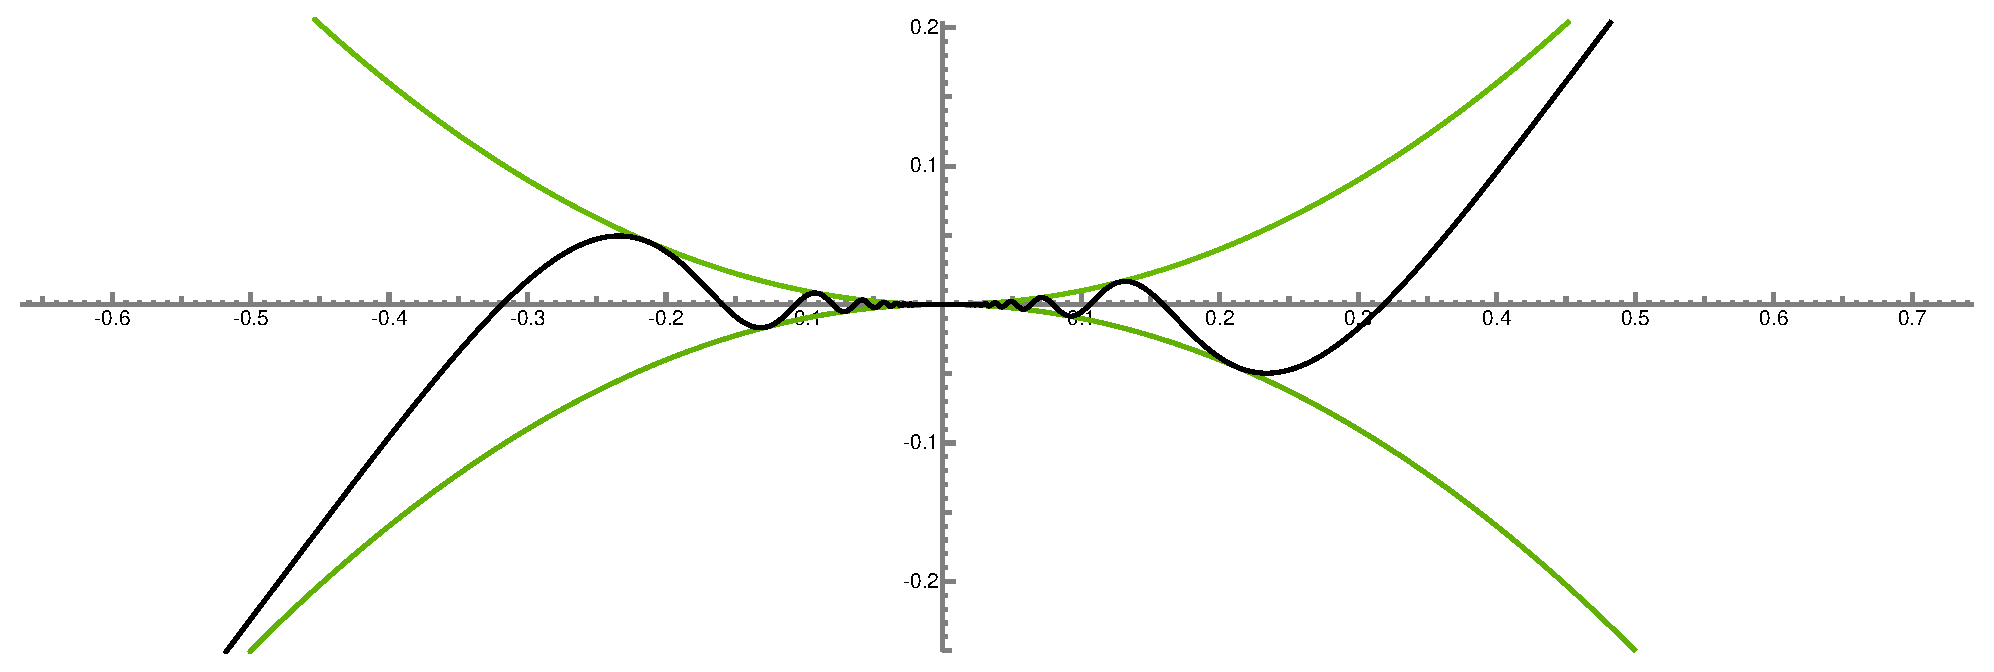
\includegraphics[height=4cm]{darboux.pdf}
  \centering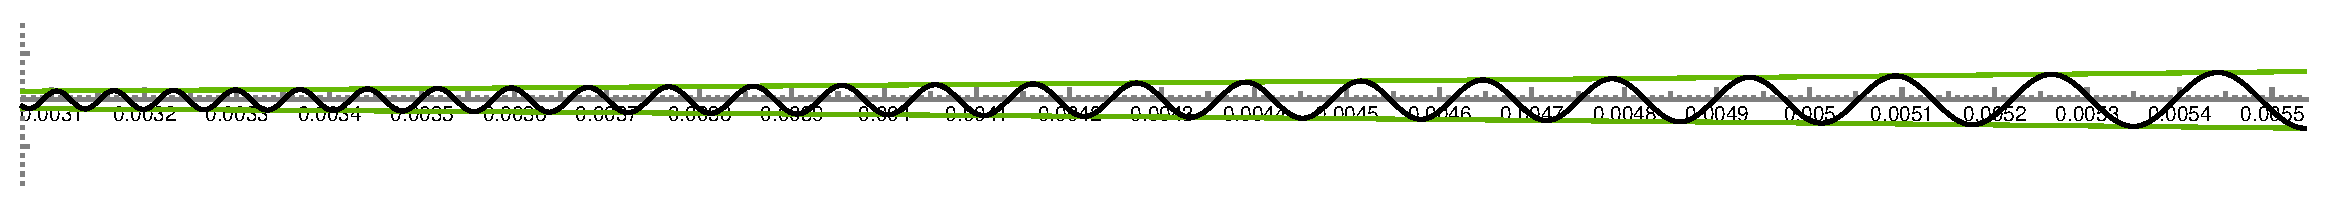
\includegraphics[width=\textwidth]{darboux2.pdf}
  \begin{comment}
  \begin{tikzpicture}[scale=5]
    \draw[->] (-0.5, 0) -- (0.5, 0) node[above] {$x$};
    \draw[->] (0, -0.3) -- (0, 0.3) node[right] {$y$};
    \draw[domain=-0.51:0.5, smooth, variable=\x, gray] plot ({\x}, {\x*\x});
    \draw[domain=-0.51:0.5, smooth, variable=\x, gray] plot ({\x}, {-\x*\x});
    \draw[domain=-0.51:0.5, variable=\x, samples=200, blue, thick] plot ({\x}, {\x*\x*sin(deg(1/\x))});
  \end{tikzpicture}
  \begin{tikzpicture}[scale=5000]
    \draw[->] (0.0045, 0) -- (0.0055, 0) node[above] {$x$};
    \draw[domain=0.0045:0.0055, smooth, variable=\x, gray] plot ({\x}, {\x*\x});
    \draw[domain=0.0045:0.0055, smooth, variable=\x, gray] plot ({\x}, {-\x*\x});
    \draw[domain=0.0045:0.0055, variable=\x, samples=200, blue, thick] plot ({\x}, {\x*\x*sin(deg(1/\x))});
  \end{tikzpicture}
  \end{comment}
  \caption{Il grafico di una funzione derivabile ma con 
    derivata non continua (vedi esempio~\ref{ex:derivata_non_continua}).
    L'ingrandimento nel disegno in basso rende evidente 
    il fatto che la derivata oscilla tra i valori 
    $-1$ e $1$ in ogni intorno di $0$.
    La proprietà di Darboux (teorema~\ref{th:darboux})
    rimane comunque soddisfatta: la derivata assume tutti i valori 
    compresi tra $1$ e $-1$ in ogni intorno di $x=0$ ma 
    non ha limite per $x\to 0$.\\\\
    \usebox{\qrdarboux}
}
\end{figure}

\begin{example}
[funzione derivabile con derivata non continua]
\label{ex:derivata_non_continua}%
\mymark{**}%
\index{funzione!derivabile con derivata non continua}%
\index{derivata!non continua}%
La funzione $f\colon \RR \to \RR$ definita da
\[
  f(x)
  = \begin{cases}
    x^2 \sin(1/x) & \text{se $x \neq 0$} \\
    0 & \text{se $x=0$.}
  \end{cases}
\]
è derivabile su tutto $\RR$, $f'(0)=0$ ma il limite
\[
\lim_{x\to 0} f'(x)
\]
non esiste (e dunque $f'\colon \RR\to\RR$ non è continua in $x=0$).
\end{example}
%
\begin{proof}
La funzione $x^2 \sin(1/x)$ è derivabile infinite volte su tutto il suo dominio $\RR\setminus\ENCLOSE{0}$ in quanto composizione di funzioni elementari derivabili infinite volte.
Dunque, per la località della derivata, anche la funzione $f$ è derivabile infinite volte su $\RR\setminus\ENCLOSE{0}$.
Per $x\neq 0$ possiamo quindi calcolare $f'(x)$ utilizzando le regole di derivazione
\[
  f'(x)
  = D \enclose{x^2\sin \frac 1 x}
  = 2x \sin \frac 1 x + x^2 \enclose{\cos \frac 1 x} \cdot\frac{-1}{x^2}
  = 2x \sin \frac 1 x - \cos \frac 1 x.
\]

Verifichiamo ora che $f$ è continua e derivabile anche in $0$.
Si ha infatti
\[
 \lim_{h\to 0}\frac{f(0+h)-f(0)}{h}
 = \lim_{h\to 0} h \sin \frac 1 h = 0
\]
e dunque $f'(0) = 0$.
Osserviamo però che $f'(x)$ non ammette limite per $x\to 0$
in quanto per $x \to 0$ si ha $2x \sin(1/x) \to 0$ ma il limite di $\cos (1/x)$ invece non esiste. Dunque $f'(x)$ è la somma di una funzione che ha limite zero e di una funzione il cui limite non esiste per $x\to 0$. Dunque $f'(x)$ non ammette limite per $x\to 0$.
\end{proof}

\begin{proposition}[criterio di derivabilità]%
\label{prop:4384774}\mymark{**}%
Sia $I\subset \RR$ un intervallo, $x_0\in I$,
$f\colon I \to \RR$ una funzione continua su tutto $I$ 
e derivabile in $I\setminus\ENCLOSE{x_0}$.
Se il limite della derivata
\[
  \lim_{x\to x_0} f'(x) = m
\]
esiste ed è finito la funzione $f$ è derivabile anche in $x_0$ e vale $f'(x_0) = m$.
\end{proposition}
%
\begin{proof}
\mymark{*}
Prendiamo un generico punto $x>x_0$ (il caso $x<x_0$ è del tutto analogo).
Per il teorema
di Lagrange sappiamo esistere un punto $y\in (x_0,x)$ tale che
\[
  \frac{f(x)-f(x_0)}{x-x_0} = f'(y).
\]
Per $x\to x_0$ si ha certamente anche $y\to x_0$ e dunque
esiste il limite del rapporto incrementale:
\[
  f'(x_0) = \lim_{x\to x_0} \frac{f(x)-f(x_0)}{x-x_0}
  = \lim_{y\to x_0} f'(y) = m.
\]
\end{proof}
%
La proposizione precedente dice che la derivata di una funzione in un
punto non può avere un valore diverso dal suo limite, se tale limite esiste.
Esistono però funzioni derivabili la cui derivata non è
continua, come abbiamo visto
nell'esempio~\ref{ex:derivata_non_continua}
in quanto il limite della derivata potrebbe non esistere.


\section{convessità}
\index{concavo}%
\index{convesso}%

\begin{definition}[funzione convessa]
\mymark{**}
Sia $I\subset \RR$ un intervallo.
Una funzione $f\colon I\to \RR$
si dice essere
\emph{convessa}
\mymargin{funzione convessa}%
\index{funzione!convessa}%
\index{convessa!funzione}%
se per ogni $x,y\in I$ e per ogni $t\in [0,1]$ si ha
\[
f((1-t)x + ty) \le (1-t) f(x) + t f(y).
\]

Analogamente diremo che $f$ è \emph{concava} 
\mymargin{funzione concava}%
\index{funzione!concava}%
\index{concava!funzione}%
se vale la disuguaglianza inversa:
\[
f((1-t)x + ty) \ge (1-t) f(x) + t f(y)
\]
(o, equivalentemente, se $-f$ è convessa).
\end{definition}

Osserviamo che la retta del piano passante per i punti $(x,f(x))$ e $(y,f(y))$ può essere parametrizzata in maniera uniforme per $t\in \RR$
da
\[
  (1-t) (x,f(x)) + t(y,f(y)) = ((1-t)x + ty, (1-t) f(x) + tf(y)).
\]
Chiaramente per $t=0$ si ottiene il punto $(x,f(x))$ per $t=1$ il punto $(y,f(y))$ e per $t\in[0,1]$ il segmento congiungente tali punti. La condizione di convessità della funzione $f$ corrisponde quindi a richiedere che ogni corda (segmento) che unisce due punti del grafico si trovi "al di sopra" del grafico della funzione.

\begin{definition}[insieme convesso]
\mymark{*}
Un insieme $E\subset \RR^n$ si dice essere \emph{convesso}%
\mymargin{convesso}%
\index{convesso} se dati
due punti qualunque $a,b\in E$ l'intero segmento $[a,b]=\ENCLOSE{(1-t)a+tb\colon t\in [0,1]}$ è contenuto in $E$.
\end{definition}

\begin{theorem}[epigrafico delle funzioni convesse]
Sia $I\subset \RR$ e $f\colon I\subset \RR\to \RR$ una funzione.
Allora sono equivalenti:
\begin{enumerate}
\item $I$ è un intervallo e $f$ è convessa;
\item l'\emph{epigrafico di $f$}%
\mymargin{epigrafico di $f$}%
\index{epigrafico}%
(o \emph{sopragrafico})
\index{epigrafico}%
ovvero l'insieme
\[
  E = \ENCLOSE{(x,y)\in \RR^2\colon x\in I, y\ge f(x)}
\]
è convesso.
\end{enumerate}

Per le funzioni concave sarà il \emph{sottografico} $\ENCLOSE{(x,y)\colon y\le f(x)}$ ad essere convesso.
\end{theorem}
%
\begin{proof}
Supponiamo che $I$ sia un intervallo e $f$ sia convessa. 
Per dimostrare che l'epigrafico $E$ è convesso consideriamo due punti $a,b\in E$ 
e un qualunque punto $p$ sul segmento $[a,b]$.
Se $a=(x_a, y_a)$, $b=(x_b,y_b)$, $p=(x_p, y_p)$
allora esiste un $t\in [0,1]$ tale che $x_p = (1-t)x_a + t x_b$ e $y_p=(1-t)y_a + t y_b$.
Visto che $a,b\in E$ sappiamo che $y_a \ge f(x_a)$ e $y_b\ge f(x_b)$. 
Dunque necessariamente si ha
\[
  y_p \ge (1-t)f(x_a) + t f(x_b).
\]
Ma essendo $f$ convessa si ha:
\[
  (1-t)f(x_a) + t f(x_b) \ge f((1-t)x_a + t x_b) = f(x_p).
\]
Dunque $y_p\ge f(x_p)$ che significa $p\in E$.

Viceversa supponiamo di sapere che $E$ è convesso. Siano $x,y\in I$ punti qualunque. Allora i punti $a=(x,f(x))$ e $b=(y,f(y))$ sono certamente punti di $E$ e quindi l'intero segmento $[a,b]$ deve essere contenuto in $E$. Dunque per ogni $t\in [0,1]$ il punto $p = ((1-t)x + t y,$ $(1-t)f(x)+ tf(y))$ deve stare in $E$. In primo luogo deve quindi essere $(1-t)x+ty\in I$ e se questo è vero per ogni $t\in[0,1]$ significa che $I$ è un intervallo. In secondo luogo se $p\in E$ significa che
\[
  (1-t)f(x) +t f(y) \ge f((1-t)x + t y)
\]
che corrisponde alla definizione di funzione convessa.
\end{proof}


\begin{lemma}[rapporto incrementale di una funzione convessa]
\mymark{*}%
\label{lemma:547091}%
Sia $I$ un intervallo di $\RR$ e sia $f\colon I\to \RR$.
Dati $x,y\in I$ con $x\neq y$ definiamo il \emph{rapporto incrementale}
di $f$ come:
\[
  R(x,y) = \frac{f(y) - f(x)}{y-x}.
\]
Allora sono condizioni equivalenti:
\begin{enumerate}
\item $f$ è convessa;
\item per ogni $x,y,z\in I$ se $x<y<z$ si ha $R(x,y)\le R(y,z)$;
\item per ogni $x,y,z\in I$ se $x<y<z$ si ha $R(x,y)\le R(x,z)$;
\item per ogni $x,y,z\in I$ se $x<y<z$ si ha $R(x,z)\le R(y,z)$;
\item la funzione $R(x,y)$ è crescente in ognuna delle due variabili.
\end{enumerate}
\end{lemma}
%
\begin{proof}
Attenzione:
il lemma risulta ovvio se si utilizza la giusta interpretazione geometrica
(il rapporto incrementale è la pendenza della corda corrispondente).
Quella che segue è la traduzione algebrica di quanto
è geometricamente ovvio ma risulta inevitabilmente pesante
e più difficilmente comprensibile.

Siano $x,y,z\in I$ con $x<y<z$.
Posto $t=(y-x)/(z-x)$ si ha $y=(1-t)x + tz$,
 $y-x = t(z-x)$, $z-y = (1-t)(z-x)$.
Si ha allora
 \begin{equation*}
 \begin{aligned}
 R(x,z) - R(x,y)
 &= \frac{f(z)-f(x)}{z-x} - \frac{f(y)-f(x)}{y-x} \\
  &= t\frac{f(z)-f(x)}{y-x} - \frac{f(y)-f(x)}{y-x} \\
  &= \frac{tf(z) + (1-t) f(x) - f(y)}{y-x}
 \end{aligned}
 \end{equation*}

La condizione di convessità di $f$ è
\[
  f(y) \le (1-t)f(x) + tf(z)
\]
ed è quindi equivalente alla condizione $R(x,y) \le R(x,z)$.
Dunque le condizioni 1 e 3 sono equivalenti.

Ma con una verifica diretta si osserva che
\[
  R(x,z) = t R(x,y) + (1-t) R(y,z)
\]
da cui si ottiene
\[
  R(y,z) - R(x,z) = t[R(y,z) - R(x,y)]
\]
oppure anche
\[
 R(x,z) - R(x,y) = (1-t) [R(y,z) - R(x,y)].
\]
Risulta quindi che le quantità
\[
  R(y,z) - R(x,y), \qquad
  R(x,z) - R(x,y), \qquad
  R(y,z) - R(x,z)
\]
hanno tutte lo stesso segno. E quindi le condizioni 2, 3 e 4 sono tra loro equivalenti (se vale una delle tre valgono tutte e tre).

Se valgono le tre condizioni 2, 3 e 4 è facile verificare che la funzione $R(x,y)$ è crescente in entrambe le variabili. Innanzitutto per simmetria, visto che $R(x,y) = R(y,x)$, è sufficiente verificare che $R(x,y)$ è crescente nella seconda variabile $y$ per ogni $x$ fissato. Quindi dato $z>y$ bisogna mostrare che $R(x,z) \ge R(x,y)$.
Abbiamo allora tre possibilità a seconda che sia $x<y$ oppure $y<x<z$ oppure $z<x$. Nel primo caso si ha $x<y<z$ e dunque la disuguaglianza $R(x,y) \le R(x,z)$ corrisponde alla condizione 3.
Nel secondo caso si ha $y<x<z$ e la condizione $R(x,y)\le R(x,z)$ si può scrivere come $R(y,x) \le R(x,z)$ che è, riordinando opportunamente le variabili, la condizione 2. Se, infine, $y < z < x$ la condizione $R(x,y) \le R(x,z)$ si può scrivere $R(y,x) \le R(z,x)$ che, riordinando le variabili, è la condizione 4.

Viceversa (e infine) se la funzione $R(x,y)$ è crescente in entrambe le variabili in particolare è crescente nella seconda variabile e quindi se $x<y<z$ si ha $R(x,y) \le R(x,z)$. Risulta quindi che la condizione 5 implica la 3 e quindi tutte le altre condizioni.
\end{proof}

\begin{theorem}
\mymark{***}
Sia $I\subset \RR$ un intervallo e $f\colon I \to \RR$ una funzione derivabile su tutto $I$.
Allora sono equivalenti:
\begin{enumerate}
\item $f$ è convessa;
\item per ogni $x_0 \in I$ e per ogni $x\in I$ si ha
\[
   f(x) \ge f'(x_0) (x-x_0) + f(x_0)
\]
(geometricamente: il grafico della funzione sta sopra la retta tangente);
\item $f'$ è crescente.
\end{enumerate}

Analogamente per le funzioni concave si avrà che il grafico ``sta sotto'' la retta tangente e che la derivata è decrescente.
\end{theorem}
%
\begin{proof}
\mymark{**}
Osserviamo che
\[
  f'(x_0) = \lim_{x\to x_0} R(x_0,x).
\]
Se $f$ è convessa allora, per il lemma, il rapporto incrementale $R(x_0,x)$ è crescente e quindi  $f'(x_0) = \inf_{x>x_0} R(x_0,x)$. In particolare $f'(x_0) \le R(x_0,x)$ per ogni $x> x_0$. In maniera analoga si trova $f'(x_0) \ge R(x_0,x)$ se $x<x_0$.
In ogni caso risulta quindi che per ogni $x$ si ha
\[
(R(x_0,x)- f'(x_0))(x-x_0)\ge 0
\]
ovvero
\[
  f(x) - f(x_0) - f'(x_0)(x-x_0) \ge 0.
\]
Dunque la condizione 1 implica la 2.

Se vale la condizione 2, dati $x,y \in I$ si ha
\[
  f(x) - f(y) \ge f'(y)(x-y)
\]
se scambiamo $x$ e $y$ e cambiamo di segno ambo i membri si ottiene invece
\[
  f(x) - f(y) \le f'(x)(x-y)
\]
mettendo insieme le due disuguaglianze,
se ora supponiamo che sia $x>y$ otteniamo proprio
$f'(x) \ge f'(y)$ cioè $f'$ è crescente (condizione 3).

Supponiamo ora di sapere che $f'$ è crescente 
e dimostriamo che se $x<y<z$ allora $R(x,y) \le R(y,z)$.
Per il teorema di Lagrange esistono $s\in (x,y)$ 
e $t\in (y,z)$ tali che $f'(s) = R(x,y)$ e $f'(t) = R(y,z)$.
Ma $s<t$ dunque $f'(s) \le f'(t)$ ovvero $R(x,y) \le R(y,z)$
come volevamo dimostrare.
\end{proof}

\begin{corollary}[criterio di convessità tramite derivata seconda]
\mymark{***}
Sia $I\subset \RR$ un intervallo e sia $f\colon I \to \RR$ una funzione derivabile due volte (cioè $f$ è derivabile e anche $f'$ è derivabile).
Allora $f$ è convessa se e solo se $f''(x)\ge 0$ per ogni $x\in I$.
Analogamente $f$ è concava se e solo se $f''\le 0$.
\end{corollary}
\begin{proof}
\mymark{***}
Per il criterio precedente $f$ è convessa se e solo se $f'$ è crescente. Per il criterio di monotonia $f'$ è crescente se e solo se $f'' \ge 0$. Considerazioni analoghe valgono per la concavità.
\end{proof}

\begin{theorem}
Siano $a\in \RR$, $b\in \bar \RR$, $a<b$.
Sia $f\colon [a,b)\to \RR$ una funzione convessa 
in $(a,b)$ e continua in $a$. 
Allora $f$ è convessa su tutto $[a,b)$. 
Risultato analogo vale per funzioni definite su 
intervalli aperti a sinistra $(a,b]$
o su intervalli aperti da ambo i lati $(a,b)$.
\end{theorem}
%
\begin{proof}
Basta dimostrare che se $x<y<z$ allora $R(x,y)\le R(y,z)$.
La disuguaglianza è valida per $x>a$ essendo $f$ convessa 
in $(a,b)$ e dunque, passando al limite per $x\to a$, 
grazie alla continuità di $f$ in $a$,
la disuguaglianza risulta dimostrata anche quando $x=a$.
\end{proof}

\begin{example}
La funzione $f(x) = \sqrt{x}$ è definita su $[0,+\infty)$ ma è derivabile solamente in $(0,+\infty)$. La sua derivata è $f'(x) = x^{-\frac 1 2 }/2$ e la derivata seconda è $f''(x) = -x^{-\frac 3 2}/4 < 0$. Dunque la funzione è concava sull'intervallo aperto $(0,+\infty)$. Ma essendo continua possiamo concludere che $f$ è concava su tutto il dominio $[0,+\infty)$.
\end{example}

\begin{comment}
\begin{theorem}[continuità delle funzioni convesse]
Siano $a,b \in \bar \RR$ con $a< b$.
Sia $f\colon (a,b) \to \RR$ una funzione convessa. Allora $f$ è continua.
\end{theorem}
%
\begin{proof}
Sia $x_0 \in (a,b)$ e siano $y,z \in (a,b)$ con $y < x_0 < z$.
Per il lemma sui rapporti incrementali sappiamo che per ogni $x\in (y,z)$ si ha
\[
   R(x_0, y) \le R(x_0,x) \le R(x_0,z).
\]
In particolare esiste una costante $C$ tale che
\[
  \abs{R(x_0,x)} \le C,\qquad \forall x \in (y,z).
\]
Moltiplicando per $\abs{x-x_0}$ si ottiene allora
\[
   \abs{f(x) - f(x_0)} \le C \abs{x-x_0}
\]
e per $x\to x_0$ il lato destro tende a zero e quindi per confronto anche il lato sinistro deve tendere a zero. Dunque $f(x)\to f(x_0)$
e $f$ è continua in $x_0$.
\end{proof}
\end{comment}

\begin{theorem}[derivabilità delle funzioni convesse]
  Sia $I\subset \RR$ un intervallo e sia $f\colon I \to \RR$ una funzione convessa.
  Se $x_0\in (\inf I, \sup I)$ esistono e sono finite la derivata destra 
  e sinistra di $f$ in $x_0$:
  \begin{align*}
    f'_+(x_0) &= \lim_{x\to x_0^+} \frac{f(x)-f(x_0)}{x-x_0}\\
    f'_-(x_0)  &= \lim_{x\to x_0^-} \frac{f(x)-f(x_0)}{x-x_0}  
  \end{align*}
  e risulta
  \[
    f'_-(x_0) \le f'_+(x_0).
  \]
  Inoltre se $\inf I < x_1 < x_2 < \sup I$ si ha 
  \[
    f'_+(x_1) \le f'_-(x_2).
  \]
  Se ne deduce che $f$ è continua in tutti i punti interni di $I$ 
  e che l'insieme dei punti in cui $f$ non è derivabile 
  è al più numerabile.
  \end{theorem}
  %
  \begin{proof}
    Nel lemma~\ref{lemma:547091} abbiamo osservato che il rapporto incrementale
    \[
      R(x_0,x) = \frac{f(x)-f(x_0)}{x-x_0}
    \] 
    di una funzione convessa è crescente rispetto alla variabile $x$. 
    Dunque per il teorema~\ref{th:limite_monotona} si 
    ha 
    \[
      f'_-(x_0) = \sup_{x<x_0} R(x_0,x)>-\infty, \qquad 
      f'_+(x_0) = \inf_{x>x_0} R(x_0,x)<+\infty
    \]
    e visto che se $x<x_0$ e $y>x_0$ si ha $R(x_0,x)\le R(x_0,y)$ 
    deduciamo che $f'_-(x_0)\le f'_+(x_0)$ ed entrambi i limiti 
    sono dunque finiti. Se $x_1 < x_2$ allora preso un qualunque 
    punto $x$ con $x_1<x<x_2$ si ha (sempre per il lemma~\ref{lemma:547091})
    \[
      R(x_1,x) \le R(x,x_2)
    \]
    e dunque passando al limite si trova $f'_+(x_1) \le f'_-(x_2)$.
    Le derivate destra e sinistra esistono dunque in tutti i punti interni 
    all'intervallo $I$. 
    In particolare $f$ è continua in tali punti in quanto è continua sia da destra 
    che da sinistra.
    I punti di non derivabilità di $f$ sono i punti in cui 
    le derivate destra e sinistra differiscono. 
    Ma ad ogni punto $x$ di non differenziabilità 
    posso associare l'intervallo aperto non vuoto $I_x = (f'_-(x),f'_+(x))$ e per 
    le proprietà appena viste è chiaro che questi intervalli sono a due a due disgiunti
    in quanto se $x_1<x_2$ l'estremo destro di $I_{x_1}$ è minore o uguale all'estremo 
    sinistro di $I_{x_2}$.
    Siccome ognuno di questi intervalli contiene almeno un numero razionale concludiamo che 
    il numero di punti di discontinuità non può essere maggiore della cardinalità 
    dei numeri razionali.
  \end{proof}
  
  \begin{theorem}[retta di supporto]
    \label{th:supporto_convessa}%
    Sia $I\subset \RR$ un intervallo, $f\colon I\to\RR$ una funzione convessa 
    e $x_0$ un punto interno ad $I$. Allora esiste una funzione lineare affine 
    \[
      L(x) = mx+q
    \]
    tale che $f(x_0) = L(x_0)$ e per ogni $x\in I$ si abbia $f(x)\ge L(x)$.
  \end{theorem}
  %
  \begin{proof}
    Basta scegliere qualunque $m\in [f'_-(x_0),f'_+(x_0)]$ e considerare la funzione 
    lineare affine $L(x) = m(x-x_0) + f(x_0)$. Se $x>x_0$ allora si ha $R(x_0,x)\ge m$ 
    e dunque $f(x) - f(x_0) \ge m (x-x_0) = L(x)$. Viceversa se $x<x_0$ 
    si ha $R(x_0,x)\le m$ da cui, di nuovo, $f(x)-f(x_0) \ge m(x-x_0) = L(x)$.
  \end{proof}
  %
  Il seguente teorema può essere enunciato anche per gli integrali 
  come vedremo nel teorema~\ref{th:jensen}. 
  La dimostrazione è sostanzialmente identica ed è valida anche 
  per funzioni convesse di più variabili.
  %
  \begin{theorem}[combinazioni baricentriche/disuguaglianza di Jensen]
    \mymark{*}%
    \label{th:combinazioni_baricentriche}%
    \index{combinazioni baricentriche}%
    \index{disuguaglianza!di Jensen}%
    \index{Jensen!disuguaglianza di}%
    Se $f$ è una funzione convessa definita su un intervallo $I$, dati $x_1, \dots, x_n \in I$ e $\lambda_1, \dots, \lambda_n\in \RR$ tali che $\sum_{k=1}^n \lambda_k = 1$ e $\lambda_k \ge 0$ per ogni $k=1, \dots, n$ allora
    \[
      f\enclose{\sum_{k=1}^n \lambda_k x_k}
      \le \sum_{k=1}^n \lambda_k f(x_k).
    \]
    Per le funzioni concave vale la disuguaglianza inversa.
    \end{theorem}
    %
    \begin{comment}
    \begin{proof}
    Procediamo per induzione su $n$. Nel caso $n=1$ si ha $\lambda_1=1$ e i due lati della disuguaglianza sono effettivamente uguali. Supponendo il teorema dimostrato per un certo $n$, procediamo a dimostrarlo per $n+1$.
    Osserviamo che
    \begin{align*}
      \sum_{k=1}^{n+1} \lambda_k x_k
      &= \sum_{k=1}^n \lambda_k x_k  + \lambda_{n+1} x_{n+1} \\
      &= (1-\lambda_{n+1})\sum_{k=1}^n\frac{\lambda_k}{1-\lambda_{n+1}} x_k + \lambda_{n+1} x_{n+1}.
    \end{align*}
    Visto che
    \[
      \sum_{k=1}^{n+1} \lambda_k = 1
    \]
    si ha
    \[
      \sum_{k=1}^n \frac{\lambda_k}{1-\lambda_{n+1}}
      = \frac{1-\lambda_{n+1}}{1-\lambda_{n+1}} = 1.
    \]
    Dunque, per ipotesi induttiva si ha allora
    \[
      f\enclose{\sum_{k=1}^n\frac{\lambda_k}{1-\lambda_{n+1}} x_k}
      \le \sum_{k=1}^n \frac{\lambda_k}{1-\lambda_{n+1}}f(x_k).
    \]
    Usando di nuovo la convessità di $f$ con $t=\lambda_{n+1}$ si ha
    \begin{align*}
    f\enclose{\sum_{k=1}^{n+1} \lambda_k x_k}
    &=f\enclose{(1-\lambda_{n+1})\sum_{k=1}^n \frac{\lambda_k}{1-\lambda_{n+1}}x_k + \lambda_{n+1}x_{n+1}}\\
    &\le (1-\lambda_{n+1})f\enclose{\sum_{k=1}^n \frac{\lambda_k}{1-\lambda_{n+1}}x_k} + \lambda_{n+1}f(x_{n+1}) \\
    &\le (1-\lambda_{n+1})\sum_{k=1}^n \frac{\lambda_k}{1-\lambda_{n+1}} f(x_k) + \lambda_{n+1} f(x_{n+1})\\
    &= \sum_{k=1}^{n+1}\lambda_k f(x_k).
    \end{align*}
    come volevamo dimostrare.
    \end{proof}
  \end{comment}
  %    
  \begin{proof}
  Poniamo 
  \[
    \bar x =  \sum_{k=1}^n \lambda_k x_k.
  \]
  Per il teorema~\ref{th:supporto_convessa} precedente 
  sappiamo che esiste una retta $L(x) = mx + q$ 
  tale che $L(\bar x) = f(\bar x)$ 
  e $L(x)\le f(x)$ per ogni $x \in I$.
  Allora si ha 
  \[
  L \enclose{\sum_{k=1}^n \lambda_k x_k}
  = \sum_{k=1}^n m \lambda_k x_k + q \sum_{k=1}^n \lambda_k 
  = \sum_{k=1}^n \lambda_k L(x_k).  
  \]
  Dunque 
  \[
  f(\bar x) = L(\bar x) = \sum_{k=1}^n \lambda_k L(x_k) \le 
  \sum_{k=1}^n \lambda_k f(x_k).
  \]
  \end{proof}

\begin{example}[disuguaglianza tra media aritmetica e media geometrica]
\label{ex:AMGM}%
  \mymark{*}%
\index{disuguaglianza!media aritmetica media geometrica}%
Osserviamo che la funzione $f(x) = \ln x$ è concava, infatti si ha
$f''(x) = -1/x^2 < 0$. Dunque, per il teorema precedente, se $\lambda_1 + \dots + \lambda_n =1$, $\lambda_k \ge 0$ si ha
\[
    \ln\enclose{\sum_{k=1}^n \lambda_k x_k}
    \ge \sum_{k=1}^n \lambda_k \ln x_k.
\]
Facendo l'esponenziale di ambo i membri si ottiene
\[
  \sum_{k=1}^n \lambda_k x_k \ge \prod_{k=1}^n x_k^{\lambda_k}.
\]
Nel caso particolare $\lambda_k = 1/n$ si ottiene
la disuguaglianza tra \emph{media aritmetica} (AM per gli anglofoni)
e \emph{media geometrica}
\mymargin{media aritmetica geometrica}%
\index{media aritmetica geometrica}%
\index{media!aritmetica}%
\index{media!geometrica}%
\index{AM}%
\index{GM}%
(GM):
\[
  \frac{x_1 + \dots + x_n}{n} \ge \sqrt[n]{x_1\cdots x_n}.
\]
\end{example}

\begin{exercise}[subadditività delle funzioni concave]
\index{subadditività!delle funzioni concave}%
\index{funzione!concava!subadditiva}%
\index{concavo!subadditiva}%
Sia $f\colon [0,+\infty) \to \RR$ una funzione concava con $f(0)\ge 0$. Allora $f$ è subadditiva cioè:
\[
  f(x+y) \le f(x) + f(y),\qquad \forall x,y\ge 0.
\]
\end{exercise}
%
\begin{proof}
Se $x=y=0$ la disuguaglianza è ovvia.
Altrimenti $x+y>0$ e si ha
\begin{align*}
f(x) &= f\enclose{\frac{y}{x+y}\cdot 0 + \frac{x}{x+y}\cdot (x+y)}\\ &\ge \frac{y}{x+y}f(0) + \frac{x}{x+y}f(x+y)
\ge \frac{x}{x+y}f(x+y).
\end{align*}
Scambiando $x$ con $y$ e sommando si ottiene:
\[
  f(x) + f(y) \ge \frac{x}{x+y}f(x+y) + \frac{y}{x+y}f(x+y) = f(x+y).
\]
\end{proof}

Si osservi che sviluppando la disuguaglianza $(x-y)^2\ge 0$ si ottiene:
\[
  x y \le \frac{x^2 + y^2}{2}.
\]
Questa disuguaglianza può essere generalizzata ad esponenti diversi 
come si vede nel seguente.

\begin{theorem}[disuguaglianza di Young]%
\label{th:young}%
\index{Young!disuguaglianza di}%
\index{disuguaglianza!di Young}%
Se $p>1$, $q>1$, $\frac{1}{p}+\frac{1}{q}=1$, $x,y\ge 0$:
\begin{equation}\label{eq:young}
  x y \le \frac{x^p}{p} + \frac{y^q}{q}.
\end{equation}
\end{theorem}
%
\begin{proof}
Si utilizza la disuguaglianza di convessità per la funzione $\exp(x)=e^x$. 
Visto che la derivata seconda dell'esponenziale è positiva, la funzione $\exp$ 
è convessa e dunque, se $x>0$ e $y>0$ si ha:
\begin{align*}
 x\cdot y 
  &= \exp(\ln x + \ln y)
  = \exp\enclose{\frac 1 p \ln (x^p) + \frac 1 q \ln (y^q)}  \\
  &\le \frac 1 p \cdot \exp \ln (x^p) + \frac 1 q \exp \ln (y^q)
  = \frac{x^p}{p} + \frac{y^q}{q}.
\end{align*}
Se $x=0$ o $y=0$ la disuguaglianza è ovvia in quanto il lato sinistro 
di~\eqref{eq:young} è nullo.
\end{proof}

\begin{theorem}[disuguaglianza di Hölder]
Se $a_k\ge 0$ e $b_k\ge 0$ per $k\in \NN$
e siano $p>1$ e $q>1$ tali che $\frac 1 p + \frac 1 q = 1$.
Allora 
\[
 \sum_k a_k b_k  \le \enclose{\sum_k a_k^p}^{1 \over p} \cdot \enclose{\sum_k b_k^q}^{1\over q}.
\]
\end{theorem}
\begin{proof}
Poniamo 
\[
A = \enclose{\sum_k a_k^p}^{1 \over p}, \qquad 
B = \enclose{\sum_k b_k^q}^{1\over q}.
\]
Se $A>0$ e $B>0$ possiamo dividere il lato sinistro della disuguaglianza 
per il lato destro e applicare la disuguaglianza~\eqref{eq:young} di Young:
\begin{align*}
  \frac{\sum_k a_k b_k}{A\cdot B} 
  & = \sum_k \frac{a_k}{A}\cdot \frac{b_k}{B} 
  \le \sum_k \frac 1 p \frac{a_k^p}{A^p} + \frac 1 q \frac{b_k^q}{B^q} \\
  &= \frac 1 p \frac{\sum_k a_k^p}{A^p} + \frac 1 q \frac{\sum_k b_k^q}{B^q}
  = \frac 1 p + \frac 1 q = 1.
\end{align*}
E il teorema e dimostrato. 

Se fosse $A=0$ tutti i termini $a_k$ sarebbero nulli e la disuguaglianza 
si riduce banalmente a $0\le 0$. Lo stesso se fosse $B=0$.  
\end{proof}

Nel caso $p=q=2$ si ottiene la 
\emph{disuguaglianza di Cauchy-Schwarz}%
\mymargin{disuguaglianza di Cauchy-Schwarz}%
\index{disuguaglianza!di Cauchy-Schwarz}
\index{disuguaglianza!di Cauchy-Schwarz}%
\index{Cauchy-Schwarz!disuguaglianza di}%
\index{Schwarz!disuguaglianza di Cauchy-}%
\[
   \sum_k \abs{a_k b_k} \le \sqrt{\sum_k a_k^2} \cdot \sqrt{\sum_k b_k^2}
\]
che potrebbe però essere più facilmente dimostrata 
per un generico prodotto scalare, come faremo 
nel teorema~\ref{th:spazio_euclideo}.


\section{teoremi di Cauchy e de l'Hospital}

\begin{theorem}[Cauchy]
\label{th:cauchy}%
\mymark{**}%
\index{teorema!di Cauchy}%
\mymargin{Cauchy}%
\index{Cauchy}%
Siano $a,b\in \RR$, $a < b$.
\mynote{Se $b<a$ il teorema è ugualmente valido intendendo $[a,b]=[b,a]$.}%
Siano $f\colon[a,b]\to \RR$ e $g\colon[a,b]\to \RR$ funzioni continue su tutto $[a,b]$ e derivabili su $(a,b)$.
Supponiamo inoltre che $g'(x)\neq 0$ per ogni $x\in (a,b)$.
Allora $g(b) \neq g(a)$ ed esiste $x_0\in(a,b)$ tale che
\[
  \frac{f'(x_0)}{g'(x_0)} = \frac{f(b)-f(a)}{g(b)-g(a)}.
\]
\end{theorem}
%
\begin{proof}
\mymark{**}
Si consideri la funzione ausiliaria
\[
 h(x) = (g(b)-g(a))f(x) - (f(b)-f(a))g(x).
\]
Per verifica diretta si osserva che
\[
  h(b) = g(b)f(a) - f(b)g(a) = h(a).
\]
Dunque $h$ verifica le ipotesi del teorema di Rolle ed esiste
dunque un punto $x_0\in(a,b)$ per cui $h'(x_0) = 0$.
Essendo però
\[
  h'(x) = (g(b) - g(a)) f'(x) - (f(b)-f(a)) g'(x)
\]
si ottiene
\[
 (g(b)-g(a))f'(x_0) = (f(b) - f(a))g'(x_0).
\]
Per ipotesi sappiamo che $g'(x_0)\neq 0$.
Ma necessariamente anche $g(b) - g(a)\neq 0$ perché altrimenti potremmo applicare il teorema di Rolle alla funzione $g$ e ottenere che $g'$ si annulla in un punto di $(a,b)$, cosa che abbiamo escluso per ipotesi.
Dunque possiamo dividere ambo i membri per $(g(b)-g(a))$ e per $g'(x_0)$ per ottenere l'uguaglianza enunciata nel teorema.
\end{proof}

\begin{theorem}[de l'Hospital $0/0$]
\mymark{***}
Sia $I\subset \RR$ un intervallo, $x_0\in [-\infty,+\infty]$ un punto di accumulazione
di $I$
e siano $f,g \colon I\setminus\ENCLOSE{x_0} \to \RR$ funzioni derivabili.
Supponiamo che sia $g'(x)\neq 0$ per ogni $x\in I\setminus\ENCLOSE{x_0}$.
Se
\[
  \lim_{x\to x_0} f(x) = 0 \qquad \text{e}\qquad \lim_{x\to x_0} g(x) = 0
\]
e se esiste (finito o infinito) il limite
\[
  \ell = \lim_{x\to x_0}\frac{f'(x)}{g'(x)}
\]
allora si ha
\[
  \lim_{x\to x_0} \frac{f(x)}{g(x)} = \ell.
\]
\end{theorem}
%
\begin{proof}
\mymark{**}
Bisognerà distinguere diversi casi a seconda che $x_0$ sia finito o infinito
e che sia un punto interno o un estremo dell'intervallo $I$.
Fatta la dimostrazione nel primo caso tutti gli altri si riconducono ad esso.

\emph{Caso 1:} supponiamo che sia $I=[x_0, b]$. In questo caso possiamo
estendere le funzioni $f$ e $g$ anche nel punto $x_0$ ponendo:
\[
\tilde f(x) =
\begin{cases}
  f(x) & \text{se $x\in (x_0,b]$}\\
  0 & \text{se $x=x_0$,}
\end{cases}
\qquad
\tilde g(x) =
\begin{cases}
  g(x) & \text{se $x\in (x_0,b]$}\\
  0 & \text{se $x=x_0$.}
\end{cases}
\]
Visto che per ipotesi $f(x) \to 0$ e $g(x)\to 0$ per $x\to x_0$ risulta
che $\tilde f$ e $\tilde g$ siano funzioni continue su tutto l'intervallo $[x_0,b]$
inoltre, sempre per ipotesi, sono derivabili nell'intervallo $(x_0,b]$
visto che l'estensione per $x=x_0$ non modifica le derivate negli altri punti.
In particolare le funzioni estese soddisfano le ipotesi del teorema di Cauchy in
ogni intervallo $[x_0,x]$ con $x\in (x_0,b]$, dunque possiamo affermare
che per ogni $x$ esiste $c(x)\in (x_0,x)$ tale che
\[
  \frac{f(x)}{g(x)}
  = \frac{\tilde f(x) - \tilde f(x_0)}
  {\tilde g(x)- \tilde g(x_0)}
  = \frac{\tilde f'(c(x))}{\tilde g'(c(x))}
  = \frac{f'(c(x))}{g'(c(x))}.
\]
Ma essendo $x_0< c(x) < x$ per $x\to x_0$ si ha $c(x)\to x_0$ e quindi,
tramite un cambio di variabile
(Teorema~\ref{th:limite_composta})
possiamo affermare che
\[
    \lim_{x\to x_0} \frac{f(x)}{g(x)}
  = \lim_{x\to x_0}\frac{f'(c(x))}{g'(c(x))}
  = \lim_{x\to x_0}\frac{f'(x)}{g'(x)} = \ell.
\]

\emph{Caso 2:} supponiamo sia $I$ qualunque e $x_0$ finito.
Visto che le funzioni sono definite su $I\setminus\ENCLOSE{x_0}$ possiamo sempre
supporre $x_0\in I$. Inoltre
visto che i limiti dipendono solo dai valori in un intorno del punto $x_0$
possiamo sempre supporre che $I$ sia un intervallo chiuso e limitato.
Nel passo precedente abbiamo fatto il caso in cui $x_0$ era l'estremo
inferiore di $I$, ma allo stesso modo si può fare il caso in cui
$x_0$ è l'estremo superiore. Se invece $x_0$ fosse un punto interno di $I$
possiamo considerare separatamente il limite destro e sinistro e ricondurci
ai casi in cui $x_0$ era un estremo.

\emph{Caso 3:} supponiamo sia $x_0=+\infty$. In tal caso
l'intervallo $I$ contiene un intevallo $[a,+\infty)$ con $a\in\RR$.
Anche in questo caso vogliamo ricondurci al primo caso tramite il cambio
di variabile $t=1/x$. Posto $F(t) = f(1/t)$ e $G(t)= g(1/t)$ si osserva che $F$ e $G$
sono definite sull'intervallo $(0,1/a]$,
tendono a zero per $t\to 0^+$
sono derivabili,
\[
  F'(t) = -\frac{f'(1/t)}{t^2}, \qquad
  G'(t) = -\frac{g'(1/t))}{t^2}
\]
e risulta quindi
\[
  \lim_{t\to 0^+} \frac{F'(t)}{G'(t)}
  = \lim_{t\to 0^+} \frac{f'(1/t)}{g'(1/t)}
  = \lim_{x\to +\infty} \frac{f'(x)}{g'(x)} = \ell.
\]
Quindi applicano il teorema nel caso già dimostrato possiamo affermare che
\[
  \lim_{x\to +\infty} \frac{f(x)}{g(x)} = \lim_{t\to 0^+} \frac{F(t)}{G(t)} = \ell.
\]

\emph{Caso 4:} il caso $x_0 = -\infty$ si svolge in maniera analoga al caso precedente.
\end{proof}

\begin{theorem}[de l'Hospital $\cdot/\infty$]
\mymark{*}
\index{teorema!di de l'Hospital}
\mymargin{de l'Hospital}%
\index{de l'Hospital}
Siano $a,b\in [-\infty,+\infty]$ con $a<b$.
Siano $f,g \colon (a,b)\to \RR$ funzioni derivabili.
Se
\[
 \lim_{x\to a^+} \abs{g(x)} = +\infty,
\]
se $g'(x) \neq 0$ per ogni $x\in (a,b)$
e se esiste il limite (finito o infinito)
\[
  \ell = \lim_{x\to a^+}\frac{f'(x)}{g'(x)}
\]
allora
si ha
\[
 \lim_{x\to a^+}\frac{f(x)}{g(x)} = \ell.
\]

Risultato analogo si ha facendo i limiti per $x\to b^-$ invece che per $x\to a^+$ e di conseguenza anche nel caso in cui la funzione sia definita su un intervallo ``bucato''
$f\colon (a,b)\setminus\ENCLOSE{x_0} \to \RR$ e si considerino i limiti ``pieni'' per $x\to x_0$.
\end{theorem}
%
\begin{proof}
Supponiamo per assurdo che non si abbia
\[
  \lim_{x\to a^+} \frac{f(x)}{g(x)} = \ell.
\]
Allora, per il teorema di collegamento tra limiti di funzione e limiti di successione, deve esistere una successione $a_k\in (a,b)$, $a_k\to a$ tale che non si abbia
\[
  \lim_{k\to +\infty} \frac{f(a_k)}{g(a_k)} = \ell.
\]
Se la successione $f(a_k) / g(a_k)$ è limitata allora applicando il teorema di Bolzano Weierstrass sappiamo esistere una sottosuccessione
convergente ad un valore $m\neq \ell$ (se tutte le sottosuccessioni convergessero ad $\ell$ l'intera successione convergerebbe ad $\ell$).
Se invece $f(a_k) / g(a_k)$ non è limitata possiamo estrarre una sottosuccessione che converge a $+\infty$ oppure a $-\infty$. In ogni caso esiste una successione, che chiameremo ancora $a_k$, ed esiste $m\in \bar \RR$ tale che
\[
  \lim_{k \to +\infty} \frac{f(a_k)}{g(a_k)} = m \neq \ell.
\]
Consideriamo ora un intorno $U$ di $m$ e un intorno $V$ di $\ell$ tali che $U\cap V = \emptyset$.
Siccome $f'(x) / g'(x) \to \ell$ per $x\to a$ esiste un $c\in (a,b)$ tale che per ogni $x\in (a,c)$ si ha
\[
  \frac{f'(x)}{g'(x)} \in V.
\]
Consideriamo allora il seguente rapporto incrementale
\begin{align*}
\frac{f(a_k) - f(x)}{g(a_k) - g(x)}
=\frac{\frac{f(a_k)}{g(a_k)}-\frac{f(x)}{g(a_k)}}{1-\frac{g(x)}{g(a_k)}}
\end{align*}
e osserviamo che il lato destro tende a $m$ per $k\to +\infty$ in quanto $f(a_k)/g(a_k) \to m$ e visto che $\abs{g(a_k)}\to +\infty$ si ha $f(x)/g(a_k)\to 0$ e $g(x)/g(a_k) \to 0$.
Dunque esisterà un $k$ per cui il lato destro sta nell'intorno $U$ di $m$. Al lato sinistro possiamo invece applicare il teorema di Cauchy e trovare quindi un punto $y\in(a_k,c)$ per cui tale lato risulti
uguale a $f'(y)/g'(y)$. Ma visto che $y\in (a,c)$ si dovrà avere $f'(y)/g'(y) \in V$. Questo è assurdo in quanto $U\cap V = \emptyset$.
\end{proof}


\section{classi di regolarità}

Sia $A\subset \RR$ e sia $f\colon A\to \RR$ una funzione definita su $A$.
Diremo che $f$ è di classe $C^0$ se $f$ è continua. 
Possiamo definire $C^0(A)$ come l'insieme delle funzioni continue definite 
su $A$ (a valori in $\RR$).
Se $f$ è derivabile (su tutto $A$) e la derivata di $f$ è anch'essa continua 
(su tutto $A$) diremo che 
$f$ è di classe $C^1$ e scriveremo $f\in C^1(A)$.
Andando avanti: se $f$ è derivabile e anche $f'$ è derivabile e se la derivata 
seconda $f''$ è continua, diremo che $f$ è di classe $C^2$. 
E così via.

E' importante osservare che $C^1(A)$ non coincide con l'insieme delle funzioni 
derivabili su $A$. 
Infatti abbiamo già visto nell'esempio~\ref{ex:derivata_non_continua} 
che esistono funzioni derivabili la cui derivata non è continua 
e quindi tali funzioni, pur essendo derivabili, non sono di classe $C^1$.


Per definire formalmente l'insieme delle funzioni di classe $C^k$ 
per ogni $k\in \NN$ dobbiamo dare una definizione per induzione.
Definiamo inoltre la classe $C^{\infty}(A)$ che è l'insieme delle funzioni 
che sono derivabili $k$ volte per ogni $k\in \NN$.
%
\begin{definition}[funzioni di classe $C^k$]
\mymark{**}
Dato $A\subset \RR$ denotiamo con $\RR^A$ l'insieme di tutte le funzioni $f\colon A \to \RR$.
Per ogni $k\in \NN$ definiamo
$C^k(A) \subset \RR^A$ nel modo seguente:
\mymargin{$C^k$}%
\index{$C^k$}
\begin{enumerate}
\item se $k=0$ poniamo
\[
  C^0(A) = \ENCLOSE{f\in \RR^A \colon \text{$f$ continua}}.
\]
\item
  se $k>0$ definiamo induttivamente
  \[
  C^{k}(A) = \ENCLOSE{f\in \RR^A \colon \text{$f$ derivabile e $f'\in C^{k-1}(A)$}}.
  \]
\end{enumerate}
Chiaramente se $j\ge k$ si ha $C^j(A) \subset C^k(A)$ dunque $C^k(A)$ è una famiglia decrescente (rispetto all'inclusione insiemistica) ed ha senso definire:
\mymargin{$C^\infty$}%
\index{$C^\infty$}
\[
  C^\infty(A) = \ENCLOSE{f\in \RR^A\colon \forall k \in \NN\colon f\in C^k(A)} = \bigcap_{k\in \NN} C^k(A).
\]

Le funzioni $f\in C^k(A)$ sono derivabili $k$ volte.
Utilizziamo la notazione $f^{(j)}$%
\mymargin{$f^{(j)}$}%
\index{$f^{(j)}$} per denotare la $j$-esima derivata
di una funzione $f$.
Dunque avremo
\[
  f^{(0)} = f, \qquad
  f^{(1)} = f', \qquad
  f^{(2)} = f'', \dots
\]
\end{definition}

Abbiamo già osservato che $\RR^A$ è uno spazio vettoriale reale.
Gli spazi $C^k(A)$ per $k=0, \dots, \infty$ sono una famiglia decrescente di sottospazi vettoriali di $\RR^A$.
Infatti sappiamo che la combinazione lineare di funzioni continue è continua e che la combinazione lineare di funzioni derivabili è derivabile.

\begin{theorem}
Le funzioni $x$, $e^x$, $\ln x$, $\sin x$, $\cos x$, $\tg x$, $\arctg x$ 
sono di classe $C^\infty$. 
Somma, differenza, prodotto, rapporto, e composizione di funzioni di classe $C^n$ 
sono anch'esse di classe $C^n$ per $n=0,1,2,\dots,\infty$.
\end{theorem}
\begin{proof}
Verifichiamo per induzione che se $f,g \in C^n$ allora $f+g \in C^n$.
Per $n=0$ sappiamo che la somma di funzioni continue è continua: $f,g\in C^0$ implica $f+g\in C^0$.
Per $n>1$ se $f,g\in C^n$ allora $f$ e $g$ sono derivabili e si ha 
$(f+g)'=f'+g'$ (teorema~\ref{th:derivate_operazioni}).
Ma per definizione di $C^n$ si ha $f',g'\in C^{n-1}$ e per ipotesi induttiva 
$f'+g'\in C^{n-1}$ dunque $f+g\in C^n$.

Dimostrazione analoga si può fare per il prodotto $f\cdot g$ osservando 
che $(f\cdot g)' = f'g + fg'$ e che se $f,g\in C^n$ allora $f',g'\in C^{n-1}$ 
dunque $f'g,fg'\in C^{n-1}$ e $f'g+fg'\in C^{n-1}$.

Stessa cosa per la composizione visto che $(f\circ g)' = (f'\circ g)\cdot g'$.

Dunque somma, prodotto e composizione di funzioni di classe $C^n$ sono di classe $C^n$
e lo stesso vale dunque per le funzioni di classe $C^\infty$.

Notiamo ora che le funzioni $-x$ e $\frac 1 x$ sono di classe $C^\infty$
(possiamo esplicitamente calcolarne le derivate di ordine qualunque) e quindi 
se $f\in C^n$ anche $-f$ e $\frac 1 f$ sono di classe $C^n$ per la proprietà della 
composizione. 
Ne segue che anche la differenza e il rapporto di funzioni di classe $C^n$   
è di classe $C^n$.

Possiamo quindi prendere in considerazione le funzioni elementari elencate nell'enunciato 
e osservare che sono tutte funzioni derivabili e che la loro derivata si scrive 
come somma, prodotto, rapporto o composizione delle stesse funzioni elementari.
Dunque se tutte queste funzioni sono di classe $C^n$ allora anche la loro derivata 
è di classe $C^n$. 
Ma se la derivata è di classe $C^n$ allora la funzione è di classe $C^{n+1}$
e dunque, per induzione, tutte le funzioni elementari sono di classe $C^\infty$.
\end{proof}

\begin{example}
  La funzione 
  \[
    \frac{e^{x-\arctg x^2}}{1+\ln x}
  \]
  è di classe $C^\infty$.
\end{example}

\begin{definition}[funzioni lipschitziane]
\mymark{**}
\mymargin{funzione lipschitziana}
\index{funzione!lipschitziana}
\index{Lipschitz}
Una funzione $f\colon A\subset \RR \to \RR$ si dice essere 
\emph{lipschitziana} (o anche $L$-lipschitziana se vogliamo mettere 
in evidenza la dipendenza da $L$) se esiste $L>0$ tale che
per ogni $x,y\in A$ si ha 
\[
  \abs{f(x) - f(y)} \le L\cdot  \abs{x-y}.
\]
La più piccola costante $L$ per la quale è soddisfatta la precedente relazione si chiama \emph{costante di Lipschitz}
\mymargin{costante di Lipschitz}
\index{costante!di Lipschitz}
di $f$.
\end{definition}

\begin{theorem}[criterio di Lipschitz]
\mymark{**}
Sia $f\colon A \subset \RR$ una funzione lipschitziana
con costante di Lipschitz $L$.
Se $f$ è derivabile in un punto $x\in A$ allora $\abs{f'(x)}\le L$.
Viceversa se $f\colon I \subset \RR \to \RR$ è una funzione derivabile 
definita su un intervallo $I$
e se esiste $L$ tale che per ogni $x\in I$ si ha $\abs{f'(x)}\le L$ 
allora $f$ è lipschitziana.
\end{theorem}
%
\begin{proof}
Se $f$ è Lipschitziana significa che il rapporto incrementale è limitato.
Cioè esiste $L>0$ tale che
\[
  \abs{\frac{f(x) - f(y)}{x-y}} \le L \qquad \forall x,y\in A.
\]
Dunque la derivata, che è il limite del rapporto incrementale, se esiste è anch'essa limitata
dalla stessa costante: $\abs{f'(x)}\le L$ per ogni $x \in A$.

Viceversa se la derivata è limitata $\abs{f'(z)}\le L$ per ogni $z \in I$ e se $x,y\in I$ sono punti qualunque,
allora, per il teorema di Lagrange, il rapporto incrementale di $f$ è uguale alla derivata in un punto $z\in(x,y)$:
\[
  \abs{\frac{f(x) - f(y)}{x-y}} = \abs{f'(z)} \le L.
\]
e dunque la funzione è $L$ lipschitziana:
\[
  \abs{f(x)- f(y)} \le L \abs{x-y}.
\]
\end{proof}

\begin{definition}[funzioni Hoelderiane]
Sia $\alpha>0$.
\mymargin{funzione hoelderiana}
\index{funzione!hoelderiana}
\index{Hoelder}
Una funzione $f\colon A \subset \RR \to \RR$ si dice essere $\alpha$-Hoelderiana se
esiste una costante $C>0$ tale che
\begin{equation}\label{eq:2964536}
  \abs{f(x) - f(y)} \le C \abs{x-y}^\alpha.
\end{equation}
\end{definition}

\begin{definition}[uniforme continuità]
\mymark{**}%
Una funzione $f\colon A \subset \RR \to \RR$ si dice essere
\emph{uniformemente continua}
\index{uniforme continuità}%
\index{continuità!uniforme}%
\mymargin{uniforme continuità}%
se
\[
 \forall \eps>0\colon \exists \delta > 0 \colon
 \forall x,y\in A \colon \abs{x-y} < \delta \implies \abs{f(x)-f(y)} < \eps.
\]
\end{definition}

\begin{theorem}
Ogni funzione lipschitziana è $1$-Hoelderiana (e viceversa).
Ogni funzione $\alpha$-Hoelderiana è uniformemente continua.
Ogni funzione uniformemente continua è continua.
Ogni funzione $\alpha$-Hoelderiana con $\alpha>1$ ha derivata nulla.
\end{theorem}
%
\begin{proof}
Le prime tre affermazioni seguono direttamente dalle definizioni.
Per l'ultima osservazione si noti che se $\alpha>1$ nella
disuguaglianza~\eqref{eq:2964536} si può dividere per $\abs{x-y}$ e
ottenere quindi che il rapporto incrementale tende a zero se $y\to x$.
\end{proof}

\begin{definition}[modulo di continuità]
Sia $f\colon A\subset \RR \to\RR$ una funzione.
Definiamo il \emph{modulo di continuità}%
\mymargin{modulo di continuità}%
\index{modulo!di continuità} di $f$ come la funzione
$M\colon$ $[0,+\infty) \to [0,+\infty]$ definita da
\[
  M(r) = \sup \ENCLOSE{\abs{f(x)-f(y)}\colon x,y \in A, \abs{x-y} \le r}.
\]
\end{definition}

\begin{theorem}[proprietà del modulo di continuità]
Sia $f\colon A\to \RR$ e sia $M\colon [0,+\infty)\to [0,+\infty)$ il suo
modulo di contintuità.
La funzione $M(r)$ è crescente.

La funzione $f$ è uniformemente continua se e solo se
\[
  \lim_{r\to 0} M(r) = 0.
\]

La funzione $f$ è lipschitziana se e solo se esiste $L$ tale che
\[
  M(r) \le Lr.
\]

La funzione $f$ è $\alpha$-Hoelderiana se e solo se esiste $C$ tale che
\[
  M(r) \le C r^\alpha.
\]
\end{theorem}
%
\begin{proof}
Osserviamo che la condizione
\[
   M(r) \le c
\]
è equivalente a
\[
\forall x,y\in A \colon \abs{x-y}\le r \implies  \abs{f(x)-f(y)} \le c.
\]
La condizione $M(r)\to 0$ per $r \to 0$ significa
\[
 \forall \eps>0\colon \exists \delta>0 \colon \forall r>0\colon r<\delta \implies M(r)<\eps
\]
e diventa quindi la condizione di uniforme continuità.

Le condizioni di lipschitzianità e di $\alpha$-hoelderianità risultano pure immediatamente.
\end{proof}

\begin{theorem}[restrizione / incollamento di funzioni uniformemente continue]
Sia $f\colon A \subset \RR \to \RR$ una funzione uniformemente continua. Se $B\subset A$ la restrizione $f_{|B}$ di $f$ a $B$ è anch'essa uniformemente continua.

Siano $I,J\subset \RR$ intervalli tali che $I\cap J \neq \emptyset$.
Sia $f\colon I \cup J \to \RR$ una funzione. Se $f_{|I}$ e $f_{|J}$ sono uniformemente continue allora $f$ è uniformemente continua.
\end{theorem}
\begin{proof}
La prima parte, sulla restrizione di una funzione uniformemente continua, deriva direttamente dalla definizione:
se una qualunque proprietà vale per ogni $x,y\in A$ allora a maggior ragione vale per ogni $x,y\in B$ quando $B\subset A$.

Vediamo la seconda parte dell'enunciato: supponiamo $f$ sia uniformemente continua su $I$ e su $J$.
Sia dato $\eps>0$ e siano $\delta_1$ e $\delta_2$ i valori di $\delta$ dati dalle condizioni di uniforme continuità di $f$ rispettivamente su $I$ e su $J$. Consideriamo $\delta = \min\ENCLOSE{\delta_1, \delta_2}$.
Siano ora $x,y$ punti qualunque di $I\cup J$ con $\abs{x-y}< \delta$.

Si possono allora avere due casi possibili:
$x$ e $y$ stanno nello stesso intervallo ($I$ o $J$) oppure stanno uno in $I$ e l'altro in $J$.
Nel primo caso essendo $\delta < \delta_1$ e $\delta< \delta_2$ l'uniforme continuità di $f$ su $I$ e su $J$ garantisce che valga in ogni caso $\abs{f(x)-f(y)} < \eps$. Nel secondo caso deve esistere un punto $z \in I\cap J$ che sia un punto intermedio tra $x$ e $y$.
Allora usando la disuguaglianza triangolare:
\[
  \abs{f(x) - f(y)} \le \abs{f(x) - f(z)} + \abs{f(z) - f(y)}
     \le \eps + \eps.
\]
si ottiene dunque (salvo rimpiazzare $\eps$ con $\eps/2$) anche in
questo caso la stima voluta.
\end{proof}

\begin{theorem}[Heine-Cantor]
  \label{th:heine_cantor}%
  \mymark{***}%
  \index{teorema!di Heine-Cantor}%
  \mymargin{Heine-Cantor}%
Siano $a,b\in \RR$, $a<b$.
Sia $f\colon [a,b]\to \RR$ una funzione continua.
Allora $f$ è uniformemente continua.
\end{theorem}
%
\begin{proof}
\mymark{***}%
Supponiamo per assurdo che $f$ non sia uniformemente continua. Allora
$f$ soddisfa la negazione della proprietà
\[
 \forall \eps>0\colon \exists \delta > 0 \colon
 \forall x,y\in [a,b] \colon \abs{x-y} < \delta \implies \abs{f(x)-f(y)} < \eps
\]
che è
\[
 \exists \eps>0\colon \forall \delta > 0 \colon
 \exists x,y \in [a,b] \colon \abs{x-y} < \delta \land \abs{f(x)-f(y)} \ge \eps.
\]
Dunque dato $\eps>0$ che soddisfa la precedente proprietà possiamo
prendere $\delta=1/k$
per ogni $k\in \NN$, ottenendo quindi due successioni $x_k$, $y_k$ tali che
\[
  \abs{x_k-y_k} < \frac 1 k \qquad\text{e}\qquad \abs{f(x_k) - f(y_k)} \ge \eps.
\]
Per il teorema di Bolzano-Weierstrass esisterà una sottosuccessione convergente $x_{k_j} \to c$.
Visto che $\abs{x_k-y_k}\to 0$ si dovrà avere anche $y_{k_j}\to c$.
Ma allora, per la continuità di $f$:
\[
 \abs{f(x_{k_j})-f(y_{k_j})} \to \abs{f(c) - f(c)} = 0
\]
in contraddizione con la condizione $\abs{f(x_k)-f(y_k)}\ge \eps$.
\end{proof}

\begin{theorem}[dell'asintoto]
\index{teorema!dell'asintoto}
\mymargin{teorema dell'asintoto}
Sia $f\colon [a,+\infty) \to \RR$ una funzione continua e sia $g\colon [a,+\infty) \to \RR$ una funzione uniformemente continua tale che
\[
  \lim_{x\to +\infty} f(x) - g(x) = 0.
\]
Allora anche $f$ è uniformemente continua.

In particolare se $f$ ha un \emph{asintoto obliquo}%
\mymargin{asintoto obliquo}%
\index{asintoto!obliquo} ovvero se esistono $m\in \RR$ e $q\in \RR$ tali che
\[
  \lim_{x\to +\infty} f(x) - (mx + q)  = 0
\]
allora $f$, se è continua, è uniformemente continua.

Risultato analogo vale per le funzioni definite su intervalli del tipo $(-\infty,a]$ (facendo i limiti a $-\infty$) e quindi per funzioni definite su tutto $\RR$ (facendo i limiti sia a $+\infty$ che a $-\infty$).
\end{theorem}

\begin{proof}
Per ogni $\eps>0$ esiste $M>a$ tale che $\abs{f(x)-g(x)} < \eps/3$ per ogni $x\ge M$. D'altra parte la funzione $f$, per il teorema di Heine-Cantor, è uniformemente continua su $[a,M+1]$ e dunque esiste $\delta_1>0$ tale che presi $x,y \in [a,M+1]$ con $\abs{x-y}< \delta_1$
si ha $\abs{f(x)-f(y)} < \eps$. D'altra parte $g$ è uniformemente continua su $[M,+\infty)$ e quindi esiste $\delta_2$ tale che dati $x,y\in [M,+\infty)$ con $\abs{x-y} < \delta_2$ si ha $\abs{g(x)-g(y)} < \eps/3$. Ma in quest'ultimo caso si ha:
\begin{align*}
  \abs{f(x)-f(y)} &\le \abs{f(x) - g(x)} + \abs{g(x) - g(y)} + \abs{g(y)-f(y)} \\
  & \le \frac{\eps}{3} + \frac{\eps}{3} + \frac{\eps}{3} = \eps.
\end{align*}
Posto dunque $\delta = \min\ENCLOSE{1, \delta_1, \delta_2}$
scelti comunque $x,y\in [a,+\infty)$ con $\abs{x-y}< \delta$ siamo certamente in uno dei due casi precedenti e quindi, in ogni caso, si ottiene $\abs{f(x)-f(y)} < \eps$, come dovevamo dimostrare.

Nel caso particolare $g(x) = mx +q$ si osserva semplicemente che $g$ è uniformemente continua in quanto è $L$-lipschitziana con $L=\abs{m}$.
\end{proof}

%%%%%%%%%%%%%%%%%%%%%%%%%%%%%%%%%%%%%%
%%%%%%%%%%%%%%%%%%%%%%%%%%%%%%%%%%%%%%
%%%%%%%%%%%%%%%%%%%%%%%%%%%%%%%%%%%%%%
%%%%%%%%%%%%%%%%%%%%%%%%%%%%%%%%%%%%%%


\section{formula di Taylor}
\index{formula!di Taylor}


\begin{definition}[polinomio di Taylor]
\mymark{***}
Sia $A\subset \RR$, $f\colon A \to \RR$ una funzione
e sia $x_0\in A$ un punto in cui la derivata $n$-esima
(e quindi anche le derivate precedenti) sia definita.

Allora il polinomio:
\[
  P(x) = \sum_{k=0}^n \frac{f^{(k)}(x_0)}{k!}(x-x_0)^k
\]
viene detto \emph{polinomio di Taylor}%
\mymargin{polinomio di Taylor}%
\index{polinomio!di Taylor}
di ordine $n$
della funzione $f$,
centrato in $x_0$.
\end{definition}

Nel caso particolare in cui sia $x_0=0$ il polinomio di Taylor viene anche chiamato \emph{polinomio di MacLaurin}%
\mymargin{polinomio di MacLaurin}%
\index{polinomio!di MacLaurin}.

\begin{example}
  Il polinomio di Taylor di ordine $3$ per la funzione $f(x) = \sin x$ 
  centrato in $x_0=0$ è:
  \[
    P(x) = x - \frac{x^3}{6}.
  \]
  Infatti si ha $f(0) = \sin(0) = 0$, $f'(0) = \cos(0) = 1$, 
  $f''(0) = -\sin(0) = 0$ e $f'''(0) = -\cos(0) = -1$.
  Ovviamente $1!=1$ e $3!=6$. 
\end{example}

\begin{theorem}[caratterizzazione polinomio di Taylor]%
\label{th:caratterizzazioneTaylor}%
\mymark{***}%
Il polinomio di Taylor di una funzione $f$, di ordine $n$, centrato in $x_0$ è l'unico polinomio $P$ di grado non superiore ad $n$ tale che
\[
  P^{(k)}(x_0) = f^{(k)}(x_0), \qquad \forall k \in \ENCLOSE{0,\dots,n}.
\]
\end{theorem}
%
\begin{proof}
  Ogni polinomio di grado non superiore ad $n$ può essere scritto nella forma:
\[
  P(x) = \sum_{k=0}^{n} a_k (x-x_0)^k
\]
(basti notare che se $P(x)$ è un polinomio anche $Q(t) = P(x_0+t)$ è
un polinomio)
e le sue derivate sono:
\begin{align*}
   P^{(j)}(x)
   = \sum_{k=j}^n a_k \cdot \frac{k!}{(k-j)!}\cdot (x-x_0)^{k-j}.
\end{align*}
Per $x=x_0$ l'unico addendo non nullo è quello con $k=j$, dunque
\[
  P^{(k)}(x_0) = k! \cdot a_k.
\]
Dunque si ha $P^{(k)}(x_0) = f^{(k)}(x_0)$ se e solo se $a_k = f^{(k)}(x_0)/k!$ 
cioè se $P$ è il polinomio di Taylor di $f$.
\end{proof}

\begin{remark}[polinomio di Taylor della derivata]
  \label{rem:taylor_derivata}%
Se $P_n$ è il polinomio di Taylor centrato in $x_0$ di ordine $n$ per $f$, allora
si ha
\begin{align*}
P_n'(x) &= \sum_{k=1}^{n} \frac{f^{(k)}(x)}{k!}\cdot k(x-x_0)^{k-1} \\
  &= \sum_{k=1}^{n} \frac{f^{(k)}(x)}{(k-1)!} (x-x_0)^{k-1} \\
  &= \sum_{j=0}^{n-1} \frac{f^{(j+1)}(x)}{j!} (x-x_0)^j.
\end{align*}
Dunque si verifica che $P'_n$ è il polinomio di Taylor di ordine $n-1$ per $f'$.
In breve: il polinomio di Taylor di ordine $n-1$ della derivata è la derivata
del polinomio di Taylor di ordine $n$ della funzione.

Viceversa se
\[
   \sum_{k=0}^n a_k (x-x_0)^k
\]
è il polinomio di Taylor di ordine $n$ della derivata $f'(x)$, allora
il polinomio di Taylor di ordine $n+1$ di $f$ sarà%
\mynote{Questa è una \emph{antiderivata} (o \emph{primitiva}) del polinomio dato, 
si veda la definizione~\ref{def:primitiva}.}
\begin{equation}\label{eq:4993725}
  P_{n+1}(x) = f(x_0) + \sum_{k=0}^{n} \frac{a_{k}}{k+1}\cdot (x-x_0)^{k+1}
\end{equation}
in quanto
\[
  \frac{f^{(k+1)}(x_0)}{(k+1)!}
  =\frac{(f')^{(k)}(x_0)}{(k+1)!}
  = \frac{a_k \cdot k!}{ (k+1)!}
  = \frac{a_k}{k+1}.
\]
\end{remark}

\begin{theorem}[formula di Taylor con resto di Lagrange]
\label{th:taylor_lagrange}%
\mymark{**}%
\index{formula!di Taylor!con resto di Lagrange}%
\index{teorema!di Taylor con resto di Lagrange}%
\index{Taylor!resto di Lagrange}
\mymargin{Taylor con resto di Lagrange}
Sia $I\subset \RR$ un intervallo, $x_0\in I$
e $f\in C^{n+1}(I)$.
% \mynote{Si intende che $I$ non può essere vuoto, perché $x_0\in I$, 
% e $I$ non può essere un singoletto perché se $I=\ENCLOSE{x_0}$
% nessuna funzione può essere derivabile in $x_0$ 
% in quanto $x_0$ non è punto di accumulazione per $I$.
% }%
Sia $P$ il polinomio di Taylor di $f$ di ordine $n$ centrato in $x_0$.
Per ogni $x\in I\setminus\ENCLOSE{x_0}$ esiste $y\in (x_0,x)$
\mynote{%
in questa dimostrazione gli intervalli si considerano 
non orientati: $[a,b] = [b,a]$, $(a,b)=(b,a)$ se $a>b$.}
tale che
\[
  f(x) = P(x) + \frac{f^{(n+1)}(y)}{(n+1)!}(x-x_0)^{n+1}.
\]
\end{theorem}
%
\begin{proof}\mymark{*}%
La tesi si può scrivere nella forma 
\[
  \frac{f(x) - P(x)}{(x-x_0)^{n+1}} 
  = \frac{f^{(n+1)}(y)}{(n+1)!}.
\]

Procediamo con una dimostrazione per induzione su $n$. 
Per $n=0$ abbiamo che $f$ è derivabile (anzi è $C^1$, ma è una 
ipotesi eccessiva) e la tesi è
\begin{equation}\label{eq:655643}
  \frac{f(x) - f(x_0)}{x-x_0}  = f'(y)  
\end{equation}
che coincide con il teorema~\ref{th:lagrange} di Lagrange.

Supponiamo allora per induzione 
che il teorema sia vero con $n-1$ al posto 
di $n$ e consideriamo $f\in C^{n+1}$ con polinomio di Taylor $P$
di ordine $n$ centrato in $x_0$. 
La funzione $f'$ è in $C^{n}$ e il suo polinomio 
di Taylor di ordine $n-1$ è $P'$ (osservazione~\ref{rem:taylor_derivata}).
Per ottenere~\eqref{eq:655643} osserviamo ora che si ha,
essendo $P(x_0)=f(x_0)$:
\[
  \frac{f(x)-P(x)}{(x-x_0)^{n+1}}  
  = \frac{f(x) - P(x) - (f(x_0)-P(x_0))}{(x-x_0)^{n+1} - (x_0-x_0)^{n+1}}
\]
ed applicando il teorema~\ref{th:cauchy} di Cauchy
si trova che esiste $t\in (x_0,x)$ tale che
\[
  \frac{f(x)-P(x)}{(x-x_0)^{n+1}}  
  = \frac{f'(t)-P'(t)}{(n+1)(t-x_0)^n}. 
\]
Ora possiamo applicare l'ipotesi induttiva alla funzione 
$f'$ con polinomio di Taylor $P'$
e mettendo $t$ al posto di $x$ per ottenere 
l'esistenza di $y\in (x_0,t)\subset(x_0,x)$ tale che 
\[
  \frac{f'(t)-P'(t)}{(n+1)(t-x_0)^n}
  = \frac{(f')^{(n)}(y)}{(n+1)\cdot n!}.
\]
Osservando che $(f')^{(n)} = f^{(n+1)}$ e che $(n+1)\cdot n!=(n+1)!$ 
si ottiene la tesi.
\end{proof}

\begin{example}[somma della serie armonica a segni alterni]
Si ha:
  \[
    \sum_{k=1}^{+\infty} \frac{(-1)^{k-1}}{k} = \ln 2.
  \]
\end{example}
\begin{proof}
Consideriamo la funzione $f(x) = \ln x$.
Si osservi che
\begin{gather*}
  f'(x) = x^{-1},\qquad
  f''(x) = -x^{-2},\qquad
  f'''(x) = 2x^{-3}, \\
  f^{(4)}(x) = -3\cdot 2 x^{-4}, \qquad
  \dots. \qquad
  f^{(k)}(x) = \frac{(-1)^{k-1}(k-1)!}{x^k}
\end{gather*}
e si ha quindi, per ogni $k\ge 1$,
\[
  \frac{f^{(k)}(1)}{k!} = \frac{(-1)^{k-1}}{k}
\]
da cui si deduce che il polinomio di Taylor di ordine $n$
centrato in $x_0=1$ è
\[
P(x) = \sum_{k=1}^n (-1)^{k-1}\frac{(x-1)^k}{k}.
\]
La formula di Taylor con resto di Lagrange ci dice allora che per
ogni $x>1$ esiste $y\in(1,x)$ tale che
\[
  \ln(x) - \sum_{k=1}^n (-1)^{k-1}\frac{(x-1)^k}{k} 
  = \frac{(-1)^n(x-1)^{n+1}}{(n+1)y^{n+1}}.
\]
Se $x=2$ si ha $y>1$ e $(x-1)^{n+1}=1$ dunque
il lato destro tende a zero per $n\to +\infty$ 
(attenzione che $y$ dipende anch'esso da $n$). 
Ma per $x=2$ e $k\to +\infty$ il lato sinistro tende a 
\[
 \ln 2 - \sum_{k=1}^\infty \frac{(-1)^{k-1}}{k}
\]
e dunque si ottiene il risultato voluto.
\end{proof}

Nel teorema seguente utilizzeremo una nuova notazione. 
\begin{definition}[notazione $o$-piccolo]
Scriveremo
\mymargin{$o$-piccolo}%
\index{$o$-piccolo}%
\[
  f(x) = P(x) + o(g(x)), \qquad \text{per $x\to x_0$}
\]
(si legga: ``$f(x)$ è uguale a $P(x)$ più un $o$-piccolo di $g(x)$'')
se risulta
\[
  f(x) - P(x) \ll g(x)
  \qquad\text{ovvero}\qquad
  \lim_{x\to x_0} \frac{f(x)-P(x)}{g(x)} = 0.
\]
\end{definition}

La quantità $o(g(x))$ rappresenta una funzione incognita
che però sappiamo essere trascurabile (nel senso appena descritto)
rispetto alla funzione $g(x)$.
Questa notazione è molto comoda ma va utilizzata con cautela:
nel capitolo~\ref{sec:landau} vedremo come formalizzare rigorosamente 
questa notazione.

\begin{theorem}[formula di Taylor con resto di Peano]
\label{th:taylor_peano}%
\mymark{***}%
\index{formula!di Taylor!con resto di Peano}%
\index{teorema!di Taylor con resto di Peano}%
\index{Taylor!resto di Peano}%
Sia $I\subset \RR$ un intervallo, $x_0\in I$, 
e supponiamo che $f$ sia derivabile $n-1$ volte su tutto $I$
e che esista $f^{(n)}(x_0)$.
\mynote{In particolare le ipotesi sono soddisfatte se $f\in C^n(I)$.}%
Sia $P$ il polinomio di Taylor di $f$ di ordine $n>0$ centrato in $x_0$. 
Allora si ha
\begin{equation}\label{eq:taylor_peano}
  \lim_{x\to x_0}\frac{f(x) - P(x)}{(x-x_0)^n} = 0
\end{equation}
ovvero, scritto in maniera più espressiva:
\begin{equation}\label{eq:Taylor}
  f(x) = P(x) + o((x-x_0)^n).
\end{equation}

Viceversa se $P(x)$ è un polinomio qualunque, di grado minore o uguale a $n$, e vale la
formula~\eqref{eq:Taylor} allora $P$ è il polinomio di Taylor di $f$.
\end{theorem}
%
\begin{proof}
\mymark{**}%
\mynote{Anche qui usiamo la convenzione $[a,b] = [b,a]$ quando $b<a$.}
%
Si procede per induzione in modo simile alla dimostrazione 
del teorema~\ref{th:taylor_lagrange}.
%
Per $n=1$ si ha $P(x)=f(x_0) + f'(x_0)\cdot (x-x_0)$ e quindi 
\[
 \frac{f(x)-P(x)}{x-x_0} = \frac{f(x) - f(x_0)}{x-x_0} - f'(x_0) 
 \to f'(x_0) - f'(x_0) = 0  \qquad\text{per $x\to x_0$.}
\]

Supponiamo ora che sia $n>1$ e che il teorema sia vero
quando si pone $n-1$ al posto di $n$. Si ha 
\[
  \frac{f(x)-P(x)}{(x-x_0)^n} 
  = \frac{f(x)-P(x)-(f(x_0)-P(x_0))}{(x-x_0)^n - (x_0-x_0)^n}
\]
e, visto che $P(x_0) = f(x_0)$ possiamo applicare il teorema~\ref{th:cauchy} di Cauchy
alle funzioni $f(x)-P(x)$ e $(x-x_0)^n$,
per ottenere che esiste $t\in (x_0,x)$ tale che
\[
  \frac{f(x)-P(x)}{(x-x_0)^n} = \frac{f'(t)-P'(t)}{n\cdot (t-x_0)^{n-1}}.
\]
Applichiamo ora l'ipotesi induttiva alla funzione $f'(t)$ il cui 
polinomio di Taylor di ordine $n-1$ è proprio $P'(t)$. Si ottiene dunque 
che 
\[
 \lim_{t\to x_0} \frac{f'(t)-P'(t)}{(t-x_0)^{n-1}} = 0 
\]
e visto che per $x\to x_0$ essendo $t\in(x_0,x)$ si ha anche 
$t\to x_0$, si ottiene, come volevamo dimostare,
\[
 \lim_{x\to x_0} \frac{f(x)-P(x)}{(x-x_0)^n} 
 = \lim_{t\to x_0} \frac{f'(t)-P'(t)}{n\cdot (t-x_0)^{n-1}} = 0. 
\]

\emph{Implicazione inversa.}
Per completare la dimostrazione dobbiamo dimostrare che il polinomio di 
Taylor $P$ è l'unico polinomio di grado non superiore ad $n$ che soddisfa 
la condizione~\eqref{eq:taylor_peano}.
Se ci fosse un altro polinomio $Q$ con la stessa proprietà la differenza 
$R=(f-P)-(f-Q)=Q-P$ dovrebbe essere un polinomio di grado 
non superiore ad $n$ che soddisfa la condizione 
\begin{equation}\label{eq:496390}
  \lim_{x\to x_0}\frac{R(x)}{(x-x_0)^n}=0.  
\end{equation}
Posto 
\[
  R(x) = \sum_{k=0}^n a_k (x-x_0)^k  
\]
osserviamo che $R(x)\to R(x_0) = a_0$ per $x\to x_0$. 
Allora deve essere necessariamente $a_0 = 0$, 
altrimenti il limite~\eqref{eq:496390} sarebbe infinito.
Ma se $a_0=0$ possiamo raccogliere $x-x_0$ a numeratore 
e denominatore e da~\eqref{eq:496390} ottenere 
\[
  \lim_{x\to x_0}\frac{\displaystyle \sum_{k=1}^n a_k (x-x_0)^{k-1}}{(x-x_0)^{n-1}}=0.  
\]
Iterando il procedimento scopriamo che tutti i coefficienti $a_k$ 
devono essere nulli e dunque $Q=P$.
\end{proof}

\begin{exercise}
Calcolare:
\[
  \lim_{x\to 0} \frac{1-\cos(x^2)}{x^4}.
\]
\end{exercise}
\begin{proof}[Svolgimento.]
Il polinomio di Taylor di ordine $2$ per la funzione $f(x) = \cos x$ 
centrato in $x_0=0$ è 
\[ 
  P(x)
   = \cos 0 - \sin 0\cdot x -\frac{\cos 0}{2} \cdot x^2 
   = 1 - \frac{x^2}{2}.
\]
Il teorema~\ref{th:taylor_peano} (formula di Taylor con resto di Peano)
ci dice allora che si ha  
\begin{equation}\label{eq:498101}
   \lim_{x\to 0} \frac{\cos x - 1 + \frac {x^2}{2}}{x^2} = 0
\end{equation}
ovvero, utilizzando la notazione degli $o$-piccolo:
\begin{equation}\label{eq:498102}
  \cos x = 1 - \frac{x^2}{2} + o(x^2)
  \qquad \text{per $x\to 0.$}
\end{equation}
Sostituendo $x^2$ al posto di $x$ nel limite~\eqref{eq:498101} 
si ottiene di conseguenza:
\begin{equation}\label{eq:498103}
  \lim_{x\to 0}\frac{\cos x^2 -1 + \frac{x^4}{2}}{x^4} = 0
\end{equation}
che può essere scritta in maniera più espressiva come:
\[
  \cos (x^2) = 1 - \frac{x^4}{2} + o(x^4).
\]
Quest'ultima relazione può essere ottenuta direttamente 
da~\eqref{eq:498102} sostituendo $x^2$ al posto di $x$, 
come vedremo nel capitolo~\ref{sec:landau}.
Allora per $x\to 0$ si ha:
\[
  \frac{1-\cos(x^2)}{x^4} 
  = \frac{\frac{x^4}{2} - o(x^4)}{x^4} 
  = \frac 1 2 - \frac{o(x^4)}{x^4} \to \frac 1 2
\]
in quanto, per definizione di $o$-piccolo, si ha
\[
  \lim_{x\to 0 } \frac{o(x^4)}{x^4} = 0.
\]
\end{proof}

\begin{example}
Sia $f(x) = \cos(x^2)$. Calcolare $f''''(0)$.
\end{example}
\begin{proof}[Svolgimento.]
Abbiamo visto nell'esempio precedente che per $x\to 0$ si ha 
\[
  \cos(x^2) = 1 - \frac{x^4}{2} + o(x^4).
\]
Grazie alla seconda parte del teorema~\ref{th:taylor_peano} (formula di Taylor con resto di Peano)
sappiamo allora che il polinomio 
\[
  P(x) = 1 - \frac{x^4}{2}
\]
è il polinomio di Taylor di ordine $4$ centrato in $x_0=0$ per la funzione $f(x)$.
D'altra parte, per la definizione di polinomio di Taylor, si ha
\[
  P(x) = f(0) + f'(0) \cdot x + \frac{f''(0)}{2} \cdot x^2 
  + \frac{f'''(0)}{6} \cdot x^3 + \frac{f''''(0)}{24} \cdot x^4
\]
e quindi, per il principio di identità dei polinomi, si deduce
\[
  f(0) = 1,\qquad
  f'(0) = 0,\qquad
  f''(0) = 0,\qquad
  f'''(0) = 0,\qquad
  f''''(0) = -12.
\]
\end{proof}

\begin{definition}[coefficiente binomiale reale]
\label{def:binomiale_reale}%
\mymark{***}%
Dato $\alpha \in \RR$, $k \in \NN$ definiamo
\[
 {\alpha \choose k } 
 = \frac{\alpha \cdot (\alpha-1) \cdots (\alpha -k +1)}{k!}
 = \prod_{j=1}^k \frac{\alpha-j+1}{j}.
\]
Osserviamo che se $\alpha \in \NN$ questa definizione coincide
con la definizione data nel capitolo~\ref{ch:binomiale}.
\end{definition}

\begin{theorem}[sviluppi di Taylor di alcune funzioni elementari]
\label{th:sviluppi_taylor}%
\mymark{***}%
Per ogni $n\in \NN$ si hanno, per $x\to 0$,
le relazioni riportate nella tabella~\ref{tb:taylor}
a pagina~\pageref{tb:taylor}.
\end{theorem}
\begin{table}
\begin{align*}
e^x &= \sum_{k=0}^n \frac{x^k}{k!} + o(x^n) \\
  &= 1 + x + \frac{x^2}{2} + \frac {x^3}{6} + \dots + \frac{x^n}{n!} + o(x^n) \\
\sin x &= \sum_{k=0}^n (-1)^k\frac{x^{2k+1}}{(2k+1)!} + o(x^{2n+2}) \\
 &= x - \frac{x^3}{6} + \dots + (-1)^{n} \frac{x^{2n+1}}{(2n+1)!}  + o(x^{2n+2})\\
 \cos x &= \sum_{k=0}^n (-1)^k \frac{x^{2k}}{(2k)!} + o(x^{2n+1}) \\
   &= 1 - \frac{x^2}{2} + \frac{x^4}{24} - \dots + (-1)^n\frac{x^{2n}}{(2n)!} + o(x^{2n+1})\\
 (1+x)^\alpha &= \sum_{k=0}^n {\alpha \choose k} x^k + o(x^n)\\
    &= 1 + \alpha x + \frac{\alpha (\alpha-1)}{2} x^2 + \dots + {\alpha \choose n} x^n + o(x^n) \\
  \ln (1+x) &= \sum_{k=1}^n (-1)^{k-1} \frac{x^k}{k} + o(x^n) \\
         &= x - \frac{x^2}{2} + \frac{x^3}{3} - \dots + (-1)^{n-1}\frac{x^n}{n} + o(x^n) \\
  \arctg x &= \sum_{k=0}^n (-1)^k \frac{x^{2k+1}}{2k+1} + o(x^{2n+1})\\
    &= x - \frac{x^3}{3} + \frac{x^5}{5} - \dots + (-1)^n \frac{x^{2n+1}}{2n +1} + o(x^{2n+1})\\
  \arcsin x &= x + \frac{x^3}{6} + \frac{3}{40} x^5 + \dots + \frac{(2n-1)!!}{(2n)!!} \frac{x^{2n+1}}{2n+1} + o(x^{2n+1}) \\
  \arccos x &= \frac \pi 2 - \arcsin x\\
  \tg x &= x + \frac{x^3}{3} + \frac{2}{15} x^5 + o(x^5).
\end{align*}
\caption{sviluppi di Taylor, per $x\to 0$, di alcune funzioni elementari.
\index{Taylor!polinomi delle funzioni elementari}%
\index{sviluppo!polinomio di Taylor}%
Si veda il teorema~\ref{th:sviluppi_taylor}.}
\label{tb:taylor}%
\end{table}
%
\begin{proof}
\mymark{**}
Per definizione, il coefficiente del termine $x^k$
nel polinomio di Taylor di $f(x)$ non è altro che $a_k=f^{(k)}(0)/k!$
Se $f(x) = e^x$ allora $f^{(k)}(x) = e^x$ e dunque $f^{(k)}(0) = 1$. Si trovano quindi i coefficienti $a_k = 1/k!$.

Se $f(x) = \sin x$ si ha $f'(x)=\cos x$, $f''(x) =-\sin x$, $f'''(x) = -\cos x$ e $f^{(4)}(x) = \sin x$... e poi le derivate si ripetono ogni quattro iterazioni. Valutando le derivate in $x=0$ si ottiene dunque la sequenza $0, 1, 0, -1, \dots$ che si ripete indefinitamente. Si ottiene dunque lo sviluppo indicato. Discorso analogo si può fare per $f(x) = \cos x$.

Se $f(x) = (1+x)^\alpha$ si ottiene $f'(x) = \alpha (1+x)^{\alpha -1}$, $f''(x) = \alpha (\alpha -1) (1+x)^{\alpha -2}$ e così via...
Valutando le derivate in $x=0$ si ottiene la sequenza: $1$, $\alpha$, $\alpha(\alpha-1)$, $\alpha (\alpha-1)(\alpha -2)$\dots da cui, dividendo per $k!$, si ottiene che i coefficienti del polinomio di Taylor risultano essere i coefficienti binomiali ${\alpha \choose k}$.

Se $f(x) = \ln (1+x)$ osserviamo che $f(0)=0$ poi si ha $f'(x) = (1+x)^{-1}$ e le derivate successive coincidono dunque con le derivate di $(1+x)^\alpha$ con $\alpha=-1$: i coefficienti (a parte il primo che è nullo) concidono quindi con i coefficienti binomiali
\[
{-1 \choose k} = \frac{(-1)(-2)(-3) \dots (-k)}{k!} = (-1)^k.
\]

Similmente se $f(x) = \arctg x$ osserviamo che $f(0) = 0$ e $f'(x) = (1+x^2)^{-1}$. Per quanto già visto sappiamo che si ha
\[
 (1+y)^{-1} = \sum_{k=0}^n (-1)^k y^k + o(y^n)
\]
da cui sostituendo $y=x^2$ si ha
\[
 f'(x) = (1+x^2)^{-1} = \sum_{k=0}^n (-1)^k x^{2k} + o(x^{2n}).
\]
Utilizzando la seconda parte del Teorema~\ref{th:taylor_peano} (formula di Taylor con resto di Peano),
abbiamo verificato che vale l'equazione \eqref{eq:Taylor}
per il polinomio $P(x) = \sum_{k=0}^n (-1)^k x^{2k}$.
Dunque $P(x)$ è il polinomio di Taylor di grado $2n$ di $f'(x)$.
Ma il polinomio di Taylor della derivata è la derivata del polinomio
di Taylor, quindi possiamo utilizzare \eqref{eq:4993725} per ottenere
il polinomio di Taylor riportato in tabella.

Metodo analogo si usa per $f(x)=\arcsin x$, osservando che
\begin{align*}
  f'(x) &= \frac{1}{\sqrt{1-x^2}}
  = (1-x^2)^{-\frac 1 2} \\
  &= \sum_{k=0}^n {-\frac 1 2 \choose k} (-x^2)^k + o(x^{2n}) \\
  &= \sum_{k=0}^n \frac{\enclose{-\frac 1 2}\cdot \enclose{-\frac 1 2 - 1}\cdots \enclose{-\frac 1 2 - k+1}}{k!}(-1)^k x^{2k} + o(x^{2n}) \\
  &= \sum_{k=0}^n \frac{\frac{-1}{2} \cdot \frac{-3}{2}\cdots \frac{-(2k-1)}{2}}{k!}(-1)^k x^{2k} + o(x^{2n}) \\
  &= \sum_{k=0}^n \frac{(2k-1)!!}{2^k \cdot k!}x^{2k} + o(x^{2n}) \\
  &= \sum_{k=0}^n \frac{(2k-1)!!}{(2k)!!}x^{2k} + o(x^{2n})
 \end{align*}
abbiamo trovato il polinomio di Taylor di $f'(x)$ e utilizzando \eqref{eq:4993725}
si ottiene la formula riportata in tabella.

Per quanto riguarda la funzione $f(x) = \tg x$ ci limitiamo a calcolare esplicitamente i primi termini:
\begin{align*}
  f(x) &= \tg x
  & f(0)&=0\\
  f^{(1)} &= 1+ f^2
  & f^{(1)}(0) &= 1\\
  f^{(2)} &= 2ff'
  & f^{(2)}(0) &= 0 \\
  f^{(3)} &= 2(f')^2 + 2f f''
  & f^{(3)}(0) &= 2 \\
  f^{(4)} &= 4 f' f'' + 2 f' f'' + 2 f f''' = 6 f' f'' + 2 f f'''
   & f^{(4)}(0) &= 0 \\
   f^{(5)} &= 6 (f'')^2 + 6 f' f''' + 2 f' f''' + 2 f f^{(4)}&&\\
           &= 6 (f'')^2 + 8 f' f''' + 2 f f^{(4)}
    & f^{(5)}(0) &= 16.
\end{align*}
Si ottengono quindi i coefficienti:
 $a_0 = 0$, $a_1 = 1$, $a_2 = 0$, $a_3 = 2/3! = 1/3$, $a_4=0$, $a_5 = 16/ 5! = 2/15$.
\end{proof}


\input{chapters/derivate/landau}
\input{chapters/derivate/analitiche}
\input{chapters/derivate/complessa}


\chapter{calcolo integrale}

\input{chapters/integrali/misura}
\section{integrale di Riemann}

\begin{definition}[integrale di Riemann]%
\label{def:integrale}%
\mymark{***}%
\index{integrale!definizione}%
\index{definizione!di integrale}%
\index{Riemann!integrale di}%
Siano $a,b\in \RR$, $a \le b$.
Un insieme $P\subset [a,b]$ si dice essere una \emph{suddivisione di Riemann}%
\mymargin{suddivisione di Riemann}%
\index{suddivisione!di Riemann}
\index{Riemann!suddivisione di}
\index{partizione di Riemann}
\index{Riemann!partizione di}
dell'intervallo $[a,b]$ se $P$ è un insieme finito tale che $a,b\in P$.
In particolare $P$ si
potrà scrivere come
\[
 P = \ENCLOSE{ x_0, x_1, \dots, x_N}
\]
con
\[
  a = x_0 < x_1 < \dots < x_{N-1} < x_N = b.
\]

Sia $f\colon [a,b] \to \RR$ una funzione limitata.
Data una qualunque suddivisione $P$ di $[a,b]$ definiamo
rispettivamente le \emph{somme superiori} e le \emph{somme inferiori}
\mymargin{somme superiori/inferiori}%
\index{somme superiori/inferiori}
\index{Riemann!somme superiori}
\index{Riemann!somme inferiori}
come
\begin{align*}
S^*(f,P)
&= \sum_{k=1}^N (x_k - x_{k-1}) \cdot \sup f([x_{k-1},x_k]) \\
S_*(f,P)
&= \sum_{k=1}^N (x_k - x_{k-1}) \cdot \inf f([x_{k-1},x_k]).
\end{align*}
Definiamo infine
\begin{align*}
  I^*(f) &= \inf \ENCLOSE{S^*(f,P) \colon \text{$P$ suddivisione di $[a,b]$}}
  \\
  I_*(f) &= \sup \ENCLOSE{S_*(f,P) \colon \text{$P$ suddivisione di $[a,b]$}}.
\end{align*}

Se $I^*(f) = I_*(f)$ diremo che $f$ è
\emph{Riemann-integrabile}
\mymargin{integrale di Riemann}%
\index{integrale!di Riemann}%
\index{Riemann!integrale di}%
\index{integrabilità}%
\index{integrale}%
\index{integrale!definizione}%
e diremo che l'\emph{integrale} di $f$ su $[a,b]$ è
il valore comune $I^*(f)=I_*(f)$ che verrà denotato con
\[
  \int_a^b f
  \qquad{\text{oppure con}} \qquad
  \int_a^b f(x)\, dx.
\]

Se $b<a$ e se $f$ è Riemann-integrabile su $[b,a]$
definiamo per convenzione:
\[
  \int_a^b f = -\int_b^a f.
\]
\end{definition}

\begin{lemma}
Sia $f\colon[a,b]\to \RR$ una funzione limitata.
Se $P$ e $Q$ sono due suddivisioni qualunque dell'intervallo
$[a,b]$ si ha
\begin{equation}\label{eq:5112309}
  S_*(f,P) \le S_*(f,P\cup Q)\le S^*(f,P\cup Q) \le S^*(f,Q).
\end{equation}
Di conseguenza $I_*(f) \le I^*(f)$.
\end{lemma}
\begin{proof}
  Sia $P$ una qualunque suddivisione di $[a,b]$ e sia $y\in [a,b]$ un punto qualunque. Posto $P' = P \cup \ENCLOSE{y}$ vogliamo mostrare
  che si ha
  \begin{equation}\label{eq:39543}
    S_*(f,P) \le S_*(f,P') \le S^*(f,P') \le S^*(f,P).
  \end{equation}
  Se $y\in P$ non c'è niente da dimostrare in quanto
  risulterebbe $P'=P$ e la disuguaglianza $S_*(f,P') \le S^*(f,P')$ è sempre verificata in quanto ogni estremo superiore che compare nella definizione di $S^*$ è maggiore o uguale al corrispondente
  estremo inferiore che compare nella definizione di $S_*$.
  Supponiamo allora che $y \not \in P$ e dunque che $y$ sia compreso tra due punti consecutivi $x_{k-1}, x_k$ della suddivisione $P$:
  \[
    a= x_0 < x_1 < \dots < x_{k-1} < y < x_k < \dots < x_N=b.
  \]
  Allora le somme che definiscono $S_*(f,P)$ e $S_*(f,P')$ 
  differiscono solo sull'intervallo $[x_{k-1},x_k]$. 
  % e si ha
  % \begin{align*}
  %   S_*(f,P') - S_*(f,P)
  %  &= (y-x_{k-1})\cdot \!\!\inf_{[x_{k-1},y]}\!\!\! f
  %  + (x_k - y)\cdot\! \inf_{[y,x_k]}\! f\\
  %  &\quad - (x_k - x_{k-1})\cdot \!\!\inf_{[x_{k-1}, x_k]}\!\!\!f
  % \end{align*}
  Ma osservando che
  \[
  \inf f([x_{k-1}, x_k])
  \le \inf f([x_{k-1},y])
  \qquad \text{e} \qquad
  \inf f([x_{k-1}, x_k])
  \le \inf f([y,x_k])
  \]
  si ottiene 
  \begin{align*}
    (x_k - x_{k-1})\cdot \inf f([x_{k-1}, x_k])
    & = (y - x_{k-1} + x_k - y)\cdot \inf f([x_{k-1}, x_k]) \\
    & \le (y-x_{k-1})\cdot \inf f([x_{k-1},y]) + (x_k - y)\cdot \inf f([y,x_k])
  \end{align*}
  e dunque $S_*(f,P) \le S_*(f,P')$.
  In maniera analoga si ottiene $S^*(f,P) \ge S^*(f,P')$.
  Dunque \eqref{eq:39543} è dimostrata.
  Ma allora se $P$ e $Q$ sono suddivisioni qualunque osserviamo che $P\cup Q$ 
  si può ottenere da $P$ aggiungendo uno alla volta i punti di $Q$. 
  Iterando la \eqref{eq:39543} si ottiene \eqref{eq:5112309}.
  Facendo l'estremo inferiore al variare di $Q$
  si ottiene $S_*(f,P) \le I^*(f)$ e facendo l'estremo superiore al variare 
  di $P$ si ottiene $I_*(f) \le I^*(f)$.
  \end{proof}


\begin{theorem}[criteri di integrabilità]
\label{th:criteri_integrabilita}%
\mymark{*}%
\mymargin{criteri di integrabilità}%
\index{criterio!di integrabilità}%
Sia $f\colon[a,b]\to \RR$ una funzione limitata.
\begin{enumerate}
\item
La funzione $f$ è Riemann-integrabile se e solo se
per ogni $\eps>0$ esiste una suddivisione $P$
tale che
\[
  S^*(f,P) - S_*(f,P) < \eps.
\]

\item
Se $f$ è Riemann-integrabile su $[a,b]$ allora
esiste una successione $P_n$ di suddivisioni tali che
\begin{equation}\label{eq:93765}
  \lim_{n\to +\infty} S^*(f,P_n)
  = \lim_{n\to+\infty} S_*(f,P_n)
  = \int_a^b f.
\end{equation}
Viceversa se $f$ è limitata ed esiste una successione $P_n$ 
di suddivisioni di $[a,b]$ per cui si ha
\begin{equation*}
  \lim_{n\to +\infty} \enclose{S^*(f,P_n) - S_*(f,P_n)} = 0
\end{equation*}
allora la funzione $f$ è Riemann-integrabile e vale~\eqref{eq:93765}.
\end{enumerate}
\end{theorem}
%
\begin{proof}
Se esiste una suddivisione $P$ tale che $S^*(f,P)-S_*(f,P) < \eps$ possiamo immediatamente concludere che
\[
I^*(f) - I_*(f) \le S^*(f,P) - S_*(f,P) < \eps.
\]
Se questo è vero per ogni $\eps >0$ deduciamo che $I^*(f) - I_*(f) = 0$ e dunque che $f$ è Riemann-integrabile.

Viceversa qualunque sia $f$, per le proprietà
di $\sup$ e $\inf$
esistono $Q$ e $R$ suddivisioni tali che
\[
  I^*(f) \ge S^*(f,Q) - \frac\eps 2
  \qquad\text{e}\qquad
  I_*(f) \le S_*(f,R) + \frac\eps 2
\]
da cui, per il lemma precedente, ponendo $P=Q\cup R$
se $f$ è Riemann-integrabile
si ottiene
\begin{align*}
S^*(f,P)-S_*(f,P) 
&\le S^*(f,Q) - S_*(f,R) \\
&\le I^*(f) + \frac\eps 2 - \enclose{I_*(f) - \frac \eps 2} = \eps.
\end{align*}

Dimostriamo ora il secondo punto.
Supponiamo dapprima che $f$ sia Riemann-integrabile su $[a,b]$.
Allora per il punto precedente per ogni $n\in \NN$ ponendo $\eps=1/n$ possiamo trovare una suddivisione $P_n$ tale che
\[
  S^*(f,P_n) - S_*(f,P_n) < \frac 1 n
\]
da cui
\[
  I^*(f) \le S^*(f,P_n) \le S_*(f,P_n) + \frac 1 n
   \le I_*(f) + \frac 1 n
\]
perciò passando al limite per $n\to +\infty$,
essendo $I^*(f) = I_*(f) = \int_a^b f$ deve valere
\[
  \lim S^*(f,P_n) = \lim S_*(f,P_n) = \int_a^b f.
\]

Viceversa se
\[
 \lim_{n\to +\infty} S^*(f,P_n) - S_*(f,P_n) = 0
\]
per ogni $\eps>0$ esiste $n$ tale che
\[
  S^*(f,P_n) - S_*(f,P_n) < \eps.
\]
Per il punto precedente concludiamo che $f$ è Riemann-integrabile.
D'altra parte sappiamo che
\[
  S_*(f,P_n) \le I_*(f) = \int_a^b f = I^*(f) \le S^*(f,P_n)
\]
dunque se $S^*(f,P_n) - S_*(f,P_n) \to 0$ necessariamente
l'integrale coincide con i limiti di $S^*(f,P_n)$ e di
$S_*(f,P_n)$.
\end{proof}

Il seguente esercizio è stato svolto da Archimede (287 a.C. - 212 a.C.) 
per calcolare l'area di un settore di parabola (metodo di esaustione).

\begin{example}[calcolo dell'integrale mediante suddivisioni]%
\label{ex:integrale_quadrato}%
Mostriamo che per ogni $b>0$ la funzione $f(x)=x^2$ è Riemann-integrabile sull'intervallo $[0,b]$ e si ha
\[
 \int_0^b x^2\, dx = \frac{b^3}{3}.
\]
\end{example}
\begin{proof}
Consideriamo le suddivisioni \emph{equispaziate} dell'intervallo $[0,b]$, cioè dividiamo $[0,b]$ in $N$ intervalli ognuno di ampiezza $b/N$:
\[
P_N = \ENCLOSE{\frac{kb}{N}\colon k \in 0, 1, \dots, N}.
\]
Si ha
\[
  S^*(f,P_N) 
   = \sum_{k=1}^N \frac b N \sup f\enclose{\Enclose{\frac{k-1}{N} b,\frac k N b}}
   = \frac{b}{N} \sum_{k=1}^N \frac{k^2b^2}{N^2}
   = \frac{b^3}{N^3} \sum_{k=1}^N k^2.
\]
Ricordiamo ora che vale (si veda esercizio~\ref{ex:somma_quadrati}):
\[
  \sum_{k=1}^N k^2 = \frac{N(N+1)(2N+1)}{6} = \frac{2N^3+3N^2+N}{6}
  \sim \frac 1 3 N^3,\qquad \text{per $N\to +\infty$}.
\]
Dunque si ha
\[
  S^*(f,P_N) \to \frac {b^3} 3, \qquad \text{per $N\to +\infty$}.
\]
Analogamente si trova
\[
  S_*(f,P_N) 
  = \sum_{k=1}^N \frac{b}{N}\inf f\enclose{\Enclose{\frac{k-1} N b,\frac k N b}} 
  = \frac{b}{N}\sum_{k=1}^N \frac{(k-1)^2b^2}{N^2}
  = \frac{b^3}{N^3} \sum_{k=0}^{N-1} k^2
\]
e dunque 
\[
  S_*(f,P_N) \sim \frac {b^3} {N^3} \frac {(N-1)^3} 3 \to \frac {b^3} 3, \qquad \text{per $N\to +\infty$}.
\]
La dimostrazione si conclude quindi applicando
il criterio \eqref{eq:93765} del teorema~\ref{th:criteri_integrabilita} precedente.
\end{proof}

\begin{theorem}[integrale della costante]
\label{th:integrale_costante}
Se $f\colon[a,b]\to \RR$ è costante: $f(x) = c$ allora
$f$ è Riemann-integrabile e si ha
\[
  \int_a^b f = c\cdot (b-a).
\]
\end{theorem}
%
\begin{proof}
Visto che su ogni $A\subset [a,b]$ si ha
\[
  \sup_A f = \inf_A f = c
\]
è facile verificare che si ha
\[
  S^*(f,P) = S_*(f,P) = c\cdot (b-a)
\]
qualunque sia la suddivisione $P$ di $[a,b]$. Il risultato segue immediatamente.
\end{proof}

Non tutte le funzioni sono Riemann-integrabili come ci mostra il seguente esempio.
\begin{example}[funzione di Dirichlet]
\mymark{**}
\mymargin{funzione di Dirichlet}
\index{funzione!di Dirichlet}
\index{integrabilità!controesempio}
Sia $a<b$ e sia $f\colon[a,b]\to \RR$ la funzione definita da
\[
 f(x) =
 \begin{cases}
   1 & \text{se $x\in \QQ$}\\
   0 & \text{se $x\not \in \QQ$}.
 \end{cases}
\]
Allora $f$ non è Riemann-integrabile.
\end{example}
%
\begin{proof}
\mymark{*}
Sia $P=\ENCLOSE{x_0, x_1, \dots, x_N}$ con $a=x_0 < x_1 < \dots < x_N = b$
una qualunque suddivisione di $[a,b]$.
Allora basta osservare che, per la densità dei razionali (teorema~\ref{th:densita_frazioni}),
e degli irrazionali (esercizio~\ref{ex:densita_irrazionali}),
in qualunque intervallino $I=[x_{k-1}, x_k]$ sono presenti infiniti punti
razionali e infiniti punti irrazionali. Dunque $\sup f(I)=1$ e $\inf f(I)=0$ e di conseguenza
\begin{align*}
  S^*(f,P) &= \sum_{k=1}^N (x_k - x_{k-1})\cdot 1 = b-a \\
  S_*(f,P) &= \sum_{k=1}^N (x_k - x_{k-1})\cdot 0 = 0
\end{align*}
da cui $I^*(f) = b-a \neq 0 = I_*(f)$.
\end{proof}

%%%%%

\input{chapters/integrali/proprieta}
\input{chapters/integrali/interpretazione}
\section{teorema fondamentale del calcolo}

\begin{theorem}[del valor medio]%
  \label{th:media_integrale}%
  \mymark{***}%
  Siano $a,b\in \RR$, $a<b$ e sia
  $f\colon \closeinterval{a}{b} \to \RR$ una funzione Riemann-integrabile.
  Allora
  \begin{equation}\label{eq:media_inf_sup}
    \inf_{\closeinterval{a}{b}} f 
    \le \frac{\int_a^b f(x)\, dx}{b-a} 
    \le \sup_{\closeinterval{a}{b}} f.
  \end{equation}
  Inoltre se $f$ è continua 
  esiste un punto $c \in \closeinterval{a}{b}$
  tale che
  \[
  \frac{\int_a^b f}{b-a} = f(c).
  \]
  \end{theorem}
  %
  La quantità
  \[
    \frac{\int_a^b f}{b-a}
  \]
  si chiama \emph{valor medio integrale} di $f$ su $[a,b]$ e spesso
  si indica con il simbolo
  \[
    \dashint_a^b f.
  \]
  %
  \begin{proof}
  \mymark{***}
  Per ogni $x\in [a,b]$ si ha 
  \[
    \inf_{\closeinterval{a}{b}} f \le f(x) \le \sup_{\closeinterval{a}{b}}f.
  \]
  Integrando si ottiene
  \[
    \inf_{\closeinterval{a}{b}} f \cdot (b-a)
    \le \int_a^b f(x)\, dx 
    \le \sup_{\closeinterval{a}{b}}f\cdot (b-a)
  \]
  e dividendo per $b-a$ arriviamo a~\eqref{eq:media_inf_sup}.

  Se la funzione $f$ è continua su $[a,b]$ per il teorema di Weierstrass 
  $\inf$ e $\sup$ sono valori assunti dalla funzione 
  e la media integrale $\dashint_a^b f$ è un valore intermedio tra il 
  minimo e il massimo.
  Ma per il teorema~\ref{th:valori_intermedi} dei valori intermedi 
  possiamo infine affermare che esiste un punto $c\in [a,b]$
  dove la funzione assume tale valore.
\end{proof}
  
\mymargin{teor. fondamentale}
\begin{theorem}[Torricelli-Barrow: teorema fondamentale del calcolo]
\mymark{***}%
\index{teorema!fondamentale del calcolo}%
\index{teorema!di Torricelli-Barrow}%
\index{Torricelli-Barrow!teorema di}%
\label{th:torricelli-barrow}%
Sia $I\subset \RR$ un intervallo, sia $x_0 \in I$
 e sia $f\colon I\to \RR$ una funzione continua.
Allora la \emph{funzione integrale}
\index{funzione!integrale}
$F\colon I \to \RR$
\mymargin{funzione integrale}
\[
  F(x) = \int_{x_0}^x f
\]
è ben definita, è derivabile e si ha per ogni $x\in I$
\[
  F'(x) = f(x).
\]
In particolare essendo $f\in C^0(I)$ si ha $F\in C^1(I)$.

Inoltre se $G\colon I \to \RR$ è una qualunque funzione tale che
$G'(x) = f(x)$ per ogni $x\in I$, allora per ogni $a,b \in I$ si ha
\mymargin{formula fondamentale del calcolo}
\index{formula!fondamentale del calcolo}%
\[
  \int_a^b f = G(b) - G(a).
\]
\end{theorem}
%
\begin{proof}
\mymark{***}
Osserviamo innanzitutto che la funzione $f$, essendo continua, è integrabile
su ogni intervallo chiuso e limitato contenuto in $I$. Dunque l'integrale
$\int_{x_0}^x f$ è ben definito.

Per ogni $h\neq 0$, se $x+h \in I$ per l'additività dell'integrale
si ha
\[
\frac{F(x+h) - F(x)}{h} = \frac{\int_{x_0}^{x+h} f - \int_{x_0}^x f}{h}
 = \frac{\int_x^{x+h} f}{h}.
\]
Applicando ora il teorema del valor medio possiamo
affermare che esiste un punto $\xi(h)$ nell'intervallo di estremi $x$ e $x+h$
tale che
\[
  \frac{\int_x^{x+h} f}{h} = f(\xi(h)).
\]
Per $h\to 0$, si ha $\xi(h) \to x$ e, per continuità di $f$,
$f(\xi(h)) \to f(x)$.
Dunque abbiamo mostrato che $F$ è derivabile in $x$:
\[
 \lim_{h\to 0}\frac{F(x+h)-F(x)}{h} = f(x)
\]
e $F'(x) = f(x)$.

Dunque se $a,b\in I$ sono punti qualunque si ha:
\[
\int_a^b f = \int_{x_0}^b f - \int_{x_0}^a f = F(b) - F(a).
\]
E se $G\colon I \to \RR$ è una qualunque  funzione tale che $G'(x)=f(x)$ si
avrà $G'(x) = F'(x)$ per ogni $x\in I$ e dunque $(G-F)' = 0$ su $I$.
Per i criteri di monotonia possiamo concludere che $G-F$ è costante su $I$:
$G-F = c$. Dunque si ha
\[
 \int_a^b f = F(b) - F(a) = (G(b) - c) - (G(a) - c) = G(b) - G(a).
\]
\end{proof}

\begin{example}
Si voglia calcolare
\[
  \int_0^b x^2\, dx.
\]
Basterà osservare che posto $G(x)=\frac{x^3}{3}$ si ha $G'(x)=x^2$
e quindi, grazie alla formula fondamentale del calcolo integrale si
ha
\[
  \int_0^b x^2\, dx = G(b) - G(0) = \frac{b^3}{3}.
\]
E' evidente quanto questo metodo risolutivo sia molto più semplice
e potente di quello utilizzato nell'esempio~\ref{ex:integrale_quadrato}.
\end{example}

\begin{definition}[primitiva]
\label{def:primitiva}%
\mymark{***}%
Sia $A \subset \RR$ e sia $f\colon A \to \RR$ una funzione qualunque.
Una funzione $F\colon A \to \RR$ si dice essere una \emph{primitiva}%
\mymargin{primitiva}%
\index{primitiva}
(o \emph{antiderivata})
\index{antiderivata}
di $f$ se $F$ è derivabile e $F'(x)=f(x)$ per ogni $x\in A$.
\end{definition}

Il teorema fondamentale del calcolo integrale può dunque essere espresso nel
modo seguente: ogni funzione $f$ continua, definita su un intervallo,
ammette almeno una primitiva e se $F$ è una qualunque primitiva di $f$ si ha
\[
  \int_a^b f = F(b) - F(a).
\]
Per indicare la differenza $F(b)-F(a)$ si usano
talvolta le seguenti notazioni:
\[
  \Enclose{F(x)}_{x=a}^b = \Enclose F_a^b
  = F(x) \vert_{x=a}^b
  = F \vert_a^b = F(b) - F(a).
\]

Il calcolo degli integrali si riduce quindi alla determinazione delle primitive
ovvero ad invertire l'operatore di derivata.
Risulterà quindi importante avere degli strumenti per determinare le primitive
di una funzione.

\begin{definition}[integrale indefinito]
\mymark{***}
L'insieme di tutte le primitive di una funzione $f\colon A \to \RR$
si indica con il simbolo
\[
  \int f
  \qquad\text{oppure}\qquad
  \int f(x) \, dx
\]
e si chiama \emph{integrale indefinito}.
Il motivo di questa notazione (e del nome) deriva dal teorema fondamentale del
calcolo integrale, in
base al quale se $f\colon[a,b]\to \RR$
è continua si ha
\[
  \int_a^b f = \Enclose{\int f}_a^b.
\]
\end{definition}

\begin{remark}
Si faccia attenzione però che nel caso di funzioni non continue è possibile
che le funzioni integrali non siano primitive. Ad esempio
se si prende la funzione di Heaviside $H(x)$ definita nell'esempio~\ref{ex:heaviside}
si può osservare che $F(x)=\int_0^x H(t)\, dt = \abs{x}$
vale $0$ se $x<\le 0$ e vale $x$ se $x\ge 0$.
Dunque $F$ è una funzione integrale ma non è una primitiva di $H$
(e l'insieme delle primitive, in questo caso, è vuoto).
\end{remark}

Se pensiamo all'operatore lineare $D$ definito sull'insieme delle funzioni
derivabili $Df = f'$
si può pensare a $\int f$ come all'insieme delle controimmagini di $f$
tramite $D$ ovvero:
\[
  \int f = D^{-1}(\ENCLOSE{f}) = \ENCLOSE{F \colon DF =f }.
\]
Dunque $\int f$ è l'insieme delle soluzioni $F$ dell'equazione lineare
non omogenea $DF =f$. L'equazione omogenea associata è $DF = 0$.
Se le funzioni sono definite su un intervallo allora le soluzioni dell'equazione omogenea sono le costanti (come enunciato nel seguente teorema).
Dunque in tal caso lo spazio $\int f$ è uno spazio affine di dimensione $1$
parallelo allo spazio vettoriale delle funzioni costanti. 
Ma se scegliamo un dominio che non è un intervallo 
(come nell'esempio~\ref{ex:primitive_non_connesso}) 
si avrà uno spazio la cui dimensione è pari al numero di intervalli che compongono il dominio.

\begin{theorem}[proprietà delle primitive]
\label{th:primitive}
\mymark{***}
Sia $f\colon I \to \RR$
una funzione continua definita su un intervallo non vuoto $I\subset \RR$. Allora
\begin{enumerate}
\item esiste almeno una primitiva $F$ di $f$;
\item data una primitiva $F$ di $f$ ogni altra
primitiva $G$ differisce da $F$ per una costante: $\exists c\in \RR\colon G= F+c$.
\end{enumerate}

Detto in altri termini se $f$ è continua $\int f$ non è vuoto e se inoltre 
il dominio di $f$ è un intervallo e $F\in \int f$ è una qualunque primitiva, allora
\[
  \int f = \ENCLOSE{F+c \colon c \in \RR}.
\]
\end{theorem}

Osserviamo che l'insieme delle funzioni costanti
su un intervallo
non è altro che $\ker D$ ovvero lo spazio di annullamento dell'operatore derivata.
Stiamo dunque semplicemente osservando che le controimmagini di un operatore
lineare sono spazi affini paralleli al nucleo dell'operatore.

\begin{proof}
\mymark{***}
Scelto un punto $x_0\in I$ possiamo
considerare la funzione integrale
\[
  F(x) = \int_{x_0}^x f(t)\, dt.
\]
Il teorema fondamentale del calcolo integrale
ci assicura che $F$ è una primitiva di $f$.

Viceversa se $F$ e $G$ sono due primitive di $f$ allora si ha:
\[
  F' = G' = f.
\]
Posto $H=G-F$ avremo quindi $H'=0$ sull'intervallo $I$. Per i criteri di
monotonia sappiamo quindi che $H$ è costante, ovvero esiste $c\in \RR$ tale
che $H(x)=c$ per ogni $x\in I$. Dunque si ottiene, come voluto: $G=F+H=F+c$.
\end{proof}

Se la funzione $f$ non è definita su un intervallo l'insieme delle primitive
avrà dimensione maggiore di $1$, come si vede nel seguente.

\begin{example}[primitive sugli insiemi non connessi]
\label{ex:primitive_non_connesso}%
\mymark{*}%
Consideriamo la funzione $f(x) = 1/x$. Osserviamo che
$f\colon (-\infty, 0) \cup (0,+\infty)\to \RR$ è definita sull'unione di due
intervalli. Per verifica diretta possiamo osservare che la funzione
$F(x) = \ln \abs{x}$ è una primitiva di $f$. Per ottenere l'insieme di tutte
le primitive possiamo aggiungere ad $F$ una qualunque funzione con derivata
nulla sul dominio di $f$. Le funzioni con derivata nulla sono costanti su ogni
intervallo e quindi troviamo che per ogni $c_1, c_2\in \RR$ la funzione
\[
G(x) =
\begin{cases}
  \ln (x) + c_1 &\text{se $x>0$},\\
  \ln (-x) + c_2 & \text{se $x<0$}
\end{cases}
\]
è una primitiva di $f$ e non ci sono altre primitive.

In questo caso lo spazio delle primitive ha dimensione $2$ in quanto il nucleo
dell'operatore derivata sullo spazio delle funzioni definite sull'unione di
due intervalli ha dimensione $2$.
Questo è l'esempio più semplice di un fenomeno piuttosto generale per cui gli
operatori differenziali su un certo spazio risultano strettamente legati alla
topologia dello spazio stesso. In questo caso la dimensione del nucleo
dell'operatore derivata $D$ è uguale al numero di componenti connesse del
dominio delle funzioni nel dominio di $D$.
\end{example}


\input{chapters/integrali/primitive}
\section{integrale di una funzione razionale}
%
In questa sezione presenteremo un metodo per
calcolare esplicitamente l'integrale di una qualunque funzione razionale.
\index{integrale!di una funzione razionale}%
\index{primitiva!di una funzione razionale}%

\begin{definition}[funzione razionale]
\mymargin{funzione razionale}%
\index{funzione!razionale}%
\index{razionale!funzione}%
Una funzione $f\colon A \subset \RR \to \RR$
si dice essere \emph{razionale} se si può scrivere nella forma
\[
  f(x) = \frac{P(x)}{Q(x)}
\]
con $P$ e $Q$ funzioni polinomiali a coefficienti reali.
\end{definition}

Il metodo che andremo a presentare può essere utilizzato ``alla cieca'' in
quanto una volta trovata la decomposizione non c'è bisogno di sapere
come mai il metodo utilizzato funziona (e perché funziona sempre).
La dimostrazione del perché questo metodo funzioni è un esercizio non
banale di algebra lineare a cui dedicheremo il resto di questo capitolo
perché, tutto sommato, pensiamo che sia sempre utile avere la consapevolezza degli strumenti che si utilizzano.

\subsection{esempi con denominatore di primo e secondo grado}

Prima ancora di enunciare il teorema e di farne la dimostrazione,
vogliamo presentare il metodo tramite degli esempi. 
Probabilmente questo è il modo più semplice per capire come bisogna operare.

\begin{example}[denominatore di grado $1$]
  Calcolare 
  \[
  \int \frac{x^3+1}{x-1}\, dx.  
  \]
\end{example}
\begin{proof}[Svolgimento.]
Siamo di fronte all'integrale di una funzione razionale con denominatore di grado 1 e numeratore di grado 3.
In generale quando il grado del numeratore non è inferiore a quello del denominatore bisogna innanzitutto 
svolgere la divisione tra polinomi (si veda~\ref{th:divisione_polinomi}). Si trova: 
\[
\frac{x^3+1}{x-1} = x^2 + x + 1 + \frac{2}{x-1}.
\]
Calcolare l'integrale del polinomio quoziente è sempre banale:
\[
\int \enclose{x^2+x+1}  \, dx \ni \frac{x^3}{3} + \frac{x^2}{2} + x.
\]
Visto che il resto nella divisione tra polinomi ha grado inferiore al denominatore, ci si riconduce 
sempre all'integrale di una funzione razionale in cui il numeratore ha grado inferiore del denominatore.
Se il denominatore ha grado $1$, come in questo esempio, il numeratore dovrà sempre avere grado $0$ e quindi
è costante. 
Dunque a meno di costanti moltiplicative ci si riconduce sempre all'integrale di una funzione del tipo $\frac{1}{x+c}$
la cui primitiva è un logaritmo:
\[
 \int \frac{2}{x-1}\, dx \ni 2 \ln \abs{x-1} = \ln (x-1)^2
\]
In conclusione una delle primitive cercate è 
\[
  \int \frac{x^3+1}{x-1}\, dx \ni \frac{x^3}{3} + \frac{x^2}{2} + x + \ln (x-1)^2.
\]
\end{proof}

\begin{example}[denominatore di grado 2 con radici reali distinte]
Calcolare 
\[
  \int \frac{x+1}{x^2-x}\, dx.
\]
\end{example}
\begin{proof}[Svolgimento.]
Il polinomio a denominatore si fattorizza $x^2 -x = x (x-1)$. 
Allora l'idea è quella di pensare che il denominatore di secondo 
grado si sia ottenuto come denominatore comune in una somma di 
funzioni razionali con denominatori di primo grado:
\begin{equation}\label{eq:541177}
  \frac{x+1}{x(x-1)} \stackrel?= \frac{A}{x} + \frac{B}{x-1}  
\end{equation}
con $A,B\in \RR$ costanti da determinare. 
Questa si chiama \emph{decomposizione in fratti semplici}.
\index{decomposizione!in fratti semplici}%
Le costanti possono essere determinate andando a ritroso:
\[
  \frac{A}{x} + \frac{B}{x-1}    
  = \frac{A(x-1) + Bx}{x(x-1)} \stackrel!= \frac{x+1}{x(x-1)}.
\]
Affinchè valga l'uguaglianza si deve avere 
\[
  A(x-1) + Bx = (A+B)x - A \stackrel!= x+1  
\]
e quindi $A+B = 1$ e $-A=1$ da cui $A=-1$ e $B=2$.
%
\mynote{\textbf{metodo dei residui.} 
\index{residui!metodo dei}%
\index{metodo!dei residui}%
I coefficienti $A$ e $B$ si possono trovare
anche nel modo seguente. 
Se moltiplico l'equazione~\eqref{eq:541177}
per $x$ e poi faccio tendere $x$ a $0$,
il termine $B$ sul lato destro si cancella 
e ottengo immediatamente $A=-1$. 
Se invece moltiplico l'equazione per $x-1$ e poi faccio tendere $x$ a $1$,
il termine $A$ sul lato destro si cancella
e ottengo immediatamente $B=2$.}
%
Dunque 
\[
  \frac{x+1}{x(x-1)} = \frac{-1}{x} + \frac{2}{x-1}  
\]
e la primitiva è una somma di logaritmi:
\[
  \int \frac{x+1}{x^2-x}\, dx
  \ni -\ln\abs{x} + 2 \ln \abs{x-1} 
  = \ln \frac{(x-1)^2}{\abs{x}}.
\]
\end{proof}

\begin{example}[denominatore di secondo grado con una radice doppia]
Calcolare 
\[
  \int \frac{x-1}{x^2+2x+1}\, dx
\]
\end{example}
\begin{proof}[Svolgimento.]
Il polinomio a denominatore è un quadrato perfetto $x^2+2x+1=(x+1)^2$.
In questo caso la decomposizione in fratti semplici non può avere 
i due denominatori uguali ma bisogna elevare un denominatore al 
quadrato:
\begin{equation}\label{eq:2888323}
\frac{x-1}{(x+1)^2} \stackrel?= \frac{A}{x+1} + \frac{B}{(x+1)^2}.  
\end{equation}
Perché valga l'uguaglianza si deve avere
\[
\frac{A}{x+1} + \frac{B}{(x+1)^2} = \frac{A(x+1) + B}{(x+1)^2}  
\stackrel!=\frac{x-1}{(x+1)^2}. 
\]
Da cui si trova $Ax+A+B=x-1$ ovvero $A=1$ e $B=-2$. 

\mynote{\textbf{metodo dei residui.} I coefficienti $A$ e $B$ si possono trovare
anche nel modo seguente.
Se moltiplico l'equazione~\eqref{eq:2888323}
per $(x+1)^2$ e poi faccio tendere $x$ a $-1$,
il coefficiente $A$ sul lato destro sparisce 
e si ottiene immediatamente $B=-2$.
Tenendo ora in considerazione il fatto che il termine 
con il coefficiente $B$ compensa il primo ordine di infinito 
del termine a lato sinistro (formalmente: si porti a sinistra 
dell'equazione il termine con coefficiente $B$)
se moltiplichiamo l'equazione per $x+1$ e poi facciamo tendere $x$ a $-1$
Sottraendo ora $-2/(x+1)^2$ ad ambo i membri si elimina 
il coefficiente $B$ e si ottiene immediatamente $A=1$.}

Dunque 
\[
  \int \frac{x-1}{(x+1)^2}\, dx
  = \int \frac{1}{x+1}\, dx - 2 \int \frac{1}{(x+1)^2}
  \ni \ln \abs{x+1} + \frac{2}{x+1}. 
\]
\end{proof}

\begin{example}[denominatore di secondo grado indecomponibile]
Calcolare 
\[
 \int \frac{x+2}{x^2+2x+3}\, dx
\]
\end{example}
\begin{proof}[Svolgimento.]
In questo caso il denominatore non ha radici reali (il discriminante è negativo) e quindi non può 
essere fattorizzato.
Bisogna allora svolgere un procedimento in due passi: 
\begin{enumerate}
  \item si elimina il termine con la $x$ al numeratore sottraendo 
  una opportuna derivata del denominatore (così da ottenere la derivata 
  del logaritmo del denominatore);
  \item si completa il quadrato a denominatore per ricondursi alla 
  derivata dell'arcotangente. 
\end{enumerate} 
Per il primo passo si osserva che $(x^2+2x+3)' = 2x+2$ e dividendo il numeratore 
per $2x+2$ si ottiene $x+2 = \frac 1 2 (2x+2) + 1$ da cui:
\[
\int \frac{x+2}{x^2+2x+3} \, dx
= \frac 1 2 \int \frac{2x + 2}{x^2+2x+3}\, dx + \int \frac{1}{x^2+2x+3}\, dx. 
\]
Ma il primo integrale è immediato 
\[
\int \frac{2x+2}{x^2+2x+3}\, dx \ni \ln (x^2+2x+3).
\]
Per il secondo integrale l'idea è di fare il completamento 
del quadrato per eliminare il monomio di grado uno e quindi 
ricondursi con un cambio di variabile 
$y=(x+1)/\sqrt 2$, $dx = \sqrt 2 dy$ 
a $\int \frac{1}{1+y^2}\, dy\ni \arctg y$:
\[
  \int \frac{1}{x^2+2x+3}\, dx 
  = \int \frac{1}{\enclose{x+1}^2 + 2}\, dx 
  = \frac 1 2 \int \frac{1}{\enclose{\frac{x+1}{\sqrt 2}}^2+1}\, dx 
  \ni \frac{\sqrt 2}{2} \arctg \frac{x+1}{\sqrt 2}.
\]
In conclusione l'integrale cercato è:
\[
  \frac 1 2 \ln (x^2+2x+3) + \frac{\sqrt 2}{2} \arctg \frac{x+1}{\sqrt 2}.
\]
\end{proof}

\subsection{esempio del metodo generale}

Il metodo generale può essere intuito con il seguente 
esempio (decisamente più complicato).

\begin{example}
  Calcolare
  \[
   \int \frac{x^{10}+x^8-x^6+1}{x^8-x^7+2x^6-2x^5+x^4-x^3}\, dx
  \]
\end{example}
\begin{proof}[Svolgimento.]
Per prima cosa vogliamo ricondurci ad una funzione razionale
in cui il grado del polinomio al numeratore sia inferiore
al grado del polinomio al denominatore. Per fare questo svolgiamo
la divisione tra polinomi
(teorema~\ref{th:divisione_polinomi}):
\[
  \frac{x^{10}+x^8-x^6+1}{x^8-x^7+2x^6-2x^5+x^4-x^3}
  = x^2 + x + \frac{x^4+1}{x^8-x^7+2x^6-2x^5+x^4-x^3}.
\]
L'integrale di $x^2+x$ è immediato e quindi ci possiamo concentrare
sulla funzione razionale con numeratore $x^4+1$.
Per procedere è ora necessario determinare tutte le radici, reali e complesse, del polinomio a denominatore in modo da poterlo fattorizzare
come prodotto di fattori lineari e quadratici
(teorema~\ref{th:fattorizzazione_polinomio_reale}).
Non c'è un metodo generale per trovare le radici di un polinomio.
In questo caso particolare si osserva
che il polinomio è divisibile per $x^3$. Poi si osserva che il polinomio
di quinto grado risultante si annulla per $x=1$ (caso fortunato!) ed
è quindi divisibile per $x-1$ (teorema~\ref{th:Ruffini} di Ruffini).
Il polinomio di quarto grado
risulta infine un quadrato perfetto e si ottiene quindi la fattorizzazione
cercata:
\[
x^8-x^7+2x^6-2x^5+x^4-x^3 = x^3(x-1)(x^2+1)^2.
\]
Ora il teorema di decomposizione di Hermite (teorema~\ref{th:Hermite} che andremo poi a dimostrare)
ci garantisce che ogni funzione razionale della forma
\[
\frac{P(x)}{x^3(x-1)(x^2+1)^2}
\]
con $\deg P < 8$ (il grado del denominatore) può essere
scritto nel modo seguente, con
opportune costanti $A,B,C,\dots,H$:
\begin{equation}\label{eq:438943}
  \frac{A}{x} + \frac{B}{x-1} + \frac{Cx+D}{x^2+1}
  + \enclose{\frac{Ex^3 + Fx^2 + G x + H}{x^2(x^2+1)}}'.
\end{equation}
I primi addendi hanno a denominatore i fattori in cui abbiamo
decomposto il denominatore della funzione originale. A numeratore
c'è sempre un polinomio di grado inferiore al grado del denominatore
e quindi c'è una costante sopra i fattori lineari e una funzione lineare
sopra i termini quadratici. Dopodiché si aggiunge la derivata di una funzione
razionale in cui il denominatore ha gli stessi fattori ma elevati ad una
potenza di uno inferiore a quella che c'era nel polinomio originale.
A numeratore, di nuovo, un generico polinomio di grado inferiore al denominatore.
Per trovare i coefficienti $A,B,C, \dots, H$ 
(il numero dei coefficienti è pari al grado del polinomio a denominatore) 
è sufficiente svolgere la derivata in~\eqref{eq:438943}, 
mettere a denominatore comune tutti gli addendi 
e uguagliare con la funzione razionale originale:
\mynote{%
Nello svolgere la derivata della funzione razionale è conveniente
considerare la funzione razionale come il prodotto del numeratore
per i reciproci dei fattori a denominatore ed utilizzare la formula
per la derivata di un prodotto (invece che la formula per la derivata del rapporto)%
}
\begin{align*}
  &\frac{A}{x} + \frac{B}{x-1} + \frac{Cx+D}{x^2+1}
  + \frac{3 E x^2 + 2 F x + G}{x^2(x^2+1)} \\
  & \quad + (E x^3 + F x^2 + G x + H)\cdot \left[\frac{-2}{x^3}\cdot \frac{1}{x^2+1}
  + \frac{1}{x^2}\cdot\frac{-2x}{(1+x^2)^2}\right]
\end{align*}
moltiplicando tutto per $x^3(x-1)(x^2+1)^2$ si ottiene
\begin{align*}
  &Ax^2(x-1)(x^2+1)^2 + Bx^3(x^2+1)^2 \\
  &\quad + (Cx+D)x^3(x-1)(x^2+1) + (3Ex^2+2Fx+G)x(x-1)(x^2+1)\\
  &\quad + (Ex^3+Fx^2+Gx+H)(-2(x-1)(x^2+1)-2x\cdot x(x-1))
\end{align*}
ovvero
\begin{align*}
  &(A+B+C)x^7+(-A-C+D-E)x^6 + (2A+2B+C-D+E-2F)x^5 \\
  &\quad  +(-2A-C+D+E+2F-3G)x^4 + (A+B-D-E+3G-4H)x^3 \\
  &\quad  + (-A-G+4H)x^2 + (G-2H) x + 2H.
\end{align*}
Ora imponiamo che quest'ultimo polinomio sia identicamente uguale
al polinomio originario $x^4+1$ ottenendo il seguente sistema lineare
\[
  \begin{dcases}
    \scriptstyle
    A+B+C=0 \\[-1ex]
    \scriptstyle
    -A-C+D-E=0 \\[-1ex]
    \scriptstyle
    2A + 2B + C - D + E - 2 F = 0\\[-1ex]
    \scriptstyle
    -2A-C+D+E+2F-3G = 1\\[-1ex]
    \scriptstyle
    A+B-D-E+3G-4H=0\\[-1ex]
    \scriptstyle
    -A-G+4H=0\\[-1ex]
    \scriptstyle
    G-2H=0\\[-1ex]
    \scriptstyle
    2H=1
  \end{dcases}
\]
che risolto ci dà: $A=1$, $B=\frac 1 2$, $C = -\frac 3 2$, $D=1$, $E=\frac 3 2$, $F=1$, $G=1$, $H=\frac 1 2$.
Abbiamo ottenuto, in definitiva:
\begin{align*}
\frac{x^4+1}{x^3(x-1)(x^2+1)^2}
&= \frac{1}{x} + \frac{\frac 1 2}{x-1} + \frac{1 - \frac 3 2 x}{x^2+1}
+ \enclose{\frac{\frac 3 2 x^3 + x^2 + x + \frac 1 2}{x^2(x^2+1)}}'
\end{align*}
e osservando che
\[
 \int \frac{1 - \frac 3 2 x}{x^2+1}\, dx
 = \int \frac{1}{x^2+1}\, dx - \frac 3 4 \int \frac{2x}{x^2+1}\, dx
 \ni \arctg x - \frac 3 4 \ln(x^2+1)
\]
si ottiene infine
\begin{align*}
\int \frac{x^4+1}{x^3(x-1)(x^2+1)^2}\, dx
 &\ni \ln \abs{x} + \frac 1 2 \ln\abs{x-1} + \arctg x - \frac 3 4 \ln(x^2+1) \\
 &\quad + \frac{\frac 3 2 x^3 + x^2+x+\frac 1 2}{x^2(x^2+1)}
\end{align*}
\end{proof}

Il metodo esposto nell'esempio precedente è un algoritmo 
valido in generale:
\index{algoritmo!per l'integrazione di funzioni razionali}%
\index{integrazione!di funzioni razionali!algoritmo}%
\index{funzione!razionale!integrazione}%
\index{decomposizione!in fratti semplici}%
\index{scomposizione!in fratti semplici}%
\begin{enumerate}
  \item si effettua la divisione con resto per ricondursi
  al caso in cui il numeratore della funzione razionale
  ha grado inferiore al denominatore
  \item si decompone il denominatore come prodotto di
  polinomi lineari e quadratici
  \item si utilizza la scomposizione di Hermite (teorema~\ref{th:Hermite})
  per scrivere la funzione razionale come somma di \emph{fratti semplici}
  più la derivata di un'altra funzione razionale. I coefficienti
  della scomposizione vanno trovati risolvendo un sistema lineare.
  \item si integrano i fratti semplici.
\end{enumerate}

Per concludere l'algoritmo precedente è necessario saper integrare i fratti semplici. Se il denominatore è lineare l'integrale è immediato (si ottiene un logaritmo).

Se il denominatore è invece quadratico l'integrale può essere leggermente più complicato ed è opportuno sapere come procedere. I termini quadratici
saranno della forma:
\begin{equation}\label{eq:0943784}
\frac{Ax + B}{x^2 + \alpha x + \beta}
\end{equation}
con $\alpha^2-4\beta<0$ (in caso contrario il polinomio quadratico
a denominatore può essere scomposto in due fattori lineari, utilizzando
la formula risolutiva per le equazioni di secondo grado~\eqref{eq:secondo_grado}). L'idea è quella di effettuare un cambio
di variabile lineare in modo da ricondursi ad un denominatore
della forma $y^2+1$. Per fare questo si utilizza il metodo del completamento del quadrato come abbiamo già fatto in~\eqref{eq:24589}:
\[
  x^2 + \alpha x + \beta
  = \enclose{x+\frac\alpha 2}^2  + \beta - \frac{\alpha^2}{4}
  = \dots
\]
a questo punto si raccoglie $\beta-\frac{\alpha^2}{4}$
(che per ipotesi è positivo)
e lo si porta dentro il quadrato:
\[
 \dots = \enclose{\beta-\frac{\alpha^2}{4}}\cdot\Enclose{\enclose{\frac{x+\frac \alpha 2}{\sqrt{\beta -\frac{\alpha^2}{4}}}}^2 + 1}
\]
e dunque tramite la sostituzione $y=\frac{x + \frac \alpha 2 }{\sqrt{\beta - \frac{\alpha^2}{4}}}$
abbiamo ricondotto la nostra funzione razionale~\eqref{eq:0943784}
alla forma
\[
  \frac{a y + b}{y^2 + 1} = \frac a 2 \frac{2y}{y^2+1} + b\frac{1}{y^2+1}
\]
che può essere integrata immediatamente.

\subsection{decomposizione in fratti semplici e decomposizione di Hermite}
\index{decomposizione!in fratti semplici}%
\index{scomposizione!in fratti semplici}%
\index{decomposizione!di Hermite}%
\index{scomposizione!di Hermite}%

Nel seguito proponiamo gli enunciati e le dimostrazioni che garantiscono
il funzionamento dell'algoritmo per l'integrazione delle funzioni razionali.
Difficilmente queste dimostrazioni possono essere portate a termine
senza utilizzare un minimo di proprietà delle funzioni complesse. In particolare è necessario sapere che le derivate delle funzioni elementari
complesse (somme, prodotti, rapporti, composizione) si svolgono esattamente
con le stesse regole che si applicano alle funzioni reali (si veda a riguardo il capitolo~\ref{sec:derivata_complessa}).

\begin{lemma}[indipendenza dei fratti semplici]
\label{lemma:72995}
Siano $\lambda_1,$ $\dots,$ $\lambda_n \in \CC$ numeri complessi
distinti e siano $p_1,\dots,p_n \in \NN\setminus\ENCLOSE{0}$.
Sia $\Omega = \CC \setminus \ENCLOSE{\lambda_1, \dots, \lambda_n}$.
Allora le funzioni
$u_{\lambda_k}^{j}\colon \Omega\subset \CC \to \CC$
\begin{equation}
\label{eq:483818}
  u_{\lambda_k}^{j}(z) = \frac{1}{(z-\lambda_k)^{j}}
  \qquad k=1,\dots,n, \quad j=1,\dots, p_k
\end{equation}
sono elementi linearmente indipendenti dello spazio
vettoriale complesso $\CC^\Omega$.
\end{lemma}
%
\begin{proof}
Procediamo per induzione sul numero di funzioni
$N=p_1+ \dots + p_n$.
Se $N=1$ abbiamo una unica funzione che non è identicamente
nulla (anzi: non si annulla mai)
e quindi costituisce un insieme linearmente indipendente.

Supponiamo allora di avere un insieme formato da più funzioni
nella forma~\eqref{eq:483818}.
e di avere
una combinazione lineare complessa identicamente nulla:
\[
\sum_{k=1}^n \sum_{j=1}^{p_k} \alpha_{k,j} u_{\lambda_k}^j = 0.
\]
Consideriamo la funzione $f\colon \Omega \to \CC$
definita da
\begin{equation}
\label{eq:567384}
  f(z)
  = (z-\lambda_n)^{p_n}\sum_{k=1}^n \sum_{j=1}^{p_k} \frac{\alpha_{k,j}}{(z-\lambda_k)^{j}}
  = \sum_{k=1}^n \sum_{j=1}^{p_k} \alpha_{k,j}\frac{(z-\lambda_n)^{p_n}}{(z-\lambda_k)^{j}}.
\end{equation}
Questa funzione è identicamente nulla
in $\Omega$ in quanto ottenuta moltiplicando la combinazione lineare identicamente
nulla per il fattore $(z-\lambda_n)^{p_n}$.
Ma si osserva che si ha
\[
  \lim_{z\to \lambda_n} f(z) = \alpha_{n,p_n}
\]
in quanto se $k\neq n$ si ha
\[
\lim_{z\to \lambda_n}\frac{(z-\lambda_n)^{p_n}}{(z-\lambda_k)^{p_k}} = 0
\]
in quanto $\lambda_k\neq \lambda_n$ e il numeratore
tende a zero, se invece $k=n$ e $j<p_n$ si ha comunque
\[
\lim_{z\to \lambda_n}\frac{(z-\lambda_n)^{p_n}}{(z-\lambda_k)^{j}}
= \lim_{z\to \lambda_n}(z-\lambda_n)^{p_n-j} = 0.
\]
Dunque $\alpha_{n,p_n}=0$.
Ma allora abbiamo una combinazione lineare nulla di $N-1$
funzioni e per ipotesi induttiva possiamo quindi concludere
che anche tutti gli altri coefficienti sono nulli.
\end{proof}

\begin{theorem}[scomposizione complessa in fratti semplici]
\label{th:fratti_semplici_complessi}%
\index{scomposizione!in fratti semplici complessi}%
\index{decomposizione!in fratti semplici complessi}%
\index{fratti semplici!scomposizione complessa}%
Se $\lambda_1, \dots, \lambda_n$ sono le radici complesse
distinte del polinomio $Q$ a coefficienti complessi,
e $p_1,\dots, p_n$ sono le rispettive molteplicità
con $p_1 + \dots + p_n = \deg Q$
e se $P$ è un qualunque polinomio a coefficienti complessi
con $\deg P < \deg Q$,
allora esistono, unici, dei polinomi $R_1, \dots, R_n$
a coefficienti complessi con $\deg R_k < p_k$ tali che
si abbia
\begin{equation}\label{eq:46772341}
  \frac{P(z)}{Q(z)}
  = \sum_{k=1}^n \frac{R_k(z)}{(z-\lambda_k)^{p_k}}
  \qquad \forall z \in \CC\setminus\ENCLOSE{\lambda_1,\dots,\lambda_n}.
\end{equation}
\end{theorem}
%
\begin{proof}
Sia $N=\deg Q$ e consideriamo
l'insieme dei polinomi a coefficienti complessi
di grado inferiore a $N$:
\[
  V_N = \ENCLOSE{P\in \CC[z]\colon \deg P < N}.
\]
Questo è un sottospazio vettoriale di
$V=\CC^\Omega$ ed ha dimensione
$N$ (una base è data dai monomi $1, z, z^2, \dots, z^{N-1}$).
Di conseguenza è facile verificare che anche lo spazio vettoriale
\[
  W_Q = V_N \cdot \frac{1}{Q} = \ENCLOSE{\frac{P}{Q}\colon \text{$\deg P < N$}}
\]
i cui elementi sono le funzioni razionali che stanno al lato sinistro
di~\eqref{eq:46772341},
ha la stessa dimensione $\dim W_Q = \dim V_N = N$.
D'altra parte il lato destro di~\eqref{eq:46772341}
è una combinazione lineare di funzioni
$u_{\lambda_k}^j = 1/(z-\lambda_k)^j$ che sono
anch'esse elementi di $W_Q$ in quanto $(z-\lambda_k)^j$ divide $Q(x)$
se $j\le p_k$.
Ma per il lemma~\ref{lemma:72995} i vettori $u_{\lambda_k}^j$ sono
$N$ vettori indipendenti e quindi
sono una base di $W$.
Significa allora che ogni elemento di $W$ può
essere scritto in modo unico come combinazione lineare degli
$u_{\lambda_k}^j$ cioè, per ogni
polinomio $P$ con $\deg P < \deg Q$ si ha
\begin{equation}\label{eq:458934}
 \frac{P(z)}{Q(z)}
 = \sum_{k=1}^n \sum_{j=1}^{p_k} \frac{A_{k,j}}{(z-\lambda_k)^j}
 = \sum_{k=1}^n \frac{\displaystyle \sum_{j=1}^{p_n} A_{k,j}\cdot (z-\lambda_k)^{p_n-j}}{(z-\lambda_k)^{p_n}}
\end{equation}
e posto
\[
  R_k(z) = \sum_{j=1}^{p_n} A_{k,j}\cdot(z-\lambda_k)^{p_n-j}
\]
è chiaro che $R_k$ è un polinomio di grado inferiore a $p_n$
univocamente determinato dai coefficienti $A_{k,j}$.
\end{proof}


\begin{theorem}[scomposizione di Hermite]
\label{th:Hermite}%
\index{Hermite!scomposizione in fratti semplici}%
\index{teorema!di Hermite}%
Sia $Q(x)$ un polinomio monico a coefficienti reali
con radici reali $\lambda_1, \dots, \lambda_n$ di molteplicità
$p_1, \dots, p_n$ e radici complesse coniugate non reali
$\mu_1, \bar \mu_1, \dots, \mu_m, \bar \mu_m$ di molteplicità
$q_1, \dots, q_m$. Posto $\alpha_k = 2\Re \mu_k$ e $\beta_k = \abs{\mu_k}^2$
potremo scrivere (grazie al teorema~\ref{th:fattorizzazione_polinomio_reale})
\begin{equation}\label{eq:8845638}
  Q(x) = \prod_{k=1}^n (x-\lambda_k)^{p_k} \cdot \prod_{k=1}^m (x^2+ \alpha_k x + \beta_k)^{q_k}.
\end{equation}
Sia $P(x)$ un qualunque polinomio a coefficienti reali
con $\deg P < \deg Q$.

Allora posto
\[
 \tilde Q(x) = \prod_{k=1}^n (x-\lambda_k)^{p_k-1} \cdot \prod_{k=1}^m (x^2+\alpha_k x+\beta_k)^{q_k-1}
\]
esistono (unici) dei coefficienti reali
$A_1,\dots, A_n$, $B_1, \dots, B_m$, $C_1,\dots, C_m$
e un polinomio a coefficienti reali $R(x)$ con $\deg R < \deg \tilde Q$
per cui risulta:
\begin{equation}\label{eq:scomposizione_hermite}
  \frac{P(x)}{Q(x)} = \sum_{k=1}^n \frac{A_k}{x-\lambda_k}
  + \sum_{k=1}^m \frac{B_k x + C_k}{x^2+\alpha_k x + \beta_k}
  + \enclose{\frac{R(x)}{\tilde Q(x)}}'.
\end{equation}
Svolgendo la derivata si potrà
riscrivere il lato destro con denominatore comune $Q(x)$
e uguagliando i numeratori di lato destro e lato sinistro
si otterrà un sistema lineare in $\deg Q$ incognite
che avrà una unica soluzione.
\end{theorem}
%
\begin{proof}
Consideriamo le funzioni
\begin{align*}
   u_\lambda^j(z) &= \frac{1}{(z-\lambda)^j}\\
   v_\mu(z) &= \frac{1}{z^2-2 \Re \mu\cdot z + \abs{\mu}^2},\\
   w_\mu(z) &= \frac{z}{z^2-2 \Re \mu\cdot z + \abs{\mu}^2},\\
   t_j(z) &= \frac{z^j}{\tilde Q(z)}.
\end{align*}
Siano $\lambda_1, \dots, \lambda_N$ tutte le radici
complesse del polinomio $Q(z)$ con $p_1, \dots, p_N$
le rispettive molteplicità.
Grazie al lemma~\ref{lemma:72995} possiamo affermare,
come abbiamo fatto nella dimostrazione del
teorema~\ref{th:fratti_semplici_complessi} che lo
spazio vettoriale $V_Q$ di tutte le funzioni
razionali della forma $\frac{P(z)}{Q(z)}$
con $Q$ fissato e $\deg P<\deg Q$
è generato dalle combinazioni lineari
a coefficienti complessi delle funzioni
\[
  u_{\lambda_k}^j, \qquad k=1, \dots, N, \quad j=1, \dots, p_k.
\]
Analogamente lo spazio vettoriale $V_{\tilde Q}$
è generato dalle funzioni
\[
  u_{\lambda_k}^j, \qquad k=1, \dots, N, \quad j=1, \dots, p_k-1.
\]
Osserviamo ora che per $j>1$ si ha
\[
 \frac {d}{dz} u_\lambda^{j-1} =
 \frac {d}{dz} \frac{1}{(z-\lambda)^{j-1}}
 = \frac{1-j}{(z-\lambda)^j} = (1-j) u_\lambda^j
\]
significa quindi che l'operatore lineare $\frac d {dz}$
manda $V_{\tilde Q}$ in $V_Q$, più precisamente
l'immagine di $\frac{d}{dz} V_{\tilde Q}$ è il sottospazio
di $V_Q$ generato dalle funzioni $u_{\lambda_k}^j$
con $j>1$. Tale operatore
è inoltre iniettivo in quanto manda vettori della
base di $V_{\tilde Q}$ in vettori della base di $V_Q$
che sono certamente indipendenti.
Abbiamo quindi una decomposizione in somma diretta:
\[
  V_Q = V_1 \oplus \frac{d}{dz} V_{\tilde Q}
\]
dove $V_1$ è lo spazio generato
dalle funzioni $u_{\lambda_1}^1, \dots, u_{\lambda_N}^1$.

Ma anche le funzioni $t_0, \dots, t_{M-1}$ con $M=\deg \tilde Q$
sono una base di $V_{\tilde Q}$ dunque una base
di $V_Q$ è data da
\[
  u_{\lambda_1}, \dots, u_{\lambda_N},
  t_0', \dots, t_{M-1}'
\]
dove $t_m'$ è la derivata di $t_m$.
Quindi, visto che ogni combinazione lineare
di $u_{\mu}$ e $u_{\bar \mu}$ può essere scritta
come combinazione lineare di $v_\mu$ e $w_\mu$
si ottiene che un'altra base di $V_Q$ è
\begin{equation}\label{eq:63928}
  u_{\lambda_1}, \dots, u_{\lambda_n},
  v_{\mu_1}, \dots, v_{\mu_m},
  w_{\mu_1}, \dots, w_{\mu_m},
  t_0', \dots, t_{M-1}'.
\end{equation}
Per brevità chiamiamo $e_1, \dots, e_N$
la base di $V_Q$ elencata in~\eqref{eq:63928}.
Ognuna di queste funzioni si scrive come
rapporto di polinomi a coefficienti reali
il cui denominatore è un divisore del polinomio $Q$
che è anch'esso un polinomio a coefficienti reali.
Dunque le funzioni $Q\cdot e_1, \dots, Q\cdot e_N$
sono in realtà dei polinomi a coefficienti reali
e devono necessariamente essere una base dello spazio
vettoriale complesso $Q\cdot V_Q$ che non è altro che l'insieme
di tutti i polinomi a coefficienti complessi
di grado inferiore ad $N$. In particolare questi polinomi
sono indipendenti.
Ma allora, visti come polinomi a
coefficienti reali sono pure indipendenti e sono quindi
una base dello spazio di tutti i polinomi a coefficienti reali
di grado inferiore a $N$.
Dunque devono esistere dei coefficienti reali $\alpha_1, \dots, \alpha_N$
per cui si ha
\[
  P(x) = \sum_{k=1}^N \alpha_k\cdot Q(x)\cdot e_k(x)
\]
da cui
\[
  \frac{P(x)}{Q(x)} = \sum_{k=1}^N \alpha_k \cdot e_k(x).
\]
Ricordando che le funzioni $e_k$ non sono altro che le funzioni
elencate in~\eqref{eq:63928} si ottiene finalmente la decomposizione
cercata.
\end{proof}


\input{chapters/integrali/sostituzioni}
\section{funzioni speciali}

E' certamente molto utile conoscere i metodi di integrazione 
per poter scrivere esplicitamente la primitiva di una 
generica funzione. 
Ma è anche molto utile sapere che esistono alcune funzioni 
elementari la cui primitiva non è una funzione elementare.
Un esempio su tutti è la 
\emph{campana di Gauss}%
\mymargin{campana di Gauss}%
\index{campana!di Gauss}
\index{Gauss!funzione di}%
\index{funzione!gaussiana}%
$f(x) = e^{-x^2}$ la cui funzione integrale 
\[
 F(x) = \int_0^x e^{-t^2}\, dt
\]
non può essere espressa mediante composizione di funzioni 
elementari.
Questo fatto non ci deve scoraggiare più di tanto,
daremo un nome alla funzione $F$ e ne studieremo le proprietà 
utilizzando la teoria che abbiamo sviluppato.
Ovviamente è probabile che prima di noi qualcun'altro 
si sia imbattutto in tali funzioni e gli abbia già dato 
un nome e ne abbia studiato le proprietà. 
Queste funzioni si chiamano usualmente \emph{funzioni speciali}
per distinguerle dalle \emph{funzioni elementari}.
\index{funzione!speciale}%
\index{speciale!funzione}%
\index{funzioni!elementari}%
\index{elementare!funzione}%
Nell'esempio specifico è stata definita la 
\emph{funzione di errore}%
\mymargin{funzione di errore}%
\index{funzione!di errore}
\[
  \erf x = \frac{2}{\sqrt \pi} \int_0^x e^{-t^2}\, dt.
\]

Altri esempi di funzioni la cui primitiva non si esprime mediante 
funzioni elementari sono i seguenti:
\[
  \frac{1}{\ln x}, \qquad 
  \frac{e^x}{x}, \qquad
  \frac{\sin x}{x}, \qquad \sin\frac{\pi x^2}{2}
\]
per le quali si definiscono le rispettive primitive:
\emph{logaritmo integrale}, \emph{integrale esponenziale},
\emph{seno integrale},
\emph{integrale di Fresnel}:
\[
\li x, \qquad 
\ei x, \qquad 
\Si x, \qquad
S x.
\]

Il teorema tramite il quale si dimostra che queste 
funzioni non ammettono una primitiva esprimibile come 
composizione di funzioni elementari (funzioni razionali, 
esponenziali, trigonometriche e loro inverse) si chiama 
Teorema di Liouville.%
\newsavebox{\qrDeLellis}\sbox{\qrDeLellis}{%
\myqrdoclink{http://cvgmt.sns.it/paper/3456/}{}{Il teorema di Liouville}}%
\mynote{%
Il teorema di Liouville è un teorema di tipo algebrico 
e quindi va ben lontano dagli scopi di questo corso.
Per chi fosse interessato a vederne la dimostrazione 
una lettura piacevole può essere l'articolo di Camillo De Lellis: 
\emph{Il teorema di Liouville ovvero perché ``non esiste'' la primitiva
di $\exp(x^2)$}.\\
\usebox{\qrDeLellis}
}


\input{chapters/integrali/impropri}
\input{chapters/integrali/studio}
\section{alcune applicazioni del calcolo integrale}

\begin{theorem}[irrazionalità di $\pi$]
\mymargin{$\pi$ è irrazionale}
\index{$\pi$!irrazionalità}
\index{irrazionalità!di $\pi$}
Il numero $\pi$ è irrazionale.
\end{theorem}
%
\begin{proof}
Il nostro primo obiettivo è quello di trovare delle formule
ricorsive per il calcolo del seguente integrale:
\[
  I_n = \int_0^\pi x^n (\pi-x)^n \sin x\, dx.
\]
Innanzitutto osserviamo che si ha
\[
  I_0 = \int_0^\pi \sin x\, dx = \Enclose{-\cos x}_0^\pi = 2
\]
e, utilizzando l'integrazione per parti:
\begin{align*}
  I_1 &= \int_0^\pi x(\pi-x)\sin x\, dx\\
      &= \Enclose{x(\pi-x)(-\cos x)}_0^\pi
       -\int_0^\pi (\pi-2x)(-\cos x)\, dx \\
      &= \int_0^\pi (\pi-2x)\cos x\, dx
      = \pi \int_0^\pi \cos x\, dx - 2 \int_0^\pi x\cos x\, dx \\
      &= - 2 \enclose{\Enclose{x\sin x}_0^\pi - \int_0^\pi \sin x\, dx}
      = 2 \Enclose{\cos x}_0^\pi = 4.
\end{align*}
Per $n\ge 2$ si procede in maniera simile,
la funzione $x^n (\pi-x)^n$ si
annulla agli estremi di integrazione quindi integrando per parti
 si ottiene:
\[
  I_n = \int_0^\pi \Enclose{n x^{n-1}(\pi-x)^n - n x^n (\pi-x)^{n-1}} \cos x\, dx
\]
anche la funzione tra parentesi quadre si annulla
agli estremi dell'intervallo di integrazione e quindi integrando nuovamente
per parti si ottiene:
\begin{align*}
  I_n &= -\int_0^\pi \big[n(n-1) x^{n-2}(\pi-x)^n
    - 2n^2 x^{n-1}(\pi-x)^{n-1} \\
  &\qquad\quad   + n(n-1) x^n(\pi-x)^{n-2}\big] \sin(x)\, dx \\
  &= 2n^2 I_{n-1} - (n^2-n) \int_0^\pi \Enclose{(\pi-x)^2 + x^2}x^{n-2}(\pi-x)^{n-2} \sin x\, dx \\
  &= 2n^2 I_{n-1} - (n^2-n) \int_0^\pi \Enclose{\pi^2 - 2x(\pi-x)}x^{n-2}(\pi-x)^{n-2}\sin x\, dx \\
  &= 2n^2 I_{n-1} - (n^2-n) \pi^2 I_{n-2} + 2(n^2-n) I_{n-1}
\end{align*}
da cui
\begin{align}\label{eq:9530978}
   I_n = (4n^2-2n)I_{n-1} -(n^2-n)\pi^2 I_{n-2}.
\end{align}

Supponiamo ora per assurdo che sia $\pi = \frac p q$ con $p,q\in \NN$ e consideriamo
la successione
\[
   a_n = \frac{q^{2n}}{n!} I_n.
\]
Dalla relazione~\eqref{eq:9530978} deduciamo
un relazione ricorsiva per $a_n$:
\begin{align*}
  a_n &= \frac{q^{2n}}{n!}\enclose{-(n^2-n)\frac{p^2}{q^2} \frac{(n-2)!}{q^{2n-4}}a_{n-2}
  + (4n^2-2n) \frac{(n-1)!}{q^{2n-2}}a_{n-1}} \\
  &= - q^2 p^2 a_{n-2} + (4n-2)q^2 a_{n-1}
\end{align*}
che ci dice, in particolare, che se $a_{n-2}$ e $a_{n-1}$
sono interi allora anche $a_n$ è intero (in quanto somma di prodotti
di numeri interi).
Visto che anche i primi due termini:
\[
  a_0 = I_0 = 2, \qquad
  a_1 = q^2 I_1 = 4 q^2
\]
sono interi possiamo dedurre, per induzione, che
tutti i termini della successione $a_n$ sono interi.

D'altra parte osservando che $y=x(\pi-x)$
è il grafico di una parabola con asse $x=\frac \pi 2$
sappiamo che per ogni $x$ si ha $x(\pi-x) \le \frac{\pi^2}{4}$
e quindi
\[
  0 \le x^n(\pi-x)^n \sin x
    \le x^n (\pi-x)^n \le \frac{\pi^{2n}}{4^n}.
\]
Dunque
\[
  0 \le I_n \le \frac{\pi^{2n+1}}{4^n}
\]
cioè
\[
  0 \le a_n \le \frac{q^{2n}}{n!}\frac{\pi^{2n+1}}{4^n}.
\]
Visto che $n! \gg C^n$, possiamo dunque affermare che $a_n\to 0$.
D'altra parte abbiamo visto che
$a_n \in \ZZ$ e certamente $a_n > 0$ in quanto $I_n \neq 0$ visto che $f_n$ è
una funzione continua, non negativa e non identicamente nulla.
Ma non è
possibile che una successione di numeri interi positivi converga a zero:
abbiamo quindi ottenuto l'assurdo.
\end{proof}

\begin{theorem}[prodotto di Wallis]
\label{th:wallis}%
\mymark{*}%
\mymargin{prodotto di Wallis}%
\index{$\pi$!prodotto di Wallis}%
\index{Wallis!approssimazione di $\pi$}%
\index{formula!di Wallis}%
Si ha
\[
  \frac{\pi}{2}
  = \prod_{k=1}^{+\infty} \frac{(2k)^2}{(2k-1)(2k+1)}
  = \frac{2}{1}
  \cdot \frac{2}{3}
  \cdot \frac{4}{3}
  \cdot \frac{4}{5}
  \cdot \frac{6}{5}
  \cdot \frac{6}{7}
  \cdot \frac{8}{7}
  \cdot \frac{8}{9}
  \dots
\]
E si ottiene di conseguenza la seguente stima asintotica per
il coefficiente \emph{binomiale centrale}%
\mymargin{binomiale centrale}%
\index{binomiale!centrale}
\[
 {2n \choose n} \sim \frac{4^n}{\sqrt{\pi n}}
 \qquad \text{per $n\to +\infty$.}
\]
\end{theorem}
%
\begin{proof}
Consideriamo la successione di integrali:
\[
  I_n = \int_0^\pi \sin^n(x)\, dx.
\]
Essendo $0\le \sin^n(x) \le 1$ per ogni $x\in [0,\pi]$ ed essendo
$\sin^{n+1}(x)\le \sin^n(x)$ per ogni $x\in[0,\pi]$ è chiaro che $I_n$ è una
successione decrescente di numeri positivi.

Da un calcolo diretto troviamo che
\[
  I_0 = \int_0^\pi 1\, dx = \pi, \qquad
  I_1 = \int_0^\pi \sin(x)\, dx = \Enclose {-\cos x}_0^\pi = 2.
\]
Se $n\ge 2$,
integrando per parti troviamo invece una relazione ricorsiva
\begin{align*}
 I_n &= \int_0^\pi \sin^{n-1}(x) \sin x\, dx \\
     &= \Enclose{-\sin^{n-1} x \cos x }_0^\pi + (n-1)\int_0^\pi \sin^{n-2} x \cos^2 x \, dx \\
     &= 0 + (n-1)\int_0^\pi\sin^{n-2}x\cdot (1-\sin^2 x)\, dx \\
     &= (n-1) I_{n-2} - (n-1) I_{n}
\end{align*}
da cui
\begin{equation}
\label{eq:187464}%
  I_n = \frac{n-1}{n} I_{n-2}.
\end{equation}
Questa formula ricorsiva ci permette di calcolare separatamente
i termini pari e dispari della successione
utilizzando la notazione del \emph{semi fattoriale}
(si veda l'osservazione~\ref{rem:doppio_fattoriale}):
\begin{align*}
  I_{2n}
  &= \frac{2n-1}{2n}\cdot \frac{2n-3}{2n-2} \cdots \frac {3}{4}\cdot \frac{1}{2} \cdot I_0
  = \frac{(2n-1)!!}{(2n)!!} \cdot \pi \\
  I_{2n+1} &= \frac{2n}{2n+1}\cdot \frac {2n-2}{2n-1} \cdots
  \frac{4}{5}\cdot \frac{2}{3} \cdot I_1
  = \frac{(2n)!!}{(2n+1)!!}\cdot 2.
\end{align*}

Ricordando che $I_n$ è decrescente si osserva
che vale
\[
  \frac{I_{2n+2}}{I_{2n}}
  \le \frac{I_{2n+1}}{I_{2n}}
  \le \frac{I_{2n}}{I_{2n}} = 1
\]
e grazie a~\eqref{eq:187464}
\[
 \frac{I_{2n+2}}{I_{2n}}
 = \frac{2n+1}{2n+2} \to 1
\]
da cui ottieniamo che $\frac{I_{2n+1}}{I_{2n}}\to 1$.

In conclusione, visto che $\pi$ compare nella formula dei termini pari, ma
non in quella dei termini dispari, e visto che le due espressioni sono
asintotiche possiamo ottenere
la formula per il calcolo di $\frac \pi 2$:
\begin{align*}
\frac{\pi}{2}
&= \frac{\pi}{2} \lim_{n\to +\infty} \frac{I_{2n+1}}{I_{2n}}
= \lim_{n\to +\infty} \frac{\frac{(2n)!!}{(2n+1)!!}}{\frac{(2n-1)!!}{(2n)!!}}
= \lim_{n\to +\infty} \frac{\enclose{(2n)!!}^2}{(2n+1)!!(2n-1)!!} \\
&= \lim_{n\to +\infty} \frac{(2n)(2n)(2n-2)(2n-2) \cdots 4\cdot 4 \cdot 2 \cdot 2}
  {(2n+1)(2n-1)(2n-1)(2n-3)(2n-3)\cdots 3 \cdot 3 \cdot 1}.
\end{align*}

Per ottenere una stima asintotica del coefficiente binomiale centrale
ricordiamo che si ha (osservazione~\ref{rem:doppio_fattoriale})
\begin{align*}
  (2n)!! &= 2^n n! \\
  (2n+1)!! &= \frac{(2n+1)!}{2^n n!}
\end{align*}
dunque la stima asintotica di Wallis si può scrivere come
\begin{align*}
 \sqrt{\frac{\pi}{2}}
 &\sim \frac{(2n)!!}{\sqrt{2n+1}(2n-1)!!}
  = \frac{2^n n!\sqrt{2n+1}}{\frac{(2n+1)!}{2^n n!}} \\
 &= \frac{\enclose{2^n (n!)}^2 \sqrt{2n+1}}{(2n+1)!} 
 \sim \frac{4^n (n!)^2}{\sqrt{2n}(2n)!}
\end{align*}
da cui
\[
{2n \choose n}
= \frac{(2n)!}{(n!)^2}
\sim \frac{4^n}{\sqrt{\pi n}}.
\]
\end{proof}

% \begin{remark}\label{rem:cifre_pi}
% Non è difficile stimare l'errore che si commette nell'approssimare
% $\pi$ tramite la formula di Wallis. Posto
% \[
%   P_n = 2 \prod_{k=1}^n \frac{(2k)^2}{(2k-1)(2k+1)}
% \]
% la successione $P_n$ converge crescendo a $\pi$ e si ha
% \begin{align*}
% \ln\frac{\pi}{P_n}
% &= \sum_{k=n+1}^{+\infty}\ln \frac{(2k)}{(2k-1)(2k+1)}
% = \sum_{k=n+1}^{+\infty}\ln \enclose{1+\frac{1}{4k^2-1}} \\
% &\le \sum_{k=n+1}^{+\infty}\frac{1}{4k^2-1}
% = \frac 1 2 \sum_{k=n+1}^{+\infty}\Enclose{\frac{1}{2k-1} - \frac{1}{2k+1}}\\
% &= \frac 1 2 \cdot \frac{1}{2(n+1)-1}
% = \frac{1}{4n-2}
% \end{align*}
% da cui, usando il fatto che per
% $x$ piccolo vale $e^{2x}-1 \le x$,
% si ha
% \[
%  0
%  \le \pi-P_n
%  = P_n\enclose{\frac{\pi}{P_n} - 1}
%  \le \pi \enclose{e^{\frac{1}{4n-2}}-1}
%  \le \frac{\pi}{2n} \le \frac{1}{n}.
% \]
% Si scopre dunque che la convergenza è piuttosto lenta,
% per calcolare $N$ cifre decimali bisogna moltiplicare
% tra loro $10^N$ termini.
% \end{remark}

\begin{theorem}[formula di Stirling]
\label{th:stirling}%
\mymark{*}%
\mymargin{formula di Stirling}%
\index{formula!di Stirling}%
\index{Stirling formula di}%
\index{fattoriale!formula di Stirling}%
Si ha
\[
  n! \sim \sqrt{2\pi n}\cdot \frac{n^n}{e^n}
  \qquad \text{per $n\to +\infty$.}
\]
\end{theorem}
%
\begin{proof}
Si osservi che la tesi:
\[
  \lim_{n\to +\infty}\frac{\sqrt{n} \cdot n^n}{n!\cdot e^n } = \frac{1}{\sqrt{2\pi}}
\]
è equivalente, passando ai logaritmi, a dimostrare che
\[
   \lim_{n\to +\infty} \enclose{\frac 1 2 \ln n + n \ln n - \ln(n!) - n}
   = -\frac 1 2 \ln (2\pi).
\]
La prima parte della dimostrazione sarà volta a dimostrare che il limite
precedente esiste ed è finito. Alla fine, per trovare il valore esatto,
si utilizzerà la formula di Wallis.
La quantità $n\ln n - n$ è, a meno di una costante additiva, l'integrale
del logaritmo sull'intervallo $[1,n]$.
Abbiamo già visto nell'esempio~\ref{ex:498124}
che $\ln(n!)$ si ottiene approssimando tale integrale con dei rettangoli.
Se procediamo invece con una approssimazione tramite trapezi, otteniamo
una stima più precisa che ci darà il termine aggiuntivo $\frac 1 2 \ln n$,
necessario per far convergere il limite.

Osserviamo in generale che se $f:[a,b]\to \RR$ è una funzione concava allora
il grafico di $f$ è compreso tra la retta passante per gli estremi $(a,f(a))$,
$(b,f(b))$ (retta secante) e una qualunque retta tangente, ad esempio la retta
tangente in $((a+b)/2,f((a+b)/2))$.
Di conseguenza l'area sotto il grafico, cioè $\int_a^b f(x)\, dx$ è compreso tra
le aree dei due corrispondenti trapezi rettangoli. L'altezza di entrambi i
trapezi è pari a $(b-a)$ e l'area si calcola moltiplicando l'altezza per la
media delle basi. Nel caso del trapezio con lato obliquo sulla secante, la media
delle basi è $(f(a)+f(b))/2$, nel caso del trapezio con lato obliquo sulla
retta tangente nel punto medio, la media delle basi è uguale alla sezione nel
punto medio: $f((a+b)/2)$. Si ottiene dunque,
per ogni $f$ concava:
\[
   (b-a)\cdot  \frac{f(a) + f(b)}{2}
   \le \int_a^b f(x) \, dx
   \le (b-a) \cdot f\enclose{\frac{a+b}{2}}.
\]

Applicando queste stime alla funzione $f(x) = \ln x$ nell'intervallo $[k, k+1]$
si ottiene:
\[
\frac{\ln(k) + \ln(k+1)}{2}
\le \int_k^{k+1} \ln x\, dx
\le \ln \enclose{k+\frac 1 2}.
\]

Chiamiamo $a_k$ la differenza tra le prime due quantità.
Chiaramente $a_k\ge 0$
e risulta
\begin{align*}
a_k
 &= \int_k^{k+1} \ln x\, dx - \frac{\ln (k) + \ln(k+1)}{2}\\
 & \le \ln\enclose{k+\frac 1 2} - \frac{\ln(k) + \ln(k+1)}{2} \\
 & = \frac 1 2 \ln\frac{\enclose{k+\frac 1 2}^2}{k(k+1)}
  = \frac 1 2 \ln\enclose{1+\frac{1}{4(k^2+k)}}\\
 & = \frac 1 {8k^2} + o\enclose{\frac 1 {k^2}}
 \qquad \text{per $k\to+\infty$.}
\end{align*}
La serie $\sum a_k$ è dunque convergente ovvero
la successione
\[
  A_n = \sum_{k=1}^n a_k
\]
è convergente. Chiamiamo $\ell$ il limite di $A_n$. Si ha:
\begin{align*}
A_n
&= \sum_{k=1}^{n-1} \int_{k}^{k+1} \ln x\, dx -
\sum_{k=1}^{n-1} \frac{\ln k + \ln(k+1)}{2} \\
&= \int_{1}^{n} \ln x\, dx - \sum_{k=2}^{n-1} \ln k - \frac{\ln 1}{2}
-\frac{\ln n}{2} \\
&= \Enclose{ x \ln x -x}_1^n
- \sum_{k=1}^n \ln k + \frac{\ln n}{2} \\
&= n \ln n - n + 1 - \ln(n!) + \frac {\ln n}{2} \to \ell
 \end{align*}
da cui
\[
e^{A_n} = \frac{n^n\cdot e \cdot \sqrt{n}}{e^n \cdot n!} \to e^\ell
\]
ovvero, posto $c=e/e^\ell$,
\[
  n! \sim c\cdot\frac{n^n \sqrt{n}}{e^n}.
\]
Per determinare la costante incognita $c$ possiamo sfruttare la formula di Wallis
sul coefficiente binomiale centrale:
\begin{align*}
\frac{4^n}{\sqrt{\pi n}}
 &\sim
{2n \choose n}
= \frac{(2n)!}{(n!)^2}
\sim \frac{\displaystyle c \frac{(2n)^{2n}\sqrt{2n}}{e^{2n}}}
{\displaystyle\enclose{c\frac{n^n\sqrt n}{e^n}}^2} \\
&= \frac{2^{2n}\sqrt{2}}{c\sqrt{n}}
= \frac{4^n \sqrt 2}{c\sqrt n}
\end{align*}
da cui si ottiene
\[
  \frac{1}{\sqrt \pi} \sim \frac{\sqrt 2}{c}
\]
e quindi $c=\sqrt{2\pi}$.
\end{proof}


\chapter{spazi di funzioni}

\begin{figure}
  \centering
  \begin{tikzpicture}[node distance=2cm]
    \draw node at (0,0)[name=insieme]{insieme};
    \draw node at (-1,-1)[name=sv]{sp. vettoriale};
    \draw node at (-1,-3)[name=sn]{sp. normato};
    \draw node at (-1,-5)[name=euclideo]{sp. euclideo};
    \draw node at (2,-1)[name=st]{sp. topologico};
    \draw node at (2,-2)[name=sm]{sp. metrico};
    \draw node at (2,-3.5)[name=completo]{sp. completo};
    \draw node at (1,-4.5)[name=banach]{Banach};
    \draw node at (1,-6)[name=hilbert]{Hilbert};
    \draw[->](sv) -- (insieme);
    \draw[->](st) -- (insieme);
    \draw[->](sn) -- (sv);
    \draw[->](sm) -- (st);
    \draw[->](euclideo) -- (sn);
    \draw[->](hilbert) -- (euclideo);
    \draw[->](hilbert) -- (banach);
    \draw[->](banach) -- (completo);
    \draw[->](completo) -- (sm);
    \draw[->](sn) -- (sm);
    \draw[->](banach) -- (sn);

    \begin{scope}[black!40]
    \draw node at (-2,0)[name=insiemeT]{$\in,\subset,\cup$};
    \draw (insiemeT) -- (insieme);
    \draw node at (-3,-1)[name=svT]{$+,\cdot$};
    \draw (svT) -- (sv);
    \draw node at (-3,-3)[name=snT]{$\abs{v}$};
    \draw (snT) -- (sn);
    \draw node at (-3,---5)[name=euclideoT]{$\langle v,w\rangle$};
    \draw (euclideoT) -- (euclideo);
    \draw node at (5,0)[name=stT]{$\lim, \stackrel\circ A, \bar A$};
    \draw (stT) -- (st);
    \draw node at (5,-1.75)[name=smT]{$d(x,y)$, Lip};
    \draw (smT) -- (sm);
    \end{scope}

    \begin{scope}[black!75]
    \draw node at (5,-1)[name=Rbar,left]{$\bar \RR$};
    \draw[->](Rbar) -- (st);
      \draw node at (5,-2.5)[name=Q,left]{$\QQ$};
      \draw[->](Q) -- (sm);
      \draw node at (5,-4)[name=Sn,left]{$\mathbb S^n$};
      \draw[->](Sn) -- (completo);
      \draw node at (4.5,-5)[name=Cn,left]{$\mathcal C^n$, $L^p$, $\ell^p$};
      \draw[->](Cn) -- (banach);
      \draw node at (4,-6.5)[name=L2,left]{$L^2$, $\ell^2$};
      \draw[->](L2) -- (hilbert);
      \draw node at (1,-7)[name=Rn]{$\RR^n$};
      \draw[->](Rn) -- (hilbert);
    \end{scope}
  \end{tikzpicture}
\caption{Strutture matematiche che astraggono lo spazio $\RR^n$.
La freccia nera significa: ``è un'',
la freccia scura: ``è un esempio di'',
la linea chiara: ``è una operazione tipica di''.}
\label{fig:spazi}
\end{figure}

L'astrazione è una attività tipica della matematica. I risultati che abbiamo
visto fin'ora riguardano per lo più lo spazio $\RR$ dei numeri reali
e in parte lo spazio $\CC$ dei numeri complessi.
E' però evidente che molti di questi risultati si estendono ad altre situazioni
più generali. Identificare le proprietà fondamentali che stanno alla base
di un teorema è forse l'attività più importante svolta dalla matematica.
Tipicamente l'identificazione di queste proprietà oltre a generalizzare
un risultato ne rende anche più semplice la dimostrazione.
Infatti una volta identificate le ipotesi minime del teorema
gli strumenti a nostra disposizione pure si riducono e sarà più facile
capire quali andranno utilizzati.
D'altra parte non potremo portare all'estremo questo tentativo di generalizzazione
in quanto ci si accorge presto che la fauna composta dagli spazi che vanno via
via a coprire tutte le possibili tipologie diventa subito enorme e avere
in mente tutte le definizioni diventa troppo oneroso.

Si veda la figura~\ref{fig:spazi} per avere un quadro relazionale
degli spazi che andremo ora ad introdurre.
Gli spazi vettoriali (algebra lineare) li diamo per noti, 
in quanto sono usualmente oggetto
del corso di geometria.
Gli spazi topologici verranno solamente accennati in quanto non saranno direttamente
utili ai nostri scopi e una trattazione completa richiederebbe molto tempo.
Per lo stesso motivo mancano completamente da questa classificazione anche altri
spazi molto rilevanti (ad esempio i gruppi e le varietà differenziali).


\begin{definition}[spazio metrico]
\mymark{**}
\label{def:distanza}
Diremo che $d\colon X\times X\to\RR$ è una \emph{distanza}%
\mymargin{distanza}%
\index{distanza} su $X$
se per ogni $x,y,z\in X$ valgono le seguenti proprietà
\begin{enumerate}
\item
  $d(x,y)\ge 0$ (positività);
\item
  $d(x,y)\le d(x,z) + d(z,y)$ (disuguaglianza triangolare);
\item
  $d(x,y)=0$ se e solo se $x=y$ (separazione);
\item
  $d(x,y) = d(y,x)$ (simmetria).
\end{enumerate}

Se $d$ è una distanza
diremo che $X$ è uno
\emph{spazio metrico}
\mymargin{spazio metrico}%
\index{spazio!metrico}%
(con distanza $d$).
\end{definition}

Osserviamo che dalle disuguaglianze triangolari:
\[
  d(x,z) \le d(x,y) + d(y,z), \qquad
  d(y,z) \le d(x,y) + d(x,z)
\]
si ottiene la \emph{disuguaglianza triangolare inversa}:
\mymargin{disuguaglianza triangolare inversa}
\index{disuguaglianza!triangolare!inversa}
\[
  d(x,y) \ge \abs{d(x,z) - d(y,z)}.
\]

\begin{definition}[convergenza]%
  \label{def:convergenza_metrica}%
\mymark{*}%
Se $x_n \in X$ è una successione di punti di uno spazio metrico $X$
e $x\in X$ diremo che $x_n$ converge a $x$ e scriveremo
\[
  x_n \to x
\]
se $d(x_n,x)\to 0$ per $n\to +\infty$.
\end{definition}

Si noti che l'usuale convergenza in $\RR$ non è altro
che la convergenza di $\RR$
visto come spazio metrico con la distanza euclidea $d(x,y) = \abs{x-y}$.

Con l'artificio $d(x_n,y_n) - d(x,y) = d(x_n,y_n) - d(x_n,y) + d(x_n,y) - d(x,y)$
e utilizzando la disuguaglianza triangolare inversa si può
facilmente risolvere il seguente.

\begin{exercise}[continuità della distanza]
Dimostrare che se $x_n\to x$ e $y_n\to y$
allora $d(x_n,y_n) \to d(x,y)$.
\end{exercise}

Se vogliamo definire una distanza su uno spazio vettoriale $V$
sarà naturale richiedere che la distanza sia compatibile con la struttura
di spazio vettoriale, e dunque che sia invariante per traslazioni 
e omogenea rispetto alle dilatazioni.
Con questa richiesta la distanza $d(x,y)$ tra due punti dovrà essere 
uguale alla distanza di $x-y$ dall'origine.
La distanza dall'origine viene chiamata \emph{norma} ed è alla base 
della seguente definizione.

\begin{definition}[spazio normato]
\mymark{*}
\label{def:norma}
Sia $V$ uno spazio vettoriale sul campo $\RR$.
Una funzione $\phi \colon V\to \RR$ si
dice essere una \emph{norma}%
\mymargin{norma}%
\index{norma} su $V$ se
per ogni $v,w\in V$ e per ogni $\lambda \in \RR$
valgono le seguenti proprietà:
\begin{enumerate}
\item
  $\phi(v) \ge 0$ (positività);
\item
  $\phi(\lambda v) = \abs{\lambda} \cdot \phi(v)$ (omogeneità e simmetria);
\item
  $\phi(v+w) \le \phi(v) + \phi(w)$
  (disuguaglianza triangolare);
\item
  $\phi(v)=0$ se e solo se $v=0$ (separazione).
\end{enumerate}

Se $\phi$ è una norma su $V$ diremo che
$V$
è uno spazio vettoriale \emph{normato}%
\mymargin{normato}%
\index{normato} da $\phi$.

Se $\phi$ è una norma la funzione $d(v,w) = \phi(v-w)$
è chiaramente una distanza che si chiama
\emph{distanza indotta}
\mymargin{distanza indotta}%
\index{distanza!indotta}%
da $\phi$.
In particolare ogni spazio normato è anche uno spazio metrico rispetto alla
distanza indotta dalla norma.
%Inoltre la disuguaglianza triangolare
%assicura che la norma $\phi\colon V\to \RR$ risulta essere una %+funzione continua.
\end{definition}

Usualmente si utilizzano le notazioni $\abs{v}$ o $\Abs{v}$ per indicare
una norma $\phi(v)$.

Visto che uno spazio normato è anche uno spazio metrico, negli spazi
normati è definita una convergenza. E' facile verificare che la norma risulta
essere continua rispetto a tale convergenza, nel senso che se $v_k \to v$
(ovvero $\phi(v_k-v)\to 0$) allora $\phi(v_k)\to \phi(v)$.

\begin{definition}[spazio euclideo]
\label{def:prodotto_scalare}%
Sia $V$ uno spazio vettoriale sul campo $\RR$.
Una funzione $b\colon V\times V \to \RR$ si dice
essere un \emph{prodotto scalare definito positivo}%
\mymargin{prodotto scalare definito positivo}%
\index{prodotto!scalare}%
\index{definito!positivo}
su $V$ se
$b$ è una forma bilineare, simmetrica e definita
positiva, ovvero se
per ogni $u,v,w\in V$ e per ogni $\lambda, \mu \in \RR$
valgono le seguenti proprietà:
\begin{enumerate}
\item $b(v,v) \ge 0$ (positività);
\item $b(\lambda u + \mu v, w) = \lambda b(u,w) + \mu b(v,w)$
e $b(u,\lambda v+ \mu w) = \lambda b(u,v) + \mu b(u,w)$
(bilinearità);
\item $b(v,w) = b(w,v)$ (simmetria);
\item $b(v,v) = 0$ se e solo se $v=0$ (non degenerazione).
\end{enumerate}

Se $b$ è un prodotto scalare definito positivo su $V$ diremo che $V$ è uno
spazio \emph{euclideo} (con prodotto scalare $b$).

Usualmente si utilizzano le notazioni $v\cdot w$, $(v,w)$, $\langle v,w\rangle$
o $\langle v \vert w\rangle$ per denotare un prodotto scalare $b(v,w)$.
\end{definition}

Se $b$ è un prodotto scalare definito positivo su $V$ il teorema seguente ci garantisce che
che la funzione $\phi(v) = \sqrt{\langle v,v\rangle}$ è una norma su $V$.

Dunque uno spazio euclideo ha, in modo naturale, una struttura di spazio
normato e di spazio metrico.

\begin{theorem}[proprietà del prodotto scalare]
\label{th:spazio_euclideo}%
Sia $V$ uno spazio euclideo con prodotto scalare (definito positivo) $\langle v, w\rangle$.
Si definisca $\abs{v} = \sqrt{\langle v,v\rangle}$.
Allora $\abs{v}$ è una norma su $V$
e per ogni $v,w\in V$ valgono le seguenti proprietà:
\begin{enumerate}
\item \emph{sviluppo del binomio}%
\mymargin{sviluppo del binomio}%
\index{sviluppo!del binomio}
\begin{equation}\label{eq:binomio_vettoriale}%
  \abs{v+w}^2 = \abs{v}^2 + 2 \langle v,w\rangle + \abs{w}^2;
\end{equation}
\item \emph{teorema di Pitagora}%
\mymargin{teorema di Pitagora}%
\index{teorema!di Pitagora}
\index{Pitagora!teorema}%
\begin{equation}\label{eq:Pitagora}
  \langle v,w\rangle=0 \implies \abs{v-w}^2 = \abs{v}^2 + \abs{w}^2;
\end{equation}
\item \emph{disuguaglianza di Young}%
\mymargin{disuguaglianza di Young}%
\index{disuguagliana!di Young}
\index{Young!disuguaglianza di}%
\begin{equation}\label{eq:Young}
  \langle v,w\rangle \le \frac{\abs{v}^2 + \abs{w}^2}{2};
\end{equation}
\item \emph{disuguaglianza di Cauchy-Schwarz}%
\mymargin{disuguaglianza di Cauchy-Schwarz}%
\index{disuguaglianza!di Cauchy-Schwarz}%
\index{Cauchy-Schwarz!disuguaglianza di}%
\begin{equation}\label{eq:Cauchy_Schwarz}
   \langle v,w \rangle \le \abs{v} \cdot \abs{w};
\end{equation}
\item \emph{proprietà del parallelogramma}%
\mymargin{proprietà del parallelogramma}%
\index{proprietà!del parallelogramma}
\index{parallelogramma!proprietà del}
\begin{equation}\label{eq:parallelogramma}
  \abs{v+w}^2 + \abs{v-w}^2 = 2 \abs{v}^2 + 2\abs{w}^2;
\end{equation}
\item \emph{continuità}
\[
  \text{se $v_k\to v$ e $w_k\to w$ allora
  $\langle v_k,w_k\rangle \to \langle v,w \rangle$}.
\]
\end{enumerate}
\end{theorem}
%
\begin{proof}
Osserviamo innanzitutto che $\abs{v}$ è ben definita per ogni $v\in V$
in quanto il prodotto scalare $\langle v,v\rangle$ per definizione non è mai negativo.
Allora in generale si ha, sfruttando la bilinearità,
l'usuale sviluppo del quadrato del binomio:
\begin{align*}
  \abs{v+w}^2
  &= \langle v+w, v+w\rangle
  = \langle v+w, v\rangle + \langle v+w, w\rangle \\
  &= \langle v,v\rangle + 2\langle v,w \rangle + \langle w,w\rangle
  = \abs{v}^2 + 2\langle v,w \rangle + \abs{w}^2.
\end{align*}
Il teorema di Pitagora segue immediatamente.
Ma allora si ottiene facilmente la disuguaglianza di Young:
\[
  0 \le \abs{v-w}^2 = \abs{v}^2 + \abs{w}^2 - 2 \langle v,w\rangle
\]
e la proprietà del parallelogramma:
\[
  \abs{v+w}^2 + \abs{v-w}^2
  = \abs{v}^2 + 2\langle v,w \rangle + \abs {w}^2
    + \abs{v}^2 - 2\langle v,w\rangle + \abs{w}^2.
\]
Ora se $\abs{v}=\abs{w}=1$ la disuguaglianza di Young ci dice che
\[
  \langle v,w \rangle \le 1.
\]
Ma allora per ogni $v\neq 0$ e $w \neq 0$ si ottiene
la disuguaglianza di Cauchy-Schwarz:
\[
\frac{\langle v,w\rangle}{\abs{v}\cdot \abs{w}}
 = \left\langle \frac{v}{\abs{v}} , \frac{w}{\abs{w}}\right\rangle
 \le 1.
\]
Se invece $v=0$ o $w=0$ la disuguaglianza di Cauchy-Schwarz è ovvia in quanto
per ogni $u\in V$ si ha
$\langle 0, u\rangle = \langle u,0\rangle = 0$ per bilinearità.

Le proprietà di positività, omogeneità, simmetria e separazione della 
norma $\abs{v}$ seguono direttamente dalle proprietà analoghe 
del prodotto scalare $\langle v,w\rangle$.  
La disuguaglianza triangolare segue invece dalla 
disuguaglianza di Schwarz,
infatti:
\[
 \abs{v+w}^2 = \langle v+w, v+w\rangle 
 = \abs{v}^2 + \abs{w}^2 + 2 \langle v,w\rangle 
 \le \abs v^2 + \abs w^2 + 2 \abs{v}\cdot \abs{w}
 = \enclose{\abs{v} + \abs{w}}^2
\]
da cui $\abs{v+w} \le \abs{v} + \abs{w}$.


Per quanto riguarda la continuità
ricordiamoci che $v_k \to v$ significa $\abs{v_k-v}\to 0$.
Possiamo allora scrivere
\begin{align*}
  \langle v_k,w_k\rangle - \langle v,w\rangle
&= \langle v_k,w_k\rangle - \langle v, w_k\rangle +  \langle v,w_k\rangle - \langle v,w\rangle \\
&= \langle v_k - v, w_k\rangle + \langle v, w_k -w\rangle
\end{align*}
e, utilizzando Cauchy-Schwarz se $v_k\to v$ e $w_k\to w$ otteniamo
\begin{align*}
\abs{\langle v_k,w_k\rangle - \langle v,w\rangle}
&\le \abs{v_k-v}\cdot \abs{w_k} + \abs{v}\cdot \abs{w_k-w}\\
&\to 0\cdot \abs{w} + \abs{v}\cdot 0 = 0.
\end{align*}
\end{proof}

Lo spazio vettoriale $\RR^n$ ha una struttura euclidea canonica,
come nella seguente.

\begin{definition}[struttura euclidea di $\RR^n$]%
\label{def:124124}%
\mymark{*}%
Un vettore $\vec x\in \RR^n$ è definito come una $n$-upla di numeri reali:
\[
  \vec x = (x_1, \dots, x_n).
\]
Su $\RR^n$ possiamo allora definire il prodotto scalare:
\index{prodotto scalare!di $\RR^n$}
\[
  \vec x\cdot \vec y
   = \sum_{k=1}^n x_k y_k
   = x_1 y_1 + \dots + x_n y_n
\]
Questo prodotto scalare induce la norma euclidea:
\index{norma!euclidea di $\RR^n$}%
\[
  \abs{\vec x} = \sqrt{\vec x \cdot \vec x}
  = \sqrt{x_1^2 + x_2^2+ \dots + x_n^2}.
\]
La distanza indotta da tale norma si chiama \emph{distanza euclidea}%
\mymargin{distanza euclidea}%
\index{distanza!euclidea}:
\[
  d(\vec x, \vec y)
  = \abs{\vec x-\vec y}
  = \sqrt{(x_1-y_1)^2 + \dots + (x_n-y_n)^2}.
\]

Nel caso $n=1$ la norma coincide con il valore assoluto e questo
giustifica l'aver utilizzato la stessa notazione.

Se identifichiamo $\CC$ con $\RR^2$ associando al numero complesso $z=x+iy$
il punto $(x,y)\in \RR^2$ possiamo osservare che la norma euclidea
coincide con il modulo del numero complesso:
\[
  \abs{z} = \sqrt{x^2 + y^2} = \abs{(x,y)}.
\]

Dunque $\RR$, $\CC$, $\RR^n$,
sono spazi euclidei, spazi normati e spazi metrici rispetto alla struttura
euclidea canonica.
\end{definition}

\begin{example}[distanza Manhattan]
Su $\RR^2$ possiamo definire una norma, chiamata \emph{norma Manhattan}%
\mymargin{norma Manhattan}%
\index{norma!Manhattan},
\index{Manhattan!norma}
come segue:
\[
  \phi(\vec x) = \abs{x_1} + \abs{x_2}.
\]
La distanza indotta $d(p,q)$
\index{distanza!Manhattan}%
\index{Manhattan!distanza}%
rappresenta la lunghezza del percorso più breve per
andare da $p$ a $q$ muovendosi solamente in orizzontale o verticale
(come se fossimo sulle strade di Manhattan).

La norma Manhattan non è euclidea nel senso che non è possibile definire
un prodotto scalare che induca tale norma. Infatti se esistesse un
tale prodotto scalare dovrebbe essere valida la proprietà del parallelogramma
\eqref{eq:parallelogramma} e invece osserviamo che scelto $v=(1,0)$ e $w=(0,1)$
si ha
\[
  \phi(v+w)^2 + \phi(v-w)^2
  = 8
  \neq 4
  = 2\phi(v)^2 + 2\phi(w)^2.
\]

L'insieme $B_R(\vec x_0) = \ENCLOSE{\vec x \in \RR^2\colon \phi(\vec x-\vec x_0) < R}$
dei punti di $\RR^2$ che distano meno di $R$ dal  punto $\vec x_0$
(si veda la definizione~\ref{def:palla})
è un quadrato
con le diagonali, di lunghezza $2R$, parallele agli assi coordinati.
Se come norma $\phi$ avessimo scelto la norma euclidea canonica di $\RR^2$
l'insieme $B_R(\vec x_0)$ sarebbe risultato essere un cerchio di raggio $R$
centrato in $\vec x_0$.
In generale le norme indotte da un prodotto scalare si riconoscono
dalla forma di questi insiemi: solo quando si ottengono ellissi
(o ellissoidi se siamo in dimensione più alta) la norma è euclidea.
Per le altre norme si potranno ottenere dei generici insiemi convessi simmetrici
rispetto al centro $\vec x_0$.
\end{example}

\begin{example}[norma $p$]
\label{ex:norma_p}%
Per ogni $p\ge 1$ si può definire su $\RR^n$ la norma
\mymargin{norma $p$}%
\index{norma $p$}%
\index{norma!$p$ in $\RR^n$}%
\[
  \abs{\vec x}_p = \sqrt[p]{\abs{x_1}^p + \abs{x_2}^p + \dots + \abs{x_n}^p}.
\]

Si può inoltre definire
\[
  \abs{\vec x}_\infty = \lim_{p\to +\infty} \abs{\vec x}_p
   = \max\ENCLOSE{\abs{x_1}, \abs{x_2}, \dots, \abs{x_n}}.
\]

Per $p=2$ si ottiene la norma euclidea della definizione~\ref{def:124124}
$\abs{v}_2=\abs{v}$.
Per $p=1$
su $\RR^2$ si ottiene la norma Manhattan.
Per $p=+\infty$ si ottiene di nuovo
la norma Manhattan a meno di una rotazione di 45 gradi e di un riscalamento
di fattore $\sqrt 2$:
\[
  \abs{(x_1,x_2)}_\infty
  = \abs{\enclose{\frac{x_1-x_2} 2, \frac {x_1+x_2}2}}_1
\]

Si potrebbe dimostrare che solo per $p=2$ la norma $\abs{\vec x}_p$ è indotta
da un prodotto scalare in quanto solo per $p=2$ è valida
la proprietà del parallelogramma~\eqref{eq:parallelogramma}.
\end{example}



\section{spazi metrici e topologia}
\index{spazio!metrico}

\begin{definition}[distanza indotta]
Se $d\colon X\times X \to \RR$ è una distanza su $X$
e $A \subset X$
allora restringendo $d$ ad $A \times A$ si ottiene ancora (ovviamente) una distanza.
Tale restrizione si chiama \emph{distanza indotta}
\mymargin{distanza indotta}%
\index{distanza!indotta}%
da $X$ su $A$.
Dunque se $A$ è un sottoinsieme di uno spazio metrico $(X,d)$ anche $A$ ha una struttura di spazio metrico.
\end{definition}

\begin{example}[sfera]
Se $X\subset \RR^n$ la distanza euclidea di $\RR^n$ induce
su $X$ una struttura di spazio metrico. Se $X$ non è un sottospazio vettoriale di $\RR^n$ abbiamo quindi esempi di spazi metrici che non sono spazi normati. Ad esempio
la \emph{sfera $n$-dimensionale}%
\mymargin{sfera $n$-dimensionale}%
\index{sfera}
\[
  \mathbb S^n = \ENCLOSE{\vec x \in \RR^{n+1}\colon \abs{\vec x} = 1}
\]
è uno spazio metrico con la distanza indotta da $\RR^n$.

Per $n=1$ si osserva che $\mathbb S^1$ è la circonferenza unitaria nel piano, 
per $n=2$ si ottiene l'usuale sfera unitaria immersa nello spazio tridimensionale.
\end{example}

\begin{definition}[palla]%
\label{def:palla}%
\mymark{*}%
Sia $(X,d)$ uno spazio metrico.
Per ogni $r>0$ e per ogni $x_0\in X$
definiamo la \emph{palla}%
\mymargin{palla}%
\index{palla} di raggio $r$ centrata in
$x_0$ come l'insieme
\[
  B_r(x_0) = \ENCLOSE{x\in X \colon d(x,x_0) < r}.
\]
\end{definition}

\begin{figure}
  \centering
  \begin{tikzpicture}[x=0.8cm,y=0.8cm]
    \draw[white] (2,-2) -- (2,2) -- (-2,2) -- (-2,-2) -- (2,-2);
    \fill[black!50] (0,0) circle (1);
    \draw[thick] (0,1) arc (90:270:1);
    \foreach \x in {0.5,0.75,0.88,0.97,1.0}
      \fill (\x,1) circle (0.5pt);
    \draw (0,0) node {$A$};
  \end{tikzpicture}
  \begin{tikzpicture}[x=0.8cm,y=0.8cm]
    \draw[white] (2,-2) -- (2,2) -- (-2,2) -- (-2,-2) -- (2,-2);
    \fill[black!50] (0,0) circle (1);
    \draw (0,0) node {$\stackrel \circ A$};
  \end{tikzpicture}
  \begin{tikzpicture}[x=0.8cm,y=0.8cm]
    \fill[black!50] (2,-2) -- (2,2) -- (-2,2) -- (-2,-2) -- (2,-2);
    \foreach \x in {0.5,0.75,0.88,0.97,1.0}
      \fill[white] (\x,1) circle (0.5pt);
    \fill[white] (0,0) circle (1);
    \draw (0,1.5) node {parte esterna di $A$};
  \end{tikzpicture}
  \begin{tikzpicture}[x=0.8cm,y=0.8cm]
    \draw[white] (2,-2) -- (2,2) -- (-2,2) -- (-2,-2) -- (2,-2);
    \foreach \x in {0.5,0.75,0.88,0.97,1.0}
      \fill (\x,1) circle (0.5pt);
    \draw[thick] (1,0) arc (0:360:1);
    \draw (0,0) node {$\partial A$};
  \end{tikzpicture}
  \begin{tikzpicture}[x=0.8cm,y=0.8cm]
    \draw[white] (2,-2) -- (2,2) -- (-2,2) -- (-2,-2) -- (2,-2);
    \foreach \x in {0.5,0.75,0.88,0.97,1.0}
      \fill (\x,1) circle (0.5pt);
    \fill[black!50] (0,0) circle (1);
    \draw[thick] (1,0) arc (0:360:1);
    \draw (0,0) node {$\bar A$};
  \end{tikzpicture}
  \begin{tikzpicture}[x=0.8cm,y=0.8cm]
    \draw[white] (2,-2) -- (2,2) -- (-2,2) -- (-2,-2) -- (2,-2);
    \fill (1,1) circle (0.5pt);
    \fill[black!50] (0,0) circle (1);
    \draw[thick] (1,0) arc (0:360:1);
    \draw (0,0) node {$A'$};
  \end{tikzpicture}
\caption{Un insieme $A$
e la sua parte interna $\stackrel \circ A$,
parte esterna, frontiera $\partial A$, chiusura $\bar A$ e punti di
accumulazione $A'$.}
\label{fig:}
\end{figure}


\begin{definition}[relazioni e proprietà topologiche]%
\mymark{*}%
\label{def:466342}%
Sia $(X,d)$ uno spazio metrico.
Un insieme $A\subset X$ si dirà essere un insieme
\emph{aperto}%
\mymargin{aperto}%
\index{aperto} in $X$ se per ogni $x\in A$ esiste $r>0$
tale che $B_r(x) \subset A$.
Un insieme $A\subset X$ si dirà essere un insieme 
\emph{chiuso}%
\mymargin{chiuso}%
\index{chiuso} in $X$ se il suo complementare $X\setminus A$ è aperto.

La famiglia di tutti gli insiemi aperti si chiama \emph{topologia}%
\mymargin{topologia}%
\index{topologia} dello spazio metrico $X$. 
Tutte le definizioni che seguono non dipendono dalla distanza $d$ ma solamente dalla topologia: 
basterà usare aperti qualunque al posto delle palle $B_r(x)$.

Se $A\subset X$ è un insieme qualunque
$x\in X$ è un punto qualunque diremo che:
\begin{enumerate}
\item
$x$ è \emph{punto interno}%
\mymargin{punto interno}%
\index{punto!interno} ad $A$ se esiste $r>0$ tale che $B_r(x) \subset A$;
chiameremo
\emph{parte interna}%
\mymargin{parte interna}%
\index{parte!interna}
di $A$ l'insieme dei punti interni di $A$
e la denoteremo con $\stackrel\circ A$;
\item
$A$ è un \emph{intorno}%
\mymargin{intorno}%
\index{intorno} di $x$ se $x$ è punto interno ad $A$
ovvero esiste $r>0$ tale che $B_r(x)\subset A$;
\item
$x$ è \emph{punto esterno}%
\mymargin{punto esterno}%
\index{punto!esterno} ad $A$ se è interno al complementare di $A$ ovvero esiste $r>0$ tale che $B_r(x) \cap A = \emptyset$;
chiameremo \emph{parte esterna}%
\mymargin{parte esterna}%
\index{parte!esterna} di $A$ l'insieme dei punti esterni ad $A$;
\item
$x$ è \emph{punto di frontiera}%
\mymargin{punto di frontiera}%
\index{punto!di frontiera} per $A$ se non è né interno né esterno ad $A$ ovvero per ogni $r>0$ l'insieme $B_r(x)$ contiene punti di $A$ e di $X\setminus A$;
chiameremo \emph{frontiera}%
\mymargin{frontiera}%
\index{frontiera} (o bordo) di $A$ l'insieme dei punti di frontiera che denoteremo con $\partial A$.
\item
$x$ è \emph{punto di aderenza}%
\mymargin{punto di aderenza}%
\index{punto!di aderenza} di $A$ se è interno o di frontiera ovvero se per ogni $r>0$ si ha $B_r(x) \cap A \neq \emptyset$;
chiameremo \emph{chiusura} di $A$ l'insieme dei punti di aderenza,
che denoteremo con $\bar A$;
\mymargin{chiusura}%
\index{chiusura}
\index{chiusura}
\item
$x$ è \emph{punto di accumulazione}%
\mymargin{punto di accumulazione}%
\index{punto!di accumulazione} di $A$ se
è punto di aderenza per $A \setminus \ENCLOSE{x}$ ovvero se
per ogni $r>0$ l'insieme $A \cap B_r(x)$ contiene punti diversi da $x$, chiameremo \emph{derivato}%
\mymargin{derivato}\index{derivato} di $A$ l'insieme dei punti di accumulazione (che si potrebbe denotare con $A'$);
\item
$x$ è \emph{punto isolato}%
\mymargin{punto isolato}\index{punto!isolato} di $A$ se è un punto di $A$ ma non di accumulazione per $A$ cioè se esiste $r>0$ per cui
$B_r(x) \cap A = \ENCLOSE{x}$.
\end{enumerate}
\end{definition}

\begin{theorem}[le palle sono aperte]
Sia $(X,d)$ uno spazio metrico, sia $x\in X$ e $r>0$. Allora la palla $B_r(x)$ è un insieme aperto in $X$.
\end{theorem}
%
\begin{proof}
Sia $y\in B_r(x)$: è sufficiente trovare $\rho>0$ tale che $B_\rho(y) \subset B_r(x)$. Prendendo $\rho = r-d(y,x)$ si osserva che $\rho >0 $ e, per la disuguaglianza triangolare,
dato $z \in B_\rho(y)$ si ha
\[
  d(z,x) \le d(z,y) + d(y,x) < \rho + d(y,x) = r
\]
da cui $B_\rho(y)\subset B_r(x)$ come volevamo dimostrare.
\end{proof}

\input{chapters/spazi/topologici}
\section{completezza}

\begin{definition}[successioni di Cauchy]
\mymark{***}
\index{successione!di Cauchy}
\index{Cauchy!successione di}
Sia $(X,d)$ uno spazio metrico e $x_k$ una successione di punti di $X$.
Diremo che $x_k$ è una
\emph{successione di Cauchy}
\mymargin{successione di Cauchy}
se
\[
 \forall \eps>0\colon \exists n\in \NN\colon \forall j>n \colon \forall k > n \colon d(x_j,x_k) < \eps.
\]
\end{definition}

La proprietà che definisce le successioni di Cauchy
si potrebbe anche scrivere così:
\[
  \lim_{k \to +\infty} \sup_{j\ge k} d(x_j, x_k) = 0.
\]

\begin{theorem}[le successioni convergenti sono di Cauchy]
\mymark{**}%
\label{th:se_converge_cauchy}
Sia $x_k\to x$ una successione convergente in uno spazio metrico $(X,d)$. Allora $x_k$ è di Cauchy.
\end{theorem}
%
\begin{proof}
\mymark{**}
Per definizione se $x_k \to x$ si ha
\[
  \forall \eps>0\colon \exists n\in \NN \colon
  \forall k>n \colon d(x_k,x)< \eps.
\]
Applicando la disuguaglianza triangolare, per ogni $j,k>n$
si ottiene il risultato desiderato:
\[
  d(x_j, x_k) \le d(x_k,x) + d(x,x_j) \le 2\eps.
\]
\end{proof}

\begin{definition}[completezza]
\mymark{***}
\mymargin{completezza}
\index{completezza}
Uno spazio metrico $(X,d)$ si dice essere \emph{completo}%
\mymargin{completo}\index{completo}
se ogni successione di Cauchy è convergente.
\end{definition}

Il prototipo di spazio metrico completo è $\RR$, come vedremo nel teorema~\ref{th:R-completo}.
Un esempio di spazio metrico non completo è $\QQ$.
Infatti se prendiamo una
successione $q_n \in\QQ$ con $q_n\to \sqrt 2$ la successione $q_n$ è convergente
in $\RR$ e quindi è di Cauchy in $\RR$. Ma visto che $q_n\in \QQ$ risulta
che $q_n$ è di Cauchy anche in $\QQ$ (la condizione di Cauchy è la stessa).
Ma in $\QQ$ tale successione non converge in quanto $\sqrt 2\not \in \QQ$.

\begin{definition}[spazio di Banach]
Uno spazio vettoriale normato si dice essere uno
\emph{spazio di Banach}%
\mymargin{spazio di Banach}%
\index{spazio!di Banach}%
\index{Banach!spazio di}
se, come spazio metrico, risulta essere completo.
Se la norma è euclidea, cioè deriva da un prodotto scalare, lo spazio si dirà
\emph{spazio di Hilbert}.
\mymargin{spazio di Hilbert}%
\index{spazio!di Hilbert}
\end{definition}

\begin{lemma}
\label{lm:cauchy_limitata}
Ogni successione di Cauchy è limitata
(più precisamente: se $x_n$ è una successione di Cauchy in uno spazio metrico $X$ allora l'insieme $\ENCLOSE{x_n\colon n\in \NN}$
è un insieme limitato).
\end{lemma}
%
\begin{proof}
Sia $x_k \in \RR$ una successione di Cauchy.
Fissato $\eps>0$ sappiamo che esiste $N\in \NN$
per cui per ogni $k,j>N$ si ha
$d(x_k,x_j) < \eps$. 
In particolare per ogni $k>N$ si ha
\[
  d(x_k, x_{N+1}) < \eps.
\]
Dunque scelto
\[
  R > \max\ENCLOSE{d(x_0,x_1), d(x_0,x_2), \dots, d(x_0,x_N), d(x_0, x_{N+1}) + \eps}
\]
si osserva che per ogni $k\in \NN$ si ha $d(x_0, x_k)< R$ in quanto 
se $k \le N$ abbiamo scelto appositamente $R$ in modo che sia più grande di $d(x_0,x_k)$ e se $k > N$ allora
\[
  d(x_0,x_k) \le d(x_0,x_{N+1}) + d(x_{N+1},x_k)
    \le d(x_0,x_{N+1}) + \eps < R.
\]

Significa quindi che per ogni $k\in \NN$ si ha $x_k \in B_{R}(x_0)$ 
che è la definizione di limitatezza in uno
spazio metrico.
\end{proof}

\begin{lemma}
\label{lm:cauchy_estratta_convergente}
Se una successione di Cauchy ha una sottosuccessione convergente, allora l'intera successione è convergente.
\end{lemma}
%
\begin{proof}
Sia $x_k$ la successione di Cauchy e sia $x_{k_j}\to x$ una  sottosuccessione convergente.
Allora per ogni $\eps>0$
esiste $m$ tale che se $k,j>m$ allora $d(x_k ,x_j) < \eps$.
Visto che $x_{k_j} \to x$ possiamo trovare $j$ tale che $k_j > m$ e tale che $d(x_{k_j},x) < \eps$. Ma allora
\[
  d(x_k,x) \le d(x_k, x_{k_j}) + d(x_{k_j},x)
   \le 2 \eps.
\]
E questo è vero per ogni $k > m$ da cui risulta verificata la definizione di limite $x_k \to x$.
\end{proof}

\begin{theorem}[completezza di $\RR$]
\mymark{***}%
\mymargin{$\RR$ è completo}%
\index{completezza!di $\RR$}%
\label{th:R-completo}%
$\RR$ è completo.
\end{theorem}
%
\begin{proof}
\mymark{***}
Dobbiamo dimostrare che se $x_k$ è una successione di Cauchy in $\RR$ allora $x_k$ converge.
Per il lemma~\ref{lm:cauchy_limitata} sappiamo che $x_k$ è limitata.
Ma allora per il teorema di Bolzano-Weierstrass sappiamo che $x_k$ ha
una estratta convergente.
Grazie al lemma~\ref{lm:cauchy_estratta_convergente} possiamo quindi concludere
che la successione $x_k$ è essa stessa convergente.
\end{proof}

\begin{corollary}[completezza di $\RR^n$ e $\CC$]
Gli spazi $\RR^n$ e $\CC$ (con la usuale distanza euclidea)
sono completi.
\end{corollary}
%
\begin{proof}
Basta osservare che la convergenza (o la condizione di Cauchy) di una successione in $\RR^n$
si ha se e solo se ogni componente della successione è convergente (o di Cauchy) in $\RR$. 
Dunque essendo $\RR$ completo anche $\RR^n$ lo è. 
Come spazio metrico $\CC$ è isomorfo ad $\RR^2$ dunque anch'esso è completo.
\end{proof}

\begin{theorem}[completezza dei compatti]
Ogni spazio metrico compatto è completo.
\end{theorem}
%
\begin{proof}
Visto che lo spazio è compatto ogni successione di Cauchy
ammette una sottosuccessione convergente.
Ma allora, grazie al lemma~\ref{lm:cauchy_estratta_convergente},
l'intera successione converge e dunque lo spazio è completo.
\end{proof}

\begin{theorem}[chiusi in spazi compatti e in spazi completi]%
\label{th:chiuso_completo}%
\label{th:compatto_completo}%
Sia $(X,d)$ uno spazio metrico e sia $A\subset X$ un sottoinsieme chiuso in $X$. Se $X$ è compatto allora anche $A$ è compatto, se $X$ è completo allora anche $A$ è completo.
\end{theorem}
\begin{proof}
Se $X$ è compatto da ogni successione in $A$ si può estrarre una sottosuccessione convergente ad un punto di $X$. 
Ma siccome $A$ è chiuso il punto sta in $A$ e dunque la sottosuccessione è convergente in $A$.

Una successione di Cauchy in $A$ è di Cauchy anche in $X$. 
Se $X$ è completo tale successione converge ad un punto di $X$. 
Se $A$ è chiuso tale punto è in $A$ e dunque la successione converge in $A$.
\end{proof}

\begin{theorem}[estendibilità delle funzioni uniformemente continue]
\mymark{**}%
\label{th:estensione_uniformemente_continua}%
Sia $f\colon A \subset X \to Y$ una funzione definita su un sottoinsieme $A$
di uno spazio metrico $X$ a valori in uno spazio metrico completo $Y$
(ad esempio $X=\RR$ e $Y=\RR$). Se $f$ è uniformemente continua allora
esiste una unica funzione continua $\tilde f \colon \bar A \to Y$
tale che per ogni $x\in A$ si ha $\tilde f(x) = f(x)$.
Inoltre $\tilde f$ è anch'essa uniformemente continua.
\end{theorem}
%
\begin{proof}
La prima osservazione è
che se una funzione $f$ è uniformemente continua allora $f$
manda successioni di Cauchy in successioni di Cauchy.
Infatti se $f$ è uniformemente continua si ha
\[
 \forall \eps>0\colon \exists \delta>0 \colon d(x,y)<\delta \implies d(f(x),f(y))<\eps
\]
e se $a_n$ è di Cauchy si ha
\[
 \exists N\in\NN \colon k,j>N \implies d(a_k,a_j)< \delta
\]
dunque mettendo insieme le due proprietà
si ottiene la condizione
di Cauchy per $f(a_k)$:
\[
\forall \eps>0\colon \exists N\in \NN\colon k,j>N \implies d(f(a_k),f(a_j))< \eps.
\]

Preso un punto $x \in \bar A$ esiste certamente $a_n \in A$ con $a_n\to x$.
Vogliamo dimostrare che $f(a_n)$ ha limite in $Y$ e che tale limite non
dipende dalla successione $a_n$ scelta. Se $a_n \to a$ allora $a_n$ è di Cauchy in $X$
(teorema~\ref{th:se_converge_cauchy}).
Per quanto detto prima possiamo affermare che anche $f(a_n)$ è di Cauchy
e quindi converge in $Y$, in quanto $Y$ è completo per ipotesi.
Inoltre il $\lim f(a_n)$ non dipende dalla successione scelta perché
se $b_n\to x$ fosse un'altra successione potremmo costruire una successione
$c_n$ che alterna i punti di $a_n$ e $b_n$ (ponendo, ad esempio, $c_{2n} = a_n$ e
$c_{2n+1} = b_n$). Anche $c_n \to x$ ed è di Cauchy, dunque $f(c_n)$ converge.
Ma $f(a_n)$ e $f(b_n)$ sono sotto-successioni di $f(c_n)$ e dunque convergono
allo stesso limite.
Abbiamo quindi dimostrato che per ogni $x\in \bar A$ esiste $\ell \in Y$
tale che se $a_n\to x$, $a_n\in A$ allora $f(a_n) \to \ell$. Possiamo
quindi definire $\tilde f(x)=\ell$. Se esiste una estensione continua di
$f$ non può che essere definita in questo modo, in quanto le funzioni continue
mandano successioni convergenti in successioni convergenti.

D'altra parte possiamo dimostrare che $\tilde f$ è una funzione uniformemente continua.
Infatti per ogni $\eps>0$ possiamo scegliere $\delta>0$ dato dall'uniforme
continuità di $f$: dati $x,y\in \bar A$ con $d(x,y)<\delta/3$ esisteranno
$x_n,y_n \in A$ con $x_n\to x$, $y_n\to y$. Si potrà quindi trovare $n$
sufficientemente grande in modo che
$d(x_n,x)<\delta/3$, $d(y_n,y)<\delta/3$,
$d(f(x_n),\tilde f(x)) < \eps$, $d(f(y_n),\tilde f(y)) < \eps$.
Si avrà allora
$d(x_n,y_n)< d(x_n,x)+d(x,y)+d(y,y_n) < \delta$, dunque $d(f(x_n),f(y_n))<\eps$
e in conclusione
\[
d(f(x),f(y))
\le d(f(x),f(x_n)) + d(f(x_n),f(y_n)) + d(f(y_n),f(y))
\le 3\eps.
\]
Abbiamo quindi dimostrato l'uniforme continuità di $\tilde f$ con $3\eps$ al posto
di $\eps$ e $\delta/3$
al posto di $\delta$.
\end{proof}

\begin{definition}[lipschitz]
\mymark{***}
Sia $f\colon X \to Y$ una funzione definita tra due spazi metrici.
Dato $L\ge 0$
diremo che $f$ è $L$-lipschitziana se
\index{funzione!lipschitziana}
per ogni $x,y \in X$ si ha
\[
  d(f(x),f(y)) \le L \cdot d(x,y).
\]
Diremo che $f$ è lipschitziana se esiste $L\ge 0$ tale che $f$ sia $L$-lipschitziana.
\end{definition}

\begin{theorem}
\label{th:lipschitz_uniformemente_continua}%
\mymark{*}%
Se $f\colon X \to Y$ è lipschitziana allora
$f$ è sequenzialmente continua, cioè
\[
  x_k \to x \implies f(x_k)\to f(x).
\]
\end{theorem}
%
\begin{proof}
Se $x_k\to x$ significa che $d(x_k,x) \to 0$, quindi
\[
  d(f(x_k), f(x)) \le L \cdot d(x_k,x) \to 0.
\]
\end{proof}

Osserviamo che la distanza $d(x,y)$ di uno spazio metrico $X$ risulta sempre essere una funzione $1$-lip\-schit\-zia\-na rispetto ad ognuna delle due variabili $x$ e $y$. Infatti per la disuguaglianza triangolare inversa si ha
\[
  \abs{d(x_1,y) - d(x_2,y)} \le d(x_1, x_2).
\]
Di conseguenza la norma di uno spazio normato è anch'essa $1$-lip\-schit\-zia\-na. 
In particolare la distanza e la norma risultano essere funzioni continue.

\begin{theorem}[delle contrazioni o punto fisso di Banach-Caccioppoli]
\mymark{***}%
\mymargin{teor. contrazioni}%
\index{teorema!di Banach-Caccioppoli}%
\index{teorema!delle contrazioni}%
\index{punto!fisso}%
\index{contrazione}%
\index{Caccioppoli!teorema delle contrazioni}%
\index{Banach!teorema delle contrazioni}%
\label{th:banach-caccioppoli}%
Sia $X$ uno spazio metrico completo non vuoto e sia $f\colon X \to X$ una funzione $L$-lipschitziana con $L<1$ (diremo che $f$ è una \emph{contrazione}).
Allora esiste ed è unico un punto
$x\in X$ tale che $f(x) = x$.
\end{theorem}
%
\begin{proof}
\mymark{***}
Si consideri un qualunque punto $p \in X$ e si definisca
la successione $x_k\in X$ tramite la definizione ricorsiva
\[
\begin{cases}
  x_0 = p \\
  x_{k+1} = f(x_k).
\end{cases}
\]
Visto che $f$ è $L$-lipschitziana si avrà
\begin{align*}
  d(x_2, x_1) &= d(f(x_1),f(x_0)) \le L \cdot d(x_1,x_0) \\
  d(x_3, x_2) &= d(f(x_2),f(x_1)) \le L \cdot d(x_2,x_1)
  \le L^2 \cdot d(x_1, x_0) \\
  d(x_4, x_3) &= d(f(x_3),f(x_2)) \le L \cdot d(x_3,x_2)
  \le L^3 \cdot d(x_1, x_0) \\
  &\vdots
\end{align*}
possiamo quindi dimostrare induttivamente che
per ogni $m\in \NN$ si ha
\[
  d(x_{m+1}, x_m) \le L^m \cdot d(x_1, x_0).
\]
Ma allora per ogni $k\in \NN$ e per ogni $j>k$
utilizzando la disuguaglianza triangolare e facendo la somma della progressione geometrica
si ha
\[
  d(x_k,x_j) \le \sum_{m=k}^{j-1} d(x_m, x_{m+1})
   \le \sum_{m=k}^{j-1} L^m \cdot d(x_1, x_0)
   = \frac{L^k-L^j}{1-L} d(x_1,x_0).
\]
Visto che $L<1$ se $k\to +\infty$ e $j>k$ questa quantità tende a zero e quindi
risulta che $x_k$ è una successione di Cauchy. Essendo per ipotesi $X$ completo sappiamo che la successione converge $x_k \to x$ ad un punto $x\in X$.
Per la continuità di $f$, passando al limite nell'equazione
$x_{k+1} = f(x_k)$ si ottiene $x = f(x)$.
Abbiamo quindi trovato un punto fisso.
Se $y\in X$ fosse un altro punto fisso si avrebbe:
\[
  d(x,y) = d(f(x),f(y)) \le L \cdot d(x,y)
\]
che è assurdo se $L<1$ e $x\neq y$.
\end{proof}


\section{convergenza uniforme}

\begin{definition}[convergenza uniforme]
\mymark{***}
Sia $A$ un insieme non vuoto e
$f\colon A \to \RR$.
Definiamo la \emph{norma uniforme}%
\mymargin{norma uniforme}\index{norma!uniforme} (o norma del $\sup$)
di $f$ come
\[
  \Abs{f}_\infty = \sup_{x\in A} \abs{f(x)}
\]

Se anche $g\colon A \to \RR$
definiamo la \emph{distanza uniforme}
\mymargin{distanza uniforme}
\index{distanza!uniforme}
tra $f$ e $g$ come
\[
  d_\infty(f,g) = \sup_{x\in A} \abs{f(x)-g(x)}.
\]

Se $f_k$ è una successione di funzioni e $f$ è una funzione, diremo che $f_k$
\emph{converge uniformemente}
\mymargin{convergenza uniforme}%
\index{convergenza!uniforme}%
a $f$
e scriveremo
\[
f_k \To f
\] se
$d_\infty(f_k,f)\to 0$.
\end{definition}


\begin{example}
\label{ex:466533}
La successione
\[
f_k(x) = \sqrt{x^2 + \frac{1}{k}}
\]
converge uniformemente (su tutto $\RR$) alla funzione $f(x) = \abs{x}$. Infatti posto $g_k(x) = f_k(x) - f(x)$, 
la funzione $g_k$ risulta essere derivabile per $x\neq 0$ e per $x>0$ si ha
\[
  g'_k(x) = \frac{x}{\sqrt{x^2+\frac 1 k}} - 1 < 0.
\]
Dunque la funzione $g_k$ è decrescente su $[0,+\infty)$. Per simmetria (è una funzione pari) è crescente su $(-\infty, 0]$. 
Risulta quindi che il massimo di $g_k$ è in $x=0$. Chiaramente $g_k \ge 0$ quindi si ha:
\[
  \Abs{f_k - f}_\infty = \sup_{x\in \RR} g_k(x) = g_k(0) = \frac{1}{\sqrt k} \to 0.
\]
Dunque $f_k \To f$.
\end{example}

Osserviamo che in generale $\Abs{f}_\infty$ e $d_\infty(f,g)$ possono assumere il valore $+\infty$ (ad esempio se $A=\RR$, $f(x)=x$ e $g(x)=0$)
e quindi non è detto che siano effettivamente
una norma e una distanza.

\begin{theorem}[proprietà della norma uniforme]
La norma uniforme soddisfa tutte le proprietà di una norma
(Definizione~\ref{def:norma}), salvo il fatto che può assumere valori in $[0,+\infty]$ invece che in $[0,+\infty)$.
\end{theorem}
%
\begin{proof}
Chiaramente la norma uniforme non assume valori negativi in quanto estremo superiore di un insieme (non vuoto) di numeri reali non negativi. Inoltre se $\Abs{f}_\infty=0$ significa che $\abs{f(x)}=0$ per ogni $x$ e dunque $f=0$ (proprietà di separazione).

L'omogenità segue dall'omogeneità del valore assoluto, in quanto si ha
\[
  \sup_{x\in A} \abs{(\lambda \cdot f)(x)}
  = \sup_{x\in A}\abs{\lambda \cdot f(x)}
  = \sup_{x\in A}\abs{\lambda}\cdot \abs{f(x)}
  = \abs{\lambda} \cdot \sup_{x\in A}\abs{f(x)}.
\]

La disuguaglianza triangolare segue dalla disuguaglianza triangolare del valore assoluto, che viene preservata facendone l'estremo superiore:
\[
  \sup_{x\in A} \abs{f(x)+g(x)}
  \le \sup_{x\in A} \Enclose{\abs{f(x)} + \abs{g(x)}}
  \le \sup_{x\in A} \abs{f(x)} + \sup_{x\in A} \abs{g(x)}.
\]
\end{proof}

\begin{theorem}[completezza delle funzioni limitate]%
  \label{th:limitate_completo}%
Sia $A$ un insieme.
Lo spazio vettoriale
delle funzioni limitate $f\colon A \to \RR$
(cioè delle funzioni con norma uniforme finita)
\[
  \B(A) = \ENCLOSE{f\in \RR^A\colon \Abs{f}_\infty < +\infty }
\]
dotato della norma uniforme $\Abs{\cdot}_\infty$ risulta essere uno spazio di Banach (ovvero uno spazio vettoriale normato e completo).
Su tale spazio di Banach la distanza indotta dalla norma è la distanza uniforme $d_\infty$ e la convergenza indotta dalla distanza è la convergenza uniforme.
\end{theorem}
%
\begin{proof}
Per definizione risulta verificato che la norma uniforme $\Abs{\cdot}_\infty$ assume valori finiti su $\B(A)$.
Dunque, in base al teorema precedente, $\Abs{\cdot}_\infty$ è effettivamente una norma e $\B(A)$ risulta quindi essere uno spazio normato. Dimostriamo ora che esso è completo, cioè che le successioni di Cauchy convergono.

Sia $f_k$ una successione di Cauchy in $\B(A)$.
Allora per ogni $x\in A$ risulta che $f_k(x)$ è una successione di Cauchy in $\RR$ in quanto si ha (per definizione di $\sup$)
\[
  \abs{f_k(x) - f_j(x)} \le \Abs{f_k - f_j}_\infty
\]
e quindi se $\Abs{f_k- f_j}_\infty < \eps$
a maggior ragione per $x\in A$ fissato si ha $\abs{f_k(x)-f_j(x)} < \eps$.

Dunque per ogni $x\in A$ la successione numerica $f_k(x)$ converge in quanto $\RR$ è completo. Posto $f(x) = \lim f_k(x)$ abbiamo dunque trovato un candidato limite della successione.
Dovremo ora mostrare che $f\in \B(A)$ e che $f_k$ converge uniformemente a $f$.
Per ogni $\eps>0$ per la condizione di Cauchy dovrà esistere $N\in \NN$ tale che se $k,j>N$ allora
\[
  d_\infty(f_k,f_j) < \eps.
\]
Ma allora per ogni $x\in A$, per ogni $k>N$ e per ogni $j>N$ si avrà:
\[
  \abs{f_k(x) - f(x)} \le \abs{f_k(x) - f_j(x)} +
  \abs{f_j(x) - f(x)} < \eps + \abs{f_j(x)-f(x)}.
\]
Visto che per ogni $x$ si ha $f_j(x) \to f(x)$, per ogni $x$ esiste un $j$ tale che $\abs{f_j(x)-f(x)} < \eps$ e quindi possiamo concludere che
\[
  \abs{f_k(x)-f(x)} < 2\eps.
\]
Facendo il $\sup$ per $x\in A$ si ottiene dunque
\[
  \Abs{f_k -f}_\infty \le 2 \eps.
\]
Abbiamo quindi verificato la definizione di limite $\Abs{f_k -f}_\infty\to 0$. In particolare $\Abs{f}_\infty < +\infty$ in quanto vale la disuguaglianza triangolare
\[
  \Abs{f}_\infty \le \Abs{f-f_k}_\infty + \Abs{f_k}_\infty < +\infty
\]
essendo $\Abs{f-f_k}_\infty \to 0$ e $\Abs{f_k}_\infty < +\infty$.
\end{proof}

\begin{definition}[convergenza puntuale]
\mymark{***}
Sia $f_k\colon A \to \RR$ una successione di funzioni
e sia $f\colon A \to \RR$ una funzione.
Se per ogni $x\in A$ si ha $f_k(x)\to f(x)$ diremo che
la successione $f_k$
\emph{converge puntualmente}
\mymargin{convergenza puntuale}
\index{convergenza!puntuale}
ad $f$.
\end{definition}

\begin{theorem}[convergenza uniforme implica convergenza puntuale]
\mymark{***}
Sia $f_k\colon A \to \RR$ una successione di funzioni.
Se $f_k$ converge uniformemente ad una funzione $f$ allora $f_k$ converge puntualmente ad $f$.
\end{theorem}
%
\begin{proof}
E' sufficiente osservare che per ogni $x\in A$ si ha
\[
  \abs{f_k(x)-f(x)} \le \sup_{y\in A} \abs{f_k(y)-f(y)}
   = \Abs{f_k-f}_\infty \to 0.
\]
\end{proof}

\begin{example}[successione che converge puntualmente ma non uniformemente]
\mymark{***}%
\label{ex:puntuale_non_uniforme}%
Sia $f_k\colon [0,1]\to \RR$ la successione di funzioni definita da $f_k(x)=x^k$. Se $x\in[0,1)$ si ha $x^k \to 0$ mentre se $x=1$ si ha $x^k \to 1$. 
Dunque la successione $f_k$ converge puntualmente alla funzione
\[
f(x) =
 \begin{cases}
  0 & \text{se $x\in [0,1)$}\\
  1 & \text{se $x=1$}.
 \end{cases}
\]
Osserviamo però che
\[
  d_\infty(f_k,f) = \sup_{x\in [0,1]} \abs{f_k(x)-f(x)}
  \ge \lim_{x\to 1^-} \abs{f_k(x) - f(x)} = 1.
\]
dunque non ci può essere convergenza uniforme di $f_k$ verso $f$.
\end{example}

E' facile convincersi che la successione $f_k$ dell'esempio precedente, oltre a non convergere uniformemente non ammette nessuna estratta convergente uniformemente. Perciò tale successione non può essere contenuta in nessun compatto di $C^0([0,1])$. In particolare il disco unitario
\[
  D = \ENCLOSE{f\in C^0([0,1])\colon \Abs{f}_\infty \le 1}
\]
risulta essere un insieme chiuso e limitato che però non è compatto.

\begin{theorem}[continuità del limite uniforme]
\mymark{***}%
Sia $X$ uno spazio metrico e siano $f_k\colon X\to \RR$
funzioni continue che
convergono uniformemente ad una funzione $f\colon X \to \RR$. 
Allora anche $f$ è continua.
\end{theorem}
%
\begin{proof}
\mymark{***}
Fissato $x_0\in X$ basta dimostrare che per ogni $\eps>0$
esiste $\delta>0$ tale che se $d(x,x_0)< \delta$ allora $\abs{f(x)-f(x_0)} < 3 \eps$.
Per definizione di convergenza uniforme dato $\eps>0$
esiste un $N\in \NN$ (in realtà ne esistono infiniti) per cui
$d_\infty(f_N,f)< \eps$. Per la continuità di $f_N$ in corrispondenza dello stesso $\eps$ esiste $\delta>0$
tale che se $d(x,x_0) < \delta$ allora $\abs{f_N(x)-f_N(x_0)} < \eps$. Ma allora se $d(x,x_0)<\delta$ si ha
\begin{align*}
\abs{f(x)-f(x_0)}
&\le \abs{f(x) - f_N(x)}
 + \abs{f_N(x)-f_N(x_0)}
 + \abs{f_N(x_0) - f(x_0)} \\
 &\le \Abs{f-f_N}_\infty + \eps + \Abs{f-f_N}_\infty
  \le 3\eps.
\end{align*}
\end{proof}

\begin{theorem}[completezza di $C^0({[a,b]})$]%
\label{th:C0_completo}
\mymark{***}%
\mymargin{$C^0([a,b])$ è completo}%
\index{completezza!di $C^0([a,b])$}%
Lo spazio $C^0([a,b])$ delle funzioni continue definite su un intervallo chiuso e limitato, 
dotato della norma uniforme $\Abs{\cdot}_\infty$ risulta essere uno spazio di Banach (ovvero uno spazio vettoriale normato e completo).
\end{theorem}
%
\begin{proof}
Per il teorema di Weierstrass ogni funzione continua definita sul compatto $[a,b]$ è limitata. 
Dunque $C^0([a,b])$ è un sottospazio vettoriale di $\B([a,b])$. 
Inoltre il teorema precedente (continuità del limite) ci dice che $C^0([a,b])$ è un sottospazio chiuso di $\B([a,b])$.
Ma $\B([a,b])$ è completo e quindi anche $C^0([a,b])$ essendo chiuso in $\B([a,b])$ è completo.
\end{proof}

La norma uniforme è la norma naturale su $C^0([a,b])$ in quanto lo rende uno spazio completo. Per questo motivo la norma uniforme sulle funzioni continue
viene anche chiamata \emph{norma $C^0$} e si
può denotare nel modo seguente:
\index{$\Abs{\cdot}_{C^0}$}
\index{norma!$C^0$}
\[
  \Abs{f}_{C^0} = \Abs{f}_{C^0([a,b])} = \Abs{f}_\infty
  \qquad\text{per $f\in C^0([a,b])$.}
\]


\input{chapters/spazi/integrale}
\section{scambio della derivata con il limite}

\begin{theorem}[scambio del limite con la derivata]
\mymark{***}
Sia $I\subset \RR$ un intervallo e siano $f_k\in C^1(I)$ funzioni tali che $f_k(x_0)$ converge per almeno un punto $x_0\in I$ e la successione delle derivate $f_k'$ converge
ad una funzione $g\colon I \to \RR$
uniformemente su ogni intervallo chiuso e limitato $[a,b]\subset I$. Allora esiste $f\in C^1(I)$ tale che $f'=g$ e $f_k$ converge a $f$ uniformemente su ogni intervallo chiuso e limitato $[a,b]\subset I$.
In queste ipotesi si può quindi scambiare la derivata con il limite:
\[
  \lim_{k\to +\infty}\enclose{\frac{d}{dx} f_k(x)}
  = f'(x)
  = \frac{d}{dx} \enclose{\lim_{k\to +\infty} f_k(x)},
  \qquad \forall x \in I.
\]
\end{theorem}
%
\begin{proof}
\mymark{***}
Per ipotesi esiste $y_0\in \RR$ tale che $f_k(x_0) \to y_0$.
Definiamo
\[
  f(x) = y_0 + \int_{x_0}^x g(t)\, dt.
\]
Per la continuità del limite uniforme sappiamo che $g$ è continua, dunque possiamo applicare il teorema fondamentale del calcolo per dedurre che $f'=g$. Mostriamo ora che su ogni intervallo $[a,b]\subset I$ si ha $f_k \To f$. Per la formula fondamentale del calcolo integrale si ha:
\[
  \int_{x_0}^x f_k'(t) dt = f_k(x) - f_k(x_0)
\]
dunque
\begin{align*}
  \sup_{x\in [a,b]}\abs{f_k(x) - f(x)}
  &= \sup_{x\in [a,b]} \abs{f_k(x_0) + \int_{x_0}^x f_k'(t) - y_0 - \int_{x_0}^x g(t)\, dt} \\
  &\le \abs{f_k(x_0) - y_0} + \sup_{x\in [a,b]}\abs{\int_{x_0}^x \abs{f_k'(t) - g(t)}\, dt} \\
  &\le \abs{f_k(x_0) - y_0} + (b-a)\Abs{f_k' - g} \to 0.
\end{align*}
\end{proof}

Lo spazio $C^1([a,b])$ è un sottospazio vettoriale di $C^0([a,b])$ ma non è chiuso, come si deduce dall'esempio~\ref{ex:466533} (si potrebbe anzi dimostrare che $C^1$ è denso in $C^0$) dunque $C^1$ non è completo rispetto alla norma uniforme.
Per trasformare lo spazio $C^1([a,b])$ in uno spazio di Banach
possiamo definire una norma più forte, come ad esempio
questa:
\[
  \Abs{f}_{C^1} = \Abs{f}_\infty + \Abs{f'}_\infty.
\]
\begin{theorem}[$C^1$ spazio di Banach]
\mymark{*}
Lo spazio vettoriale $C^1([a,b])$ dotato della norma $\Abs{\cdot}_{C^1}$ risulta essere uno spazio di Banach.
\end{theorem}
%
\begin{proof}
E' facile verificare che $\Abs{\cdot}_{C^1}$ è una norma su $C^1([a,b])$, dobbiamo solo verificare che lo spazio risulta completo. Sia dunque $f_k$ una successione di Cauchy rispetto alla norma $C^1$. Allora $f_k'$ e $f_k$ sono entrambe successioni di Cauchy in $C^0$ in quanto $\Abs{f_k}_\infty \le \Abs{f_k}_{C^1}$ e $\Abs{f_k'}_\infty \le \Abs{f_k}_{C^1}$.
Dunque, per la completezza di $C^0$, sappiamo che esistono $f,g\in C^0([a,b])$ tali che $f_k\To f$ e $f_k'\To g$.
In base al teorema di scambio del limite con la derivata possiamo affermare che $f\in C^1$ e $f'=g$, dunque
\[
  \Abs{f_k-f}_{C^1} = \Abs{f_k-f}_\infty + \Abs{f_k'-g}_\infty \to 0.
\]
\end{proof}

Il teorema di scambio del limite con l'integrale ci dice che
l'operatore integrale $S\colon C^0 \to C^1$ è continuo tra i due spazi di Banach. Anche l'operatore differenziale $D\colon C^1 \to C^0$ $f\mapsto Df = f'$ è ovviamente continuo.

\subsection{serie di funzioni}

Se $f_k\colon A \to \RR$ è una successione di funzioni
definite su uno stesso insieme $A$, possiamo considerare (come abbiamo già fatto per le successioni numeriche) la successione delle somme parziali:
\[
  S_n(x) = \sum_{k=0}^n f_k(x), \qquad x\in A.
\]
Tale successione si chiama \emph{serie} corrispondente alla successione di funzioni $f_k$
e si indica a volte come $\sum f_n$. Per ogni $x$ in cui la serie è convergente si può quindi definire la
\emph{somma}%
\mymargin{somma}\index{somma} della serie
\[
  S(x) = \sum_{k=0}^{+\infty} f_k(x) = \lim_{n\to +\infty} S_n(x).
\]
La somma $S$ è dunque il limite puntuale della successione delle somme parziali $S_n$.

I teoremi che abbiamo dimostrato per le successioni di funzioni sono quindi validi anche per le serie di funzioni. Basterà ricordare che la \emph{convergenza uniforme della serie}
\mymargin{convergenza uniforme di una serie}%
\index{serie!convergenza uniforme}%
\index{convergenza!uniforme di una serie}%
 è la convergenza uniforme delle somme parziali. Dunque $\sum f_k$ converge uniformemente a $S$ se $S_n \To S$ ovvero se
\[
  \Abs{S - S_n}_\infty = \Abs{\sum_{k=n+1}^{+\infty} f_k}_\infty \to 0
  \qquad \text{per $n\to +\infty$.}
\]



\begin{theorem}[integrale di una serie di funzioni]
\label{th:integrale_serie}
\mymark{**}%
\index{teorema!integrazione di una serie di funzioni}%
\index{serie!integrale}%
\mymargin{integrale di una serie}%
\index{integrale!di una serie}%
Sia $f_k\colon [a,b]\to\RR$ una successione di funzioni continue definite sull'intervallo $[a,b]\subset \RR$.
Se la serie $\sum f_k$ converge uniformemente
allora si può scambiare l'integrale con la somma della serie:
\[
  \int_a^b \enclose{\sum_{k=0}^{+\infty} f_k(t)}\, dt
  = \sum_{k=0}^{+\infty} \enclose{\int_a^b f_k(t)\, dt}
  \qquad \forall x \in I.
\]
\end{theorem}
\begin{proof}
\mymark{**}
La dimostrazione è una semplice conseguenza del fatto che lo scambio 
può essere fatto sulle somme finite e il passaggio al limite 
può essere fatto grazie al teorema di scambio del limite con l'integrale.

Sia $S_n = \sum f_n$ la successione delle somme parziali e sia $S$ 
il limite delle somme parziali. Per ipotesi $S_n\To S$. 
Applicando il teorema di scambio dell'integrale con il limite si ha
\[
  \lim_{n\to +\infty} \int_a^b S_n(t)\, dt = \int_a^b S(t)\, dt.
\]
Ma da un lato, sfruttando l'additività dell'integrale sulle somme finite:
\begin{align*}
  \lim_{n\to +\infty} \int_a^b S_n(t)\, dt
   &= \lim_{n\to+\infty}\int_a^b \enclose{\sum_{k=0}^n f_k(t)} \,  dt\\
   &= \lim_{n\to+\infty}\sum_{k=0}^n \enclose{\int_a^b f_k(t)\, dt}\\
   &= \sum_{k=0}^\infty \enclose{\int_a^b f_k(t)\, dt}
\end{align*}
e dall'altro lato:
\[
  \int_a^b S(t)\, dt = \int_a^b \enclose{\sum_{k=0}^{+\infty} f_k(t)}\, dt.
\]
\end{proof}

\begin{theorem}[derivata di una serie di funzioni]
\mymark{**}
\index{teorema!derivazione di una serie di funzioni}
\index{serie!derivata}
\mymargin{derivazione di una serie}
Sia $f_k\colon I\to\RR$ una successione di funzioni continue definite sull'intervallo $I$. 
Se le funzioni $f_k$ sono di classe $C^1$ e la serie delle derivate $\sum f_k'$ converge uniformemente
su ogni intervallo chiuso e limitato $[a,b]\subset I$
e se c'è almeno un punto $x_0\in I$ tale che la serie
$\sum f_k(x_0)$ converge, allora
\[
  \frac{d}{dx} \sum_{k=0}^{+\infty} f_k(x) = \sum_{k=0}^{+\infty} \frac{d}{dx}f_k(x)
  \qquad \forall x \in I.
\]
\end{theorem}

\begin{proof}
\mymark{**}
Sia $S_n$ la successione delle somme parziali. Per ipotesi sappiamo che esiste una funzione $T\colon I \to \RR$ tale che $S_n' \To T$ in ogni intervallo $[a,b]\subset I$.
Sappiamo inoltre che $S_n(x_0)$ converge.
Dunque possiamo applicare il teorema di scambio del limite con la derivata per ottenere che esiste $S\in C^1(I)$ tale che
 $S_n(x)\to S(x)$ per ogni $x\in I$ e
\[
   S'(x) = T(x) \qquad \forall x\in I.
\]
Ma da un lato
\begin{align*}
S'(x)
&= \frac{d}{dx} \lim_{n\to +\infty} S_n(x) \\
&= \frac{d}{dx} \sum_{k=0}^{+\infty} f_k(x)
\end{align*}
e dall'altro lato
\begin{align*}
T(x)
&= \lim_{n\to +\infty} S_n'(x)
 = \lim_{n\to +\infty} \frac{d}{dx} \sum_{k=0}^n f_k(x) \\
&= \lim_{n\to +\infty} \sum_{k=0}^n f_k'(x)
 = \sum_{k=0}^{+\infty} f_k'(x).
\end{align*}
\end{proof}

La convergenza uniforme di una serie non è molto semplice da verificare. Più semplice è la seguente condizione, che vedremo essere più forte.

\begin{definition}[convergenza totale di una serie di funzioni]
\mymark{***}
Siano $f_k\colon A \to \RR$ funzioni definite su un insieme $A\subset \RR$. Diremo che la serie di funzioni $\sum f_k$
\emph{converge totalmente}
\mymargin{convergenza totale}
\index{convergenza!totale}
se la serie numerica $\sum \Abs{f_k}_\infty$
è convergente.
\end{definition}

\begin{theorem}[convergenza totale]
\mymark{***}
Se la serie $\sum f_n$ converge totalmente allora converge uniformemente.
\end{theorem}
%
\begin{proof}
\mymark{***}
A $x$ fissato
la serie $\sum f_n(x)$ converge assolutamente in quanto
\[
  \sum_{k=0}^\infty \abs{f_n(x)}
  \le \sum_{k=0}^\infty \Abs{f_n}_\infty < +\infty.
\]
Dunque la serie converge e posto
\[
  S_n(x) = \sum_{k=0}^n f_k(x), \qquad
  S(x) = \sum_{k=0}^{+\infty} f_k(x)
\]
si ha che $S_n\to S$ puntualmente.
Per mostrare che $S_n \To S$ basta osservare che per
$n\to +\infty$ si ha:
\[
  \abs{S(x) - S_n(x)}
  = \abs{\sum_{k=n+1}^{+\infty} f_k(x)}
  \le \sum_{k=n+1}^{+\infty}\abs{f_k(x)}
  \le \sum_{k=n+1}^{+\infty}\Abs{f_k}_\infty \to 0.
\]
\end{proof}

\begin{theorem}[convergenza totale delle serie di potenze]
\label{th:convergenza_totale}
\mymark{***}%
Sia $\sum a_n z^n$ una serie di potenze e sia $R\in[0,+\infty]$ il suo raggio di convergenza. Allora la serie converge totalmente su ogni disco $D_r$ con $r<R$.
\end{theorem}
%
\begin{proof}
Ora osserviamo che sul disco di raggio $r$ si ha $\Abs{a_k z^k}_\infty = \abs{a_k} r^k$ e dunque
\[
\sum_{k=0}^{+\infty} \Abs{a_k z_k}_\infty
= \sum_{k=0}^{+\infty} \abs{a_k}r^k < +\infty
\]
in quanto la serie $\sum a_k z^k$ converge assolutamente per $z=r$ essendo $r<R$.
\end{proof}

\begin{corollary}
\label{cor:derivata_serie_potenze}
\mymark{**}
La serie di potenze
\[
  f(x) = \sum_{k=0}^{+\infty} a_k x^k
\]
ha lo stesso raggio di convergenza $R$ della serie delle derivate
\[
  g(x) = \sum_{k=1}^{+\infty} k a_k x^{k-1}
\]
e per $x\in (-R,R)$ si ha
\[
  f'(x) = g(x).
\]
\end{corollary}
%
\begin{proof}
Che le due serie abbiano lo stesso raggio di convergenza l'abbiamo già dimostrato nel Teorema~\ref{th:raggio_serie_derivate}. Nel teorema precedente abbiamo mostrato che su ogni intervallo $[-r,r]$ con $r<R$ la serie di potenze con somma $f$ converge totalmente. Dunque converge uniformemente e possiamo scambiare la derivata con la somma per ottenere $f'(x) = g(x)$.
\end{proof}

\begin{example}
Sappiamo che la serie di potenze
\[
f(x) = \sum_{k=1}^{+\infty} \frac{x^k}{k}
\]
ha raggio di convergenza $R=1$ (si usi ad esempio il criterio del rapporto). La serie delle derivate è
\[
 g(x) = \sum_{k=1}^{+\infty} x^{k-1} = \sum_{k=0}^{+\infty}x^k = \frac{1}{1-x}.
\]
Dunque per $\abs{x}<1$ si ha
\[
  f'(x) = g(x) = \frac{1}{1-x}
\]
da cui
\[
 f(x) = f(0) + \int_0^x f'(t)\, dt = \int_0^x \frac{1}{1-t}\, dt
  = \Enclose{-\ln(1-t)}_0^x = -\ln(1-x).
\]
Abbiamo quindi scoperto che vale
\[
  \sum_{k=1}^{+\infty} \frac{x^k}{k} = - \ln (1-x) \qquad\text{per ogni $x\in (-1,1)$.}
\]
Osserviamo ora che la serie con somma $f(x)$
non converge per $x=1$ (serie armonica) ma
converge per $x=-1$ (criterio di Leibniz).
Per il Teorema~\ref{th:lemma_abel} (lemma di Abel)
sappiamo che la funzione $f(x)$ è continua nel punto $x=-1$ e dunque possiamo concludere che
\[
  \sum_{k=1}^{+\infty} \frac{x^k}{k} = -\ln(1-x)
  \qquad \forall x \in [-1,1).
\]
In particolare abbiamo trovato la somma della serie armonica a segni alterni:
\[
  \sum_{k=1}^{+\infty} \frac{(-1)^{k+1}}{k} = - f(x) = \ln 2.
\]

Osserviamo che queste informazioni sono coerenti con lo sviluppo di Taylor di $\ln(1+x)$ che avevamo già determinato. Ma non sono conseguenza di esso, in quanto lo sviluppo di Taylor ci dà informazioni solamente per $x\to 0$ mentre ora abbiamo ottenuto informazioni per ogni $x$ in $[-1,1)$.
 \end{example}

\begin{example}
Applichiamo l'idea precedente alla funzione $\arctg$. Si ha
\[
  \arctg'(x) = \frac{1}{1+x^2} = \sum_{k=0}^{+\infty} (-x^2)^k
  = \sum_{k=0}^{+\infty} (-1)^k x^{2k}
  = \sum_{k=0}^{+\infty} \frac{(-1)^k}{2k+1}(x^{2k+1})'.
\]
La serie
\[
 f(x) = \sum_{k=0}^{+\infty}\frac{(-1)^k}{2k+1} x^{2k+1}
\]
ha raggio di convergenza $R=1$ e dunque per ogni $x\in(-1,1)$ sappiamo che la serie delle derivate converge alla derivata della serie da cui
\[
  f'(x) = \arctg' x.
\]
Visto che $f(0) = 0 = \arctg 0$ possiamo concludere che $f(x) =\arctg x$ per ogni $x\in (-1,1)$.
La serie è convergente anche per $x=1$, per il criterio di Leibniz. Per continuità (Lemma di Abel) si ottiene che $f(1) = \arctg 1$.
Dunque
\[
  \arctg x = \sum_{k=0}^{+\infty}\frac{(-1)^k}{2k+1}x^{2k+1}
  \qquad \forall x \in (-1,1].
\]
In particolare per $x=1$ si ottiene la formula di \emph{Gregory-Leibniz}%
\mymargin{Gregory-Leibniz}\index{Gregory-Leibniz}
\index{$\pi$!formula di Gregory-Leibniz}
\index{Gregory!approssimazione $\pi$}
\index{Leibniz!approssimazione $\pi$}
\index{formula!di Gregory-Lebniz per $\pi/4$}
\[
  \frac{\pi}{4} = \sum_{k=0}^{+\infty} \frac{(-1)^k}{2k+1} =
   1 - \frac{1}{3} + \frac{1}{5} - \frac{1}{7} + \dots
\]
\end{example}


\input{chapters/spazi/convergenza_integrale}
\section{divagazione sui frattali autosimili}

In questo capitolo mostriamo una applicazione geometrica del teorema delle contrazioni.
Considereremo uno spazio metrico i cui punti sono le figure geometriche
e vedremo che i frattali autosimili non sono altro che punti fissi
di opportune mappe contrattive.

\begin{definition}
Siano $A$ e $B$ sottoinsiemi non vuoti di $\RR^n$.
Definiamo la \emph{distanza di Hausdorff}
\mymargin{distanza di Hausdorff}
\index{distanza!di Hausdorff}
tra $A$ e $B$ come:
\[
  d_{\H}(A,B) = \max\ENCLOSE{\sup_{a\in A}\inf_{b\in B} \abs{a-b}, \sup_{b\in B} \inf_{a\in A} \abs{a-b}}.
\]

Definiamo
\[
 \K(\RR^n) = \ENCLOSE{A \subset \RR^n \colon \text{$A$ chiuso, limitato, non vuoto}}.
\]
\end{definition}

\begin{theorem}[caratterizzazione della distanza di Hausdorff]
Se $A$ e $B$ sono compatti di $\RR^n$ (cioè chiusi e limitati) allora
per ogni $r \in \RR$
si ha
\[
  d_\H(A,B) \le r
\]
se e solo se valgono entrambe le seguenti proprietà:
\begin{enumerate}
\item per ogni $a\in A$ esiste $b\in B$ tale che $\abs{a-b}\le r$;
\item per ogni $b\in B$ esiste $a\in A$ tale che $\abs{a-b}\le r$.
\end{enumerate}
\end{theorem}
%
\begin{proof}
Per ogni compatto non vuoto $A$ e per ogni $x\in \RR^n$ definiamo
la distanza tra il punto $x$ e l'insieme $A$ come:
\[
  d(x,A) = \min_{a\in A} \abs{x-a}.
\]
Il minimo esiste in quanto $A$ è compatto e $a\mapsto d(x,a)$ è una funzione continua. Fissato $A$ la funzione $x\mapsto d(x,A)$ è anch'essa continua, anzi è $1$-lipschitziana. Infatti se $x'\in \RR^n$ esiste $a'\in A$ tale che $d(x',A) = d(x',a')$ e dunque
\[
  d(x,A) = \min_{x\in A} \abs{x-a} \le \abs{x-a'} \le \abs{x-x'} + \abs{x'- a'}
   = \abs{x-x'} + d(x',A)
\]
da cui $d(x,A) - d(x',A)\le \abs{x-x'}$.
Scambiando $x$ e $x'$ si ottiene anche la disuguaglianza inversa da cui la $1$-lipschitzianità di $d(x,A)$. Dunque sui compatti la funzione $d(x,A)$ assume sempre massimo e si ha:
\[
d_\H(A,B) = \max\ENCLOSE{\max_{a_\in A} d(a,B), \max_{b\in B} d(b,A)}.
\]

In particolare se $d_\H(A,B) \le r$ per ogni $a\in A$ si deve avere $d(a,B) \le r$ e per ogni $b\in B$ si deve avere $d(b,A) \le r$. Ma allora valgono le due proprietà dell'enunciato.

Viceversa se vale la proprietà 1.\ allora $d(a,B)\le r$ e se vale la 2.\ $d(b,A)\le r$ e di conseguenza $D_\H(A,B) \le r$.
\end{proof}

\begin{theorem}[distanza di Hausdorff]
La distanza di Hausdorff $d_\H$ è una distanza su $\K(\RR^n)$ e lo spazio metrico $\K(\RR^n)$ è completo.
\end{theorem}
%
\begin{proof}
Chiaramente se $A,B$ sono non vuoti si ha $d_\H(A,B) \ge 0$.
Inoltre, in base alla caratterizzazione del teorema precedente è facile osservare che $d_\H(A,B) < +\infty$.

Se $d_\H(A,B) = 0$ significa che per ogni $a\in A$ esiste $b\in B$ tale che $\abs{a-b}=0$. Cioè $b=a$. Dunque $A\subset B$. Scambiando i ruoli di $A$ e $B$ si ottiene anche $B\subset A$ da cui $A=B$.

Che sia $d_\H(A,B) = d_\H(B,A)$ è ovvio in quanto la definizione è simmetrica in $A$ e $B$.

Verifichiamo ora la disuguaglianza triangolare. Siano $A,B,C$ tre compatti non vuoti. Per ogni $a\in A$ esiste $b\in B$ tale che $\abs{a-b} \le d_\H(A,B)$ e per tale $b \in B$ esiste un $c\in C$ tale che $\abs{b-c} \le d_\H(B,C)$. Dunque per ogni $a\in A$ esiste un $c\in C$ tale che
\[
  \abs{a-c} \le \abs{a-b} + \abs{b-c} \le d_\H(A,B) + d_\H(B,C).
\]
Scambiando i ruoli di $A$ e $C$ si ottiene anche la condizione simmetrica e dunque, per la caratterizzazione della distanza di Hausdorff si ottiene la disuguaglianza triangolare:
\[
  d_\H(A,C) \le d_\H(A,B) + d_\H(B,C).
\]

Abbiamo quindi verificato che $d_\H$ è una distanza su $\K(\RR^n)$. Verifichiamo ora che $\K(\RR^n)$ è completo.

Sia $A_k\in\K(\RR^n)$ una successione di Cauchy.
Senza perdita di generalità possiamo supporre che
\[
  d_\H(A_k,A_{k+1}) \le \frac{1}{2^k}.
\]
Infatti essendo $A_k$ di Cauchy è possibile trovarne una sottosuccessione con tale proprietà, e se poi dimostriamo che la sottosuccessione converge allora l'intera successione, essendo di Cauchy, deve convergere.

Consideriamo come candidato limite l'insieme di tutti i possibili limiti di punti degli insiemi $A_k$:
\[
  A = \ENCLOSE{x\in \RR^n
  \colon \exists x_k \in A_k\colon x_k \to x}.
\]

Per prima cosa vogliamo verificare che $A$ non è vuoto. Scelto un punto qualunque $a_0 \in A_0$ esiste $a_1 \in A_1$ tale che $\abs{a_0 - a_1} = d_\H(A_0,A_1)$. Iterando otteniamo una successione di punti $a_k \in A_k$ tale che $\abs{a_k - a_{k+1}} \le d_\H(A_k,A_{k+1}) \le 1/2^k$.
Dunque $a_k$ è una successione di Cauchy in $\RR^n$ ed essendo $\RR^n$ completo dovrà convergere ad un punto $a$ che quindi è un punto di $A$.

Avendo assunto $d_\H(A_k, A_{k+1}) < 1/2^k$ si ottiene (sommando la serie geometrica):
\[
 d_\H(A_k, A_n) \le \sum_{j=k}^{n-1} d_\H(A_j, A_{j+1}) \le \frac{2}{2^k}\qquad \text{se $n>k$}.
\]
Questo ci permette di dimostrare che per ogni $a\in A$ e per ogni $k\in \NN$ esiste $a_k \in A_k$ tale che
$\abs{a - a_k}\le 4/2^k$. Infatti se a distanza $4/2^k$ non ci fossero punti di $A_k$ allora a distanza $2/2^k$ non ci potrebbero essere punti di $A_n$ per nessun $n>k$ in quanto visto che $d_\H(A_k,A_n) \le 2/2^k$ se ci fosse un punto di $A_n$ a distanza inferiore a $2/2^k$ ci dovrebbe anche essere un punto di $A_k$ a distanza inferiore a $4/2^k$. Ma questo è impossibile perché per come è definito $A$ deve esistere $x_n \in A_n$ tale che $x_n \to a$. Abbiamo quindi mostrato che
\[
  \sup_{a\in A} \inf_{b\in A_k} \abs{a-b} \le 4/2^k \to 0.
\]

Viceversa ci proponiamo di mostrare che per ogni $p \in A_k$ esiste $a \in A$ tale che $\abs{p-a} < 2/2^k$.
Visto che $d_\H(A_{j+1},A_j) \le 1/2^j$
possiamo infatti costruire a partire da $a_k=p \in A_k$
una successione $a_j \in A_j$ con $j > k$, tale che $d(a_{j+1},a_j) \le 1/2^j$. Tale successione è di Cauchy
quindi converge: $a_j \to a$
e il suo limite $a$ è quindi un punto di $A$ e si ha
\[
  \abs{a-p} \le \sum_{j=k}^\infty \abs{a_j - a_{j+1}}
    \le \sum_{j=k}^\infty \frac{1}{2^j} \le \frac{2}{2^k}.
\]
Abbiamo quindi dimostrato che
\[
  \sup_{b\in a_k} \inf_{a\in A} \abs{a-b} \le 2/2^k \to 0
\]
e quindi $d_\H(A_k,A)\to 0$.

Ci rimane solo da mostrare che $A$ è un insieme chiuso.
Presa una successione di punti $x_k\in A$ convergente $x_k\to x$, dobbiamo mostrare che $x\in A$. Per ogni $x_k\in A$ per quanto già detto sappiamo esistere $a_k \in A_k$ tale che $\abs{a_k-x_k}\le 4/2^k$. Ma allora $\abs{a_k-a} \le 4/2^k + \abs{x_k-a} \to 0$ e quindi $a_k\to a$ da cui $a\in A$.
 \end{proof}

\begin{theorem}[frattali autosimilari]
Siano $\phi_1, \dots, \phi_N \colon \RR^n \to \RR^n$ contrazioni (cioè funzioni lipschitziane con costante di lipschitz inferiore ad $1$).
Allora
esiste un unico insieme $C\subset \RR^n$ chiuso e limitato tale che
\[
  C = \bigcup_{k=1}^N \phi_k(C).
\]
\end{theorem}
%
\begin{proof}
Basterà dimostrare che la funzione $T\colon \K(\RR^n)\to \K(\RR^n)$ definita da
\[
  T(A) = \bigcup_{k=1}^N \phi_k(C)
\]
è una contrazione: dopodiché sapendo che $\K(\RR^n)$ è completo il risultato è conseguenza diretta del teorema di punto fisso di Banach-Caccioppoli.

Ogni $\phi_k$ per ipotesi è una contrazione, cioè
per ogni $a,b\in X$
\[
  \abs{\phi_k(a)-\phi_k(b)} \le L_k \abs{a-b}
\]
con $L_k< 1$. Posto $L=\max \ENCLOSE{L_1, \dots, L_N} < 1$ vogliamo dimostrare che $T$ è $L$-lipschitziana (e dunque una contrazione). Siano $A,B \in \K(\RR^n)$ e sia $d = d_\H(A,B)$. Preso $a' \in T(A)$ dovrà esistere $k$ tale che $a' \in \phi_k(A)$. Cioè $a'= \phi_k(a)$ con $a\in A$. Ma allora esiste $b\in B$ con $\abs{a-b}\le d_\H(A,B) = d$ e quindi $b'=\phi_k(b) \in T(B)$ e $\abs{a'-b'} = \abs{\phi_k(a)-\phi_k(b)} \le L \abs{a-b} \le L \cdot d$. Dunque abbiamo mostrato che
\[
  \sup_{a' \in T(A)} \inf_{b'\in T(B)} \abs{a'-b'} \le L d_\H(A,B).
\]
La stessa disuguaglianza rimane valida con $A$ e $B$ scambiati, ottenendo quindi:
\[
  d_\H(T(A),T(B)) \le L\cdot d_\H(A,B).
\]
\end{proof}

\begin{example}[insieme di Cantor]
  \label{ex:insieme_Cantor}%
Si prendano $\phi, \psi\colon \RR \to \RR$ definite da
\[
  \phi(x) = \frac{x}{3}, \qquad
  \psi(x) = \frac{2+x}{3}.
\]
Chiaramente $\phi$ e $\psi$ sono $1/3$-lipschitziane e dunque, per il teorema precedente, esiste un unico insieme $C$ chiuso e limitato in $\RR$ tale che
\[
  C = \frac{C}{3} \cup \frac{C+2}{3}.
\]
Tale insieme si chiama \emph{insieme di Cantor}%
\mymargin{insieme di Cantor}\index{insieme!di Cantor}.
\index{Cantor!insieme di}

L'insieme di Cantor è un frattale autosimile in quanto si ottiene come l'unione di due copie riscalate di sé stesso.

E' facile mostrare che $C\subset [0,1]$ in quanto $T$ manda sottoinsiemi di $[0,1]$ in sottoinsiemi di $[0,1]$.
Ogni $x\in [0,1]$ può essere rappresentato in base $3$ con una sequenza di cifre ternarie: $0,1,2$. La funzione $\phi(x)$ aggiunge uno $0$ in cima alla sequenza di cifre, mentre la funzione $\psi(x)$ aggiunge un $2$ in cima alla sequenza.
Vogliamo mostrare che $C$ è l'insieme di tutti i numeri in $[0,1]$ che possono essere scritti in base $3$ utilizzando solamente le cifre $0$ e $2$. Osserviamo innanzitutto che $C$ è chiuso: il suo complementare in $[0,1]$ è formato da tutti i numeri che in base $3$ si devono scrivere utilizzando almeno una cifra $1$. Ma se c'è una cifra $1$ posso modificare tutte le cifre successive rimanendo nel complementare di $C$: dunque il complementare di $C$ è aperto. Si osservi che gli unici numeri che hanno una doppia rappresentazione in base $3$ sono quelli che terminano con una sequenza infinita di $2$,
\end{example}

\begin{figure}
\centering\includegraphics[width=1.0\textwidth]{koch_picture}
\caption{
Chiamato $K_0 \in \RR^2$ il segmento $[0,1]\times \ENCLOSE{0}$,
in figura è rappresentata
la quarta iterata $K_4 = T^4(K_0)$ della contrazione che definisce la curva di K{\"o}ch.
A pagina~\pageref{code:Koch} il codice per generare la figura.
\index{curva di K{\"o}ch}%
}
\label{fig:koch}
\end{figure}

\begin{example}[curva di K{\"o}ch]
Sia $R_\theta\colon \RR^2 \to \RR^2$ la rotazione con centro l'origine di $\theta$ radianti in senso antiorario.
Sia $\alpha = \pi/3$, $p=(1,0)$ e
siano $\phi_1, \phi_2, \phi_3, \phi_4 \colon \RR^2 \to \RR^2$
le funzioni definite da:
\begin{align*}
\phi_1(v) = \frac{v}{3}, \qquad
\phi_2(v) = R_{\alpha}\frac{v}{3} + \phi_1(p), \\
\phi_3(v) = R_{-\alpha}\frac{v}{3} + \phi_2(p), \qquad
\phi_4(v) = \frac{v}{3} + \phi_3(p).
\end{align*}
Allora esiste un unico insieme chiuso $K\subset \RR^2$ tale che
\[
  K = \phi_1(K) \cup \phi_2(K) \cup \phi_3(K) \cup \phi_4(K).
\]
L'insieme $K$ si chiama \emph{curva di K{\"o}ch}%
\mymargin{curva di K{\"o}ch}%
\index{curva di K{\"o}ch}. 
E' un frattale autosimile in quanto è composto da quattro copie riscalate di se stesso.
\end{example}


\section{note storiche}

\label{note:Basilea}%
Il problema di Basilea è un problema posto da Mengoli nel 1650 
e risolto da Eulero nel 1734 dopo che i maggiori matematici del tempo 
(tra cui i famosi membri della famiglia Bernoulli che vivevano appunto a Basilea) 
avevano tentato invano di risolverlo. 
Si tratta di determinare la somma della serie \eqref{eq:basilea}.
La soluzione di Eulero (completamente diversa da quella che stiamo proponendo qui)
è stata poi ripresa da Riemann che ha definito la celebre funzione \emph{zeta}
\index{Riemann!funzione $\zeta$}%
\index{$\zeta$!di Riemann}%
\index{Basilea!problema di}%
\index{problema!di Basilea}%
\index{Eulero!problema di Basilea}%
\index{$\pi$!problema di Basilea}%
\[
\zeta(s) = \sum_{k=1}^{+\infty} \frac{1}{k^s}  
\]
di grandissima rilevanza nella teoria dei numeri.



\chapter{successioni ricorsive}
\label{ch:successioni_ricorsive}

\begin{figure}
  \centering
  \begin{tikzpicture}[node distance=2cm]
    \draw node at (0,0)[name=insieme]{insieme};
    \draw node at (-1,-1)[name=sv]{sp. vettoriale};
    \draw node at (-1,-3)[name=sn]{sp. normato};
    \draw node at (-1,-5)[name=euclideo]{sp. euclideo};
    \draw node at (2,-1)[name=st]{sp. topologico};
    \draw node at (2,-2)[name=sm]{sp. metrico};
    \draw node at (2,-3.5)[name=completo]{sp. completo};
    \draw node at (1,-4.5)[name=banach]{Banach};
    \draw node at (1,-6)[name=hilbert]{Hilbert};
    \draw[->](sv) -- (insieme);
    \draw[->](st) -- (insieme);
    \draw[->](sn) -- (sv);
    \draw[->](sm) -- (st);
    \draw[->](euclideo) -- (sn);
    \draw[->](hilbert) -- (euclideo);
    \draw[->](hilbert) -- (banach);
    \draw[->](banach) -- (completo);
    \draw[->](completo) -- (sm);
    \draw[->](sn) -- (sm);
    \draw[->](banach) -- (sn);

    \begin{scope}[black!40]
    \draw node at (-2,0)[name=insiemeT]{$\in,\subset,\cup$};
    \draw (insiemeT) -- (insieme);
    \draw node at (-3,-1)[name=svT]{$+,\cdot$};
    \draw (svT) -- (sv);
    \draw node at (-3,-3)[name=snT]{$\abs{v}$};
    \draw (snT) -- (sn);
    \draw node at (-3,---5)[name=euclideoT]{$\langle v,w\rangle$};
    \draw (euclideoT) -- (euclideo);
    \draw node at (5,0)[name=stT]{$\lim, \stackrel\circ A, \bar A$};
    \draw (stT) -- (st);
    \draw node at (5,-1.75)[name=smT]{$d(x,y)$, Lip};
    \draw (smT) -- (sm);
    \end{scope}

    \begin{scope}[black!75]
    \draw node at (5,-1)[name=Rbar,left]{$\bar \RR$};
    \draw[->](Rbar) -- (st);
      \draw node at (5,-2.5)[name=Q,left]{$\QQ$};
      \draw[->](Q) -- (sm);
      \draw node at (5,-4)[name=Sn,left]{$\mathbb S^n$};
      \draw[->](Sn) -- (completo);
      \draw node at (4.5,-5)[name=Cn,left]{$\mathcal C^n$, $L^p$, $\ell^p$};
      \draw[->](Cn) -- (banach);
      \draw node at (4,-6.5)[name=L2,left]{$L^2$, $\ell^2$};
      \draw[->](L2) -- (hilbert);
      \draw node at (1,-7)[name=Rn]{$\RR^n$};
      \draw[->](Rn) -- (hilbert);
    \end{scope}
  \end{tikzpicture}
\caption{Strutture matematiche che astraggono lo spazio $\RR^n$.
La freccia nera significa: ``è un'',
la freccia scura: ``è un esempio di'',
la linea chiara: ``è una operazione tipica di''.}
\label{fig:spazi}
\end{figure}

L'astrazione è una attività tipica della matematica. I risultati che abbiamo
visto fin'ora riguardano per lo più lo spazio $\RR$ dei numeri reali
e in parte lo spazio $\CC$ dei numeri complessi.
E' però evidente che molti di questi risultati si estendono ad altre situazioni
più generali. Identificare le proprietà fondamentali che stanno alla base
di un teorema è forse l'attività più importante svolta dalla matematica.
Tipicamente l'identificazione di queste proprietà oltre a generalizzare
un risultato ne rende anche più semplice la dimostrazione.
Infatti una volta identificate le ipotesi minime del teorema
gli strumenti a nostra disposizione pure si riducono e sarà più facile
capire quali andranno utilizzati.
D'altra parte non potremo portare all'estremo questo tentativo di generalizzazione
in quanto ci si accorge presto che la fauna composta dagli spazi che vanno via
via a coprire tutte le possibili tipologie diventa subito enorme e avere
in mente tutte le definizioni diventa troppo oneroso.

Si veda la figura~\ref{fig:spazi} per avere un quadro relazionale
degli spazi che andremo ora ad introdurre.
Gli spazi vettoriali (algebra lineare) li diamo per noti, 
in quanto sono usualmente oggetto
del corso di geometria.
Gli spazi topologici verranno solamente accennati in quanto non saranno direttamente
utili ai nostri scopi e una trattazione completa richiederebbe molto tempo.
Per lo stesso motivo mancano completamente da questa classificazione anche altri
spazi molto rilevanti (ad esempio i gruppi e le varietà differenziali).


\begin{definition}[spazio metrico]
\mymark{**}
\label{def:distanza}
Diremo che $d\colon X\times X\to\RR$ è una \emph{distanza}%
\mymargin{distanza}%
\index{distanza} su $X$
se per ogni $x,y,z\in X$ valgono le seguenti proprietà
\begin{enumerate}
\item
  $d(x,y)\ge 0$ (positività);
\item
  $d(x,y)\le d(x,z) + d(z,y)$ (disuguaglianza triangolare);
\item
  $d(x,y)=0$ se e solo se $x=y$ (separazione);
\item
  $d(x,y) = d(y,x)$ (simmetria).
\end{enumerate}

Se $d$ è una distanza
diremo che $X$ è uno
\emph{spazio metrico}
\mymargin{spazio metrico}%
\index{spazio!metrico}%
(con distanza $d$).
\end{definition}

Osserviamo che dalle disuguaglianze triangolari:
\[
  d(x,z) \le d(x,y) + d(y,z), \qquad
  d(y,z) \le d(x,y) + d(x,z)
\]
si ottiene la \emph{disuguaglianza triangolare inversa}:
\mymargin{disuguaglianza triangolare inversa}
\index{disuguaglianza!triangolare!inversa}
\[
  d(x,y) \ge \abs{d(x,z) - d(y,z)}.
\]

\begin{definition}[convergenza]%
  \label{def:convergenza_metrica}%
\mymark{*}%
Se $x_n \in X$ è una successione di punti di uno spazio metrico $X$
e $x\in X$ diremo che $x_n$ converge a $x$ e scriveremo
\[
  x_n \to x
\]
se $d(x_n,x)\to 0$ per $n\to +\infty$.
\end{definition}

Si noti che l'usuale convergenza in $\RR$ non è altro
che la convergenza di $\RR$
visto come spazio metrico con la distanza euclidea $d(x,y) = \abs{x-y}$.

Con l'artificio $d(x_n,y_n) - d(x,y) = d(x_n,y_n) - d(x_n,y) + d(x_n,y) - d(x,y)$
e utilizzando la disuguaglianza triangolare inversa si può
facilmente risolvere il seguente.

\begin{exercise}[continuità della distanza]
Dimostrare che se $x_n\to x$ e $y_n\to y$
allora $d(x_n,y_n) \to d(x,y)$.
\end{exercise}

Se vogliamo definire una distanza su uno spazio vettoriale $V$
sarà naturale richiedere che la distanza sia compatibile con la struttura
di spazio vettoriale, e dunque che sia invariante per traslazioni 
e omogenea rispetto alle dilatazioni.
Con questa richiesta la distanza $d(x,y)$ tra due punti dovrà essere 
uguale alla distanza di $x-y$ dall'origine.
La distanza dall'origine viene chiamata \emph{norma} ed è alla base 
della seguente definizione.

\begin{definition}[spazio normato]
\mymark{*}
\label{def:norma}
Sia $V$ uno spazio vettoriale sul campo $\RR$.
Una funzione $\phi \colon V\to \RR$ si
dice essere una \emph{norma}%
\mymargin{norma}%
\index{norma} su $V$ se
per ogni $v,w\in V$ e per ogni $\lambda \in \RR$
valgono le seguenti proprietà:
\begin{enumerate}
\item
  $\phi(v) \ge 0$ (positività);
\item
  $\phi(\lambda v) = \abs{\lambda} \cdot \phi(v)$ (omogeneità e simmetria);
\item
  $\phi(v+w) \le \phi(v) + \phi(w)$
  (disuguaglianza triangolare);
\item
  $\phi(v)=0$ se e solo se $v=0$ (separazione).
\end{enumerate}

Se $\phi$ è una norma su $V$ diremo che
$V$
è uno spazio vettoriale \emph{normato}%
\mymargin{normato}%
\index{normato} da $\phi$.

Se $\phi$ è una norma la funzione $d(v,w) = \phi(v-w)$
è chiaramente una distanza che si chiama
\emph{distanza indotta}
\mymargin{distanza indotta}%
\index{distanza!indotta}%
da $\phi$.
In particolare ogni spazio normato è anche uno spazio metrico rispetto alla
distanza indotta dalla norma.
%Inoltre la disuguaglianza triangolare
%assicura che la norma $\phi\colon V\to \RR$ risulta essere una %+funzione continua.
\end{definition}

Usualmente si utilizzano le notazioni $\abs{v}$ o $\Abs{v}$ per indicare
una norma $\phi(v)$.

Visto che uno spazio normato è anche uno spazio metrico, negli spazi
normati è definita una convergenza. E' facile verificare che la norma risulta
essere continua rispetto a tale convergenza, nel senso che se $v_k \to v$
(ovvero $\phi(v_k-v)\to 0$) allora $\phi(v_k)\to \phi(v)$.

\begin{definition}[spazio euclideo]
\label{def:prodotto_scalare}%
Sia $V$ uno spazio vettoriale sul campo $\RR$.
Una funzione $b\colon V\times V \to \RR$ si dice
essere un \emph{prodotto scalare definito positivo}%
\mymargin{prodotto scalare definito positivo}%
\index{prodotto!scalare}%
\index{definito!positivo}
su $V$ se
$b$ è una forma bilineare, simmetrica e definita
positiva, ovvero se
per ogni $u,v,w\in V$ e per ogni $\lambda, \mu \in \RR$
valgono le seguenti proprietà:
\begin{enumerate}
\item $b(v,v) \ge 0$ (positività);
\item $b(\lambda u + \mu v, w) = \lambda b(u,w) + \mu b(v,w)$
e $b(u,\lambda v+ \mu w) = \lambda b(u,v) + \mu b(u,w)$
(bilinearità);
\item $b(v,w) = b(w,v)$ (simmetria);
\item $b(v,v) = 0$ se e solo se $v=0$ (non degenerazione).
\end{enumerate}

Se $b$ è un prodotto scalare definito positivo su $V$ diremo che $V$ è uno
spazio \emph{euclideo} (con prodotto scalare $b$).

Usualmente si utilizzano le notazioni $v\cdot w$, $(v,w)$, $\langle v,w\rangle$
o $\langle v \vert w\rangle$ per denotare un prodotto scalare $b(v,w)$.
\end{definition}

Se $b$ è un prodotto scalare definito positivo su $V$ il teorema seguente ci garantisce che
che la funzione $\phi(v) = \sqrt{\langle v,v\rangle}$ è una norma su $V$.

Dunque uno spazio euclideo ha, in modo naturale, una struttura di spazio
normato e di spazio metrico.

\begin{theorem}[proprietà del prodotto scalare]
\label{th:spazio_euclideo}%
Sia $V$ uno spazio euclideo con prodotto scalare (definito positivo) $\langle v, w\rangle$.
Si definisca $\abs{v} = \sqrt{\langle v,v\rangle}$.
Allora $\abs{v}$ è una norma su $V$
e per ogni $v,w\in V$ valgono le seguenti proprietà:
\begin{enumerate}
\item \emph{sviluppo del binomio}%
\mymargin{sviluppo del binomio}%
\index{sviluppo!del binomio}
\begin{equation}\label{eq:binomio_vettoriale}%
  \abs{v+w}^2 = \abs{v}^2 + 2 \langle v,w\rangle + \abs{w}^2;
\end{equation}
\item \emph{teorema di Pitagora}%
\mymargin{teorema di Pitagora}%
\index{teorema!di Pitagora}
\index{Pitagora!teorema}%
\begin{equation}\label{eq:Pitagora}
  \langle v,w\rangle=0 \implies \abs{v-w}^2 = \abs{v}^2 + \abs{w}^2;
\end{equation}
\item \emph{disuguaglianza di Young}%
\mymargin{disuguaglianza di Young}%
\index{disuguagliana!di Young}
\index{Young!disuguaglianza di}%
\begin{equation}\label{eq:Young}
  \langle v,w\rangle \le \frac{\abs{v}^2 + \abs{w}^2}{2};
\end{equation}
\item \emph{disuguaglianza di Cauchy-Schwarz}%
\mymargin{disuguaglianza di Cauchy-Schwarz}%
\index{disuguaglianza!di Cauchy-Schwarz}%
\index{Cauchy-Schwarz!disuguaglianza di}%
\begin{equation}\label{eq:Cauchy_Schwarz}
   \langle v,w \rangle \le \abs{v} \cdot \abs{w};
\end{equation}
\item \emph{proprietà del parallelogramma}%
\mymargin{proprietà del parallelogramma}%
\index{proprietà!del parallelogramma}
\index{parallelogramma!proprietà del}
\begin{equation}\label{eq:parallelogramma}
  \abs{v+w}^2 + \abs{v-w}^2 = 2 \abs{v}^2 + 2\abs{w}^2;
\end{equation}
\item \emph{continuità}
\[
  \text{se $v_k\to v$ e $w_k\to w$ allora
  $\langle v_k,w_k\rangle \to \langle v,w \rangle$}.
\]
\end{enumerate}
\end{theorem}
%
\begin{proof}
Osserviamo innanzitutto che $\abs{v}$ è ben definita per ogni $v\in V$
in quanto il prodotto scalare $\langle v,v\rangle$ per definizione non è mai negativo.
Allora in generale si ha, sfruttando la bilinearità,
l'usuale sviluppo del quadrato del binomio:
\begin{align*}
  \abs{v+w}^2
  &= \langle v+w, v+w\rangle
  = \langle v+w, v\rangle + \langle v+w, w\rangle \\
  &= \langle v,v\rangle + 2\langle v,w \rangle + \langle w,w\rangle
  = \abs{v}^2 + 2\langle v,w \rangle + \abs{w}^2.
\end{align*}
Il teorema di Pitagora segue immediatamente.
Ma allora si ottiene facilmente la disuguaglianza di Young:
\[
  0 \le \abs{v-w}^2 = \abs{v}^2 + \abs{w}^2 - 2 \langle v,w\rangle
\]
e la proprietà del parallelogramma:
\[
  \abs{v+w}^2 + \abs{v-w}^2
  = \abs{v}^2 + 2\langle v,w \rangle + \abs {w}^2
    + \abs{v}^2 - 2\langle v,w\rangle + \abs{w}^2.
\]
Ora se $\abs{v}=\abs{w}=1$ la disuguaglianza di Young ci dice che
\[
  \langle v,w \rangle \le 1.
\]
Ma allora per ogni $v\neq 0$ e $w \neq 0$ si ottiene
la disuguaglianza di Cauchy-Schwarz:
\[
\frac{\langle v,w\rangle}{\abs{v}\cdot \abs{w}}
 = \left\langle \frac{v}{\abs{v}} , \frac{w}{\abs{w}}\right\rangle
 \le 1.
\]
Se invece $v=0$ o $w=0$ la disuguaglianza di Cauchy-Schwarz è ovvia in quanto
per ogni $u\in V$ si ha
$\langle 0, u\rangle = \langle u,0\rangle = 0$ per bilinearità.

Le proprietà di positività, omogeneità, simmetria e separazione della 
norma $\abs{v}$ seguono direttamente dalle proprietà analoghe 
del prodotto scalare $\langle v,w\rangle$.  
La disuguaglianza triangolare segue invece dalla 
disuguaglianza di Schwarz,
infatti:
\[
 \abs{v+w}^2 = \langle v+w, v+w\rangle 
 = \abs{v}^2 + \abs{w}^2 + 2 \langle v,w\rangle 
 \le \abs v^2 + \abs w^2 + 2 \abs{v}\cdot \abs{w}
 = \enclose{\abs{v} + \abs{w}}^2
\]
da cui $\abs{v+w} \le \abs{v} + \abs{w}$.


Per quanto riguarda la continuità
ricordiamoci che $v_k \to v$ significa $\abs{v_k-v}\to 0$.
Possiamo allora scrivere
\begin{align*}
  \langle v_k,w_k\rangle - \langle v,w\rangle
&= \langle v_k,w_k\rangle - \langle v, w_k\rangle +  \langle v,w_k\rangle - \langle v,w\rangle \\
&= \langle v_k - v, w_k\rangle + \langle v, w_k -w\rangle
\end{align*}
e, utilizzando Cauchy-Schwarz se $v_k\to v$ e $w_k\to w$ otteniamo
\begin{align*}
\abs{\langle v_k,w_k\rangle - \langle v,w\rangle}
&\le \abs{v_k-v}\cdot \abs{w_k} + \abs{v}\cdot \abs{w_k-w}\\
&\to 0\cdot \abs{w} + \abs{v}\cdot 0 = 0.
\end{align*}
\end{proof}

Lo spazio vettoriale $\RR^n$ ha una struttura euclidea canonica,
come nella seguente.

\begin{definition}[struttura euclidea di $\RR^n$]%
\label{def:124124}%
\mymark{*}%
Un vettore $\vec x\in \RR^n$ è definito come una $n$-upla di numeri reali:
\[
  \vec x = (x_1, \dots, x_n).
\]
Su $\RR^n$ possiamo allora definire il prodotto scalare:
\index{prodotto scalare!di $\RR^n$}
\[
  \vec x\cdot \vec y
   = \sum_{k=1}^n x_k y_k
   = x_1 y_1 + \dots + x_n y_n
\]
Questo prodotto scalare induce la norma euclidea:
\index{norma!euclidea di $\RR^n$}%
\[
  \abs{\vec x} = \sqrt{\vec x \cdot \vec x}
  = \sqrt{x_1^2 + x_2^2+ \dots + x_n^2}.
\]
La distanza indotta da tale norma si chiama \emph{distanza euclidea}%
\mymargin{distanza euclidea}%
\index{distanza!euclidea}:
\[
  d(\vec x, \vec y)
  = \abs{\vec x-\vec y}
  = \sqrt{(x_1-y_1)^2 + \dots + (x_n-y_n)^2}.
\]

Nel caso $n=1$ la norma coincide con il valore assoluto e questo
giustifica l'aver utilizzato la stessa notazione.

Se identifichiamo $\CC$ con $\RR^2$ associando al numero complesso $z=x+iy$
il punto $(x,y)\in \RR^2$ possiamo osservare che la norma euclidea
coincide con il modulo del numero complesso:
\[
  \abs{z} = \sqrt{x^2 + y^2} = \abs{(x,y)}.
\]

Dunque $\RR$, $\CC$, $\RR^n$,
sono spazi euclidei, spazi normati e spazi metrici rispetto alla struttura
euclidea canonica.
\end{definition}

\begin{example}[distanza Manhattan]
Su $\RR^2$ possiamo definire una norma, chiamata \emph{norma Manhattan}%
\mymargin{norma Manhattan}%
\index{norma!Manhattan},
\index{Manhattan!norma}
come segue:
\[
  \phi(\vec x) = \abs{x_1} + \abs{x_2}.
\]
La distanza indotta $d(p,q)$
\index{distanza!Manhattan}%
\index{Manhattan!distanza}%
rappresenta la lunghezza del percorso più breve per
andare da $p$ a $q$ muovendosi solamente in orizzontale o verticale
(come se fossimo sulle strade di Manhattan).

La norma Manhattan non è euclidea nel senso che non è possibile definire
un prodotto scalare che induca tale norma. Infatti se esistesse un
tale prodotto scalare dovrebbe essere valida la proprietà del parallelogramma
\eqref{eq:parallelogramma} e invece osserviamo che scelto $v=(1,0)$ e $w=(0,1)$
si ha
\[
  \phi(v+w)^2 + \phi(v-w)^2
  = 8
  \neq 4
  = 2\phi(v)^2 + 2\phi(w)^2.
\]

L'insieme $B_R(\vec x_0) = \ENCLOSE{\vec x \in \RR^2\colon \phi(\vec x-\vec x_0) < R}$
dei punti di $\RR^2$ che distano meno di $R$ dal  punto $\vec x_0$
(si veda la definizione~\ref{def:palla})
è un quadrato
con le diagonali, di lunghezza $2R$, parallele agli assi coordinati.
Se come norma $\phi$ avessimo scelto la norma euclidea canonica di $\RR^2$
l'insieme $B_R(\vec x_0)$ sarebbe risultato essere un cerchio di raggio $R$
centrato in $\vec x_0$.
In generale le norme indotte da un prodotto scalare si riconoscono
dalla forma di questi insiemi: solo quando si ottengono ellissi
(o ellissoidi se siamo in dimensione più alta) la norma è euclidea.
Per le altre norme si potranno ottenere dei generici insiemi convessi simmetrici
rispetto al centro $\vec x_0$.
\end{example}

\begin{example}[norma $p$]
\label{ex:norma_p}%
Per ogni $p\ge 1$ si può definire su $\RR^n$ la norma
\mymargin{norma $p$}%
\index{norma $p$}%
\index{norma!$p$ in $\RR^n$}%
\[
  \abs{\vec x}_p = \sqrt[p]{\abs{x_1}^p + \abs{x_2}^p + \dots + \abs{x_n}^p}.
\]

Si può inoltre definire
\[
  \abs{\vec x}_\infty = \lim_{p\to +\infty} \abs{\vec x}_p
   = \max\ENCLOSE{\abs{x_1}, \abs{x_2}, \dots, \abs{x_n}}.
\]

Per $p=2$ si ottiene la norma euclidea della definizione~\ref{def:124124}
$\abs{v}_2=\abs{v}$.
Per $p=1$
su $\RR^2$ si ottiene la norma Manhattan.
Per $p=+\infty$ si ottiene di nuovo
la norma Manhattan a meno di una rotazione di 45 gradi e di un riscalamento
di fattore $\sqrt 2$:
\[
  \abs{(x_1,x_2)}_\infty
  = \abs{\enclose{\frac{x_1-x_2} 2, \frac {x_1+x_2}2}}_1
\]

Si potrebbe dimostrare che solo per $p=2$ la norma $\abs{\vec x}_p$ è indotta
da un prodotto scalare in quanto solo per $p=2$ è valida
la proprietà del parallelogramma~\eqref{eq:parallelogramma}.
\end{example}



\chapter{successioni ricorsive}
\label{ch:successioni_ricorsive}

\begin{figure}
  \centering
  \begin{tikzpicture}[node distance=2cm]
    \draw node at (0,0)[name=insieme]{insieme};
    \draw node at (-1,-1)[name=sv]{sp. vettoriale};
    \draw node at (-1,-3)[name=sn]{sp. normato};
    \draw node at (-1,-5)[name=euclideo]{sp. euclideo};
    \draw node at (2,-1)[name=st]{sp. topologico};
    \draw node at (2,-2)[name=sm]{sp. metrico};
    \draw node at (2,-3.5)[name=completo]{sp. completo};
    \draw node at (1,-4.5)[name=banach]{Banach};
    \draw node at (1,-6)[name=hilbert]{Hilbert};
    \draw[->](sv) -- (insieme);
    \draw[->](st) -- (insieme);
    \draw[->](sn) -- (sv);
    \draw[->](sm) -- (st);
    \draw[->](euclideo) -- (sn);
    \draw[->](hilbert) -- (euclideo);
    \draw[->](hilbert) -- (banach);
    \draw[->](banach) -- (completo);
    \draw[->](completo) -- (sm);
    \draw[->](sn) -- (sm);
    \draw[->](banach) -- (sn);

    \begin{scope}[black!40]
    \draw node at (-2,0)[name=insiemeT]{$\in,\subset,\cup$};
    \draw (insiemeT) -- (insieme);
    \draw node at (-3,-1)[name=svT]{$+,\cdot$};
    \draw (svT) -- (sv);
    \draw node at (-3,-3)[name=snT]{$\abs{v}$};
    \draw (snT) -- (sn);
    \draw node at (-3,---5)[name=euclideoT]{$\langle v,w\rangle$};
    \draw (euclideoT) -- (euclideo);
    \draw node at (5,0)[name=stT]{$\lim, \stackrel\circ A, \bar A$};
    \draw (stT) -- (st);
    \draw node at (5,-1.75)[name=smT]{$d(x,y)$, Lip};
    \draw (smT) -- (sm);
    \end{scope}

    \begin{scope}[black!75]
    \draw node at (5,-1)[name=Rbar,left]{$\bar \RR$};
    \draw[->](Rbar) -- (st);
      \draw node at (5,-2.5)[name=Q,left]{$\QQ$};
      \draw[->](Q) -- (sm);
      \draw node at (5,-4)[name=Sn,left]{$\mathbb S^n$};
      \draw[->](Sn) -- (completo);
      \draw node at (4.5,-5)[name=Cn,left]{$\mathcal C^n$, $L^p$, $\ell^p$};
      \draw[->](Cn) -- (banach);
      \draw node at (4,-6.5)[name=L2,left]{$L^2$, $\ell^2$};
      \draw[->](L2) -- (hilbert);
      \draw node at (1,-7)[name=Rn]{$\RR^n$};
      \draw[->](Rn) -- (hilbert);
    \end{scope}
  \end{tikzpicture}
\caption{Strutture matematiche che astraggono lo spazio $\RR^n$.
La freccia nera significa: ``è un'',
la freccia scura: ``è un esempio di'',
la linea chiara: ``è una operazione tipica di''.}
\label{fig:spazi}
\end{figure}

L'astrazione è una attività tipica della matematica. I risultati che abbiamo
visto fin'ora riguardano per lo più lo spazio $\RR$ dei numeri reali
e in parte lo spazio $\CC$ dei numeri complessi.
E' però evidente che molti di questi risultati si estendono ad altre situazioni
più generali. Identificare le proprietà fondamentali che stanno alla base
di un teorema è forse l'attività più importante svolta dalla matematica.
Tipicamente l'identificazione di queste proprietà oltre a generalizzare
un risultato ne rende anche più semplice la dimostrazione.
Infatti una volta identificate le ipotesi minime del teorema
gli strumenti a nostra disposizione pure si riducono e sarà più facile
capire quali andranno utilizzati.
D'altra parte non potremo portare all'estremo questo tentativo di generalizzazione
in quanto ci si accorge presto che la fauna composta dagli spazi che vanno via
via a coprire tutte le possibili tipologie diventa subito enorme e avere
in mente tutte le definizioni diventa troppo oneroso.

Si veda la figura~\ref{fig:spazi} per avere un quadro relazionale
degli spazi che andremo ora ad introdurre.
Gli spazi vettoriali (algebra lineare) li diamo per noti, 
in quanto sono usualmente oggetto
del corso di geometria.
Gli spazi topologici verranno solamente accennati in quanto non saranno direttamente
utili ai nostri scopi e una trattazione completa richiederebbe molto tempo.
Per lo stesso motivo mancano completamente da questa classificazione anche altri
spazi molto rilevanti (ad esempio i gruppi e le varietà differenziali).


\begin{definition}[spazio metrico]
\mymark{**}
\label{def:distanza}
Diremo che $d\colon X\times X\to\RR$ è una \emph{distanza}%
\mymargin{distanza}%
\index{distanza} su $X$
se per ogni $x,y,z\in X$ valgono le seguenti proprietà
\begin{enumerate}
\item
  $d(x,y)\ge 0$ (positività);
\item
  $d(x,y)\le d(x,z) + d(z,y)$ (disuguaglianza triangolare);
\item
  $d(x,y)=0$ se e solo se $x=y$ (separazione);
\item
  $d(x,y) = d(y,x)$ (simmetria).
\end{enumerate}

Se $d$ è una distanza
diremo che $X$ è uno
\emph{spazio metrico}
\mymargin{spazio metrico}%
\index{spazio!metrico}%
(con distanza $d$).
\end{definition}

Osserviamo che dalle disuguaglianze triangolari:
\[
  d(x,z) \le d(x,y) + d(y,z), \qquad
  d(y,z) \le d(x,y) + d(x,z)
\]
si ottiene la \emph{disuguaglianza triangolare inversa}:
\mymargin{disuguaglianza triangolare inversa}
\index{disuguaglianza!triangolare!inversa}
\[
  d(x,y) \ge \abs{d(x,z) - d(y,z)}.
\]

\begin{definition}[convergenza]%
  \label{def:convergenza_metrica}%
\mymark{*}%
Se $x_n \in X$ è una successione di punti di uno spazio metrico $X$
e $x\in X$ diremo che $x_n$ converge a $x$ e scriveremo
\[
  x_n \to x
\]
se $d(x_n,x)\to 0$ per $n\to +\infty$.
\end{definition}

Si noti che l'usuale convergenza in $\RR$ non è altro
che la convergenza di $\RR$
visto come spazio metrico con la distanza euclidea $d(x,y) = \abs{x-y}$.

Con l'artificio $d(x_n,y_n) - d(x,y) = d(x_n,y_n) - d(x_n,y) + d(x_n,y) - d(x,y)$
e utilizzando la disuguaglianza triangolare inversa si può
facilmente risolvere il seguente.

\begin{exercise}[continuità della distanza]
Dimostrare che se $x_n\to x$ e $y_n\to y$
allora $d(x_n,y_n) \to d(x,y)$.
\end{exercise}

Se vogliamo definire una distanza su uno spazio vettoriale $V$
sarà naturale richiedere che la distanza sia compatibile con la struttura
di spazio vettoriale, e dunque che sia invariante per traslazioni 
e omogenea rispetto alle dilatazioni.
Con questa richiesta la distanza $d(x,y)$ tra due punti dovrà essere 
uguale alla distanza di $x-y$ dall'origine.
La distanza dall'origine viene chiamata \emph{norma} ed è alla base 
della seguente definizione.

\begin{definition}[spazio normato]
\mymark{*}
\label{def:norma}
Sia $V$ uno spazio vettoriale sul campo $\RR$.
Una funzione $\phi \colon V\to \RR$ si
dice essere una \emph{norma}%
\mymargin{norma}%
\index{norma} su $V$ se
per ogni $v,w\in V$ e per ogni $\lambda \in \RR$
valgono le seguenti proprietà:
\begin{enumerate}
\item
  $\phi(v) \ge 0$ (positività);
\item
  $\phi(\lambda v) = \abs{\lambda} \cdot \phi(v)$ (omogeneità e simmetria);
\item
  $\phi(v+w) \le \phi(v) + \phi(w)$
  (disuguaglianza triangolare);
\item
  $\phi(v)=0$ se e solo se $v=0$ (separazione).
\end{enumerate}

Se $\phi$ è una norma su $V$ diremo che
$V$
è uno spazio vettoriale \emph{normato}%
\mymargin{normato}%
\index{normato} da $\phi$.

Se $\phi$ è una norma la funzione $d(v,w) = \phi(v-w)$
è chiaramente una distanza che si chiama
\emph{distanza indotta}
\mymargin{distanza indotta}%
\index{distanza!indotta}%
da $\phi$.
In particolare ogni spazio normato è anche uno spazio metrico rispetto alla
distanza indotta dalla norma.
%Inoltre la disuguaglianza triangolare
%assicura che la norma $\phi\colon V\to \RR$ risulta essere una %+funzione continua.
\end{definition}

Usualmente si utilizzano le notazioni $\abs{v}$ o $\Abs{v}$ per indicare
una norma $\phi(v)$.

Visto che uno spazio normato è anche uno spazio metrico, negli spazi
normati è definita una convergenza. E' facile verificare che la norma risulta
essere continua rispetto a tale convergenza, nel senso che se $v_k \to v$
(ovvero $\phi(v_k-v)\to 0$) allora $\phi(v_k)\to \phi(v)$.

\begin{definition}[spazio euclideo]
\label{def:prodotto_scalare}%
Sia $V$ uno spazio vettoriale sul campo $\RR$.
Una funzione $b\colon V\times V \to \RR$ si dice
essere un \emph{prodotto scalare definito positivo}%
\mymargin{prodotto scalare definito positivo}%
\index{prodotto!scalare}%
\index{definito!positivo}
su $V$ se
$b$ è una forma bilineare, simmetrica e definita
positiva, ovvero se
per ogni $u,v,w\in V$ e per ogni $\lambda, \mu \in \RR$
valgono le seguenti proprietà:
\begin{enumerate}
\item $b(v,v) \ge 0$ (positività);
\item $b(\lambda u + \mu v, w) = \lambda b(u,w) + \mu b(v,w)$
e $b(u,\lambda v+ \mu w) = \lambda b(u,v) + \mu b(u,w)$
(bilinearità);
\item $b(v,w) = b(w,v)$ (simmetria);
\item $b(v,v) = 0$ se e solo se $v=0$ (non degenerazione).
\end{enumerate}

Se $b$ è un prodotto scalare definito positivo su $V$ diremo che $V$ è uno
spazio \emph{euclideo} (con prodotto scalare $b$).

Usualmente si utilizzano le notazioni $v\cdot w$, $(v,w)$, $\langle v,w\rangle$
o $\langle v \vert w\rangle$ per denotare un prodotto scalare $b(v,w)$.
\end{definition}

Se $b$ è un prodotto scalare definito positivo su $V$ il teorema seguente ci garantisce che
che la funzione $\phi(v) = \sqrt{\langle v,v\rangle}$ è una norma su $V$.

Dunque uno spazio euclideo ha, in modo naturale, una struttura di spazio
normato e di spazio metrico.

\begin{theorem}[proprietà del prodotto scalare]
\label{th:spazio_euclideo}%
Sia $V$ uno spazio euclideo con prodotto scalare (definito positivo) $\langle v, w\rangle$.
Si definisca $\abs{v} = \sqrt{\langle v,v\rangle}$.
Allora $\abs{v}$ è una norma su $V$
e per ogni $v,w\in V$ valgono le seguenti proprietà:
\begin{enumerate}
\item \emph{sviluppo del binomio}%
\mymargin{sviluppo del binomio}%
\index{sviluppo!del binomio}
\begin{equation}\label{eq:binomio_vettoriale}%
  \abs{v+w}^2 = \abs{v}^2 + 2 \langle v,w\rangle + \abs{w}^2;
\end{equation}
\item \emph{teorema di Pitagora}%
\mymargin{teorema di Pitagora}%
\index{teorema!di Pitagora}
\index{Pitagora!teorema}%
\begin{equation}\label{eq:Pitagora}
  \langle v,w\rangle=0 \implies \abs{v-w}^2 = \abs{v}^2 + \abs{w}^2;
\end{equation}
\item \emph{disuguaglianza di Young}%
\mymargin{disuguaglianza di Young}%
\index{disuguagliana!di Young}
\index{Young!disuguaglianza di}%
\begin{equation}\label{eq:Young}
  \langle v,w\rangle \le \frac{\abs{v}^2 + \abs{w}^2}{2};
\end{equation}
\item \emph{disuguaglianza di Cauchy-Schwarz}%
\mymargin{disuguaglianza di Cauchy-Schwarz}%
\index{disuguaglianza!di Cauchy-Schwarz}%
\index{Cauchy-Schwarz!disuguaglianza di}%
\begin{equation}\label{eq:Cauchy_Schwarz}
   \langle v,w \rangle \le \abs{v} \cdot \abs{w};
\end{equation}
\item \emph{proprietà del parallelogramma}%
\mymargin{proprietà del parallelogramma}%
\index{proprietà!del parallelogramma}
\index{parallelogramma!proprietà del}
\begin{equation}\label{eq:parallelogramma}
  \abs{v+w}^2 + \abs{v-w}^2 = 2 \abs{v}^2 + 2\abs{w}^2;
\end{equation}
\item \emph{continuità}
\[
  \text{se $v_k\to v$ e $w_k\to w$ allora
  $\langle v_k,w_k\rangle \to \langle v,w \rangle$}.
\]
\end{enumerate}
\end{theorem}
%
\begin{proof}
Osserviamo innanzitutto che $\abs{v}$ è ben definita per ogni $v\in V$
in quanto il prodotto scalare $\langle v,v\rangle$ per definizione non è mai negativo.
Allora in generale si ha, sfruttando la bilinearità,
l'usuale sviluppo del quadrato del binomio:
\begin{align*}
  \abs{v+w}^2
  &= \langle v+w, v+w\rangle
  = \langle v+w, v\rangle + \langle v+w, w\rangle \\
  &= \langle v,v\rangle + 2\langle v,w \rangle + \langle w,w\rangle
  = \abs{v}^2 + 2\langle v,w \rangle + \abs{w}^2.
\end{align*}
Il teorema di Pitagora segue immediatamente.
Ma allora si ottiene facilmente la disuguaglianza di Young:
\[
  0 \le \abs{v-w}^2 = \abs{v}^2 + \abs{w}^2 - 2 \langle v,w\rangle
\]
e la proprietà del parallelogramma:
\[
  \abs{v+w}^2 + \abs{v-w}^2
  = \abs{v}^2 + 2\langle v,w \rangle + \abs {w}^2
    + \abs{v}^2 - 2\langle v,w\rangle + \abs{w}^2.
\]
Ora se $\abs{v}=\abs{w}=1$ la disuguaglianza di Young ci dice che
\[
  \langle v,w \rangle \le 1.
\]
Ma allora per ogni $v\neq 0$ e $w \neq 0$ si ottiene
la disuguaglianza di Cauchy-Schwarz:
\[
\frac{\langle v,w\rangle}{\abs{v}\cdot \abs{w}}
 = \left\langle \frac{v}{\abs{v}} , \frac{w}{\abs{w}}\right\rangle
 \le 1.
\]
Se invece $v=0$ o $w=0$ la disuguaglianza di Cauchy-Schwarz è ovvia in quanto
per ogni $u\in V$ si ha
$\langle 0, u\rangle = \langle u,0\rangle = 0$ per bilinearità.

Le proprietà di positività, omogeneità, simmetria e separazione della 
norma $\abs{v}$ seguono direttamente dalle proprietà analoghe 
del prodotto scalare $\langle v,w\rangle$.  
La disuguaglianza triangolare segue invece dalla 
disuguaglianza di Schwarz,
infatti:
\[
 \abs{v+w}^2 = \langle v+w, v+w\rangle 
 = \abs{v}^2 + \abs{w}^2 + 2 \langle v,w\rangle 
 \le \abs v^2 + \abs w^2 + 2 \abs{v}\cdot \abs{w}
 = \enclose{\abs{v} + \abs{w}}^2
\]
da cui $\abs{v+w} \le \abs{v} + \abs{w}$.


Per quanto riguarda la continuità
ricordiamoci che $v_k \to v$ significa $\abs{v_k-v}\to 0$.
Possiamo allora scrivere
\begin{align*}
  \langle v_k,w_k\rangle - \langle v,w\rangle
&= \langle v_k,w_k\rangle - \langle v, w_k\rangle +  \langle v,w_k\rangle - \langle v,w\rangle \\
&= \langle v_k - v, w_k\rangle + \langle v, w_k -w\rangle
\end{align*}
e, utilizzando Cauchy-Schwarz se $v_k\to v$ e $w_k\to w$ otteniamo
\begin{align*}
\abs{\langle v_k,w_k\rangle - \langle v,w\rangle}
&\le \abs{v_k-v}\cdot \abs{w_k} + \abs{v}\cdot \abs{w_k-w}\\
&\to 0\cdot \abs{w} + \abs{v}\cdot 0 = 0.
\end{align*}
\end{proof}

Lo spazio vettoriale $\RR^n$ ha una struttura euclidea canonica,
come nella seguente.

\begin{definition}[struttura euclidea di $\RR^n$]%
\label{def:124124}%
\mymark{*}%
Un vettore $\vec x\in \RR^n$ è definito come una $n$-upla di numeri reali:
\[
  \vec x = (x_1, \dots, x_n).
\]
Su $\RR^n$ possiamo allora definire il prodotto scalare:
\index{prodotto scalare!di $\RR^n$}
\[
  \vec x\cdot \vec y
   = \sum_{k=1}^n x_k y_k
   = x_1 y_1 + \dots + x_n y_n
\]
Questo prodotto scalare induce la norma euclidea:
\index{norma!euclidea di $\RR^n$}%
\[
  \abs{\vec x} = \sqrt{\vec x \cdot \vec x}
  = \sqrt{x_1^2 + x_2^2+ \dots + x_n^2}.
\]
La distanza indotta da tale norma si chiama \emph{distanza euclidea}%
\mymargin{distanza euclidea}%
\index{distanza!euclidea}:
\[
  d(\vec x, \vec y)
  = \abs{\vec x-\vec y}
  = \sqrt{(x_1-y_1)^2 + \dots + (x_n-y_n)^2}.
\]

Nel caso $n=1$ la norma coincide con il valore assoluto e questo
giustifica l'aver utilizzato la stessa notazione.

Se identifichiamo $\CC$ con $\RR^2$ associando al numero complesso $z=x+iy$
il punto $(x,y)\in \RR^2$ possiamo osservare che la norma euclidea
coincide con il modulo del numero complesso:
\[
  \abs{z} = \sqrt{x^2 + y^2} = \abs{(x,y)}.
\]

Dunque $\RR$, $\CC$, $\RR^n$,
sono spazi euclidei, spazi normati e spazi metrici rispetto alla struttura
euclidea canonica.
\end{definition}

\begin{example}[distanza Manhattan]
Su $\RR^2$ possiamo definire una norma, chiamata \emph{norma Manhattan}%
\mymargin{norma Manhattan}%
\index{norma!Manhattan},
\index{Manhattan!norma}
come segue:
\[
  \phi(\vec x) = \abs{x_1} + \abs{x_2}.
\]
La distanza indotta $d(p,q)$
\index{distanza!Manhattan}%
\index{Manhattan!distanza}%
rappresenta la lunghezza del percorso più breve per
andare da $p$ a $q$ muovendosi solamente in orizzontale o verticale
(come se fossimo sulle strade di Manhattan).

La norma Manhattan non è euclidea nel senso che non è possibile definire
un prodotto scalare che induca tale norma. Infatti se esistesse un
tale prodotto scalare dovrebbe essere valida la proprietà del parallelogramma
\eqref{eq:parallelogramma} e invece osserviamo che scelto $v=(1,0)$ e $w=(0,1)$
si ha
\[
  \phi(v+w)^2 + \phi(v-w)^2
  = 8
  \neq 4
  = 2\phi(v)^2 + 2\phi(w)^2.
\]

L'insieme $B_R(\vec x_0) = \ENCLOSE{\vec x \in \RR^2\colon \phi(\vec x-\vec x_0) < R}$
dei punti di $\RR^2$ che distano meno di $R$ dal  punto $\vec x_0$
(si veda la definizione~\ref{def:palla})
è un quadrato
con le diagonali, di lunghezza $2R$, parallele agli assi coordinati.
Se come norma $\phi$ avessimo scelto la norma euclidea canonica di $\RR^2$
l'insieme $B_R(\vec x_0)$ sarebbe risultato essere un cerchio di raggio $R$
centrato in $\vec x_0$.
In generale le norme indotte da un prodotto scalare si riconoscono
dalla forma di questi insiemi: solo quando si ottengono ellissi
(o ellissoidi se siamo in dimensione più alta) la norma è euclidea.
Per le altre norme si potranno ottenere dei generici insiemi convessi simmetrici
rispetto al centro $\vec x_0$.
\end{example}

\begin{example}[norma $p$]
\label{ex:norma_p}%
Per ogni $p\ge 1$ si può definire su $\RR^n$ la norma
\mymargin{norma $p$}%
\index{norma $p$}%
\index{norma!$p$ in $\RR^n$}%
\[
  \abs{\vec x}_p = \sqrt[p]{\abs{x_1}^p + \abs{x_2}^p + \dots + \abs{x_n}^p}.
\]

Si può inoltre definire
\[
  \abs{\vec x}_\infty = \lim_{p\to +\infty} \abs{\vec x}_p
   = \max\ENCLOSE{\abs{x_1}, \abs{x_2}, \dots, \abs{x_n}}.
\]

Per $p=2$ si ottiene la norma euclidea della definizione~\ref{def:124124}
$\abs{v}_2=\abs{v}$.
Per $p=1$
su $\RR^2$ si ottiene la norma Manhattan.
Per $p=+\infty$ si ottiene di nuovo
la norma Manhattan a meno di una rotazione di 45 gradi e di un riscalamento
di fattore $\sqrt 2$:
\[
  \abs{(x_1,x_2)}_\infty
  = \abs{\enclose{\frac{x_1-x_2} 2, \frac {x_1+x_2}2}}_1
\]

Si potrebbe dimostrare che solo per $p=2$ la norma $\abs{\vec x}_p$ è indotta
da un prodotto scalare in quanto solo per $p=2$ è valida
la proprietà del parallelogramma~\eqref{eq:parallelogramma}.
\end{example}



\chapter{successioni ricorsive}
\label{ch:successioni_ricorsive}

\input{chapters/ricorrenza/introduzione}
\input{chapters/ricorrenza/ricorrenza}
\input{chapters/ricorrenza/approfondimenti}
\input{chapters/ricorrenza/lineari}
\input{chapters/ricorrenza/complessa}

\input{chapters/ricorrenza/approfondimenti}
\input{chapters/ricorrenza/lineari}
\input{chapters/ricorrenza/complessa}

\input{chapters/ricorrenza/approfondimenti}
\input{chapters/ricorrenza/lineari}
\input{chapters/ricorrenza/complessa}

\chapter{equazioni differenziali}
\label{ch:edo}

\input{chapters/edo/classificazione}
\input{chapters/edo/metodi}
\section{teoremi di Cauchy e de l'Hospital}

\begin{theorem}[Cauchy]
\label{th:cauchy}%
\mymark{**}%
\index{teorema!di Cauchy}%
\mymargin{Cauchy}%
\index{Cauchy}%
Siano $a,b\in \RR$, $a < b$.
\mynote{Se $b<a$ il teorema è ugualmente valido intendendo $[a,b]=[b,a]$.}%
Siano $f\colon[a,b]\to \RR$ e $g\colon[a,b]\to \RR$ funzioni continue su tutto $[a,b]$ e derivabili su $(a,b)$.
Supponiamo inoltre che $g'(x)\neq 0$ per ogni $x\in (a,b)$.
Allora $g(b) \neq g(a)$ ed esiste $x_0\in(a,b)$ tale che
\[
  \frac{f'(x_0)}{g'(x_0)} = \frac{f(b)-f(a)}{g(b)-g(a)}.
\]
\end{theorem}
%
\begin{proof}
\mymark{**}
Si consideri la funzione ausiliaria
\[
 h(x) = (g(b)-g(a))f(x) - (f(b)-f(a))g(x).
\]
Per verifica diretta si osserva che
\[
  h(b) = g(b)f(a) - f(b)g(a) = h(a).
\]
Dunque $h$ verifica le ipotesi del teorema di Rolle ed esiste
dunque un punto $x_0\in(a,b)$ per cui $h'(x_0) = 0$.
Essendo però
\[
  h'(x) = (g(b) - g(a)) f'(x) - (f(b)-f(a)) g'(x)
\]
si ottiene
\[
 (g(b)-g(a))f'(x_0) = (f(b) - f(a))g'(x_0).
\]
Per ipotesi sappiamo che $g'(x_0)\neq 0$.
Ma necessariamente anche $g(b) - g(a)\neq 0$ perché altrimenti potremmo applicare il teorema di Rolle alla funzione $g$ e ottenere che $g'$ si annulla in un punto di $(a,b)$, cosa che abbiamo escluso per ipotesi.
Dunque possiamo dividere ambo i membri per $(g(b)-g(a))$ e per $g'(x_0)$ per ottenere l'uguaglianza enunciata nel teorema.
\end{proof}

\begin{theorem}[de l'Hospital $0/0$]
\mymark{***}
Sia $I\subset \RR$ un intervallo, $x_0\in [-\infty,+\infty]$ un punto di accumulazione
di $I$
e siano $f,g \colon I\setminus\ENCLOSE{x_0} \to \RR$ funzioni derivabili.
Supponiamo che sia $g'(x)\neq 0$ per ogni $x\in I\setminus\ENCLOSE{x_0}$.
Se
\[
  \lim_{x\to x_0} f(x) = 0 \qquad \text{e}\qquad \lim_{x\to x_0} g(x) = 0
\]
e se esiste (finito o infinito) il limite
\[
  \ell = \lim_{x\to x_0}\frac{f'(x)}{g'(x)}
\]
allora si ha
\[
  \lim_{x\to x_0} \frac{f(x)}{g(x)} = \ell.
\]
\end{theorem}
%
\begin{proof}
\mymark{**}
Bisognerà distinguere diversi casi a seconda che $x_0$ sia finito o infinito
e che sia un punto interno o un estremo dell'intervallo $I$.
Fatta la dimostrazione nel primo caso tutti gli altri si riconducono ad esso.

\emph{Caso 1:} supponiamo che sia $I=[x_0, b]$. In questo caso possiamo
estendere le funzioni $f$ e $g$ anche nel punto $x_0$ ponendo:
\[
\tilde f(x) =
\begin{cases}
  f(x) & \text{se $x\in (x_0,b]$}\\
  0 & \text{se $x=x_0$,}
\end{cases}
\qquad
\tilde g(x) =
\begin{cases}
  g(x) & \text{se $x\in (x_0,b]$}\\
  0 & \text{se $x=x_0$.}
\end{cases}
\]
Visto che per ipotesi $f(x) \to 0$ e $g(x)\to 0$ per $x\to x_0$ risulta
che $\tilde f$ e $\tilde g$ siano funzioni continue su tutto l'intervallo $[x_0,b]$
inoltre, sempre per ipotesi, sono derivabili nell'intervallo $(x_0,b]$
visto che l'estensione per $x=x_0$ non modifica le derivate negli altri punti.
In particolare le funzioni estese soddisfano le ipotesi del teorema di Cauchy in
ogni intervallo $[x_0,x]$ con $x\in (x_0,b]$, dunque possiamo affermare
che per ogni $x$ esiste $c(x)\in (x_0,x)$ tale che
\[
  \frac{f(x)}{g(x)}
  = \frac{\tilde f(x) - \tilde f(x_0)}
  {\tilde g(x)- \tilde g(x_0)}
  = \frac{\tilde f'(c(x))}{\tilde g'(c(x))}
  = \frac{f'(c(x))}{g'(c(x))}.
\]
Ma essendo $x_0< c(x) < x$ per $x\to x_0$ si ha $c(x)\to x_0$ e quindi,
tramite un cambio di variabile
(Teorema~\ref{th:limite_composta})
possiamo affermare che
\[
    \lim_{x\to x_0} \frac{f(x)}{g(x)}
  = \lim_{x\to x_0}\frac{f'(c(x))}{g'(c(x))}
  = \lim_{x\to x_0}\frac{f'(x)}{g'(x)} = \ell.
\]

\emph{Caso 2:} supponiamo sia $I$ qualunque e $x_0$ finito.
Visto che le funzioni sono definite su $I\setminus\ENCLOSE{x_0}$ possiamo sempre
supporre $x_0\in I$. Inoltre
visto che i limiti dipendono solo dai valori in un intorno del punto $x_0$
possiamo sempre supporre che $I$ sia un intervallo chiuso e limitato.
Nel passo precedente abbiamo fatto il caso in cui $x_0$ era l'estremo
inferiore di $I$, ma allo stesso modo si può fare il caso in cui
$x_0$ è l'estremo superiore. Se invece $x_0$ fosse un punto interno di $I$
possiamo considerare separatamente il limite destro e sinistro e ricondurci
ai casi in cui $x_0$ era un estremo.

\emph{Caso 3:} supponiamo sia $x_0=+\infty$. In tal caso
l'intervallo $I$ contiene un intevallo $[a,+\infty)$ con $a\in\RR$.
Anche in questo caso vogliamo ricondurci al primo caso tramite il cambio
di variabile $t=1/x$. Posto $F(t) = f(1/t)$ e $G(t)= g(1/t)$ si osserva che $F$ e $G$
sono definite sull'intervallo $(0,1/a]$,
tendono a zero per $t\to 0^+$
sono derivabili,
\[
  F'(t) = -\frac{f'(1/t)}{t^2}, \qquad
  G'(t) = -\frac{g'(1/t))}{t^2}
\]
e risulta quindi
\[
  \lim_{t\to 0^+} \frac{F'(t)}{G'(t)}
  = \lim_{t\to 0^+} \frac{f'(1/t)}{g'(1/t)}
  = \lim_{x\to +\infty} \frac{f'(x)}{g'(x)} = \ell.
\]
Quindi applicano il teorema nel caso già dimostrato possiamo affermare che
\[
  \lim_{x\to +\infty} \frac{f(x)}{g(x)} = \lim_{t\to 0^+} \frac{F(t)}{G(t)} = \ell.
\]

\emph{Caso 4:} il caso $x_0 = -\infty$ si svolge in maniera analoga al caso precedente.
\end{proof}

\begin{theorem}[de l'Hospital $\cdot/\infty$]
\mymark{*}
\index{teorema!di de l'Hospital}
\mymargin{de l'Hospital}%
\index{de l'Hospital}
Siano $a,b\in [-\infty,+\infty]$ con $a<b$.
Siano $f,g \colon (a,b)\to \RR$ funzioni derivabili.
Se
\[
 \lim_{x\to a^+} \abs{g(x)} = +\infty,
\]
se $g'(x) \neq 0$ per ogni $x\in (a,b)$
e se esiste il limite (finito o infinito)
\[
  \ell = \lim_{x\to a^+}\frac{f'(x)}{g'(x)}
\]
allora
si ha
\[
 \lim_{x\to a^+}\frac{f(x)}{g(x)} = \ell.
\]

Risultato analogo si ha facendo i limiti per $x\to b^-$ invece che per $x\to a^+$ e di conseguenza anche nel caso in cui la funzione sia definita su un intervallo ``bucato''
$f\colon (a,b)\setminus\ENCLOSE{x_0} \to \RR$ e si considerino i limiti ``pieni'' per $x\to x_0$.
\end{theorem}
%
\begin{proof}
Supponiamo per assurdo che non si abbia
\[
  \lim_{x\to a^+} \frac{f(x)}{g(x)} = \ell.
\]
Allora, per il teorema di collegamento tra limiti di funzione e limiti di successione, deve esistere una successione $a_k\in (a,b)$, $a_k\to a$ tale che non si abbia
\[
  \lim_{k\to +\infty} \frac{f(a_k)}{g(a_k)} = \ell.
\]
Se la successione $f(a_k) / g(a_k)$ è limitata allora applicando il teorema di Bolzano Weierstrass sappiamo esistere una sottosuccessione
convergente ad un valore $m\neq \ell$ (se tutte le sottosuccessioni convergessero ad $\ell$ l'intera successione convergerebbe ad $\ell$).
Se invece $f(a_k) / g(a_k)$ non è limitata possiamo estrarre una sottosuccessione che converge a $+\infty$ oppure a $-\infty$. In ogni caso esiste una successione, che chiameremo ancora $a_k$, ed esiste $m\in \bar \RR$ tale che
\[
  \lim_{k \to +\infty} \frac{f(a_k)}{g(a_k)} = m \neq \ell.
\]
Consideriamo ora un intorno $U$ di $m$ e un intorno $V$ di $\ell$ tali che $U\cap V = \emptyset$.
Siccome $f'(x) / g'(x) \to \ell$ per $x\to a$ esiste un $c\in (a,b)$ tale che per ogni $x\in (a,c)$ si ha
\[
  \frac{f'(x)}{g'(x)} \in V.
\]
Consideriamo allora il seguente rapporto incrementale
\begin{align*}
\frac{f(a_k) - f(x)}{g(a_k) - g(x)}
=\frac{\frac{f(a_k)}{g(a_k)}-\frac{f(x)}{g(a_k)}}{1-\frac{g(x)}{g(a_k)}}
\end{align*}
e osserviamo che il lato destro tende a $m$ per $k\to +\infty$ in quanto $f(a_k)/g(a_k) \to m$ e visto che $\abs{g(a_k)}\to +\infty$ si ha $f(x)/g(a_k)\to 0$ e $g(x)/g(a_k) \to 0$.
Dunque esisterà un $k$ per cui il lato destro sta nell'intorno $U$ di $m$. Al lato sinistro possiamo invece applicare il teorema di Cauchy e trovare quindi un punto $y\in(a_k,c)$ per cui tale lato risulti
uguale a $f'(y)/g'(y)$. Ma visto che $y\in (a,c)$ si dovrà avere $f'(y)/g'(y) \in V$. Questo è assurdo in quanto $U\cap V = \emptyset$.
\end{proof}


\input{chapters/edo/cauchy_n}
\input{chapters/edo/lineari}
\input{chapters/edo/lineari_costanti}
%-*-coding: utf-8;-*-
\documentclass[italian,a4paper]{scrartcl}
\usepackage{amsmath,amssymb,amsthm,thmtools}
\usepackage{eucal,babel,a4,xcolor}
\usepackage[nochapters]{classicthesis}
\usepackage[utf8]{inputenc}
\usepackage{graphicx,caption,subcaption}

\captionsetup[subfigure]{labelformat=empty}

\newcommand{\RR}{{\mathbb R}}
\newcommand{\C}{{\mathcal C}}
\newcommand{\defeq}{=}
\DeclareMathOperator{\diag}{diag}


\def\Xint#1{\mathchoice
{\XXint\displaystyle\textstyle{#1}}%
{\XXint\textstyle\scriptstyle{#1}}%
{\XXint\scriptstyle\scriptscriptstyle{#1}}%
{\XXint\scriptscriptstyle\scriptscriptstyle{#1}}%
\!\int}
\def\XXint#1#2#3{{\setbox0=\hbox{$#1{#2#3}{\int}$ }
\vcenter{\hbox{$#2#3$ }}\kern-.6\wd0}}
\def\dashint{\Xint-}

\declaretheoremstyle[
spaceabove=6pt, spacebelow=6pt,
headfont=\normalfont\itshape,
notefont=\mdseries, notebraces={(}{)},
bodyfont=\normalfont,
postheadspace=1em,
qed=,
shaded={rulecolor=pink!30,rulewidth=1pt,bgcolor=pink!10}
]{mystyle}

\declaretheorem[numberwithin=section,name=Teorema]{theorem}
\declaretheorem[sibling=theorem,name=Lemma]{lemma}
\declaretheorem[style=mystyle,sibling=theorem,name=Esercizio]{exercise}
\declaretheorem[style=mystyle,sibling=theorem,name=Esempio]{example}


\title{Sistemi lineari omogenei di equazioni differenziali}
\author{E. Paolini}
\date{5 dicembre 2014}

\begin{document}
\maketitle

\section*{Esponenziale di matrici}
Sia $A$ una matrice quadrata $n\times n$. Definiamo la norma (norma
operatoriale) di $A$ come segue:
\[
  \Vert A \Vert = \sup_{\lvert v\rvert \le 1} \lvert Av\rvert
\]
dove $\lvert v\rvert = \sqrt{v_1^2+ \dots + v_n^2}$ è l'usuale norma del
vettore $v\in \RR^n$. Osserviamo che $v\mapsto Av$ è una funzione
continua e che $\{v\colon \lvert v\rvert \le 1\}$ è un insieme
compatto, dunque il $\sup$ nella definizione è in realtà un $\max$.

Per le proprietà del $\sup$ si ha:
\[
  |Av| \le \Vert A \Vert\, \lvert v \rvert
\qquad\text{e}\qquad
  \Vert A B \Vert \le \Vert A \Vert \, \Vert B \Vert.
\]
Dunque possiamo affermare il valore assoluto di ogni elemento di una
matrice si stima con la norma della matrice: $\lvert A_{ij}\rvert \le
\Vert A \Vert$, infatti:
\[
  \lvert A_{ij} \rvert = \lvert (A e_j)_i\lvert \le \lvert A e_j\rvert
  \le \Vert A \Vert
\]
(dove $e_j$ è il $j$-esimo vettore della base canonica di $\RR^n$).

Se $A_k$ è una successione di matrici, diremo che $A_k\to A$ se ogni
elemento della matrice $A_k$ converge al corrispondente elemento della
matrice $A$: $(A_k)_{ij} \to A_{ij}$. Questo corrisponde a considerare
la matrice $n\times n$ come un vettore dello spazio $\RR^{(n^2)}$.

Se $A(t)$ è una funzione a valori matrici (ovvero una matrice i cui
elementi sono funzioni di $t$), si potrà farne la derivata
come si fa per le funzioni vettoriali: $(A'(t))_{ij} = (A_{ij}(t))'$
cioè componente per componente. Le usuali regole per le derivate
valgono anche per le matrici, in particolare non è difficile
verificare (si espliciti la definizione del prodotto di matrici) che
\[
 (A(t)B(t))' = A'(t) B(t) + A(t) B'(t)
\]
dove, puntualizziamo, è importante mantenere i prodotti nell'ordine
giusto, in quanto il prodotto di matrici può non essere commutativo.

Se $A$ è una matrice quadrata, si definisce la matrice potenza $A^k$
per ogni $k$ naturale, mediante le proprietà
\[
  A^0 = I, \qquad A^{k+1} = A^kA.
\]
(se $A$ è invertibile si possono definire anche le potenze negative
$A^{-k}=(A^{-1})^k = (A^k)^{-1}$).

Definiamo allora la matrice esponenziale di $A$:
\[
  e^A = \sum_{k=0}^\infty \frac{A^k}{k!}.
\]
Per dare significato a questa definizione dobbiamo verificare che la
serie appena scritta sia convergente. Cioè dobbiamo verificare che per
ogni coppia di indici $ij$ sia convergente la serie numerica:
\[
 \sum_{k=0}^\infty \frac{(A^k)_{ij}}{k!}.
\]
Per quanto detto prima sappiamo che $\lvert(A^k)_{ij}\rvert \le \Vert
A ^k\Vert \le \Vert A \Vert^k$. Dunque la serie in questione è
assolutamente convergente in quanto il suo valore assoluto si stima
con la serie
\[
 \sum_{k=0}^\infty \frac{\Vert A\Vert^k}{k!} = e^{\Vert A\Vert}
\]
che è convergente. La definizione della matrice $e^A$ è dunque 
ben posta e si ha
\[
 \Vert e^A\Vert \le e^{\Vert A \Vert}.
\]

\begin{theorem}[proprietà dell'esponenziale matrice]
Siano $A$ e $B$ matrici quadrate $n\times n$ e $t$ uno scalare.
Valgono le seguenti proprietà:
\begin{enumerate}
\item $e^0 = I$ (dove $0$ è la matrice nulla $n\times n$ ed $I$ è la
  matrice identità con le stesse dimensioni);
\item se $AB=BA$ allora $e^AB = Be^A$;
\item $(e^{tA})' = A e^{tA}$;
\item $e^{-A} = (e^A)^{-1}$ (in particolare la matrice esponenziale è
  sempre invertibile);
\item se $u(t)$ è una funzione a valori in $\RR^n$ che soddisfa
  l'equazione differenziale $u'(t) = Au(t)$ allora $u(t) = e^{tA} u(0)$;
\item se $AB=BA$ allora $e^{A+B} = e^A e^B$;
\item se $A$ è invertibile allora $e^{ABA^{-1}} = Ae^BA^{-1}$;
\item se $A$ è la matrice diagonale $A = \diag(\lambda_1, \dots, \lambda_n)$, allora $e^A$
 è pure una matrice diagonale con $e^A = \diag(e^{\lambda_1},\dots, e^{\lambda_n})$;
\item se $A$ è una matrice triangolare con la diagonale nulla (cioè
  $A_{ij}=0$ se $i\ge j$) allora $e^A = \sum_{k=0}^n \frac{A^k}{k!}$
  (basta sommare i primi $n+1$ termini);
\item se $B$ è una matrice triangolare (cioè $B_{ij}=0$ se $i > j$)
  allora $B = D + A$ con $D$ matrice diagonale e $A$ matrice
  triangolare con la diagonale nulla e quindi $e^B = e^De^A$ si può
  calcolare riconducendosi ai punti precedenti.
\end{enumerate}
\begin{proof}
1. Per quanto riguarda $e^0$ osserviamo che per definizione $0^0=I$
mentre $0^k=0$ se $k>0$. Dunque direttamente dalla definizion si
ottiene $e^0=I$.

2. Se $AB=BA$ osserviamo che sia ha anche $A^k B=B A^k$ (la matrice $B$
commuta con ogni fattore del prodotto $A^k$). Dunque:
\[
 \sum_{k=0}^N \frac{A^k}{k!} B = B \sum_{k=0}^N \frac{A^k}{k!}
\]
e passando al limite $N\to \infty$ si ottiene $e^A B = B e^A$.

3. Per calcolare la derivata di $e^{tA}$ vogliamo dimostrare che la serie
che definisce $e^{tA}$ converge totalmente quando $t$ varia in un
qualunque intervallo limitato. Poniamo allora $t\in [-M,M]$. Si ha:
\[
  \sup_{t\in[-M,M]}\frac{\Vert (tA)^k\Vert}{k!}
  = \sup_{t\in[-M,M]}\frac{\lvert t\rvert^k \Vert A^k\Vert}{k!}
  \le \frac{M^k\Vert A\Vert^k}{k!}
\]
la cui serie è convergente qualunque sia $M\in \RR$. Dunque la serie
che definisce $e^{tA}$ è una serie di funzioni continue e derivabili
che converge totalmente su ogni intervallo limitato. Possiamo quindi
derivare la serie termine a termine:
\[
(e^{tA})' = \sum_{k=0}^\infty \frac{((tA)^k)'}{k!}
 = \sum_{k=1}^\infty \frac{kt^{k-1} A^k}{k!}
 = A \sum_{k=1}^\infty \frac{t^{k-1}A^{k-1}}{(k-1)!}
 = A e^{tA}.
\]

4. Dimostriamo ora che $U(t) = e^{tA}e^{-tA}=I$ per ogni $t$. Si ha:
\[
 U'(t) = A e^{tA}e^{-tA} + e^{tA}(-A)e^{-tA}
       = A e^{tA}e^{-tA} - A e^{tA}e^{-tA} = 0
\]
($Ae^{tA} = e^{tA}A$ in quanto $A$ e $tA$ commutano).
Dunque $U'(t)=0$ cioè $U(t)$ è costante ovvero $U(t)=U(0)$. Ma $U(0)=I$
in quanto $e^0=I$ e quindi $U(t)=I$ per ogni $t$.

5. Prendiamo l'equazione $u' = Au$, moltiplicando a sinistra per $e^{-tA}$ l'equazione diventa
$e^{-tA} u' - e^{-tA} Au=0$ cioè $(e^{-tA} u)' = 0$. Questo significa
che la funzione $e^{-tA}u = c$ costante e moltiplicando a sinistra per
$e^{tA}$ si ottiene dunque $u = e^{tA}c$ come volevasi dimostrare.

6. Per dimostrare la proprietà $e^{A+B}=e^A e^B$ consideriamo la quantità
$U(t) = e^{-t(A+B)} e^{tA} e^{tB}$. Se dimostriamo che $U$ è costante,
visto che $u(0)=I$ si avrà anche $U(1)=I$ che è equivalente a quanto
vogliamo dimostrare. Dunque verifichiamo che la derivata è nulla,
sfruttando l'ipotesi $AB=BA$ che ci permette di far commutare i prodotti:
\begin{align*}
U'(t) & = -(A+B)e^{-t(A+B)} e^{tA} e^{tB} + e^{-t(A+B)}Ae^{tA}e^{tB} +
e^{-t(A+B)}e^{tA} B e^{tB} \\
& = [-(A+B) + A + B] U(t) = 0.
\end{align*}

7. Se $A$ è invertibile allora $(ABA^{-1})^k = ABA^{-1}ABA\dots ABA^{-1}
= AB^k A^{-1}$. Dunque nelle somme parziali della serie che definisce l'esponenziale
$e^{ABA^{-1}}$ si può raccogliere $A$ a sinistra e $A^{-1}$ a destra e
al centro rimane la serie che definisce $e^B$.

8. Se la matrice $A$ è diagonale con $A_{ii}=\lambda_i$ allora $A^k$
risulta essere una matrice diagonale con $(A^k)_{ii} =
\lambda_i^k$. Dunque nella definizione di esponenziale $e^A$ i termini
della serie sono tutte matrici diagonali, e sulla diagonale compare la
serie che definisce l'esponenziale $e^{\lambda_i}$.

9. Se $A$ è una matrice triangolare con $A_{ij}=0$ quando $i\ge j$, si
osserva che $A^2$ avrà degli zeri anche sopra la diagonale:
$(A^2)_{ij}=0$ quando $i+1\ge j$ (si applichi la definizione di
prodotto, riga per colonna). Nelle moltiplicazioni successive $A^3,
A^4,\dots$ si aggiungerà sempre una diagonale di zeri finché la matrice non
si annulla completamente $A^n=0$. Dunque la serie che definisce $e^A$
contiene solo un numero finito di termini (i primi $n+1$) e può essere
calcolata esplicitamente.

10. L'ultima proprietà è una osservazione che non richiede dimostrazione.
\end{proof}
\end{theorem}

\section{Classificazione delle soluzioni dei sistemi di due equazioni
  differenziali lineari del primo ordine a coefficienti costanti}

In questa sezione studieremo le soluzioni del sistema:
\[
\begin{cases}
 x' = a x + b y\\
 y' = c x + d y
\end{cases}
\] 
dove $a,b,c,d\in \RR$ sono dei parametri fissati e le incognite sono
$x=x(t)$ e $y=y(t)$ due funzioni reali di variabile $t$ reale.

Considerando la matrice
\[
A = \begin{pmatrix}
a & b \\
c & d
\end{pmatrix}
\]
e ponendo $u = \begin{pmatrix}x\\y\end{pmatrix}$, il sistema può essere scritto in modo più
compatto:
\[
 u'(t) = A u(t).
\]
Sappiamo allora, dalle proprietà dell'esponenziale di matrice, che le
soluzioni di tale sistema si possono scrivere nella forma:
\[
 u(t) = e^{tA}c \qquad \text{con } c=\begin{pmatrix}c_1\\c_2\end{pmatrix}
\]
dove $c_1$ e $c_2$ sono costante arbitrarie. In particolare per $c_1=c_2=0$ si
ottiene sempre la soluzione costante $u(t)=0$. Questo viene chiamato un \emph{punto
  di equilibrio} del sistema, in quanto la soluzione mantiene per ogni
$t$ il valore del dato iniziale. 
Saremo particolarmente interessati a
capire se le soluzioni che si ottengono prendendo un diverso dato iniziale
sono \emph{stabili},
cioè convergono al punto $(0,0)$ oppure sono \emph{instabili} e quindi
tendono ad andarsene all'infinito.

\emph{Caso 1.} 
\marginpar{autovalori reali distinti}
La matrice $A$ ha due autovalori reali distinti: $\lambda$, $\mu$.
In questo caso la matrice è dunque diagonalizzabile e si potrà scrivere:
\[
  A = P \Delta P^{-1}
\]
con $\Delta$ matrice diagonale $\Delta = \diag(\lambda,\mu)$
 e $P$ matrice del cambio di base. Le colonne
della matrice $P$ saranno gli autovettori $v$, $w$ relativi agli
autovalori $\lambda$, $\mu$ infatti (indichiamo con $(v,w)$ la matrice con colonne $v$ e $w$):
\[
  A P = A (v, w) = (\lambda v, \mu w) = P \Delta.
\]

Dunque le soluzioni del sistema sono:
\[
  u(t) = e^{tA}c = e^{tP\Delta P^{-1}}c = P e^{t\Delta} P^{-1}c
  = P \diag(e^{t \lambda},e^{t \mu}) k
\]
dove $k=P^{-1}c$ è un nuovo vettore di costanti
arbitrarie. Scrivendo la soluzione nelle coordinate $X,Y$ della base $v,w$ si ha $u(t) = (x(t),y(t)) = P(X(t),Y(t))$ 
e quindi
\[
\begin{cases}
X(t) = k_1 e^{\lambda t} \\
Y(t) = k_2 e^{\mu t}.
\end{cases}
\]

La relazione tra le coordinate $X$ e $Y$ si può ottenere eliminando la
$t$ nelle equazioni precedenti. Ricavando $t$ dalla prima equazione e
sostituendo nella seconda si ottiene
\[
Y = k_2 \left(\frac{X}{k_1}\right)^{\frac{\mu}{\lambda}}
  = c X^{\frac \mu \lambda}.
\]
Dunque nel piano $X,Y$ le curve $(X(t),Y(t))$ hanno supporto contenuto
nel grafico delle potenze con esponente $\mu/\lambda$.

\begin{figure}
\centering
 \begin{subfigure}{5cm}
  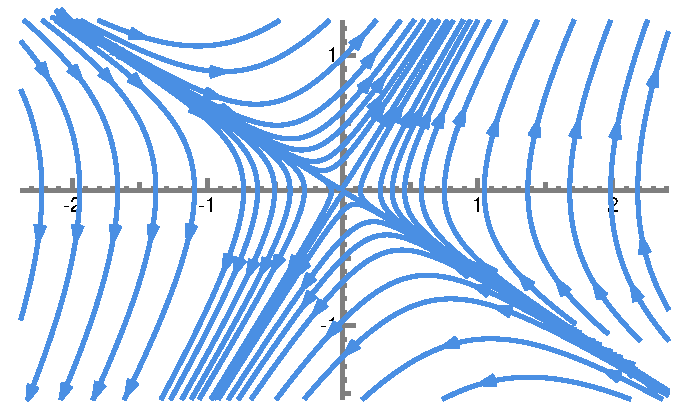
\includegraphics[width=0.75\textwidth]{sistemi_sella.png}
  \caption[1a]{sella (instabile)}
 \end{subfigure}
 \begin{subfigure}{5cm}
  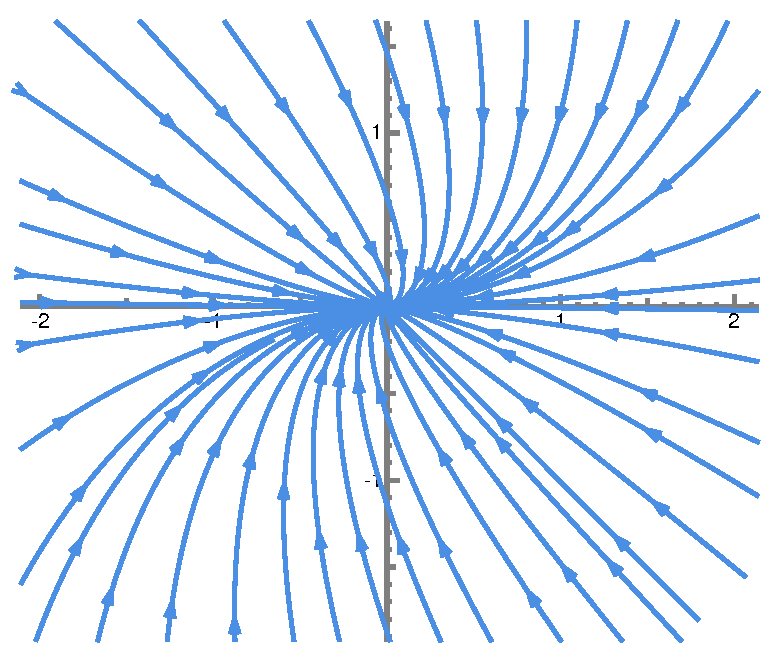
\includegraphics[width=0.75\textwidth]{sistemi_nodo.png}
  \caption{nodo stabile}
 \end{subfigure}
 \begin{subfigure}{5cm}
  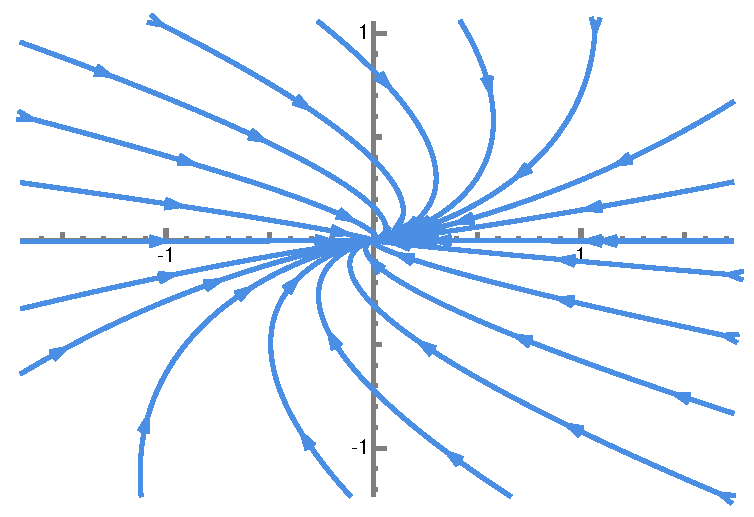
\includegraphics[width=0.75\textwidth]{sistemi_nodo_improprio.png}
  \caption{nodo improprio stabile}
 \end{subfigure}
 \begin{subfigure}{5cm}
  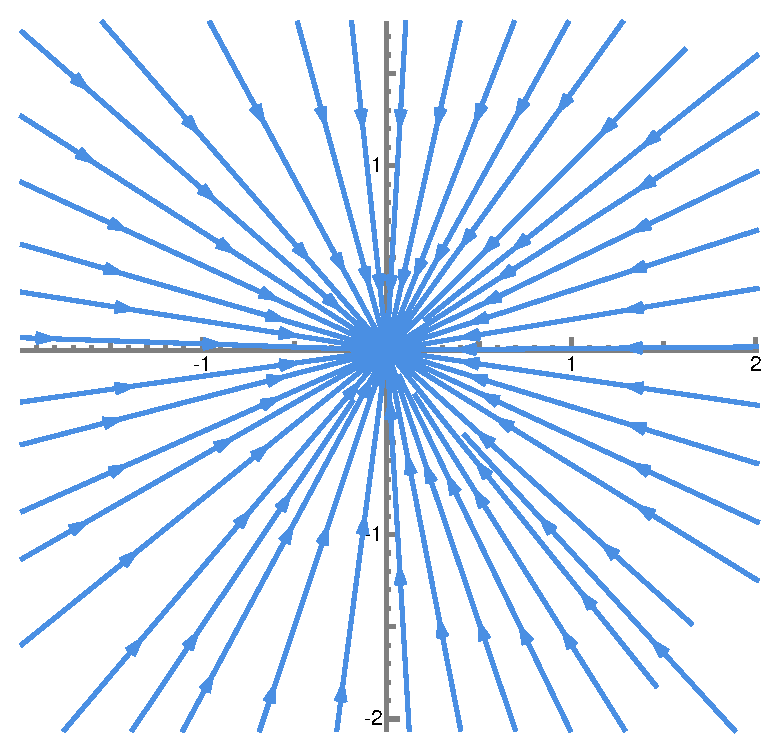
\includegraphics[width=0.75\textwidth]{sistemi_stella.png}
  \caption{stella stabile}
 \end{subfigure}
 \begin{subfigure}{5cm}
  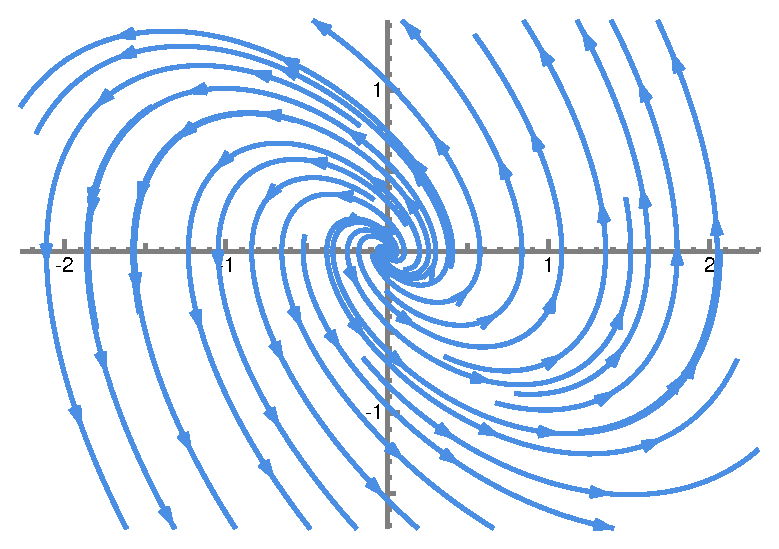
\includegraphics[width=0.75\textwidth]{sistemi_fuoco.png}
  \caption{fuoco stabile}
 \end{subfigure}
 \begin{subfigure}{5cm}
  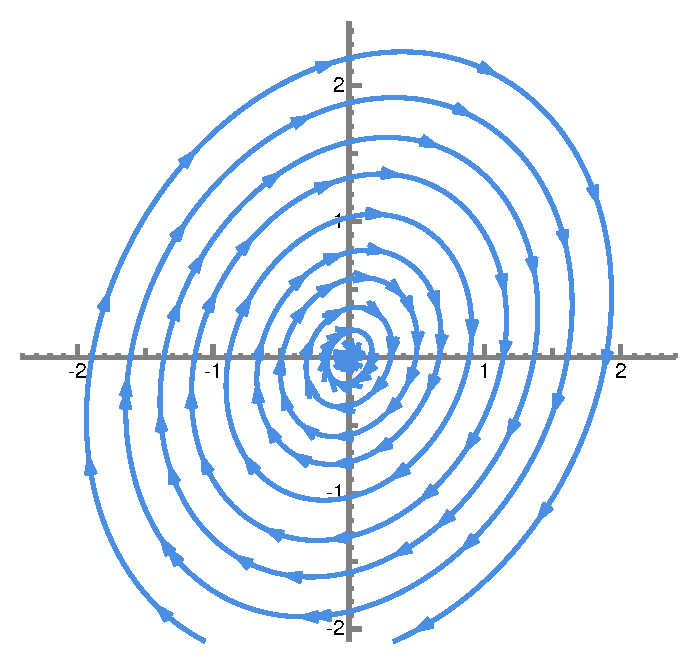
\includegraphics[width=0.75\textwidth]{sistemi_centro.png}
  \caption{centro (stabile)}
 \end{subfigure}
\end{figure}

\emph{Caso 1a.} 
\marginpar{autovalori reali distinti di segno opposto, SELLA}
Se $\mu$ e $\lambda$ hanno segno opposto, allora
$\mu/\lambda<0$ e il grafico della potenze $X^{\mu/\lambda}$ ha
l'andamento di una iperbole (ma una vera iperbole si ottiene solamente
quando $\mu=-\lambda$). 
Le soluzioni in questo caso sono dunque
instabili.
Si dice in questo caso che siamo di fronte ad un punto di \emph{sella}.

\emph{Caso 1b.}
\marginpar{autovalori reali distinti negativi, NODO STABILE}
Se $\mu$ e $\lambda$ sono entrambi negativi, allora il
grafico della potenza $X^{\mu/\lambda}$ ha l'andamento di una parabola
(ma una vera parabola si ottiene solamente quando $\mu=2\lambda$
oppure $\lambda=2 \mu$). Inoltre le curve sono orientate verso
l'origine (infatti le funzioni $X(t)=k_1 e^{\lambda t}$ e $Y(t)=k_2
e^{\mu t}$ tendono entrambe a zero per $t\to +\infty$). Si ha in
questo caso quello che viene chiamato un \emph{nodo asintoticamente
  stabile}.

\emph{Caso 1c.} 
\marginpar{autovalori reali distinti positivi, NODO INSTABILE}
Se $\mu$ e $\lambda$ sono entrambi positivi, allora il
supporto delle curve soluzioni del sistema è lo stesso del caso
precedente. Ma l'orientazione è opposta, per $t\to \infty$ le
traiettorie si allontanano dall'origine e vanno all'infinito. Si parla
in questo caso di \emph{nodo instabile}.

\emph{Caso 2.} 
\marginpar{matrice diagonale, STELLA}
Se la matrice $A$ è della forma
$\diag(\lambda,\lambda)=\lambda I$. Osserviamo che questo è equivalente a dire
 che $A$ ha un unico autovalore $\lambda$ con molteplicità algebrica 2 e
molteplicità geometrica 2 in quanto in tal caso l'autospazio
dell'autovettore $\lambda$ è l'intero spazio e in qualunque base la
matrice risulta essere diagonale.
Il sistema di equazioni differenziali è allora banale:
\[
\begin{cases}
 x' = \lambda x\\
 y' = \lambda y.
\end{cases}
\]
Le soluzioni sono tutte della forma: $x(t)=c_1 e^{\lambda t}$,
$y(t)=c_2 e^{\lambda t}$ le cui traiettorie hanno equazione
$y=\frac{c_2}{c_1}x$ cioè sono delle rette passanti per l'origine.
Se $\lambda<0$ le curve tendono asintoticamente all'origine $(0,0)$ e
si parla in questo caso di \emph{stella asintoticamente stabile}.
Se invece $\lambda>0$ si parla di \emph{stella instabile}. Se $\lambda
= 0$ tutte le soluzioni sono curve costanti, diremo quindi che le
soluzioni sono \emph{degeneri}.

\emph{Caso 3.} 
\marginpar{autovalori coincidenti ma non diagonalizzabile, NODO IMPROPRIO}
Supponiamo che la matrice $A$ abbia un unico autovalore reale
$\lambda$ con molteplicità algebrica 2 ma supponiamo che la matrice
$A$ non sia diagonale. Sia $v$ un autovettore di $A$,
prendo un qualunque vettore $z$ indipendente da $v$ e considero
la base $v,z$. In questa base si ha $Av = \lambda v$, $Az = \alpha v +
\beta z$. Osserviamo che $\beta = \lambda$ in quanto il determinante
della matrice $A$ è $\lambda^2$ ed è invariante per cambio di
base, ma nella base $v,z$ la matrice che rappresenta $A$ è triangolare
ed ha $\lambda,\beta$ sulla diagonale. 

Dunque $Az = \alpha v + \lambda z$. Ora sappiamo
che $\alpha\neq 0$ altrimenti $z$ sarebbe un secondo autovettore,
la molteplicità geometrica dell'autovalore $\lambda$ sarebbe $2$ e $A$
sarebbe diagonale. Dunque
prendiamo $w=z / \alpha$ e otteniamo $Av=\lambda v$, $Aw = v +
\lambda w$. Il vettore $w$ così trovato si chiama \emph{autovettore
  generalizzato} o \emph{pseudo-autovettore}. Ponendo $P=(v,w)$ (la
matrice del cambio di base, le cui colonne sono $v$ e $w$) si ha dunque:
\[
A = P B P^{-1}, \qquad B=\begin{pmatrix}\lambda & 1 \\ 0 & \lambda \end{pmatrix}
\]
e quindi le soluzioni sono:
\[
u(t) = e^{tA}c = P e^{tB}P^{-1}c = P e^{tB}k.
\]
con $k=P^{-1}c$.

La matrice $B$ viene chiamata \emph{forma canonica di Jordan} della matrice $A$.

Osserviamo ora che si può scrivere 
\[
B = \lambda I + N \qquad\text{con}\qquad N=\begin{pmatrix}0&1\\0 & 0\end{pmatrix}.
\]
Da verifica diretta si trova $N^2=0$ e dunque $e^{tN} = I + tN$ (in base
all'ultima delle proprietà dell'esponenziale). Dunque
\begin{align*}
u(t) &= P e^{t\lambda I + tN}k = P e^{t\lambda I} (I + t N)k =
P e^{\lambda t} \begin{pmatrix} 1 & t \\ 0 & 1\end{pmatrix}\begin{pmatrix}k_1\\k_2\end{pmatrix}\\
& = P e^{\lambda t}\begin{pmatrix}k_1 + k_2 t \\ k_2\end{pmatrix}
\end{align*}
da cui, ponendo $u=(x,y) = P(X,Y)$, si trovano le soluzioni nella base
$v,w$:
\[
\begin{cases}
X(t) = (k_1 + k_2 t) e^{\lambda t}\\
Y(t) = k_2 e^{\lambda t}.
\end{cases}
\]
Se $\lambda<0$ le curve tendono all'origine quando $t\to +\infty$ e
abbiamo quindi un comportamento asintoticamente stabile. Se invece
$\lambda>0$ le curve tendono all'infinito e si ha dunque un
comportamento instabile. 
Eliminando la $t$ ($t=\frac 1 \lambda \log\frac Y {k_2}$) e ponendo $a
= \frac{k_1}{k_2} - \frac{\log|k_2|}{\lambda}$ si ottiene 
\[
X(t) = \left(a+\frac{\log|Y(t)|}{\lambda}\right)Y(t).
\]
Si vede che per $Y\to 0$ anche $X\to 0$ ma con pendenza $dx/dy$
infinita. Dunque le curve arrivano all'origine risultando tangenti
all'asse delle $X$. D'altra parte per $k_2=0$ si trovano delle
soluzioni con $Y=0$, dunque anche l'asse delle $x$ contiene soluzioni
dell'equazione.

Se $\lambda=0$ si ha una situazione degenere.

\emph{Caso 4.}
\marginpar{autovalori complessi coniugati}
Se la matrice $A$ è una matrice reale, (cioè coincide con la propria
coniugata: $\overline A=A$) con un autovalore complesso $\lambda =
\alpha + i\beta$, $\beta\neq 0$, con relativo autovettore complesso
$v+iw$, allora si ha 
\[
  A(v+iw) = \lambda(v+iw)
\]
e quindi
\[
  A(v-iw) = \overline{A(v+iw)} = \overline{\lambda(v+iw)} = \bar \lambda (v-iw)
\]
che significa che $\overline \lambda = \alpha-i\beta$ è anch'esso un autovalore e $v-iw$ è l'autovettore associato. Dunque la matrice $A$ è diagonalizzabile nel campo complesso:
\[
  A = P D P^{-1},\qquad P=(v+iw, v-iw),\qquad D = \diag(\alpha+i\beta, \alpha-i\beta)
\]
($P$ è la matrice che ha come colonne i vettori complessi $v+iw$ e
$v-iw$).

Essendo $v+iw$ e $v-iw$ vettori complessi indipendenti, si può
facilmente mostrare che anche i vettori reali $v,w$ risultano essere
indipendenti. Osserviamo allora che
\[
 P = (v+iw, v-iw) = (v,w)\begin{pmatrix}1 & 1\\ i & -i\end{pmatrix}
\]
e che
\[
  P^{-1} = \begin{pmatrix}1 & 1\\ i & -1\end{pmatrix}^{-1}(v,w)^{-1}
         = \frac 1 2 \begin{pmatrix}1 & -i\\ 1 & i\end{pmatrix}(v,w)^{-1}
\]
e quindi nella base $v,w$ la matrice $A$ diventa:
\begin{align*}
\frac 1 2
\begin{pmatrix}1 & 1\\ i & -i\end{pmatrix}
\begin{pmatrix}\lambda & 0 \\ 0 & \bar \lambda\end{pmatrix}
\begin{pmatrix}1 & -i\\ 1 & i\end{pmatrix}
&=
\frac 1 2
\begin{pmatrix}\alpha+i\beta & \alpha-i\beta \\i\alpha-\beta  &
  -i\alpha-\beta\end{pmatrix}
\begin{pmatrix}1 & -i\\ 1 & i\end{pmatrix}\\
&=
\begin{pmatrix}\alpha & \beta \\-\beta  & \alpha\end{pmatrix}.
\end{align*}

Osserviamo qui che la matrice $A$ è diagonalizzabile in campo
complesso, ma non in campo reale. Una rappresentazione \emph{canonica}
di $A$ nel campo reale è quella data qui sopra, e viene chiamata
\emph{forma canonica reale di Jordan}. I vettori $v,w$ che sono parte reale
e parte immaginaria degli autovettori complessi di $A$, possono anche
essere identificati dalle seguenti proprietà:
\[
  Av = \alpha v - \beta w,\qquad Aw = \beta v + \alpha w.
\]

Le soluzioni del sistema sono dunque, al variare di $c\in \RR^2$:
\begin{align*}
u(t) & = e^{tA} c = P e^{tD}P^{-1} c
       = P e^{tD} \frac 1 2 \begin{pmatrix}1 & -i\\ 1 & i\end{pmatrix} k
\end{align*}
dove si è posto $k=(v,w)^{-1} c$. Dunque
\begin{align*}
  u(t) &= \frac 1 2 P \begin{pmatrix}e^{\lambda t} & 0 \\ 0 & e^{\bar \lambda t}\end{pmatrix}
          \begin{pmatrix}k_1 - ik_2\\ k_1 + i k_2\end{pmatrix}\\
 &= \frac 1 2 P \begin{pmatrix}e^{\alpha t + i \beta t}(k_1-ik_2) \\ e^{\alpha t - i \beta t}(k_1 + i k_2)\end{pmatrix} \\
 &= \frac 1 2 P e^{\alpha t}\begin{pmatrix} e^{i\beta t}(k_1-ik_2) \\
  e^{-i\beta t}(k_1 + ik_2)\end{pmatrix}.
\end{align*}
Scrivendo il numero complesso $k_1 + i k_2$ in coordinate polari si potranno trovare $\rho$ e $\phi$ tali
che $k_1 + i k_2 = \rho e^{-i\phi}$. Si avrà allora
\begin{align*}
u(t) 
&= 
\frac 1 2 \rho e^{\alpha t}P\begin{pmatrix}
e^{i\beta t} e^{i\phi} \\
e^{-i\beta t} e^{-i\phi}
\end{pmatrix}\\
&= 
\frac 1 2 \rho e^{\alpha t} (v,w)
\begin{pmatrix}1 & 1 \\ i & -i\end{pmatrix} 
\begin{pmatrix}
e^{i(\beta t+\phi)} \\
e^{-i(\beta t+\phi)}
\end{pmatrix}\\
& =
\frac 1 2 (v,w) \rho e^{\alpha t} 
\begin{pmatrix}
e^{i(\beta t+\phi)} + e^{-i(\beta t+\phi)}\\
ie^{i(\beta t+\phi)} - ie^{-i(\beta t+\phi)}
\end{pmatrix}\\
&=
(v,w)
\begin{pmatrix}
\rho e^{\alpha t}
\cos(\beta t+\phi))\\
-\rho e^{\alpha t}
\sin(\beta t+\phi))
\end{pmatrix}
\end{align*}
da cui, se $X,Y$ sono le coordinate di $u(t)$ nella base $v,-w$, si ha
\begin{align*}
X(t) &= \rho e^{\alpha t} \cos(\beta t+\phi))\\
Y(t) &= \rho e^{\alpha t} \sin(\beta t+\phi)),
\end{align*}
dove, ricordiamo, $\alpha$ e $\beta$ sono parte reale e parte
immaginaria del primo autovalore complesso, mentre $\rho\ge 0$ e $\phi\in[0,2\pi)$
(ampiezza e fase) sono parametri arbitrari ognuno dei quali ci
fornisce una diversa soluzione.

Se $\alpha=0$ 
\marginpar{CENTRO (stabile)}
(cioè i due autovalori di $A$ sono immaginari puri)
allora le soluzioni descrivono nel piano $X,Y$ dei cerchi concentrici
centrati nell'origine. Nel piano $x,y$ saranno dunque delle ellissi
con gli assi paralleli ai vettori $v$ e $w$. Questa configurazione si
chiama \emph{centro} ed è una configurazione \emph{stabile} (ma non
asintoticamente)
nel senso che le traiettorie rimangono limitate, pur non convergendo
all'origine.

Se $\alpha<0$
\marginpar{FUOCO asintoticamente stabile}
le traiettorie descrivono delle spirali logaritmiche che convergono
verso l'origine. Il verso di rotazione è da $w$ verso $v$ se $\beta$ è
positivo, da $v$ verso $w$ se $\beta$ è negativo.
Si dice allora che siamo in presenza di un
\emph{fuoco asintoticamente stabile}.

Se $\alpha>0$
\marginpar{FUOCO instabile}
le traiettorie descrivono delle spirali che si allontanano
dall'origine divergendo all'infinito. Il senso di rotazione è
determinato da $\beta$ come nel caso precedente.
Questa configurazione è chiamata \emph{fuoco asintoticamente instabile}.

\section*{Aggiornamenti}
\begin{itemize}
\item[13.12.2014] aggiunte figure e revisione generale.
\item[12.9.2015] piccoli aggiustamenti.
\end{itemize}
\end{document}

\input{chapters/edo/modelli}
\section{studio qualitativo delle soluzioni}
\label{sec:studio_qualitativo_edo}

Non sempre è possibile determinare esplicitamente le soluzioni
di una equazione differenziale.
Ci proponiamo quindi di trovare dei metodi per
determinare alcune proprietà salienti delle soluzioni, senza
doverle determinare esplicitamente.
Considereremo unicamente equazioni del primo ordine in forma normale:
\begin{equation}\label{eqdiff}
	u'(x)= f(x,u(x))
\end{equation}
con $f\colon \Omega \subset \RR^2\to \RR$.

Ricordiamo che se $f$ soddisfa la condizione di Cauchy-Lipschitz
(definizione~\ref{def:cauchy_lipschitz}), in particolare
se $f$ è di classe $C^1$ allora i grafici delle soluzioni
massimali dell'equazione differenziale~\eqref{eqdiff}
\emph{fibrano} la regione $\Omega$ nel senso che per ogni punto di
$\Omega$ passa una unica soluzione massimale (teorema~\ref{th:cauchy_lipschitz}
di Cauchy-Lipschitz e proposizione~\ref{prop:separazione_soluzioni}).
Inoltre la proposizione~\ref{prop:edo_massimale} ci dice
che le soluzioni massimali escono da qualunque compatto contenuto in
$\Omega$ ovvero raggiungono sempre la frontiera di $\Omega$.

\begin{example}\label{ex:edo_4630b}
Sia $u$ la soluzione massimale del problema di Cauchy
\[
	\begin{cases}
		u' = \cos(u^2)\cdot \sin x, \\
		u(0) = 0.
	\end{cases}
\]
Mostrare che $u$
è definita su tutto $\RR$ (dunque la soluzione è globale).
Mostrare che $u$ è pari.
Mostrare che $u$ è periodica.
Mostrare che $u(x)\ge 0$ per ogni $x\in \RR$.
\end{example}
\newsavebox{\qredoquattro}\sbox{\qredoquattro}{%
\myqrshortdoclink{edo_4630b}{Studio qualitativo esempio \getrefnumber{ex:edo_4630b}}}
\begin{figure}
  \centering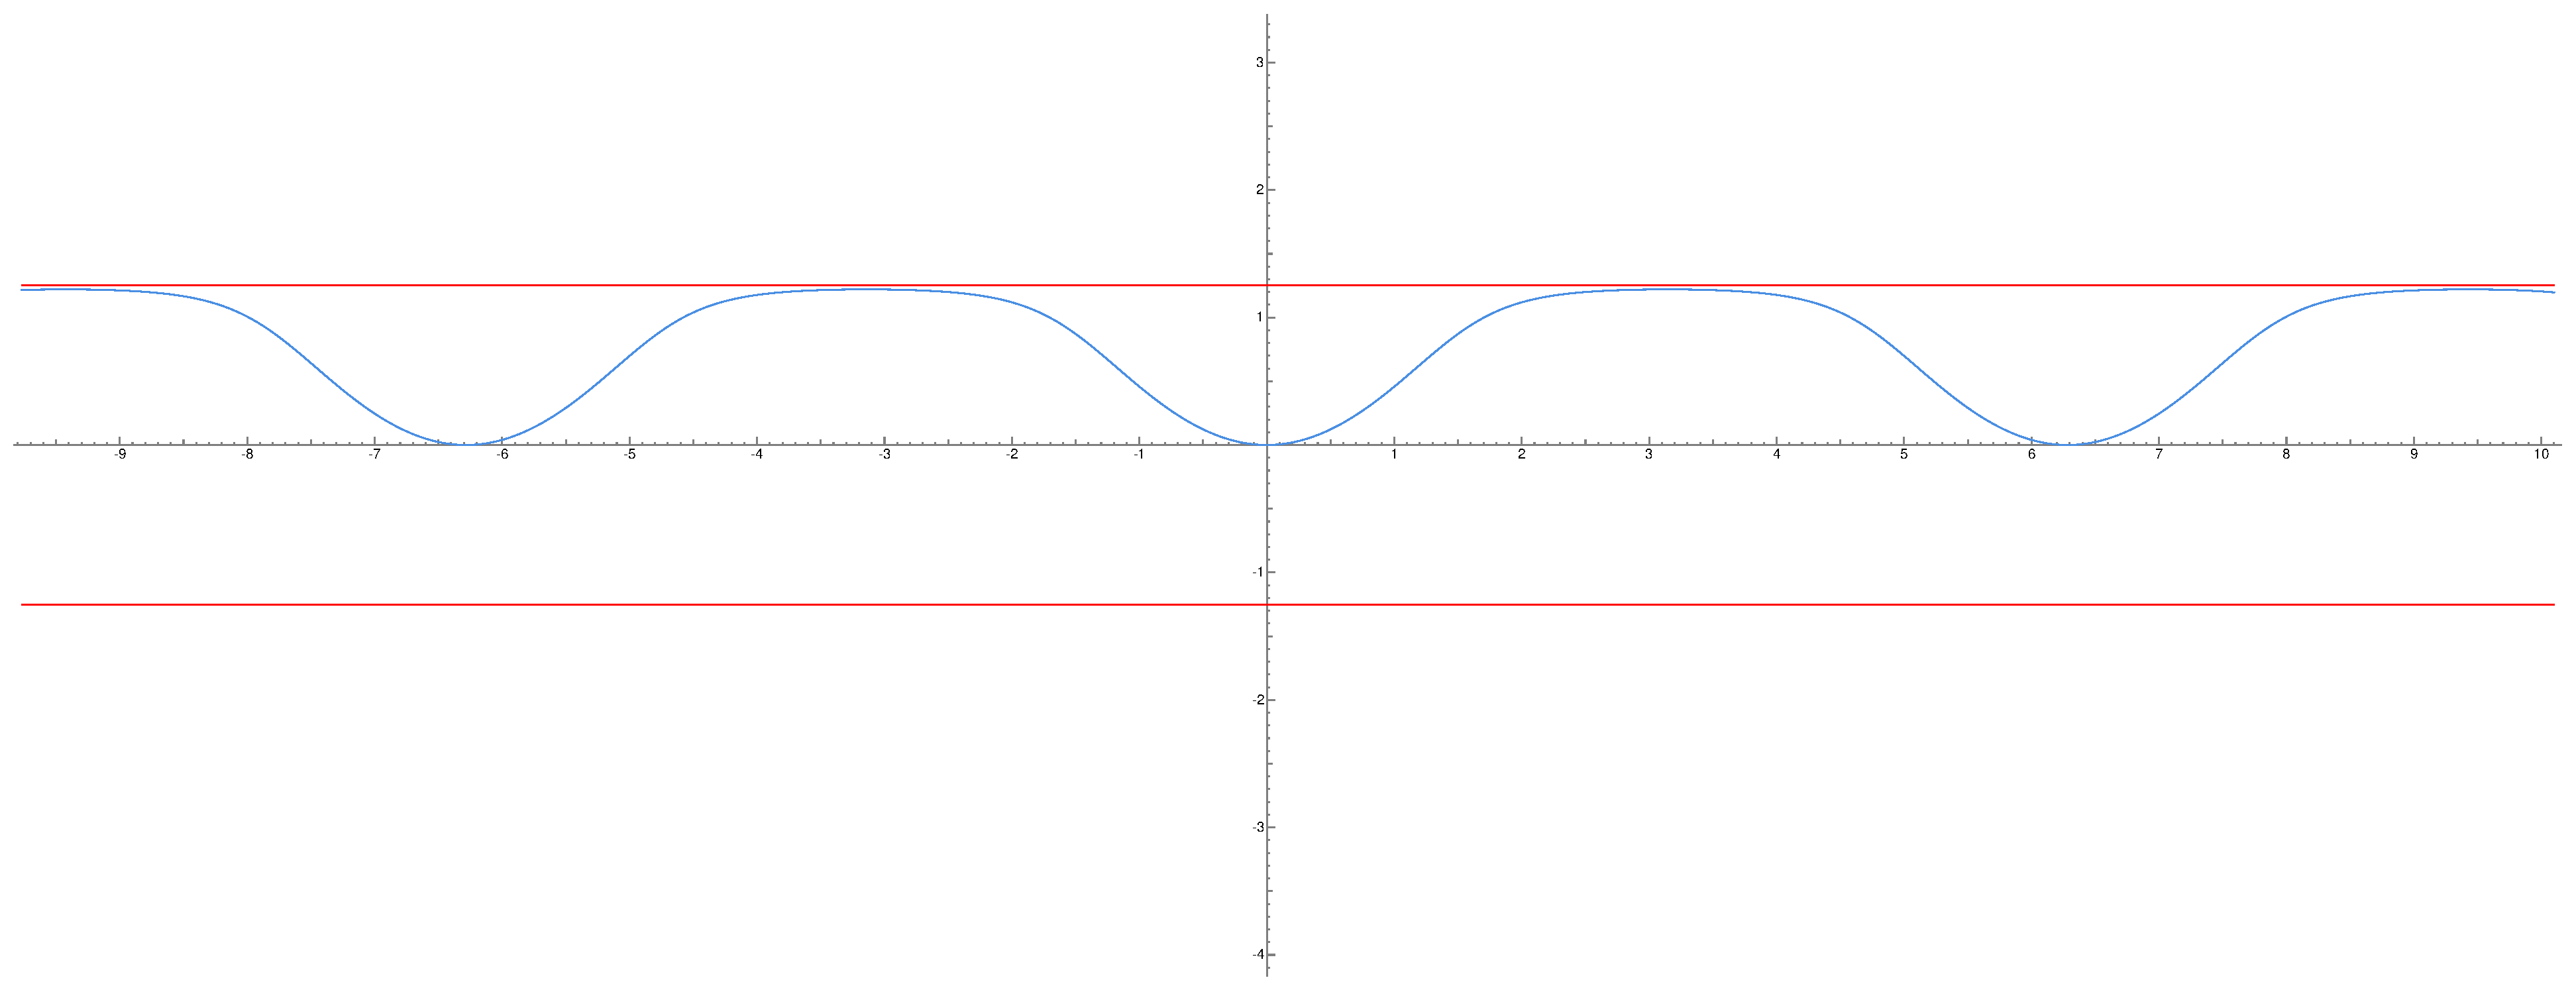
\includegraphics[width=\textwidth]{edo_4630b}
  \caption{Studio qualitativo dell'esempio~\ref{ex:edo_4630b}.
  \ifwidemargin\\\\\fi%
  \usebox{\qredoquattro}}
  \label{fig:edo_4630b}
\end{figure}
%
\begin{proof}[Svolgimento.]
In questo caso si ha $f(x,y)=\cos y^2\cdot \sin x$, che \`e una funzione
di classe $C^1$ su tutto $\Omega=\RR^2$.
Vale dunque il teorema di esistenza ed
unicità delle soluzioni.
Notiamo inoltre (per verifica diretta)
che posto $H=\sqrt{\frac \pi 2}$, le funzionie 
costanti $u_0(x)=-H$ e $u_1(x)=H$ sono
soluzioni dell'equazione differenziale (\ref{eqdiff})
in quanto $f\enclose{x,\pm H}=0$ per ogni $x\in \RR$
(soluzioni \emph{stazionarie}).
Per la proposizione~\ref{prop:separazione_soluzioni},
il grafico della soluzione $u(x)$
non può toccare i grafici delle due funzioni $u_0$ e $u_1$ e visto
che $u(0)=0$ e che $u$ è una funzione continua significa
che per ogni $x$ si ha $-H < u(x) < H$.
Consideriamo ora il compatto
$K_M=[-M,M] \times [-H,H]$.
Sappiamo che la soluzione
massimale $u(x)$ del problema di Cauchy preso in considerazione deve
uscire da ogni compatto $K_M$
(proposizione~\ref{prop:edo_massimale}).
Visto però che $u(x)\in (-H,H)$ significa che necessariamente
il grafico della soluzione massimale $u(x)$
raggiunge i due segmenti verticali
$x=-M$ e $x=M$ e dunque l'intervallo massimale di esistenza
contiene l'intervallo $[-M,M]$.
Siccome questo è vero per ogni $M$, l'intervallo massimale
di esistenza della soluzione è $I=\RR$ e dunque la soluzione
è globale.

Dimostriamo che $u$ è pari. Sia $v(x)=u(-x)$. 
Si ha 
\[ 
    v'(x) = -u'(-x) 
    = -\cos(u^2(-x))\cdot \sin(-x) 
    = \cos(v^2(x))\cdot \sin(x)
\]
da cui risulta che $v$ soddisfa la stessa equazione differenziale 
di cui $u$ è soluzione. 
Inoltre $v(0)=u(0)=0$ e quindi $u$ e $v$ sono soluzioni dello 
stesso problema di Cauchy. Per unicità della soluzione 
deve essere $u(x)=v(x)$ per ogni $x$ e quindi $u(-x)=u(x)$, come 
volevamo dimostrare.
  
Dimostriamo ora che $u$ è $2\pi$-periodica.
Sia $w(x)=u(x+2\pi)$. Si ha allora 
\[
  w'(x) = u'(x+2\pi) = \cos(u^2(x+2\pi))\cdot \sin(x+2\pi) 
  = \cos(w^2(x))\cdot \sin(x) 
\]
dunque, di nuovo, $w$ soddisfa la stessa equazione differenziale
di cui $w$ è soluzione. Si ha inoltre 
\[
  u(-2\pi) - w(-2\pi) = u(2\pi) - u(0) = w(0) - u(0).
\]
Questo significa che $u-v$ assume segno opposto nei punti 
$a=-2\pi$ e $b=0$ e quindi, per il teorema~\ref{th:valori_intermedi}
dei valori intermedi ci deve essere un punto in cui le due 
$u-v$ si annulla. In tale punto ho due soluzioni dello stesso 
problema di Cauchy e dunque, per l'unicità della soluzione, 
dobbiamo concludere che $u(x)=v(x)$ per ogni $x$.
Questo significa che $u$ è $2\pi$-periodica.

Visto che $\abs{u(x)}<H$ con $H^2=\pi 2$ si ha che $\cos(u^2(x))>0$ 
e quindi $u'(x)$ ha lo stesso segno di $\sin x$: sull'intervallo 
$[0,\pi]$ la funzione $u(x)$ è crescente e su $[\pi,2\pi]$ è decrescente.
Visto che $u$ è $2\pi$-periodica si ha che $u(2\pi)=u(0)=0$ e quindi 
$0$ è il valore minimo assunto da $u$.

Si veda la figura~\ref{fig:edo_4630b}.
\end{proof}

\subsection{monotonia e punti critici delle soluzioni}

Dopo aver determinato le zone di $\Omega$ su cui vale il teorema di
esistenza e unicit\`a, \`e utile studiare il segno di $f$. Infatti
le soluzioni $u(x)$ dell'equazione differenziale (\ref{eqdiff})
saranno strettamente crescenti dove $f>0$, strettamente decrescenti
dove $f<0$ e avranno un punto critico dove $f=0$.

Un primo caso notevole è il caso in cui $f$ si annulla su una
retta orizzontale $y=c$.
In questo caso la funzione costante $u(x)=c$ è una
soluzione dell'equazione differenziale (\ref{eqdiff}).
Inoltre
(nell'ipotesi $f\in C^1$) tale costante non può essere
attraversata dalle altre soluzioni dell'equazione differenziale.

\`E importante capire se le soluzioni dell'equazione differenziale
attraversano o no la curva $\{f=0\}$. Infatti questo ci permette di
determinare il segno della derivata $u'(x)$ e quindi di ottenere
importanti informazioni sull'andamento della soluzione $u(x)$
(monotonia, massimi e minimi relativi...).

Più in generale è interessante capire quando una soluzione di una
equazione differenziale può attraversare una determinata curva.

\begin{theorem}\label{nonpassa}
Sia $u(x)$ una soluzione dell'equazione differenziale $(\ref{eqdiff})$
definita su un intervallo $I$ e sia $v(x)$ una funzione qualunque
definita su $I$, di classe $C^1$ e tale che il suo grafico sia
interamente contenuto nel dominio $\Omega$ di definizione di $f$.
Supponiamo che in un punto fissato $x_0$ interno ad $I$ si abbia
$u(x_0)<v(x_0)$ e supponiamo inoltre che per ogni $x>x_0$ si abbia
$v'(x)>f(x,v(x))$. Allora per ogni $x>x_0$ si ha $u(x)<v(x)$.

Analogamente se $u(x_0)>v(x_0)$ e se per ogni $x$ si ha
$v'(x)<f(x,v(x))$ risulterà $u(x)>v(x)$ per ogni $x>x_0$.

Risultati analoghi si hanno per $x<x_0$.
\end{theorem}

\begin{proof}
Supponiamo per assurdo che l'insieme $J=\{x\in I: x\ge x_0\
\mathrm{e}\ u(x)=v(x)\}$ non sia vuoto.
Tale insieme è chiuso ed
inferiormente limitato, quindi se non è vuoto, ammette minimo.
Sia $\bar x$ il minimo di $J$.
Sicuramente $\bar x>x_0$ in quanto $u(\bar
x)=v(\bar x)$.
Inoltre per ogni $x\in \left[x_0,\bar x\right[$ si ha
$u(x)-v(x)<0$ e quindi $u'(\bar x) \ge v'(\bar x)$ (in quanto
il rapporto incrementale sinistro di $u-v$ è sempre positivo).

Questo è assurdo in quanto per ipotesi si ha invece $u'(\bar x) =
f(\bar x, u(\bar x)) = f(\bar x ,v(\bar x)) < v'(\bar x)$.
\end{proof}

Se ad esempio $v(x)$ è una funzione
il cui grafico è contenuto in $\{f=0\}$
(cioé $f(x,v(x))=0$) allora una soluzione $u(x)$ dell'equazione
differenziale può attraversare la curva $v(x)$ dall'alto verso il
basso nei punti in cui $v'(x)>0$ e dal basso verso l'alto nei punti
in cui $v'(x)<0$.

\newsavebox{\qrexoqt}\sbox{\qrexoqt}{%
\myqrshortdoclink{qrexoqt}{il grafico della soluzione dell'esempio \getrefnumber{ex843}}}
\begin{figure}
\centering
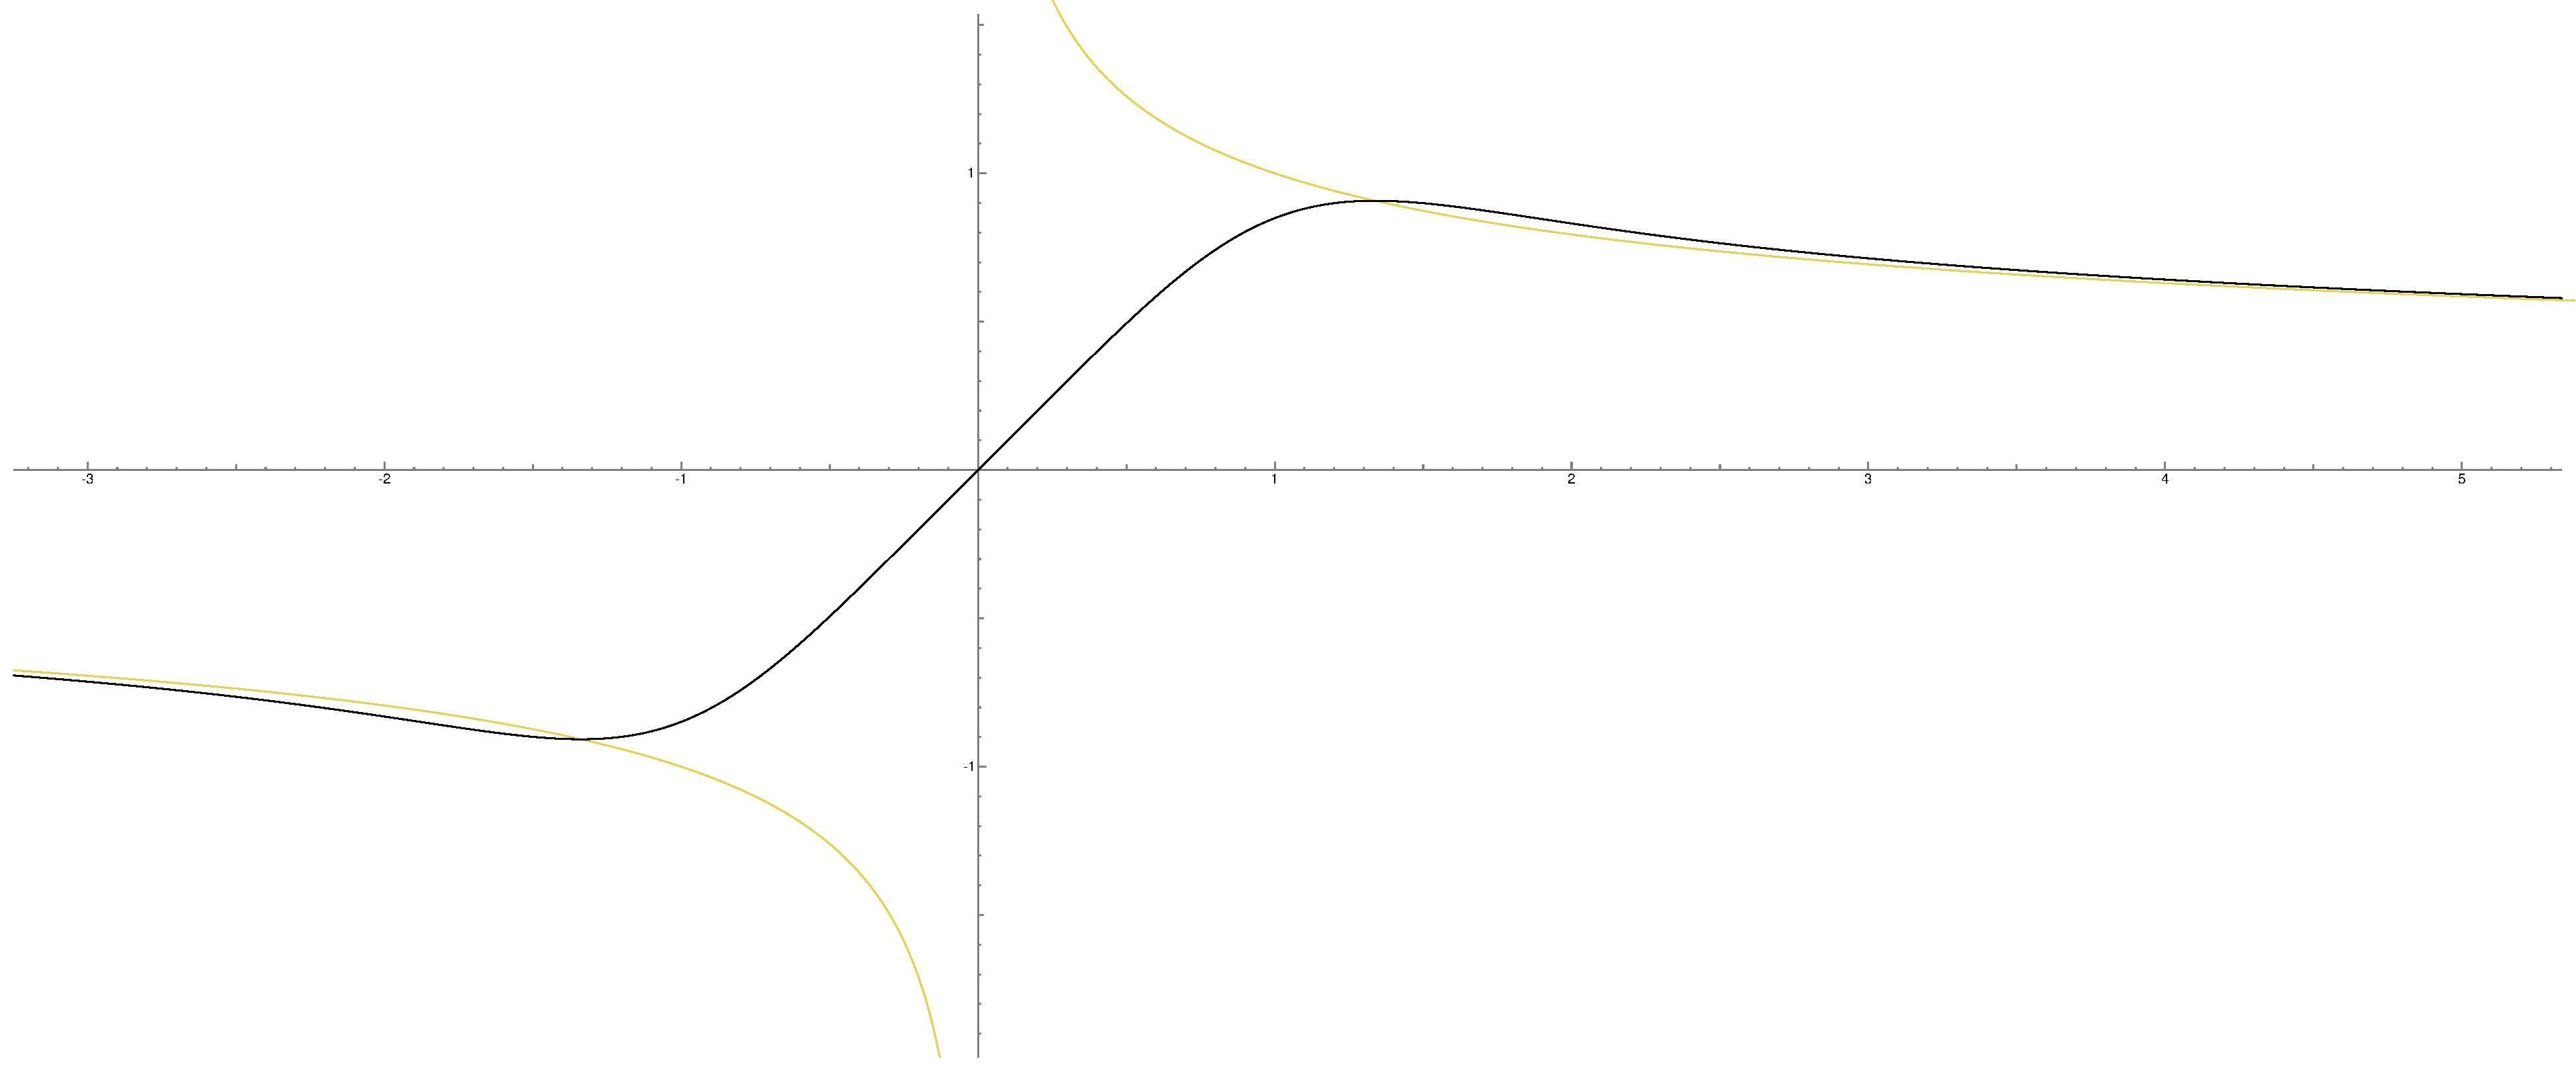
\includegraphics[width=0.8\textwidth]{ex843.pdf}
\caption{Il grafico della soluzione del problema di Cauchy nell'esempio~\ref{ex843}
\ifwidemargin\\\\\fi%
\usebox{\qrexoqt}}
\label{fig:ex843}
\end{figure}
%
\begin{example}\label{ex843}
Si consideri il seguente problema di Cauchy
\[
\begin{cases}
  u'=1-x u^3\\
  u(0)=0
\end{cases}
\]
ammette una soluzione $u(x)$ definita su tutto $\RR$.
\end{example}
%
\begin{proof}[Svolgimento.]
Posto $f(x,y)=1 - xy^3$ abbiamo che $f$ si annulla sul grafico della
funzione $u_0(x)=1/\sqrt[3] x$. Per $x>0$ la soluzione è crescente
quando si trova al di sotto della funzione $u_0$ ed è decrescente
quando si trova al di sopra. Inoltre essendo $u_0'<0$ le soluzioni possono
attraversare la funzione $u_0(x)$ solo passando da sotto a
sopra.

Sia $u(x)$ la soluzione del problema di Cauchy in questione, definita su
un intervallo massimale $I$. Il dato
iniziale è $(0,0)\in \{f>0\}$. Dunque la soluzione risulta essere
strettamente crescente in un intorno di $0$.

Vogliamo dimostrare innanzitutto che necessariamente la soluzione
incontra entrambi i rami del grafico di $u_0(x)$. Sia infatti
$\eps>0$ sufficientemente piccolo da appartenere all'intervallo
$I$ di
esistenza della soluzione e sia $\delta=u(\eps)$.
Consideriamo il compatto $K=\{(x,y):
\eps/2 \le x \le 1/\delta^2,\ 0\le y\le 1/\sqrt[3]{x}\}$. Il punto
$(\eps,u(\eps))$ è interno al compatto $K$ ma la soluzione deve
uscire dal compatto
per un qualche $x>\eps$.
La soluzione però non può toccare la
retta $y=0$ in quanto all'interno del compatto rimane sempre positiva
e crescente.
Non può neanche toccare il segmento verticale
$x=1/\delta^2$, $y\in[0,\delta]$ in quanto $u(\eps)=\delta$ e per
$x>0$ la soluzione è strettamente crescente.
Dunque necessariamente
la soluzione deve incontrare il grafico della funzione
$u_0(x)=1/\sqrt[3]{x}$ in un punto $\bar x>0$.

Nel punto $x=\bar x$ la soluzione $u(x)$ attraversa la curva
$u_0(x)$. Infatti in tale punto $u'(\bar x)=0$ mentre $u_0'(\bar
x)<0$.
Dunque in un intorno destro di $\bar x$ la soluzione si trova
al di sopra della curva $u_0(x)$ e quindi risulta essere decrescente
(in $\bar x$ la soluzione presenta un massimo relativo).

Il Teorema~\ref{nonpassa} garantisce inoltre che la soluzione non
può più riattraversare il grafico della funzione $u_0$ in quanto
$u'_0<0$. Dunque la soluzione è decrescente e limitata.
Dunque (usando come al solito la proposizione~\ref{prop:edo_massimale})
possiamo dedurre che la soluzione massimale è definita per ogni $x>0$.

Un ragionamento analogo si fa per $x<0$ ottenendo l'esistenza globale
della soluzione.
\end{proof}

\begin{example}
Dimostriamo che il problema di Cauchy
\[
\begin{cases}
	u' = -x(u^3 - \sin x) \\
	u(0) = 0
\end{cases}
\]
ammette una soluzione $u(x)$ definita su tutto $\RR$.
\end{example}
%
\begin{proof}
Sia $u(x)$ la soluzione massimale del problema di Cauchy
definita su un intervallo massimale $I$.

Mostriamo innanzitutto che $\vert u(x) \vert < 2$ per ogni $x\in
I$.
Infatti per $x>0$ sulla curva $u_1(x)=2$ si ha $f(x,2) = -x
(8-\sin x) < -x < 0 = u_1'(x)$.
Dunque per il Teorema~\ref{nonpassa} la
soluzione per $x>0$ non può mai attraversare la retta
$y=2$.
Discorso analogo si fa per la retta $y=-2$ e anche per $x<0$
mostrando che il grafico della  soluzione non può mai toccare le
rette $y=2$ e $y=-2$ né per $x>0$ né per $x<0$
e che quindi $u(x)$ risulta limitata (in realtà si
può essere più precisi e mostrare che $\vert u(x)\vert \le 1$).

A questo punto si applica, come al solito, il Teorema~\ref{prop:edo_massimale} ai
compatti $K_M=[-M,M]\times[-2,2]$ mostrando che la soluzione deve
avere esistenza globale.
\end{proof}

\subsection{teoremi di confronto}

\begin{theorem}
Sia $I\subset \RR$ un intervallo su cui sono definite due funzioni derivabili
$f(x)$ e $g(x)$.
Siano $x_1<x_2$ due punti di $I$. Se $f(x_1)<g(x_1)$ e $f(x_2)>g(x_2)$
allora esiste un punto $\bar x \in (x_1,x_2)$ tale che $f(\bar
x)=g(\bar x)$ e $f'(\bar x)\ge g'(\bar x)$.
\end{theorem}

\begin{theorem}
Consideriamo due funzioni $u(x)$ e $v(x)$ soluzioni dei rispettivi
problemi di Cauchy
\[
\begin{cases}
  u'(x)  = f(x,u(x))\\
  u(x_0) = u_0
\end{cases}
\qquad
\begin{cases}
  v'(x) = g(x,v(x))\\
  v(x_0) = v_0
\end{cases}
\]
su un intervallo $I$ che contiene il punto $x_0$.
Sia $\Omega\subset \RR^2$ un sottoinsieme degli insiemi di definizione
di $f$ e $g$ tale che i grafici delle soluzioni $u(x)$ e $v(x)$ siano
contenuti in $\Omega$ al variare di $x\in I$.
Supponiamo che per ogni $(x,y)\in\Omega$ si abbia $f(x,y)<g(x,y)$.
Allora per ogni $x\in I$, $x> x_0$ si ha $u(x)< v(x)$ mentre per ogni
$x\in I$, $x<x_0$ si ha $u(x)>v(x)$.
\end{theorem}

\begin{theorem}
Sia $f\colon (x_0,+\infty)\to \RR$ una funzione di classe
$C^1$ tale
che il limite
\[
  \lim_{x\to +\infty} f'(x) = \ell
\]
esiste, finito o infinito. Se $\ell\neq 0$ allora $f$ non può avere
un asintoto orizzontale per $x\to +\infty$.
\end{theorem}


\appendix

\appendix
\chapter{Listati}

Il seguente codice è scritto in \myemph{python}, un linguaggio di programmazione
molto semplice e pulito che permette, tra l'altro, di utilizzare diverse librerie
utili per il calcolo numerico e scientifico.

\lstset{% general command to set parameter(s)
  basicstyle=\tiny, % print whole listing small
  keywordstyle=\color{black}\bfseries\underbar,
  % underlined bold black keywords
  identifierstyle=, % nothing happens
  commentstyle=\color{white}, % white comments
  stringstyle=\ttfamily, % typewriter type for strings
  showstringspaces=false} % no special string spaces

\section{series.py}

Vedi esempio~\ref{ex:52573}.
\myqrcode{https://github.com/paolini/AnalisiUno/blob/master/code/series.py}{github}{series.py}
\label{code:series}
\lstinputlisting{code/series.py}


\section{bisection.py}

Vedi esempio~\ref{ex:75445}.
\myqrcode{https://github.com/paolini/AnalisiUno/blob/master/code/bisection.py}{github}{bisection.py}
\label{code:bisection}
\lstinputlisting{code/bisection.py}

\newpage

\section{compute\_e.py}

Vedi tabella~\ref{fig:cifre_e}.
\myqrcode{https://github.com/paolini/AnalisiUno/blob/master/code/compute_e.py}{github}{compute_e.py}
\label{code:compute_e}
\lstinputlisting{code/compute_e.py}

\section{Mandelbrot.py}

Vedi figura~\ref{fig:mandelbrot}.
\myqrcode{https://github.com/paolini/AnalisiUno/blob/master/code/Mandelbrot.py}{github}{Mandelbrot.py}
\label{code:Mandelbrot}
\lstinputlisting{code/Mandelbrot.py}

\newpage

\section{compute\_pi.py}

Vedi osservazione~\ref{rem:cifre_pi}.
\myqrcode{https://github.com/paolini/AnalisiUno/blob/master/code/compute_pi.py}{github}{compute_pi.py}
\label{code:compute_pi}
\lstinputlisting{code/compute_pi.py}

\section{Koch.py}

Vedi figura~\ref{fig:koch}.
\myqrcode{https://github.com/paolini/AnalisiUno/blob/master/code/Koch.py}{github}{Koch.py}
\label{code:Koch}
\lstinputlisting{code/Koch.py}

\newpage
\section{Fourier.py}

Vedi figura~\ref{fig:fourier}
\myqrcode{https://github.com/paolini/AnalisiUno/blob/master/code/Fourier.py}{github}{Fourier.py}
\label{code:Fourier}
\lstinputlisting{code/Fourier.py}


\backmatter

\nocite{Giusti}
\nocite{Courant}
\nocite{Marcellini}
\nocite{Rudin}
\nocite{PaganiSalsa}
\nocite{appunti_logica}


\bibliography{biblio}{}
\bibliographystyle{plain}

\printindex

\end{document}
